% Diese Datei ist Teil des Buchs "Schreibe Dein Programm!"
% Das Buch ist lizensiert unter der Creative-Commons-Lizenz
% "Namensnennung - Weitergabe unter gleichen Bedingungen 4.0 International (CC BY-SA 4.0)"
% https://creativecommons.org/licenses/by-sa/4.0/deed.de

\documentclass{tup}

\setstretch{1.2} % 10pt has 12pt baselineskip

% FIXME: Guillemets

\usepackage[utf8]{inputenc}
\usepackage{german}
\usepackage{pifont}
\usepackage{bold-extra}
\usepackage{graphicx}
\usepackage{float}
\usepackage{xcolor}
\usepackage{hhline}
\usepackage{psfrag}
\usepackage{tikz}
\usepackage{bibgerm}
\usepackage{amssymb}
\usepackage{stmaryrd}
\usepackage{prooftree} % für Regeln im Kalkül...
\usepackage{mdframed}
\usepackage{theorem}
\theoremstyle{plain}
\usepackage{thmtools,thm-restate}
\usepackage{amsmath}
\usepackage{eurosym}
\usepackage{alltt}
\usepackage{listings}
\lstset{
  language=SdP
}
\usepackage{verbatim}
\usepackage{fancybox}
\usepackage{tabularx}
\usepackage{url}
\usepackage[matrix,frame,arrow]{xy}
\usepackage{makeidx}
\usepackage{longtable}
\usepackage{hyperref}
\usepackage{textcomp}
\usepackage{theorem}
%\usepackage{showframe}

\makeindex
% Diese Datei bitte selbst anlegen mit etwaigen
% \includeonly-Statements.
\input{includeonly}

% from lmodern.sty
% this gives us bold typewriter
\renewcommand{\ttdefault}{lmtt}

\theorembodyfont{\normalfont}
\theoremheaderfont{\normalfont\sffamily\scshape}

\theoremstyle{plain}

\theorembodyfont{\normalfont}
\theoremheaderfont{\normalfont\sffamily\scshape}

\newtheorem{satz}{Satz}[chapter]
\renewcommand{\thesatz}{\thechapter.\arabic{satz}}

\newtheorem{lemma}[satz]{Lemma}
\renewcommand{\thelemma}{\thechapter.\arabic{lemma}}

\newtheorem{korollar}[satz]{Korollar}
\renewcommand{\thekorollar}{\thechapter.\arabic{korollar}}

\theorembodyfont{\normalfont}
\newtheorem{definition}[satz]{Definition}
\renewcommand{\thedefinition}{\thechapter.\arabic{definition}}

\newtheorem{aufgabe}{Aufgabe}[chapter]
\renewcommand{\theaufgabe}{\thechapter.\arabic{aufgabe}}

\newtheorem{bemerkung}[satz]{Bemerkung}
\renewcommand{\thebemerkung}{\thechapter.\arabic{bemerkung}}

\theorembodyfont{\small\normalfont\fontsize{9pt}{11pt}}
\theoremheaderfont{\small\sffamily\scshape}
\newtheorem{beispiel}[satz]{Beispiel}
\renewcommand{\thebeispiel}{\thechapter.\arabic{beispiel}}

\theorembodyfont{\normalfont}
\theoremheaderfont{\normalfont\sffamily\scshape}

\newtheorem{mantra}{Mantra}%[chapter]

\newtheorem{xkonstruktionsanleitung}{Konstruktionsanleitung}%[chapter]
\newenvironment{konstruktionsanleitung}[1]
  {\begin{mdframed}[backgroundcolor=lightgray]\begin{xkonstruktionsanleitung}[#1]}%
  {\end{xkonstruktionsanleitung}\end{mdframed}}

\newcommand{\deq}{\stackrel{\rm def}{=}}
\newcommand{\diff}{\stackrel{\rm def}{\Longleftrightarrow}}
\newcommand{\enn}{\mathbb{N}}
\newcommand{\err}{\mathbb{R}}
\newcommand{\kw}[1]{\textbf{\texttt{#1}}}
\newcommand{\lsem}{\llbracket}
\newcommand{\rsem}{\rrbracket}
\newcommand{\zet}{\mathbb{Z}}
\newcommand{\afs}{\char"22}
\newcommand{\backwhack}{\char`\\}
\newcommand{\bang}{\char`!}
\usepackage[roman-theorems]{QED}
\newcommand{\drscheme}{DrRacket}

\def\TheWordProof{\bf Beweis\enskip}

%
%\newtheorem{defn}{Definition}[chapter]
%\newtheorem{bem}[defn]{Bemerkung}
%\newtheorem{bsp}[defn]{Beispiel}
%\newtheorem{dixit}[defn]{Algorithmus}
%\newtheorem{exe}{Aufgabe}[chapter]
%\newtheorem{lemma}[defn]{Lemma}
%\newtheorem{punkt}[defn]{}
%\newtheorem{satz}[defn]{Satz}
%\newtheorem{spec}[defn]{Spezifikation}
%\newtheorem{zus}[defn]{Zusammenfassung}
%

\newenvironment{beweis}{\begin{proof}}{\end{proof}}
%
\newenvironment{loes}[1]{\vspace{1ex}\trivlist\item[\hskip \labelsep {\bf L"osung #1:}\enskip]}%
{\endtrivlist}
%
\newenvironment{labeling}[1]
{%
  \begin{list}{}
  {%
    \settowidth{\labelwidth}{#1}
    \labelsep=1em
    \leftmargin=\labelwidth \advance\leftmargin by \labelsep
    \def\makelabel##1{##1\hfil}
  }%
}%
{%
  \end{list}
}% 

\newcommand{\rfivers}{R$^5$RS}

% Grammar environment

% \frobq will make quote and backquote look nicer.
\def\frobqcats{%\catcode`\'=13
\catcode`\`=13{}}
{\frobqcats
\gdef\frobqdefs{%\def'{\singlequote}
\def`{\backquote}}}
\def\frobq{\frobqcats\frobqdefs}
\newcommand{\cf}{\frenchspacing\frobq\ttfamily}

% Same as \obeycr, but doesn't do a \@gobblecr.
{\catcode`\^^M=13 \gdef\myobeycr{\catcode`\^^M=13 \def^^M{\\}}%
\gdef\restorecr{\catcode`\^^M=5 }}

{\catcode`\^^I=13 \gdef\obeytabs{\catcode`\^^I=13 \def^^I{\hbox{\hskip 4em}}}}

{\obeyspaces\gdef {\hbox{\hskip0.5em}}}

\gdef\gobblecr{\@gobblecr}

\def\setupcode{\@makeother\^}

\newenvironment{grammar}{
  \vspace{-3ex}%
  \def\:{\goesto{}}%
  \def\|{$\vert$}%
  \cf \myobeycr%
  \begin{tabbing}
    %\qquad\quad \= 
    \qquad \= $\vert$ \= \kill
  }{\unskip\end{tabbing}\vspace{-3ex}}

%\newcommand{\unsection}{\unskip}
\newcommand{\unsection}{{\vskip -2ex}}

% Commands for grammars
\newcommand{\arbno}[1]{#1\hbox{\rm*}}  
\newcommand{\atleastone}[1]{#1\hbox{$^+$}}
\newcommand{\maybe}[1]{#1\hbox{$^?$}}

\newcommand{\goesto}{\ensuremath{\rightarrow}}

\newcommand{\meta}[1]{{\noindent\hbox%
  {\textrm{\ensuremath{\langle}#1\ensuremath{\rangle}}}}}

% #### \special{header=lpi90.dvips}

\definecolor{featuregray}{gray}{0.90}

\newsavebox{\featurebox}
\newlength{\featureboxwidth}
\newenvironment{feature}[2]%
{%
  \gdef\featurecaption{#1}
  \gdef\featurelabel{#2}
  \begin{figure}[t]
    \setlength{\featureboxwidth}{\textwidth}
    \addtolength{\featureboxwidth}{-2\fboxsep}
  \begin{lrbox}{\featurebox}
  \begin{minipage}[t]{\featureboxwidth}
}%
{%
  \end{minipage}
  \end{lrbox}
  \noindent
  % \shadowbox{\colorbox{featuregray}{\usebox{\featurebox}}}
  \fcolorbox{black}{featuregray}{\usebox{\featurebox}}
  \caption{\featurecaption}
  \label{\featurelabel}
  \end{figure}
}

\newcommand{\free}{\operatorname{free}}
\newcommand{\bound}{\operatorname{bound}}
\newcommand{\var}{\operatorname{var}}

\newcommand{\evalsto}{\ensuremath{\hookrightarrow}}
\newcommand{\prints}{\ensuremath{\dashrightarrow}}

\newcommand{\valof}[1]{{\(\lceil{}#1\rceil\)}}
\newcommand{\redex}[1]{\(\underline{\texttt{#1}}\)}

\begin{document}
\setcounter{tocdepth}{1}
\begin{titlepage}
\title{Schreibe Dein Programm!\\{\large Einführung in die Programmierung}}
\author{Michael Sperber \and Herbert Klaeren}
\maketitle
Copyright \textcopyright{} 2007-2019 by Michael
  Sperber and Herbert Klaeren
  
  Dieses Buch ist lizensiert unter der Creative-Commons-Lizenz
  \textit{Namensnennung - Weitergabe unter gleichen Bedingungen 4.0 International (CC BY-SA 4.0)}, nachzulesen
  unter \url{https://creativecommons.org/licenses/by-sa/4.0/deed.de}.
\end{titlepage}

\thispagestyle{empty}

\tableofcontents

\setcounter{page}{1}


% Diese Datei ist Teil des Buchs "Schreibe Dein Programm!"
% Das Buch ist lizensiert unter der Creative-Commons-Lizenz
% "Namensnennung - Weitergabe unter gleichen Bedingungen 4.0 International (CC BY-SA 4.0)"
% https://creativecommons.org/licenses/by-sa/4.0/deed.de

\chapter*{Vorwort}
\thispagestyle{empty}

\markboth{Vorwort}{Vorwort}

Schriftsteller fürchten die leere Seite.  Maler fürchten die weiße
Leinwand.  Für Architekten ist es die grüne Wiese.  Für Programmierer
ist es der Cursor, der fordernd im leeren Fenster des Editors
blinkt\dots Wie geht man eine Programmieraufgabe an, wenn zu Beginn
keine einzige Zeile Code existiert, wenn keine Funktion oder
Datenstruktur Orientierung bietet, und wenn zwar \emph{alles} möglich
aber gerade deshalb schwer greifbar erscheint?

Mike Sperber und Herbert Klaeren haben in \textit{Schreibe Dein
Programm!} hierzu gute Nachrichten.  Programme lassen sich nämlich sehr
systematisch konstruieren und---teilweise nahezu auto\-ma\-tisch---aus der
gegebenen Problemstellung ableiten.  Über das gesamte Buch verstreut
finden sich \textit{Konstruktionsanleitungen}, deren Programmskelette
konkrete Hinweise auf die Struktur der Lösung des Problems geben.  Steht
das Skelett erst einmal, lassen sich dessen Lücken oft unmittelbar
vervollständigen, teils durch die Nutzung weiterer derartiger
Konstruktionen, teils weil sich die Komplettierung direkt aus dem
Problem ergibt.  Programmierung mittels dieses Konstruktionsanleitungen
kommt dem disziplinierten ingenieursmäßigen Bauen näher als alles
andere.

Aus meinen Vorlesungen \textit{Informatik~I} an der Universität Tübingen
kommen die Studierenden nicht heraus, ohne sich ordentlich ``die Finger
schmutzig gemacht zu haben''.  In der Vorlesung selbst, den
wöchentlichen Übungsblättern und zusätzlichen betreuten
Programmierstunden wird Code geschrieben, was das Zeug hält.  Dabei
konnte ich bereits Hunderte von Studierenden---typischerweise echte
Anfänger, die noch keine Programmiersprache kennen---beobachten, wie
mittels Konstruktionsanleitungen die Herausforderung des leeren Editors
angenommen und gemeistert wurde.  Die resultierenden Programme sind
(zumeist \texttt{;-)}) korrekt, kompakt und, vor allem, lesbar und
nachvollziehbar.  Wir können so in der \textit{Informatik~I} erstaunlich
anspruchsvolle Aufgaben angehen und sind am Ende des zweiten
Drittels der Vorlesung in der Lage, die Studierenden \textit{PacMan},
\textit{Tetris} oder \textit{Asteroids} nachbauen zu lassen.

\textit{Schreibe Dein Programm!} ist gleichzeitig eine Einführung in die
funktionale Programmierung mit Scheme.  Scheme selbst tritt mit seiner
einfachen Syntax in den Hintergrund\footnote{Wo wir üblicherweise einen
Zoo von Notationen $x+1$, $\sin(x)$, $x^2$, $\vert x\vert$, $\sqrt{x}$,
$x!$, \dots nutzen, begnügt sich Scheme uniform mit der
Notation~\texttt{(f~x)}.} und gibt den Blick frei auf die essentiellen
Ideen des Denkens und Programmierens mit (mathematischen) Funktionen.
Genau wie Mike Sperber und Herbert Klaeren bin ich überzeugt, dass
dieses elegante Programmierparadigma ``gekommen ist, um zu bleiben'' und
auf lange Sicht Programmierstil und -sprachen weitreichend beeinflussen
wird.  Zusammen mit den Konstruktionsanleitungen gibt dieses Buch
Programmieranfängern daher gleich zwei Superkräfte mit auf den Weg.  Das
nenne ich einen \emph{Deal}!

\begin{flushright}
  Torsten Grust

  Tübingen, Juli~2019
\end{flushright}

\section*{Danksagungen}

Wir, die Autoren, haben bei der Erstellung dieses Buchs immens von der
Hilfe anderer profitiert.  Robert Giegerich, Ulrich Güntzer, Peter
Thiemann, Martin Plümicke, Christoph Schmitz und Volker Klaeren
machten viele Verbesserungsvorschläge zum Vorgängerbuch \textit{Vom
  Problem zum Programm}.

Martin Gasbichler hielt einen Teil der Vorlesungen der letzten
\textit{Informatik I}, half bei der Entwicklung der DMdA-Erweiterungen
und ist für eine große Anzahl von Verbesserungen verantwortlich, die
sich in diesem Buch finden.  Eric Knauel, Marcus Crestani, Sabine
Sperber, Jan-Georg Smaus und Mayte Fleischer brachten viele Verbesserungsvorschläge
ein.  Andreas Schilling, Torsten Grust und Michael Hanus hielten
Vorlesungen auf Basis dieses Buches und brachten ebenfalls viele
Verbesserungen ein.
Besonderer Dank gebührt den Tutoren und Studenten unserer Vorlesung
\textit{Informatik I}, die eine
Fülle wertvoller Kritik und exzellenter Verbesserungsvorschläge
lieferten.

Wir sind außerdem dankbar für die Arbeit unserer Kollegen, die
Pionierarbeit in der Entwicklung von Konzepten für die
Programmierausbildung geliefert haben.  Eine besondere
Stellung nehmen Matthias Felleisen, Robert Bruce Findler, Matthew
Flatt und Shriram Krishnamurthi und ihr Buch~\textit{How to Design
  Programs} \cite{FelleisenFindlerFlattKrishnamurthi2001} ein, das
entscheidende didaktische Impulse für dieses Buch gegegen hat.
Felleisens Arbeit im Rahmen des PLT-Projekts hat uns stark beeinflußt;
das PLT-\drscheme{}-System ist eine entscheidende Grundlage für die
Arbeit mit diesem Buch.

\begin{flushright}
  Herbert Klaeren

  Michael Sperber

  Tübingen, April 2014
\end{flushright}


\newpage

\thispagestyle{empty}

%%% Local Variables:
%%% mode: latex
%%% TeX-master: "i1"
%%% End:



% Diese Datei ist Teil des Buchs "Schreibe Dein Programm!"
% Das Buch ist lizensiert unter der Creative-Commons-Lizenz
% "Namensnennung - Weitergabe unter gleichen Bedingungen 4.0 International (CC BY-SA 4.0)"
% https://creativecommons.org/licenses/by-sa/4.0/deed.de

\setcounter{chapter}{-1}
\chapter{Wie Du das Meiste aus diesem Buch herausholst}

Der Inhalt dieses Buchs ist über viele Jahre weiterentwickelt worden,
was dazu geführt hat, dass es sich von vielen anderen Büchern zur
Einführung in die Programmierung deutlich unterscheidet.

Bevor es mit dem eigentlichen Stoff losgeht, enthält dieses Kapitel
einige Hinweise dazu, wie Du am effektivsten damit umgehst, damit Du
möglichst schnell Deine eigenen Programme selbst entwickeln kannst

\section{Vorkenntnisse}

Das Buch richtet sich an alle Leserinnen und Leser, die Programmieren
lernen möchten.  Sie kann außerdem als Einführung in die sogenannte
\textit{funktionale Programmierung} für Leserinnen und Leser dienen,
die bereits in einem anderen Paradigma (zum Beispiel objektorientierte
Programmierung) programmieren können.

Die benötigten Vorkenntnisse haben wir versucht, auf ein Minimum zu
reduzieren.  Grundkenntnisse in Mathematik sind hilfreich, aber nur in
geringem Maße notwendig.  Anhang~\ref{cha:math} erläutert die im Buch
verwendeten mathematischen Notationen und Termini.

\section{Anrede}

Dieses Buch benutzt in der Anrede "<Du"> und "<wir">.  Mit "<Du"> bist
Du, also die Leserin oder der Leser gemeint.  Mit "<wir"> meinen wir
uns, die Autoren.  Wir benutzen oft Formulierungen wie "<Zunächst
schreiben wir eine Signatur">, wenn wir über die Beispiele im Buch
schreiben, die wir uns für Dich ausgedacht haben.  Wenn das Buch Dich
mit "<Du"> anspricht, haben wir ein konkretes Anliegen für Dich.

\section{Software}

Die Programmierbeispiele dieses Buchs bauen auf der
Programmierumgebung \drscheme{}\index{\drscheme{}} auf, die speziell
für die Programmierausbildung entwickelt wurde. 
\drscheme{} ist kostenlos im Internet auf der Seite
%
\begin{center}
  \url{https://www.racket-lang.org/}
\end{center}
%
erhältlich und läuft auf Windows-, Mac- und Unix-/Linux-Rechnern.

\section{Programmiersprache}

Wer Programmieren lernt, muss sich mit ziemlich vielen Dingen
herumschlagen: den Konzepten einer konkreten Programmiersprache, den
dort benutzten Schreibweisen, einer Programmierumgebung und den
sonstigen Werkzeugen, die für das Programmieren benötigt werden.

Die meisten Programmiersprachen und deren Werkzeuge sind für
professionelle Entwickler entwickelt worden und setzen damit viele
Kenntnisse voraus, die Du ja erst noch lernen willst.

Aus diesem Grund verwendet der vorliegende Text eine Serie von
speziell für die Lehre entwickelten Programmiersprachen, die auf
\textit{Racket\index{Racket}} und \textit{Scheme\index{Scheme}}
basieren.  Diese Lehrsprachen sind über die
\drscheme"=Entwicklungsumgebung, bei der sie mitgliefert sind,
Anfängern besonders gut zugänglich.

\section{Exkurse}

Generell wurde das Buch so geschrieben, dass die Kapitel und
Abschnitte innerhalb der Kapitel aufeinander aufbauen.  Ab und zu
jedoch gibt es Abschnitte (in der Regel solche mit Mathematik), die
wir interessant finden, die aber nicht notwendig sind, um das darauf
folgende Material zu verstehen.  Diese Abschnitte sind mit dem Wort
"<Exkurs"> gekennzeichnet.

\section{Aufgaben}

Das Buch enthält viele Übungsaufgaben.  Es ist unerlässlich, dass Du
zumindest einige davon bearbeitest, wenn Du lernen willst,
eigenständig zu programmieren.

In jedem Kapitel gibt es Aufgaben am Ende: Davon kannst Du Dir die
aussuchen, die Dir gefallen.  Es gibt aber auch Aufgaben mittendrin,
die sich auf den unmittelbar vorangehenden Stoff beziehen.  (Das
Zeichen \(\square\) markiert jeweils, wenn die Aufgabe zu Ende ist und es
mit dem Text weitergeht.)  Diese
solltest Du bearbeiten, um sicherzustellen, das Du diesen Stoff
verstanden hast.

\section{Bürokratische Didaktik}

Wir wollen ehrlich sein: Programmieren ist eine komplexe Tätigkeit und
damit schwierig.  Wir~-- die Autoren~-- verbringen bereits weit über
die Hälfte unseres Lebens damit und lernen immer noch dazu.  Aber
Programmieren macht auch immens Freude, wenn man erfolgreich
eigenständig aus puren Gedanken etwas machen kann, das läuft und
kommuniziert.  Der Lernaufwand lohnt sich also.

Aber niemand hat Freude daran, bei der Lösung einer Programmieraufgabe
steckenzubleiben und in einer Sackgasse zu landen.  Wir wollen Dir
darum mit diesem Buch nicht einfach nur schöne Beispielprogramme
präsentieren und sagen "<jetzt mach halt selber">, sondern Dir Schritt
für Schritt vermitteln, \emph{wie} das geht.

Die Methode, die wir dafür entwickelt haben und die erfolgreich
hunderten von Programmieranfängerinnen und -anfängern angewendet
haben, wird Dir auf den ersten Augenblick enorm bürokratisch
erscheinen: Dieses Buch behandelt sozusagen die deutsche
Beamtenmethode des Programmierens.

Gelegentlich wirst Du Dich gegängelt fühlen und vielleicht auch etwas
genervt.  Aber Du wirst (hoffentlich!) diese Techniken nach und nach
einsetzen können, um nicht nur Übungsaufgaben anderer zu lösen sondern
Deine eigenen Ideen, und Deiner eigenen Kreativität freien Lauf zu
lassen: Dafür brauchst Du die Methoden dieses Buches, inklusive der
Bürokratie.

Zwei Elemente tragen besonders zum Lernerfolg bei:
%
\begin{itemize}
\item Die \textit{Konstruktionsanleitungen} schreiben Dir Schritte
  vor, mit denen Du von einer Problemstellung zur Lösung kommst~-- die
  deutschen Beamtenvorschriften sozusagen.
\item Die \textit{Mantras} sind wiederkehrende Prinzipien der
  Programmierung, die es lohnt, immer parat zu haben.  Zum Glück gibt
  es nur eine Handvoll.
\end{itemize}
%

\section{Zusatzmaterial}

Das Buch ist aus dem \textsc{DeinProgramm}-Projekt entstanden, dass
sich allgemein mit der effektiven Ausbildung im Programmieren
beschäftigt.  Das Projekt hat seine Homepage hier:
%
\begin{center}
  \url{https://www.deinprogramm.de/}
\end{center}
%
Dort befindet sich weiteres Material zum Buch, insbesondere Quelltext
für alle Programmbeispiele zum Herunterladen und Publikationen mit
Hintergrundinformationen zum Projekt.



%%% Local Variables: 
%%% mode: latex
%%% TeX-master: "i1"
%%% End: 


% Diese Datei ist Teil des Buchs "Schreibe Dein Programm!"
% Das Buch ist lizensiert unter der Creative-Commons-Lizenz
% "Namensnennung 4.0 International (CC BY 4.0)"
% http://creativecommons.org/licenses/by/4.0/deed.de

\chapter{Elemente des Programmierens}
\label{cha:whats-programming}

Dieses Kapitel gibt einen Überblick über das wichtigste Handwerkszeug
des Programmierens: Welche Software Du dafür brauchst, wie Du diese
Software bedienst, wie kleine Programme aussehen und aus was für
Elementen sie bestehen.

\section{DrRacket}

Zunächst einmal benötigst Du die Software \textit{Racket}\index{Racket}, die es zum
kostenlosen Download auf der Seite \url{https://racket-lang.org/} für
alle gängingen Plattformen gibt.  Auf der Seite ist ein
\texttt{Download}-Knopf~-- folge den dortigen Instruktionen für die
Installation.

\begin{figure}[tb]
  \centering
  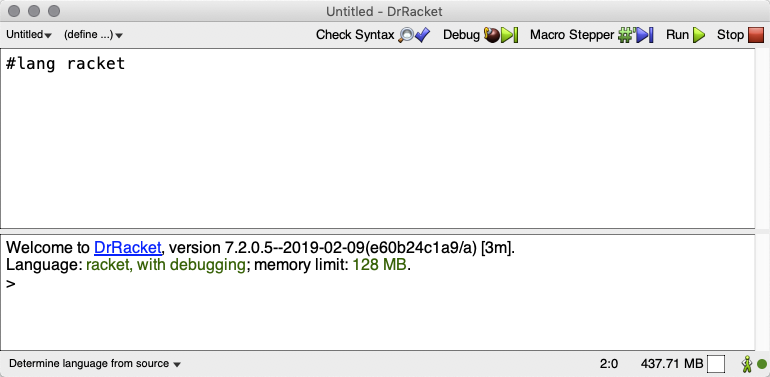
\includegraphics[width=\textwidth]{i1prog/drracket-start}
  \caption{DrRacket nach dem ersten Start}
  \label{fig:drracket-start}
\end{figure}

Zu Racket gehört ein Programm namens
\textit{DrRacket}\index{DrRacket}: starte es.  Es erscheint ein
Fenster, das ungefähr so aussehen sollte wie in
Abbildung~\ref{fig:drracket-start}.  Die Benutzeroberfläche kannst
Du auf Deutsch umstellen, indem Du im Hilfe-Menü auf \texttt{Deutsche
  Benutzeroberfläche für DrRacket} drückst.  Wenn Du die Auswahl
bestätigst, wird DrRacket danach beendet und Du musst es noch einmal
starten; dann sollten die Menüs auf Deutsch sein.

DrRacket ist eine \textit{Entwicklungsumgebung}, mit der Du Programme
schreiben und ausführen kannst.  DrRacket unterstützt nicht nur eine
Programmiersprache, darum musst Du die richtige Programmiersprache für
dieses Buch noch auswählen.  Dazu wählst Du den Menüpunkt
\texttt{Sprache $\rightarrow$ Sprache auswählen} (bzw.\
\texttt{Language $\rightarrow$ Choose language} in der englischen
Fassung), worauf ein Dialog erscheint.  In dem Dialog gibt es eine
Abteilung \texttt{Lehrsprachen\index{Lehrsprachen}}, und darunter eine
Überschrift namens \texttt{DeinProgramm}, unterhalb dessen mehrere
Einträge erscheinen, die speziell auf die Kapitel dieses Buchs
zugeschnitten sind.

\begin{figure}[tb]
  \centering
  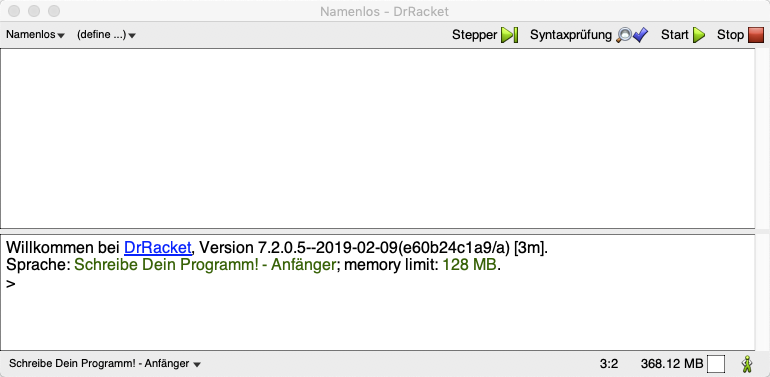
\includegraphics[width=\textwidth]{i1prog/drracket-deinprogramm}
  \caption{DrRacket mit ausgewählter Lehrsprache}
  \label{fig:drracket-deinprogramm}
\end{figure}

Für den ersten Teil des Buches ist die Ebene \texttt{Schreibe Dein
  Programm! - Anfänger} zuständig:\index{Sprachebene!Anfänger} Wähle
diese aus und drücke dann einmal oben rechts auf den Knopf
\texttt{Start} (bzw.\ \texttt{Run}), damit die Auswahl aktiv wird.
Das Ergebnis sollte dann so aussehen wie in
Abbildung~\ref{fig:drracket-deinprogramm}.

Das DrRacket-Fenster besteht aus zwei Teilen:
%
\begin{enumerate}
\item In der oberen Hälfte des Fensters (dem
  \textit{Editor\index{Editor}} oder
  \textit{Definitionsfenster\index{Definitionsfenster}}) steht der
  Programmtext.  Der Editor funktioniert ähnlich wie ein reguläres
  Textverarbeitungsprogramm.  Was dort steht, kannst Du abspeichern.
\item In der unteren Hälfte des Fensters~-- dem
  \textit{Interaktionsfenster\index{Interaktionsfenster}} oder der
  sogenannten \textit{REPL\index{REPL}}\footnote{"`REPL"' steht für
    "`Read-Eval-Print-Loop"'~-- wir werden später zeigen, warum.}
  werden die Ausgaben des Programms angezeigt.  Außerdem kannst Du
  hier "`Fragen"' an das Programm stellen, um einzelne Programmteile
  gezielt auszuprobieren.
\end{enumerate}
%

\section{Ausdrücke und die REPL}

Fangen wir mit der REPL an: Wenn Du gerade \texttt{Start} gedrückt
hast, dann erscheint der Cursor rechts von dem \verb|>|-Zeichen: Du
kannst da etwas eingeben und Return drücken~-- DrRacket zeigt dann
das Ergebnis darunter an.

Wenn Du zum Beispiel \texttt{123} eintippst, zeigt DrRacket gleich
darunter 123 an.  DrRacket kann auch rechnen.  Dafür musst Du
allerdings die Rechenaufgaben etwas anders aufschreiben als sonst.
Zum Beispiel so:
%
\begin{verbatim}
(+ 123 42)
\end{verbatim}
%
Wenn Du das in die REPL tippst, zeigt DrRacket \texttt{165} an, die
\textit{Summe}\index{Summe} von 123 und 42.  Diese "`Rechenaufgabe"'
ist ein sogenannter \textit{Ausdruck\index{Ausdruck}}.  Ausdrücke, die
etwas ausrechnen sollten, haben in den Lehrsprachen immer die gleiche
Form, und die sieht so aus:
%
\begin{alltt}
(\textnormal{\textit{Operator}} \textnormal{\textit{Operand}} \ldots)
\end{alltt}
%
Das heißt, da stehen \emph{immer} Klammern\index{Klammer} drumherum
(und die können auch nirgendwo sonst stehen).  Dann steht da der
\textit{Operator\index{Operator}}, der bestimmt, \emph{was} gemacht
wird, also die \textit{Operation}.  Danach kommen die
\textit{Operanden\index{Operand}}, welche die Eingaben\index{Eingabe}
für die Operation bestimmen.

Zum Merken ist es hilfreich, Ausdrücke entsprechend vorzulesen: Also
nicht mehr "`Hundertdreiundzwanzig plus zweiundvierzig"', sondern
"`die \emph{Summe} von Hundertdreiundzwanzig und zweiundvierzig"'.

Wie schon gesagt, die Klammern sind wichtig.  Wenn Du sie vergisst,
können verwirrende Ergebnisse herauskommen.  Wenn Du zum Beispiel
\texttt{+ 123 42} in der REPL eintippst, sieht das so aus:
%
\begin{alltt}
> + {\color{green}123 42}
{\color{blue}#<function:+>
123
42}
\end{alltt}
%
Das liegt daran, dass ohne Klammern \texttt{+ 123 32} aus \emph{drei}
Ausdrücken besteht und die REPL darum auch drei Ergebnisse ausdruckt:
Die Funktion \texttt{+}, dann die \texttt{123}, dann \texttt{42}.
(Die Operation \texttt{+} ist eine sogenannte Funktion ist~-- das
erläutern wir später noch genauer.)  Ähnlich verhält es sich mit
\texttt{123 + 42}~-- probiere es aus!

Wenn Du versehentlich den Operator dazwischen schreibst, erscheint
in der REPL eine Fehlermeldung:
%
\begin{alltt}
> ({\color{green}123} + {\color{green}42})
{\color{red}Operator darf keine Zahl sein, ist aber 123}
\end{alltt}
%
Etwas ähnliches passiert, wenn Du kein Leerzeichen zwischen den
Operator und die Operanden oder zwischen die Operanden setzt.  Das
sieht zum Beispiel so aus:
%
\begin{alltt}
> ({\color{green}+123} {\color{green}42})
{\color{red}Operator darf keine Zahl sein, ist aber 123}
\end{alltt}
%
Das liegt daran, dass \texttt{+123} zusammen die Zahl "`plus
hundertdreiundzwanzig"' bildet und nicht etwa in das \texttt{+} und
\texttt{123} aufgeteilt wird.

Wenn ein Ausdruck wie \texttt{(+ 123 42)} ein Ergebnis wie 165 hat,
schreiben wir das im Buch zukünftig so, etwas anders als die
DrRacket-REPL:
%
\begin{alltt}
(+ 123 42)
\evalsto{} 165
\end{alltt}
%
Es gehen natürlich nicht nur Summen, sonderen auch Differenzen,
Produkte und Quotienten:
%
\begin{alltt}
(- 123 42)
\evalsto{} 81
(* 123 42)
\evalsto{} 5166
(/ 123 42)
\evalsto{} 2.9\(\overline{\mathtt{285714}}\)
\end{alltt}
%
Beim letzen Ausdruck ist zu sehen, dass Dezimalzahlen mit Punkt und
nicht mit Komma geschrieben werden.  Der Überstrich bei
\texttt{2.9\(\overline{\mathtt{285714}}\)} ist eine
\textit{Periode\index{Periode}}. Die Zahl ist also eigentlich
%
\begin{alltt}
2.9285714285714285714285714285714\ldots
\end{alltt}
%
Die REPL funktioniert also folgendermaßen: Sie \emph{liest} einen
Ausdruck ein ("`read"'), berechnet deren Wert oder \emph{wertet}
diesen \emph{aus} (auf Englisch "`eval"') und zeigt das Ergebnis an
oder \emph{druckt} dieses \emph{aus} ("`print"')~-- und dann geht es
von vorn los, wie in einer Schleife ("`loop"').  Die Abfolge
\emph{Read-Eval-Print-Loop} gibt der REPL ihren Namen.

Ausdrücke können auch kombiniert werden, zum Beispiel so:
%
\begin{alltt}
(* 123 (+ 20 22))
\evalsto{} 5166
(* 123 (+ (* 2 10) 22))
\evalsto{} 5166
\end{alltt}
%
Bei der Kombination ist wichtig, dass um jeden Teilausdruck wieder ein
Klammernpaar kommt.  Ist das nicht der Fall, erscheinen gelegentlich
auch mal englischsprachige Fehlermeldungen wie diese hier:
%
\begin{alltt}
(* 123 (+ * 2 10 22))
{\color{red}+: expects a number as 1st argument, given #<function:*>}
\end{alltt}
%
Das liegt daran, dass das \texttt{*} hier an der Stelle eines
Operanden für die Summe dient.  Ein anderes Wort für Operand in diesem
Zusammenhang ist \textit{Argument}, darum steht da sinngemäß, dass
\texttt{+} eine Zahl als erstes Argument etwartet, aber
stattdessen die Funktion \texttt{+} bekommen hat.

Ein hilfreicher Trick übrigens: Um einen Ausdruck zu korrigieren,
kannst Du ihn in der REPL "`zurückholen"', indem Du \texttt{Esc}, und
dann \texttt{P} drückst~-- probier es aus!

\begin{aufgabe}
  Schreibe folgende "`mathematischen"' Ausdrücke in der Notation der
  Lehrsprache in die REPL und lasse die REPL sie auswerten:
  %
  \begin{displaymath}
    \begin{array}{c}
      55 * 27\\
      23 * (44 + 27)\\
      \frac{23}{44} + \frac{44}{23}\\
      (23 + 42) * (12 + (14 * 2))
    \end{array}
  \end{displaymath}
\end{aufgabe}
%
Ein weiterer praktischer Trick ist, dass Du einen geklammerten
Ausdruck markieren (und dann ausschneiden) kannst, indem Du auf die
öffnende oder schließende Klammer doppelt klickst.

\section{Das Definitionsfenster}

Kommen wir zum Definitionsfenster oben.  Dort schreibst Du Dein
Programm, die REPL kannst Du dann benutzen, um es auszuprobieren.
Schreib in das Definitionsfenster folgende
\textit{Definition\index{Definition}}:
%
\begin{verbatim}
(define alles (+ 20 22))
\end{verbatim}
%
Diese Definition besagt, dass der Name \texttt{alles} für das Ergebnis
von \texttt{(+ 20 22)} steht.  Um das auszuprobieren, drück auf den
Knopf \texttt{Start} bzw.\ \texttt{Run} rechts oben.  Der Cursor
landet dann wieder in der REPL, wo Du das Programm ausprobieren
kannst:
%
\begin{alltt}
alles
\evalsto{} 42
\end{alltt}
%
Ein Name, der in einem Programm so definiert ist, heißt
\textit{Variable\index{Variable}}.

Hier sind ein paar weitere Beispiele für Definitionen:
%
\begin{alltt}
(define one 1)
(define temperature 23)
(define birgit-prinz 9)
(define michael-ballack 13)
\end{alltt}
%
Bei der Gestaltung eines Namens gibt es weitgehende
Freiheiten.\footnote{Anders als in anderen Programmiersprachen sind
  auch Bindestriche in Namen möglich.}  Nur Leerzeichen sind nicht
erlaubt.

In einem Programm kannst Du Zeilenumbrüche und Einrückung benutzen, um
Dein Programm übersichtlicher zu gestalten.  Zum Beispiel kannst Du
nach \texttt{alles} die Return-Taste drücken, das Ergebnis sieht so
aus:
%
\begin{alltt}
(define alles
  (+ 20 22))
\end{alltt}
%
DrRacket rückt die zweite Zeile ein bisschen ein, um auszudrücken,
dass sie noch in die Klammern vom \texttt{define} gehört.  Bei
komplizierteren Ausdrücken ist das hilfreich:
%
\begin{verbatim}
(define alles
  (+ 20
     (* 11 2)))
\end{verbatim}
%
Hier stellt DrRacket die Operanden der Summe genau untereinander.
DrRacket zwingt Dich nicht, die Einrückung genau so zu machen, und
durch Änderungen im Programm gerät sie auch manchmal aus dem Lot.  In
dem Fall kannst Du die Tab-Taste drücken (auf den meisten Tastaturen
steht $\longrightarrow\mid$ auf der Tab-Taste) und in der Zeile, in
welcher der Cursor steht, wird die Einrückung korrigiert.  Es gibt
einen Menüpunkt \texttt{Racket $\rightarrow$ Alles einrücken} (bzw.\
\texttt{Racket $\rightarrow$ Reindent All}), der das für das gesamte
Programm macht: Probier es aus!

\begin{aufgabe}
  Bring bei einem mehrzahligen Programm die Einrückung richtig
  durcheinander, zum Beispiel so:
\begin{verbatim}
(define nr
  (+ 12
 (- (* 42
  13)
    500)))
\end{verbatim}
  %
  Benutze dann die Tab-Taste, um die Einrückung wieder zu korrigieren.
\end{aufgabe}
%
Den Inhalt des Definitionsfenster kannst Du abspeichern, indem Du auf
den Knopf mit der Diskette
\raisebox{-1ex}{
\includegraphics[height=12pt]{i1prog/save}} drückst.

Abspeichern geht mit der REPL nicht, und der REPL-Inhalt verschwindet
auch jedesmal, wenn Du \texttt{Start} bzw.\ \texttt{Run} drückst.  Du
kannst aber frühere Eingaben zurückholen, indem Du \texttt{Esc~P}
drückst.

\section{Rechnen ohne Zahlen}

Computerprogramme können nicht nur mit Zahlen rechnen.  In diesem
Abschnitt geht es um das Rechnen mit Text und das Rechnen mit Bildern.

\subsection{Rechnen mit Zeichenketten}

Zum Beispiel gibt es auch Text, der in einem Programm immer von
doppelten Anführungszeichen umschlossen ist, zum Beispiel:
%
\begin{alltt}
"Mike Sperber"
"Herbert Klaeren"
"Schreibe Dein Programm!"
\end{alltt}
%
Diese Werte heißen \textit{Zeichenketten\index{Zeichenkette}}.

Die einfachste Art, eine Zeichenkette herzustellen, ist, die
Buchstaben hinzuschreiben, aus denen sie besteht.  Die
Anführungszeichen müssen drumherum, um die Zeichenketten von anderen
Ausdrücken zu unterscheiden.  Die Anführungszeichen gehören aber nicht
zu den Buchstaben dazu, aus denen die Zeichenkette besteht~--
\verb|"abc"| besteht aus den drei Buchstaben \texttt{abc}.

\begin{feature}{Zeichenketten}{scheme:strings}
\textit{Zeichenketten\index{Zeichenkette}} (auf Englisch
\textit{Strings}\index{String}) repräsentieren Text.
Literale für Zeichenketten haben folgende Form:
%
\begin{alltt}
"\(z\sb{1}\)\(z\sb{2}\) \(\ldots\) \(z\sb{n}\)"
\end{alltt}
%
Dabei sind die \(z\sb{i}\) beliebige einzelne Zeichen, außer \verb|"| selbst.
Beispiel:
%
\begin{alltt}
"Herbert was here!"
\end{alltt}
%
Das Anführungszeichen (\verb|"|) kann nicht "`ungeschützt"' vorkommen, da es das Ende der
Zeichenkette markiert. Es wird als Zeichen innerhalb einer Zeichenkette
durch \verb|\"| dargestellt:
%
\begin{alltt}
"Herbert sagt, Mike wäre \backwhack{}"doof\backwhack{}"!"
\end{alltt}
\end{feature}

Abbildung~\ref{scheme:strings} beschreibt die genaue Schreibweise für
solche "`festen"' Zeichenketten.  Feste Schreibweisen für Werte heißen
allgemein \textit{Literale\index{Literal}}.  Das kennen wir schon von
den Zahlen: Die Zeichenfolge \texttt{123} steht für die Zahl
"`hundertdreiundzwanzig"'.  Kästen wie Abbildung~\ref{scheme:strings}
werden in diesem Buch noch oft dazu dienen, neue Sprachelemente
einzuführen.

Mit Text kann ein Programm auch rechnen, und zwar mit der eingebauten
Funktion
\texttt{string"=append}\index{string-append@\texttt{string-append}},
die zwei Zeichenketten aneinanderhängt:
%
\begin{alltt}
(string-append "Herbert" "Mike")
\evalsto{} "HerbertMike"
(string-append "Mike" " " "ist doof")
\evalsto{} "Mike ist doof"
\end{alltt}
%
Die eingebaute Funktion
\texttt{string-length}\index{string-length@\texttt{string-length}}
liefert die Anzahl der Buchstaben in einer Zeichenkette:
%
\begin{alltt}
(string-length "Herbert")
\evalsto{} 7
(string-length "Mike")
\evalsto{} 4
\end{alltt}
%
Die Namen \texttt{string-append} und \texttt{string-length} sehen auf
den ersten Blick "`anders"' aus als \texttt{+} und \texttt{*} zum
Beispiel, dieser Eindruck täuscht jedoch: Sie sind allesamt Namen von
vordefinierten Operationen, die Programme benutzen können, ohne sie
selbst definieren zu müssen.

Die vordefinierten Funktionen
\texttt{string->number}\index{string->number@\texttt{string->number}}
und \texttt{number->string} konvertieren zwischen Zahlen und den
Zeichenketten, die diese darstellen:
%
\begin{alltt}
(string->number "23")
\evalsto{} 23
(number->string 23)
\evalsto{} "23"
\end{alltt}
%
\begin{aufgabe}
  Mache Dir den Unterschied zwischen der Zahl \texttt{23} und der
  Zeichenkette \verb|"23"| klar.  Probiere zum Beispiel aus:
\begin{alltt}
(+ "23" 42)
(string-append 23 "42")
(number->string "23")
\end{alltt}
\end{aufgabe}

\subsection{Rechnen mit Bildern}

Programme können auch mit Bildern rechnen.  Dazu wird eine Erweiterung
zu DrRacket benötigt, ein sogenanntes
\textit{Teachpack}\index{Teachpack}: Wähle dazu den Menüpunkt
\texttt{Sprache $\rightarrow$ Teachpack hinzufügen}.  (Beziehungsweise
\texttt{Language $\rightarrow$ Add Teachpack}.  In dem Dialog, der
dann erscheint, wähle \texttt{image.rkt} aus und drücke dann
\texttt{OK}.  Dann musst Du noch einmal auf \texttt{Start} drücken.

Das Teachpack \texttt{image.rkt} enthält zusätzliche vordefinierte
Funktionen, mit denen wir Bilder herstellen können.  Zum Beispiel
\texttt{square}, \texttt{circle} und \texttt{star-polygon}:
%
\begin{alltt}
(square 40 "solid" "red")
\evalsto{} 
\includegraphics[height=24pt]{i1prog/square}
(circle 40 "solid" "green")
\evalsto{} 
\includegraphics[height=24pt]{i1prog/circle}
(star-polygon 20 10 3 "solid" "blue")
\evalsto{} 
\includegraphics[height=24pt]{i1prog/starpolygon}
\end{alltt}
%
Schauen wir uns das eingebaute \texttt{star-polygon} etwas näher an:
Es akzeptiert fünf Eingaben, die ersten drei davon sind Zahlen~-- die
Seitenlänge, die Seitenanzahl und die Anzahl der Ecken, die für jede
Seite übersprungen wird.  Danach kommen zwei Zeichenketten~--
\verb|"solid"| heißt, dass das Innere des Sterns ausgefüllt ist und
\verb|"blue"| ist die Farbe.  Statt \verb|"solid"| kannst Du auch
\verb|"outline"| schreiben, dann wird auch etwas klarer, was
"`überspringen"' heißt:
%
% filename can't contain hyphen because of alltt
\begin{alltt}
(star-polygon 20 10 3 "outline" "blue")
\evalsto{} 
\includegraphics[height=24pt]{i1prog/starpolygon_outline}
\end{alltt}
%
\begin{aufgabe}
  Wofür stehen die Zahleneingaben bei \texttt{square} und
  \texttt{circle}?  Probiere unterschiedliche Zahlen aus!  Es gibt
  auch eine eingebaute Funktion \texttt{rectangle}.  Kannst Du ein
  funktionierendes Beispiel für den Einsatz von \texttt{rectangle}
  konstruieren?  Außerdem gibt es eine eingebaute Funktion
  \texttt{ellipse}, die genauso benutzt wird wie \texttt{rectangle}~--
  probiere sie aus!
\end{aufgabe}
%
Bilder sind Werte wie Zahlen und Zeichenketten auch.  Du kannst
mit Definitionen auch Namen dafür vergeben:
%
\begin{verbatim}
(define s1 (square 40 "solid" "red"))
(define c1 (circle 40 "solid" "green"))
(define p1 (star-polygon 20 10 3 "solid" "blue"))
\end{verbatim}
%
\begin{aufgabe}
  Du kannst auch Bilddateien oder Bilder in Webseiten in Dein Programm
  einfügen, wie in einem Textverarbeitsprogramm.  Probier es aus und
  gib dem Bild einen Namen!
\end{aufgabe}

%
Mit Bildern kann DrRacket auch rechnen:
%
\begin{alltt}
(beside s1 p1)
\evalsto{} 
\includegraphics[height=24pt]{i1prog/beside.png}
(above s1 c1)
\evalsto{} 
\includegraphics[width=24pt]{i1prog/above.png}
(above (beside s1 p1) (beside p1 c1))
\evalsto{} 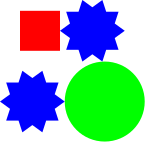
\includegraphics[width=48pt]{i1prog/abovebeside.png}
\end{alltt}
%
FIXME: Haus aus Dreieck und Quadrat

Das heißt, \texttt{beside} akzeptiert als Eingabe zwei (oder mehr)
Bilder und macht daraus wieder ein Bild, in dem die Teilbilder
nebeneinander stehen.  Das gleiche gilt für \texttt{above}, nur dass
die Bilder übereinander angeordnet werden.  Selbstverständlich können
\texttt{above} und \texttt{beside} auch kombiniert werden.

\section{Abstraktion und Applikation}
\label{sec:abstraktion-und-applikation}

Hier sind zwei Ausdrücke, welche die Bilder aus dem vorigen Abschnitt
zu einem Muster kombinieren:
%
\begin{alltt}
(above
 (beside s1 p1)
 (beside p1 s1))
\evalsto{} 
\includegraphics[width=48pt]{i1prog/tile1}

(above
 (beside p1 c1)
 (beside c1 p1))
\evalsto{} 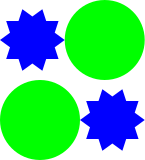
\includegraphics[width=48pt]{i1prog/tile2}
\end{alltt}
%
Beide Ausdrücke folgen dem gleichen Muster, sie "`kacheln"' jeweils zwei
Bilder in einer quadratischen Anordnung.  Das Muster könnte man so
hinschreiben:
%
\begin{verbatim}
(above
 (beside a b)
 (beside b a))
\end{verbatim}
%
Das erste Beispiel entsteht dann, indem für \texttt{a} \texttt{s1}
eingesetzt wird und für \texttt{b} \texttt{p1}, im zweiten für \texttt{a}
\texttt{p1} und für \texttt{b} dann \texttt{c1}.

Dieses Muster kannst Du in ein Programm gießen.  Dann müssen wir nicht
jedesmal \texttt{above \ldots{} beside \ldots{} beside} eintippen.
Dazu schreibst Du es erst einmal genauso hin, also mit \texttt{a} und
\texttt{b}.  Wenn Du das Programm startet, erscheint folgende Meldung:
%
\begin{alltt}
\color{red}a: Ungebundene Variable
\end{alltt}
%
Na klar, es gibt ja auch keine Definition für \texttt{a}.  Du könntest
eine hinschreiben, zum Beispiel:
%
\begin{verbatim}
(define a s1)
\end{verbatim}
%
Aber dann wäre \texttt{a} auf \texttt{s1} festgelegt.  Wir wollen
stattdessen das Muster verallgemeinern, so dass Du es mehrmals mit
unterschiedlichen Werten für \texttt{a} und \texttt{b} verwenden
kannst.  Dieser Verallgemeinerungsprozess heißt beim Programmieren
\textit{Abstraktion\index{Abstraktion}}.  Dafür müssen wir dem Muster
noch etwas hinzufügen, um zu sagen, dass wir unterschiedliche Werte
für \texttt{a} und \texttt{b} einsetzen wollen:
%
\begin{verbatim}
(lambda (a b)
  (above
   (beside a b)
   (beside b a)))
\end{verbatim}
%
Die \texttt{lambda}\index{lambda@\texttt{lambda}} ist eine Art Zauberwort, es sagt soviel wie: "`Für
die Variablen \texttt{a} und \texttt{b} möchte ich später (und
vielleicht mehrmals) Werte einsetzen."'  Wenn Du das Programm jetzt
startest, geht die Fehlermeldung weg und in der REPL erscheint:
%
\begin{alltt}
#<function:\ldots>
\end{alltt}
%
(Der Text anstelle des \ldots{} variiert etwas von Fall zu Fall.)

Das deutet darauf hin, dass bei dem \texttt{lambda} eine Funktion
herauskommt.  Um etwas damit anfzufangen, gib ihr einen Namen mit
\texttt{define}:
%
\begin{verbatim}
(define tile
  (lambda (a b)
    (above
     (beside a b)
     (beside b a))))
\end{verbatim}
%
(Alles schön richtig einrücken! "`Tile"' heißt auf Deutsch
"`kacheln"'.)

Dadurch ist eine neue Operation entstanden.  Die kannst Du direkt
verwenden:
%
\begin{alltt}
(tile s1 p1)
\evalsto{} 
\includegraphics[width=48pt]{i1prog/tile1}

(tile p1 c1)
\evalsto{} 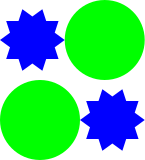
\includegraphics[width=48pt]{i1prog/tile2}
\end{alltt}
%
Was ist da passiert?  Am einfachsten kann man das in einem speziellen
Werkzeug sehen, dem \textit{Stepper\index{Stepper}}.  Um ihn zum
Einsatz zu bringen, sorge dafür, dass im Definitionsfenster folgendes
Programm steht, also das, was weiter oben schon steht:
%
\begin{verbatim}
(define s1 (square 40 "solid" "red"))
(define c1 (circle 40 "solid" "green"))
(define p1 (star-polygon 20 10 3 "solid" "blue"))

(define tile
  (lambda (a b)
    (above
     (beside a b)
     (beside b a))))

(tile s1 p1)
(tile p1 c1)
\end{verbatim}
%
Dann drück auf den \texttt{Stepper}-Knopf oben rechts im
DrRacket-Fenster.  Es erscheint ein neues Fenster, das so aussieht:

\begin{figure}[H]
  \centering
  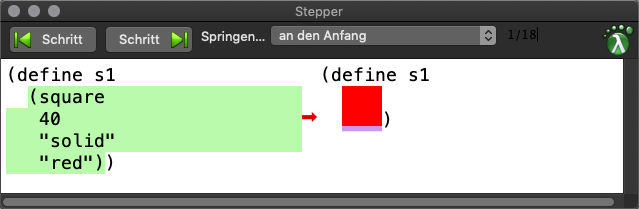
\includegraphics[width=0.6\textwidth]{i1prog/stepper-0}
  \caption{Der Stepper in Aktion}
  \label{fig:stepper-0}
\end{figure}
%
\noindent Du kannst jetzt mit den Knöpfen mit dem Vorwärts- beziehungsweise dem
Rückwärts-Pfeil zusehen, wie DrRacket Dein Programm ausführt.  Wenn Du
ein paar Schritte vorwärts gehst, sieht das so aus:
%
\begin{figure}[H]
  \centering
  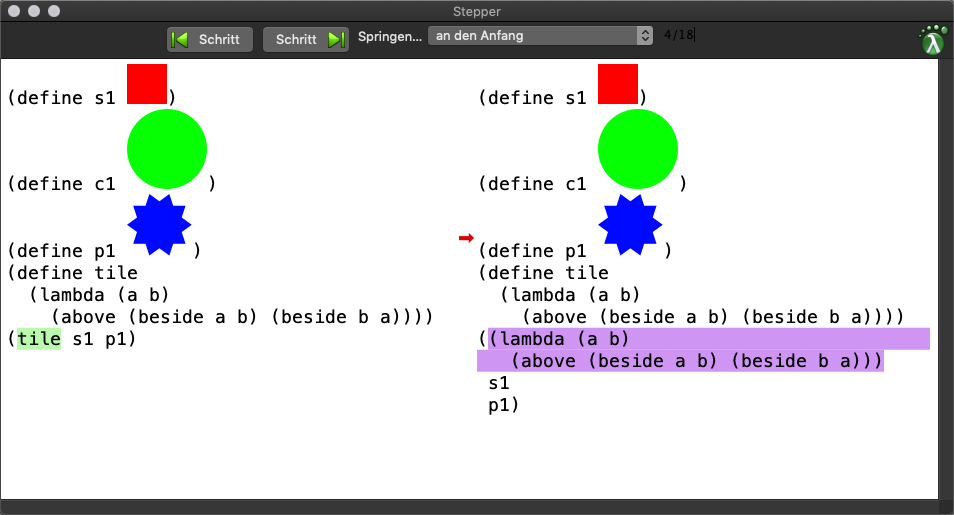
\includegraphics[width=0.8\textwidth]{i1prog/stepper-1}
  \caption{Stepper: Variable ersetzen}
  \label{fig:stepper-1}
\end{figure}
%
\noindent Du kannst sehen, wie DrRacket jeweils einen Ausdruck einen Schritt auf
einmal auswertet~-- der ist auf der linken Seite grün~-- und dann
rechts durch das Resultat ersetzt.  Oben kannst Du sehen, wie der
Stepper die Variable \texttt{tile} durch den \texttt{lambda}-Ausdruck
aus der Definition von \texttt{tile} ersetzt. Das macht der Stepper
auch mit den Definitionen von \texttt{s1} und \texttt{p1}:
%
\begin{figure}[H]
  \centering
  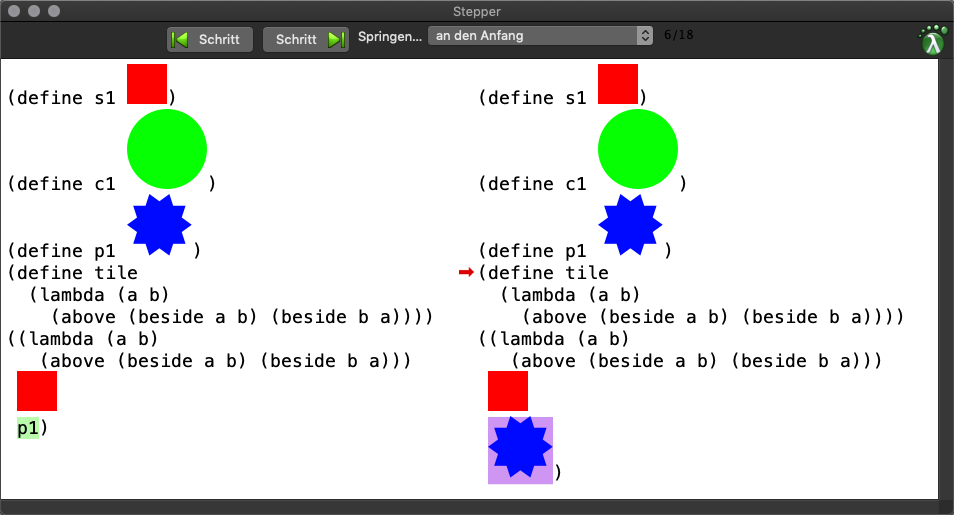
\includegraphics[width=0.8\textwidth]{i1prog/stepper-2}
  \caption{Stepper: Variable}
  \label{fig:stepper-2}
\end{figure}
%
\noindent Interessant wird es danach. Die Variablen aus den Definitionen sind
alle ersetzt.  Hinter dem \texttt{lambda}-Ausdruck stehen jetzt das
Quadrat und der Stern, und die werden jetzt für die Variablen aus dem
\texttt{lambda}-Ausdruck eingesetzt, also das Quadrat für \texttt{a}
und der Stern für \texttt{b}:
%
\begin{figure}[H]
  \centering
  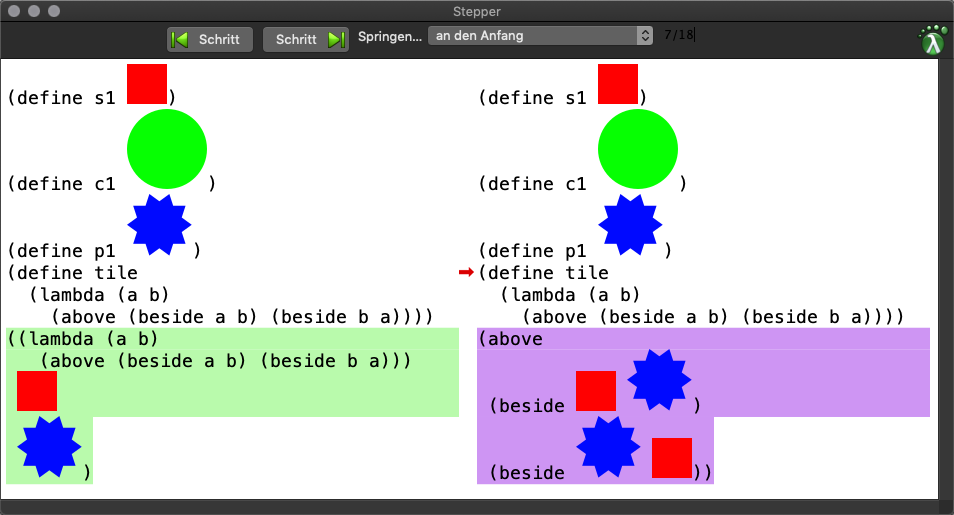
\includegraphics[width=0.8\textwidth]{i1prog/stepper-3}
  \caption{Stepper: Applikation}
  \label{fig:stepper-3}
\end{figure}
%
\noindent Dabei verschwindet auch das \texttt{lambda}.
%
\begin{aufgabe}
  Probiere das Beispiel im Stepper aus und klicke Dich bis zum Ende
  durch. Mache Dir dabei klar, wie jeweils die linke mit der rechten
  Seite zusammenhängt.
\end{aufgabe}
%
\texttt{(tile s1 p1)} ist eine sogenannte
\textit{Applikation\index{Applikation}}: Das ist ein Ausdruck mit
(natürlich) Klammern drum.  Der Operator und die Operanden der
Applikation sind ebenfalls Ausdrücke.  Der Operator ergibt eine
Funktion~-- entweder eingebaut oder aus einem
\texttt{lambda}-Ausdruck.

Wenn die Funktion ein \texttt{lambda}-Ausdruck ist wie in
Abbildung~\ref{fig:stepper-3}, dann muss es genauso viele Operanden
geben wie der \texttt{lambda}-Ausdruck Variablen hat.
Dann wertet DrRacket den Ausdruck wie folgt aus:
%
\begin{enumerate}
\item Die Operanden werden ausgewertet und ergeben die sogenannten
  \textit{Argumente\index{Argument}}.
\item Die Argumente werden ausgewertet und die Ergebnisse für die
  Variablen des \texttt{lambda}-Ausdrucks~-- die sogenannten
  \textit{Parameter\index{Parameter}}~-- im Innenteil des
  \texttt{lambda}-Ausdrucks, dem \textit{Rumpf\index{Rumpf}}
  eingesetzt.
\end{enumerate}
%
\begin{feature}{Abstraktion und Applikation}{scheme:abstraction}
  Eine Abstraktion\index{Abstraktion} hat folgende Form:
\begin{alltt}
(lambda (\(p\sb{1} \ldots p\sb{n}\)) \(e\))
\end{alltt}
  %
  Die $p_i$ sind jeweils Namen, die \textit{Parameter}\index{Parameter}, und
  $e$ ist der \textit{Rumpf}\index{Rumpf}.  In $e$ dürfen die $p_i$
  vorkommen.  Der Wert einer Abstraktion ist eine \textit{Funktion}\index{Funktion},
  welche für jeden Parameter eine Eingabe erwartet.

  Eine \textit{Applikation} einer Funktion hat folgende Form:
  %
\begin{alltt}
(\(p\) \(a\sb{1}\) \ldots \(a\sb{n}\))
\end{alltt}
  %
  $p$ ist ein Ausdruck, der eine Funktion ergeben muß, die $a_i$ sind
  ebenfalls Ausdrücke, die \textit{Argumente}\index{Argument}.  Bei
  der Auswertung einer Applikation werden zunächst $p$ und die $a_i$
  ausgewertet; danach geht es mit der Auswertung des Rumpfes der
  Funktion weiter, wobei für die Parameter $p_i$ jeweils die Werte der
  Argumente $a_i$ eingesetzt werden.
\end{feature}
%
\texttt{Lambda}-Ausdrücke heißen auch
\textit{Abstraktionen\index{Abstraktion}}.
Abbildung~\ref{scheme:abstraction} fasst zusammen, wie Abstraktionen
und Applikationen aufgebaut sind und ausgewertet werden.

Verwirrend ist vielleicht der Unterschied zwischen Abstraktion und
Funktion: Die Abstraktion ist der \texttt{lambda}-Ausdruck im
Programm, die Funktion ist der Wert, der bei der Programmauswertung
dabei herauskommt.  Wir verwenden im Buch aber häufig den Begriff
"`Funktion"' für eine Abstraktion, weil uns interessiert, was bei der
Abstraktion herauskommt.

\begin{aufgabe}
  Denke Dir ein einzelnes Muster aus, mit dem mehrere Bilder
  kombiniert werden können (es muss nichts kompliziertes sein) und
  schreibe eine Funktion, die dies erledigt: Benutze diese Funktion,
  um mehrere Sätze von Bildern zu kombinieren.
\end{aufgabe}

\section{Exkurs: Information und Daten}

Eine Definition wie
%
\begin{alltt}
(define mehrwertsteuer 19)
\end{alltt}
%
suggeriert, dass die Zahl 19 an dieser Stelle eine Bedeutung "`in der
realen Welt"' hat, zum Beispiel in einem Programm, das eine Registrierkasse
steuert oder das bei der Steuererklärung hilft.  Die Bedeutung könnte
folgende Aussage sein: "`Der Mehrwertsteuersatz beträgt 19\%."'
Dieser Satz repräsentiert \textit{Information}\index{Information},
also einen Fakt über die Welt oder zumindest den Ausschnitt der Welt, in
dem das Programm arbeiten soll.  In Computerprogrammen wird
Information in eine vereinfachte Form gebracht, mit der das Programm
rechnen kann~-- in diesem Fall die Zahl 19.  Diese vereinfachte Form
heißt \textit{Daten}\index{Daten}: Daten sind
\textit{Repräsentationen}\index{Repräsentation} für Information.

Eine der wichtigsten Aufgaben beim Programmieren ist, die richtigen
Form für die Daten zu wählen, um die für das Programm relevanten
Informationen darzustellen die Informationen dann in Daten zu
übersetzen.

Nicht immer ist offensichtlich, welche Information durch bestimmte
Daten repräsentiert werden.  Die Zahl 23 zum Beispiel könnte eine Reihe
von Informationen darstellen:
%
\begin{itemize}
\item die Anzahl der Haare von Bruce Willis
\item die aktuelle Außentemperatur in °C in Tübingen
\item die Außentemperatur vom 1.7.2000 in °C in Tübingen
\item die Größe in m$^2$ des Schlafzimmers
\item die Rückennummer von Alexandra Popp
\end{itemize}
%
Damit andere unsere Programme lesen können, werden wir also immer
wieder klarstellen müssen, wie Information in Daten zu übersetzen ist
und umgekehrt.

\section{Programme systematisch konstruieren}

In Abschnitt~\ref{sec:abstraktion-und-applikation} haben wir gezeigt,
wie Abstraktion und Applikation bei der Programmauswertung
funktionieren.  Das Verständnis dafür ist wichtig, aber Du musst beim
Schreiben Deines Programms nicht die ganze Zeit daran denken, wie
DrRacket Dein Programm auswertet.  Entsprechend kümmern wir uns in
diesem Buch hauptsächlich darum, wie Du Programme systematisch
konstruierst.
Schauen wir uns das anhand einer realistischen Aufgabe an:
%
\begin{aufgabe}
  \label{aufgabe:stromtarif}
  Betrachte folgende Stromtarife.  Beide Tarife
  bestehen aus einer monatlichen Grundgebühr und einem Teil, der sich
  nach den verbrauchten Kilowattstunden (kWh) richtet.
  %
  \begin{center}
    \begin{tabular}{l|c|c|}
      & Grundgebühr pro Monat & Verbrauchspreis pro kWh \\
      \hline
      Tarif "`Billig-Strom"' & \EUR{4,90} & \EUR{0.19} \\
      \hline
      Tarif "`Watt für wenig"' & \EUR{8,20} & \EUR{0.16} \\
      \hline
    \end{tabular}
  \end{center}

  \begin{enumerate}
  \item Schreibe ein Programm das den Monatsverbrauch in
    Kilowattstunden akzeptiert und den im Tarif "`Billig-Strom"' zu
    zahlenden monatlichen Rechnungsbetrag berechnet.

  \item Schreibe ein Programm, die den Monatsverbrauch in
    Kilowattstunden akzeptiert und den im Tarif "`Watt für wenig"' zu
    zahlenden monatlichen Rechnungsbetrag
    berechnet.
  \end{enumerate}
  %
\end{aufgabe}
%
Fangen wir mit dem ersten Aufgabenteil an!

\paragraph{Funktion}

Zunächst einmal: Da steht "`Schreibe ein Programm~\ldots"'.  In den
Lehrsprachen dieses Buchs heißt das immer "`Schreibe eine
\emph{Funktion}~\ldots"'.  Später werden wir Programme schreiben, die
neben der "`Hauptfunktion"' noch "`Hilfsfunktionen"' haben, aber das
Prinzip bleibt immer das gleiche.

Wenn dort steht, "`das den Monatsverbrauch in Kilowattstunden
akzeptiert"', dann bedeutet dies, dass die Funktion den
Monatsverbraucht als Eingabe akzeptieren soll~-- also als Argument.

Ebenso bedeutet "`und den \ldots{} zu zahlenden monatlichen
Rechnungsbetrag berechnet"', dass die Funktion diesen Rechungsbetrag
als Ergebnis liefern soll.

\paragraph{Gerüst}

Funktionen, die ein Problem aus einer Aufgabenstellung lösen, sollten
immer einen Namen haben~-- den sollten wir uns gleich am Anfang
ausdenken.  Der Name \texttt{billig-strom} bietet sich an.  Wir wissen
schon, dass sie den Verbrauch in Kilowattstunden akzeptiert.  Wenn wir
uns noch dafür einen Namen ausdenken, können wir direkt ein unfertiges
Programm hinschreiben, ohne groß nachzudenken:
%
\begin{verbatim}
(define billig-strom
  (lambda (kWh)
    ...))
\end{verbatim}
%
\emph{Wichtig:} Schreibe dieses \textit{Gerüst\index{Gerüst}}
unbedingt hin, auch wenn Du noch keine Vorstellung hast, wie es danach
weitergeht.  Immer.  Jedes Mal.

\paragraph{Rumpf}

Für das Berechnen des Rechnungsbetrags können wir eine Formel
aufschreiben, indem wir auf die Grundgebühr das Produkt aus dem
Verbrauchspreis addieren.  Entsprechend müssen wir den Rumpf\index{Rumpf} der
Funktion ergänzen:
%
\begin{verbatim}
(define billig-strom
  (lambda (kWh)
    (+ 4.90 (* 0.19 kWh))))
\end{verbatim}
%
Die Funktion \texttt{billig-strom} kannst Du jetzt aufrufen:
%
\begin{alltt}
(billig-strom 10)
\evalsto{} 6.8
(billig-strom 20)
\evalsto{} 8.7
(billig-strom 30)
\evalsto{} 10.6
\end{alltt}
%
Die Funktion \texttt{billig-strom} ist ein einigermaßen winziges
Programm.  Wenn Programme größer werden, ist häufig nicht mehr
unmittelbar ersichtlich, was die Programmteile tun oder ob sie
tatsächlich korrekt sind.  Es ist darum sinnvoll, die Funktion mit
einigen Programmelementen zu ergänzen, welche die Verständlichkeit
erhöhen und auch die Wahrscheinlichkeit, dass die Funktion korrekt
ist.

\paragraph{Kurzbeschreibung}
Wir fangen dazu an mit einer kurzen Beschreibung auf Deutsch (der
sogenannten \textit{Kurzbeschreibung\index{Kurzbeschreibung}}, die
beschreibt, was die Funktion macht.  Eine prägnante Zeile ist dabei
genug.  Das könnte so aussehen:
%
\begin{verbatim}
; monatlichen Rechnungsbetrag für Tarif Billig-Strom berechnen

(define billig-strom ...)
\end{verbatim}
%
\begin{feature}{Kommentare}{scheme:comment}
  Ein Semikolon \texttt{;} kennzeichnet einen 
  \textit{Kommentar\index{Kommentar}}.  Der Kommentar erstreckt sich
  vom Semikolon bis zum Ende der Zeile und wird vom Scheme-System
  ignoriert.
\end{feature}
%
Das Semikolon am Anfang kennzeichnet die Zeile als
\textit{Kommentar\index{Kommentar}}. DrRacket ignoriert diese Zeile
beim Auswerten, aber für menschliche Leserinnen ist sie nützlich.
Abbildung~\ref{scheme:comment} fasst zusammen, wie das Semikolon
funktioniert.

\paragraph{Signatur} Als nächstes ergänzen wir eine \textit{Signatur\index{Signatur}}, die
beschreibt, was für Daten die Funktion als Argumente erwartet und was
für Daten sie liefert.

Die Anzahl der Kilowattstunden auf dem Zählerableseblatt ist in der
Regel eine ganze Zahl, die nicht negativ sein kann.  Die Ausgabe kann
hingegen zwei Nachkommestellen enthalten, ist also ein Bruch.  Um die
Signatur zu schreiben, benutzen wir für diese Beschreibungen dieser
\textit{Sorten\index{Sorte}} mathematische Namen.  Eine ganze,
nicht-negative Zahl heißt auch \textit{natürliche
  Zahl\index{natürliche Zahl}}.  Ein Bruch heißt auch
\textit{rationale Zahl\index{rationale Zahl}}.  Die
Signatur-Deklaration für \texttt{billig-strom} sollte gleich nach der
Kurzbeschreibung kommen und sieht so aus:
%
\begin{verbatim}
(: billig-strom (natural -> rational))
\end{verbatim}
%
Die Elemente \texttt{natural} und \texttt{rational} sind die
Lehrsprachen-Namen für natürliche Zahlen respektive Brüche.

Diese Signatur-Deklaration besteht aus der Form \texttt{(: \ldots)},
dem Namen der Funktion und ihrer Signatur, \texttt{(natural ->
  rational)}.  Wir werden noch einer Vielzahl von Signaturen begegnen,
aber diese hier hat einen Pfeil \texttt{->} in der Mitte und ist
deshalb eine Signatur für eine Funktion: links vom Pfeil steht, was
die Funktion als Eingabe akzeptiert, rechts vom Pfeil die Ausgabe. Die
Signatur-Deklaration ist also so zu lesen: "`\texttt{Billig-strom} ist
eine Funktion, die eine natürliche Zahl als Eingabe akzeptiert und
eine rationale Zahl als Ausgabe produziert."'

\begin{feature}{Signaturen}{scheme:signature}
  Eine \textit{Signatur\index{Signatur}} beschreibt eine Menge oder
  Sorte von Werten.  Folgende Signaturen für Zahlenmengen sind
  eingebaut:
  %
  \begin{flushleft}
    \begin{tabular}{ll}
      \texttt{natural\index{natural@\texttt{natural}}} & natürliche
                                                         Zahlen\index{natürliche
                                                         Zahlen} ($0, 1, 2\ldots$)\\
      \texttt{integer\index{integer@\texttt{integer}}} & ganze
                                                         Zahlen\index{ganze
                                                         Zahlen}($0, 1, -1, 2, -2, \ldots$)\\
      \texttt{rational\index{rational@\texttt{rational}}} &
                                                            Brüche\index{Bruch} / rationale Zahlen\index{rationale Zahlen} \\
      \texttt{real\index{real@\texttt{real}}} & reelle
                                                Zahlen\index{reelle Zahlen}\\
      \texttt{number\index{number@\texttt{number}}} & beliebige Zahlen
    \end{tabular}
  \end{flushleft}
  %
  Diese Liste bildet einen "`Turm"': Jede natürliche Zahl ist auch eine
  ganze Zahl (da kommen noch die negativen Zahlen hinzu), jede ganze
  Zahl ist auch eine rationale Zahl (Brüche mit Nenner ungleich 1
  kommen hinzu), jede rationale Zahl ist eine reelle Zahl
  (nicht-rationale Zahlen wie $\sqrt{2}$ kommen hinzu, und jede reelle
  Zahl ist auch eine Zahl (komplexe Zahlen\index{komplexe Zahlen} kommen hinzu).
  
  Diese Liste wird in zukünftigen Kapiteln noch erweitert werden.

  Signaturen für Funktionen haben die Form
%
\begin{alltt}
(\(s\sb{1}\) \ldots \(s\sb{n}\) -> \(s\))
\end{alltt}
%
Die Signaturen $s_1 \ldots s_n$ sind die Signaturen für die Argumente
der Funktion und $s$ die Signatur für das Ergebnis.

Eine \textit{Signatur-Deklaration\index{Signatur-Ddeklaration}} hat
folgende Form:
%
\begin{alltt}
(: \(v\) : \(s\))
\end{alltt}
%
Sie sagt aus, dass der Wert der Variablen \(v\) zu der Menge gehört,
die durch die Signatur \(s\) beschrieben ist.
\end{feature}
%
Abbildung~\ref{scheme:signature} beschreibt das Format von Signaturen
und Signatur-Deklarationen genauer.

\paragraph{Tests} Wir haben oben in der REPL die Funktion
\texttt{billig-strom} ausprobiert, indem wir DrRacket mehrere Aufrufe
mit unterschiedlichen Eingaben habne auswerten lassen.  Anhand dieser
Beispiele können wir auch (vielleicht mit einem Taschenrechner)
überprüfen, ob die Funktion dabei korrekte Ergebnisse produziert hat.

Diese Beispielaufrufe sind noch hilfreicher für Leserinnen und Leser,
wenn sie im Programm stehen.  Gepaart mit den erwünschten Ergebnissen
erleichtern sie das Verständnis.  Im Programm schreiben schreiben wir
das folgendermaßen, gleich nach der Signatur:
%
\begin{alltt}
(check-expect (billig-strom 10) 6.8)
(check-expect (billig-strom 20) 8.7)
(check-expect (billig-strom 30) 10.6)
\end{alltt}
%
Wenn wir jetzt das Programm laufen lassen, steht in der REPL:
%
\begin{verbatim}
Alle 3 Tests bestanden!
\end{verbatim}
%
Das neue Programmelement
\texttt{check-expect\index{check-expect@\texttt{check-expect}}} (siehe
Abbildung~\ref{scheme:test}) macht
nämlich einen sogenannten \textit{Testfall\index{Testfall}} oder \textit{Test\index{Test}}.  In diesem Falle
meldet DrRacket, dass mit den Tests alles geklappt hat.  Aber das
Programm könnte einen Fehler enthalten.  Wenn wir in der Definition
von \texttt{billig-strom} statt \texttt{4.90} "`versehentlich"'
\texttt{5.90} schreiben, sieht die Ausgabe anders aus:
%
\begin{feature}{Tests}{scheme:test}
  Ein \textit{Test\index{Test}} hat die folgende Form:
  %
\begin{alltt}
(check-expect \(t\) \(e\))
\end{alltt}
%
Wenn das Programm läuft, wertet DrRacket den Test-Ausdruck $t$ aus und
überprüft, ob er mit dem Wert des Ausdrucks $e$ übereinstimmt.  Wenn
nicht, schlägt der Test fehl und wird von DrRacket protokolliert.
\end{feature}
%
\begin{verbatim}
Check-Fehler:
	Der tatsächliche Wert 7.8 ist nicht der erwartete Wert 6.8.
in stromtarif.rkt, Zeile 5, Spalte 0 
	Der tatsächliche Wert 9.7 ist nicht der erwartete Wert 8.7.
in stromtarif.rkt, Zeile 6, Spalte 0 
	Der tatsächliche Wert 11.6 ist nicht der erwartete Wert 10.6.
in stromtarif.rkt, Zeile 7, Spalte 0 
\end{verbatim}
%
Die Tests weisen uns also auf mögliche Fehler hin.  Das ist so
wertvoll, dass wir in Zukunft \emph{immer} Tests schreiben werden, und
zwar nach der Signatur.  Insbesondere werden wir die Tests schreiben,
\emph{bevor} wir die Definition angehen.  Das nervt manchmal, ist aber
psychologisch sinnvoll, damit wir uns vorher überlegen wie das
richtige Verhalten der Funktion aussehen soll.  Wenn wir die Tests
hinterher schreiben, ist die Versuchtung groß, die Funktion einfach in
der REPL aufzurufen und das tatsächliche Ergebnis in den Test zu
übernehmen, ohne es auf Korrektheit zu überprüfen.

Bei den drei Tests oben müssten wir vielleicht, wenn wir sie vorher
schrieben, einen Taschenrechner bemühen.  Es gibt aber fast immer
mindestens einen möglichen Test, der ganz einfach ist.  In diesem Fall
ist das:
%
\begin{verbatim}
(check-expect (billig-strom 0) 4.9)
\end{verbatim}
%
Hier können wir das Ergebnis direkt der Tabelle entnehmen.  Dieser
überprüft zwar nicht, ob der richtige pro-kWh-Preis berechnet wird,
ist aber so einfach zu schreiben, dass wir die Gelegenheit nicht
auslassen sollten, ihn zu schreiben.

Wieviele Tests sollte man schreiben?  Das hängt von der Komplexität
der Funktion ab.  Aber drei sollten es bei einfachen Funktionen
mindestens sein, bei komplizierteren mehr.  Ein einfaches weiteres
Kriterium ist, dass jeder Teil des Programms, das wir geschrieben
haben, im Laufe der Tests einmal ausgewertet werden sollte.  DrRacket
kann Dir dabei helfen.

Wenn Du das Programm nur auf die Funktionsdefinition reduzierst (also
alle Tests und Beispielaufrufe entfernst) und dann laufen lässt,
sollte Dir auffallen, dass der Rumpf von \texttt{billig-strom} blau
hinterlegt ist.  (Außerdem Teile der Signatur von
\texttt{billig-strom}.)  Diese Hinterlegung zeigt die sogenannte
\textit{Coverage\index{Coverage}} an: Die blau hinterlegten
Programmteile sind noch nie gelaufen und wurden ergo auch noch nicht
getestet.  Es fehlen also noch Tests.  In Zukunft achten wir also
darauf, dass, nachdem das Programm gelaufen ist, nichts blaues
übrigbleibt~-- andernfalls müssen wir mehr Tests schreiben kann.

Bei Programmen, die Bilder erzeugen, ist es in der Regel nicht
möglich, die Testfälle vorher zu schreiben.  Du kannst aber Beispiele
ausprobieren, die Du Dir vorher überlegt hast, und diese visuell überprüfen.
Wenn Dir ein Ergebnis richtig erscheint, kannst Du das Bild aus der
REPL kopieren in das Programm kopieren.  In der REPL könnte das so aussehen:
%
\begin{alltt}
(square 40 "solid" "red")
\evalsto{} 
\includegraphics[height=24pt]{i1prog/square}
\end{alltt}
%
Du kannst dann das Quadrat aus der REPL kopieren, also zum Beispiel
mit der Maus markieren und dann mit \texttt{Ctrl-C} beziehungsweise
\texttt{Command-C} kopieren und dann ins Programm mit \texttt{Ctrl-V}
beziehungsweise \texttt{Command-V} einfügen und dann daraus folgenden
Test machen:
%
\begin{alltt}
(check-expect (square 40 "solid" "red") 
\includegraphics[height=24pt]{i1prog/square})
\end{alltt}

\begin{aufgabe}
  Schreibe für \texttt{tile} zwei Tests!
\end{aufgabe}

\section{Konstruktionsanleitungen}
%
Wir haben im vorigen Abschnitt folgende Arbeitsschritte kennengelernt,
die zu einer Funktion führen:
%
\begin{itemize}
\item Gerüst
\item Kurzbeschreibung
\item Signatur-Deklaration
\item Tests
\item Rumpf
\end{itemize}
%
Diese Reihenfolge ist der Reihenfolge ihrer Einführung in diesem
Kapitel geschuldet.  Zukünftig ist es sinnvoll, dass wir diese Schritte
immer in der gleichen und zwar in folgender Reihenfolge durchführen:
%
\begin{itemize}
\item Kurzbeschreibung
\item Signatur
\item Tests
\item Gerüst
\item Rumpf
\end{itemize}
%
Dies entspricht auch der Reihenfolge, in der die entsprechenden
Elemente im Programm stehen: Wenn Du diese Reihenfolge befolgst,
kannst Du Dein Programm einfach "`herunterschreiben"'.

Eine solche Anleitung zur Konstruktion von Programmen nennen wir in
diesem Buch
\textit{Konstruktionsanleitung\index{Konstruktionsanleitung}}.  Da
noch viele weitere Konstruktionsanleitungen hinzukommen werden,
bekommen sie Nummern.  Wir fügen gleich noch zwei weitere Elemente
hinzu~-- Datenanalyse und Schablonen~-- die wir in späteren Kapiteln
erläutern werden.

\begin{konstruktionsanleitung}[Ablauf]
  Gehe bei der Konstruktion einer Funktion in folgender Reihenfolge
  vor:
  \begin{itemize}
    \item Kurzbeschreibung
    \item Datenanalyse
    \item Signatur
    \item Tests
    \item Gerüst
    \item Schablonen
    \item Rumpf
    \end{itemize}
\end{konstruktionsanleitung}
%
Es mag Dir übermäßig bürokratisch vorkommen, immer die gleiche
Reihenfolge einzuhalten.  Bürokratisch ist das in jedem Fall, ist aber
eine wertvolle Hilfestellung, die verhindert, dass Du in unnötige
Sackgassen gerätst.

Diesen Ablauf demonstruieren wir anhand des zweiten Teils von Aufgabe~
\ref{aufgabe:stromtarif}.  Zur Erinnerung:  Es ging um den Tarif
"`Watt für Wenig"' mit einem Grundbetrag von \EUR{8,20} und einem
Verbrauchspreis pro kWh von \EUR{0,16}.

\paragraph{Kurzbeschreibung}

Fangen wir mit der Kurzbeschreibung an.  Die können wir entsprechend
zu "`Billig-Strom"' formulieren:
\begin{verbatim}
; monatlichen Rechnungsbetrag für Tarif Watt für wenig berechnen
\end{verbatim}

\paragraph{Signatur}

Auch die Signatur-Deklaration können wir analog zu "`Billig-Strom"'
formulieren~-- wir müssen uns nur einen neuen Namen aussuchen:
%
\begin{verbatim}
(: watt-für-wenig (natural -> rational))
\end{verbatim}

\paragraph{Tests}

Die Tests müssen wir neu formulieren.  Es ist immer sinnvoll, mit dem
einfachsten Beispiel anzufangen:
\begin{verbatim}
(check-expect (watt-für-wenig 0) 8.2)
\end{verbatim}

Ansonsten nehmen wir wieder progressiv größere Verbrauchswerte und
rechnen den Rechnungsbetrag im Kopf aus:
%
\begin{verbatim}
(check-expect (watt-für-wenig 10) 9.8)
(check-expect (watt-für-wenig 20) 11.4)
(check-expect (watt-für-wenig 30) 13.0)
\end{verbatim}

\paragraph{Gerüst}

Das Gerüst ergibt sich direkt aus der Signatur:
%
\begin{verbatim}
(define watt-für-wenig
  (lambda (kWh)
    ...))
\end{verbatim}

\paragraph{Rumpf}

Schließlich müssen wir noch den Rumpf vervollständigen, indem wir die
entsprechende Formel hineinschreiben:
%
\begin{verbatim}
(define watt-für-wenig
  (lambda (kWh)
    (+ 8.20 (* 0.16 kWh))))
\end{verbatim}
%
Fertig!

\section{Die Macht der Abstraktion}

Wir haben bei Aufgabe~\ref{aufgabe:stromtarif} für die beiden
Aufgabenteile völlig voneinander unabhängige Lösungen geschrieben.
Diese unterscheiden sich allerdings nur in Details~-- in beiden Fällen
wird der Stromtarif aus einer Grundgebühr und einem Verbrauchspreis
pro kWh mit der gleichen Formel berechnet.  Die Definitionen ähneln
sich dementsprechend:
%
\begin{verbatim}
(define billig-strom
  (lambda (kWh)
    (+ 4.90 (* 0.19 kWh))))

(define watt-für-wenig
  (lambda (kWh)
    (+ 8.20 (* 0.16 kWh))))
\end{verbatim}
%
Diese "`Verdoppelung"' ist unbefriedigend und kann auch später
Probleme machen: Wenn ein Fehler bekannt wird, müssen möglicherweise
zwei Funktionen korrigiert werden beispielsweise.

Es wäre also gut, wenn wir die Gemeinsamkeiten der beiden Funktionen
irgendwie zusammenfassen könnten, mithin über \texttt{billig-strom}
und \texttt{watt-für-wenig} \textit{abstrahieren\index{Abstraktion}}
könnten.  Dazu kopieren wir die Funktion ein letztes Mal und benennen
sie um.  Außerdem ersetzen wir alle Stellen, bei denen sich die beiden
Funktionen unterscheiden, jeweils durch eine Variable, zum Beispiel
\texttt{grundgebuehr} und \texttt{pro-kWh}:
%
\begin{verbatim}
(define stromtarif-rechnungsbetrag
  (lambda (kWh)
    (+ grundgebuehr (* pro-kWh kWh))))
\end{verbatim}
%
Die beiden neuen Variablen sind noch nicht gebunden, wir müssen sie zu
den Parametern des \texttt{lambda} hinzufügen:
%
\begin{verbatim}
(define stromtarif-rechnungsbetrag
  (lambda (grundgebuehr pro-kWh kWh)
    (+ grundgebuehr (* pro-kWh kWh))))
\end{verbatim}
%
Wir ergänzen noch Kurzbeschreibung und Signatur.  Die neuen Parameter
sind auch beides rationale Zahlen, das sieht also so aus:
%
\begin{verbatim}
; monatlichen Rechnungsbetrag für Stromtarif berechnen
(: stromtarif-rechnungsbetrag (rational rational rational -> rational))
\end{verbatim}
%
Außerdem sollten wir Tests formulieren.  Diese können wir aus den
Tests für \texttt{billig-strom} und \texttt{watt-für-wenig} gewinnen.
Wir müssen nur jeweils zu den Argumenten noch die Grundgebühr
beziehungsweise den pro-kWh-Preis hinzufügen:
%
\begin{verbatim}
(check-expect (stromtarif-rechnungsbetrag 4.90 0.19 10) 6.8)  ; Billig-Strom
(check-expect (stromtarif-rechnungsbetrag 4.90 0.19 20) 8.7)  ; Billig-Strom
(check-expect (stromtarif-rechnungsbetrag 4.90 0.19 30) 10.6) ; Billig-Strom
(check-expect (stromtarif-rechnungsbetrag 4.90 0.19 0) 4.9)   ; Billig-Strom

(check-expect (stromtarif-rechnungsbetrag 8.20 0.16 0) 8.2)   ; Watt für wenig

(check-expect (stromtarif-rechnungsbetrag 8.20 0.16 10) 9.8)  ; Watt für wenig
(check-expect (stromtarif-rechnungsbetrag 8.20 0.16 20) 11.4) ; Watt für wenig
(check-expect (stromtarif-rechnungsbetrag 8.20 0.16 30) 13.0) ; Watt für wenig
\end{verbatim}
%
Schließlich können wir auch die Definitionen von \texttt{billig-strom}
und \texttt{watt-für-wenig} so ändern, dass sie nicht mehr "`selbst"'
den Rechnungsbetrag ausrechnen, sondern dafür
\texttt{stromtarif-rechnungsbetrag} benutzen:
%
\begin{verbatim}
(define billig-strom
  (lambda (kWh)
    (stromtarif-rechnungsbetrag 4.90 0.19 kWh)))

(define watt-für-wenig
  (lambda (kWh)
    (stromtarif-rechnungsbetrag 8.20 0.16 kwH)))
\end{verbatim}
%
Zu dieser Technik werden wir in diesem Buch noch oft greifen.  Sie
erspart nicht nur oft Arbeit und macht unsere Programme leichter zu
handhaben, sondern führt manchmal zu ganz neuen Erkenntnissen~--
speziell in Kapitel~\ref{cha:higher-order}.

% \section{Domänenwissen}
% \label{sec:domaenenwissen}

% Hier ist eine einfache Denksportaufgabe:
% %
% \begin{quote}
%   Auf einem Parkplatz stehen PKWs und Motorräder ohne Beiwagen.
%   Zusammen seien es $n$ Fahrzeuge mit insgesamt $m$ Rädern.  Bestimmen
%   Sie die Anzahl $P$ der PKWs.
% \end{quote}
% %
% Die Anzahl $P$ der PKWs plus die Anzahl $M$ der Motorräder muß
% offensichtlich die Gesamtzahl $n$ der Fahrzeuge ergeben.  Außerdem hat
% jeder PKW vier Räder und jedes Motorrad zwei Räder. Die Radzahlen der
% PKWs und Motorräder zusammen müssen $m$ ergeben.  Es ergibt sich
% folgendes Gleichungsystem:
% %
% \begin{eqnarray*}
%   P+M&=&n\\
%   4P+2M&=&m
% \end{eqnarray*}
% %
% Auflösen der ersten Gleichung nach $M$ ergibt
% \begin{eqnarray*}
%   M &=& n-P
% \end{eqnarray*}
% % 
% und Einsetzen in die zweite Gleichung führt zu
% \begin{eqnarray*}
%   4P+2(n-P) &=& m\\
%   4P+2n-2P &=& m\\
%   2P &=& m-2n\\
%   P &=& \frac{m-2n}{2}
% \end{eqnarray*}
% %
% Am Ende steht also eine Formel, die wir für konkrete $m$ und $n$ auch
% in einen Ausdruck verwandeln können:
% %
% \begin{alltt}
% (/ (- 10 (* 2 4)) 2)
% \evalsto{} 1
% (/ (- 12 (* 2 3)) 2)
% \evalsto{} 3
% \end{alltt}
% %
% Um zu den Ausdrücken zu kommen, welche die Anzahl der PKWs ausrechnen,
% haben wir sogenanntes \textit{Domänenwissen}\index{Domänenwissen}
% benutzt: Die "`Domäne"' der Aufgabe sind PKWs und Motorräder, und wir
% wissen, dass PKWs jeweils vier Räder und Motorräder zwei haben.
% Schließlich haben wir noch Algebra benutzt, um aus dem Domänenwissen
% eine Formel zu machen.

% \section{Kommentare und Formatierung}

% Der Ausdruck \texttt{(/ (- 10 (* 2 4)) 2)} ist für unbedarfte Leser
% schwer zu verstehen.  Manchmal hilft ein erläuternder Text beim
% Verständnis:
% %
% \begin{alltt}
% (/ (- 10 (* 2 4)) 2) ; 10 Räder, 4 Fahrzeuge
% \evalsto{} 1
% (/ (- 12 (* 2 3)) 2) ; 12 Räder, 3 Fahrzeuge
% \evalsto{} 3
% \end{alltt}

% %
% Der Text nach dem Semikolon ist ein \textit{Kommentar}\index{Kommentar} (siehe
% Abbildung~\ref{scheme:comment}), der von DrRacket ignoriert wird, aber
% für menschliche Leser hilfreich ist.

% Beim Verständnis kann außerdem die
% \textit{Formatierung}\index{Formatierung} des Programms helfen.  Die
% obigen Ausdrücke können auch folgendermaßen geschrieben werden:
% %
% \begin{alltt}
% (/ (- 10 (* 2 4))
%    2)
% (/ (- 12 (* 2 3))
%    2)
% \end{alltt}
% %
% Daß die \texttt{2} jetzt jeweils in einer weiteren Zeile steht, läßt
% die Ausdrücke so ähnlich aussehen wie der Bruch in der Formel.  Die
% Einrückung vor der \texttt{2} macht klar, dass die \texttt{2} noch in
% die Klammern vom \texttt{/} gehört.

% Wir als Programmierer müssen uns selbst darum kümmern, an sinnvollen
% Stellen eine neue Zeile anzufangen.  Um die Einrückung kann sich
% allerdings DrRacket automatisch kümmern: Die Tab-Taste (links auf der
% Tastatur, meist $\rightarrow$\verb/|/ o.ä.\ bedruckt) rückt die Zeile,
% in der sich der Cursor befindet, ein.  Außerdem gibt es noch den
% Menüpunkt \texttt{Racket} $\rightarrow$ \texttt{Alles einrücken}, der
% das gesamte Programm einrückt.

% \section{Abstraktion}

% Beim Parkplatzproblem aus Abschnitt~\ref{sec:domaenenwissen} ist es
% umständlich, für jede Kombination aus konkreten $m$ und $n$ die 
% Formel neu hinzuschreiben und andere Werte für $m$ und $n$
% einzusetzen.  Außerdem ist es fehleranfällig.  Es muß also besser
% gehen.  Ein erster Schritt in die richtige Richtung ist, für $m$ und
% $n$ auch im Programm Namen zu verwenden:
% %
% \begin{alltt}
% (define n 4)
% (define m 10)
% (/ (- m (* 2 n)) 2)
% \end{alltt}
% %
% Immerhin ist die ursprüngliche Formel jetzt wieder erkennbar.  Leider
% kann sie nur einmal verwendet werden.  Schreiben wir in dasselbe
% Programm die hier darunter:
% %
% \begin{alltt}
% (define n 3)
% (define m 12)
% (/ (- m (* 2 n)) 2)
% \end{alltt}
% %
% \ldots{} dann meckert DrRacket:
% %
% \begin{alltt}
% m: Für diesen Namen gibt es schon eine Definition
% \end{alltt}
% %
% Für jeden Namen kann es nur eine Definition geben.  Wir bräuchten
% Formeln, die wir mehrfach verwenden können, bei denen wir sagen können
% "`ich werde die Formeln mehrmals benutzen und möchte jedesmal andere
% Werte für $n$ und $m$ einsetzen"'. Das geht beim Programmieren mit
% \textit{Abstraktion}\index{Abstraktion} und sieht konkret so aus:
% %
% \begin{alltt}
% (lambda (n m) (/ (- m (* 2 n)) 2))
% \end{alltt}
% %
% Diese Abstraktion besteht aus folgenden Bestandteilen:
% \begin{itemize}
% \item das Schlüsselwort \texttt{lambda},
% \item die Namen \texttt{n} und \texttt{m}, die \textit{Parameter},\index{Parameter}
% \item der Ausdruck \texttt{(/ (- m (* 2 n)) 2)}, der \textit{Rumpf\index{Rumpf}}.
% \end{itemize}
% %
% Die Abstraktion hat als Wert eine \textit{Funktion\index{Funktion}}.  Wenn der
% $lambda$-Ausdruck so in einem Programm steht, druckt beim Auswerten
% DrRacket auch aus:
% %
% \begin{alltt}
% #<procedure>
% \end{alltt}
% %
% Für sich genommen macht eine Funktion noch nichts Interessantes.  Sie kann jedoch
% \emph{angewendet} werden, was heißt, dass konkrete Werte für $m$ und
% $n$ eingesetzt werden:
% %
% \begin{alltt}
% ((lambda (n m) (/ (- m (* 2 n)) 2)) 4 10)
% \evalsto{} 1
% ((lambda (n m) (/ (- m (* 2 n)) 2)) 3 12)
% \evalsto{} 3
% \end{alltt}

% % 
% Abbildung~\ref{scheme:abstraction} erklärt die beiden Konzepte
% "`Abstraktion"' und "`Applikation"' im allgemeinen.

% Bisher ist jedoch noch nicht viel gewonnen, weil wir den
% $lambda$-Ausdruck jedesmal wiederholen mußten.  Da er jedoch beide
% Male genau gleich ist, können wir ihm mit \texttt{define} einen Namen
% geben:
% %
% \begin{alltt}
% (define parking-lot-cars
%   (lambda (n m) (/ (- m (* 2 n)) 2)))
% \end{alltt}
% %
% Am besten verteilen wir das Programm gleich noch auf etwas mehr Zeilen
% und rücken es ein, um es lesbarer zu machen:
% %
% \begin{alltt}
% (define parking-lot-cars
%   (lambda (n m)
%     (/ (- m (* 2 n))
%        2)))
% \end{alltt}
% %
% \texttt{Parking-lot-cars} können wir jetzt mehrfach verwenden:
% %
% \begin{alltt}
% (parking-lot-cars 4 10)
% \evalsto{} 1
% (parking-lot-cars 3 12)
% \evalsto{} 3
% \end{alltt}
% %
% Das sieht doch schon besser aus: Der Name \texttt{parking-lot-cars}
% ist außerdem sprechend und erlaubt uns, die eigentliche Formel auch
% wieder zu vergessen.

% % FIXME: Warum heißt es eigentlich $lambda$?

% \section{Kurzbeschreibung und Signatur}
% \label{sec:sorts-and-contracts}

% Angenommen, die Funktiondefinition von \texttt{parking-lot-cars} wird
% an jemanden weitergegeben, der dieses Buch nicht gelesen hat, aber die
% Funktion trotzdem einsetzen soll.  Der potentielle Leser kann zwar
% das Scheme-Programm prinzipiell verstehen, hat aber keinen weiteren
% Hinweis darauf, wofür \texttt{parking-lot-cars} verwendet werden kann.

% Das Problem ist, daß die Definition von \texttt{parking-lot-cars} 
% das Endprodukt des Denkprozesses ist, der in Kapitel~\ref{cha:intro}
% beschrieben wurde.  Der Denkprozeß selbst, der mit der Aufgabenstellung
% anfängt, ist nicht Teil der Definition.  Darum ist es hilfreich, wenn
% wichtige Aspekte des Denkprozesses als Kommentare  bei den Definitionen
% stehen.  Ein stets sinnvoller Kommentar ist eine \textit{Kurzbeschreibung}\index{Kurzbeschreibung} der
% Aufgabenstellung:
% %
% \begin{alltt}
% ; aus der Anzahl der Fahrzeuge und Räder die Anzahl der PKWs bestimmen
% \end{alltt}
% %
% Für die Kurzbeschreibung reicht in der Regel \emph{eine Zeile}: Nehmen
% Sie diese Einschränkung als Gelegenheit, sich knapp, prägnant und
% präzise auszudrücken.

% Als nächstes ist eine besondere Formulierung hilfreich, die
% sogenannte \textit{Signatur\index{Signatur}}. Wer nur gelesen hat, dass die
% Funktion \texttt{parking-lot-cars} zwei Argumente \texttt{n} und
% \texttt{m} hat, könnte ja auf den Gedanken kommen, einen Aufruf der
% Form

% \begin{alltt}
% (parking-lot-cars "zweiundzwanzig" "achtunddreissig")
% \end{alltt}
% zu notieren.  Das wird bei der Ausführung eine Fehlermeldung erzeugen, weil die
% eingebauten Funktionen \texttt{/}, \texttt{-} und \texttt{*} nur mit Zahlen in
% Form von Ziffernfolgen umgehen können, aber nicht mit Zeichenketten, die
% vielleicht auch Zahlen bezeichnen könnten.  In der Tat akzeptieren fast alle
% Funktionen nur Argumente einer ganz bestimmten \emph{Sorte}\index{Sorte}, in
% diesem Fall Argumente der Sorte "`natürliche Zahl"'.

% Hier eine Liste der wichtigsten "`eingebauten"' Sorten:
% %
% \begin{center}
%   \begin{tabular}{l|l}
%     natürliche Zahlen & \texttt{natural}\\\hline
%     ganze Zahlen & \texttt{integer}\\\hline
%     rationale Zahlen & \texttt{rational}\\\hline
%     reelle Zahlen & \texttt{real}\\\hline
%     Zahlen allgemein (inkl.\ komplexe) & \texttt{number}\\\hline
%     Zeichenketten & \texttt{string}\\\hline
%     Bilder & \texttt{image}
%   \end{tabular}
% \end{center}
% %
% Eine Signatur\index{Signatur}
% ist eine Vorstufe für die zu entwickelnde Funktion und faßt einige
% wichtige Informationen zusammen:
% %
% \begin{enumerate}
% \item den Namen der Funktion,
% \item Anzahl und Sorten der Argumente und
% \item die Sorte des Rückgabewerts der Funktion.
% \end{enumerate}
% %
% %Die \textit{Signaturen}\index{Signaturen} beschreiben die Sorten, aus
% %denen die Argumente bzw.\ der Rückgabewert stammen.  
% Die Funktion
% \texttt{parking-lot-cars} akzeptiert zwei natürliche Zahlen und
% liefert wieder eine natürliche Zahl.  Deshalb sieht die Signatur von
% \texttt{parking-lot-cars} so aus:
% %
% \begin{alltt}
% (: parking-lot-cars (natural natural -> natural))
% \end{alltt}
% %
% %Damit wird die Signatur \verb|(natural natural -> natural)| der
% %Funktion \texttt{parking-lot-cars} zugeordnet.  
% Diese Signatur besagt:
% %
% \begin{itemize}
% \item \texttt{Parking-lot-cars} ist eine Funktion (das sagt der Pfeil
%   \verb|->| zusammen mit den Klammern);
% \item \texttt{parking-lot-cars}
%   \textit{akzeptiert}\index{akzeptieren} zwei Argumente (vor dem Pfeil
% stehen zwei Wörter);
% \item die beiden Argumente sind natürliche Zahlen (\texttt{natural});
% \item die Funktion liefert wieder eine natürliche Zahl (das ist
% das \texttt{natural} hinter dem Pfeil).
% \end{itemize}
% %
% Die Signatur ähnelt also der mathematischen Notation für Funktionen,
% die einen bestimmten Typ haben.

% Aus der Signatur ergeben sich, wenn für die beiden Argumente
% sprechende Namen gefunden worden sind, die ersten beiden Zeilen der folgenden
% Definition, das sogenannte \textit{Gerüst\index{Gerüst}}:
% %
% \begin{alltt}
% (define parking-lot-cars
%   (lambda (n m)
%     ...))
% \end{alltt}
% %
% Es bleibt, die passende Formel einzusetzen.  Die Definition
% von \texttt{parking-lot-cars} sieht dann vollständig so aus:\index{parking-lot-cars@\texttt{parking-lot-cars}}
% %
% \begin{alltt}
% ; aus der Anzahl der Fahrzeuge und Räder die Anzahl der PKWs bestimmen
% (: parking-lot-cars (natural natural -> natural))
% (define parking-lot-cars
%   (lambda (n m)
%     (/ (- m (* 2 n))
%        2)))
% \end{alltt}
% %
% Signaturen können für alle Arten von Werten deklariert werden, nicht
% nur für Funktionen.  Zum Beispiel so:
% %
% \begin{verbatim}
% (: pi real)
% \end{verbatim}
% %
% Bei \texttt{parking-lot-cars} ist die Signatur noch nicht besonders
% umfangreich oder kompliziert.
% Spätere Kapitel werden zeigen, dass sich aus vielen Signaturen ganz
% automatisch \textit{Schablonen\index{Schablone}} ergeben, die dem
% Programmierer einen Großteil der Denkarbeit bei der Entwicklung von
% Funktionen abnehmen.

% Aus diesem Grund schreiben wir in diesem Buch die
% Kurzbeschreibung und die Signatur in das Programm, \emph{bevor} wir
% die Definition entwickeln: 
% Die
% nachträgliche Entwicklung dieser Kommentare ist mühselig und
% langweilig.  Außerdem sind die Kurzbeschreibung und die
% Signatur ein hilfreicher Teil des Problemlösungsprozesses.
% Schon mancher Programmierer~-- Anfänger und Profi~--
% ist an Aufgaben gescheitert, die sich mit Hilfe systematischen Vorgehens
% anhand der Signatur leicht hätten lösen lassen.

% Aus dem fernen Osten stammt der Begriff des "`Mantras"' als einem
% Sinnspruch, den es sich lohnt, auswendig zu lernen.  Hier das erste Mantra:
% %
% \begin{mantra}[Signatur vor Ausführung]\label{mantra:contract}
%   Schreiben Sie eine Kurzbeschreibung der Aufgabe und
  ei\-ne Signatur ins Programm, bevor Sie die Prozedur
  selbst programmieren.

% \end{mantra}
% %
% Ab jetzt werden sich die Programmbeispiele in diesem Buch natürlich
% an dieses Mantra halten.  Kurzbeschreibung, Signatur, Testfälle
% (beschrieben im nächsten Abschnitt) Gerüst und
% Schablone sind feste Bestandteile einer
% \textit{Konstruktionsanleitung\index{Konstruktionsanleitung}}, die
% systematisch beschreibt, wie eine Aufgabe schrittweise gelöst werden
% kann.  Dieses Buch wird eine Reihe von Konstruktionsanleitungen
% vorstellen, die sich stets an der Signatur einer Funktion orientieren.
% Alle Mantras sind in Anhang~\ref{cha:mantras} und die
% Konstruktionsanleitungen in Anhang~\ref{app:konstruktionsanleitungen}
% zusammengefaßt.

% \section{Testfälle}
% \label{sec:test-cases}

% \index{Testfall}Vertrauen ist gut~-- aber Fehler passieren, auch bei 
% sorgfältiger Programmierung.  Angenommen, bei der Programmierung von
% \texttt{parking-lot-cars} wäre folgendes herausgekommen:
% %
% \begin{alltt}
% ; aus der Anzahl der Fahrzeuge und Räder die Anzahl der PKWs bestimmen
% (: parking-lot-cars (natural natural -> natural))
% (define parking-lot-cars
%   (lambda (n m)
%     (/ (- m (* 4 n))
%        2)))
% \end{alltt}
% %
% Sehen Sie den Fehler auf den ersten Blick?  
% Einfaches Ausprobieren ist da vielleicht schneller:
% %
% \begin{alltt}
% (parking-lot-cars 1 4)
% \evalsto{} 0
% \end{alltt}
% %
% Bei der Entwicklung der Funktion sollten also
% \textit{Testfälle\index{Testfall}} konstruiert werden, die an
% ausgewählten Beispielen überprüfen, ob die gerade programmierte
% Funktion auch korrekt funktioniert.  Testen ist eine unverzichtbare
% Tätigkeit des Programmierers.

% Die Testfälle werden am besten \emph{vor} der Definition der Funktion
% aufgestellt, denn  wenn sie erst hinterher geschrieben werden, ist die
% Gefahr groß, dass unbewußt das tatsächliche Ergebnis
% eines Funktionaufrufs als das gewünschte eingegeben oder besonders
% kritische Beispiele weggelassen werden.  (In der industriellen Praxis ist sogar
% oft üblich, dass jemand anderes als der Autor der Definitionen
% die Testfälle schreibt.)

% Es ist mühselig, bei der Programmentwicklung ständig Testfälle in die
% REPL einzutippen und durch einen Vergleich mit den erwarteten
% Ergebnissen herauszubekommen, ob alles in Ordnung ist.  In \drscheme{}
% geht es deshalb auch einfacher.  Testfälle können zusammen mit den
% erwarteten Ergebnissen wie folgt spezifiziert werden:

% \begin{alltt}
% (check-expect (parking-lot-cars 1 4) 1)  
% (check-expect (parking-lot-cars 2 6) 1)  
% (check-expect (parking-lot-cars 10 28) 4)  
% \end{alltt}

% Beim Druck auf den \texttt{Start}-Knopf überprüft \drscheme{}, ob die
% tatsächlichen Ergebnisse der Ausdrücke mit den Soll-Werten
% übereinstimmen.  Für fehlgeschlagene Testfälle öffnet sich ein neues Fenster
% mit Informationen über die Unterschiede zwischen erwarteten und
% tatsächlichen Ergebnissen; ansonsten gibt es eine kurze Meldung, dass die
% Testfälle erfolgreich waren.  Für die obere inkorrekte Version kommt
% zum Beispiel Folgendes heraus:
% %
% \begin{alltt}
% 3 Tests gelaufen.
% 0 Tests bestanden.
% 2 Signaturverletzungen.

% Check-Fehler:
% 	Der tatsächliche Wert 0 ist nicht der erwartete Wert 1.
% in Zeile 4, Spalte 0 
% 	Der tatsächliche Wert -1 ist nicht der erwartete Wert 1.
% in Zeile 5, Spalte 0 
% 	Der tatsächliche Wert -6 ist nicht der erwartete Wert 4.
% in Zeile 6, Spalte 0 

% Signaturverletzungen:
% 	bekam -1 in Zeile 5, Spalte 14 , Signatur in Zeile 2, Spalte 40 
% 	verantwortlich: Funktion in Zeile 9, Spalte 2 
% 	bekam -6 in Zeile 6, Spalte 14 , Signatur in Zeile 2, Spalte 40 
% 	verantwortlich: Funktion in Zeile 9, Spalte 2 
% \end{alltt}
% %
% Eine großzügige Verwendung
% von Testfällen kann viele Programmierfehler
% aufdecken und damit die Programmierung erleichtern und beschleunigen.

% \begin{mantra}[Testfälle]\label{mantra:test}
% \input{mantra:test}
% \end{mantra}

% % FIXME: Coverage

% \section{Unsinnige Daten}
% \label{sec:nonsensical-data-prequel}

% Die Testfälle aus dem vorangegangenen Abschnitt sind alle
% "`sinnvoll"'~-- die Eingabedaten passen alle zu tatsächlichen
% Parkplatzsituationen.  Was ist aber hiermit?
% %
% \begin{alltt}
% (parking-lot-cars 3 9)
% \end{alltt}
% %
% Wie schon in Kapitel~\ref{page:parking-lot-problem}
% (Seite~\pageref{page:parking-lot-problem}) bereits angedeutet, 
% lassen sich die \emph{Daten} 3 und 9 nicht als \emph{Information}
% interpretieren: Es gibt keinen Parkplatz mit 3 Fahrzeugen und 9
% Rädern~-- zumindest nicht mit den Einschränkungen der Aufgabenstellung
% auf vollberäderte PKWs und Motorräder.

% Die Funktion \texttt{parking-lot-cars} stört dies allerdings wenig:
% Sie liefert munter die Ausgabe \texttt{1.5}.  Allerdings meldet
% DrRacket eine \textit{Signaturverletzung}\index{Signaturverletzung},
% wenn es \texttt{(parking-lot-cars 3 9)} auswertet, da das Ergebnis
% keine natürliche Zahl ist wie in der Signatur angegeben.  

% Das Programm sollte natürlich abseits der Signaturverletzung unsinnige
% Daten soweit möglich und praktikabel zurückweisen.  Für die Eingabe
% \texttt{(parking-lot-cars 3 16)} hätte es nämlich keine Signaturverletzung
% gegeben, sondern es wäre eine zunächst unschuldig aussehende $5$
% herausgekommen. Da hätte es zuerst noch der Beobachtung bedurft, dass unmöglich
% $5$ von $3$ Fahrzeugen PKWs sein können. Noch fehlen uns
% die Mittel, solche unsinnigen Eingaben zurückzuweisen; in Abschnitt~\ref{sec:nonsensical-data} werden wir
% dies nachholen.

% \section{Probleme und Teilprobleme}
% \label{sec:subproblems}

% TBD

% \section{Auswertung}
% \label{sec:substitution-model}
% \label{sec:scheme-anatomy}

% Bei der Auswertung eines Programms geht DrRacket nach festen Regeln
% vor.  Schauen wir uns noch einmal das Programm zum Parkplatzproblem
% an:
% %
% \begin{alltt}
% (define parking-lot-cars
%   (lambda (n m)
%     (/ (- m (* 2 n))
%        2)))
% (parking-lot-cars 4 10)
% \end{alltt}
% %
% Bei der Auswertung \textit{substituiert}\index{Substitution} DrRacket
% jeweils Namen durch ihre Werte.  Der erste Schritt ist also,
% \texttt{parking-lot-cars} durch den dazugehörigen
% \texttt{lambda}-Ausdruck zu ersetzen:
% %
% \begin{alltt}
% (parking-lot-cars 4 10)
% \evalsto
% ((lambda (n m) (/ (- m (* 2 n)) 2)) 4 10)
% \end{alltt}
% %
% Jetzt steht dort die Applikation eines \texttt{lambda}-Ausdrucks auf die
% zwei Zahlen \texttt{4} und \texttt{10}: Diese Argumente werden für die
% ensprechenden Parameter \texttt{n} und \texttt{m} eingesetzt:
% %
% \begin{alltt}
% ((lambda (n m) (/ (- m (* 2 n)) 2)) 4 10)
% \evalsto
% (/ (- 10 (* 2 4)) 2)
% \end{alltt}
% %
% Nun werden sukzessive die Teilausdrücke ausgewertet.  Das passiert
% immer von links nach rechts.  Bei einer Applikation werden erst einmal
% alle Argumente fertig ausgewertet, bevor es mit der Substitution der
% Parameter und dem Rumpf der Prozezedur weitergeht:
% %
% \begin{alltt}
% (/ (- 10 (* 2 4)) 2)
% \evalsto
% (/ (- 10 8) 2)
% \evalsto
% (/ 2 2)
% \evalsto
% 1
% \end{alltt}
% %
% Diese Vorgehensweise entspricht der Algebra aus der Mathematik, wo wir
% auch Ausdrücke umformen, indem wir gleiches durch gleiches ersetzen.

% \begin{figure}[tb]
%   \centering
%   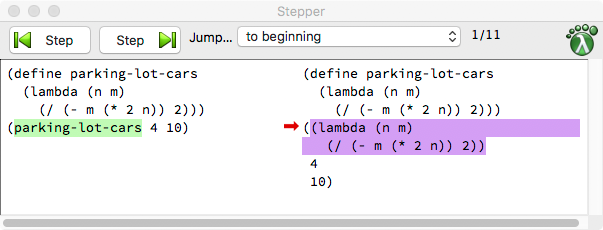
\includegraphics[width=\textwidth]{i1prog/stepper.png}
%   \caption{Stepper in DrRacket}
%   \label{fig:stepper}
% \end{figure}
% %
% Normalerweise zeigt uns DrRacket nur das Endergebnis dieses Prozesses
% an.  Es ist aber auch in der Lage, die Schritte einzeln zu
% visualisieren: Dazu müssen Sie auf den \texttt{Step}-Knopf drücken.
% Es erscheint ein neues Fenster, der sogenannte \textit{Stepper}\index{Stepper}.
% Sie können dann vorwärts und rückwärts durch den Substitutionsprozeß
% navigieren.  Abbildung~\ref{fig:stepper} zeigt das Stepper-Fenster.

\section*{Aufgaben}



\begin{aufgabe}
 Vervielfachung von Strings:
 \begin{itemize}
  \item Schreibe eine Funktion \texttt{double-string}, die eine Zeichenkette konsumiert und
    diese "`verdoppelt"', d.h., für eine Eingabe \verb|"Sperber"| den
    Rückgabewert \verb|"SperberSperber"| liefert.
    
  \item Schreibe eine Funktion \texttt{quadruple-string}, die eine
    Zeichenkette konsumiert und "`vervierfacht"'.

  \item Schreibe eine Funktion \texttt{octuple-string}, die eine
    Zeichenkette konsumiert und "`verachtfacht"'.

  \item Schreibe eine Funktion \texttt{sixteentuple-string}, die
    eine Zeichenkette konsumiert und "`versechzehnfacht"'.
  \end{itemize}
  % Schreibe für jede Funktion Kurzbeschreibung, Signatur, Testfälle, Gerüst und Rumpf.

%Vermeide bei all diesen Aufgaben, Code mehrfach zu schreiben.

\end{aufgabe}

\begin{aufgabe}

 Ein Boot überquert einen Fluss mit Strömung und
  kommt durch die Strömung vom geplanten Kurs ab.  Dadurch wird die
  Strecke, die das Boot tatsächlich zurücklegt, länger.

  \begin{center}
    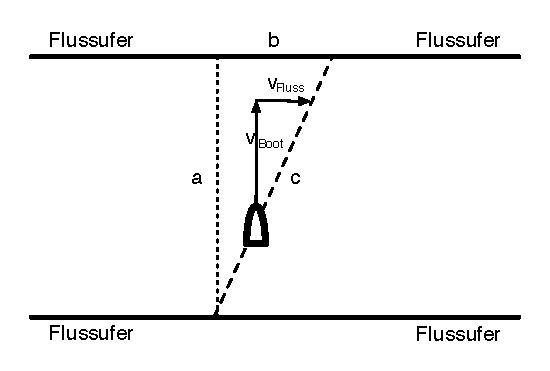
\includegraphics{riverboat}
  \end{center}

  Gegeben ist die Breite des Flusses $a$, die Strömungsgeschwindigkeit
  des Flusses $v_{\text{Fluss}}$ und die Geschwindigkeit des Bootes
  $v_{\text{Boot}}$.  Berechne die Länge der Strecke, die das
  Boot tatsächlich zurücklegt.  Programmiere dazu Funktionen, die
  folgende Teilprobleme lösen:

  \begin{enumerate}
  \item Schreibe zunächst eine Funktion \texttt{speed-ratio}, die
    das Verhältnis der Strömungsgeschwindigkeit des Flusses
    $v_{\text{Fluss}}$ zur Geschwindigkeit des Bootes
    $v_{\text{Boot}}$ berechnet.

  \item Schreibe dann eine Funktion \texttt{other-shore-offset},
    die die Länge der Strecke berechnet, die das Boot abgetrieben wird
    (also den Versatz am anderen Ufer, im Schaubild die Strecke $b$).
    % Dazu musst Du die Breite des Flusses $a$ mit dem Verhältnis von
    % $v_{\text{Fluss}}$ zu $v_{\text{Boot}}$ multiplizieren.

  \item Um $c$ zu berechnen, brauchst Du den \textit{Satz des
      Pythagoras}:
    \begin{displaymath}
      a^2 + b^2 = c^2
    \end{displaymath}
    Schreibe eine Funktion \texttt{pythagoras}, die $c$ der
    obigen Gleichung berechnet.  Erkenne und abstrahiere weitere
    Teilprobleme!

  \item Schreibe schließlich eine Funktion
    \texttt{boat-travel-distance}, die die tatsächliche Strecke
    berechnet, die das Boot zurücklegt.  Benutze dafür die bisher
    geschriebenen Funktionen.
  \end{enumerate}
\end{aufgabe}

\begin{aufgabe}

  In den USA und in Europa gibt es unterschiedliche
  Maße für die Energieeffizienz von Kraftfahrzeugen:
  \begin{itemize}
  \item In Europa ist das gängige Maß der \emph{Verbrauch} in Liter
    pro 100km (l/100km);
  \item in den USA ist das gängige Maß die \emph{Reichweite} in Meilen
    pro Gallone (mi/gal).
  \end{itemize}
  Schreibe Funktionen, die zwischen beiden Maßeinheiten
  umrechnen.  Gehe dazu wie folgt vor:

  Halte sich bei jeder Funktion, die Du schreibst, an den
  Ablauf: Schreibe zuerst die Kurzbeschreibung
  und die Signatur.  Schreibe als nächstes einige Testfälle.
  Leite Sie danach das Gerüst von der Signatur her und vervollständige
  den Rumpf der Funktion.

  \begin{enumerate}

  \item Schreibe eine Funktion
    \texttt{liters-per-hundred-kilometers}, die eine Menge Benzin in
    Liter und die Reichweite dieses Benzins in Kilometer akzeptiert
    und daraus den Verbrauch in Liter pro 100km berechnet.

  \item Schreibe eine Funktion
    \texttt{miles-per-gallon}, die eine Entfernung in Meilen und den
    Benzinverbrauch auf diese Entfernung in Gallonen akzeptiert und
    daraus die Reichweite in Meilen pro Gallone berechnet.

  \item Definiere eine Konstante
    \texttt{kilometers-per-mile} (eine US-Meile entspricht etwa $1,61$
    Kilometer) und schreibe zwei Funktionen
    \texttt{kilometers->miles} und \texttt{miles->kilometers}, die
    jeweils eine Entfernung in einer Maßeinheit akzeptieren und die
    Entfernung in die jeweils andere Maßeinheit umrechnen.

  \item Definiere eine Konstante
    \texttt{liters-per-gallon} (eine Gallone entspricht etwa $3,79$
    Liter) und schreibe zwei Funktionen \texttt{liters->gallons}
    und \texttt{gallons->liters}, die jeweils eine Menge in einer
    Maßeinheit akzeptieren und die Menge in die jeweils andere
    Maßeinheit umrechnen.

  \item Schreibe die Funktion
    \texttt{l/100km->mi/gal}, die einen Verbrauch in Liter pro 100km
    akzeptiert und in die Reichweite in Meilen pro Gallone umrechnet.
    Benutze dafür die Funktionen, die Du in den anderen
    Teilaufgaben erstellt hast.  Solltest Du auf weitere Teilprobleme
    stoßen, abstrahiere diese Teilprobleme in eigene Funktionen.

  \item Schreibe die Funktion
    \texttt{mi/gal->l/100km}, die eine Reichweite in Meilen pro
    Gallone akzeptiert und in den Verbrauch in Liter pro 100km
    umrechnet.  Benutze dafür die Funktionen, die Du in den
    anderen Teilaufgaben erstellt hast.  Solltest Du auf weitere
    Teilprobleme stoßen, abstrahiere diese Teilprobleme in eigene
    Funktionen.

  \item Finde heraus, wie hoch der Benzinverbrauch
    verschiedener Kraftfahrzeuge ist, die Du täglich im
    Straßenverkehr in Deutschland siehst.  Vergleiche diesen
    Verbrauch mit den Reichweitenangaben typischer Kraftfahrzeuge für
    den US-amerikanischen Markt.
  \end{enumerate}

\end{aufgabe}

% In vielen Ländern sind die Benzinpreise ein Grund zur allgemeinen
% Aufregung. In Deutschland wird immer die magische Marke von 1,50
% Euro pro Liter genannt, die USA haben große Angst vor der 4 Dollar
% pro Gallone. Auch sind Spritsparende Autos immer beliebter, in
% Deutschland wird auf das 3 Liter auf 100km Auto gehofft, die USA
% wünschen sich mehr 55 Meilen pro Gallone Autos.  Diese verschiedenen
% Maßstäbe sind verwirrend.

% FIXME: Hier taucht noch "Substitutionsmodell" auf.

% FIXME: umbenennen von n und m in parking-lot-cars in sprechende Namen

%%% Local Variables: 
%%% mode: latex
%%% TeX-master: "i1"
%%% End: 


% Diese Datei ist Teil des Buchs "Schreibe Dein Programm!"
% Das Buch ist lizensiert unter der Creative-Commons-Lizenz
% "Namensnennung 4.0 International (CC BY 4.0)"
% http://creativecommons.org/licenses/by/4.0/deed.de

\chapter{Fallunterscheidungen und Verzweigungen}
\label{cha:conditionals}

Computerprogramme müssen bei manchen Daten, die sie
verarbeiten, zwischen verschiedenen Möglichkeiten differenzieren: Ist
die Wassertemperatur warm genug zum Baden?  Welche von fünf
Tupperschüsseln ist für eine bestimmte Menge Kartoffelsalat groß
genug?  Welches ist die richtige Abzweigung nach Dortmund?  Solche
Entscheidungen sind daran festgemacht, dass ein Wert zu einer von mehreren
verschiedenen 
Kategorien gehören kann~-- es handelt sich dann um eine sogenannte
\textit{Fallunterscheidung\index{Fallunterscheidung}}; 
mathematische Funktionen und Programm-Funktionen operieren auf Daten mit
Fallunterscheidung durch \textit{Verzweigungen\index{Verzweigung}}.
Um diese geht es in diesem Kapitel.

\section{Rechnen mit booleschen Werten}

Für die Programme dieses Kapitels benötigen wir eine neue Art von
Daten.  Die ergeben sich, wenn wir zum Beispiel zwei Zahlen
vergleichen:
%
\begin{alltt}
(< 0 5)
\evalsto{} #t
\end{alltt}
%
\texttt{(< 0 5)} ist die Schreibweise für $0 < 5$.  Das
\verb|#t| steht für "`true\index{true}"' oder "`wahr\index{wahr}"',
denn die Aussage "`ist 0 kleiner als 5"' stimmt ja.
Umgekehrt kommt natürlich nicht \verb|#t| heraus:
%
\begin{alltt}
(< 5 0)
\evalsto{} #f
\end{alltt}
%
Das \verb|#f| steht für "`false\index{false}"' oder
"`falsch\index{falsch}"', denn diese Aussage stimmt nicht.

"`Wahr"' und "`falsch"' heißen zusammen \textit{boolesche
  Werte\index{boolescher Wert}} oder auch
\textit{Wahrheitswerte\index{Wahrheitswert}}.\footnote{Die booleschen
  Werte sind benannt nach \textit{George Boole} (1815--1864), der als
  erster einen algebraischen Ansatz für die Behandlung von Logik mit
  den Werten "`wahr"' und "`falsch"' formulierte.}  Ein Ausdruck, bei
dem ein boolescher Wert herauskommt, heißt dementsprechend auch
\textit{boolescher Ausdruck\index{boolescher Ausdruck}}.

Wir werden boolesche Ausdrücke oft
\textit{Bedingungen\index{Bedingung}} nennen.  Wenn eine Bedingung
\verb|#t| liefert, werden wir auch die Sprachregelung benutzen, dass
die Bedingung \textit{gilt}~-- beziehungsweise, dass, wenn sie
\verb|#f| liefert, sie \textit{nicht gilt}.

\texttt{<}\index{<@\texttt{<}} ist eine eingebaute Funktion, die
auf "`kleiner gleich"' testet, also dem mathematischen Operator $<$
entspricht.  Ebenso gibt es auch \texttt{>}\index{>@\texttt{>}} für
"`größer als"' (Mathematik: $>$), \texttt{=}\index{=@\texttt{=}} für
"`gleich"' (Mathematik: $=$), \texttt{<=}\index{<@\texttt{<=}} für "`kleiner oder
gleich"' (Mathematik: $\leq$) und \texttt{>=}\index{>=@\texttt{>=}}
für "`größer oder gleich"' (Mathematik: $\geq$).

Analog zu \texttt{=} für Zahlen können Zeichenketten mit
\texttt{string=?}\index{string=?@\texttt{string=?}} verglichen werden:
\begin{alltt}
(string=? "Mike" "Mike")
\evalsto{} #t
(string=? "Herbert" "Mike")
\evalsto{} #f
\end{alltt}
%
\verb|#t| und \verb|#f| sind wie Zahlen Literale, können also
auch in Programmen stehen:
%
\begin{alltt}
#t
\evalsto{} #t
#f
\evalsto{} #f
\end{alltt}
%
Programme können mit booleschen Werten auch rechnen.  Ein Ausdruck der
Form\index{and@\texttt{and}}
%
\begin{alltt}
(and \(e\sb{1}\) \(e\sb{2}\) \(\ldots\) \(e\sb{n}\))
\end{alltt}
%
ergibt immer dann \verb|#t|, wenn alle $e_i$ \verb|#t| ergeben, sonst
\verb|#f|.  Bei zwei Operanden $e_1$ und $e_2$ ergibt \texttt{(and
  $e_1$ $e_2$)} immer dann \verb|#t|, wenn $e_1$ \emph{und} $e_2$
\verb|#t| ergeben:\ref{page:and}
%
\begin{alltt}
(and #t #t)
\evalsto{} #t
(and #f #t)
\evalsto{} #f
(and #t #f)
\evalsto{} #f
(and #f #f)
\evalsto{} #f
\end{alltt}
%
Entsprechend gibt es Ausdrücke der Form\index{or@\texttt{or}}
%
\begin{alltt}
(or \(e\sb{1}\) \(e\sb{2}\) \(\ldots\) \(e\sb{n}\))
\end{alltt}
%
die immer dann \verb|#t| ergeben, wenn \emph{einer} der $e_i$ \verb|#t| ergibt, sonst
\verb|#f|.  Bei zwei Operanden $e_1$ und $e_2$ ergibt \texttt{(or
  $e_1$ $e_2$)} immer dann \verb|#t|, wenn $e_1$ \emph{oder} $e_2$
\verb|#t| ergeben:
%
\begin{alltt}
(or #t #t)
\evalsto{} #t
(or #f #t)
\evalsto{} #t
(or #t #f)
\evalsto{} #t
(or #f #f)
\evalsto{} #f
\end{alltt}
%
Des weiteren gibt es noch eine eingebaute Funktion
\texttt{not}\index{not@\texttt{not}}, die einen booleschen Wert
umdreht, sich also folgendermaßen verhält:
%
\begin{alltt}
(not #f)
\evalsto{} #t
(not #t)
\evalsto{} #f
\end{alltt}
%

\section{Verzweigungen}

Um Fallunterscheidungen zu demonstrieren, nehmen wir uns folgende
Beispielaufgabe vor: Wir schreiben eine Funktion, die eine Zahl (auf
Englisch) "`aufsagen"' soll.  Sie soll sich so verhalten:
%
\begin{alltt}
(say-number 0)
\evalsto{} "zero"
(say-number 0)
\evalsto{} "one"
\end{alltt}
%
Der Einfachheit halber beschränken wir uns vorläufig auf die Zahlen
von Null bis Drei.  Die Funktion hat folgende Kurzbeschreibung:
%
\begin{alltt}
; Zahl zu Text machen
\end{alltt}
%
Die Funktion macht aus einer natürlichen Zahl eine Zeichenkette und
hat folgende Signatur:\index{say-number@\texttt{say-number}}
%
\begin{alltt}
(: say-number (natural -> string))
\end{alltt}
%
Die Signatur sagt leider nichts darüber aus, dass die Funktion nur bis
Drei funktioniert~-- später werden wir noch beschreiben, wie die
Signatur präziser werden kann.  Hier wollten wir uns jedoch erst
einmal auf die Funktionsdefinition konzentrieren.  Vorher machen wir
aber die obigen Beispiele zu Testfällen und fügen noch zwei hinzu:
%
\begin{alltt}
(check-expect (say-number 0) "zero")
(check-expect (say-number 1) "one")
(check-expect (say-number 2) "two")
(check-expect (say-number 3) "three")
\end{alltt}
%
Das Gerüst ergibt sich direkt aus der Signatur:
%
\begin{alltt}
(define say-number
  (lambda (n)
    \ldots))
\end{alltt}
%
Aber wie kommen wir jetzt weiter?  Die Eingabe zerfällt ja in vier
Fälle~-- 0, 1, 2 und 3~-- sie bildet somit eine
\textit{Fallunterscheidung\index{Fallunterscheidung}}.  Um eine
Fallunterscheidung in der Eingabe einer Funktion verarbeiten zu können,
benötigen wir ein neues Programmelement, die
\textit{Verzeweigung\index{Verzweigung}}.  Verzweigungen beginnen mit
dem Wort \texttt{cond} und gehören zu den kompliziertesten
Programmelementen, die wir in diesem Buch benutzen.  Aber keine Sorge,
so schlimm wird es nicht.  Um eine Verzweigung zu schreiben, müssen
wir wissen, \emph{wie viele} Fälle es gibt.  In diesem Fall sind das
vier.  Die Verzewigung dafür hat folgende Form:
%

\begin{alltt}
(define say-number
  (lambda (n)
    (cond
      (\ldots{} \ldots)
      (\ldots{} \ldots)
      (\ldots{} \ldots)
      (\ldots{} \ldots))))
\end{alltt}
%
Jeder von den beiden \texttt{(\ldots \ldots)} ist ein sogenannter
\textit{Zweig\index{Zweig}}.  Der erste Teil eines Zweigs ist immer
eine Bedingung, der für den entsprechenden Fall \verb|#t| liefern
sollte und für die anderen Fälle \verb|#f|.  In diesem Fall muss die
Bedingung jedes Zweiges jeweils eine der Zahlen von Null bis Drei
identifizieren:
%
\begin{alltt}
(define say-number
  (lambda (n)
    (cond
      ((= n 0) \ldots")
      ((= n 1) \ldots)
      ((= n 2) \ldots)
      ((= n 3) \ldots))))
\end{alltt}
%
Der jeweils zweite Teil des Zweiges ist das gewünschte Ergebnis für
den entsprechenden Fall.  Wenn wir das ausfüllen, sieht das Resultat
so aus:
%
\begin{alltt}
(define say-number
  (lambda (n)
    (cond
      ((= n 0) "zero")
      ((= n 1) "one")
      ((= n 2) "two")
      ((= n 3) "three"))))
\end{alltt}
%
Fertig!
\begin{aufgabe}
  Finde heraus was passiert, wenn Du die Funktion mit einer Zahl
  aufrufst, für die sie nicht gemacht ist.
\end{aufgabe}

\section{Aufzählungen}

Nächste Beispielaufgabe: Wir wollen Haustiere einteilen in niedliche
und nicht so niedliche.  Es gibt in der Welt dieser Aufgabe nur drei
verschiedene Haustiere: Katzen, Hunde und Pythons.  Die Haustiere
bilden eine sogenannte \textit{Aufzählung\index{Aufzählung}}, die wir
in einem Kommentar im Programm so beschreiben könnten:
%
\label{sec:datendefinition}
\begin{verbatim}
; Ein Haustier ist eins der folgenden:
; - Katze
; - Hund
; - Schlange
\end{verbatim}
%
Solch ein kurzen Kommentar, der die Daten beschreibt, die in unserer
Aufgabe vorkommen, heißt
\textit{Datendefinition\index{Datendefinition}}.  Mehr dazu in Abschnitt~\ref{sec:datenanalyse}

Dass es sich um eine Aufzählung handelt, erkennen wir an der
Datendefinition: Wir benötigen für unsere Aufgabe nur die Information,
um welche Alternative aus der Datendefinition es geht~-- hier: welches
Haustier.  Für die Elemente einer Aufzählung benutzen wir 
Zeichenketten mit dem entsprechenden Text, also \verb|"Katze"|,
\verb|"Hund"| und \verb|"Schlange"|.

Für die Aufzählung der Haustiere gibt es noch keine fertige Signatur,
die müssen wir deshalb erst noch definieren.  Die
\textit{Signatur-Definition\index{Signatur-Definition}} sieht so aus:
%
\begin{alltt}
(define pet
  (signature (one-of "Katze" "Hund" "Schlange")))
\end{alltt}
%
Da sind gleich zwei neue Programmelemente drin:
%
\begin{itemize}
\item \texttt{Signature\index{signature@\texttt{signature}}} müssen wir immer schreiben, wenn wir eine
  neue Signatur erzeugen.
\item \texttt{One-of\index{one-of@\texttt{one-of}}} (das funktioniert
  nur innerhalb eines \texttt{signature}-Ausdrucks) ist für
  Aufzählungen zuständig.  In einem \texttt{one-of}-Ausdruck stehen
  die Werte, die zur Aufzählung gehören.
\end{itemize}
%
\begin{aufgabe}
  Die Funktion \texttt{say-number} aus dem vorigen Abschnitt hat ja als
  Signatur-Deklaration die folgende:
\begin{alltt}
(: say-number (natural -> string))
\end{alltt}
  % 
  Mach die Signatur präziser mit Hilfe von Datendefinitionen und
  Signatur-Definitionen!
\end{aufgabe}
%
Zurück zu unserer Funktion zur Niedlichkeitsanalyse.  Die definierte
Signatur \texttt{pet} können wir nun in der Signatur-Deklaration
unserer Funktion benutzen.  Zusammen mit der Kurzbeschreibung sieht
das so aus:
%
\begin{alltt}
; Ist Haustier niedlich?
(: cute? (pet -> boolean))
\end{alltt}
%
Das Fragezeichen gehört zum Namen der Funktion und ist eine
Konvention, die wir für die Namen von Funktionen verwenden, die einen
booleschen Wert zurückgeben~-- also solche Funktionen, die eine
Ja-/Nein-Frage beantworten.

Da es nur drei Möglichkeiten für die Eingabe gibt, können wir für alle
drei jeweils einen Test schreiben:
%
\begin{alltt}
(check-expect (cute? "Katze") #t)
(check-expect (cute? "Hund") #t)
(check-expect (cute? "Schlange") #f)
\end{alltt}
%
Kommen wir zur Funktion selbst.  Zunächst einmal das Gerüst:
%
\begin{alltt}
(define cute?
  (lambda (p)
    \ldots))
\end{alltt}
%
Da es sich bei der Eingabe um eine Aufzählung, also eine
Fallunterscheidung handel, brauchen wir eine Verzweigung im Rumpf.  Da
es drei Fälle in der Aufzählung gibt, braucht die Verzweigung
ebenfalls drei Zweige:
%
\begin{alltt}
(define cute?
  (lambda (p)
    (cond
      (\ldots{} \ldots)
      (\ldots{} \ldots)
      (\ldots{} \ldots))))
\end{alltt}
%
Als nächstes müssen wir die Bedingungen schreiben, und die sollten
\texttt{p} jeweils mit \verb|"Katze"|, \verb|"Hund"| und
\verb|"Schlange"| vergleichen.  Dabei könnte man leicht auf die Idee
kommen, \verb|(= p "Katze")| etc.\ zu schreiben.  Dann kommt
allerdings eine Fehlermeldung etwa so:
%
\begin{verbatim}
=: Zahl als erstes Argument erwartet, "Katze" bekommen
\end{verbatim}
%
Die Funktion \texttt{=} fühlt sich also nur für Zahlen zuständig, für
Zeichenketten müssen wir die Funktion
\texttt{string=?\index{string=?@\texttt{string=?}}} verwenden:
%
\begin{alltt}
(define cute?
  (lambda (p)
    (cond
      ((string=? p "Katze") \ldots)
      ((string=? p "Hund") \ldots)
      ((string=? p "Schlange") \ldots))))
\end{alltt}
%
Bisher ergibt sich alles rein aus der Definition von \texttt{pet}.
Schließlich müssen wir noch die Antworten ergänzen.  Katze und Hunde
sind niedlich, Schlangen nicht:
%
\begin{alltt}
(define cute?
  (lambda (p)
    (cond
      ((string=? p "Katze") #t)
      ((string=? p "Hund") #t)
      ((string=? p "Schlange") #f))))
\end{alltt}
%
Fertig!

\section{Zahlenbereiche}
\label{sec:zahlenbereiche}

Eine weitere häufig vorkommende Art der Fallunterscheidung gibt es bei
Zahlenbereichen.

Um das zu demonstrieren, nehmen wir uns folgende Aufgabe vor: Wir
schreiben eine Funktion, die "`Wasser erhitzt"', das heißt aus einer
Wasser-Anfangstemperatur und der Temperatur, die wir an Hitze hinzufügen, die
resultierende Temperatur bestimmt.  Wir schreiben dazu drei Versionen der
Funktion:
%
\begin{itemize}
\item Die erste, naive Version addiert einfach auf die
  Anfangstemperatur die hinzugefügte Hitze.
\item Die zweite Version berücksichtigt, dass Wasser bei 100°C siedet
  und nicht heißer werden kann.
\item Die dritte Version berücksichtigt zusätzlich, dass gefrorenem
  Wasser von 0°C eine Hitze von 80°C hinzugefügt werden muss, damit es
  schmilzt und dann immer noch erst bei 0°C ist.
\end{itemize}
%
(Physikalisch ist das natürlich Umfug, aber es geht
um ein möglichst einfaches Programmier-Beispiel.)

\paragraph{Naive Version} Wir fangen mit der naiven Version an und gehen nach dem Ablauf der
Konstruktionsanleitungen vor.  Zuerst kommt also eine
Kurzbeschreibung:
%
\begin{alltt}
; Wassertemperatur nach Erhitzen berechnen, naiv
\end{alltt}
%
Als nächstes kommt die Signatur-Deklaration.  Die Anfangstemperatur
und die hinzugefügte Hitze sind die Eingaben; sie stellen wir als
reelle Zahlen dar.  Heraus kommt die Endtemperatur, auch eine reele
Zahl.  Da wir schon wissen, dass diese Version etwas einfach ist,
hängen wir eine \texttt{-0} an den Namen:
%
\begin{alltt}
(: heat-water-0 (real real -> real))
\end{alltt}                
%
Nun schreiben wir einige einfache Beispiele als Testfälle hin:
%
\begin{alltt}
(check-expect (heat-water-0 -10 20) 10)
(check-expect (heat-water-0 10 20) 30)
(check-expect (heat-water-0 90 20) 110)
\end{alltt}
%
Als nächstes kommt das Gerüst an die Reihe:
%
\begin{alltt}
(define heat-water-0
  (lambda (temp heat)
    \ldots))
\end{alltt}
%
Der Rumpf ist jetzt kein Hexenwerk, die beiden Eingaben werden
einfach addiert:
%
\begin{alltt}
(define heat-water-0
  (lambda (temp heat)
    (+ temp heat)))
\end{alltt}
%
Noch die Tests laufen lassen und fertig!

\paragraph{Siedendes Wasser} Als nächstes wollten wir berücksichtigen,
dass Wasser nicht über 100°C heiß werden kann.  Die Kurzbeschreibung
passen wir nur leicht an; die Signatur bleibt ebenfalls fast
unverändert~-- wir ändern nur den Namen und machen aus der 0 eine 1:
%
\begin{alltt}
; Wassertemperatur nach Erhitzen berechnen, Sieden berücksichtigen
(: heat-water-1 (real real -> real))
\end{alltt}
%
Bei den Tests können wir natürlich die Tests von \texttt{heat-water-0}
kopieren, aber den letzten müssen wir anpassen:
%
\begin{alltt}
(check-expect (heat-water-1 -10 20) 10)
(check-expect (heat-water-1 10 20) 30)
(check-expect (heat-water-1 90 20) 100)
\end{alltt}
%
Beim Testen ist es immer sinnvoll, auch Grenzfälle zu testen~--
schaltet die Funktion wirklich "`rum"', wenn die 100 erreicht sind.
Dazu dienen folgende zwei Testfälle:
%
\begin{alltt}
(check-expect (heat-water-1 99 1) 100)
(check-expect (heat-water-1 99 2) 100)
\end{alltt}
%
Da die Signatur die gleiche ist, ist auch das Gerüst identisch:
%
\begin{alltt}
(define heat-water-1
  (lambda (temp heat)
    \ldots))
\end{alltt}
%
Ab 100°C muss die Funktion ihr Ergebnis also anders berechnen.  Oder,
anders gesagt, die Eingaben fallen in zwei verschiedene Klassen: die,
bei denen die Summe unter 100 liegt und die, bei denen sie darüber
liegt.
Wir benötigen also ein \texttt{cond} mit zwei
Zweigen:
%
\begin{alltt}
(define heat-water-1
  (lambda (temp heat)
    (cond
      (\ldots \ldots)
      (\ldots \ldots))))
\end{alltt}
%
Wir brauchen nun eine Bedingung, die feststellt, ob die Summe aus
\texttt{temp} und \texttt{heat} unterhalb von 100 liegt (genauer:
kleiner \emph{oder gleich}, weil 100 gerade so erreichbar ist) und
eine dafür, dass die Summe darüber liegt.  Die könnten so aussehen:
%
\begin{alltt}
(<= (+ temp heat) 100)
(> (+ temp heat) 100)
\end{alltt}
%
Wenn wir diese beiden Bedingungen an die entsprechenden Stellen im
Rumpf setzen, sieht das so aus:
%
\begin{alltt}
(define heat-water-1
  (lambda (temp heat)
    (cond
      ((<= (+ temp heat) 100) \ldots)
      ((> (+ temp heat) 100) \ldots))))
\end{alltt}
%
An die Stellen nach den Bedingungen müssen wir Ausdrücke setzen, die
das Ergebnis liefern, das im jeweiligen Fall richtig ist.  Das wäre dann:
%
\begin{alltt}
(define heat-water-1
  (lambda (temp heat)
    (cond
      ((<= (+ temp heat) 100) (+ temp heat))
      ((> (+ temp heat) 100) 100))))
\end{alltt}
%
Fertig!
%
%

%
\begin{aufgabe}
  Müssen es bei den beiden Bedingungen unbedingt \verb|<=| und
  \verb|>| sein?  Was passiert, wenn Du \verb|<=| durch \verb|<|
  ersetzt und das Programm dann laufen lässt?  Was passiert, wenn Du
  dann auch das \verb|>| ersetzt~-- durch \verb|>=|?  Warum
  funktioniert das Programm dann immer noch?
\end{aufgabe}
%
\paragraph{Siendendes Wasser und Eis} Kommen wir zur "`Vollversion"'.
Zur Erinnerung: Da müssen wir noch berücksichtigen, dass gefrorenem
Wasser von 0°C eine Hitze von 80°C hinzugefügt werden muss, damit es
schmilzt und dann immer noch hat 0°C.  

Wir fangen wieder mit der Kurzbeschreibung an:
%
\begin{verbatim}
; Wassertemperatur nach Erhitzen berechnen, mit Eis & Sieden
\end{verbatim}
%
Da diese Version die letzte ist, hat sie keine Nummer mehr.  Ansonsten
ist die Signatur unverändert:
%
\begin{verbatim}
(: heat-water (real real -> real))
\end{verbatim}
%
Die Tests können wir nicht unverändert übernehmen.  Gleich der erste
funktioniert nicht mehr:
%
\begin{verbatim}
(check-expect (heat-water -10 20) 10)
\end{verbatim}
%
Das Aufwärmen des Wassers von -10°C auf 0°C erfordert nur 10°C
Wärmezufuhr, dann aber müssen erst einmal 80° weitere Wärme zugeführt
werden, damit es weiter geht.  Den Testfall müssen wir also ändern:
%
\begin{verbatim}
(check-expect (heat-water -10 20) 0)
\end{verbatim}
%
Die anderen Testfälle \texttt{heat-water-1} können so bleiben:
%
\begin{verbatim}
(check-expect (heat-water 10 20) 30)
(check-expect (heat-water 90 20) 100)
(check-expect (heat-water 99 1) 100)
(check-expect (heat-water 99 2) 100)
\end{verbatim}
%
Ein paar weitere Tests sollten aber noch genau klären, was um den
Nullpunkt herum so passiert und wo genau er überschritten wird:
%
\begin{verbatim}
(check-expect (heat-water -10 5) -5)
(check-expect (heat-water -5 60) 0)
(check-expect (heat-water -5 90) 5)
(check-expect (heat-water -1 81) 0)
(check-expect (heat-water -1 82) 1)
\end{verbatim}
%
Wieder sollten wir darüber nachdenken, in was für Fälle unsere
Eingaben zerfallen.  Da gibt es drei naheliegende Fälle:
%
\begin{enumerate}
\item Die Anfangstemperatur ist unter 0°C, es wird also Eis erwärmt.
\item Die Erwärmung würde die Wassertemperatur auf über 100°C erhöhen.
\item Alles andere~-- das Wasser fängt flüssig an und bleibt durch die
  Erwärmung flüssig.
\end{enumerate}
%
Der erste Fall hat außerdem noch drei "`Unterfälle"':
%
\begin{itemize}
\item Die Erwärmumg bleibt unter 0°C.
\item Die Erwärmung bleibt bei  0°C "`stecken"'
\item Die Erwärmung erhöht die Temperatur über den Nullpunkt hinaus.
\end{itemize}
%
So komplizierte Fallunterscheidungen sind relativ selten. Wenn sie
doch einmal auftauchen, ist besondere Sorgfalt gefragt: Darum
exerzieren wir das hier als Beispiel durch.

Fangen wir wieder mit dem Gerüst für die Funktion an:
%
\begin{alltt}
(define heat-water
  (lambda (temp heat)
    \ldots))
\end{alltt}
%
Wir wissen schon aus der Analyse der Fälle, dass es drei Fälle gibt.
Deshalb brauchen wir auch wieder ein \texttt{cond} mit drei Zweigen.
%
\begin{alltt}
(define heat-water
  (lambda (temp heat)
    (cond
      (\ldots{} \ldots)
      (\ldots{} \ldots)
      (\ldots{} \ldots))))
\end{alltt}
%
Jetzt ergänzen wir Bedingungen, die den drei Fällen entsprechen.  Um
in diesem komplizierten Fall Leserinnen zu erleichtern, die
Bedingungen den Fällen zuzuordnen, stehen diese jeweils als Kommentar darüber:
%
\begin{alltt}
(define heat-water
  (lambda (temp heat)
    (cond
      ; Die Anfangstemperatur ist unter 0°C, es wird also Eis erwärmt.
      ((< temp 0) \ldots)
      ; Die Erwärmung würde die Wassertemperatur auf über 100°C erhöhen.
      ((>= (+ temp heat) 100) \ldots)
      ; Das Wasser fängt flüssig an und bleibt durch die Erwärmung flüssig.
      ((and (>= temp 0) (< (+ temp heat) 100)) \ldots))))
\end{alltt}
%
Jetzt können wir uns daran machen, die Zweige auszufüllen.  Da der
erste Zweig (das Eis) komplizierter ist, schieben wir den erstmal vor
uns her, denn beim zweiten Zweig kommt einfach 100°C raus.  Ebenso
einfach ist der dritte Zweig, bei dem das Wasser flüssig bleibt~-- die
Antwort ist dort \texttt{(+ temp heat)}.  Der Zwischenstand sieht so
aus:
%
\begin{alltt}
(define heat-water
  (lambda (temp heat)
    (cond
      ; Die Anfangstemperatur ist unter 0°C, es wird also Eis erwärmt.
      ((< temp 0) \ldots)
      ; Die Erwärmung würde die Wassertemperatur auf über 100°C erhöhen.
      ((>= (+ temp heat) 100) 100)
      ; Das Wasser fängt flüssig an und bleibt durch die Erwärmung flüssig.
      ((and (>= temp 0) (< (+ temp heat) 100))
       (+ temp heat)))))
\end{alltt}
%
Dass wir die leichten Fälle zuerst bearbeitet haben, mag wie Faulheit
aussehen.  Ist es auch~-- aber es ist auch sinnvolle Strategie.  Sie
könnte so beschrieben werden:
%
\begin{center}
  \emph{Schreibe auf, was Du weißt.}
\end{center}
%
Auch über den ersten Zweig wissen wir etwas, nämlich dass er selbst
eine Fallunterscheidung ist mit drei Fällen.  Wir können also das
\texttt{cond} (wieder einmal) schon hinschreiben:
%
\begin{alltt}
(define heat-water
  (lambda (temp heat)
    (cond
      ; Die Anfangstemperatur ist unter 0°C, es wird also Eis erwärmt.
      ((< temp 0)
       (cond
         (\ldots{} \ldots)
         (\ldots{} \ldots)
         (\ldots{} \ldots)))
      ; Die Erwärmung würde die Wassertemperatur auf über 100°C erhöhen.
      ((>= (+ temp heat) 100) 100)
      ; Das Wasser fängt flüssig an und bleibt durch die Erwärmung flüssig.
      ((and (>= temp 0) (< (+ temp heat) 100))
       (+ temp heat)))))
\end{alltt}
%
Auch hier ist es sinnvoll, die Beschreibungen der Fälle über die
Zweige zu schreiben.  Danach ergänzen wir die Bedingungen mit
folgendem Ergebnis:
%
\begin{alltt}
(define heat-water
  (lambda (temp heat)
    (cond
      ; Die Anfangstemperatur ist unter 0°C, es wird also Eis erwärmt.
      ((< temp 0)
       (cond
         ; Die Erwärmumg bleibt unter 0°C.
         ((< (+ temp heat) 0) \ldots)
         ; Die Erwärmung bleibt bei  0°C "stecken"
         ((and (>= (+ temp heat) 0)
               (< (+ temp heat) 80))
          \ldots)
         ; Die Erwärmung erhöht die Temperatur über den Nullpunkt hinaus.
         ((and (>= (+ temp heat) 0)
               (>= (+ temp heat) 80))
          \ldots)))
      ; Die Erwärmung würde die Wassertemperatur auf über 100°C erhöhen.
      ((>= (+ temp heat) 100) 100)
      ; Das Wasser fängt flüssig an und bleibt durch die Erwärmung flüssig.
      ((and (>= temp 0) (< (+ temp heat) 100))
       (+ temp heat)))))
\end{alltt}
%
Die Bedingungen sind jetzt noch komplizierter, aber erschließen sich
hoffentlich durch genauere Betrachtungen:
%
\begin{itemize}
\item "`Die Erwärmumg bleibt unter 0°C."'\\
  Das heißt, die Summe von
  Anfangstemperatur und Erwärmung ist kleiner als 0°C.
\item "`Die Erwärmung bleibt bei  0°C stecken."'\\
  Das heißt, die Summe von Temperatur und Erwärmung muss zwischen 0°C
  und 80°C liegen.
\item "`Die Erwärmung erhöht die Temperatur über den Nullpunkt hinaus."'\\
  Das Summe von Temperatur und Erwärmung geht nicht nur über 0°C
  sondern auch über 80°C hinaus.
\end{itemize}
%
Die Antworten unter diesen Bedingungen sind vergleichweise einfach zu
ergänzen:
%
\begin{alltt}
(define heat-water
  (lambda (temp heat)
    (cond
      ; Die Anfangstemperatur ist unter 0°C, es wird also Eis erwärmt.
      ((< temp 0)
       (cond
         ; Die Erwärmumg bleibt unter 0°C.
         ((< (+ temp heat) 0) (+ temp heat))
         ; Die Erwärmung bleibt bei  0°C "stecken"
         ((and (>= (+ temp heat) 0)
               (< (+ temp heat) 80))
          0)
         ; Die Erwärmung erhöht die Temperatur über den Nullpunkt hinaus.
         ((and (>= (+ temp heat) 0)
               (>= (+ temp heat) 80))
          (- (+ temp heat) 80))))
      ; Die Erwärmung würde die Wassertemperatur auf über 100°C erhöhen.
      ((>= (+ temp heat) 100) 100)
      ; Das Wasser fängt flüssig an und bleibt durch die Erwärmung flüssig.
      ((and (>= temp 0) (< (+ temp heat) 100))
       (+ temp heat)))))
\end{alltt}
%
Fertig!\footnote{Allerdings noch nicht ganz richtig: Vielleicht siehst Du,
  dass da noch etwas nicht ganz stimmt.  Wir kommen später darauf zurück.}

\medskip

Also \emph{fast} fertig.  Wenn wir das Programm näher betrachten,
fällt etwas Verbesserungspotenzial auf.  Fangen wir an mit der
Bedingung:
%
\begin{verbatim}
          (and (>= (+ temp heat) 0)
               (>= (+ temp heat) 80))
\end{verbatim}
%
Das ist übertrieben: Eine Temperatur über 80°C liegt auch über 0°C.
Wir können das also vereinfachen auf:
%
\begin{verbatim}
          (>= (+ temp heat) 80)
\end{verbatim}
%
Das ist mathematisch einleuchtend, zur Sicherheit sollten wir aber die
Tests nochmals laufen lassen: Aber sie laufen alle noch erfolgreich
durch.

Bevor wir die Funktion noch weiter vereinfachen, ist es sinnvoll, die
Funktionsweis eder Auswertung von \texttt{cond}-Ausdrücken zu ergründen:
%
\begin{aufgabe}
  Lasse die \texttt{heat-water}-Funktion im Stepper laufen und
  beobachte, wie~-- vor allem in welche Reihenfolge~-- die Bedindungen
  in einem \texttt{cond}-Ausdruck ausgewertet werden.
\end{aufgabe}
%
Wenn Du diese Aufgabe erledigt hast, wirst Du beobachtet haben, dass Racket
die Bedingungen in einem \texttt{cond}-Ausdruck nacheinander
auswertet.  Sobald eine davon \verb|#t| ergibt, macht Racket mit dem
Ausdruck des Zweiges weiter.  Die restlichen Zweige werden gar nicht
mehr berücksichtigt, unabhängig davon, ob sie \verb|#t| ergeben
könnten oder nicht.
Das können wir ausnutzen, um die Funktion weiter zu vereinfachen.
Dazu betrachten wir die beiden ersten Bedingungen im "`inneren"'
\texttt{cond}:
%
\begin{alltt}
       (cond
         ((< (+ temp heat) 0) (+ temp heat))
         ((and (>= (+ temp heat) 0)
               (< (+ temp heat) 80))
          0)
         \ldots)
\end{alltt}
%
Wenn die erste Bedingung \verb|#f| ergeben hat, also nicht stimmt,
dann ist \texttt{(+ temp heat)} größer oder gleich 0.  Das heißt, der
Teilausdruck \texttt{(>= (+ temp heat) 0)} in der \emph{nächsten}
Bedingung liefert \emph{immer} \verb|#t|.  Wir können also
vereinfachen:
%
\begin{alltt}
       (cond
         ((< (+ temp heat) 0) (+ temp heat))
         ((and #t
               (< (+ temp heat) 80))
          0)
         \ldots)
\end{alltt}
%
Ein Ausdruck \texttt{(and \#t \(e\))} liefert immer das gleiche Ergebnis
wie \(e\)~-- schau nochmal auf Seite~\pageref{page:and}, um Dich davon
zu überzeugen!  Wir können also das innere \texttt{cond} weiter
vereinfachen zu:
%
\begin{alltt}
       (cond
         ((< (+ temp heat) 0) (+ temp heat))
         ((< (+ temp heat) 80) 0)
         \ldots)
\end{alltt}
%
Wir benutzen also Mathematik (genauer gesagt
\textit{Algebra\index{Algebra}}, also die Lehre der Gleichungen), um
unser Programm zu vereinfachen.  Algebra ist ein sehr mächtiges
Werkzeug in der Programmierung, und wir werden es noch oft nutzen.
Das fällt oft einfacher, wenn wir gar nicht über die konkrete
Bedeutung der Ausdrücke nachdenken sondern nur Gleichungen benutzen,
wie oft in der Mathematik.

Wir sind aber mit dem Vereinfachen noch nicht fertig. Betrachten wir
nun die drei "`äußeren"' Bedingungen:
%
\begin{alltt}
    (cond
      ((< temp 0) \ldots)
      ((>= (+ temp heat) 100) \ldots)
      ((and (>= temp 0) (< (+ temp heat) 100)) \ldots))
\end{alltt}
%
Wenn die erste Bedingungen \verb|#f| ergibt, gilt automatisch
\texttt{(>= temp 0)}.  Wir können die letzte Bedingung also
vereinfachen zu:
%
\begin{alltt}
(and #t (< (+ temp heat) 100))
\end{alltt}
%
Wenn auch die zweite Bedingung \verb|#f| ergibt, gilt auch \texttt{(<
  (+ temp heat) 100)}.  Wir können also vereinfachen zu \texttt{(and
  \#t \#t)} und von da zu \verb|#t|.

Wir können die Funktion mit dieser Einsicht vereinfachen und \verb|#t|
als Bedingung hinschreiben.  (Probier es aus!)  Allerdings finden
manche das hässlich: Darum ist es auch möglich, statt \verb|#t| das
besondere Wort \texttt{else\index{else@\texttt{else}}}
("`andernfalls"' auf Englisch) hinzuschreiben.
Der \texttt{else}-Zweig kommt also zum Zug, wenn alle anderen
"`durchgefallen"' sind.  Das Ergebnis sieht
dann so aus:
%
\begin{verbatim}
(define heat-water
  (lambda (temp heat)
    (cond
      ; Die Anfangstemperatur ist unter 0°C, es wird also Eis erwärmt.
      ((< temp 0)
       (cond
         ; Die Erwärmumg bleibt unter 0°C.
         ((< (+ temp heat) 0) (+ temp heat))
         ; Die Erwärmung bleibt bei  0°C "stecken"
         ((< (+ temp heat) 80) 0)
         ; Die Erwärmung erhöht die Temperatur über den Nullpunkt hinaus.
         (else (- (+ temp heat) 80))))
      ; Die Erwärmung würde die Wassertemperatur auf über 100°C erhöhen.
      ((>= (+ temp heat) 100) 100)
      ; Das Wasser fängt flüssig an und bleibt durch die Erwärmung flüssig.
      (else
       (+ temp heat)))))
\end{verbatim}
%
\begin{feature}{Verzweigung}{scheme:cond}
In den Lehrsprachen werden Verzweigungen\index{Verzweigung}\index{Verzweigung}
mit der Spezialform \texttt{cond}\index{cond@\texttt{cond}} dargestellt.
Ein \texttt{cond}"=Ausdruck hat die folgende Form:
%
\begin{alltt}
(cond
  (\(b\sb{1}\) \(a\sb{1}\))
  (\(b\sb{2}\) \(a\sb{2}\))
  \(\ldots\)
  (\(b\sb{n-1}\) \(a\sb{n-1}\))
  (else \(a\sb{n}\))))
\end{alltt}
%
Dabei sind die $b_i$ und die $a_i$ ihrerseits Ausdrücke.  Der
\texttt{cond}-Ausdruck wertet nacheinander alle Bedingungen $b_i$ aus;
sobald eine Bedingung $b_k$ \texttt{\#t} ergibt, wird der
\texttt{cond}-Ausdruck durch das entsprechende $a_k$ ersetzt.  Wenn
alle Bedingungen fehlschlagen, wird durch $a_n$ ersetzt.  Die Paarungen
\texttt{($b_i$ $a_i$)} heißen \textit{Zweige\index{Zweig}} des
\texttt{cond}-Ausdruckes, und der Zweig mit \texttt{else}  heißt
\textit{\texttt{else}-Zweig\index{else-Zweig@\texttt{else}-Zweig}}.
Der \texttt{else}-Zweig kann auch fehlen~-- dann sollte aber immer
eine der Bedingungen  \texttt{\#t} ergeben.  Wenn doch einmal bei allen
$b_i$ \verb|#f| herauskommen sollte, bricht \drscheme{} das Programm ab
und gibt eine Fehlermeldung aus.
\end{feature}
%
Damit haben wir die komplette Funktionsweise von \texttt{cond}
angewendet. Abbildung~\ref{scheme:cond} fasst sie noch einmal zusammen.

Dann kannst Du auch von vornherein \texttt{else} benutzen, wenn Du Dir
sicher bist, dass alle anderen Fälle schon in den vorigen Zweigen
abgedeckt sind.  Im Zweifelsfall empfehlen wir aber immer den Weg über
die Mathematik, damit die Funktion auch korrekt wird.

A propos korrekt: Ist \texttt{heat-water} korrekt?  Hier ist ein
weiterer Testfall:
%
\begin{verbatim}
(check-expect (heat-water -1 191) 100)
\end{verbatim}
%
Von den 191°C wird 1°C benötigt, um auf 0°C zu kommen, dann weitere
80°C, um über 0°C hinauszukommen, bleiben 110°C.  Aber über 100°C geht
es natürlich trotzdem nicht.  Leider sieht die Funktion das anders:
%
\begin{verbatim}
Check-Fehler:
	Der tatsächliche Wert 110 ist nicht der erwartete Wert 100.
\end{verbatim}
%
Woran liegt das?  Wenn wir die Verzweigungen im Kopf nachvollziehen,
sehen wir, dass zunächst der erste Zweig des äußeren \texttt{cond}
greift, weil die Bedingung \verb|(< temp 0)| als Wert \verb|#t| hat.
Im inneren \texttt{cond} schließlich ergeben die ersten beiden
Bedingungen jeweils \verb|#f|, es bleibt also der \texttt{else}-Zweig,
und addiert die Wärme "`blind"' auf die Anfangstemperatur.

Wir müssen also unser Programm korrigieren, weil dieser Fall noch
nicht berücksichtigt ist: Die Anfangstemperatur ist unter 0°C, die
Erwärmung würde die Temperatur aber über 100°C heben.  Es greift also
der \texttt{else}-Zweig des inneren \texttt{cond} des äußeren Zweigs
mit \texttt{(< temp 0)}, und das ist in diesem Fall falsch.  Die
ersten beiden Zweige sind für Endtemperaturen bis 0°C zuständig, wir
müssen also den neuen Zweig unmittelbar vor dem \texttt{else}-Zweig
einfügen.  Der sieht so aus:
%
\begin{verbatim}
         ; Die Erwärmung würde die Temperatur auf über 100°C bringen
         ((>= (- (+ temp heat) 80) 100) 100)
\end{verbatim}
%
Jetzt ist das Programm endlich fertig und korrekt! Eine Lektion bleibt:
%
\begin{center}
  \emph{Bei komplizierten Fallunterscheidungen,\\ teste gründlich und
    gehe davon aus, dass Du Zweige vergessen hast.}
\end{center}

\section{Datenanalyse und Schablonen}
\label{sec:datenanalyse}

In Abschnitt~\ref{sec:datendefinition} auf
Seite~\pageref{sec:datendefinition} ist zum ersten Mal eine
\textit{Datendefinition\index{Datendefinition}} aufgetaucht:
%
\begin{verbatim}
; Ein Haustier ist eins der folgenden:
; - Katze
; - Hund
; - Schlange
\end{verbatim}
%
Diese Datendefinition ist das Ergebnis eines Nachdenkprozesses, der
sogenannten \textit{Datenanalyse\index{Datenanalyse}}.  Dieser Begriff
ist schon in Abschnitt~\ref{sec:konstruktionsanleitungen} auf
Seite~\pageref{sec:konstruktionsanleitungen} aufgetaucht, als zweiter
Schritt der Konstruktionsanleitung: Ab sofort werden wir diesen
Schritt immer durchführen, weil er zentral ist für die systematische
Konstruktion von Programmen.

Die Vorgehensweise bei einer Datenanalyse sieht im allgemeinen so aus:
%
\begin{konstruktionsanleitung}[Datenanalyse]
  Suche in der Aufgabenstellung nach problemrelevanten Größen suchen;
  Kandidaten sind immer die Substantive. Schreibe für jede dieser
  Größen eine Datendefinition, es sei denn, diese ist aus dem Kontext
  offensichtlich.
\end{konstruktionsanleitung}
%
In diesem Fall ist "`Haustier"' eine problemrelevante Größe, zu der
wir eine Datendefinition geschrieben haben.  Zum Bei der Erwärmung von
Wasser haben wir allerdings nicht extra hingeschrieben, dass die
Wassertemperatur eine reelle Zahl ist, weil dies allgemein bekannt
ist,

Für die Formulierung der Datendefinition gibt es eine Reihe von
typischen Mustern, die sich immer wiederfinden.  Eins ist bei der
Definition von "`Haustier"' ersichtlich, nämlich "`eins der
folgenden"', das darauf hinweist, dass es sich bei "`Haustier"' um
eine Aufzählung handelt.  Später werden wir noch andere Arten
von Daten beschreiben zusammen mit den dazu passenden Formulierungen
in den Datendefinitionen.

Die Datenanalyse spielt die zentrale Rolle bei der Umsetzung der
Konstruktionsanleitung und führt immer auch zu Elementen in unserem
Programm.  Bei der Funktion \texttt{cute?} haben wir zum Beispiel
aus der Datendefinition zunächst eine Signaturdefinition abgeleitet:
%
\begin{verbatim}
(define pet
  (signature (one-of "Katze" "Hund" "Schlange")))
\end{verbatim}
%
Da die Datendefinition für "`Haustier"' drei Fälle hat, muss auch die
Signaturdefinition drei Fälle haben.  Aus der Signaturdefinition
ergibt sich direkt eine Verzweigung im Rumpf, die sich nur aus der
Signatur \texttt{(pet -> boolean)} beziehungsweise der
Signaturdefinition von \texttt{pet} als Aufzählung mit drei Fällen
ergibt:
%
\begin{alltt}
(define cute?
  (lambda (p)
    (cond
      (\ldots{} \ldots)
      (\ldots{} \ldots)
      (\ldots{} \ldots))))
\end{alltt}
%
Da \texttt{cute?} eine Eingabe zur Signatur \texttt{pet} erwartet und
\texttt{pet} eine Aufzählungssignatur mit \emph{drei} Fällen ist, \emph{muss}
im Rumpf eine Verzweigung mit ihrerseits \emph{drei} Zweigen
auftauchen, ganz egal, was die konkrete Aufgabenstellung ist.  Wir
betonen das Wort \emph{drei} deshalb so, weil viele Fehler dadurch
passieren, dass die Anzahl der Zweige im \texttt{cond} einer solchen
Funktion nicht der Anzahl der Fälle entspricht.

So ein unfertiges Programm, in dem sich einige Elemente aus der
Analyse der Daten ergeben haben ohne besondere Berücksichtigung der
konkreten Aufgabenstellung heißt \textit{Schablone}.  Zu bestimmten
Arten von Datendefinitionen gehören bestimmte Schablonen.  Für jede
Sorte von Datendefinition schreiben wir eine Konstruktionsanleitung
mit Schablone:
%
\begin{konstruktionsanleitung}[Aufzählung]
  Versuche, für die Datendefinition eine Formulierung \emph{\ldots{}
    ist eins der folgenden} zu finden und schreibe dann eine
  Auflistung aller Fälle.  Falls jedes der Fälle nur aus einem
  einzelnen Wert besteht, handelt es sich um eine
  \textit{Aufzählung\index{Aufzählung}}.

  Schreibe für jede Aufzählung eine Signaturdefinition der Form:
  % 
\begin{alltt}
(define \(s\) (signature (one-of \ldots)))
\end{alltt}
  %
  Achte darauf, dass die Anzahl der Fälle der Signaturdefinition der
  Anzahl der Fälle der Datendefinition entspricht.
  
  Wenn Du eine Funktion schreibst, die eine Aufzählung als Eingabe
  verarbeitet, schreibe in den Rump eine Verzweigung mit sovielen
  Zweigen, wie es in der Aufzählung Fälle gibt, nach folgendem Muster:
  %
\begin{alltt}
(define \(f\)
  (lambda (\(a\))
    (cond
      (\ldots{} \ldots)
      \ldots
      (\ldots{} \ldots))))
\end{alltt}
  Schreibe danach Bedingungen in die Zweige, welche die einzelnen
  Fälle voneinander unterscheiden.
\end{konstruktionsanleitung}
%
Diese Konstruktionsanleitung mag Dir ziemlich bürokratisch vorkommen,
und das ist sie auch.  Es mag Dir langweilig vorkommen, sie stur zu
befolgen, und das ist bestimmt ab und zu der Fall.  Dafür nehmen die
Konstruktionsanleitungen Dir viel Denkarbeit ab, und Du kannst Dein
Gehirn dann für die Lösung der eigentlichen Problemstellung verwenden,
wenn erst einmal die Schablone steht.  Spätestens also wenn Du vor
einer vermeintlich schweren Aufgabe stehst, wende erst einmal die
Konstruktionsanleitungen an, bevor Du Dir Sorgen machst, ob am Ende
alles aufgeht.  Was am Ende übrigbleibt, ist oft erstaunlich einfach.

\section{Aufzählungen}
\label{sec:flensburg}
\label{sec:aufzaehlungen}

Zu den "`Flensburg"'-Punkten, die es bei Verstößen gegen die
Straßenverkehrsordnung gibt, hat eine Seite im Internet folgendes zu
sagen:
%%%% Das ist leider nicht mehr die gültige Version der Punkte! HK
%
\begin{center}
  \begin{tabular}{rl}
    0 bis 3 Punkte& Keine Sanktionen\\
    4 bis 8 Punkte& Bei freiwilliger Teilnahme an Aufbauseminaren: 4 Punkte Abzug\\
    8 bis 13 Punkte& Verwarnung und Hinweis auf freiwilliges Aufbauseminar\\
    9 bis 13 Punkte& Bei freiwilliger Teilnahme an Aufbauseminaren: 2 Punkte Abzug\\
    14 bis 17 Punkte& Teilnahme an Aufbauseminar wird angeordnet\\
    14 bis 17 Punkte&
                      Bei freiwilliger Teilnahme an verkehrspsychologischer Beratung: 2 Punkte Abzug\\
    Ab 18 Punkte&
                  Führerschein wird entzogen
  \end{tabular}
\end{center}
%
Wir können zu dieser Aufstellung eine Reihe von Fragestellungen
bearbeiten, zum Beispiel welche Sanktionen durch eine bestimmte
Punktezahl verpflichtend werden oder wieviele Punkte ein Autofahrer
nach einer bestimmten Maßnahme noch auf dem Konto hat.  In jedem Fall
teilt die Aufstellung mögliche Punktezahlen in bestimmte Kategorien
ein, je nach Maßnahme.  Folgende Maßnahmen gibt es:
%
\begin{itemize}
\item nichts
\item Aufbauseminar
\item verkehrspsychologische Beratung
\item Führerscheinentzug
\end{itemize}
%
Dies ist eine \textit{Aufzählung}\index{Aufzählung}.

Wir fangen mit der Fragestellung an, welche Zwangsmaßnahme für eine
bestimmte Punktezahl angeordnet wird.  Zwangsmaßnahmen gibt es nur
drei: keine, Aufbauseminar und Führerscheinentzug, da die
verkehrspsychologische Beratung rein freiwillig ist.  Entsprechend
zerfällt die Punkteskala in drei Teile: $0-13$, $14-17$ und ab $18$.
Die Punktezahl gehört also zu einer von drei
\textit{Kategorien}\index{Kategorie}.

Wenn die Menge, aus der ein Wert kommt, in eine feste
Anzahl von Kategorien aufgeteilt wird und bei einem Wert nur die
Kategorie zählt, ist diese Menge durch eine \textit{Fallunterscheidung} definiert.
Aufzählungen sind damit auch Fallunterscheidungen.

Eine Funktion, die  aus einem Punktestand die Zwangsmaßnahme ermittelt,
sieht folgendermaßen aus:
%
\begin{displaymath}
  m(p) \deq
  \begin{cases}
    \textit{nichts} & \textrm{falls $p \leq 13$}
    \\
    \textit{Aufbauseminar} & \textrm{falls $p \geq 14, p \leq 17$}
    \\
    \textit{Führerscheinentzug } & \textrm{falls $p \geq 18$}
  \end{cases}
\end{displaymath}
%
Die Notation mit der großen geschweiften Klammer heißt
\textit{Verzweigung\index{Verzweigung}} (engl.\
\textit{conditional\index{conditional}}); ein Ausdruck wie $p\leq 13$,
der wahr oder falsch sein kann,
heißt \textit{Bedingung\index{Bedingung}}.


\section{Binäre Verzweigungen und syntaktischer Zucker}
\label{sec:binaere-verzweigungen}

Bei manchen Fallunterscheidungen definiert sich die letzte Kategorie
dadurch, dass ein Wert in keine der anderen Kategorien gehört.  Dann
ist die Benutzung eines \texttt{else}-Zweigs im \texttt{cond}
sinnvoll.
FIXME: Beispiel wäre schön, dann vielleicht früher.  
Manchmal gibt es dabei nur zwei Kategorien, wie
zum Beispiel beim Absolutbetrag.  Hier die Definition dazu in mathematischer
Schreibweise:
%
\begin{displaymath}
  |x| \deq{} \left\{\begin{array}{rl}
      x & \textrm{falls } x \geq 0\\
      -x & \textrm{andernfalls}
    \end{array}
    \right.
\end{displaymath}
%
Die dazu passende Programm-Funktion unter Verwendung von \texttt{cond}
sieht so aus:\index{abs@\texttt{abs}}
%
\begin{alltt}
; Absolutbetrag einer Zahl berechnen
(: absolute (number -> number))
(define absolute
  (lambda (x)
    (cond
     ((>= x 0) x)
     (else (- x)))))
\end{alltt}
FIXME: besseres Beispiel

%
Dieser Spezialfall mit nur zwei Kategorien, genannt \textit{binäre
  Verzweigung\index{binäre Verzweigung}\index{Verzweigung!binär}} kommt in der Praxis
häufig vor.  In den Lehrsprachen gibt es dafür eine eigene Spezialform,
genannt \texttt{if\index{if@\texttt{if}}}, die hier kürzer ausfällt
als \texttt{cond}:
%
\begin{alltt}
(define absolute
  (lambda (x)
    (if (>= x 0)
        x
        (- x))))
\end{alltt}
%
Eine \texttt{if}-Form hat folgende Form:
%
\begin{alltt}
(if \(t\) \(k\) \(a\))
\end{alltt}
Dabei ist $t$ die Bedingung und $k$ und $a$ sind die
beiden Zweige: die \textit{Konsequente\index{Konsequente}} $k$ und die
\textit{Alternative\index{Alternative}} $a$.  Abhängig vom Ausgang der
Bedingung ist der Wert der Verzweigung entweder der Wert der Konsequente
oder der Wert der Alternative.

Tatsächlich ist \texttt{if} die "`primitivere"' Form als
\texttt{cond}: jede \texttt{cond}-Form kann in eine äquivalente
\texttt{if}-Form übersetzt werden, und zwar nach
folgendem Schema:
%
\begin{alltt}
(cond (\(t\sb{1}\) \(a\sb{1}\)) (\(t\sb{2}\) \(a\sb{2}\)) \(\ldots\) (\(t\sb{n-1}\) \(a\sb{n-1}\)) (else \(a\sb{n}\)))
  \(\mapsto\) (if \(t\sb{1}\) \(a\sb{1}\) (if \(t\sb{2}\) \(a\sb{2}\) \ldots (if \(t\sb{n-1}\) \(a\sb{n-1}\) \(a\sb{n}\))\ldots))
\end{alltt}
%
Die geschachtelte \texttt{if}-Form auf der rechten Seite der
Übersetzung wertet, genau wie die \texttt{cond}-Form, nacheinander
alle Bedingungen aus, bis eine \verb|#t| liefert.  Die rechte Seite des
\texttt{cond}-Zweigs ist dann gerade die Konsequente des \texttt{if}s.
Erst wenn alle Bedingungen fehlschlagen ist die Alternative des letzten
\texttt{if}-Ausdrucks dran, nämlich $a_n$ aus dem \texttt{else}-Zweig.

Da sich mit Hilfe dieser Übersetzung jede \texttt{cond}-Form durch
geschachtelte \texttt{if}-Formen ersetzen lässt, ist \texttt{cond}
streng genommen gar nicht notwendig.  \texttt{Cond} ist deswegen eine
sogenannte \textit{abgeleitete Form\index{abgeleitete
    Form}}\index{Form!abgeleitet}.  Da \texttt{cond} und andere
abgeleitete Formen trotzdem praktisch und angenehm zu verwenden sind
und damit dem Programmierer die Arbeit versüßen,
heißen abgeleitete Formen auch \textit{syntaktischer
  Zucker\index{syntaktischer Zucker}\index{Zucker, syntaktischer}}.

Um die Funktionsweise von Verzweigungen genau zu beschreiben, dient
folgende zusätzliche Regel für das Substitutionsmodell aus
Abschnitt~\ref{sec:substitution-model}:
%
\begin{description}
\item[binäre Verzweigungen] Bei der Auswertung einer Verzweigung wird
  zunächst der Wert der Bedingung festgestellt.  Ist dieser Wert \verb|#t|,
  so ist der Wert der Verzweigung der Wert der Konsequente.  Ist er
  \verb|#f|, so ist der Wert der Verzweigung der Wert der
  Alternative.  Ist der Wert der Bedingung  kein boolescher Wert ist, ist das Programm fehlerhaft.
\end{description}
%
Auch \texttt{and} und \texttt{or} sind eigentlich syntaktischer Zucker:
Es ist immer möglich, einen \texttt{and}-Ausdruck in \texttt{if}s
zu übersetzen.  Es gelten folgende Übersetzungsregeln:
%
\begin{alltt}
(and) \(\mapsto\) #t
(and \(e\sb{1}\) \(e\sb{2}\) \(\ldots\)) \(\mapsto\) (if \(e\sb{1}\) (and \(e\sb{2}\) \(\ldots\)) #f)
\end{alltt}
%
Ein \texttt{and}-Ausdruck mit mehreren Operanden wird so schrittweise
in eine Kaskade von \texttt{if}-Ausdrücken übersetzt:
%
\begin{alltt}
(and a b c)
\(\mapsto{}\) (if a (and b c) #f)
\(\mapsto{}\) (if a (if b (and c) #f) #f)
\(\mapsto{}\) (if a (if b (if c (and) #f) #f) #f)
\(\mapsto{}\) (if a (if b (if c #t #f) #f) #f)
\end{alltt}
%
Ebenso lassen sich \texttt{or}-Ausdrücke immer in
\texttt{if}-Ausdrücke übersetzen, und zwar mit folgender Übersetzung:
%
\begin{alltt}
(or) \(\mapsto\) #f
(or \(e\sb{1}\) \(e\sb{2}\) \(\ldots\)) \(\mapsto\) (if \(e\sb{1}\) #t (or \(e\sb{2}\) \(\ldots\)))
\end{alltt}
%
Beispiel:
%
\begin{alltt}
(or a b c)
\(\mapsto{}\) (if a #t (or b c))
\(\mapsto{}\) (if a #t (if b #t (or c)))
\(\mapsto{}\) (if a #t (if b #t (if c #t (or))))
\(\mapsto{}\) (if a #t (if b #t (if c #t #f)))
\end{alltt}

\section{Signaturdefinitionen}

Nehmen wir uns zu Übungszwecken noch eine weitere Aufgabe vor: Nehmen
wir an, jemand nimmt bei einem bestimmten Punktestand in Flensburg an
einer freiwilligen Maßnahme teil~-- was ist der Punktestand nach der
Maßnahme?  Die bekannten Größen sind:
%
\begin{itemize}
\item Punktestand vor der Maßnahme (natürliche Zahl)
\item freiwillige Maßnahme (siehe Abschnitt~\ref{sec:flensburg})
\end{itemize}
%
Die unbekannte Größe ist der Punktestand nach der Maßnahme.

Die Kurzbeschreibung könnte so lauten:
%
\begin{verbatim}
; Punktestand in Flensburg senken
\end{verbatim}
%
Die Signatur folgt aus der Datenanalyse:\index{improve-points@\texttt{improve-points}}
%
\begin{verbatim}
(: improve-points (natural (one-of "nichts"
                                   "Aufbauseminar"
                                   "verkehrspsychologische Beratung"
                                   "Führerscheinentzug")
                    -> natural))
\end{verbatim}
%
Der \texttt{one-of}-Teil der Signatur macht sich da ganz schön breit,
zumal er sich weitgehend deckt mit dem entsprechenden Teil der
Signatur von \texttt{points-must-do} auf
Seite~\pageref{page:points-must-do}.  Entsprechend sollten wir genauso
wie bei anderen Werten der Signatur für "`Flensburg"=Maßnahmen"' einen
Namen geben.  Das geht mit einer fast ganz normalen Definition:\index{Signaturdefinition}
%
\begin{verbatim}
(define action
  (signature
   (one-of "nichts"
           "Aufbauseminar"
           "verkehrspsychologische Beratung"
           "Führerscheinentzug")))
\end{verbatim}
%
Das Wörtchen \texttt{signature}\index{signature@texttt{signature}}\label{page:signature} ist aus technischen Gründen
nötig.\footnote{Es sorgt unter anderem dafür, dass Signaturdefinitionen
  in beliebiger Reihenfolge geschrieben werden und die Links in den
  Fehlermeldungen von DrRacket auf die richtige Stelle zeigen.}
Faustregel: Signaturen außerhalb von Formen \texttt{(: \ldots)} müssen immer in ein \texttt{(signature
  \ldots)} eingeschachtelt werden..

Mit dieser Definition gewappnet können wir die Signatur abkürzen:
%
\begin{verbatim}
(: improve-points (natural action -> natural)) 
\end{verbatim}
%
Entsprechend Mantra~\ref{mantra:coverage} versuchen wir, durch mehr
Tests als noch bei \texttt{points-must-do} bessere Abdeckung zu
erzielen:\label{page:improve-points-tests}
%
\begin{verbatim}
(check-expect (improve-points 3 "Aufbauseminar") 3)
(check-expect (improve-points 4 "nichts") 4)
(check-expect (improve-points 4 "Aufbauseminar") 0)
(check-expect (improve-points 8 "Aufbauseminar") 4)
(check-expect (improve-points 9 "Aufbauseminar") 7)
(check-expect (improve-points 13 "Aufbauseminar") 11)
(check-expect (improve-points 14 "verkehrspsychologische Beratung") 12)
(check-expect (improve-points 17 "verkehrspsychologische Beratung") 15)
(check-expect (improve-points 18 "Aufbauseminar") 18)
(check-expect (improve-points 18 "verkehrspsychologische Beratung") 18)
\end{verbatim}
%
Hier das Gerüst:
%
\begin{verbatim}
(define improve-points
  (lambda (p a)
    ...))
\end{verbatim}
%
Bei der Konstruktion der Schablone müssen wir uns entscheiden, an
welchem Parameter wir uns orientieren, \texttt{p} oder \texttt{a}.
Die Entscheidung ist willkürlich~-- wir entscheiden uns erst einmal
für \texttt{p}.  (Ausgehend von \texttt{a} kommt eine andere aber
genauso gute Lösung heraus~-- das sei Ihnen in
Aufgabe~\ref{aufgabe:improve-points-a} als Fingerübung empfohlen.)
Bei \texttt{p} gibt es in Bezug auf diese Aufgabe fünf Kategorien:
%
\begin{description}
\item[0--3 Punkte] Da bringt keine Maßnahme etwas.
\item[4--8 Punkte] Da bringt ein Aufbauseminar 4 Punkte Abzug.
\item[9--13 Punkte] Da bringt ein Aufbauseminar 2 Punkte Abzug.
\item[14--17 Punkte] Da bringt eine verkehrspsychologische Beratung 2
  Punkte Abzug.
\item[über 18 Punkte] Auch hier hilft keine Maßnahme.
\end{description}
%
Wir brauchen also ein \texttt{cond} mit fünf Zweigen:
%
\begin{verbatim}
(define improve-points
  (lambda (p a)
    (cond
      (... ...)
      (... ...)
      (... ...)
      (... ...)
      (... ...))))
\end{verbatim}
%
Jetzt müssen wir Bedingungen erfinden, die den Kategorien entsprechen:
%
\begin{verbatim}
(define improve-points
  (lambda (p a)
    (cond
      ((<= p 3) ...)
      ((and (>= p 4) (<= p 8)) ...)
      ((and (>= p 9) (<= p 13)) ...)
      ((and (>= p 14) (<= p 17)) ...)
      ((>= p 18) ...))))
\end{verbatim}
%
Wir fangen mal mit den einfachsten Fällen an~-- unten und oben in der
Punkteskala, wo sich nichts bewegt:
%
\begin{verbatim}
(define improve-points
  (lambda (p a)
    (cond
      ((<= p 3) p)
      ((and (>= p 4) (<= p 8)) ...)
      ((and (>= p 9) (<= p 13)) ...)
      ((and (>= p 14) (<= p 17)) ...)
      ((>= p 18) p))))
\end{verbatim}
%
Im zweiten Zweig~-- zwischen vier und acht Punkten~-- zählt nur ein
Aufbauseminar, alle anderen Maßnahmen bringen nichts.  Darum ist hier
eine binäre Verzweigung angemessen:
%
\begin{verbatim}
(define improve-points
  (lambda (p a)
    (cond
      ...
      ((and (>= p 4) (<= p 8))
       (if (string=? a "Aufbauseminar")
           (- p 4)
           p))
      ...)))
\end{verbatim}
%
Entsprechend funktionieren auch der dritte und der vierte Zweig:
%
\begin{verbatim}
(define improve-points
  (lambda (p a)
    (cond
      ((<= p 3) p)
      ((and (>= p 4) (<= p 8))
       (if (string=? a "Aufbauseminar")
           (- p 4)
           p))
      ((and (>= p 9) (<= p 13))
       (if (string=? a "Aufbauseminar")
           (- p 2)
           p))
      ((and (>= p 14) (<= p 17))
       (if (string=? a "verkehrspsychologische Beratung")
           (- p 2)
           p))
      ((>= p 18) p))))
\end{verbatim}
%
Fertig!  Es gibt trotzdem noch einen Wermutstropfen: Die Abdeckung ist
trotz der vielen Tests immer noch nicht vollständig~-- siehe
Aufgabe~\ref{aufgabe:improve-points-coverage}

\section{Unsinnige Daten abfangen}
\label{sec:nonsensical-data}

Noch einmal zurück zum Parkplatzproblem, das wir auf
Seite~\ref{page:parking-lot-cars} programmiert hatten.  In
Abschnitt~\ref{sec:nonsensical-data-prequel} auf
Seite~\pageref{sec:nonsensical-data-prequel} hatten wir bereits
bemerkt, dass die Funktion
\texttt{parking-lot-cars}\index{parking-lot-cars@\texttt{parking-lot-cars}}
auch für unsinnige Daten fröhlich ebenso unsinnige Ergebnisse
ermittelt.

Auf Seite~\ref{page:parking-lot-problem} wurde bereits eine Bedingung
für sinnvolle Daten formuliert: Wenn $n$ die Anzahl der Fahrzeuge und
$m$ die Anzahl der Räder ist, dann muss $m$ gerade sein sowie $2n\leq
m\leq 4n$ gelten.  Wir können das in einer binären Verzweigung zum
Ausdruck bringen:
%
\begin{verbatim}
(define parking-lot-cars
  (lambda (vehicle-count wheel-count)
    (if (and (even? wheel-count)
             (<= (* 2 vehicle-count) wheel-count)
             (<= wheel-count (* 4 vehicle-count)))
        (/ (- wheel-count (* 2 vehicle-count))
           2)
        ...)))
\end{verbatim}
%
Die eingebaute Funktion \texttt{even?} akzeptiert eine ganze Zahl und
liefert \verb|#t|, falls die Zahl gerade ist und \verb|#f|, falls sie
ungerade ist~-- solche und viele andere nützliche Funktionen finden
Du in der Dokumentation im Hilfezentrum unter "`Sprachebenen und
Material zu \textit{Schreibe Dein Programm!}"' im Abschnitt
"`Primitive Operationen"'.

Nur~-- was tun im Fehlerfall?  Dazu gibt eine eingebaute Funktion
\texttt{violation}, die eine Fehlermeldung als Zeichenkette akzeptiert
und, wenn sie aufgerufen wird, das Programm abbricht und die
Fehlermeldung ausdruckt.  \texttt{Parking-lot-cars} sieht dann
vollständig so aus:
%
\begin{verbatim}
(define parking-lot-cars
  (lambda (vehicle-count wheel-count)
    (if (and (even? wheel-count)
             (<= (* 2 vehicle-count) wheel-count)
             (<= wheel-count (* 4 vehicle-count)))
        (/ (- wheel-count (* 2 vehicle-count))
           2)
        (violation "unsinnige Daten"))))
\end{verbatim}
%
Natürlich sollten wir auch den Fehlerfall testen~-- das geht nicht mit
\texttt{check-expect}, das ja erwartet, dass ein Testausdruck einen
ordnungsgemäßen Wert liefert.  Für Fehlerfälle gibt es
\texttt{check-error}, das Testfälle erzeugt, die dann bestanden sind,
wenn die Auswertung einen Fehler liefert:
%
\begin{verbatim}
(check-error (parking-lot-cars 10 10)) ; zu wenige Räder
(check-error (parking-lot-cars 3 9))   ; ungerade Räderzahl
(check-error (parking-lot-cars 2 10))  ; zu viele Räder
\end{verbatim}

\section*{Aufgaben}

\begin{aufgabe}
  Schreibe eine Funktion \texttt{card-type}, die den Umsatz einer
  Kreditkarte konsumiert und die eine entsprechende Kategorie als
  Zeichenkette zurückgibt.  Verwende die Konstruktionsanleitungen:
  Schreibe die Kurzbeschreibung auf, führe eine
  Datenanalyse durch und schreibe die Signatur auf. Erstelle
  dann die Testfälle und das Gerüst.  Vervollständige danach den
  Rumpf der Funktion und vergewissere Dich, dass die Tests
  erfolgreich laufen. \\

  \begin{tabular}{crlcrll}
    &        & Umsatz & $<$ & $15.000$   & $\Longrightarrow$ & Weiß \\
    $15.000$  & $\leq$ & Umsatz & $<$ & $50.000 $  & $\Longrightarrow$ & Gold \\
    $50.000$  & $\leq$ & Umsatz & $\leq$ & $150.000 $ 
    & $\Longrightarrow$ & Platin \\
    $150.000$ & $<$ & Umsatz &     &            &  $\Longrightarrow$ & Schwarz \\
  \end{tabular} \\
\end{aufgabe}

\begin{aufgabe}

  \begin{enumerate}

  \item Schreibe eine Funktion \texttt{min-2}, die als Argumente zwei
    Zahlen nimmt und die kleinere der beiden Zahlen zurückgibt.  Schreibe
    außerdem eine Funktion \texttt{min-3}, die als Argumente drei
    Zahlen nimmt und die kleinste der drei Zahlen zurückgibt.  Verwende
    die Konstruktionsanleitung: Schreibe
    explizit Kurzbeschreibung und Signatur auf, erstelle dann das
    Gerüst und die Testfälle.  Vervollständige danach den Rumpf der
    Funktion und vergewissere Dich, dass die Tests erfolgreich laufen.
    
  \item Schreibe analog eine Funktion \texttt{max-2} und \texttt{max-3}.
    
  \end{enumerate}
\end{aufgabe}

\begin{aufgabe}
  Schreibe die folgenden Funktionen:
  \begin{enumerate}
  \item \texttt{min-of-two}, welche die kleinste von zwei
    gegebenen Zahlen ausgibt
  \item \texttt{min-of-three}, welche die kleinste von drei
    gegebenen Zahlen ausgibt
  \item \texttt{is-min-of-three?}, die überprüft ob die erste
    von drei gegebenen Zahlen das Minimum ist
  \item \texttt{valid-value?}, die überprüft ob die erste von
    drei gegebenen Zahlen zwischen den beiden anderen liegt; gehe
    davon aus, dass der Aufruf immer \texttt{(valid-value? value min max)}
    lautet 
  \item \texttt{clamp}, die wie folgt definiert ist:
    
    \[\text{clamp}(x,\ min,\ max)=
    \begin{cases} 
      x & min \leq x \leq max\\ 
      min & x < min \\ 
      max & x > max 
    \end{cases}
    \]
    
  \end{enumerate}
\end{aufgabe}

\begin{aufgabe}
  FIXME Spielerin
  
  Beim Fußball lässt die Rückennummer eines Spielers
  häufig Rückschlüsse auf seine Position zu. Wir machen dabei folgende
  Annahmen:
  \begin{itemize}
  \item Ein \emph{Torwart} hat die Rückennummer 1.
  \item Ein \emph{Abwehrspieler} hat die Rückennummer 2, 3, 4 oder 5.
  \item Ein \emph{Mittelfeldspieler} hat die Rückennummer 6, 7, 8 oder 10.
  \item Ein \emph{Stürmer} hat die Rückennummer 9 oder 11.
  \item Ein \emph{Ersatzspieler} hat eine Rückennummer zwischen 12 und 99.
  \item Alle anderen Rückennummern sind ungültig.
  \end{itemize}
 
  Schreibe nun eine Funktion mit folgender Signatur:
  
  {\small
\begin{verbatim}
 (: nummer->position
    (number ->
      (one-of "Torwart" "Abwehr" "Mittelfeld" "Sturm" "Ersatz" "Ungültig")))
\end{verbatim}
  }

  Die Funktion soll dabei zu einer gegebenen Rückennummer die
  zugehörige Position berechnen.

  Verwende beim Schreiben der Funktion die
  Konstruktionsanleitungen für Funktionen und für
  Fallunterscheidungen.  Teste die Funktion
  \texttt{nummer->position} mit mindestens sechs Testfällen, so dass
  alle Fälle abgedeckt sind.
\end{aufgabe}


\begin{aufgabe}
  Schreibe ein Programm, mit dem Bußgelder
  automatisch bestimmt werden.
  
  \begin{enumerate}
  \item Programmiere eine Funktion \texttt{zu-langes-parken}
    für die Bewertung von zu langem Parken auf einem kostenpflichtigen
    Parkplatz. Diese bekommt eine Zeitspanne übergeben und gibt das 
    entsprechende Verwarngeld zurück.
    
    Diese Verwarnungen sind wie folgt festgelegt:
    \begin{itemize}
    \item Überschreitung der Höchstparkdauer bis 30 Minuten: \euro{5}
    \item bis zu einer Stunde: \euro{10}
    \item bis zu zwei Stunden: \euro{15}
    \item bis zu drei Stunden: \euro{20}
    \item länger als drei Stunden:  \euro{25}
    \end{itemize}
    
  \item Das Überfahren einer roten Ampel kostet je nach
    Gefährdungslage mehr, gibt Punkte und Fahrverbote. Schreibe
    zwei Funktionen, eine für das Bußgeld \texttt{rote-ampel-bußgeld}, 
    eine für die Punkte in Flensburg \texttt{rote-ampel-punkte} 
    und eine für das Fahrverbot \texttt{rote-ampel-fahrverbot}, 
    welche ausgibt, ob ein Fahrverbot erteilt wird. Übergib
    den Funktionen, wie lange die Ampel schon rot war und ob eine
    Gefährdung oder Sachbeschädigung vorlag.
    
    Die Bußgelder sind wie folgend definiert:
    \begin{itemize}
    \item Bei Rot über die Ampel innerhalb der ersten Sekunde			
      \euro{50} und 3 Punkte.
    \item Bei Rot über die Ampel innerhalb der ersten Sekunde mit
      Gefährdung oder Sachbeschädigung \euro{125}, 4 		
      Punkte und 1 Monat Fahrverbot.
    \item Bei Rot über die Ampel nach der ersten Sekunde \euro{125},
      4 Punkte und 1 Monat Fahrverbot.
    \item Bei Rot über die Ampel nach der ersten Sekunde mit
      Gefährdung oder Sachbeschädigung \euro{200}, 4
      Punkte und 1 Monat Fahrverbot.
    \end{itemize}
    
    
  \end{enumerate}
\end{aufgabe}


%%% Local Variables: 
%%% mode: latex
%%% TeX-master: "i1"
%%% End: 


% Das Buch ist lizensiert unter der Creative-Commons-Lizenz
% "Namensnennung 4.0 International (CC BY 4.0)"
% http://creativecommons.org/licenses/by/4.0/deed.de

\chapter{Zusammengesetzte Daten}
\label{cha:zusammengesetzte-daten}

TBD

Mit anderen Worten: mehrere Dinge werden \emph{zu einem}
zusammengesetzt.  Eine andere Betrachtungsweise ist, da� ein einzelnes
Ding durch mehrere Eigenschaften charakterisiert ist.

In Scheme lassen sich solche \textit{zusammengesetzte
Daten}\index{zusammengesetzte Daten} durch
\textit{Records}\index{Record} darstellen.  Ein Record ist wie ein
Beh�lter mit mehreren F�chern, in denen die Bestandteile der Daten
untergebracht sind.

\section{Computer konfigurieren}

Viele Computerh�ndler erlauben ihren Kunden, bestimmte Komponenten
eines neues Computers selbst auszuw�hlen, zum Beispiel den Prozessor,
die Festplatte oder die Gr��e des RAM-Hauptspeichers:
%
\begin{center}
  \includegraphics[height=0.3\textheight]{computer.eps}
\end{center}
%
Eine m�gliche Beschreibung dieser Situation ist:

Ein Computer\index{Computer} \emph{besteht aus}:
%
\begin{itemize}
\item Prozessor
\item RAM
\item Festplatte
\end{itemize}
%
Nat�rlich besteht ein Computer auch noch aus anderen Teilen, die
aber (zumindest in diesem Beispiel) immer gleich sind.  In einer Bestellung mu�
der Kunde also nur diese drei Bestandteile angeben.  Wir nehmen an,
da� es beim Prozessor nur auf den Namen ("`Athlon"', "`Xeon"',
"`Cell"', \ldots) ankommt, beim RAM nur auf die Gr��e in Gigabyte, und
auch bei der Festplatte nur auf die Gr��e in Gigabyte.  Eine
vereinfachte Darstellung k�nnte so aussehen:
%
\begin{center}
  Computer:
  \begin{tabular}[c]{|r|l|}
    \hline
    \textbf{Feld} & \textbf{Komponente}\\\hline
    \hline
     Prozessor & \verb|"Cell"|\\
     \hline
     RAM & 2\\
    \hline 
    Festplatte & 250\\
    \hline
  \end{tabular}
\end{center}
%
Diese Tabelle steht demnach f�r einen Computer mit Cell-Prozessor, 2
Gigabyte RAM und einer 250-Gigabyte-Festplatte.

Die Begriffe "`Feld"'\index{Feld} und "`Komponente"'\index{Komponente}
sind dabei Termini~-- das \textit{Feld} ist die Allgemeinbezeichnung
f�r ein Bestandteil, das alle Computer haben.  Die \textit{Komponente}
ist das konkrete Bestandteil eines einzelnen Computers.

Die Darstellung f�r solche \textit{zusammengesetzte
  Daten\index{zusammengesetzte Daten}}, die aus mehreren
\textit{Komponenten\index{Komponente}} (in diesem Fall "`\texttt{Cell}"', $2$
und $250$) bestehen, hei�t \textit{Record}.  Alle
Records f�r Computer geh�ren zu einer gemeinsamen Menge, dem
\textit{Record-Typ\index{Record-Typ}} f�r Computer.  (Weiter hinten
in diesem Kapitel wird beschrieben, wie ein Programm eigene
Record-Typen definieren kann.)  Der Record-Typ f�r Computer sieht
feste \textit{Felder\index{Feld}} ("`Prozessor"', "`RAM"' und "`Festplatte"') vor,
welche die Komponenten aufnehmen.  F�r jedes Feld des Record-Typs
"`Computer"' besitzt also jeder einzelne Computer jeweils eine
Komponente, in diesem Fall eine f�r das Prozessor-, eine f�r das RAM- und eine f�r das
Festplatten-Feld.

Der Computerhersteller stellt einen echten Computer her, indem er
zun�chst den Prozessor, den RAM und die Festplatte fertigstellt und
diese dann zum Computer zusammensetzt.  Umgekehrt nehmen manche
Bastler aus dem Computer die Einzelteile wieder heraus, zum Beispiel,
um sie in einem anderen Computer zu verbauen.

In der \drscheme{}-Sprachebene \texttt{Die Macht der Abstraktion - Anf�nger} sind
Computer schon eingebaut.  Ein Computer mit Cell-Prozessor, 2
Gigabyte RAM und 250 Gigabyte Festplatte wird folgenderma�en hergestellt:
%
\begin{alltt}
(make-computer "Cell" 2 250)
\evalsto{} #<record:computer "Cell" 2 250>
\end{alltt}
%
Die Prozedur \texttt{make-computer} hat folgende Signatur:
%
\begin{alltt}
(: make-computer (string rational rational -> computer))
\end{alltt}
%
Sie macht also aus einer Zeichenkette und zwei Zahlen einen Wert der eingebauten Sorte
\texttt{computer} der Computer-Records.
Die \drscheme{}-REPL druckt Record-Werte mit der Schreibweise
\verb|#<record:... ...>| aus, damit Sorte und Komponenten sichtbar
werden.

Computer sind Werte wie andere auch und lassen sich zum Beispiel an
Variablen binden:
%
\begin{alltt}
; Cell, 4 Gbyte RAM, 1000 Gbyte Festplatte
(define gamer (make-computer "Cell" 4 1000))
gamer
\evalsto{} #<record:computer "Cell" 4 1000>
; Xeon, 2 Gbyte RAM, 500 Gbyte Festplatte
(define workstation (make-computer "Xeon" 2 500))
workstation
\evalsto{} #<record:computer "Xeon" 2 500>
\end{alltt}
%
Da die Prozedur \texttt{make-computer} einen Computer
"`konstruiert"', hei�t sie auch
\textit{Konstruktor\index{Konstruktor}}.  F�r das Zerlegen von
Computern sind die Prozeduren \texttt{computer"=processor},
\texttt{computer"=ram} und \texttt{computer-hard-drive}
zust�ndig:
%
\begin{alltt}
(computer-processor gamer)
\evalsto{} "Cell"
(computer-ram gamer)
\evalsto{} 4
(computer-hard-drive gamer)
\evalsto{} 1000
\end{alltt}
%
Diese drei Prozeduren extrahieren die Bestandteile aus einem
Computer und hei�en \textit{Selektoren\index{Selektor}}.  Sie haben
folgende Signaturen:
%
\begin{alltt}
(: computer-processor (computer -> string))
(: computer-ram (computer -> rational))
(: computer-hard-drive (computer -> rational))
\end{alltt}
%
Mit Hilfe des Konstruktors und der Selektoren kann der Programmierer
weitergehende Prozeduren definieren.  F�r den Anfang k�nnte das
eine Prozedur sein, die den Gesamtspeicher eines Computers berechnet,
also Hauptspeicher und Festplattenspeicher zusammen.
Eine solche Prozedur m��te Kurzbeschreibung und Signatur wie folgt haben:\index{total-memory@\texttt{total-memory}}
%
\begin{alltt}
; Gesamtspeicher berechnen
(: total-memory (computer -> rational))
\end{alltt}
%
Hier sind unsere Erwartungen an \texttt{total-memory}, als Testf�lle
formuliert:
%
\begin{alltt}
(check-expect (total-memory workstation) 502)
(check-expect (total-memory gamer) 1004)
\end{alltt}
% 
Das Ger�st m��te folgenderma�en sein:
%
\begin{alltt}
(define total-memory
  (lambda (c)
    ...))
\end{alltt}
%
Da in den Gesamtspeicher des Computer sowohl der Hauptspeicher als
auch die Festplatte eingehen, steht schon fest, da� die
entsprechenden Selektoraufrufe im Rumpf der Prozedur vorkommen m�ssen:
%
\begin{alltt}
(define total-memory
  (lambda (c)
    ... (computer-ram c) ...
    ... (computer-hard-drive c) ...))
\end{alltt}
%
Das Gesamtspeicher ergibt sich aus Addition der beiden Komponenten:
%
\begin{alltt}
(define total-memory
  (lambda (c)
    (+ (computer-ram c)
       (computer-hard-drive c))))
\end{alltt}
%
Fertig!

\texttt{Total-memory} ist ein Beispiel f�r eine Prozedur, die einen
Record akzeptiert.  Umgekehrt gibt es auch Prozeduren, die Records
produzieren.  Angenommen, unser Computerh�ndler bietet neben der
Einzelkonfiguration von Prozessor, Hauptspeicher und Festplatte einige
Standardmodelle an~-- sagen wir, ein Billigmodell, ein Modell f�r
Profis (was immer ein "`Profi"' sein mag) und ein Modell f�r
Computerspieler.  Je nachdem, welches der Modelle der Kunde ausw�hlt,
mu� die entsprechende Konfiguration zusammengesetzt werden.  F�r die
Standardkonfiguration gibt es drei feste M�glichkeiten, es handelt
sich hier also um eine Aufz�hlung.

Eine Prozedur, die zu einer Standardkonfiguration den passenden
Computer fertigt, k�nnte folgende Kurzbeschreibung und Signatur haben:
%
\begin{verbatim}
; Standard-Computer zusammenstellen
(: standard-computer ((one-of "cheap" "professional" "game") -> computer))
\end{verbatim}
%
Die Testf�lle sollten alle drei Standardkonfigurationen abdecken:
%
\begin{verbatim}
(check-expect (standard-computer "cheap") (make-computer "Sempron" 2 500))
(check-expect (standard-computer "professional") (make-computer "Xeon" 4 1000))
(check-expect (standard-computer "game") (make-computer "Quad" 4 750))
\end{verbatim}
%
Hier ist das Ger�st:
%
\begin{verbatim}
(define standard-computer
  (lambda (k)
    ...))
\end{verbatim}
%
Da es sich beim Argument um eine Fallunterscheidung~-- eine Aufz�hlung
mit \emph{drei} Alternativen~-- handelt, k�nnen wir die
dazu passende Schablone~-- eine Verzweigung mit \emph{drei} Zweigen~--
zum Einsatz bringen:
%
\begin{verbatim}
(define standard-computer
  (lambda (k)
    (cond
      (... ...)
      (... ...)
      (... ...))))
\end{verbatim}
%
Bei den Tests der Zweige m�ssen wir \texttt{k} mit den Elementen der
Aufz�hlung vergleichen.  Da es sich um Zeichenketten handelt, nehmen
wir dazu \texttt{string=?}:
%
\begin{verbatim}
(define standard-computer
  (lambda (k)
    (cond
      ((string=? k "cheap") ...)
      ((string=? k "professional") ...)
      ((string=? k "game") ...))))
\end{verbatim}
%
In jedem Zweig m�ssen wir nun daf�r sorgen, da� der entsprechende
Computer hergestellt wird.  F�r das Herstellen von Computer-Records
ist der Konstruktor \texttt{make-computer} zust�ndig.  Dementsprechend
m�ssen wir in jedem Zweig einen Aufruf an \texttt{make-computer}
plazieren:
%
\begin{verbatim}
(define standard-computer
  (lambda (k)
    (cond
      ((string=? k "cheap")
       (make-computer ... ... ...))
      ((string=? k "professional")
       (make-computer ... ... ...))
      ((string=? k "game")
       (make-computer ... ... ...)))))
\end{verbatim}
%
Jetzt m�ssen wir nur noch die Argumente f�r die Aufrufe von
\texttt{make-computer} zur Verf�gung stellen.  F�r jeden Aufruf sind
das, wie gehabt, der Prozessor, die Gr��e des Hauptspeichers und die
Gr��e der Festplatte.  Die entsprechenden Angaben k�nnen wir zum
Beispiel den Testf�llen entnehmen, und es kommt folgendes dabei heraus:
%
\begin{verbatim}
(define standard-computer
  (lambda (k)
    (cond
      ((string=? k "cheap")
       (make-computer "Sempron" 2 500))
      ((string=? k "professional")
       (make-computer "Xeon" 4 1000))
      ((string=? k "game")
       (make-computer "Quad" 4 750)))))
\end{verbatim}
%
Fertig!

\section{Record-Definitionen}
\label{sec:record-definitions}

Nat�rlich sind zusammengesetzte Daten in Scheme nicht auf Computer-Konfigurationen
beschr�nkt~-- der Programmierer kann neue Arten zusammengesetzter
Daten selbst definieren.  Voraussetzung f�r die Definition einer neuen
Art zusammengesetzter Daten ist eine klare Vorstellung davon, was die
Komponenten sind.  Dabei hilft eine informelle Beschreibung wie diese
hier:
%
\begin{alltt}
; Eine kartesische Koordinate in der Ebene besteht aus X- und Y-Koordinate.
\end{alltt}
%
Eine solche \index{Datendefinition}\textit{Datendefinition} l��t sich
direkt in eine
\textit{Record-Definition\index{Record-Definition}} in Scheme �bersetzen.
Dies ist eine Form mit dem syntaktischen
Schl�sselwort \texttt{define-record-procedures}.  Eine
Record-Definition definiert einen neuen Record-Typ und dabei
automatisch auch u.~a.\ den Konstruktor und die
Selektoren~-- nur ihre Namen m�ssen angegeben werden.

TBD
%
Eine \texttt{define"=record"=procedures}"=Form\index{define-record-procedures@\texttt{define-record-procedures}}
hat folgende allgemeine Gestalt:\label{def:define-record-procedures}
%
\begin{alltt}
(define-record-procedures \(t\)
  \(c\) \(p\)
  (\(s\sb{1}\) \(\ldots\) \(s\sb{n}\)))
\end{alltt}
%
Diese Form definiert einen Record-Typ mit $n$ Feldern.
Dabei sind $t$, $c$, $p$, $s_1 \ldots s_n$ allesamt Variablen, f�r die
\texttt{define-record-procedures} Definitionen anlegt:
%
\begin{itemize}
\item $t$ ist der Name des Record-Typs.
\item $c$ ist der Name des Konstruktors, den
  \texttt{define-record-procedures} anlegt.
\item $p$ ist der Name des Pr�dikats, das
  \texttt{define-record-procedures} anlegt.
\item $s_1, \ldots, s_n$ sind die Namen der Selektoren f�r die Felder
  des Record-Typen.
\end{itemize}
%
Beim Entwurf einer Record-Definition hilft es, mit der
Datendefinition anzufangen, die
ausf�hrlich beschreibt, was f�r Komponenten die Daten haben.  F�r
Computer sieht diese Datendefinition folgenderma�en aus:
%
\begin{alltt}
; Ein Computer besteht aus:
; - Prozessor (string)
; - Hauptspeicher-Kapazit�t in Gbyte (rational)
; - Festplatten-Kapazit�t in Gbyte (rational)
\end{alltt}
%
Hier ist die Datendefinition f�r kartesische Koordinaten:
%
\begin{alltt}
; Eine kartesische Koordinate besteht aus:
; - X-Anteil (real)
; - Y-Anteil (real)
\end{alltt}
%
Die Datendefinition muss genau soviele Komponenten aufweisen,
wie die zusammengesetzten Daten Bestandteile haben. 
Wenn es nicht absolut glaskar ist, sollten in Klammern die Signaturen der
jeweiligen Komponenten angegeben werden~-- wie in diesen Beispielen.

Aus der Datendefinition ergibt sich direkt die Record-Definition.  
Insbesondere geh�rt zu jeder Komponente ein Selektor.
Die Namen f�r den Konstruktor, das Pr�dikat und die Selektoren k�nnen
frei gew�hlt werden, sollten aber meist einer einheitlichen
Konvention folgen, um anderen das Lesen des Programms zu erleichern.
Die g�ngige Konvention ist, da� der Konstruktor mit \texttt{make-}
anf�ngt (\texttt{make-cartesian}), der Name des Pr�dikats auf ein
Fragezeichen endet (\texttt{cartesian?}), und die Selektoren mit dem Namen des
Record-Typs beginnen und auf die
Namen der Felder enden (\texttt{cartesian-x}, \texttt{cartesian-y}).

TBD

\section{Schablonen f�r  zusammengesetzte Daten}

Zusammengesetzte Daten k�nnen Sie an Formulierungen wie "`ein $X$
besteht aus~\ldots"', "`ein $X$ ist charakterisiert durch~\ldots"' oder "`ein
$X$ hat folgende Eigenschaften:~\ldots"'  erkennen.
Diese Formulierung bildet
dann~-- ordentlich aufgeschrieben und ggf.\ um die Signaturen f�r die
Komponenten erg�nzt~-- das Herzst�ck der Datendefinition.  Diese
Datendefinition k�nnen Sie dann direkt in die dazugeh�rige
Record-Definition �bersetzen.  Diese muss genauso viele Felder haben
wie die Datendefinition Komponenten beschreibt.

Diese Methode bildet Konstruktionsanleitung~\ref{ka:zusammengesetzt}
in Anhang~\ref{app:konstruktionsanleitungen}.

\subsection{Zusammengesetzte Daten als Eingabe}

Die Definitionen von \texttt{total-price} folgen dem selben Muster.  Dieses Muster
ergibt Schablonen f�r Prozeduren, die Records als Argumente
akzeptieren und l��t sich auch auf andere Record-Typen folgenderma�en
in eine Konstruktionsanleitung �bertragen:
%
\begin{enumerate}
\item Stellen Sie fest, von welchen Komponenten des Records das Ergebnis
  der Prozeduren abh�ngt.
\item F�r jede dieser Komponenten, schreiben Sie  \texttt{($s$ $c$)} in die
  Schablone, wobei $s$ der Selektor der Komponente und $c$ der Name
  des Record-Parameters ist.
\item Vervollst�ndigen Sie die Schablone, indem Sie einen Ausdruck
  konstruieren, in dem die Selektor"=Anwendungen vorkommen.
\end{enumerate}
%
Konstruktionsanleitung~\ref{ka:zusammengesetzt-input} in
Anhang~\ref{app:konstruktionsanleitungen} fa�t diese Schritte noch
einmal zusammen.

\subsection{Zusammengesetzte Daten als Ausgabe}

Prozeduren, die zusammengesetzte Daten als Ausgabe haben, m�ssen einen
entsprechenden Record konstruieren, mithin den Konstruktor aufrufen.
Die Schablone wird also folgenderma�en konstruiert:
%
\begin{quote}
  Wenn die Prozedur zusammengesetzte Daten als Ausgabe hat, schreiben
  Sie einen Aufruf des passenden Record-Konstruktors in den Rumpf,
  zun�chst mit einer Ellipse f�r jedes Feld des Records.
\end{quote}
%
Im n�chsten Schritt ersetzen Sie dann die Ellipsen durch Ausdr�cke,
welche die entsprechenden Komponenten berechnen.

Konstruktionsanleitung~\ref{ka:zusammengesetzt-output} in
Anhang~\ref{app:konstruktionsanleitungen} fa�t diese Schritte noch
einmal zusammen.

\section{G�rteltiere im Computer}
\label{sec:armadillo}

Nachdem wir aus den Beispielen die Schablonen f�r zusammengesetzte
Daten entwickelt haben, demonstrieren wir diese in diesem Abschnitt
noch einmal an einem frischen Beispiel:

In Texas gibt es viele G�rteltiere, die insbesondere die Highways
�berqueren und dabei leider oft �berfahren werden~-- am Stra�enrand
sind entsprechend viele G�rteltiere zu sehen.  Au�erdem f�ttern
freundliche Autofahrer gelegentlich die G�rteltiere.  Mit diesen
beiden Aspekte wollen wir uns besch�ftigen: Was passiert, wenn ein
G�rteltier �berfahren wird?  Was passiert, wenn ein G�rteltier
gef�ttert wird?  Entsprechend interessiert uns, ob ein G�rteltier am
Leben ist und welches Gewicht es hat.  Das k�nnen wir direkt in eine
Datendefinition �bersetzen:
%
\begin{verbatim}
; Ein G�rteltier hat folgende Eigenschaften:
; - Gewicht (in g)
; - lebendig oder tot
\end{verbatim}
%
Wiederum handelt es sich sichtlich um zusammengesetzte Daten.  Diesmal
trifft die Phrase "`besteht aus"' nat�rlich nicht zu.  Stattdessen
geht es um die Eigenschaften, von denen ein G�rteltiert viele hat.
Von diesen vielen interessanten Eigenschaften sind aber viele bei
allen G�rteltieren gleich (S�ugetier, zwei Augen, vier F��e etc.) und
darum nicht Teil der Datendefinition.  F�r unsere Aufgaben sind
au�erdem nur zwei Eigenschaften von Belang, weshalb die
Datendefinition auch nur diese auflistet.

Aus der Datendefinition k�nnen wir direkt eine passende
Record-Definition machen:
% 
\begin{verbatim}
(define-record-procedures dillo
  make-dillo dillo?
  (dillo-weight dillo-alive?))
\end{verbatim}
%
("`Dillo"' steht kurz f�r "`Armadillo"', englisch f�r G�rteltier.)

F�r das Feld \texttt{alive?} k�nnten wir unterschiedliche Repr�sentationen
w�hlen: Eine Aufz�hlung w�re m�glich; die Autoren haben sich f�r einen
booleschen Wert entschieden, der die Frage "`Lebt das G�rteltier?"'
beantwortet.  Hier sind die Signaturen f�r die Record-Prozeduren:
%
\begin{verbatim}
(: make-dillo (natural boolean -> dillo))
(: dillo? (any -> boolean))
(: dillo-weight (dillo -> natural))
(: dillo-alive? (dillo -> boolean))
\end{verbatim}
%
Dabei bedeutet \texttt{any}, dass an dieser Argumentstelle beliebige
Daten auftreten d�rfen.  Rieseng�rteltiere werden um die 60~kg schwer.   Hier sind einige
Exemplare:
%
\begin{verbatim}
(define d1 (make-dillo 55000 #t)) ; 55 kg, lebendig 
(define d2 (make-dillo 58000 #f)) ; 58 kg, tot
(define d3 (make-dillo 60000 #t)) ; 60 kg, lebendig
(define d4 (make-dillo 63000 #f)) ; 63 kg, tot
\end{verbatim}
%
Fangen wir mit dem unangenehmen Teil an, dem �berfahren, das aus einem
lebenden G�rteltier ein totes macht.  Hier Kurzbeschreibung und
Signatur:\index{run-over-dillo@\texttt{run-over-dillo}}\label{page:run-over-dillo}
%
\begin{verbatim}
; G�rteltier �berfahren
(: run-over-dillo (dillo -> dillo))
\end{verbatim}
%
Aus dem Beispiel \texttt{d1} k�nnen wir den ersten Testfall machen:
%
\begin{verbatim}
(check-expect (run-over-dillo d1) (make-dillo 55000 #f))
\end{verbatim}
%
Wir sollten aber auch ber�cksichtigen, was \texttt{run-over-dillo} mit
toten G�rteltieren anstellt: Diese bleiben auch nach dem �berfahren
tot:
%
\begin{verbatim}
(check-expect (run-over-dillo d2) d2)
\end{verbatim}
%
Hier das Ger�st der Prozedur:
%
\begin{verbatim}
(define run-over-dillo
  (lambda (d)
    ...))
\end{verbatim}

\texttt{Run-over-dillo} hat zusammengesetzte Daten sowohl als Eingabe
als auch als Ausgabe.  Entsprechend kommen die Schablonen f�r beide
Situationen zum Einsatz.  Zun�chst die Schablone f�r zusammengesetzte
Daten als Eingabe; wir schreiben die Aufrufe der Selektoren auf:
%
\begin{verbatim}
(define run-over-dillo
  (lambda (d)
    ... (dillo-weight d) ...
    ... (dillo-alive? d) ...))
\end{verbatim}
%
Dazu kommt die Schablone f�r zusammengesetzte Daten als Ausgabe, also
der Aufruf des Konstruktors:
%
\begin{verbatim}
(define run-over-dillo
  (lambda (d)
    (make-dillo ... ...)
    ... (dillo-weight d) ...
    ... (dillo-alive? d) ...))
\end{verbatim}
%
Wir m�ssen beim Aufruf des Konstruktors \texttt{make-dillo} angeben,
welches Gewicht das frisch �berfahrene G�rteltier haben soll und ob es
noch am Leben ist.  Da das �berfahren das Gewicht nicht �ndert, �bernimmt
der Ausdruck f�r das Gewicht das Gewicht des Eingabe-G�rteltiers aus
der Schablone:
%
\begin{verbatim}
(define run-over-dillo
  (lambda (d)
    (make-dillo (dillo-weight d) ...)
    ... (dillo-alive? d) ...))
\end{verbatim}
%
Das G�rteltier ist nach dem �berfahren auf jeden Fall tot.  Da es
keine Rolle spielt, ob das G�rteltier vorher lebendig war oder nicht,
k�nnen wir den Selektoraufruf \texttt{(dillo-alive? d)} verwerfen:
%
\begin{verbatim}
(define run-over-dillo
  (lambda (d)
    (make-dillo (dillo-weight d)
                #f)))
\end{verbatim}
%
Fertig!

N�chste Aufgabe: G�rteltier f�ttern.  Die Standard-Futter-Portion ist
dabei 500g, und das G�rteltier nimmt durch die F�tterung um das
entsprechende Gewicht zu.  Hier Kurzbeschreibung und Signatur:
%
\begin{verbatim}
; G�rteltier mit 500g Futter f�ttern
(: feed-dillo (dillo -> dillo))
\end{verbatim}
%
Hier der erste, naheliegende Testfall:
%
\begin{verbatim}
(check-expect (feed-dillo d1) (make-dillo 55500 #t))
\end{verbatim}
%
Auch bei \texttt{feed-dillo} ist relevant, was es mit toten
G�rteltieren macht: Tote G�rteltiere fressen nicht, entsprechend
nehmen sie auch nicht zu, wenn man ihnen Futter anbietet:
%
\begin{verbatim}
(check-expect (feed-dillo d2) d2)
\end{verbatim}
%
Hier das Ger�st der Prozedur:
\begin{verbatim}
(define feed-dillo
  (lambda (d)
    ...))
\end{verbatim}
%
\texttt{Feed-dillo} hat die gleiche Signatur wie
\texttt{run-over-dillo}; entsprechend benutzen wir die gleiche
Schablone:
%
\begin{verbatim}
(define feed-dillo
  (lambda (d)
    (make-dillo ... ...)
    ... (dillo-weight d) ...
    ... (dillo-alive? d) ...))
\end{verbatim}
%
Beim zweiten Testfall haben wir gesehen, da�, was \texttt{feed-dillo}
betrifft, die G�rteltiere in zwei verschiedene Gruppen fallen:
\texttt{Feed-dillo} verh�lt sich bei lebenden G�rteltieren anders als
bei toten: eine Fallunterscheidung.  Entsprechend brauchen wir eine
Verzweigung im Rumpf.  Da sich der Fall "`G�rteltier tot"' dadurch definiert, da� der
Fall "`G�rteltier lebendig"' nicht eintritt, ist die bin�re Verzweigung
angemessen:
%
\begin{verbatim}
(define feed-dillo
  (lambda (d)
    (if (dillo-alive? d)
         ...
         ...)
    (make-dillo ... ...)
    ... (dillo-weight d) ...
\end{verbatim}
%
Nun m�ssen wir noch die beiden Zweige erg�nzen.  Am
einfachsten ist die Alternative "`G�rteltier tot"', dann n�mlich kommt
das gleiche G�rteltier aus der Prozedur, das hineingegangen ist:
%
\begin{verbatim}
(define feed-dillo
  (lambda (d)
    (if (dillo-alive? d)
         ...
         d)
    (make-dillo ... ...)
    ... (dillo-weight d) ...
\end{verbatim}
%
Im ersten Zweig m�ssen wir schlie�lich einen neuen G�rteltier-Wert
berechnen, der die Zunahme ber�cksichtigt.  Dabei werden der
Konstruktur-Aufruf und der zweite Selektor-Aufruf aus der Schablone
verbraucht:
%
\begin{verbatim}
(define feed-dillo
  (lambda (d)
    (if (dillo-alive? d)
        (make-dillo (+ (dillo-weight d) 500)
                    #t)
        d)))
\end{verbatim}
%
Fertig!

\section*{Aufgaben}


TBD

%%% Local Variables: 
%%% mode: latex
%%% TeX-master: "i1"
%%% End: 


% Diese Datei ist Teil des Buchs "Schreibe Dein Programm!"
% Das Buch ist lizensiert unter der Creative-Commons-Lizenz
% "Namensnennung 4.0 International (CC BY 4.0)"
% http://creativecommons.org/licenses/by/4.0/deed.de

\chapter{Gemischte Daten}
\label{cha:gemischte-daten}

Manchmal kommen an einer Stelle in unserem Problem verschiedene
Klassen der gleichen Sorte Daten vor:
%
\begin{itemize}
\item Ein Tier kann ein Gürteltier oder ein Papagei sein.
\item Eine Koordinate kann eine kartesische Koordinate oder eine
  Polarkoordinate sein.
\item Ein Essen kann ein Frühstück, Mittagessen oder Abendessen sein.
\end{itemize}
%
Solche Daten heißen \textit{gemischte Daten\index{gemischte Daten}}.

Obwohl die Daten verschiedenartig sind, unterstützen sie doch
gemeinsame Operationen: Das Gewicht eines Tiers kann sowohl für
Gürteltiere als auch Papageien berechnet werden, der Abstand vom
Ursprung kann für beide Koordinatendarstellungen berechnet werden, die
Anzahl der Gänge kann für jede Art Essen bestimmt werden.

\section{Gemischte Daten}
\label{sec:mixed-data}

In der Einleitung war die Rede von Papageien:\index{Papagei} die benutzen wir, um
gemischte Daten einzuführen.  Vorher müssen wir jedoch Papageien mit den bekannten
Mitteln definieren.  Wir erweitern dafür die Datei mit dem Gürteltier
aus dem vorigen Kapitel.

Genau wie bei Gürteltieren interessiert uns bei Papageien das Gewicht,
aber wir nehmen an, da Papageien in der Regel nicht auf texanischen
Highways überfahren werden, daß sie immer lebendig sind.  Außerdem
betrachten wir ausschließlich sprechende Papageien, die jeweils einen
einzelnen Satz sagen können.  Hier die Datendefinition:
%
\begin{verbatim}
; Ein Papagei hat folgende Eigenschaften:
; - Gewicht in Gramm
; - Satz, den er sagt
\end{verbatim}
%
Hier die dazu passende Record-Definition:
%
\begin{verbatim}
(define-record-procedures parrot
  make-parrot
  ((parrot-weight   natural)
   (parrot-sentence string)))
\end{verbatim}
%
\ldots{} und die passenden Signaturen:
%
\begin{verbatim}
(: make-parrot (natural string -> parrot))
(: parrot-weight (parrot -> natural))
(: parrot-sentence (parrot -> string))
\end{verbatim}
%
Hier zwei Beispiele für Papageien:
%
\begin{verbatim}
(define p1 (make-parrot 10000 "Der Gärtner war's.")) ; 10kg, Miss Marple
(define p2 (make-parrot 5000 "Ich liebe Dich.")) ; 5kg, Romantiker 
\end{verbatim}
%
Wir können einen Papagei ähnlich wie ein Gürteltier füttern~-- nur die
Portion ist kleiner, wir nehmen 50~g an.  Kurzbeschreibung und Signatur:\index{feed-parrot@\texttt{feed-parrot}}
%
\begin{verbatim}
; Papagei mit 50 g Futter füttern
(: feed-parrot (parrot -> parrot))
\end{verbatim}
%
Testfälle:
%
\begin{verbatim}
(check-expect (feed-parrot p1) (make-parrot 10050 "Der Gärtner war's."))
(check-expect (feed-parrot p2) (make-parrot 5050 "Ich liebe Dich."))
\end{verbatim}
%
Gerüst:
%
\begin{verbatim}
(define feed-parrot
  (lambda (p)
    ...))
\end{verbatim}
%
Die Schablone entsteht aus der Kombination der Schablonen für
zusammengesetzte Daten als Ein- und als Ausgabe:
%
\begin{verbatim}
(define feed-parrot
  (lambda (p)
    (make-parrot ... ...)
    ... (parrot-weight p) ...
    ... (parrot-sentence p) ...))
\end{verbatim}
%
\ldots{} und schließlich der vollständige Rumpf:
%
\begin{verbatim}
(define feed-parrot
  (lambda (p)
    (make-parrot (+ (parrot-weight p) 50)
                 (parrot-sentence p))))

\end{verbatim}
%
Fertig!

Sie können sich vielleicht vorstellen, dass  Papageien und
Gürteltiere sich in einem Programm begegnen, also \emph{gemischt}
vorkommen.  Papageien und Gürteltiere gehören zum gemeinsamen
Oberbegriff \textit{Tier}\index{Tier}.  Dafür könnte eine
Beschreibung so aussehen:

\medskip

\noindent Ein \textit{Tier} ist eins der folgenden:
% 
\begin{itemize}
\item ein Gürteltier
\item ein Papagei
\end{itemize}
%
Die Formulierung "<eins der folgenden"> passt nicht zu
zusammengesetzen Daten, bei denen "<besteht aus"> oder "<hat folgende
Eigenschaften"> oder so ähnlich vorkommen müssten.
Das ist ein Hinweis auf
eine neue Form der Organisation von Daten: \textit{gemischte
  Daten}.\index{gemischte Daten} Entsprechend ist es durchaus
sinnvoll, nach dem "<Gewicht eines Tiers"> zu fragen oder "<ein Tier
zu füttern">, was wir im folgenden auch vorhaben.

Die Beschreibung des Begriffs "<Tier"> ist bereits als Datendefinition
geeignet, und muß für Inklusion im Programm nur als Kommentar
umformatiert werden:
%
\begin{verbatim}
; Ein Tier ist eins der folgenden:
; - Gürteltier
; - Papagei
\end{verbatim}
%
Bei zusammengesetzen Daten kann die Datendefinition in eine
Record-Definition überführt werden.  In diesem Fall sind die
Record-Definitionen für alle Tiere schon da.  Wenn wir Tier in
Funktionen verarbeiten wollen, brauchen wir allerdings eine Signatur
für Tiere.  Zum Beispiel wollen eine Funktion schreiben, die für jedes
Tier das Gewicht ermittelt.  Diese Funktion könnte folgende Signatur haben:
%
\begin{alltt}
(: animal-weight (\textbf{animal} -> natural))
\end{alltt}
%
Wir brauchen also eine Definition für die Signatur \texttt{animal}.
Diese sieht folgendermaßen aus:
%
\begin{verbatim}
(define animal
  (signature
    (mixed dillo parrot)))
\end{verbatim}
%
Das \texttt{signature} kennen wir von den Fallunterscheidungen aus
Abschnitt~\ref{page:signature}.  Das \texttt{mixed} ist neu und steht
für "<gemischte Daten">.  Sie können die obige Definition lesen als
"<Tiere sind gemischt aus Gürteltieren und Papageien">; das klingt
aber auf Deutsch hölzern, weshalb wir für die Datendefinition bei der
Formulierung "<eins der folgenden"> bleiben.  Mit der Definition steht
die Signatur \texttt{animal} zur Verfügung.  Wir haben schon mit der
Signatur für \texttt{animal-weight} vorgegriffen.  Hier ist sie noch
einmal zusammen mit einer Kurzbeschreibung:
%
\begin{verbatim}
; Gewicht eines Tiers feststellen
(: animal-weight (animal -> natural))
\end{verbatim}
%
Diese Prozedur sollte entsprechend für Gürteltiere \emph{und}
Papageien funktionieren, wir brauchen also Testfälle für beide:
%
\begin{verbatim}
(check-expect (animal-weight d1) 55000)
(check-expect (animal-weight d2) 58000)
(check-expect (animal-weight p1) 10000)
(check-expect (animal-weight p2) 5000)
\end{verbatim}
%
Das Gerüst sieht so aus:
%
\begin{verbatim}
(define animal-weight
  (lambda (a)
    ...))
\end{verbatim}
%
Im Rumpf müssen wir zwischen Gürteltieren und Papageien unterscheiden:
Schließlich muß \texttt{animal-weight} die Prozedur
\texttt{dillo-weight} für Gürteltiere, für Papageien aber die Prozedur
\texttt{parrot-weight} aufrufen.  Wir brauchen also~-- wie bei
Fallunterscheidungen~-- eine Verzweigung, und zwar mit einem Zweig für
Gürteltiere und einem Zweig für Papageien:
%
\begin{verbatim}
(define animal-weight
  (lambda (a)
    (cond
      (... ...)
      (... ...))))
\end{verbatim}
%
Wir brauchen als nächstes zwei Tests~-- einen, der Gürteltiere
und einen, der Papageien identifiziert.  Bisher fehlen dafür noch die
Mittel.  Wir können aber die Record-Definitionen um sogenannte
Prädikate erweitern, und die werden uns erlauben, die Tests zu
schreiben.  Die Record-Definitionen sehen dann so aus:
%
\begin{alltt}
(define-record-procedures dillo
  make-dillo
  dillo? ; \(\Longleftarrow\)
  ((dillo-weight natural)
   (dillo-alive? boolean)))

(define-record-procedures parrot
  make-parrot
  parrot? ; \(\Longleftarrow\)
  ((parrot-weight   natural)
   (parrot-sentence string)))
\end{alltt}
%
Es sind zwei neue Namen hinzugekommen, \texttt{dillo?} und
\texttt{parrot?}. Dies sind spezielle Funktionen, sogenannte
\texttt{Prädikate}\index{Prädikat} mit folgenden Signaturen:
%
\begin{verbatim}
(: dillo? (any -> boolean))
(: parrot? (any -> boolean))
\end{verbatim}
%
Das \texttt{any} ist auch neu und ist die Signatur für einen
beliebigen Wert: Ein Prädikat kann also auf absolut alles angewendet
werden.  Die beiden Prädikate unterscheiden Gürteltiere
beziehungsweise Papageien von anderen Werten:
%
\begin{alltt}
(dillo? d1)
\evalsto #t
(dillo? p1)
\evalsto #f
(parrot? d1)
\evalsto #f
(parrot? p1)
\evalsto #t
(dillo? 5)
\evalsto #f
(parrot? "foo")
\evalsto #f
\end{alltt}
%
Die Prädikate können wir benutzen, um die Bedingungen aus der
Schablone zu bestücken:
%
\begin{verbatim}
(define animal-weight
  (lambda (a)
    (cond
      ((dillo? a) ...)
      ((parrot? a) ...))))
\end{verbatim}
%
Im ersten Zweig~-- dem Zweig für Gürteltiere~-- kommt nun
\texttt{dillo-weight} zum Einsatz, im zweiten Zweig~-- für
Papageien~-- ist \texttt{parrot-weight} zuständig:
%
\begin{verbatim}
(define animal-weight
  (lambda (a)
    (cond
      ((dillo? a) (dillo-weight a))
      ((parrot? a) (parrot-weight a)))))
\end{verbatim}
% 
Fertig!

\begin{feature}{\texttt{define-record-procedures} (mit Prädikaten)}{scheme:define-record-procedures-predicates}
Eine \texttt{define"=record"=procedures}"=Form\index{define-record-procedures@\texttt{define-record-procedures}}
hat folgende allgemeine Gestalt:\label{def:define-record-procedures}
%
\begin{alltt}
(define-record-procedures \(t\)
  \(c\)
  \(p\)
  ((\(\mathit{sel}\sb{1}\) \(\mathit{sig}\sb{1}\))
   \(\ldots\)
   (\(\mathit{sel}\sb{n}\) \(\mathit{sig}\sb{n}\))))
\end{alltt}
%
Diese Form definiert einen Record-Typ mit $n$ Feldern.
Dabei sind $t$, $c$, $s_1 \ldots s_n$ allesamt Variablen, für die
\texttt{define-record-procedures} Definitionen anlegt:
%
\begin{itemize}
\item $t$ ist der Name des Record-Typs.
\item $c$ ist der Name des Konstruktors, den
  \texttt{define-record-procedures} anlegt.  Der Konstruktor hat 
  folgende Signatur:
%  
\begin{alltt}
(: \(c\) (\(\mathit{sig}\sb{1}\) \(\ldots\) \(\mathit{sig}\sb{n}\) -> \(t\)))
\end{alltt}
\item $p$ ist der Name des Prädikats, der Records diesen Typs von
  anderen Werten unterscheidet.  Das Prädikat kann auchn weggelassen
  werden.

    Das Prädikat hat folgende Signatur:
\begin{alltt}
(: \(p\) (any -> boolean))
\end{alltt}
\item $s_1, \ldots, s_n$ sind die Namen der Selektoren für die Felder
  des Record-Typen.  Der Selektor $s_i$ hat folgende Signatur:
% 
\begin{alltt}
(: \(\mathit{sel}\sb{i}\) (\(t\) -> \(\mathit{sig}\sb{i}\)))
\end{alltt}
\end{itemize}
%
\end{feature}
%
Abbildung~\ref{scheme:define-record-procedures-predicates} ist eine
aktualisierte Beschreibung der Form von
\texttt{define-record-procedures} mit Prädikaten.

Aus diesem Beispiel ergibt sich eine Konstruktionsanleitung für
gemischte Daten.  Zunächst zur Daten- und Signaturdefinition:
%
\begin{itemize}
\item Gemischte Daten liegen vor, wenn Sie eine Datensorte durch eine
  Formulierung der Form "<ein $X$ ist eins der folgenden"> beschreiben
  können: Diese Formulierung ist die Datendefinition.
\item Stellen Sie fest, wieviele unterschiedliche Fälle die Sorte
  für die gemischten Daten hat.
\item Schreiben Sie eine Signaturdefinition der folgenden Form unter
  die Datendefinition:
\begin{alltt}
(define \(S\)
  (signature
    (mixed \(S\sb{1}\) \(S\sb{2}\) \(\ldots\) \(S\sb{n}\))))
\end{alltt}
  Dabei ist $S$ die Signatur für die neue Datensorte; $S_1$ bis $S_n$
  sind die Signaturen für die Signaturen, aus denen die neue
  Datensorte zusammengemischt ist.
\end{itemize}
%
Eine Schablone für eine Prozedur und deren Testfälle, die gemischte
Daten akzeptiert, können Sie folgendermaßen konstruieren:
%
\begin{itemize}
\item Schreiben Sie Tests für jeden der Fälle.
\item  Schreiben Sie eine \texttt{cond}-Verzweigung als Rumpf in die
  Schablone, die genau $n$ Zweige hat~-- also genau soviele Zweige,
  wie es Fälle gibt.
\item Schreiben Sie für jeden Zweig einen Test, der den entsprechenden
  Fall identifiziert.
\item Vervollständigen Sie die Zweige, indem Sie eine Datenanalyse für
  jeden einzelnen Fall vornehmen und entsprechende Hilfsprozeduren
  oder Konstruktionsanleitungen benutzen.
  Die übersichtlichsten Programme entstehen meist, wenn für jeden Fall
  separate Hilfsprozeduren definiert sind.\label{page:separate-mixed-procs}
\end{itemize}
%
Konstruktionsanleitung~\ref{ka:gemischt} für gemischte Daten in
Anhang~\ref{app:konstruktionsanleitungen} faßt dies noch einmal
zusammen.

Eine Konstruktionsanleitung oder Schablone für gemischte Daten
\emph{als Ausgabe} ist unnötig~-- Sie benutzen einfach die Schablone
des entsprechenden Falls.

Beachten Sie den Unterschied zwischen \texttt{one-of} und
\texttt{mixed}, die leicht zu verwechseln sind: \texttt{One-of} steht
für "<einer der folgenden \emph{Werte}">, während \texttt{mixed} für
"<gehörend zu einer der folgenden \emph{Signaturen}"> steht.

\section{Die Zucker-Ampel}

In diesem Abschnitt nehmen wir uns noch ein weiteres Beispiel für
gemischte Daten vor, diesmal von vorneherein unter Benutzung der
Konstruktionsanleitung aus dem vorigen Abschnitt.

Einige Länder der Europäischen Union planen zum Zeitpunkt der
Drucklegung dieses Buches, den Gehalt bestimmter Inhaltsstoffe von
Lebensmitteln vereinfacht durch eine sogenannte \textit{Ampel}
darzustellen.  Bei Zucker zum Beispiel sieht die Ampel so aus, bezogen
auf 100~g eines Lebensmittels:
%
\begin{center}
  \begin{tabular}{l|l|l}
    grün & niedriger Gehalt &  weniger als 5 g\\
    gelb & mittlerer Gehalt & zwischen 5 g und 12,5 g\\
    rot & hoher Gehalt & mehr als 12,5 g
  \end{tabular}
\end{center}
%
Uns geht es nicht darum, ob solch eine Kennzeichnung sinnvoll ist oder
nicht, oder ob Zucker "<gesund"> oder "<ungesund"> ist.  Auf jeden
Fall sind trotz der Bemühungen der Europäischen Union die
Bezeichnungen uneinheitlich.  Technisch gesehen ist die Ampel
natürlich redundant, wenn der Zuckergehalt in Gramm angegeben ist.
Manchmal ist allerdings der Zuckergehalt auch separat für Fruktose und
Glukose angegeben.

Ein Computerprogramm könnte aber den Umgang erleichtern, indem es jede
Angabe auf einer Lebensmittelpackung~-- Zucker in Gramm insgesamt,
Fruktose und Glukose separat sowie die Ampel~-- in die einheitliche
Ampel-Form bringt.  Schreiben wir also ein solches Programm.  Zunächst
die Datenanalyse:
%
\begin{itemize}
\item Die Zuckermenge in Gramm ist eine (rationale) Zahl.
\item Zuckeranteile bestehen aus der Menge von Fruktose und Glukose.
\item Eine Zuckerampel ist rot, gelb oder grün.
\item Der Zuckergehalt kann entweder als Zuckermenge, Zuckeranteile
  oder Zuckerampel angegeben werden.
\end{itemize}
%
Hier ist dei Datendefinition für die zusammengesetzen Zuckeranteile:
%
\begin{verbatim}
; Zuckeranteile bestehen aus:
; - Fruktose-Menge (in g)
; - Glukose-Menge (in g)
\end{verbatim}
%
Daraus ergibt sich direkt die Record-Definition mit zwei Komponenten,
jeweils rationale Zahlen:
%
\begin{verbatim}
(define-record-procedures sugars
  make-sugars sugars?
  ((sugars-fructose-g rational)
   (sugars-glucose-g  rational)))
\end{verbatim}
%
Hier einige Beispiele:
%
\begin{verbatim}
(define s1 (make-sugars 1 1)) ; 1 g Fruktose, 1 g Glukose
(define s2 (make-sugars 2 3)) ; 2 g Fruktose, 3 g Glukose
(define s3 (make-sugars 5 5)) ; 5 g Fruktose, 5 g Glukose
(define s4 (make-sugars 10 2.5)) ; 10 g Fruktose, 2.5 g Glukose
(define s5 (make-sugars 10 3)) ; 10 g Fruktose, 3 g Glukose
(define s6 (make-sugars 15 10)) ; 15 g Fruktose, 10 g Glukose
\end{verbatim}
%
Bei der Ampel selbst handelt es sich um eine einfache
Fallunterscheidung:
%
\begin{verbatim}
; Eine Ampel ist einer der folgenden Werte:
; - rot
; - gelb
; - grün
\end{verbatim}
%
Wir geben der dazu passenden Signatur einen Namen:
%
\begin{verbatim}
(define traffic-light
  (signature
   (one-of "rot" "gelb" "grün")))
\end{verbatim}
%
Die Angabe über den Zuckergehalt kann jede der drei oben genannten Formen
annehmen.  Es handelt 
%
\begin{verbatim}
; Ein Zuckergehalt ist eins der folgenden:
; - Gewicht in Gramm
; - Zuckeranteile
; - Ampelbezeichnung
\end{verbatim}
%
Wieder ist an der Formulierung erkennbar, dass es sich um gemsichte
Daten handelt, und zwar mit drei Fällen.  Das übersetzen wir in ein
Signaturdefinition mit \texttt{mixed} und ebenfalls drei Fällen:
%
\begin{verbatim}
(define sugar-content
  (signature
   (mixed rational
          sugars
          traffic-light)))
\end{verbatim}
%
Das Beispiel zeigt, dass die Fälle einer Definition für gemischte Daten
nicht allesamt Records sein müssen.  Es ist allerdings wichtig, dass
die Fälle \emph{disjunkt} sind, also jeder Wert eindeutig einem der
Fälle zugeordnet werden kann: Sonst wäre es nicht möglich, eine sinnvolle
Verzweigung zu schreiben, welche die Fälle unterscheidet.

Nun zu unserer Prozedur zur Ermittlung der Ampelbezeichnung für den
Zuckergehalt.  Hier Kurzbeschreibung und Signatur:
%
\begin{verbatim}
; Ampelbezeichnung für Zuckergehalt ermitteln
(: sugar-traffic-light (sugar-content -> traffic-light))
\end{verbatim}
%
Wir brauchen ziemlich viele Testfälle, um alle Fälle von
Zuckergehalt abzudecken sowie die Eckfälle der Tabelle von oben.
%
\begin{verbatim}
(check-expect (sugar-traffic-light 2) "grün")
(check-expect (sugar-traffic-light 5) "gelb")
(check-expect (sugar-traffic-light 10) "gelb")
(check-expect (sugar-traffic-light 12.5) "gelb")
(check-expect (sugar-traffic-light 20) "rot")

(check-expect (sugar-traffic-light s1) "grün")
(check-expect (sugar-traffic-light s2) "gelb")
(check-expect (sugar-traffic-light s3) "gelb")
(check-expect (sugar-traffic-light s4) "gelb")
(check-expect (sugar-traffic-light s5) "rot")
(check-expect (sugar-traffic-light s6) "rot")

(check-expect (sugar-traffic-light "grün") "grün")
(check-expect (sugar-traffic-light "gelb") "gelb")
(check-expect (sugar-traffic-light "rot") "rot")
\end{verbatim}
%
Als nächstes ist, wie immer, das Gerüst dran:
%
\begin{verbatim}
(define sugar-traffic-light
  (lambda (f)
    ...))
\end{verbatim}         
%
Als nächstes wenden wir die Schablone für Prozeduren an, die gemischte
Daten akzeptieren.  Wir brauchen eine Verzweigung mit sovielen Zweigen
wie \texttt{sugar-content} Fälle hat, also drei:
%
\begin{verbatim}
(define sugar-traffic-light
  (lambda (f)
    (cond
      (... ...)
      (... ...)
      (... ...))))
\end{verbatim}         
%
Als nächstes brauchen wir Tests für die drei Fälle.  Für den zweiten
Fall ist das einfach, da es sich um \texttt{sugars}-Records handelt:
da gibt es das Prädikat \texttt{sugars?}.  Beim ersten Fall handelt es
sich aber um eine rationale Zahl, beim dritten um eine Zeichenkette~--
beides eingebaute Datensorten.  Für diese gibt es die eingebauten
Prädikate \texttt{rational?} und \texttt{string?}~--
Abbildung~\ref{scheme:predicates} zählt noch mehr eingebaute
Prädikate auf.
%
\begin{feature}{Eingebaute Prädikate}{scheme:predicates}
  \index{Prädikate|eingebaut}\index{eingebaute Prädikate}
  Folgende Prädikate sind eingebaut:
  \begin{itemize}
  \item \texttt{number?}\index{number?@\texttt{number?}} testet, ob ein Wert eine Zahl ist.
  \item \texttt{real?}\index{real?@\texttt{real?}} testet, ob ein Wert eine reelle Zahl ist.
  \item \texttt{rational?}\index{rational?@\texttt{rational?}} testet, ob ein Wert eine rationale Zahl ist.
  \item \texttt{natural?}\index{natural?@\texttt{natural?}} testet, ob ein Wert eine natürliche Zahl ist.
  \item \texttt{string?}\index{string?@\texttt{string?}} testet, ob ein Wert eine Zeichenkette ist.
  \item \texttt{boolean?}\index{boolean?@\texttt{boolean?}} testet, ob ein Wert ein boolescher Wert ist.
  \end{itemize}
\end{feature}
%
Mit dieser Information gewappnet können wir die Tests ergänzen:
%
\begin{verbatim}
(define sugar-traffic-light
  (lambda (f)
    (cond
      ((rational? f) ...)
      ((sugars? f) ...)
      ((string? f) ...))))
\end{verbatim}         
%
Im ersten Zweig handelt es sich nicht nur um eine rationale Zahl,
sondern auch um eine Fallunterscheidung mit drei Fällen entsprechend
der Tabelle vom Anfang:
%
\begin{verbatim}
(define sugar-traffic-light
  (lambda (f)
    (cond
      ((rational? f) 
       (cond
         (... ...)
         (... ...)
         (... ...)))
      ((sugars? f) ...)
      ((string? f) ...))))
\end{verbatim}         
%
Als nächstes ergänzen wir Tests entsprechend der Tabelle:
%
\begin{verbatim}
(define sugar-traffic-light
  (lambda (f)
    (cond
      ((rational? f) 
       (cond
         ((< f 5) ...)
         ((and (>= f 5) (<= f 12.5)) ...)
         ((> f 12.5) ...)))
      ((sugars? f) ...)
      ((string? f) ...))))
\end{verbatim}         
%
Schließlich müssen wir noch die Antworten eintragen:
%
\begin{verbatim}
(define sugar-traffic-light
  (lambda (f)
    (cond
      ((rational? f) 
       (cond
         ((< f 5) "grün")
         ((and (>= f 5) (<= f 12.5)) "gelb")
         ((> f 12.5) "rot")))
      ((sugars? f) ...)
      ((string? f) ...))))
\end{verbatim}         
%
Hier ist jetzt ein \texttt{cond} in einem anderen \texttt{cond}
eingeschachtelt.  Da so etwas schnell unübersichtlich wird, lohnt es
sich, wie auf Seite~\pageref{page:separate-mixed-procs} empfohlen,
diesen Zweig in eine separate Hilfsprozedur auszulagern.  Hier sind
Kurzbeschreibung und Signatur:
%
\begin{verbatim}
; Zuckeranteil in g in Ampel umwandeln
(: sugar-weight->traffic-light (rational -> traffic-light))
\end{verbatim}
%
Die Testfälle lassen sich aus den Testfällen für
\texttt{sugar-traffic-light} durch einfaches Kopieren und Umbenennen
gewinnen:
%
\begin{verbatim}
(check-expect (sugar-weight->traffic-light 2) "grün")
(check-expect (sugar-weight->traffic-light 5) "gelb")
(check-expect (sugar-weight->traffic-light 10) "gelb")
(check-expect (sugar-weight->traffic-light 12.5) "gelb")
(check-expect (sugar-weight->traffic-light 20) "rot")
\end{verbatim}
%
Gerüst:
%
\begin{verbatim}
(define sugar-weight->traffic-light
  (lambda (w)
    ...))
\end{verbatim}
%
Den Rumpf haben wir ja schon geschrieben, wir müssen ihn nur noch
hierher bewegen und \texttt{f} in \texttt{w} umbenennen. Das \drscheme{}-System
bietet dazu nach einem Klick auf "<Syntaxprüfung"> die Möglichkeit, mit einem
Rechtsklick auf den Parameter \texttt{f} ein Menü aufzuklappen, das unter
anderem die Auswahl "<\texttt{f} umbenennen"> anbietet. \drscheme{} sorgt dann
dafür, dass alle zugehörigen Vorkommen von \texttt{f} in gleicher Weise
umbenannt werden.
%
\begin{verbatim}
(define sugar-weight->traffic-light
  (lambda (w)
    (cond
      ((< w 5) "grün")
      ((and (>= w 5) (<= w 12.5)) "gelb")
      ((> w 12.5) "rot"))))
\end{verbatim}
%
Zurück zu \texttt{sugar-traffic-light}: Dort benutzen wir zunächst die
neu definierte Hilfsprozedur:
%
\begin{verbatim}
(define sugar-traffic-light
  (lambda (f)
    (cond
      ((rational? f)
       (sugar-weight->traffic-light f))
      ((sugars? f) ...)
      ((string? f) ...))))
\end{verbatim}         
%
Beim nächsten Zweig geht es um den Fall \texttt{sugars}~--
zusammengesetzte Daten.  Wir können also die entsprechende Schablone
anwenden:
%
\begin{verbatim}
(define sugar-traffic-light
  (lambda (f)
    (cond
      ((rational? f)
       (sugar-weight->traffic-light f))
      ((sugars? f) ... (sugars-fructose-g f) ...
                   ... (sugars-glucose-g f) ...)
      ((string? f) ...))))
\end{verbatim}         
%
Wir müssen Fruktose- und den Glukose-Anteil addieren und die Summe
dann ebenfalls entsprechend der Tabelle vom Anfang in eine Ampelfarbe
umwandeln.  Aber halt!~-- Genau für das Umwandeln der Zahl aus der
Tabelle in eine Ampelfarbe haben wir ja gerade die Hilfsprozedur
\texttt{sugar-weight->traffic-light} geschrieben, und diese können wir
erneut zum Einsatz bringen:
%
\begin{verbatim}
(define sugar-traffic-light
  (lambda (f)
    (cond
      ((rational? f)
       (sugar-weight->traffic-light f))
      ((sugars? f)
       (sugar-weight->traffic-light (+ (sugars-fructose-g f)
                                       (sugars-glucose-g f))))
      ((string? f) ...))))
\end{verbatim}         
%
Bleibt der letzte Fall~-- der ist zum Glück trivial, da es sich schon
um eine Farbe handelt, Die muß \texttt{sugar-traffic-light} nur
zurückgeben:
%
\begin{verbatim}
(define sugar-traffic-light
  (lambda (f)
    (cond
      ((rational? f)
       (sugar-weight->traffic-light f))
      ((sugars? f)
       (sugar-weight->traffic-light (+ (sugars-fructose-g f)
                                       (sugars-glucose-g f))))
      ((string? f) f))))
\end{verbatim}         
%
Fertig!

\section*{Aufgaben}

\begin{aufgabe}
  Ein Supermarkt möchte seine Waren in einem Programm verwalten. Es gibt
  drei Warenklassen:
  \begin{itemize}
  \item Essen - Beschrieben durch einen Namen, den Stückpreis, das Mindesthaltbarkeitsdatum
    und den aktuellen Bestand im Supermarkt.
  \item Getränke - Beschrieben durch einen Namen, den Stückpreis, das Mindesthaltbarkeitsdatum
    und den Bestand. Zusätzlich muss hier noch festgehalten werden, ob Pfand verlangt wird.
  \item Sonstige - Beschrieben durch einen Namen, den Stückpreis und den Bestand.
  \end{itemize}

  
  \begin{enumerate}
  \item Führen Sie eine Datenanalyse durch und erstellen Sie Daten- und 
    Record-Definitionen.
  \item Schreiben Sie eine Prozedur \texttt{stückpreis}, die eine Warenklasse
    konsumiert und den Stückpreis zurückgibt.
  \item Schreiben Sie eine Funktion \texttt{buchen}, die eine Warenklasse und die Anzahl der
    abzubuchenden Exemplare konsumiert, den Bestand der Warenklasse reduziert und die
    Warenklasse zurückgibt. Falls mehr Exemplare gefordert werden, als in der Warenklasse
    vorhanden sind, soll der Bestand auf 0 gesetzt werden.
  \item Schreiben Sie eine Funktion \texttt{haltbar?}, die eine
    Warenklasse und ein Datum konsumiert und \texttt{\#t} zurückgibt, falls das
    Mindesthaltbarkeitsdatum (MHD) nicht überschritten wurde. Falls kein MHD bekannt ist,
    soll \texttt{\#t} zurückgeben werden.
  \end{enumerate}
\end{aufgabe}

\begin{aufgabe}
  \label{aufgabe:knaubichler2}
  Erweitern Sie die Lösung von Aufgabe~\ref{aufgabe:knaubichler} aus
  dem vorigen Kapitel (Seite~\pageref{aufgabe:knaubichler}):
  
  \begin{enumerate}
  \item Schreiben Sie nun eine Funktion, die zwei
    Grundkreaturen in beliebiger Reihenfolge akzeptiert, die Kreuzung
    vornimmt und eine neue Kreatur zurückgibt.
    
  \item Schreiben Sie nun eine
    Funktion, die drei Grundkreaturen in beliebiger Reihenfolge
    akzeptiert, die Kreuzung vornimmt und eine neue Kreatur
    zurückgibt.
  \end{enumerate}
\end{aufgabe}     

\begin{aufgabe}

  Das Spiele-Entwicklungsteam von
  \textit{Exciting Games, Inc.} ist in Personalnot: Für die
  Implementierung des bahnbrechenden 2D-Spiels \textit{The Adventures
    of DrRacket} wird dringend eine Repräsentation der grafischen
  Formen Kreis, Rechteck und Dreieck benötigt.  Alle fiesen Hacker
  sind leider wahnsinnig damit beschäftigt, bunte Pixel in der Gegend
  herumzuschieben und können sich daher nicht dieser grundlegenden
  Aufgabe widmen.  Deswegen fällt Ihnen diese Aufgabe zu!  Ihnen geht
  nur ein mit Pizzabelag verschmierter Zettel zu, der offenbar als
  Arbeitsanweisung gedacht ist.  Darauf steht:
  \begin{itemize}

  \item Es gibt drei Klassen von Formen: Kreise, Rechtecke und
    gleichschenklige Dreiecke.  Alle Formen haben eine
    Ursprungskoordinate und enthalten eine Information über die Größe
    (Radius, Höhe, Breite, etc), wie Sie es auf der Abbildung sehen.
    Benutzen Sie für die Ursprungskoordinate die vorgegebenen kartesischen
    Koordinaten!

    % \begin{figure}[h]
    \begin{center}
      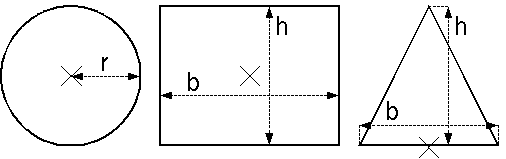
\includegraphics[height=1.8cm]{i1gem/shapes.png}
      % \caption{Formen}
      % \label{Formen}
    \end{center}
    % \end{figure}

  \item Es soll Funktionen geben, die auf allen Formen funktionieren
    und Folgendes leisten:

    \begin{itemize}

    \item kartesische Koordinate einer Form zurückgeben

    \item $x$-Koordinate einer Form zurückgeben

    \item $y$-Koordinate einer Form zurückgeben

    \item Abstand des Ursprungs einer Form zum Ursprung des
      Koordinatensystems zurückgeben

    \item Flächeninhalt einer Form zurückgeben

    \item Form um $\Delta_x$ in $x$-Richtung und um $\Delta_y$ in
      $y$-Richtung verschieben, also eine Form zurückgeben, deren
      Ursprungskoordinate entsprechend verschoben ist

%     \item Größe einer Form um einen Faktor ändern, also eine Form
%       zurückgeben, deren Größe entsprechend angepasst ist
  \item  Flächeninhalt zweier
    Formen vergleichen: Für gleich große Formen liefert die Prozedur
    \verb|"equal"| zurück, sonst \verb|"smaller"|, wenn die erste
    Form kleiner ist, beziehungsweise \verb|"bigger"|, wenn die erste
    Form größer ist.
    \end{itemize}

  \end{itemize}

  Zeigen Sie den Hackern, was richtiges Software-Engineering ist und
  benutzen Sie die passenden Konstruktionsanleitungen, um Repräsentationen für die Formen und die zugehörigen
  Funktionen zu schreiben!
\end{aufgabe}

\begin{aufgabe}

  Es gibt verschiedene Verstöße gegen die
  Straßenverkehrsordnung: 
  \begin{itemize}
  \item Falschparken mit Ort und Zeitpunkt des Verstoßes

  \item Überfahren einer roten Ampel mit Ort und Zeitpunkt des Verstoßes
    sowie der Dauer in Sekunden, wie lange die Ampel bereits rot war

  \item Überhöhte Geschwindigkeit mit Ort und Zeitpunkt des Verstoßes
    sowie der Höhe der Geschwindigkeits"-über"-tre"-tung
  \end{itemize}
  Neben den angegebenen Bestandteilen muss später für jeden Verstoß vermerkt 
  werden, ob zusätzlich eine "<Gefährdung des Straßenverkehrs"> vorliegt.
  
  \begin{enumerate}
  \item Schreiben Sie eine Datendefinition für
    Verstöße gegen die Straßenverkehrsordnung.  Schreiben Sie Daten-
    und Recorddefinitionen für die verschiedenen Verstöße.  Hinweis:
    Die Zeitpunkte können Sie durch Zeichenketten repräsentieren.  
    Geben Sie alle Signaturen an!

  \item Schreiben Sie eine Funktion, die einen
    beliebigen Verstoß entgegennimmt und den Ort des Verstoßes
    zurückgibt.

    Schreiben Sie analog eine Funktion, die einen
    beliebigen Verstoß entgegennimmt und den Zeitpunkt des Verstoßes
    zurückgibt.

  \item Schreiben Sie eine Funktion, die einen
    beliebigen Verstoß entgegennimmt, diesen als Gefährdung des
    Straßenverkehrs betrachtet und wieder zurückgibt (d.~h. jeder 
    Verstoß ist ein Verstoß mit Gefährdung).
  \end{enumerate}

  Die Verstöße haben unterschiedliche Tatbestände zur Folge:

  \begin{itemize}
  \item Einfaches Vergehen mit Bußgeld

  \item Ordnungswidrigkeit mit Bußgeld, Punkte für die
    Verkehrssünderdatei und Fahrverbot in Monaten

  \item Straftat mit Punkten für die Verkehrssünderdatei und
    Freiheitsstrafe in Monaten
  \end{itemize}
  
  \begin{enumerate} \setcounter{enumii}{3}
  \item Schreiben Sie eine Datendefinition für
    Tatbestände auf Verstöße gegen die Straßenverkehrsordnung.
    Schreiben Sie Daten- und Recorddefinitionen für die verschiedenen
    Tatbestände.  Geben Sie alle Signaturen an!

  \item Schreiben Sie eine Funktion, die einen
    beliebigen Tatbestand konsumiert und die Anzahl der anfallenden
    Punkte zurückliefert.
  \end{enumerate}

  Schreiben Sie nun Prozeduren, die Verstöße konsumieren und die
  Tatbestände berechnen:

  \begin{enumerate} \setcounter{enumii}{5}
  \item Schreiben Sie eine Funktion, die Falschparken
    konsumiert und ein einfaches Vergehen mit 20~Euro Bußgeld zurückgibt.
    Wenn das Falschparken eine Gefährdung des Straßenverkehrs
    darstellt (z.B.  bei Behinderung von Rettungsfahrzeugen),
    soll die Prozedur eine Ordnungswidrigkeit mit 40~Euro Bußgeld,
    einem Punkt und keinem Fahrverbot zurückgeben.

  \item Schreiben Sie eine Prozedur, die Überfahren
    einer roten Ampel konsumiert und eine Ordnungswidrigkeit
    zurückgibt.  Dabei gilt:
    \begin{itemize}
    \item wenn die Ampel kürzer als eine Sekunde rot war und keine
      Gefährdung vorlag: 50~Euro, 3~Punkte, kein Fahrverbot
    \item wenn die Ampel mindestens eine Sekunde rot war oder eine
      Gefährdung vorlag: 125~Euro, 4~Punkte, 1~Monat Fahrverbot
    \end{itemize}

  \item Schreiben Sie eine Prozedur, die überhöhte
    Geschwindigkeit konsumiert und den Tatbestand zurückgibt.  Dabei
    gilt:
    \begin{itemize}
    \item Geschwindigkeitsübertretung weniger als 20 km/h ohne Gefährdung:
      einfaches Vergehen mit 35~Euro
    \item Geschwindigkeitsübertretung zwischen 20 und 40 km/h
      (inklusive) ohne Gefährdung: Ordnungswidrigkeit mit 75~Euro,
      3~Punkten und 1~Monat Fahrverbot
    \item Geschwindigkeitsübertretung von mehr als 40 km/h ohne
      Gefährdung: Ordnungswidrigkeit mit 200~Euro, 4~Punkte und
      3~Monate Fahrverbot
    \item bei gleichzeitiger Gefährdung des Straßenverkehrs: Straftat
      mit 3~Punkte mehr als ohne Gefährdung angegeben und
      Freiheitsstrafe, die doppelt so lang ist wie das Fahrverbot, das
      ohne Gefährdung gilt (wenn es kein Fahrverbot gibt, dann gibt es
      auch keine Freiheitsstrafe)
    \end{itemize}

  \item Schreiben Sie eine Funktion, die einen
    Verstoß konsumiert und dessen Folge zurückgibt.  Benutzen Sie die
    Funktionen aus den vorherigen Teilaufgaben.
  \end{enumerate}
\end{aufgabe}


%%% Local Variables: 
%%% mode: latex
%%% TeX-master: "i1"
%%% End: 


% Diese Datei ist Teil des Buchs "Schreibe Dein Programm!"
% Das Buch ist lizensiert unter der Creative-Commons-Lizenz
% "Namensnennung - Weitergabe unter gleichen Bedingungen 4.0 International (CC BY-SA 4.0)"
% https://creativecommons.org/licenses/by-sa/4.0/deed.de

\chapter{Programmieren mit Selbstbezügen und Kombinatoren}
\label{cha:selbstbezug}

Zusammengesetzte und gemischte Daten sind die Hauptorganisationsformen
für Daten.  Allerdings haben wir bisher nur Daten vorgestellt, die
feste Größe haben und damit im Wortsinn beschränkt sind.  Viele
Informationen haben aber variable Größe: Die Bücher im Regal werden
immer mehr, Bauwerke bestehen aus variabel vielen Bauteilen.  Um
solche Informationen als Daten zu repräsentieren, stellen wir in
diesem Kapitel einen weiteren Aspekt der Datenanalyse vor, den
\textit{Selbstbezug}\index{Selbstbezug}.  Hier sind einfache
Beispiele:
%
\begin{itemize}
\item Ein Fluss besteht aus Hauptfluss und Nebenfluss~-- beides wieder
  Flüsse.
\item Ein Dateiverzeichnis auf dem Computer kann 
  Unterverzeichnisse enthalten.
\item Ein großer Bücherstapel besteht aus einem etwas kleineren
  Bücherstapel und einem weiteren Buch.
\end{itemize}
%
Bei all diesen Beispielen werden aus kleineren Dingen größere gemacht:
Aus zwei Flüssen, die zusammenfließen, wird ein großer Fluss.  Aus
mehreren Dateien und Verzeichnissen wird ein großes Verzeichnis.  Aus
einem kleinen Bücherstapel wird ein großer.  In der Programmierung
nennen wir das Bauen von großen Dingen aus kleinen Dingern derselben
Sorte \textit{kombinieren}. Die Funktionen, die das erledigen, heißen
\textit{Kombinatoren}\index{Kombinator}: Um die geht es in diesem Kapitel.

\section{Flüsse abbilden}

\begin{figure}[tbh]
  \centering
\begin{tikzpicture}
  [
    confluence/.style = {shape=rectangle, rounded corners,
                         draw, align=center},
    absent/.style = {},
    grow                    = left,
    sibling distance        = 6em,
    level distance          = 10em,
    % makes arrows the opposite direction from -latex
    edge from parent/.style = {draw,latex-},
    every node/.style       = {font=\footnotesize}
    ]
    \node [absent] {}
    child {
      node [confluence] {Epfendorf}
        child {
          node [confluence] {Tieringen}
          edge from parent node [below] {Schlichem} }
        child { node  [confluence] {Rottweil}
          child { node [confluence] {Heimliswald}
            edge from parent node [below] {Eschach} }
          child { node [confluence] {Dreifaltigkeitsberg}
            edge from parent node [below] {Prim} } } };
\end{tikzpicture}
  \caption{Der Neckar nahe der Quellen}
  \label{fig:neckar}
\end{figure}

\noindent Abbildung~\ref{fig:neckar} ist ein Diagramm, das die
Struktur des Neckar nahe der Quellen beschreibt: Er fließt zunächst
aus den Bächen Eschach und Prim zusammen, und danach fließen immer
weitere Bäche und Flüsse hinzu~-- in der Abbildung noch die
Schlichem.

Die Struktur eines Flusses werden wir durch Daten abbilden, um danach
eine Funktion zu schreiben, die feststellt, ob ein Fluss durch einen
bestimmten Ort fließt.  Unser erster Versuch einer Datendefinition
sieht so aus:
%
\begin{lstlisting}
; Ein Fluss kommt entweder aus:
; - einer Quelle
; - einem Hauptfluss und einem Nebenfluss
\end{lstlisting}
%
Man kann zwar schon sehen, dass es sich um eine Fallunterscheidung
handelt, aber wir können die Formulierung schärfen, um klar zu machen,
dass es sich um gemischte Daten handelt:
%
\begin{lstlisting}
; Ein Fluss ist eins der folgenden:
; - ein Bach aus einer Quelle
; - ein Zusammentreffen von einem Hauptfluss und einem Nebenfluss
\end{lstlisting}
%
Daraus können wir direkt eine Signaturdefinition machen:
%
\begin{lstlisting}
(define river
  (signature (mixed creek confluence)))
\end{lstlisting}
%
Die Datendefinitionen für "<Bach"> und "<Zusammentreffen"> fehlen
allerdings noch.  In Abbildung~\ref{fig:neckar} steht an den Bächen
jeweils noch der Name.  Eine passende Datendefinition sieht so aus:
%
\begin{lstlisting}
; Ein Bach hat folgende Eigenschaften:
; - Ursprungsort
\end{lstlisting}
%
Das klingt ein bißchen komisch, weil der Bach ja nur \emph{eine}
Eigenschaft hat, aber die Datendefinition trotzdem zusammengesetzte
Daten beschreibt.  Trotzdem ist das legitim und korrekt~-- niemand
wird sagen wollen, dass der Ursprungsort der Bach \emph{ist}.
Außerdem kannst Du Dir vorstellen, dass ein Bach später noch mehr
Eigenschaften bekommt, die wir in den Daten festhalten
wollen. (Wasserqualität oder Fließgeschwindigkeit zum Beispiel.)
Entsprechend ist es auch sinnvoll, dafür eine Record-Definition zu
schreiben:
%
\begin{lstlisting}
(define-record-functions creek
  make-creek
  creek?
  (creek-origin string))
\end{lstlisting}
%
Wenn später noch weitere Eigenschaften hinzukommen, können wir die
Record-Definition erweitern, ohne anderen Code zu beeinträchtigen.

Kommen wir zu den Zusammentreffen.  Auch hier ist ein Ort relevant~--
dort, wo sie zusammentreffen.  Außerdem ist wichtig, \emph{welche}
Flüsse oder Bäche da zusammentreffen.  Die Datendefinition könnte so
aussehen:
%
\begin{lstlisting}
; Ein Zusammentreffen besteht aus:
; - Ort
; - Hauptfluss
; - Nebenfluss
\end{lstlisting}
%
Die Formulierung zeigt eindeutig, dass es sich um zusammengesetzte
Daten handelt.  Aber diese Datendefinition weist eine Auffälligkeit
auf, die erst sichtbar wird, wenn wir sie im Zusammenhang der
Gesamt-Datendefinition für Flüsse betrachten:
%
\tikzstyle{every picture}+=[remember picture]
\tikzstyle{fluss} = [shape=rectangle,inner sep=0pt,text depth=0pt]
%
\begin{lstlisting}
; Ein |\tikz\node[fluss](fluss){\textbf{Fluss}};| ist eins der folgenden:
; - |\ldots|
; - ein Zusammentreffen |\ldots|
|\ldots|
; Ein Zusammentreffen besteht aus:
; - Ort
; - Haupt|\tikz\node[fluss](fluss1){\textbf{fluss}};|
; - Neben|\tikz\node[fluss](fluss2){\textbf{fluss}};|
\end{lstlisting}
%
\begin{tikzpicture}[overlay]
  \path[->,blue,thick](fluss1) edge [out=0, in=0] (fluss);
  \path[->,blue,thick](fluss2) edge [out=0, in=0] (fluss);
\end{tikzpicture}
%
Die Datendefinition für "<Fluss"> benutzt selbst den Begriff
"<Fluss">.   Noch offensichtlicher wird das, wenn wir die dazu
passende Record-Definition erstellen:
%
\begin{lstlisting}
(define-record-functions confluence
  make-confluence
  confluence?
  (confluence-location  string)
  (confluence-main-stem river)
  (confluence-tributary river))
\end{lstlisting}
%
In der Definition von \texttt{confluence} wird \texttt{river} benutzt
und umgekehrt.  Das ist nichts schlimmes~-- im Gegenteil, diese beiden
\textit{Selbstbezüge}\index{Selbstbezug} erlauben uns, ganz
unterschiedliche Flüsse zu beschreiben, insbesondere solche
unterschiedlicher Größe.  Den Abschnitt des Neckar in~\ref{fig:neckar}
können wir so abbilden:
%
\begin{lstlisting}
(define eschach (make-creek "Heimliswald")) ; Quelle des Neckar
(define prim (make-creek "Dreifaltigkeitsberg")) ; Quelle des Neckar
; erster Zusammenfluss des Neckar:
(define neckar-1 (make-confluence "Rottweil" eschach prim))
; Zufluss des Neckar:
(define schlichem (make-creek "Tieringen")) 
; zweiter Zusammenfluss des Neckar:
(define neckar-2 (make-confluence "Epfendorf" neckar-1 schlichem))
\end{lstlisting}
%
An diesen Beispielen sieht man sehr schön, dass
\texttt{make-confluence} zwei Flüsse zu einem kombiniert~-- es handelt
sich um einen \textit{Kombinator}\index{Kombinator}.

Wir hatten angekündigt, eine Funktion zu schreiben, die feststellt, ob
ein Fluss durch einen bestimmten Ort fließt.  Wir machen das wieder
nach Vorschrift, also zuerst die Kurzbeschreibung:
%
\begin{lstlisting}
; Fließt Fluss durch den angegebenen Ort?
\end{lstlisting}
%
In der Kurzbeschreibung sind schon die Substantive "<Fluss"> und
"<Ort"> als Eingaben aufgeführt, die übertragen wir in die Signatur.
Da die Funktion eine Ja-/Nein-Frage beantwortet, liefert sie einen
booleschen Wert und hat ein Fragezeichen hinten am Namen:
%
\begin{lstlisting}
(: flows-through? (river string -> boolean))
\end{lstlisting}
%
Bei den Tests achten wir darauf, dass wir sowohl Bäche als auch Flüsse
testen, und sowohl Fälle, bei denen \lstinline{#t} als auch solche,
bei denen \lstinline{#f} herauskommt:
%
\begin{lstlisting}
(check-expect (flows-through? eschach "Heimliswald") #t)
(check-expect (flows-through? eschach "Tübingen") #f)
(check-expect (flows-through? neckar-2 "Heimliswald") #t)
(check-expect (flows-through? neckar-2 "Rottweil") #t)
(check-expect (flows-through? neckar-2 "Berlin") #f)
\end{lstlisting}
%
Das Gerüst ergibt sich wie immer direkt aus der Signatur:
%
\begin{lstlisting}
(define flows-through?
  (lambda (river location)
    ...))
\end{lstlisting}
%
Da es sich bei \lstinline{river} um gemischte Daten handelt, können
wir die Schablone dafür ergänzen.  Da \lstinline{river} zwei Fälle hat
(Bäche und Zusammenflüsse), muss die Schablone zwei Zweige haben.  Die
Bedingungen sind Aufrufe der jeweiligen Prädikate für
\lstinline{creek} und \lstinline{confluence}:
%
\begin{lstlisting}
(define flows-through?
  (lambda (river location)
    (cond
      ((creek? river) ...)
      ((confluence? river) ...))))
\end{lstlisting}
%
Nun können wir Code für die beiden Zweige ergänzen.  Fangen wir mit
den Bächen an.  Da es sich bei \lstinline{creek} um zusammengesetzte
Daten handelt (mit nur einem Bestandteil), sollte der Aufruf des
Selektors im Rumpf vorkommen:
%
\begin{lstlisting}
(define flows-through?
  (lambda (river location)
    (cond
      ((creek? river)
       ... (creek-origin river) ...
      ((confluence? river)
       ...))))
\end{lstlisting}
%
Der Selektor \lstinline{creek-origin} hat einen Ursprungsort.  Wenn dieser dem
gesuchten Ort entspricht, so fließt der Fluss durch diesen Ort, sonst
nicht.  Im ersten Fall sollte \lstinline{#t} herauskommen, im zweiten
\lstinline{#f}.  Das sieht so aus:
%
\begin{lstlisting}
(define flows-through?
  (lambda (river location)
    (cond
      ((creek? river)
       (if (string=? (creek-origin river) location)
           #t
           #f))
      ((confluence? river)
       ...))))
\end{lstlisting}
%
Dieser Code kann noch etwas vereinfacht werden: Der
\lstinline{if}-Ausdruck sagt ja salopp formuliert:
%
\begin{quote}
  Wenn \lstinline{(string=? (creek-origin river) location)} als
  Resultat \lstinline{#t} liefert, dann \lstinline{#f}, und wenn es
  \lstinline{#f} liefert, dann \lstinline{#f}.
\end{quote}
%
Da reicht es auch, \lstinline{(string=? (creek-origin river) location)} hinzuschreiben.
%
\begin{aufgabe}\label{aufgabe:iftruefalse}
  Kannst Du diese Vereinfachung auf \lstinline{if}-Ausdrücken
  verallgemeinern und als Gleichung schreiben?
\end{aufgabe}
%
Als nächstes können wir uns um den anderen Fall kümmern,
\lstinline{confluence}.  Auch dort handelt es sich um
zusammengesetzte Daten, wir können also schon einmal die
Selektoraufrufe hinschreiben:
%
\begin{lstlisting}
(define flows-through?
  (lambda (river location)
    (cond
      ((creek? river)
       (string=? (creek-origin river) location))
      ((confluence? river)
      ...
       (confluence-location river)
       (confluence-main-stem river)
       (confluence-tributary river)
       ...))))
\end{lstlisting}
%
Soweit die Schablone, wir können uns also Gedanken zur eigentlichen
Aufgabe machen.

Als erstes steht da \lstinline{(confluence-main-stem river)} der Ort
des Zusammenflusses.  Wenn es sich dabei um den gesuchten Ort handelt,
können wir die Frage, ob der Fluss durch diesen Ort fließt, bereits
mit "<ja"> beziehungsweise \lstinline{#t} beantworten:
%
\begin{lstlisting}
(define flows-through?
  (lambda (river location)
    (cond
      ((creek? river)
       (string=? (creek-origin river) location))
      ((confluence? river)
       (if (string=? (confluence-location river) location)
           #t
           ...
           (confluence-main-stem river)
           (confluence-tributary river)
           ...)))))
\end{lstlisting}
%
Aber was wenn nicht?  Dann müssen wir uns an die beiden anderen
Selektor-Aufrufe halten, die uns den Haupt- und den Nebenfluss des
Zusammenflusses liefern.  Wenn der eine oder der andere durch den
gesuchten Ort fließt, dann könnten wir die Frage unserer Funktion
ebenfalls mit "<ja"> beantworten.  Dazu müssten wir also feststellen:
%
\begin{enumerate}
\item Fließt der Hauptfluss durch den Ort \lstinline{origin}?
\item Fließt der Nebenfluss durch den Ort \lstinline{origin}?
\end{enumerate}
%
Nun, wir schreiben ja gerade eine Funktion, die feststellt, ob ein
Fluss durch einen bestimmten Ort fließt.  Können wir die benutzen?
Wir schreiben das mal hin:
%
\begin{lstlisting}
(define flows-through?
  (lambda (river location)
    (cond
      ((creek? river)
       (string=? (creek-origin river) location))
      ((confluence? river)
       (if (string=? (confluence-location river) location)
           #t
           ...
           (flows-through? (confluence-main-stem river) location)
           (flows-through? (confluence-tributary river) location)
           ...)))))
\end{lstlisting}
%
Die beiden Aufrufe von \lstinline{flows-through?} entsprechen gerade
den beiden Fragen von oben.  Wir können ihre Ergebnisse kombinieren,
um unsere Antwort zu errechnen: Wenn der Hauptfluss durch
\lstinline{location} fließt \emph{oder} der Nebenfluss durch
\lstinline{location} fließt, so fließt auch der "<Gesamtfluss"> durch
\lstinline{location}.  So sieht das aus:
%
\begin{lstlisting}
(define flows-through?
  (lambda (river location)
    (cond
      ((creek? river)
       (string=? (creek-origin river) location))
      ((confluence? river)
       (if (string=? (confluence-location river) location)
           #t
           (or
            (flows-through? (confluence-main-stem river) location)
            (flows-through? (confluence-tributary river) location)))))))
\end{lstlisting}
%
Fertig!

In dieser Funktion passiert etwas besonderes, das es in den
Funktionen davor noch nicht gab: Sie enthält einen Aufruf von sich
selbst, einen sogenannten \textit{rekursiven Aufruf\index{rekursiver
    Aufruf}}.  Diese rekursiven Aufrufe sind genau an den Stellen, wo
die Datendefinition von \lstinline{river} Selbstbezüge enthält.

Das ist kein Zufall: Nahezu alle Funktionen, die Daten mit
Selbstbezügen konsumieren, enthalten an den Stellen der Selbstbezüge
rekursive Aufrufe.  Daraus machen wir eine Schablone:
%
\begin{konstruktionsanleitung}{Selbstbezüge als Eingabe: Schablone}
  \label{ka:selbstbezug-schablone}
  Wenn Du eine Funktion schreibst, die Daten konsumiert, in denen
  Selbstbezüge enthalten sind, dann schreibe an die Stellen der
  Selbstbezüge jeweils einen rekursiven Aufruf.
\end{konstruktionsanleitung}
%
Ein Nachtrag noch: Der \lstinline{if}-Ausdruck in der
\lstinline{flows-through?}-Funktion passt \emph{fast} auf das Muster
aus Aufgabe~\ref{aufgabe:iftruefalse}.  Der einzige Unterschied ist,
dass in der Alternative der Verzweigung nicht \lstinline{#f} steht.
Allgemein wir ein solcher \lstinline{if}-Ausdruck folgendermaßen
ausgewertet:
%
\begin{lstlisting}
(if |$b$| #t |$a$|)
|\evalsto| #t ; falls |$b=$| #t
|\evalsto| |$a$|  ; falls |$b=$| #f
\end{lstlisting}
%
Das können wir mit dem Verhalten von \lstinline{or} vergleichen:
%
\begin{lstlisting}
(or |$b$| |$a$|)
|\evalsto| #t ; falls |$b$| |\evalsto| #t
|\evalsto| |$a$|  ; falls |$b$| |\evalsto| #f
\end{lstlisting}
%
Wir können den \lstinline{if}-Ausdruck aus \lstinline{flows-through?}
also durch ein \lstinline{or} ersetzen:
%
\begin{lstlisting}
         (or (string=? (confluence-location river) location)
             (or
              (flows-through? (confluence-main-stem river) location)
              (flows-through? (confluence-tributary river) location)))
\end{lstlisting}
%
Das können wir sogar noch weiter vereinfachen, weil \lstinline{or}
auch mit drei Operanden funktioniert:
%
\begin{lstlisting}
         (or (string=? (confluence-location river) location)
             (flows-through? (confluence-main-stem river) location)
             (flows-through? (confluence-tributary river) location))
\end{lstlisting}
%
Wenn wir das Resultat, steht da folgendes:
%
\begin{quote}
  Der Zusammenfluss \lstinline{river} fließt durch
  \lstinline{location}, wenn

  \begin{itemize}
  \item der Zusammenfluss gerade bei \lstinline{location} stattfindet

    \centerline{\textbf{oder}}
  \item der Hauptfluss durch \lstinline{location} fließt

    \centerline{\textbf{oder}}
  \item der Nebenfluss durch \lstinline{location} fließt.
  \end{itemize}
\end{quote}
%
So erzählt ist die Funktionsweise von \lstinline{flows-through?}
(hoffentlich) direkt verständlich.

Wir können so aus diesem Beispiel und
Aufgabe~\ref{aufgabe:iftruefalse} zwei Gleichungen entsprechend
Mantra~\ref{mantra:gleichungen} auf Seite~\pageref{mantra:gleichungen}
machen:
%
\begin{lstlisting}
(if |$b$| #t #f) |$=$| |$b$|
(if |$b$| #t |$a$|)  |$=$| (or |$b$| |$a$|)
\end{lstlisting}
%

\section{Bilder modellieren}

FIXME: Kombinatoren \texttt{overlay}, \texttt{beside}, \texttt{above}


FIXME: Kombinator erkennen an der Signatur

FIXME: andere Signatur für \texttt{make-confluence}

\section{Finanzverträge abbilden}

Es ist Zeit für ein etwas größeres Beispiel.  Wir bilden
Finanzverträge ab und programmieren dazu eine stark vereinfachte
Version eines Klassikers der Informatik-Forschung, das zu mehreren
Veröffentlichungen und zur Gründung einer erfolgreichen Firma geführt
hat.\footnote{Wer mehr wissen möchte, sollte das Paper von Peyton
  Jones und Eber~\cite{FinancialContracts} lesen, das es auch im
  Internet zum Download gibt.}  Selbstbezüge spielen eine wichtige
Rolle.

Wichtig bei diesem Beispiel: Für die Repräsentation von
Finanzverträgen aus diesem Abschnitt haben renommierte
Informatik-Forscher mehrere Monate gebraucht.  Wir können sie mit den
bisher präsentierten Programmiermitteln nachbauen, aber Du solltest
nicht von Dir erwarten, dass Du das Beispiel in wenigen Stunden auch
selbst hättest ausdenken können.

In der Finanzbranche werden oft Verträge geschlossen, die zur
strukturierten Zahlung von Geldbeträgen führen.  Wer eine Bankerin
fragt, was der einfachste solche Vertrag ist, bekommt oft die Antwort
\textit{Zero-Bond}.  Hier ist ein Beispiel für einen Zero-Bond:
%
\begin{center}
  Ich bekomme am 31.\ Juni 2030 \EUR{1000}.
\end{center}
%
So ein Vertrag wird immer zwischen zwei Vertragspartnern geschlossen und der
eine ist immer "<ich">.  Daher kommt die Formulierung "<Ich
bekomme">.  Der Begriff "<Zero-Bond"> setzt sich zusammen aus "<keine
Zinsen"> (Zero) und "<Recht auf spätere Zahlung"> (Bond).

Wir können daraus eine einfache Datendefinition machen:
%
\begin{lstlisting}
; Ein Zero-Bond hat folgende Eigenschaften:
; - Datum
; - Betrag
; - Währung
\end{lstlisting}
%
An der Formulierung "<hat folgende Eigenschaften"> sehen wir sofort,
dass es sich um zusammengesetzte Daten handelt.  Daraus folgt direkt
diese Reocrd-Definition:
%
\begin{lstlisting}
(define-record-functions zero-bond
  make-zero-bond
  (zero-bond-date     date)
  (zero-bond-amount   rational)
  (zero-bond-currency currency))
\end{lstlisting}
%
Wir müssten noch Definitionen für \texttt{date} und \texttt{currency}
beisteuern, schieben das aber auf die lange Bank.  Wir wollen
stattdessen zunächst noch einmal grundsätzlich über die richtige
Datendefinition für solche Verträge nachdenken.

Es gibt ja noch viel mehr solche Verträge: Futures, Forwards, Swaps,
Swaptions~\ldots{} Jeder Vertrag hat mehrere Eigenschaften, das würde
also darauf hinauslaufen, dass wir sehr viele Datendefinitionen für
zusammengesetzte Daten und die zugehörigen Record-Definitionen
schreiben müssten~-- und am Ende eine Datendefinition zu "<Vertrag">,
die auf eine große Signatur für gemischte Daten hinausläuft.  Das ist
eine Menge Arbeit, und sie wäre auch nie fertig, weil sich die Banker
ständig neue Verträge ausdenken.

Wer aber genug solche Verträge studiert, bemerkt, dass diese aus
Bausteinen bestehen, die immer wiederkehren.  Das suggeriert einen
anderen Ansatz, nämlich diese Bausteine zu identifizieren und dafür
die Datenanalyse durchzuführen.  Wir nachvollziehen stattdessen der
Arbeit der Autoren des Papers~\cite{FinancialContracts}.  Die haben
(über mehrere Monate) einen Satz bestechend einfacher Bausteine
zusammengestellt, indem sie bekannte Verträge in möglichst kleine und
einfache Bestandteile zerlegten.  Jeder dieser Bestandteile ist für
sich genommen ein "<kleiner Vertrag">, es gibt aber auch Kombinatoren,
die aus kleinen Verträgen größere machen, insbesondere auch noch
unbekannte Klassen von Verträgen.  Aus diesen Bestandteilen lassen sich
sehr viele Finanzverträge (auch noch unbekannte) abbilden durch den
Einsatz von Kombinatoren.

Da es mehrere Klassen von Bausteinen und Kombinatoren gibt, werden wir
Verträge als gemischte Daten repräsentieren und dafür schrittweise
eine Datendefinition folgender Form aufbauen:
%
\begin{lstlisting}
; Ein Vertrag ist eins der folgenden:
; - ...
\end{lstlisting}
%
Dazu gehört natürlich eine passende Signaturdefinition, die wir
ebenfalls schrittweise aufbauen werden:
%
\begin{lstlisting}
(define contract
  (signature (mixed |\ldots|)))
\end{lstlisting}
%
Um die Bausteine und Kombinatoren zu identifizieren, schauen wir uns
zunächst den Zero-Bond näher an.  Auch wenn der einfach aussieht, gibt
es mehrere Aspekte, die auch unabhängig voneinander Sinn ergeben: die
Auszahlung eines bestimmten \textit{Betrags} in einer bestimmten
\textit{Währung} und die Möglichkeit, eine Zahlung \textit{später} zu
veranlassen.  Das sind drei separate Ideen, und es ist sinnvoll, diese
getrennt als Daten zu repräsentieren.

\paragraph{Zahlung einer bestimmten Währung}
Fangen wir an mit der Zahlung einer bestimmten Währung.  Der
Einfachheit halber nehmen wir an, dass alle Zahlungen in Euro sind.
Um die richtige Daten-Definition zu finden, versuchen wir, die
\emph{einfachste} Euro-Zahlung zu finden, und die besteht aus
\emph{einem} Euro.  Die Daten-Definition dazu ist ernüchternd einfach:
%
\begin{lstlisting}
; Ein Euro hat keine Eigenschaften
\end{lstlisting}
%
Wir könnten den Euro einfach als die Zeichenkette \lstinline{"EUR"}
abbilden.  Das wäre sinnvoll, wenn der Euro Teil einer Aufzählung ist.
Dies ist allerdins hier nicht der Fall, andere Vertragsbausteine haben
durchaus Eigenschaften.  (Siehe dazu auch
Aufgabe~\ref{aufgabe:aufzaehlung-vs-nullstellig} auf
Seite~\pageref{aufgabe:aufzaehlung-vs-nullstellig}.)  Wir nehmen die
Datendefinition stattdessen beim Wort "<hat~\ldots{} Eigenschaften">
und bilden den Euro als zusammesngesetzte Daten ab.  Dann wird daraus
folgende Record-Definition:
%
\begin{lstlisting}
(define-record-functions one-euro
  make-one-euro
  one-euro?)
\end{lstlisting}
%
Wir fügen als nächstes \lstinline{one-euro} zur Daten- und zur
Signaturdefinition von \lstinline{contract} hinzu:
%
\begin{lstlisting}
; Ein Vertrag ist eins der folgenden:
; - ein Euro
; - ...
(define contract
  (signature (mixed one-euro |\ldots|)))
\end{lstlisting}
%
\paragraph{Beliebige Beträge}
Als nächstes bilden wir die Möglichkeit ab, einen Betrag zu wählen.
Eine naheliegende erste Idee wäre, die Idee "<$n$ Euros"> abzubilden,
etwa so:
%
\begin{lstlisting}
; Euros haben folgende Eigenschaft:
; - wieviele
(define-record-functions euros
  make-euros
  euros?
  (euros-amount rational))
\end{lstlisting}
%
Wenn wir das hätten, bräuchten wir aber \lstinline{one-euro} nicht mehr.
Außerdem wäre das Resultat dann nicht mehr so einfach wie möglich:
Besser wäre es, wenn wir die Idee "<wieviele"> trennen könnten von
"<Euro">.  Dann könnten wir sagen "<mehrere von einem Euro">.  Das
klingt erstmal komisch, auch in der Datendefinition:
%
\begin{lstlisting}
; Mehrere haben folgende Eigenschaften:
; - wieviele
; - wovon
\end{lstlisting}
%
Aber die richtige Form für zusammengesetzte Daten hat das schon
einmal.  Es reicht für eine erste Skizze einer Record-Definition:
%
\begin{lstlisting}
(define-record-functions multiple
  make-multiple
  multiple?
  (multiple-number |\ldots|)
  (multiple-of     |\ldots|))
\end{lstlisting}
%
Wir müssen aber noch klären, was die Signatur von
\lstinline{multiple-number} respektive \lstinline{multiple-of} ist.
Bei \lstinline{multiple-number} müssen wir uns nicht auf ganze Zahlen
beschränken~-- ein halber Euro geht schließlich auch.  Da ist
\lstinline{rational} sinnvoll.

Bei \lstinline{multiple-of} liegt es nahe, \lstinline{one-euro}
hinzuschreiben: Dann könnten wir den Zero-Bond schon hinschreiben.
Allerdings wäre \lstinline{multiple} ziemlich eingeschränkt und nicht
besonders zukunftssicher: Was, wenn andere Währungen dazukommen,
\lstinline{one-gbp} oder so?  Vielleicht sind wir versucht, eine
Signatur \lstinline{currency} für Währungen zu definieren und für
\lstinline{multiple-of} zu verwenden.  Aber das wäre immer noch zu
eingeschränkt: Man kann ja auch mehrere Aktien (zum Beispiel) im
Rahmen eines Vertrags übergeben~-- oder auch mehrere Zero-Bonds oder
andere Verträge.

Und da ist sie ganz plötzlich, die zentrale Idee: Dass ein Vertrag den
Abschluss \emph{anderer} Verträge verfügen kann.  Wir schreiben
deshalb als Signatur von \lstinline{multiple-of} einfach
\lstinline{contract} und schärfen bei der Gelegenheit die Datendefinition:
%
\begin{lstlisting}
; Ein Vielfaches besteht aus:
; - Anzahl
; - Vertrag 
(define-record-functions multiple
    make-multiple
    multiple?
    (multiple-number rational)
    (multiple-of     contract))
\end{lstlisting}
%
Nun gibt es schon zwei Klassen Verträge~-- \lstinline{one-euro} und
\lstinline{multiple}.  Wir erweitern die Definition von
\lstinline{contract} entsprechend:
%
\begin{lstlisting}
(define contract
  (signature (mixed one-euro multiple)))
\end{lstlisting}
%
Mit Hilfe von \lstinline{one-euro} und \lstinline{multiple} können wir
einen Vertrag definieren, der festlegt, dass wir \EUR{100} bekommen~--
sofort:
%
\begin{lstlisting}
(define euro100 (make-multiple 100 (make-one-euro))) ; 100 Euros
\end{lstlisting}
%
\begin{aufgabe}
  Definiere eine Funktion \lstinline{make-euros} mit Kurzbeschreibung,
  Signatur und Test wie folgt:
\begin{lstlisting}
; Euro-Betrag auszahlen
(: make-euros (rational -> contract))

(check-expect (make-euros 100) euro100)
\end{lstlisting}
\end{aufgabe}
%
Mit Hilfe der Funktion aus der Aufgabe können wir leicht auch
\EUR{200} definieren:
%
\begin{lstinline}
(define euro200 (make-euros 200)) ; 200 Euros
\end{lstinline}

\paragraph{Verzögerungen}
Für die Zero-Bonds benötigen wir noch die Möglichkeit,
eine Zahlung zu verzögern.
Dazu benutzen wir den gleichen Trick wie
bei \lstinline{multiple} und definieren einen weiteren Kombinator, der
einen ganzen Vertrag verzögert: Wir schließen also einen Vertrag ab,
später einen Vertrag abzuschließen, und der kann dann die Zahlung
auslösen.  Um so einen Vertrag zu beschreiben, benötigen wir das
Datum, an dem der "<spätere"> Vertrag aktiv wird und den späteren
Vertrag selbst:
%
\begin{lstlisting}
; Eine Verzögerung besteht aus:
; - Datum
; - Vertrag, der zu dem Datum gültig wird
\end{lstlisting}
%
Diese Datendefinition beschreibt wieder zusammengesetzte Daten.  Die
dazugehörige Record-Definition sieht so aus:
%
\begin{lstlisting}
(define-record-functions later
  make-later
  later?
  (later-date     date)
  (later-contract contract))
\end{lstlisting}
%
Mit \lstinline{later} können wir die Signatur-Definition von
\lstinline{contract} erweitern:
%
\begin{lstlisting}
(define contract
  (signature (mixed one-euro multiple later)))
\end{lstlisting}
%
Aber es fehlt noch etwas: Wir haben für \lstinline{later-date} die
Signatur \lstinline{date} verwendet, die noch gar nicht definiert ist.
Die Definition von \texttt{date} liegt zum Glück recht nahe:
%
\begin{lstlisting}
(define-record-functions date
  make-date
  date?
  (date-year  natural)
  (date-month natural)
  (date-day   natural))
\end{lstlisting}
%
\begin{aufgabe}
  Wir haben für alle Felder von \lstinline{date} die Signatur
  \lstinline{natural} verwendet. Diese Signatur ist sehr unpräzise.
  Eine Möglichkeit, sie zu verbessern ist, eine
  \textit{Prädikat-Signatur}\index{Prädikat-Signatur} zu definieren.
  Dafür brauchen wir ein Prädikat, das einen korrekten Monat
  identifiziert:
  %
\begin{lstlisting}
; Bezeichnet eine Zahl einen Monat?
(: month? (natural -> boolean))

(check-expect (month? 1) #t)
(check-expect (month? 6) #t)
(check-expect (month? 12) #t)
(check-expect (month? 0) #f)
(check-expect (month? 13) #f)

(define month?
  (lambda (n)
    (and (>= n 1)
         (<= n 12))))  
\end{lstlisting}
  %
  Mit diesem Prädikat können wir eine Signatur definieren, die genau
  dann passt, wenn das Prädikat \lstinline{#t} liefert.  Dazu benutzen
  einen neues Konstruktor für Signaturen, \lstinline{predicate}\index{predicate@\texttt{predicate}}:
\begin{lstlisting}
(define month (signature (predicate month?)))
\end{lstlisting}
%
  Ändere die Definition von \lstinline{date}, so dass sie
  \lstinline{month} benutzt!  Mache eine entsprechende Änderung für
  \lstinline{date-day}!
\end{aufgabe}
%
Bevor es weitergeht, definieren wir noch zwei Beispiele für das Datum:
%
\begin{lstlisting}
(define date1 (make-date 2019 07 26)) ; 26. Juli 2019
(define date2 (make-date 2019 12 24)) ; Weihnachten 2019
\end{lstlisting}
%
Mit Hilfe dieser Definitionen können wir auch endlich zwei Beispiele
für \lstinline{later} angeben:
%
\begin{lstlisting}
(define later1 (make-later date1 euro100)) ; Ich bekomme Neujahr 2020 100|\EUR{}|.
(define later2 (make-later date2 euro200)) ; Ich bekomme am 27.7.2019 200|\EUR{}|.
\end{lstlisting}
%
Außerdem können wir den Zero-Bond vom Anfang dieses Abschnitts
definieren:
%
\begin{lstlisting}
; Ich bekomme am 31. Juni 2030 1000|\EUR{}|.
(define zero1 (make-later (make-date 2030 06 31)
                          (make-euros 1000)))
\end{lstlisting}

\begin{figure}[tb]
  \centering
\begin{tikzpicture}
  \draw [fill=gray!50] (0, 0) rectangle (10, 4);
  \draw [fill=gray!75] (0.5, 0.5) rectangle (9.5, 3);
  \draw [fill=gray] (1, 1) rectangle (8, 2);
  \node [right] at (0.5, 3.5) {\lstinline{later}};
  \node at (5, 3.5) {\lstinline{"31.6.20230"}};
  \node [right] at (1, 2.5) {\lstinline{multiple}};
  \node at (5, 2.5) {\lstinline{1000}};
  \node [right] at (1.5, 1.5) {\lstinline{one-euro}};
\end{tikzpicture}
  
  \caption{Zero-Bond als Schichten dargestellt}
  \label{fig:zero-bond}
\end{figure}

\noindent Abbildung~\ref{fig:zero-bond} zeigt den Aufbau des
Zero-Bonds \lstinline{zero1} als ineinandergeschachtelte Schichten:
In den \lstinline{later}-Vertrag ist ein \lstinline{multiple}-Vertrag
eingeschachtelt, und dort wiederum der \lstinline{one-euro}-Vertrag.
Aus dieser Sicht ist der \lstinline{multiple}-Vertrag der
"<innere"> Vertrag des \lstinline{later}-Vertrags.

\paragraph{Verträge kombinieren}

Jetzt wo die Zero-Bonds erledigt sind, können wir überlegen, ob es
noch weitere Möglichkeiten geben sollte, Verträge herzustellen.  Wann
immer Du Repräsentationen mit Kombinatoren baust, solltest Du nach
Möglichkeiten suchen, aus zwei Dingen ein größeres Ding zu bauen.

Beispiele für dieses Prinzip haben wir in diesem Kapitel schon mehrere
gesehen:
%
\begin{itemize}
\item Ein Hauptfluss und ein Nebenfluss werden zu einem Fluss
  kombiniert.
\item Zwei Bilder werden übereinander, nebeneinander und aufeinander
  zu einem Bild kombiniert.
\end{itemize}
%
Auf die Verträge bezogen bedeutet dies, dass wir zwei Verträge
zusammensetzen, der die Rechte und Pflichten von beiden kombiniert.
So könnte dies gehen:
%
\begin{lstlisting}
; Eine Kombinationsvertrag besteht aus:
; - Vertrag Nr. 1
; - Vertrag Nr. 2
\end{lstlisting}
%
Das sind wieder zusammengesetzte Daten mit zwei Selbstbezügen:
%
\begin{lstlisting}
(define-record-functions both
  make-both
  both?
  (both-contract-1 contract)
  (both-contract-2 contract))
\end{lstlisting}
%
Hier sind zwei Beispiele für \lstinline{both}:
%
\begin{lstlisting}
; Heute 100|\EUR{}|, später nochmal 100|\EUR{}|
(define both1 (make-both euro100 later1))
; Heute 200|\EUR{}|, später nochmal 200|\EUR{}|
(define both2 (make-both both1 later2))
\end{lstlisting}
%
Wir müssen noch die Definition von \lstinline{contract} erweitern:
%
\begin{lstlisting}
(define contract
  (signature (mixed one-euro multiple later both)))
\end{lstlisting}
%

\paragraph{Der kleinste Vertrag}

Es gibt noch ein weiteres Prinzip beim Repräsentieren mit
Kombinatoren: Suche immer nach dem \emph{kleinsten} möglichen
Baustein.  Wir haben ja schon einen ziemlich kleinen Baustein
definiert: \lstinline{one-euro}.  Aber oft ist der kleine Baustein
eine Variation von "<nichts">, und so ist es auch hier: Der kleinste
Vertrag ist einer ohne Rechte oder Pflichten.  Ihn sollten wir
unbedingt auch definieren~-- zunächst nur der Vollständigkeit halber,
aber später werden wir ihn tatsächlich noch brauchen.

Solch ein "<Nichts-Vertrag"> hat, wie \lstinline{one-euro} auch, keine
Eigenschaften.  Wir repräsentieren ihn aber, genau wie bei
\lstinline{one-euro}, durch einen Record, damit wir ihn mit Hilfe
seiner Signatur in die Definition von \lstinline{contract} einbauen
können:
%
\begin{lstlisting}
; Ein Nichts-Vertrag hat keine Eigenschaften
(define-record-functions nothing
  make-nothing
  nothing?)
\end{lstlisting}
%
Entsprechend erweitern wir \lstinline{contract}:
%
\begin{lstlisting}
(define contract
  (signature
   (mixed one-euro multiple later both nothing)))
\end{lstlisting}
%
In Aufgabe~\ref{aufgabe:give} aus Seite~\pageref{aufgabe:give} geht es
um noch einen weiteren Kombinator.

\paragraph{Verträge bewerten}

Wir haben viel Energie für die Repräsentation von Verträgen verwendet,
aber noch gar nichts damit gemacht.  Es fehlen noch ein paar saftige
Funktionen!

Wenn wir einen Vertrag haben, wollen wir vielleicht wissen, wieviel
Geld wir eigentlich jetzt bekommen.  Das nehmen wir uns als erste
Aufgabe vor.  Wir fangen an mit folgender Kurzbeschreibung:
%
\begin{lstlisting}
; Für einen Vertrag berechnen, wieviel Geld wir bekommen
\end{lstlisting}
%
In der Kurzbeschreibung tauchen die Begriffe "<Vertrag"> und "<Geld">
auf, das übersetzen wir in folgende Signatur:
%
\begin{lstlisting}
(: contract-payment (contract -> rational))
\end{lstlisting}
%
Die Funktion fasst alle Zahlungen zu einem Euro-Betrag zusammen,
Zinsen ignorieren wir.  Die Funktionsweise illustrieren wir wie immer
mit Testfällen.  Bei festen Euro-Beträgen ist recht klar, was
herauskommen muss:
%
\begin{lstlisting}
(check-expect (contract-payment euro100) 100)
(check-expect (contract-payment euro200) 200)
\end{lstlisting}
%
Die Beispiele \lstinline{later1} und \lstinline{later2} sind
verzögerte Verträge über \EUR{100} beziehungsweise \EUR{200}.  Die
Verzögerung spielt bei \lstinline{contract-payment} keine Rolle:
%
\begin{lstlisting}
(check-expect (contract-payment later1) 100)
(check-expect (contract-payment later2) 200)
\end{lstlisting}
%
Bei den beiden \lstinline{both}-Beispielen werden jeweils zwei
Zahlungen von \EUR{100} respektive \EUR{200} kombiniert:
%
\begin{lstlisting}
(check-expect (contract-payment both1) 200)
(check-expect (contract-payment both2) 400)
\end{lstlisting}
%
Die Schablone sieht so aus:
%
\begin{lstlisting}
(define contract-payment
  (lambda (contract)
    |\ldots|))
\end{lstlisting}
%
Die Definition von \lstinline{contract}, es handelt sich um gemischte
Datne, führt zunächst zu folgender Schablone:
%
\begin{lstlisting}
(define contract-payment
  (lambda (contract)
    (cond
      ((nothing? contract) |\ldots|)
      ((one-euro? contract) |\ldots|)
      ((multiple? contract) |\ldots|)
      ((later? contract) |\ldots|)
      ((both? contract) |\ldots|))))
\end{lstlisting}
%
Bei den einzelnen Fällen von \lstinline{contract} handelt es sich
jeweils um zusammengesetzte Daten, wir können also die Schablone um
die Anwendungen der Selektoren ergänzen, soweit es welche gibt:
%
\begin{lstlisting}
(define contract-payment
  (lambda (contract)
    (cond
      ((nothing? contract) |\ldots|)
      ((one-euro? contract) |\ldots|)
      ((multiple? contract)
       |\ldots|
       (multiple-number contract)
       (multiple-of contract)
       |\ldots|)
      ((later? contract)
       |\ldots|
       (later-date contract)
       (later-contract contract)
       |\ldots|)
      ((both? contract)
       |\ldots|
       (both-contract-1 contract)
       (both-contract-2 contract)
       |\ldots|))))
\end{lstlisting}
%
Es geht noch weiter:\\
\lstinline{(multiple-of contract)},\\
\lstinline{(later-contract contract)},\\
\lstinline{(both-contract-1 contract)}  und \lstinline{(both-contract-2 contract)} \\
sind allesamt
Selbstbezüge, wir können also dort rekursive Aufrufe hinschreiben:
%
\begin{lstlisting}
(define contract-payment
  (lambda (contract)
    (cond
      ((nothing? contract) |\ldots|)
      ((one-euro? contract) |\ldots|)
      ((multiple? contract)
       |\ldots|
       (multiple-number contract)
       (contract-payment (multiple-of contract))
       |\ldots|)
      ((later? contract)
       |\ldots|
       (later-date contract)
       (contract-payment (later-contract contract))
       |\ldots|)
      ((both? contract)
       |\ldots|
       (contract-payment (both-contract-1 contract))
       (contract-payment (both-contract-2 contract))
       |\ldots|))))
\end{lstlisting}
%
Damit ist die Schablone fertig und wir können versuche, für jeden Fall
etwas sinnvolles hinzuschreiben.  Bei den ersten beiden ist es nicht
so schwierig: Bei einem \lstinline{nothing}-Vertrag wird nichts
ausgezahlt, bei einem \lstinline{one-euro}-Vertrag wird ein \EUR{1}
ausgezahlt:
%
\begin{lstlisting}
(define contract-payment
  (lambda (contract)
    (cond
      ((nothing? contract) 0)
      ((one-euro? contract) 1)
      |\ldots|)))
\end{lstlisting}
%
Wir nehmen uns als nächstes den \lstinline{multiple}-Fall vor: Da
stehen in der Schablone schon:
\begin{itemize}
\item\lstinline{(multiple-number contract)}, also die \emph{Anzahl}
\item\lstinline{(contract-payment (multiple-of contract))}, also
  \emph{was bei einem ausgezahlt} wird
\end{itemize}
% 
Diese beiden Grüßen müssen wir miteinander multiplizieren, um die
Gesamtsumme zu berechnen, die ausgezahlt wird:
%
\begin{lstlisting}
(define contract-payment
  (lambda (contract)
    (cond
      |\ldots|
      ((multiple? contract)
       (* (multiple-number contract)
          (contract-payment (multiple-of contract))))
      |\ldots|)))
\end{lstlisting}
%
Nun ist der \texttt{later}-Fall an der Reihe.  Für
\lstinline{contract-payment} ist \lstinline{(later-date contract)},
also der Zeitpunkt, zu dem der Vertrag aktiv wird, irrelevant: Es geht
ja nur um den Betrag des "<inneren"> Vertrags, und der steht schon in
der Schablone:
%
\begin{lstlisting}
(define contract-payment
  (lambda (contract)
    (cond
      |\ldots|
      ((later? contract)
       (contract-payment (later-contract contract)))
      |\ldots|)))
\end{lstlisting}
%
Zu guter letzt kommt \lstinline{both}.  Die Zahlungen, die sich aus
den beiden Teilverträgen ergeben, stehen schon in der Schablone.  Wir
müssen sie lediglich addieren.  Die vollständige Funktion sieht dann
so aus:
%
\begin{lstlisting}
(define contract-payment
  (lambda (contract)
    (cond
      ((nothing? contract) 0)
      ((one-euro? contract) 1)
      ((multiple? contract)
       (* (multiple-number contract)
          (contract-payment (multiple-of contract))))
      ((later? contract)
       (contract-payment (later-contract contract)))
      ((both? contract)
       (+ (contract-payment (both-contract-1 contract))
          (contract-payment (both-contract-2 contract)))))))
\end{lstlisting}

\paragraph{Verträge verwalten}

Eine weitere nützliche Funktion von Verträgen betrifft die Entwicklung
eines Vertrags über die Zeit: Je länger ein Vertrag geschlossen ist,
desto mehr Zahlungen werden dadurch getätigt und entsprechend bleiben
weniger Zahlungen übrig.  Um das abzubilden, brauchen wir eine
Funktion, die ausrechnet, was von einem Vertrag nach einem bestimmten
Zeitpunkt noch übrigbleibt.  So könnte die Kurzbeschreibung lauten:
%
\begin{lstlisting}
; Was bleibt übrig, nachdem zu einem gegebenen Datum ausgezahlt wurde?
\end{lstlisting}
%
Um diese Funktion zu schreiben, müssen wir uns erst einmal überlegen,
wie dieser "<Rest"> von einem Vertrag repräsentiert werden kann.  Die
richtige Idee ist so einfach, dass es gar nicht so einfach ist, sie zu
sehen: Den "<Rest eines Vertrags"> können wir wieder als Vertrag
repräsentieren.  Wir müssen also keine neue Datenanalyse durchführen
und können mit der Signatur fortfahren.  Die Funktion braucht als
Eingabe einen Vertrag; als Ausgabe kommt der neue Vertrag heraus.
Außerdem brauchen wir noch das Datum, das in der Kurzbeschreibung
erwähnt wird:
%
\begin{lstlisting}
(: contract-rest (contract date -> contract))
\end{lstlisting}
%
Kommen wir zu einigen Testfällen: Die Verträge \lstinline{euro100} und
\lstinline{euro200} werden sofort ausgezahlt, da bleibt also nichts
mehr übrig:
%
\begin{lstinline}
(check-expect (contract-rest euro100 date1) (make-nothing))
(check-expect (contract-rest euro200 date1) (make-nothing))
\end{lstinline}
%
Das Beispiel \lstinline{later1} kommt zum Datum \lstinline{date1} zur
Auszahlung (der 26.~Juli 2019), ab diesem Datum ist also nichts mehr
übrig:
%
\begin{lstinline}
(check-expect (contract-rest later1 date1) (make-nothing))
\end{lstinline}
%
Der Beispielvertrag \lstinline{later2} hingegen wird erst zu
\lstinline{date2} ausgezahlt, das ist Weihnachten 2019.  Zum Zeitpunkt
\lstinline{date1} passiert deswegen noch nichts, der Vertrag
kommt also unverändert zurück:
%
\begin{lstinline}
(check-expect (contract-rest later2 date1) later2)
\end{lstinline}
%
Interesant wird es bei den \lstinline{both}-Verträgen.  Bei
\lstinline{both1} passiert die eine "<Hälfte"> sofort, die andere wird
bis \lstinline{date1} verzögert.  Zum Zeitpunkt \lstinline{date1}
bleibt allerdings von beiden Hälften nichts übrig:
%
\begin{lstlisting}
(check-expect (contract-rest both1 date1) (make-nothing))
\end{lstlisting}
%
Bei \lstinline{both2} bleibt allerdings zum Zeitpunkt
\lstinline{date1} noch etwas übrig, nämlich die "<rechte"> Hälfte,
\lstinline{later2}:
%
\begin{lstlisting}
(check-expect (contract-rest both2 date1) later2)
\end{lstlisting}
%
Aber zum Zeitpunkt \lstinline{date2} ist auch das perdu:
%
\begin{lstlisting}
(check-expect (contract-rest both2 date2) (make-nothing))
\end{lstlisting}
%
Wir schreiten nun zur Funktion selbst.  Hier das Gerüst:
%
\begin{lstlisting}
(define contract-rest
  (lambda (contract date)
    |\ldots|))
\end{lstlisting}
%
Die Eingabe-Signatur enthält ein \lstinline{contract}, wir können also
wieder die Schablone für gemischte Daten verwenden:
%
\begin{lstlisting}
(define contract-rest
  (lambda (contract date)
    (cond
      ((nothing? contract) |\ldots|)
      ((one-euro? contract) |\ldots|)
      ((multiple? contract) |\ldots|)
      ((later? contract) |\ldots|)
      ((both? contract) |\ldots|))))
\end{lstlisting}
%
Wir ergänzen als nächstes die Schablonen für die einzelnen Fälle, bei
denen es sich ja jeweils um zusammengesetzte Daten handelt:
%
\begin{lstlisting}
(define contract-rest
  (lambda (contract date)
    (cond
      ((nothing? contract) |\ldots|)
      ((one-euro? contract) |\ldots|)
      ((multiple? contract)
       |\ldots|
       (multiple-number contract)
       (multiple-of contract)
       |\ldots|)
      ((later? contract)
       |\ldots|
       (later-date contract)
       (later-contract contract)
       |\ldots|)
      ((both? contract)
       |\ldots|
       (both-contract-1 contract)
       (both-contract-2 contract)
       |\ldots|))))
\end{lstlisting}
%
%
Fast hätten wir es vergessen~-- in den Fällen für
\lstinline{multiple}, \lstinline{later} und \lstinline{both} gibt es
ja Selbstreferenzen und damit rekursive Aufrufe:
%
\begin{lstlisting}
(define contract-rest
  (lambda (contract date)
    (cond
      ((nothing? contract) |\ldots|)
      ((one-euro? contract) |\ldots|)
      ((multiple? contract)
       |\ldots|
       (multiple-number contract)
       (contract-rest (multiple-of contract) date)
       |\ldots|)
      ((later? contract)
       |\ldots|
       (later-date contract)
       (contract-rest (later-contract contract) date)
       |\ldots|)
      ((both? contract)
       |\ldots|
       (contract-rest (both-contract-1 contract) date)
       (contract-rest (both-contract-2 contract) date)
       |\ldots|))
    |\ldots|
    (date-year date)
    (date-month date)
    (date-day date)
    |\ldots|))
\end{lstlisting}
%
Wir können außerdem noch die Schablone für \lstinline{date} bemühen,
wobei es sich zum zusammengesetzte Daten handelt.  Das Datum ist nur
im \lstinline{later}-Fall relevant~-- wir füllen die Schablone aus,
wenn wir zu diesem Fall kommen.

Wir fangen wieder mit den einfachen Fällen an.  Bei
\lstinline{nothing} und \lstinline{one-euro} bleibt jeweils nichts
übrig:
%
\begin{lstlisting}
(define contract-rest
  (lambda (contract date)
    (cond
      ((nothing? contract) (make-nothing))
      ((one-euro? contract) (make-nothing))
      |\ldots|)))
\end{lstlisting}
%
\begin{aufgabe}
  Sind beide Fälle schon durch Testfälle abgedeckt?  Wenn nicht,
  schreibe einen!
\end{aufgabe}
%
Als nächstes ist \lstinline{multiple} an der Reihe.  Der rekursive
Aufruf aus der Schablone beantwortet die folgende Frage: "<Wieviel ist
von \emph{einem} Vertrag nach dem Datum noch übrig?"> Wenn wir mit $n$
das Ergebnis von \lstinline{(multiple-number contract)} bezeichnen,
dann bezeichnen, müssen wir die Frage beantwortenm, wieviel von $n$
Verträgen übrig bleibt.  Im übertragenen Sinne futtern $n$ Esser in
der Mensa an jeweils der gleichen Portion Brei, werden aber
unterbrochen. Wenn wir wissen, wieviel von einer Portion übrigbleibt,
wieviel bleibt dann insgesamt übrig?  Wir müssen wieder mit $n$
multiplizieren:
%
\begin{lstlisting}
(define contract-rest
  (lambda (contract date)
    (cond
      |\ldots|
      ((multiple? contract)
       (make-multiple (multiple-number contract)
                      (contract-rest (multiple-of contract) date)))
      |\ldots|)))
\end{lstlisting}
%
Als nächstes ist der \lstinline{later}-Fall dran.  Der rekursive
Aufruf beantwortet die Frage, was von dem Vertrag übrigbleibt, falls
das Datum \lstinline{date} schon vorbei beziehungsweise gerade heute
ist.  Wenn \lstinline{date} noch in der Zukunft liegt, passiert gar
nichts und die Funktion sollte den gesamten Vertrag
\lstinline{contract} zurückliefern.

Das heißt, das \lstinline{date} in zwei Klassen zerfällt, nämlich (a)
vor oder gleich dem Datum \lstinline{(later-date contract)} oder (b)
danach.  Wir brauchen also eine Verzweigung danach, und dazu müssen
wir die beiden Daten miteinander vergleichen.  Diese Aufgabe ist
hinreichend kompliziert, dass wir sie zurückstellen und uns
fest vornehmen, später eine Funktion mit folgender Kurzbeschreibung
und Signatur zu schreiben:
%
\begin{lstlisting}
; Ist ein Datum früher als ein anderes?
(: date<=? (date date -> boolean))
\end{lstlisting}
%
Mit Hilfe dieser Funktion können wir den \lstinline{later}-Fall
folgendermaßen fertigstellen:
%
\begin{lstlisting}
(define contract-rest
  (lambda (contract date)
    (cond
      |\ldots|
      ((later? contract)
       (if (date<=? (later-date contract) date)
           (contract-rest (later-contract contract) date)
           contract))
      |\ldots|)))
\end{lstlisting}
%
Wir haben dabei etwas geschummelt und uns darum gedrückt, die
Schablone für \lstinline{date} auszufüllen.  Das müssen wir bei
\lstinline{date<=?} nachholen.

Es bleibt der Fall für \lstinline{both}.  Die rekursiven Aufrufe aus der
Schablone liefern, was vom "<linken"> beziehungsweise "<rechten">
Vertrag übriggeblieben ist.  Wir müssen die Ergebnisse nur wieder
zusammensetzen:
%
\begin{lstlisting}
(define contract-rest
  (lambda (contract date)
    (cond
      |\ldots|
      ((both? contract)
       (make-both (contract-rest (both-contract-1 contract) date)
                  (contract-rest (both-contract-2 contract) date))))))
\end{lstlisting}
%
Fertig!

Also fast: Wir müssen ja noch die Funktion \lstinline{date<=?}
schreiben.  Für einen Teil davon spannen wir Dich ein:
%
\begin{aufgabe}
  Schreibe ausreichende Testfälle für \lstinline{date<=?}!
\end{aufgabe}
%
Hier ist das Gerüst:
%
\begin{lstlisting}
(define date<=?
  (lambda (date1 date2)
    |\ldots|))
\end{lstlisting}    
%
Das es sich sowohl bei \lstinline{date1} als auch \lstinline{date2} um
zusammengesetzte Daten handelt
%
\begin{lstlisting}
(define date<=?
  (lambda (date1 date2)
    |\ldots|
    (date-year date1) (date-year date2)
    (date-month date1) (date-month date2)
    (date-day date1) (date-day date2)
    |\ldots|))
\end{lstlisting}    
%
Um den Rumpf richtig hinzubekommen, müssen wir sorgfältig alle
möglichen Fälle abarbeiten.  Zunächst müssen wir die beiden
Jahreszahlen vergleichen~-- wenn sie bei \lstinline{date1} und
\lstinline{date2} unterschiedlich sind, so steht das Ergebnis fest.
Wenn nicht, so muss die Funktion die Monate vergleichen und
schließlich die Tage.  Das sieht am Ende so aus:
%
\begin{lstlisting}
(define date<=?
  (lambda (date1 date2)
    (cond
      ((< (date-year date1) (date-year date2)) #t)
      ((> (date-year date1) (date-year date2)) #f)
      ((< (date-month date1) (date-month date2)) #t)
      ((> (date-month date1) (date-month date2)) #f)
      ((< (date-day date1) (date-day date2)) #t)
      ((> (date-day date1) (date-day date2)) #f)
      (else #t))))
\end{lstlisting}
    
\paragraph{Verträge vereinfachen}

Leider ist der Code für die \lstinline{contract-rest}-Funktion zwar
vollständig, funktioniert aber nicht wie erwartet: Die Tests schlagen
fehl, und zwar fast alle!  Wie kann das sein?  Hier ist
der erste:
%
\begin{lstlisting}
(check-expect (contract-rest euro100 date1) (make-nothing))
\end{lstlisting}
%
Hier ist die Meldung vom Fehlschlag:
%
\begin{alltt}
Der tatsächliche Wert \textcolor{blue}{#<record:multiple 100 #<record:nothing>>}
ist nicht der erwartete Wert \textcolor{blue}{#<record:nothing>}.
\end{alltt}
%
Was ist passiert?  Zur Erinnerung, der Vertrag \lstinline{euro100} ist
so definiert:
%
\begin{lstlisting}
(define euro100 (make-multiple 100 (make-one-euro))) 
\end{lstlisting}
%
Die \lstinline{contract-rest}-Funktion hat erst einmal berechnet, was
von dem einen Euro übriggeblieben ist und vom Rest dann 100 Stück
zurückgegeben: 100 Stück von nichts.  Das Ergebnis ist ja auch
formal korrekt, aber eben nicht wie vom Testfall erwartet.
Unpraktisch ist es auf jeden Fall:
%
\begin{aufgabe}
  Finde noch drei weitere komplizierte Wege, "<Verträge über nichts">
  aufzuschreiben.
\end{aufgabe}
%
Um das Problem zu vermeiden, wäre es gut, wenn das Programm Verträge
über "<$n$ mal nichts"> gar nicht erst konstruieren würden.  Dafür
müssen wir beim Konstruktor \lstinline{make-multiple} ansetzen.  Wenn
der auf einen \lstinline{nothing}-Vertrag angewendet wird, muss das
Ergebnis auch wieder ein \lstinline{nothing}-Vertrag sein.  Um das zu
erreichen, müssen wir \lstinline{make-multiple} umdefinieren.  Da die
Definition von \lstinline{make-multiple} von
\lstinline{define-record-functions} erledigt wird, wenden wir einen
Trick an und benennen den Konstruktor erst einmal um, in dem wir die
Record-Definition ändern:
%
\begin{lstlisting}
(define-record-functions multiple
  really-make-multiple
  multiple?
  (multiple-number   rational)
  (multiple-of       contract))
\end{lstlisting}
%
Der Name \lstinline{really-make-multiple} ist reine Konvention~--
solange der Name nur anders ist als \lstinline{make-multiple}!  Als
nächstes definieren wir eine neue Funktion mit dem alten Namen und dem
gleichen Vertrag.  Hier Kurzbeschreibungl, Signatur und ein Testfall,
der gerade \lstinline{euro100} entspricht:
%
\begin{lstlisting}
; multiple-Vertrag konstruieren, dabei vereinfachen
(: make-multiple (rational contract -> contract))

(check-expect (make-multiple 100 (make-nothing)) (make-nothing))
\end{lstlisting}
%
Hier ist das Gerüst für die Funktion:
%
\begin{lstlisting}
(define make-multiple
  (lambda (factor contract)
    |\ldots|))
\end{lstlisting}
%
Die Eingabe \lstinline{contract} zerfällt nun in zwei Fälle:
\lstinline{nothing}-Verträge und alle anderen.  Im ersten Fall geben
wir wieder einen \lstinline{nothing}-Vertrag zurück, im zweiten Fall
rufen wir den richtigen Konstruktor auf:
%
\begin{lstlisting}
(define make-multiple
  (lambda (factor contract)
    (if (nothing? contract)
        (make-nothing)
        (really-make-multiple factor contract))))
\end{lstlisting}
%
Damit funktionieren schonmal die ersten beiden Testfälle, die
ursprünglich fehlgeschlagen.  Es bleiben aber noch weitere.  Der erste
ist dieser hier:
%
\begin{alltt}
Der tatsächliche Wert #<record:both \textcolor{blue}{#<record:nothing> #<record:nothing>>}
ist nicht der erwartete Wert \textcolor{blue}{#<record:nothing>}.
\end{alltt}
%
Das deutet auf ein analoges Problem wie bei \lstinline{multiple} hin:
Nichts und nochmal nichts ist eben nichts, aber der Konstruktor von
\lstinline{both} weiß das nicht.  Wir wenden den gleichen Trick an und
benennen zunächst den Konstruktor um:
%
\begin{lstlisting}
(define-record-functions both
  really-make-both
  both?
  (both-contract-1 contract)
  (both-contract-2 contract))  
\end{lstlisting}
%
Als nächstes definieren wir einen neuen Konstruktor selber:
%
\begin{lstlisting}
; Kombinationsvertrag konstruieren, dabei vereinfachen
(: make-both (contract contract -> contract))

(check-expect (make-both (make-nothing) (make-nothing)) (make-nothing))
\end{lstlisting}
%
Durch diesen Testfall ist "<nichts und nichts"> abgedeckt.  Das können
wir aber noch etwas verallgemeinern.  Das illustrieren am besten die
folgenden Testfälle, bei denen jeweils nur die linke beziehungsweise
rechte Seite des \lstinline{both}-Vertrags nichts ist:
%
\begin{lstlisting}
(check-expect (make-both (make-one-euro) (make-nothing)) (make-one-euro))
(check-expect (make-both (make-nothing) (make-one-euro)) (make-one-euro))
\end{lstlisting}
%
Hier ist das Gerüst zur Funktion:
%
\begin{lstlisting}
(define make-both
  (lambda (contract-1 contract-2)
    |\ldots|))
\end{lstlisting}
%
Die Eingaben zerfallen in drei Klassen, nämlich wenn
\lstinline{contract-1} nichts ist, wenn \lstinline{contract-2} nichts
ist und alle anderen.  Entsprechend brauchen wir eine Verzweigung mit
drei Zweigen:
%
\begin{lstlisting}
(define make-both
  (lambda (contract-1 contract-2)
    (cond
      ((nothing? contract-1) contract-2)
      ((nothing? contract-2) contract-1)
      (else
       (really-make-both contract-1 contract-2)))))
\end{lstlisting}
%
Und nun endlich verlaufen alle Tests erfolgreich.

Die Funktionen \lstinline{make-multiple} und \lstinline{make-both},
welche die ursprünglichen Konstruktoren gleichen Namens ersetzen und
bei der Konstruktion die entstehenden Verträge gleich schon etwas
vereinfachen heißen auch \textit{smart constructors}.\index{smart constructor}

% FIXME: Prinzipien, Mantras?

\section*{Aufgaben}

\begin{aufgabe}
  
\end{aufgabe}
\begin{aufgabe}
  multiple von multiple
\end{aufgabe}

\begin{aufgabe}
  FIXME Wieviel wird zu einem bestimmten Zeitpunkt gezahlt
\end{aufgabe}

  
\begin{aufgabe}\label{aufgabe:give}
  FIXME give
\end{aufgabe}

\begin{aufgabe}\label{aufgabe:aufzaehlung-vs-nullstellig}
  FIXME: Aufzählung vs.\ nullstellige zusammengesetzte Daten
\end{aufgabe}

% Shapes
% Files & Directories
% StVO?
% Verträge?

%%% Local Variables: 
%%% mode: latex
%%% TeX-master: "i1"
%%% End: 




% Diese Datei ist Teil des Buchs "Schreibe Dein Programm!"
% Das Buch ist lizensiert unter der Creative-Commons-Lizenz
% "Namensnennung - Weitergabe unter gleichen Bedingungen 4.0 International (CC BY-SA 4.0)"
% https://creativecommons.org/licenses/by-sa/4.0/deed.de

\chapter{Programmieren mit Listen}
\label{cha:rek}

Die bisher betrachteten Daten hatten alle immer eine feste Größe~--
die Anzahl der Komponenten zusammengesetzter Daten ist fest, ebenso wie die
Anzahl der Fälle bei Fallunterscheidungen oder gemischten Daten.  Das
reicht nicht für alle Anwendungen: Die Bücher im Regal, die Wagen
eines Zuges, die Fotos im Album sind allesamt in ihrer Anzahl
variabel.  Für die Repräsentation solcher Informationen wird also eine
neue Art der Datendefinition benötigt, welche die schon bekannten
zusammengesetzten und gemischten Daten ergänzt: der
\textit{Selbstbezug}.  Selbstbezüge können benutzt werden, um solche
Daten variabler Größe abzubilden, insbesondere in sogenannten
\textit{Listen}.

\section{Listen repräsentieren}
\label{sec:lists}

\index{Liste}Hier sind einige Listen aus dem täglichen Leben:
%
\begin{center}
  \begin{tabular}{l@{\qquad}l@{\qquad}l@{\qquad}l@{\qquad}l@{\qquad}l}
  Brot & Herbert & 1 & Phidipides & Dauerwelle & Pumps \\
  Butter & Mike & 2 & Diabetes & Dreadlocks \\
  Käse & & 3 & Bursitis & Irokese \\
  & & 4 & Woody & Vokuhila \\
  && 5 & Hepatitis \\
  && 6 & Zeus \\
  &&& Doris\\
  &&& Lorenzo
\end{tabular}
\end{center}
%
Keine dieser Listen ist auf ihre jeweilige Länge festgelegt: Zur Liste
mit "<Brot"> könnten beispielsweise noch "<Gurken"> hinzukommen.  Damit ist es
nicht möglich, diese Listen jeweils durch die bereits bekannten
zusammengesetzten Daten und Records zu repräsentieren, da bei ihnen
die Liste der Komponenten schon in der Datendefinition festgelegt
ist.  Hier kommen Listen im Sinne der Programmierung ins Spiel, die es
erlauben, "<zusammengesetzte Daten variabler Länge"> zu
repräsentieren.  Die einfachste Sorte Liste ist die \textit{leere Liste}:\index{leere
  Liste}\index{Liste!leer}

%% FIXME HK: Ich nehme mal an, dieses FIXME bezog sich auf eine
%% Erklärung, wieso wir überhaupt leere Listen brauchen
%
\begin{alltt}
(define-record-functions empty-list
  make-empty
  empty?)

(define empty (make-empty))
\end{alltt}
%
Auf den ersten Blick mag es verwunderlich sein, wieso ein Konzept wie
die  leere Liste gebraucht wird oder nicht im Gegenteil völlig sinnlos
ist.  Ein genaueres Nachdenken führt aber zu der Einsicht, dass
ziemlich viele Listen zu dem Zweck aufgestellt werden, in irgendeinem
Sinne "<abgearbeitet"> zu werden; die klassische Einkaufsliste ist ein
typisches Beispiel dafür. Viele Menschen schreiben Einkaufslisten auf
ein Papier und streichen der Reihe nach alles durch, was sie schon im
Einkaufskorb haben.  Ein Programm auf der anderen Seite würde aus
einer Liste jedes Element entfernen, das bereits abgearbeitet wurde.
Wenn das letzte Element entfernt wurde, entsteht zwangsläufig eine
leere Liste, und es sind schon unzählige Programme abgestürzt, weil
sie nach einem Listenelement gesucht haben, das es gar nicht gab.  Es
empfiehlt sich daher tatsächlich, mit dem Fall der leeren Liste
anzufangen und später beim Programmieren mit Listen den Fall der
leeren Liste nicht zu vergessen.

Um Listen herzustellen, die nicht leer
sind, dienen \textit{Conse}\index{Cons}, eine besonders allgemein
verwendbare Sorte zusammengesetzter Daten.  Hier sind Daten- und
Record-Definition für Conse:\index{cons@\texttt{cons}}\index{cons@\texttt{cons}}\index{cons?@\texttt{cons?}}\index{first@\texttt{first}}\index{rest@\texttt{rest}}\label{def:cons}
%
\begin{alltt}
; Ein Cons besteht aus:
; - einem beliebigen Element
; - einer Liste
(define-record-functions cons-list
  cons
  cons?
  (first any)
  (rest  list-of-numbers))
\end{alltt}
%
Für eine Signatur für den Konstruktor ist es noch zu früh, da es noch
keine Signatur für den Begriff "<Liste"> aus der Datendefinition
gibt.  Diese folgt in wenigen Augenblicken.

Ein Cons kann nun benutzt werden, um die letzte Liste aus der obigen
Tabelle zu repräsentieren.  "<Pumps"> wird als Zeichenkette zum ersten
Element des Cons.  Die \texttt{rest}-Komponente des Cons muss eine
Liste sein~-- dabei ist zu beachten, dass insbesondere die leere Liste
eine Liste ist, dort also verwendet werden kann:
%
\begin{alltt}
(cons "Pumps" empty)
\evalsto{} #<record:cons "Pumps" #<empty-list>>
\end{alltt}
%
Jetzt kommt der entscheidende Punkt: Conse sind \emph{auch} Listen,
Listen sind also gemischte Daten:\index{list-of-numbers@\texttt{list-of-numbers}}\label{def:list-of-numbers}
%
\begin{alltt}
; Eine Liste ist eins der folgenden:
; - die leere Liste
; - ein Cons
(define list-of-numbers
  (signature
   (mixed empty-list
          cons-list)))
\end{alltt}
%
Die Signatur \texttt{empty-list} ist bereits eingebaut und passt auf
die leere Liste \texttt{empty} (und nichts sonst).  (Der Name
\texttt{list} ist in den Lehrsprachen bereits vergeben, darum
heißt die Signatur \texttt{list-of-numbers}.)  Jetzt ist es möglich, eine
Signatur für \texttt{cons} sowie die anderen Funktionen der
Record-Definition von \texttt{cons} zu vergeben:
%
\begin{alltt}
(: cons (any list-of-numbers -> cons-list))
(: cons? (any -> boolean))
(: first (cons-list -> any))
(: rest (cons-list -> list-of-numbers))
\end{alltt}
%
FIXME:

Hinter der Bezeichnung \verb$%a$ verbirgt sich eine 
\emph{Signaturvariable}\index{Signaturvariable}: Sie
steht für eine beliebige Sorte, die aber in den zwei Zeilen, wo sie vorkommt,
die gleiche Sorte darstellen soll.  Damit ist \verb$%a$ etwas anderes als
\texttt{any}, welches erlauben würde, dass die Rückgabesorte von \texttt{first}
verschieden wäre von der Sorte, welche der Konstruktor \texttt{cons} zuvor
verwendet hat.

So weit, so gut: Bisher gab es die leere Liste und eine Liste mit einem
Element.  Wie kommen mehr Elemente in eine Liste?  Indem
\texttt{cons} noch einmal aufgerufen wird:
%
\begin{alltt}
(cons "Mike" (cons "Herbert" empty))
\evalsto{}#<record:cons "Mike" #<record:cons "Herbert" #<empty-list>>>
\end{alltt}
%
Zu einer Liste mit zwei Elementen gehören also zwei Conse.
Entsprechend für drei Elemente:
%
\begin{alltt}
(cons "Brot" (cons "Butter" (cons "Käse" empty)))
\evalsto{}#<record:cons "Brot" #<record:cons "Butter" #<record:cons "Käse" #<empty-list>>>>
\end{alltt}
%
\begin{figure}[tb]
  \centering
  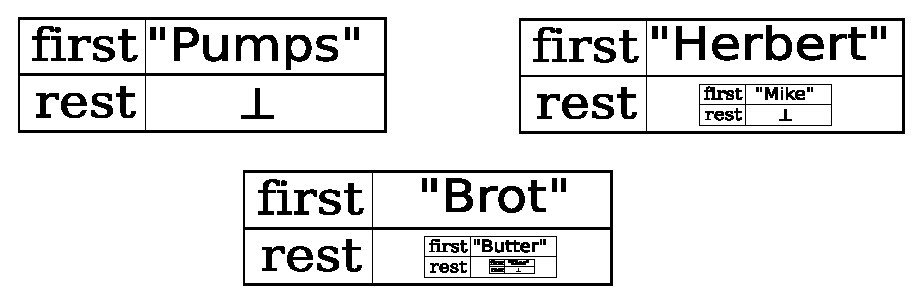
\includegraphics[width=0.8\textwidth]{i1list/pair-lists1}
  \caption{Liste mit Consen repräsentiert}
  \label{fig:cons-lists-1}
\end{figure}
Diesmal sind drei Conse im Spiel.  Die Liste wird jeweils
"<terminiert"> durch die leere Liste.  Abbildung~\ref{fig:cons-lists-1}
zeigt, wie die Listen aussehen, wenn sie wie andere zusammengesetzte
Daten als Tabellen dargestellt sind~-- das $\bot$ steht für die leere
Liste. Das sieht aus wie ineinandergeschachtelte russische Puppen und
entspricht damit nicht der gängigen Intuition, wie Listen aufgebaut
sind, aber es funktioniert.  Für viel mehr als drei Elemente
funktioniert die Darstellungsweise allerdings nicht: Darum bevorzugen
wir ab hier sogenannte "<Zeigerdiagramme">, bei denen alle Conse gleich groß
dargestellt sind und ein Pfeil zeigt, dass ein Cons die
\texttt{rest}-Komponente eines anderen Conses bildet.
Abbildung~\ref{fig:cons-lists-2} zeigt das Pfeildiagramm, das
Abbildung~\ref{fig:cons-lists-1} entspricht; es passt besser zur
gängigen Intuition von Listen.

\begin{figure}[tb]
  \centering
  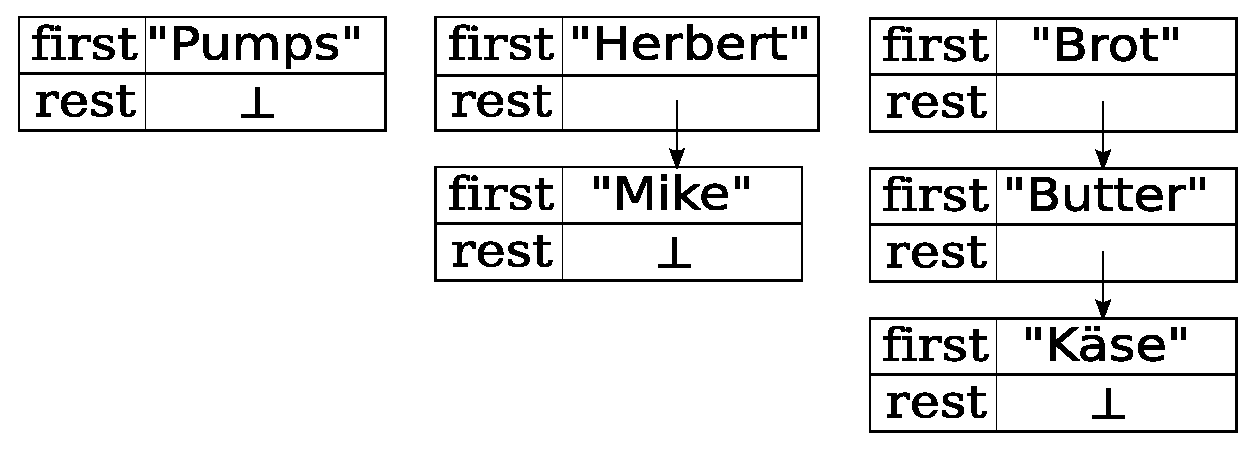
\includegraphics[width=0.8\textwidth]{i1list/pair-lists2}
  \caption{Liste mit Consen repräsentiert, als Pfeildiagramm}
  \label{fig:cons-lists-2}
\end{figure}


\section{Mit Listen programmieren}

Als erstes Beispiel für das Programmieren mit Listen schreiben wir
eine Funktion, die eine Liste von Zahlen akzeptiert und deren Summe
liefert.  Dazu werden erst einmal einige Beispiele solcher Listen
benötigt:
%
\begin{verbatim}
; Liste mit den Zahlen 1 2 3
(define n1 (cons 1 (cons 2 (cons 3 empty))))
; Liste mit den Zahlen e und pi
(define n2 (cons 2.7183 (cons 3.14159 empty)))
; Liste mit den Zahlen 2 3 5 7
(define n3 (cons 2 (cons 3 (cons 5 (cons 7 empty)))))
\end{verbatim}

Hier Kurzbeschreibung und Vertrag:\label{sec:list-sum}\index{list-sum@\texttt{list-sum}}
%
\begin{verbatim}
; Summe der Elemente einer Liste von Zahlen berechnen
(: list-sum (list-of-numbers -> number))
\end{verbatim}
%
Für die Testfälle halten die Beispiellisten her:
%
\begin{verbatim}
(check-expect (list-sum n1) 6)
(check-within (list-sum n2) 5.85989 0.001)
(check-expect (list-sum n3) 17)
\end{verbatim}
%
Nicht vergessen: In \texttt{n2} sind Zahlen mit Dezimalpunkt.
Deshalb müssen wir \texttt{check-within} verwenden.  Diese Funktion
hat drei Parameter: Die ersten beiden geben ein reales und ein
erwartetes Ergebnis an
und der dritte sagt, um wieviel das reale Ergebnis in der positiven
oder negativen Richtung vom erwarteten Ergebnis abweichen darf. Das Gerüst der
Funktion sieht so aus:
%
\begin{verbatim}
(define list-sum
  (lambda (lis)
    ...))
\end{verbatim}
%
(Es empfiehlt sich, als Bezeichner für Listen nicht einfach nur ein
\texttt{l} zu verwenden, da es in vielen Schriftarten der Ziffer
\texttt{1} ähnlich sieht.)

Zur Erinnerung: Listen sind zunächst gemischte Daten~-- die Definition
von \texttt{list-of-numbers} benutzt \texttt{mixed} mit zwei Fällen.  Entsprechend kommt die
Konstruktionsanleitung für gemischte Daten zur Anwendung:
%
\begin{verbatim}
(define list-sum
  (lambda (lis)
    (cond
      (... ...)
      (... ...))))
\end{verbatim}
%
Als nächstes sollten wir die Tests ergänzen, die auf die leere
Liste bzw.\ Conse testen.  % Für \texttt{empty} hat dieses Buch Dir
% den Test bisher vorenthalten: Das eingebaute Prädikat
% \texttt{empty?}\index{empty?@\texttt{empty?}} liefert \verb|#t| für
% die leere Liste und \verb|#f| für jeden anderen Wert.  Für Conse ist
% das Prädikat \texttt{cons?} bereits von der Record-Definition
% definiert:   %% HK das stand alles schon oben
%
\begin{verbatim}
(define list-sum
  (lambda (lis)
    (cond
      ((empty? lis) ...)
      ((cons? lis) ...))))
\end{verbatim}
%
Beim zweiten Zweig des \texttt{cond} handelt es sich um
zusammengesetzte Daten. Ergo ergänzen wir entsprechend der
Konstruktionsanleitung für zusammengesetzte Daten Selektor-Aufrufe in
die Schablone:
%
\begin{verbatim}
(define list-sum
  (lambda (lis)
    (cond
      ((empty? lis) ...)
      ((cons? lis)
       ... (first lis) ... (rest lis) ...))))
\end{verbatim}
%
Jetzt können wir ans Ausfüllen der beiden Zweige gehen: Die erste
Ellipse muss die Frage beantworten, was die Summe der leeren Liste sein
soll.  Diese Frage ist bei nahezu \emph{allen} Funktionen relevant,
die Listen akzeptieren, es empfiehlt sich darum grundsätzlich, einen
Testfall für die leere Liste zu formulieren:
%
\begin{alltt}
(check-expect (list-sum empty) \textrm{?})
\end{alltt}
%
Die Antwort ist nicht ganz offensichtlich, wir können 
sie aber durch folgende Überlegung gewinnen: Betrachten wir Listen aus
Einsen, dann entspricht deren Summe immer der Länge der Liste.  Wenn
die Liste leer ist hat sie die Länge $0$, entsprechend ist also auch
ihre Summe $0$:
%
\begin{alltt}
(check-expect (list-sum empty) 0)
\ldots
(define list-sum
  (lambda (lis)
    (cond
      ((empty? lis) 0)
      ((cons? lis)
       ... (first lis) ... (rest lis) ...))))
\end{alltt}
%
Bleibt der zweite Zweig mit den Consen.  Hier hilft es, die beiden
Selektor-Aufrufe \texttt{(first lis)} und \texttt{(rest lis)} auf die
Daten zurückzubeziehen.  \texttt{(first lis)} liefert für die drei
Beispiellisten folgende Werte:
%
\begin{alltt}
(first n1)
\evalsto{} 1
(first n2)
\evalsto{} 2.7183
(first n3)
\evalsto{} 2
\end{alltt}
%
Das ist jeweils das \emph{erste Element}~-- kein Wunder, dass der
Selektor \texttt{first}\index{first@\texttt{first}} heißt.  Nun für \texttt{rest}\index{rest@\texttt{rest}}:
%
\begin{alltt}
(rest n1)
\evalsto{} #<record:cons 2 #<record:cons 3 #<empty-list>>>
(rest n2)
\evalsto{}  #<record:cons 3.14159 #<empty-list>>
(rest n3)
\evalsto{} #<record:cons 3 #<record:cons 5 #<record:cons 7 #<empty-list>>>>
\end{alltt}
%
Dies sind jeweils Listen mit allen Elementen \emph{außer dem
  ersten}, also quasi den \emph{Rest}~-- daher der Name \texttt{rest}
für den Selektor.

Zurück zur Schablone: Was können wir mit dem ersten Element der Liste
und dem Rest der Liste anfangen?  Hier kommt ein besonderer Trick zum
Zug~-- da der Rest der Liste wieder eine Liste ist, können
wir von der Summe des Rests sprechen.  Wenn diese Summe bekannt
ist~-- also \emph{die Summe aller Elemente außer des ersten}, dann
könnten wir (und das Programm auch) die Gesamtsumme ermitteln, indem wir
auf diese Summe das noch fehlende erste Element addieren.  "<Die Summe
aller Elemente außer des ersten"> können wir so aufschreiben:
%
\begin{alltt}
(list-sum (rest lis))
\end{alltt}
%
Entsprechend die Summe des ersten Elements und der Summe des Rests:
%
\begin{alltt}
(+ (first lis) (list-sum (rest lis)))
\end{alltt}
%
Das können wir in die Schablone von oben einsetzen:
%
\begin{verbatim}
(define list-sum
  (lambda (lis)
    (cond
      ((empty? lis) 0)
      ((cons? lis)
       (+ (first lis) (list-sum (rest lis)))))))
\end{verbatim}
%
Dieses Programm ist nicht nur vollständig, es funktioniert auch
tatsächlich: Alles was wir gemacht haben war, die Kurzbeschreibung
von \texttt{list-sum} ernst zu nehmen, die behauptet, dass die Funktion
die Summe einer beliebigen Liste berechnet: \texttt{(rest lis)} ist
eine Liste, also kann \texttt{list-sum} auch deren Summe berechnen.

Um den "<Selbstaufruf"> von \texttt{list-sum} noch besser zu
verstehen, betrachten wir noch einmal die Datendefinition für
Listen zusammen mit der Datendefinition für Conse:

\begin{alltt}
; Eine \textbf{Liste} ist eins der folgenden:
; - die leere Liste
; - ein Cons
; Ein Cons besteht aus:
; - einem beliebigen Element
; - einer \textbf{Liste}
\end{alltt}
%
Die Datendefinition enthält einen Verweis auf \emph{sich selbst},
genannt \emph{Selbstbezug}\index{Selbstbezug}.  Dieser Selbstbezug ist
beim Rest~-- der Selbstaufruf, der in \texttt{list-sum} auf den Rest
erfolgt, folgt also der Datendefinition.  Ein Selbstaufruf
heißt auch \textit{rekursiver Aufruf}\index{rekursiver Aufruf} und ist
damit fester Bestandteil der Schablone für Funktionen, die Listen
akzeptieren:
%
\begin{alltt}
(: \textit{func} (list-of-numbers -> ...))

(define \textit{func}
  (lambda (lis)
    (cond
      ((empty? lis) ...)
      ((cons? lis)
       ... (first lis)
       ... (\textit{func} (rest lis)) ...))))
\end{alltt}
%
Jetzt wo wir die Schablone haben, gehen wir noch ein weiteres Beispiel
durch, bei dem wir sie von vornherein anwenden:  Gefragt ist eine
Funktion, die eine Liste von Zahlen akzeptiert und feststellt, ob alle
Listenelemente  positiv sind.  Die Funktion beantwortet eine
Ja/Nein-Frage, die damit auch die Kurzbeschreibung bildet:
%
\begin{alltt}
; sind alle Zahlen aus einer Liste positiv?
\end{alltt}
%
Hier ist der dazu passende Vertrag:\index{all-positive?@\texttt{all-positive?}}
%
\begin{verbatim}
(: all-positive? (list-of-numbers -> boolean))
\end{verbatim}
%
Für Testfälle stehen die leere Liste sowie die drei Beispiellisten
\texttt{n1}, \texttt{n2} und \texttt{n3} aus dem vorherigen Beispiel
zur Verfügung:
%
\begin{verbatim}
(check-expect (all-positive? empty) #t)
(check-expect (all-positive? n1) #t)
(check-expect (all-positive? n2) #t)
(check-expect (all-positive? n3) #t)
\end{verbatim}
%
Der \texttt{empty}-Testfall ist vielleicht etwas verwirrend: In der
Tat sind alle Elemente der leeren Liste positiv.  Eine andere Art dies
zu sagen wäre, dass kein Element der leeren Liste nicht positiv ist.

Diese Testfälle reichen sichtlich nicht aus, da alle \verb|#t| ergeben
sollen: Diese würden auch von folgender Funktion erfüllt:
%
\begin{verbatim}
(define all-positive?
  (lambda (lis)
    #t))
\end{verbatim}
%
Also werden noch Beispiele mit nicht-positiven Elementen benötigt~--
insbesondere eins mit dem Grenzfall $0$:
\begin{verbatim}
(check-expect (all-positive? (cons -5 empty)) #f)
(check-expect (all-positive? (cons 0 empty)) #f)
(check-expect (all-positive? (cons 1 (cons -2 empty))) #f)
\end{verbatim}
%
Das Gerüst ist wie folgt:
%
\begin{verbatim}
(define all-positive?
  (lambda (lis)
    ...))
\end{verbatim}
%
Wir können nun die Schablone für Listen direkt benutzen:
%
\begin{verbatim}
(define all-positive?
  (lambda (lis)
    (cond
      ((empty? lis) ...)
      ((cons? lis)
       ... (first lis)
       ... (all-positive? (rest lis)) ...))))
\end{verbatim}
%
Das Ergebnis im ersten Zweig wird durch den ersten Testfall diktiert:
\verb|#t|.  Wie schon zuvor machen wir uns die Bedeutung der
Ausdrücke im \texttt{cons}-Zweig klar:
\texttt{(first lis)} ist das erste Element der Liste.
\texttt{(all-positive? (rest lis))} besagt, ob alle Elemente
des Rests von \texttt{lis} positiv sind.  Es sind nur dann alle
Elemente von \texttt{lis} positiv, wenn \texttt{(first lis)}
positiv ist \emph{und} \texttt{(all-positive? (rest lis))} als Ergebnis
\verb|#t| liefert.  Damit ist klar, wie die beiden Ausdrücke
kombiniert werden müssen:
%
\begin{verbatim}
(define all-positive?
  (lambda (lis)
    (cond
      ((empty? lis) #t)
      ((cons? lis)
       (and (> (first lis) 0)
            (all-positive? (rest lis)))))))
\end{verbatim}
%
FIXME: Konstruktionsanleitung~\ref{ka:listen} auf Seite~\pageref{ka:listen}
fasst die Schablone für Funktionen, die Listen akzeptieren, noch einmal
zusammen. %%Die fehlt noch hier!

\section{Signaturkonstruktoren}

Die Beispiellisten vom Anfang dieses Kapitels sind allesamt
\textit{homogen}\index{homogen}: Alle Elemente der Liste sind jeweils
von derselben Sorte.  Es gibt eine Liste von Essenszutaten, eine von
Eigennamen, eine von Zahlen, eine von dramatischen Figuren, eine von
Frisuren und eine von Schuhen.  Die Datendefinition für
\texttt{list-of-numbers} von Seite~\ref{def:list-of-numbers} ist da allerdings nicht
festgelegt: es heißt ausdrücklich, dass jedes Cons ein
\emph{beliebiges} Element enthält.  So ist beispielsweise auch
folgende Liste zulässig:
%
\begin{verbatim}
(: ml1 list-of-numbers)
(define ml1 (cons 5 (cons "Herbert" empty)))
\end{verbatim}
%
In den meisten Fällen gehören jedoch alle Elemente einer Liste zu
derselben Sorte beziehungsweise haben dieselbe Signatur: Schön wäre
es, wenn die Signatur für die Liste dokumentieren könnte, welche
Signatur die Elemente haben.  Wir könnten bei
der Definition von \texttt{cons} die Signatur der Elemente angeben,
also \texttt{cons} zum Beispiel auf Elemente der Signatur
\texttt{number} fest abonnieren: 
%
\begin{alltt}
(define-record-functions cons-list
  cons
  cons?
  (first number)
  (rest  list-of-numbers))
(: cons (number list-of-\textbf{numbers} -> cons))
(: cons? (any -> boolean))
(: first (cons -> \textbf{number}))
(: rest (cons -> list-of-\textbf{numbers}))
\end{alltt}
%
Entsprechend würden wir die daraus resultierende Signatur für Listen
nicht mehr \texttt{list-of-numbers} sondern \texttt{list-of-numbers} nennen:\index{list-of-numbers@\texttt{list-of-numbers}}
%
\begin{verbatim}
(define list-of-numbers
  (signature
   (mixed empty-list
          cons-list)))
\end{verbatim}
%

FIXME

Mit
\texttt{define-record-functions} können wir die
Record-Definition von \texttt{cons} erweitern:
%
\begin{verbatim}
(define-record-functions (cons-of a)
  cons cons?
  (first a)
  (rest (list-of a)))
\end{verbatim}
%
\texttt{Cons-of} ist der Signaturkonstruktor.  (Das angehängte
\texttt{-of} ist, ähnlich wie das \texttt{make-} bei den
Konstruktoren, das \texttt{?} beim Prädikat und den Feld-Namen bei den
Selektoren reine Konvention.)

Konstruktor, Prädikat
und Selektoren für das neue \texttt{cons} haben die folgenden
Signaturen:
%
\begin{verbatim}
(: cons (%a (list-of %a) -> (cons-of %a)))
(: cons? (any -> boolean))
(: first ((cons-of %a) -> %a))
(: rest ((cons-of %a) -> (list-of %a)))
\end{verbatim}
%
Hier ist  \verb|%a| eine
\textit{Signaturvariable}, die für eine beliebige
Signatur steht, die erst beim Aufruf von \texttt{cons} beziehungsweise
\texttt{first} oder \texttt{rest} festgelegt wird.
Die Tatsache, dass hier zwei verschiedene Signaturvariablen
verwendet wurden bringt die zusätzliche Information für den
menschlichen Leser zum Ausdruck, dass die
Argumente von \texttt{cons-of} zu potentiell
unterschiedlichen Signaturen gehören.

Zu lesen sind die obigen Signaturdeklarationen so:
%
\begin{itemize}
\item \texttt{cons} akzeptiert zwei Argumente beliebiger Signaturen
  \verb|%a| und \verb|%b| und
  liefert als Resultat einen Record, dessen erstes Feld von der Signatur
  \verb|%a| und dessen zweites Feld von der Signatur \verb|%b| ist.
\item Das Resultat von \texttt{first} hat die
  Signatur des ersten Feldes seines Arguments.
\item Das Resultat von \texttt{rest} hat die
  Signatur des zweiten Feldes seines Arguments.
\end{itemize}
%

Diese Signaturen sind allerdings noch unbefriedigend, da sie nicht zum
Ausdruck bringen, dass das zweite Argument von \texttt{cons} immer
eine \emph{Liste} sein muss beziehungsweise dass \texttt{rest} immer
eine Liste liefert.  Diese Problematik stellen wir noch einen Moment
hintenan, werden aber später zu ihr zurückkehren~-- zunächst einmal zu
den Signaturen für Listen.

FIXME

Mit Hilfe von \texttt{cons-of} können wir versuchen, einen Ersatz für
\texttt{list-of-numbers} zu definieren, der spezifiziert, auf welche Signatur
die Elemente der Liste passen.  Das könnte so aussehen:
%
\begin{alltt}
(define list-of-numbers
  (signature
    (mixed empty-list
           (cons-of \textbf{number} list-of-numbers))))
\end{alltt}
%
Entsprechend für Zeichenketten:
%
\begin{alltt}
(define list-of-strings
  (signature
    (mixed empty-list
           (cons-of \textbf{string} list-of-strings))))
\end{alltt}
%
Wie schon oben angemerkt, wäre es unbefriedigend, für jede Elementsignatur eine
eigene Listensignatur definieren zu müssen, immer auf die gleiche
Weise.  Aber glücklicherweise unterscheiden sich
\texttt{list-of-numbers} und \texttt{list-of-strings} nur an einer
einzigen Stelle, und über die können wir abstrahieren:
%
\begin{verbatim}
(define list-of
  (lambda (x)
    (signature
      (mixed empty-list
             (cons-of x)))))
\end{verbatim}
%
Fertig!  Nun können wir Signaturen für Listen von Zahlen als
\texttt{(list-of number)}, Listen von Zeichenketten als
\texttt{(list-of string)} und Listen von beliebigen Werten als
\texttt{(list-of any)} schreiben.  Außerdem können wir diese
Definition jetzt verwenden, um bessere Signaturen für
\texttt{cons}, \texttt{first} und \texttt{rest} anzugeben:
%
\begin{verbatim}
(: cons (%a (list-of %a) -> (cons-of %a)))
(: cons? (any -> boolean))
(: first ((cons-of %a) -> %a))
(: rest ((cons-of %a) -> (list-of %a)))
\end{verbatim}
%

\section{Eingebaute Listen}

Da Listen in diesem Buch noch oft vorkommen und es umständlich
ist, jedesmal die Definitionen für \texttt{cons} und \texttt{list-of} an den Anfang
von Programmen zu setzen, ist es an dieser Stelle Zeit, eine neue
Sprachebene in \drscheme{} auszuwählen, nämlich \texttt{Schreibe Dein Programm!}
(ohne \texttt{Anfänger}).\index{Sprachebene}  Diese enthält \texttt{cons},
\texttt{cons?}, \texttt{first} und \texttt{rest} als eingebaute
Funktionen sowie den Signaturkonstruktor \texttt{list-of}\footnote{In Standard-Scheme heißt der Konstruktor für
  die eingebauten Conse \texttt{cons\index{cons@\texttt{cons}}}, die
  Selektoren \texttt{car\index{car@\texttt{car}}} und \texttt{cdr\index{cdr@\texttt{cdr}}}
  (gesprochen "<kar"> und "<kudder">; dies waren die Namen von Anweisungen auf einer
  Maschine, auf der ein Vorläufer von Scheme lief) und das Prädikat
  für die leere Liste \texttt{null?\index{null?@\texttt{null?}}}.} und eine
eingebaute Funktion \texttt{list} zur Erzeugung beliebiger Listen.

Außerdem werden nichtleere Listen ab dieser Sprachebene in der REPL
anders ausgedruckt, nämlich, der besseren Übersicht halber, als
\verb|#<list ...>|,
wobei die Listenelemente zwischen den spitzen Klammern aufgereiht sind.
Beispiele:

\begin{alltt}
(list 1)
\evalsto{} #<list 1>
(list 1 2)
\evalsto{} #<list 1 2>
(list 1 2 3)
\evalsto{} #<list 1 2 3>
\end{alltt}
%
\begin{feature}{\texttt{list}}{scheme:list}
  Die eingebaute Funktion \texttt{list}\index{list@\texttt{list}} erlaubt es, Listen aus ihren Elementen
  ohne Verwendung von \texttt{cons} zu erzeugen.  Sie
  akzeptiert eine beliebige Anzahl von Argumenten, macht daraus eine
  Liste und gibt diese zurück:
%
\begin{alltt}
(list 1 2 3)
\evalsto{} #<list 1 2 3>
(list "Axl" "Slash" "Izzy")
\evalsto{} #<list "Axl" "Slash" "Izzy">
\end{alltt}
\end{feature}


\section{Parametrische Polymorphie}
\label{sec:parametric-polymorphism}
\label{sec:more-lists}

In diesem Abschnitt programmieren wir eine Funktion, welche die Länge
einer Liste ermittelt.\index{list-length@\texttt{list-length}} Das ist
eine einfache Fingerübung mit einer interessanten Eigenschaft.  Hier
sind Kurzbeschreibung und Signatur:
%
\begin{alltt}
; Länge einer Liste berechnen
(: list-length ((list-of %a) -> natural))
\end{alltt}
%
FIXME:

Dieser Funktion ist egal, welche Signatur
die Elemente der Liste erfüllen, weil das Konzept der Länge einer
Liste unabhängig davon ist, was die Elemente sind.
Dementsprechend steht dort nur die Signaturvariable \verb|%a|.
Solche Funktionen, die Argumente akzeptieren, deren Signaturen
Signaturvariablen enthalten, heißen \textit{polymorph} oder auch
\textit{parametrisch polymorph} (weil die Signaturvariable eine Art
Parameter abgibt), und das dazugehörige Konzept heißt
\textit{parametrische
  Polymorphie}\index{Polymorphie}\index{parametrische Polymorphie}:
ein großes Wort, das hier für eine kleine Sache steht.  Interessantere
Beispiele für parametrische Polymorphie wird es in
Kapitel~\ref{cha:higher-order} geben.

Weiter mit \texttt{list-length}~-- hier ist das Gerüst:
%
\begin{alltt}
(define list-length
  (lambda (lis)
    ...))
\end{alltt}
%
Die Schablone ist wie gehabt:
%
\begin{alltt}
(define list-length
  (lambda (lis)
    (cond
      ((empty? lis) ...)
      ((cons? lis) 
       ... (first lis) ...
       ... (list-length (rest lis)) ...))))
\end{alltt}
%
Es ist \texttt{list-length} egal, was der Wert von \texttt{(first
  lis)} ist.  Die Länge der Liste ist unabhängig davon, was für Werte
sich darin befinden: entscheidend ist nur, wieviele es sind.  (Dieser
Umstand ist gerade verantwortlich für die parametrische Polymorphie.)
Damit können wir \texttt{(first lis)} aus der Schablone streichen und
diese dann zum vollständigen Rumpf ergänzen:
%
\begin{alltt}
(define list-length
  (lambda (lis)
    (cond
      ((empty? lis) 0)
      ((cons? lis) 
       (+ 1 
          (list-length (rest lis)))))))
\end{alltt}
%

\section{Funktionen, die Listen produzieren}

In den vorherigen Abschnitten haben wir ausschließlich Funktionen
programmiert, die Listen \emph{akzeptieren}.  In diesem Abschnitt
schreiben wir Funktionen, die Listen \emph{produzieren}.  Das geht mit
Techniken, die wir bereits vorgestellt haben.  Wir machen die Sache
interessanter, indem wir in einem ersten Beispiel Listen von
zusammengesetzten Daten betrachten und in einem zweiten Beispiel zwei
Listen verarbeiten.

\subsection{Gürteltiere überfahren}

Auf Seite~\pageref{page:run-over-dillo} haben wir die Funktion
\texttt{run-over-dillo} geschrieben, die für das Überfahren von
Gürteltieren zuständig ist.  In diesem Abschnitt schreiben wir die
Funktion, die das gleich massenweise erledigt, beispielsweise für alle
Gürteltiere auf einem Highway.  Dazu übernehmen wir Daten- und
Record-Definition von Gürteltieren aus
Abschnitt~\ref{page:run-over-dillo} sowie die Funktiondefinition von
\texttt{run-over-dillo}.  Gürteltiere können wir in Listen stecken,
ebenso wie Zahlen, Zeichenketten oder boolesche Werte.  Hier ist ein
Beispiel:
%
\begin{verbatim}
; Gürteltiere auf Highway 75
(define dl75 (list d1 d2 d3 d4))
\end{verbatim}
(\texttt{D1}, \texttt{d2}, \texttt{d3} und \texttt{d4} sind die
Beispielgürteltiere aus Abschnitt~\ref{page:run-over-dillo}.)

Diese Liste hat die Signatur \texttt{(list-of dillo)}.  Wenn wir eine
Funktion schreiben wollen, die alle Gürteltiere aus einer Liste
überfährt, müsste diese also folgende Kurzbeschreibung und Signatur
haben:
%
\begin{verbatim}
; Gürteltiere überfahren
(: run-over-dillos ((list-of dillo) -> (list-of dillo)))
\end{verbatim}
%
Als Testfall kann obige Beispielliste herhalten:
%
\begin{verbatim}
(check-expect (run-over-dillos dl75)
              (list (make-dillo 55000 #f)
                    d2
                    (make-dillo 60000 #f)
                    d4))
\end{verbatim}
%
Zur Erinnerung: \texttt{d2} und \texttt{d4} sind bereits tot,
dementsprechend sind sie überfahren wie zuvor.

Hier ist das Gerüst:
%
\begin{verbatim}
(define run-over-dillos
  (lambda (dls)
    ...))
\end{verbatim}
%
Die Funktion akzeptiert eine Liste als Eingabe, wir können also, wie
schon so oft, die entsprechende Schablone zum Einsatz bringen:
%
\begin{verbatim}
(define run-over-dillos
  (lambda (dls)
    (cond
     ((empty? dls) ...)
     ((cons? dls)
      ... (first dls) ...
      ... (run-over-dillos (rest dls)) ...))))
\end{verbatim}
%
Im ersten Zweig ist die Sache klar: Geht eine leere Liste rein, kommt
auch eine leere Liste raus.  Im zweiten Zweig können wir uns erst
einmal um das erste Gürteltier kümmern.  Wir haben ja bereits eine
Funktion, die ein einzelnes Gürteltier überfährt; diese können wir auf
das erste Element der Liste anwenden:
%
\begin{verbatim}
(define run-over-dillos
  (lambda (dls)
    (cond
     ((empty? dls) empty)
     ((cons? dls)
      ... (run-over-dillo (first dls)) ...
      ... (run-over-dillos (rest dls)) ...))))
\end{verbatim}
%
Lesen wir noch einmal die beiden Ausdrücke, die im zweiten Zweig
stehen:
%
\begin{itemize}
\item \texttt{(run-over-dillo (first dls))} ist das erste Gürteltier
  der Liste, überfahren.
\item \texttt{(run-over-dillos (rest dls))} ist eine Liste der
  restlichen Gürteltiere, überfahren.
\end{itemize}
%
Gefragt ist eine Liste \emph{aller} Gürteltiere, überfahren:
Wir müssen also nur die Resultate der beiden Ausdrucke mit
\texttt{cons} kombinieren:
%
\begin{verbatim}
(define run-over-dillos
  (lambda (dls)
    (cond
     ((empty? dls) empty)
     ((cons? dls)
      (cons (run-over-dillo (first dls))
                 (run-over-dillos (rest dls)))))))
\end{verbatim}
%
Fertig!

Dieses Beispiel zeigt, dass wir für Funktionen, die Listen produzieren,
keine neue Technik brauchen: Wenn eine Funktion eine leere Liste
produzieren soll, benutzen wir an der entsprechenden Stelle
\texttt{empty}, und bei nichtleeren Listen benutzen wir
\texttt{cons}, bringen also die Schablone für Funktionen zum
Einsatz, die zusammengesetzte Daten produzieren.

\subsection{Zwei Listen aneinanderhängen}
In unserem nächsten Beispiel ist eine Funktion
\texttt{concatenate}\index{concatenate@\texttt{concatenate}} gefragt, die zwei
Listen aneinanderhängt:\label{sec:concatenate}
% 
\begin{alltt}
(concatenate (list 1 2 3) (list 4 5 6))
\evalsto{} #<list 1 2 3 4 5 6>
\end{alltt}
%
Kurzbeschreibung, Signatur und Gerüst sehen folgendermaßen aus:\index{concatenate@\texttt{concatenate}}
%
\begin{alltt}
; zwei Listen aneinanderhängen
(: concatenate ((list-of %a) (list-of %a) -> (list-of %a)))
(define concatenate
  (lambda (lis-1 lis-2)
    ...))
\end{alltt}
%
Die Konstruktionsanleitung aus Abschnitt~\ref{sec:lists} ist
eigentlich nur für Funktionen gedacht, die eine einzelne Liste
akzeptieren.  Welche von beiden ist das $l$ aus der Anleitung?  Im
Zweifelsfall können wir beide Alternativen ausprobieren.  Wir
fangen, um die Sache spannender zu machen, mit \texttt{lis-2} an:
%
\begin{alltt}
(define concatenate
  (lambda (lis-1 lis-2)
    (cond
      ((empty? lis-2) ...)
      ((cons? lis-2) 
       ... (first lis-2)
       ... (concatenate lis-1 (rest lis-2)) ...))))
\end{alltt}
%
Der erste Zweig des \texttt{cond} ist noch einfach: Wenn
\texttt{lis-2} leer ist, muss \texttt{lis-1} herauskommen.  Jedoch wäre für
das obige Beispiel der Wert von \texttt{(concatenate lis-1 (rest lis-2))} die
folgende Liste:
%
\begin{alltt}
#<list 1 2 3 5 6>
\end{alltt}
%
Bei dieser Liste fehlt das
Element 4 in der Mitte, und es ist nicht ersichtlich, wie unsere Funktion
sie passend ergänzen könnte.  Diese
Möglichkeit führt also in eine Sackgasse. Wir versuchen deshalb, die Schablone  auf
\texttt{lis-1} 
 statt auf \texttt{lis-2} anzuwenden:
%
\begin{alltt}
(define concatenate
  (lambda (lis-1 lis-2)
    (cond
      ((empty? lis-1) ...)
      ((cons? lis-1) 
       ... (first lis-1)
       ... (concatenate (rest lis-1) lis-2) ...))))
\end{alltt}
%
Die erste Ellipse ist einfach zu ersetzen:  Ist die erste Liste
leer, ist das Ergebnis die zweite Liste \texttt{lis-2}.  Für den
zweiten Fall sollten wir uns noch einmal ins Gedächtnis rufen,
was für einen Wert \texttt{(concatenate (rest lis-1) lis-2)} liefert: das Ergebnis
dieses Aufrufs ist eine
Liste, die aus \texttt{(rest lis-1)} und \texttt{lis-2} zusammengesetzt
wurde.  Auf das obige Beispiel übertragen, mit \texttt{lis-1} $=$
\verb|#<list 1 2 3>| und \texttt{lis-2} $=$
\verb|#<list 4 5 6>|, ist \texttt{(rest lis-1)} $=$ \verb|#<list 2 3>|.
Der Wert von \texttt{(concatenate (rest lis-1) lis-2)} wäre
also:
%
\begin{alltt}
#<list 2 3 4 5 6>
\end{alltt}
%
Es fehlt das erste Element von \texttt{lis-1}, \texttt{(first
  lis-1)}, das vorn an das Ergebnis angehängt werden muss.  Das geht
mit \texttt{cons}:
%
\begin{alltt}
(define concatenate
  (lambda (lis-1 lis-2)
    (cond
      ((empty? lis-1) lis-2)
      ((cons? lis-1) 
       (cons (first lis-1)
                  (concatenate (rest lis-1) lis-2))))))
\end{alltt}
%
Dieses Beispiel zeigt ein weiteres Schablonenelement, das noch öfter
vorkommen wird:  Wie bei anderen zusammengesetzten Daten müssen Funktionen, die
Listen konstruieren sollen, irgendwo ein \texttt{cons} enthalten.

\texttt{List-length} und \texttt{concatenate} sind gute
Programmierübungen.  Da viele Programme diese Operationen benötigen,
sind sie in den Lehrsprachen  bereits unter den Namen
\texttt{length}\index{length@\texttt{length}} und
\texttt{append}\index{append@\texttt{append}} eingebaut.


\section*{Anmerkungen}

Listen sind, was Datenstrukturen betrifft, eine Art Alleskleber:
Sie taugen auch für die Repräsentation von Tabellen,
Mengen und vielen anderen zusammengesetzten Daten.  Für Listen gibt es
eine riesige Anzahl praktischer Funktionen, von denen die Funktionen in
diesem Kapitel nur die Spitze des Eisberges sind.  Da 
ab hier Listen in den Lehrsprachen fest eingebaut sind, können sie als universelles
Kommunikationsmittel zwischen Programmen dienen, weil sich Funktionen
auf Listen aus einem Programm auch in einem anderen verwenden lassen.
Dies unterscheidet funktionale Sprachen von vielen anderen Programmiersprachen, in
denen Listen vom Programmierer selbst definiert werden müssen oder nur
eine untergeordnete Rolle spielen.

Viele andere Programmiersprachen bauen auf \textit{Felder\index{Feld}} oder
\textit{Arrays\index{Array}} als fundamentale Datenstrukturen für die
Repräsentation von Folgen.  Diese gibt es in
Scheme auch (unter dem Namen \textit{Vektor\index{Vektor}}), finden jedoch
nur selten Verwendung: Oft lässt sich eine
bessere Lösung mit Listen oder anderen Repräsentationen finden.

\section*{Aufgaben}

\begin{aufgabe}
  Schreibe Ausdrücke für Listen, welche die Beispiellisten vom
  Anfang von Abschnitt~\ref{sec:lists} repräsentieren.
\end{aufgabe}

\begin{aufgabe}
Schreibe folgende Funktionen auf Listen:
  
  \begin{enumerate} 
    
  \item Eine Funktion \texttt{count-zeroes}, die die Anzahl von Nullen
    in einer Liste von Zahlen berechnet.
    
  \item Eine Funktion \texttt{contains>10?}, die feststellt, ob eine
    Liste von Zahlen eine Zahl enthält, die größer als 10 ist.
    
  \item Eine Funktion \texttt{list-length}, die die Länge einer Liste
    von Zahlen berechnet.

  \end{enumerate}
  
\end{aufgabe}

\begin{aufgabe}
   Auf einem Acker gibt es ~--- vereinfacht
  dargestellt~--- Kartoffeln, Erdklumpen und Steine.  Ein
  Ackerbestandteil ist also eine Kartoffel, ein Erdklumpen oder ein
  Stein.  Jedes dieser Ackerbestandteile hat ein Gewicht in Gramm;
  Kartoffeln besitzen außerdem zusätzlich noch die Eigenschaft, ob sie
  essbar sind oder nicht (und daher aussortiert werden müssen).
  Schreibe ein Programm für eine Kartoffel-Erntemaschine, die die
  essbaren Kartoffeln aus den Ackerbestandteilen herausfiltern muss.

  \begin{enumerate}
  \item Führe eine Datenanalyse für
    Ackerbestandteile durch und schreibe passende Daten- und
    Recorddefinitionen.  Gib ein paar Beispiele für
    Ackerbestandteile an, die Du in den nächsten Teilaufgaben in
    Testfällen verwenden kannst.

  \item Schreibe eine Funktion
    \texttt{edible-potato?}, die überprüft ob ein übergebener
    Ackerbestandteil eine essbare Kartoffel ist.

  \item Schreibe eine Funktion \texttt{weight}, 
    die das Gewicht eines beliebigen Ackerbestandteils zurückgibt.

  \item Schreibe eine Daten- und Recorddefinition
    für Listen von Ackerbestandteilen.  Gib alle Signaturen an!
    Gib außerdem mindestens fünf verschiedene Beispiele für Listen
    mit Ackerbestandteilen an.

  \item Schreibe eine Funktion \texttt{total-weight},
    die eine Liste von Ackerbestandteilen akzeptiert und das Gesamtgewicht
    aller Ackerbestandteile in der Liste ausrechnet.

  \item Schreibe eine Funktion
    \texttt{total-edible-potatoes-weight}, die eine Liste von Ackerbestandteilen
    akzeptiert und das Gesamtgewicht aller essbaren Kartoffeln in der Liste
    ausrechnet.

  \item Schreibe eine Funktion \texttt{count}, die 
    eine Liste von Ackerbestandteilen akzeptiert und die Anzahl der
    Ackerbestandteile in der Liste bestimmt.

  \item Schreibe eine Funktion
    \texttt{count-edible-potatoes}, die eine Liste von
    Ackerbestandteilen akzeptiert und die Anzahl der essbaren
    Kartoffeln in der Liste bestimmt.

  \item Eine Maschine soll nun die Kartoffeln aus dem
    Acker automatisch ernten.  Leider ist die Maschine sehr alt und
    kommt deswegen mit großen Steinen und Erdklumpen nicht klar.  Der
    Erntevorgang wird abgebrochen, sobald ein Stein oder ein
    Erdklumpen, der schwerer als 1kg ist, in die Maschine gerät.
    Schreibe die Funktion \texttt{harvester}, die diesen Vorgang
    simuliert. Als Eingabe bekommt diese Funktion eine Liste von
    Ackerbestandteilen, die sie nach und nach abarbeitet.
    Herauskommen soll eine Liste von Ackerbestandteilen, in der die
    geerneteten essbaren Kartoffeln enthalten sind.  Schreibe
    ausreichend Testfälle, beachte auch den Fall, dass die
    Maschine im Leerlauf betrieben wird.  Verwende die Funktionen
    aus den vorherigen Aufgabenteilen.

  \item Schreibe eine Funktion
    \texttt{heaviest-potato}, die aus einer Liste von
    Ackerbestandteilen die schwerste essbare Kartoffel heraussucht und
    zurückgibt.  Wenn in der Liste keine essbare Kartoffel enthalten ist, soll
    die Funktion \verb|#f| zurückgeben.

    \item Schreibe eine Funktion
      \texttt{filter-edible-potatoes}, die eine Liste von
      Ackerbestandteilen akzeptiert und essbaren Kartoffeln als Liste
      zurückgibt.

    \item Schreibe eine Funktion
      \texttt{drop-stones}, die eine Liste von Ackerbestandteilen
      akzeptiert und eine Liste zurückgibt, in der es keine Steine mehr
      gibt.

    \item Schreibe eine Funktion
      \texttt{average-weight-edible-potatoes}, die eine Liste von
      Ackerbestandteilen akzeptiert und das durchschnittliche Gewicht
      der essbaren Kartoffeln berechnet.

  \end{enumerate}
  
\end{aufgabe}

\begin{aufgabe}
  Wir repräsentieren einen Lithium-Ionen-Akku als
  eine Liste von Lithium-Ionen-Zellen.  Eine Zelle besteht aus einer
  maximalen Ladung (in Milliamperestunden, mAh) und einer momentanen
  Ladung (ebenfalls in mAh).

  Wenn eine Zelle eine Ladung von 1000mAh hat, bedeutet das, dass die
  Zelle eine Stromstärke von 1000mA (Milliampere) für eine Stunde lang
  liefern kann.  Die momentane Ladung darf nie über die maximale
  Ladung steigen und nie unter 10\% der maximalen Ladung fallen, in
  unserer Beispielzelle also 100mAh, sonst geht die Zelle kaputt.

  % Die Zellen werden nach der Reihe ge- bzw.  entladen.  Wenn die erste
  % Zelle auf 400mAh entladen ist, wird die zweite Zelle entladen, dann
  % die nächste, etc.  Geladen wird in anderer Richtung: Zuerst wird die
  % letzte Zelle geladen, dann die davor, etc.
  
  \begin{enumerate}
    \setlength{\itemsep}{1cm}
  \item Führe eine Datenanalyse für Li-Ionen-Akkus und
    Li-Ionen-Zellen durch, schreibe die Datendefinitionen auf und
    setze die Datendefinitionen um.

  \item Schreibe folgende Funktionen:

    \begin{itemize}
    \item \texttt{cell-full?}, die überprüft, ob eine
      Zelle vollständig geladen ist (d.h. ob die momentante
      Ladung gleich der maximalen Ladung ist)

    \item \texttt{cell-empty?}, die überprüft, ob eine Zelle entladen
      ist (d.h. ob die momentane Ladung gleich der minimalen Ladung
      ist, also 10\% der maximalen Ladung)

    \item \texttt{cell-defect?}, die überprüft, ob eine
      Zelle defekt ist (d.h. ob die momentane Ladung die
      maximale Ladung überschreitet oder die minimale Ladung
      unterschreitet)

    \item \texttt{cell-ok?}, die überprüft, ob eine
      Zelle funktioniert (d.h. ob die momentane Ladung
      innerhalb der minimalen und maximalen Ladung liegt)

    \end{itemize}

  \item Schreibe folgende Funktionen:

    \begin{itemize}
    \item \texttt{battery-full?}, die überprüft, ob ein Akku
      vollständig geladen ist (d.h. ob alle Zellen voll sind); eine
      Batterie ohne Zelle gilt als geladen.

    \item \texttt{battery-empty?}, die überprüft, ob ein Akku entladen
      ist (d.h. ob alle Zellen leer sind); eine Batterie ohne Zelle
      gilt auch als leer.

    \item \texttt{battery-defect?}, die überprüft, ob ein Akku defekt
      ist (d.h. ob mindestens eine Zelle defekt ist); eine Batterie
      ohne Zelle gilt als nicht defekt.

    \item \texttt{battery-ok?}, die überprüft, ob ein Akku
      funktioniert (d.h. ob alle Zellen funktionieren); eine Batterie
      ohne Zelle gilt als funktionstüchtig.
      
    \end{itemize}

    \textbf{Gehe in den folgenden Teilaufgaben davon aus, dass
      nur \emph{funktionierende} Zellen und Batterien übergeben
      werden!}

  \item Das Ladegerät kann eine Zelle um 500mAh pro Stunde
    aufladen.  Schreibe eine Funktion \\
    \texttt{time-to-fully-charge-cell}, die ausrechnet, wieviele
    Stunden es dauert, bis das Ladegerät die Zelle aufgeladen hat.

  \item Schreibe eine Funktion
    \texttt{time-to-fully-charge-battery}, die ausrechnet, wieviele
    Stunden es dauert, bis das Ladegerät den Akku aufgeladen hat.

  \item Schreibe eine Funktion \texttt{charge-cell}, die eine
    Zelle und eine Zeit in Stunden konsumiert und die Zelle
    zurückgibt, die mit dem in der vorherigen Teilaufgabe genannten
    Ladegerät für die übergebene Zeit geladen wurde.  Die Ladung darf
    aber nicht über die maximale Ladung steigen!  Die restliche Zeit
    verfällt, wenn die Zelle bereits voll ist.

  \item Schreibe eine Funktion \texttt{charge-battery}, die einen
    Akku auflädt.  Die Funktion gibt einen Akku zurück, der mit dem
    Ladegerät für die übergebene Zeit geladen wurde.  Ist eine Zelle
    vollständig geladen, so wird die nächste Zelle mit der restlichen
    Zeit geladen.  Sind alle Zellen geladen und ist die Zeit jedoch
    noch nicht aufgebraucht, so verstreicht diese.

  \item Das Entladen einer Zelle hängt vom Verbraucher ab: Ein Gerät
    hat einen Verbrauchswert, angegeben in mA.  Anschaulich betrachtet
    heißt das, dass das Gerät pro Zeit eine gewissen Strom verbraucht.
    Schreibe eine Funktion \texttt{time-to-fully-discharge-cell},
    die eine Zelle und einen Verbrauch pro Stunde konsumiert und
    ausrechnet, wie lange es dauert, bis die Zelle entladen ist.

  \item Schreibe eine Funktion
    \texttt{time-to-fully-discharge-battery}, die einen Akku und einen
    Verbrauch pro Stunde konsumiert, und ausrechnet, wie lange es
    dauert, bis der Akku entladen ist.

  \item Schreibe eine Funktion \texttt{discharge-cell}, die eine
    Zelle, einen Verbrauch pro Stunde und die Dauer (in Stunden)
    konsumiert, für die der Verbraucher den Strom der Zelle
    verbraucht.  Die Funktion soll eine Zelle zurückgeben, die für die
    Dauer den Verbraucher mit Strom versorgt hat.  Die Ladung darf
    aber nicht unter die minimale Ladung fallen! Die restliche Zeit
    verfällt, wenn die Zelle bereits leer ist (tatsächlich geht dem
    Verbraucher einfach der Strom aus...).

  \item Schreibe eine Funktion \texttt{discharge-battery}, die
    eine Batterie, einen Verbrauch pro Stunde und die Dauer (in
    Stunden) konsumiert.  Die Funktion soll eine Batterie,
    zurückgeben, die für die Dauer den Verbraucher mit Strom versorgt
    hat.  Ist die Ladung einer Zelle verbraucht, wird die Ladung der
    nächsten Zelle für die verbleibende Zeit verbraucht.  Sind alle
    Zellen entladen und ist die Zeit jedoch noch nicht aufgebraucht,
    so verstreicht diese, dem Verbraucher geht der Strom aus.

  \end{enumerate}
  
\end{aufgabe}

\begin{aufgabe}
   Schreibe eine Funktion, die auf möglichst
  einfache Weise eine Liste von Zahlen aufsteigend sortiert! Gehe
  dazu wie folgt vor:

  FIXME: nichtleere Listen!
  
  \begin{enumerate}
  \item Schreibe eine Funktion
    \texttt{list-min}, die das kleinste Element einer
    Liste zurückgibt.

    Beispiel: \verb|(list-min (list 2 3 4 1 5 6))| ergibt \verb|1|

    Wenn die Funktion auf eine leere Liste angewendet
    wird, soll die Funktion eine \texttt{violation} produzieren.
  \item Schreibe eine Funktion
    \texttt{delete-once}, die aus einer Liste von Zahlen das erste
    Vorkommen einer gegebenen Zahl entfernt.

    Beispiel: \verb|(delete-once 5 (list 1 2 5 3 4 5))| ergibt
    \verb|#<list 1 2 3 4 5>|
    
    (Wenn die Liste die Zahl nicht enthält,
    soll sie unverändert zurückgegeben werden.)
  \item  Schreibe eine Funktion \texttt{sort}, die
    eine Liste von Zahlen in aufsteigender Reihenfolge sortiert.
    Benutze dazu \texttt{list-min} und \texttt{delete-once}.

    Beispiel: \verb|(sort (list 1 5 3 2 4))| ergibt
    \verb|#<list 1 2 3 4 5>|

  \end{enumerate}
\end{aufgabe}

\begin{aufgabe}
   In einer Firma stempeln die Mitarbeiter Stempelkarten, um ihre
  Arbeitszeit nachzuweisen: Auf jeder Stempelkarte ist die Nummer des
  Mitarbeiters vermerkt sowie eine Liste von jeweils gearbeiteten
  Stunden. Gehe der Einfachheit halber davon aus, dass nur ganze Stunden
  notiert werden.
  Außerdem gibt es für jeden Mitarbeiter eine Personalakte
  mit Name, Nummer und Stundenlohn (auch nur in ganzen Euros) des Mitarbeiters.
  Am Ende jedes Monats 
  muss an jeden Mitarbeiter der Lohn überwiesen werden.  Dazu werden
  Überweisungen erzeugt; jede Überweisung besteht aus der
  Mitarbeiternummer und einem Überweisungsbetrag.

  Schreibe Daten- und Record-Definitionen für Stempelkarten,
  Personalakten und Überweisungen.

  Schreibe eine Funktion, die eine Liste von Personalakten
  und eine Liste von Stempelkarten für einen Monat akzeptiert, für jeden
  Mitarbeiter die gearbeiteten Stunden aufsummiert und eine
  Liste der Überweisungen zurückliefert.
\end{aufgabe}

\begin{aufgabe}
   Du bist Besitzer eines Parkplatzes mit
  Bereichen für unterschiedliche Fahrzeuge:  PKWs (\texttt{car}), Lastwagen
  (\texttt{truck}), Wohnmobile (\texttt{caravan)}, Busse (\texttt{bus})
  und Fahrräder (\texttt{bike}). 
  Wegen der Finanznot hat die Stadt Tübingen beschlossen, dass 
  Du für jedes Fahrzeug, das auf Ihrem Parkplatz
  parkt, Abgaben entrichten musst, und zwar pro Tag je:
  \begin{list}{-}{}
  \item \texttt{car}: 3 Cent
  \item \texttt{truck}: 5 Cent + 3 Cent pro Achse
  \item \texttt{caravan}: 4 Cent
  \item \texttt{bus}: 10 Cent + 1 Cent pro Sitzplatz
  \item \texttt{bike}: 1 Cent.
  \end{list} 
  Der Fahrzeughalter kann die Abgaben nur für den jeweiligen Tag begleichen, 
  so dass Du die Parkdauer nicht beachten musst.

  \begin{enumerate}
  \item Mache eine Datenanalyse und schreibe Daten- und 
    Recorddefinitionen für die Fahrzeugtypen \texttt{truck}, \texttt{bus} und
    \texttt{simple-vehicle}. Dabei werden unter \texttt{simple-vehicle} die
    Fahrzeuge zusammengefasst, bei denen keine variablen Kosten anfallen.
  \item Schreibe  Funktionen
    \texttt{tax-truck}, \texttt{tax-bus} und \texttt{tax-simple-vehicle}
    zur Ermittlung der Abgaben für diese Fahrzeugtypen
  \item Definiere einen Datentyp \texttt{vehicle}. Schreibe eine
    Funktion \texttt{tax-vehicle}, die die Abgaben für ein beliebiges Fahrzeug 
    berechnet.    
  \item Schreibe nun eine Funktion \texttt{calculate-tax}, die die täglichen 
    Abgaben berechnet, die Du an das Finanzamt für alle Fahrzeuge auf ihrem Parkplatz
    bezahlen musst. Die Funktion akzeptiert eine Liste von Fahrzeugen und
    berechnet die Gesamtabgaben eines Tages.
  \end{enumerate}
  Benutze bei jeder Funktion und jedem Record, den Du schreibst,
  die Konstruktionsanleitungen: Erstelle zunächst
  Kurzbeschreibung, Signatur, einige Testfälle und das Gerüst der Funktion.
  Vervollständige anschließend das Gerüst und vergewissere Dich,
  dass die Testfälle korrekt durchlaufen!
\end{aufgabe}

\begin{aufgabe}
  Da Du jetzt mit Listen programmieren kannst, bittet Dr.~Knaubichler
  Dich nochmals um Ihre Hilfe (siehe Aufgabe~\ref{aufgabe:knaubichler2}
  aus dem vorigen Kapitel, Seite~\pageref{aufgabe:knaubichler2}):
  Schreibe ein Programm, das aus einer Liste von Grundkreaturen
  die zwei Grundkreaturen auswählt, die miteinander gekreuzt die
  leistungsstärkste Kreatur ergeben.

  Gehen dazu wie folgt vor:

  \begin{enumerate}
  \item Schreibe ein Prädikat für Kreaturen.

  \item Schreibe eine Funktion
    \texttt{creature-power}, die eine beliebige Kreatur akzeptiert und
    deren Leistung berechnet.  Die Leistung ist die Summe aller
    Eigenschaften.

  \item  Schreibe eine Funktion
    \texttt{find-optimal-breeding-partner}, die eine Grundkreatur
    $c_1$ und eine Liste von Grundkreaturen akzeptiert.  Die Funktion
    soll die Grundkreatur $c_2$ aus der Liste auswählen und
    zurückgeben, die der beste Kreuzungspartner von $c_1$ ist.  Die
    Kreuzung von $c_1$ und $c_2$ soll also unter allen möglichen
    Kreuzungen die Kreatur mit der höchsten Leistung ergeben.  Falls
    die Liste der Grundkreaturen leer ist, soll die Funktion \verb|#f|
    zurückgeben.

  \item  Schreibe eine Funktion
    \texttt{breed-optimal-partner}, die eine Grundkreatur $c_1$ und
    eine Liste von Grundkreaturen akzeptiert.  Die Funktion soll $c_1$
    mit der Grundkreatur aus der Liste kreuzen, die zur
    leistungsstärksten Kreatur führt.  Falls die Liste der
    Grundkreaturen leer ist, soll die Funktion \verb|#f| zurückgeben.
    Benutze \texttt{find-optimal-breeding-partner}.

  \item  Schreibe eine Funktion
    \texttt{optimal-breed}, die eine Liste von Grundkreaturen
    akzeptiert.  Die Funktion soll die beiden Grundkreaturen aus der
    Liste miteinander kreuzen, die unter allen möglichen Kreuzungen
    die Kreatur mit der höchsten Leistung ergeben.  Benutze die
    Funktionen aus den vorherigen Teilaufgaben.

  \end{enumerate}
\end{aufgabe}

%%% Local Variables: 
%%% mode: latex
%%% TeX-master: "i1"
%%% End: 


% Diese Datei ist Teil des Buchs "Schreibe Dein Programm!"
% Das Buch ist lizensiert unter der Creative-Commons-Lizenz
% "Namensnennung - Weitergabe unter gleichen Bedingungen 4.0 International (CC BY-SA 4.0)"
% https://creativecommons.org/licenses/by-sa/4.0/deed.de

\chapter{Exkurs: Induktive Beweise und Definitionen}
\label{cha:indu}

In den vergangenen Kapiteln haben wir uns oft mit Selbstbezügen in
Datendefinitionen beschäftigt und den rekursiven Funktionen, die sie
akzeptieren.  Dieses Kapitel beschäftigt sich mit der mathematischen
Seite solcher Funktionen.  Es ist für Dich als Lektüre sinnvoll, wenn
Du Dich besonders für Mathematik interessierst oder studiumshalber
dafür interessieren musst.  Für das Verständnis der folgenden Kapitel
kannst Du es aber auch weglassen.

Die Mathematik bildet Daten mit Selbstbezug als sogenannte
\textit{induktiv definierte} Mengen ab.  Dies ermöglicht uns, dass wir
uns von der Korrektheit einer Funktion mit Hilfe eines sogenannten
induktiven Beweises überzeugen.  Dieses Kapitel zeigt, was das ist und
wie das geht.

\section{Aussagen über natürliche Zahlen}
\label{sec:mathematical-induction}
\label{sec:gausssche-summenformel}

In der Mathematik gibt es viele kuriose Aussagen über natürliche
Zahlen.  Legendenstatus hat z.B.\ die Gaußsche
Summenformel\index{Gaußsche Summenformel}.  Diese besagt, dass für
eine natürliche Zahl $n$ die Summer aller Zahlen von 1 bis $n$ mit der
Formel
\[\frac{n\times (n+1)}{2}\]
berechnet werden kann: Man muss also gar nicht mühsam die Zahlen
einzeln addieren.  Mathematiker lieben spezielle Schreibweisen und
könnten Gauß' Behauptung folgendermaßen aufschreiben:
%
\[\forall n\in\mathbb{N}: \sum_{i=0}^n i =
  \frac{n\times (n+1)}{2}\]
%
Das $\forall$ heißt "<für alle">, das $\in$ heißt "<Element von">
$\mathbb{N}$ ist das Kürzel für die Menge der natürlichen Zahlen.
Am Anfang steht also "<für alle $n$, die Element von $\mathbb{N}$
sind"> oder ganz lapidar "<für alle natürlichen Zahlen $n$">.

Das $\sum$ ist ein griechisches Sigma und steht für "<Summe">.  Das
$i=0$ untendrunter und das $n$ obendrüber bedeuten, dass eine neue
Variable $i$ eingeführt wird, und die nacheinander die Werte $0, 1, 2,
\ldots n$ annimmt, und für jeden Wert in die Formel rechts vom $\sum$
eingesetzt wird.  In der Gaußschen Summenformel steht rechts nur 
$i$, das heißt die Summe ist $0 + 1 + 2 + \cdot \ + n$.

Wie können wir die Gaußsche Summenformel beweisen?  Gauß' Argument war, dass,
wenn er die Summe ausschreibt (wir lassen die 0 weg):
%
\[ 1+2+\ldots+(n-1) + n \]
%
\ldots~die beiden "<äußeren"> Summanden $1$ und $n$ zusammen $n+1$
ergeben, die beiden "<nächstinneren"> Summanden $2$ und $n-1$
ebenfalls $n+1$ undsoweiter bis zur "<Mitte">~-- effektiv also halb so
oft $n+1$ auf sich selbst addiert wird wie die Reihe selbst lang ist.
Es ist also einfach nachzuvollziehen, wie Gauß auf die Formel kam und
warum sie korrekt ist.

Was ist aber mit folgender Reihe?
%
\[ \sum_{i=0}^n i^2 \]
%
Der Blick auf die ausgeschriebene Form hilft nicht direkt weiter:
%
\[ 1+4+9+16+\ldots+(n-1)^2+n^2 \]
%
Allerdings lohnt es sich, einen Blick auf die ersten paar Glieder der
Reihe zu werfen, und diese tabellarisch über die Gaußsche Summen zu
setzen:
%
\begin{displaymath}
  \begin{array}{crrrrrrrr}
    n & 0 & 1 & 2 & 3 & 4 & 5 & 6 & \ldots\\\hline
    \sum_{i=0}^n i^2 & 0 & 1 & 5 & 14 & 30 & 55 & 91 & \ldots\\
    \sum_{i=0}^n i   & 0 & 1 & 3 & 6 & 10 & 15 & 21 & \ldots\\
  \end{array}
\end{displaymath}
%
Wenn Du die Paare der Summen der beiden Reihen lang genug anstarrt, siehst
Du vielleicht, dass sich alle als Brüche auf den Nenner 3 kürzen lassen:
%
\begin{displaymath}
  \begin{array}{crrrrrrrr}
    n & 0 & 1 & 2 & 3 & 4 & 5 & 6 & \ldots\\\hline
    \dfrac{\sum_{i=0}^n i^2}{\sum_{i=0}^n i} & \dfrac{?}{3} & \dfrac{3}{3} &
    \dfrac{5}{3} & \dfrac{7}{3} & \dfrac{9}{3} & \dfrac{11}{3} & \dfrac{13}{3} & \ldots
  \end{array}
\end{displaymath}
%
Einzige Ausnahme ist der Bruch für $0$: dort wird durch $0$ geteilt, es
ist also unklar, welcher Bruch an dieser Stelle in der Tabelle stehen
sollte.  Ansonsten suggeriert die Tabelle folgende Formel:
%
\begin{displaymath}
  \dfrac{\sum_{i=0}^n i^2}{\sum_{i=0}^n i} = \dfrac{2n+1}{3}
\end{displaymath}
%
Die Gleichung kann mit $\sum_{i=0}^n i = n(n+1)/2$ multipliziert werden, um eine
Antwort für die ursprüngliche Frage zu ergeben:
%
\begin{equation}
  \sum_{i=0}^n i^2 = \dfrac{n(n+1)(2n+1)}{6}
  \label{eq:squares-induction-prequel}
\end{equation}
%
Schöne Formel~-- aber stimmt sie auch für alle $n\in\mathbb{N}$?  (Für
den unklaren Fall $0$ stimmt sie.)  Falls Du
magst, kannst Du sie noch für weitere $n$, zum Beispiel $7, 8, \ldots$~-- ausprobieren,
und tatsächlich zeigen sich zunächst keine Gegenbeispiele.  Aber das
ist langweilig und würde immer noch nicht reichen, um die Behauptung
für \emph{alle} $n\in\mathbb{N}$ zu beweisen.

Wenn die Behauptung für alle $n\in\mathbb{N}$ stimmt, also
insbesondere auch für ein bestimmtes $n\in\mathbb{N}$, dann sollte sie
auch für $n+1$ gelten, das wäre dann die folgende Gleichung, bei der
gegenüber der Gleichung oben für $n$ jeweils $n+1$ eingesetzt wurde:
%
\begin{displaymath}
  \sum_{i=0}^{n+1} i^2 = \dfrac{(n+1)((n+1)+1)(2(n+1)+1)}{6}
\end{displaymath}
%
Das können wir etwas vereinfachen:
%
\begin{equation}
  \sum_{i=0}^{n+1} i^2 = \dfrac{(n+1)(n+2)(2n+3)}{6}
  \label{eq:squares-induction-consequence}
\end{equation}
%
Bei der Reihe $\sum_{i=0}^{n+1} i^2$ können wir den letzen Summand
ausgliedern und die Gleichung damit folgendermaßen schreiben:
%
\[(\sum_{i=0}^{n}
i^2) + (n+1)^2 = \dfrac{(n+1)(n+2)(2n+3)}{6}\]
%
Damit bietet sich die Chance, die jeweiligen Seiten von
Gleichung~\ref{eq:squares-induction-prequel} von den Seiten von
Gleichung~\ref{eq:squares-induction-consequence} abzuziehen:
%
\[(\sum_{i=0}^{n}
i^2) + (n+1)^2 - \sum_{i=0}^n i^2 = \dfrac{(n+1)(n+2)(2n+3)}{6} - \dfrac{n(n+1)(2n+1)}{6}\]
%
Es bleibt:
\[ (n+1)^2 = \dfrac{(n+1)(n+2)(2n+3)}{6} - \dfrac{n(n+1)(2n+1)}{6}\]
%
Wenn diese Gleichung stimmt, dann stimmt auch
Gleichung~\ref{eq:squares-induction-consequence}.  Das lässt sich
ausrechnen:
%
\begin{displaymath}
\begin{split}
\dfrac{(n+1)(n+2)(2n+3)}{6} - \dfrac{n(n+1)(2n+1)}{6} &=
\dfrac{(n+1)(n+2)(2n+3) - n(n+1)(2n+1)}{6}\\
&= \dfrac{(n+1)(\left(n+2)(2n+3)-n(2n+1)\right)}{6}\\
&= \dfrac{(n+1)(2n^2+3n+4n+6-2n^2-n)}{6}\\
&= \dfrac{(n+1)(6n+6)}{6}\\
&= \dfrac{6(n+1)^2}{6}\\
&= (n+1)^2
\end{split}
\end{displaymath}
%
Tatsache!  Aber was wurde jetzt eigentlich gezeigt?  Es ist leicht,
bei den vielen Schritten von oben den Faden zu verlieren.  Hier noch
einmal die Zusammenfassung:

Es \emph{schien} so, als ob folgende Gleichung stimmen würde:
%
\begin{displaymath}
  \sum_{i=0}^n i^2 = \dfrac{n(n+1)(2n+1)}{6}
\end{displaymath}
%
Es \emph{ist} so, dass folgende Gleichung stimmt:
%
\[ (n+1)^2 = \dfrac{(n+1)(n+2)(2n+3)}{6} - \dfrac{n(n+1)(2n+1)}{6}\]
%
Wenn also die Gleichung, die so scheint, stimmen würde, dann folgte
daraus diese Gleichung:
%
\begin{displaymath}
  \sum_{i=0}^{n+1} i^2 = \dfrac{(n+1)(n+2)(2n+3)}{6}
\end{displaymath}
%
Das ist aber die gleiche Behauptung, nur für $n+1$ statt $n$~-- mit
anderen Worten folgt aus der Behauptung für $n$ die Behauptung für
$n+1$.  Da wir oben durch Ausrechnen bereits gezeigt haben, dass die
Behauptung für $1,\ldots,6$ gilt, gilt sie auch für $7$.  Da sie für
$7$ gilt, gilt sie auch für $8$.  Undsoweiter für alle natürlichen
Zahlen.  Wir müssen das nicht für jede Zahl einzeln auszuprobieren.  Die Vermutung
von oben ist deshalb bewiesen.

\section{Induktive Beweise führen}
\label{sec:nat-induction-ka}
\label{page:mathematical-induction}
Das im vorigen Abschnitt verwendete Beweisprinzip für Beweise 
von Sätzen der Form "<für alle $n\in\enn$ \ldots">
heißt
\textit{vollständige Induktion}\index{Induktion}\index{Induktion!vollständig}.\footnote{Nicht zu
verwechseln mit der \textit{philosophischen Induktion}.  Die
vollständige Induktion ist zwar verwandt, philosophisch gesehen aber
eher eine deduktive Technik.}  Diese
funktioniert bei Aufgaben, bei denen eine Behauptung für alle
$n\in\mathbb{N}$ zu beweisen ist.  Für den Beweis werden folgende
Zutaten benötigt:
%
\begin{enumerate}
\item ein Beweis dafür, dass die Behauptung für $n=0$ stimmt und
\item ein Beweis dafür, dass, wenn die Behauptung für ein beliebiges
  $n$ gilt, sie auch für $n+1$ gilt.
\end{enumerate}
%
Die erste Zutat (der
\textit{Induktionsanfang}\index{Induktionsanfang}) lässt sich meist
durch Einsetzen beweisen, für die zweite Zutat (den
\textit{Induktionsschluss}\index{Induktionsschluss}) ist in der Regel Algebra
nötig.  Da die Behauptung nach Zutat Nr.~1 für $0$ gilt, muss sie nach
Zutat Nr.~2 auch für $1$ gelten, und deshalb auch für $2,\ldots$ und
damit für alle natürlichen Zahlen.  (Es muss nicht unbedingt bei $0$
losgehen, sondern kann auch bei einer beliebigen Zahl $a$ losgehen~--
dann gilt aber die Behauptung nur für alle natürlichen Zahlen ab $a$.)

Wenn die Behauptung erst einmal formuliert ist, sind induktive Beweise
oft einfach zu führen, da sie meist dem obigen Schema folgen.  Das
wichtigste dabei ist, das Schema auch tatsächlich einzuhalten.  Darum
empfiehlt es sich, dass Du folgende Anleitung befolgst~-- eine Art
Konstruktionsanleitung für Beweise mit vollständiger Induktion:
%
\begin{enumerate}
\item Formuliere die zu beweisende Behauptung als Behauptung der
  Form "<Für alle $n\in\mathbb{N}$ gilt~\ldots">, falls das noch nicht
  geschehen ist.
\item Schreibe die Überschrift "<$n = 0$:">. Schreibe die
  Behauptung noch einmal ab, wobei Du das "<für alle $n\in\mathbb{N}$"> weglassen und für $n$ die $0$ einsetzt.
\item Beweise die abgeschriebene Behauptung.  (Das ist oft
  einfach.)
\item Schreibe das Wort "<Induktionsvoraussetzung:"> Schreibe
  darunter die Behauptung noch einmal ab, wobei Du das "<für
  alle $n\in\mathbb{N}$"> weglässt~-- lass das $n$ da, wo es ist.
\item Schreibe "<Induktionsschluss (zu zeigen):">.
  Schreibe darunter die Behauptung noch einmal ab, wobei Du für
  $n$ stattdessen $(n+1)$ einsetzt.  (Das "<für alle
  $n\in\mathbb{N}$"> wieder weg.)
\item Beweise den Induktionsschluss unter Verwendung der
  Induktionsvoraussetzung.  

  Wenn die Behauptung eine Gleichung der Form $A = B$ ist, kannst
  Du häufig die Induktionsvoraussetzung entweder direkt oder nach
  einigen Umformungen in den Induktionsschluss einsetzen.
\end{enumerate}
%
Wir gehen die Anleitung anhand des obigen Beispiels durch.  Die
Behauptung ist:
%
\begin{displaymath}
  \sum_{i=0}^n i^2 = \dfrac{n(n+1)(2n+1)}{6}
\end{displaymath}
%
Die Behauptung ist durch Raten entstanden~-- es gibt leider keine
Patentanleitung, solche Gleichungen zu finden: Hier sind
Experimentierfreude und Geduld gefragt.  Steht die Behauptung erst
einmal fest, ist sie allerdings recht einfach zu beweisen:
%
\begin{enumerate}
\item Ausgeschrieben hat die Behauptung bereits die richtige Form:
\begin{displaymath}
  \forall n\in\mathbb{N}: \sum_{i=0}^n i^2 = \dfrac{n(n+1)(2n+1)}{6}
\end{displaymath}
\item $n=0$:
\begin{displaymath}
  \sum_{i=0}^0 i^2 = \dfrac{0(0+1)(2\cdot 0+1)}{6}
\end{displaymath}
\item Beide Seiten der Gleichung sind $0$, sie ist also bewiesen.
\item Induktionsvoraussetzung:
%
\begin{displaymath}
  \sum_{i=0}^n i^2 = \dfrac{n(n+1)(2n+1)}{6}
\end{displaymath}
\item Induktionsschluss (zu zeigen):
\begin{displaymath}
  \sum_{i=0}^{n+1} i^2 = \dfrac{(n+1)((n+1)+1)(2(n+1)+1)}{6}
\end{displaymath}
\item Die Summe auf der linken Seite können wir aufteilen:
%
\begin{displaymath}
  (\sum_{i=0}^{n} i^2) + (n+1)^2  = \dfrac{(n+1)((n+1)+1)(2(n+1)+1)}{6}
\end{displaymath}
%
Damit können wir die Induktionsvoraussetzung einsetzen, in der
$\sum_{i=0}^{n} i^2$ auf der linken Seite steht~-- dieser Kniff
funktioniert fast immer bei Induktionsbeweisen für Gleichungen über
Summen oder Produkte.  Es entsteht folgende Gleichung:
%
\begin{displaymath}
  (\dfrac{n(n+1)(2n+1)}{6}) + (n+1)^2  =
  \dfrac{(n+1)((n+1)+1)(2(n+1)+1)}{6}
\end{displaymath}
%
Die linke Seite können wir folgendermaßen vereinfachen:
%
\begin{displaymath}
\begin{split}
  \dfrac{n(n+1)(2n+1)}{6} + (n+1)^2  &=
  \dfrac{n(n+1)(2n+1) + 6(n+1)^2}{6} \\ &=
  \dfrac{(n+1)(n(2n+1) + 6(n+1))}{6} \\ &=
  \dfrac{(n+1)(2n^2+n + 6n+6)}{6} \\ &=
  \dfrac{(n+1)(2n^2+  7n+6)}{6}
\end{split}
\end{displaymath}
%
Die rechte Seite können wir folgendermaßen vereinfachen:
%
\begin{displaymath}
  \begin{split}
  \dfrac{(n+1)((n+1)+1)(2(n+1)+1)}{6} &=
  \dfrac{(n+1)(n+2)(2(n+1)+1)}{6} \\ &=
  \dfrac{(n+1)(n+2)(2n+2+1)}{6} \\ &=
  \dfrac{(n+1)(n+2)(2n+3)}{6} \\ &=
  \dfrac{(n+1)(2n^2 + 4n + 3n + 6)}{6} \\ &=
  \dfrac{(n+1)(2n^2 + 4n + 3n + 6)}{6} \\ &=
  \dfrac{(n+1)(2n^2 + 7n + 6)}{6}
\end{split}
\end{displaymath}
\end{enumerate}
Damit ist bei der linken und der rechten Seite jeweils das gleiche
herausgekommen und die Behauptung ist bewiesen.

\section{Struktur der natürlichen Zahlen}

Die vollständige Induktion aus dem vorigen Abschnitt ist nur für die
Menge der natürlichen Zahlen geeignet.  Sie funktioniert aber nicht für alle
Mengen: Für die reellen Zahlen $\mathbb{R}$ z.B.\ erreicht die
Konstruktion "<bei $0$ anfangen und dann immer um $1$ hochzählen"> einfach
nicht alle Elemente der Menge.%\footnote{Bei den ganzen Zahlen
%  $\mathbb{Z}$ und den rationalen Zahlen $\mathbb{Q}$ ist das anders,
%  da es sich um \textit{abzählbare Mengen} handelt.  Das ist
%  allerdings für unsere Zwecke nicht direkt relevant.}  HK: hier verwirrend...
Die
natürlichen Zahlen sind also etwas besonderes.  Das haben wir schon in
Kapitel~\ref{cha:recursion-numbers} gesehen: es sind Zahlen, die zählen,
und auf Seite~\pageref{page:datendefinition-N} steht eine
Datendefinition:
%
\begin{lstlisting}
; Eine natürliche Zahl ist eine der folgenden:
; - 0
; - der Nachfolger einer natürlichen Zahl
\end{lstlisting}
%
Diese Datendefinition können wir als Bastelanleitung für die Menge der
natürlichen Zahlen auffassen:
Diese Datendefinition erreicht \emph{jede} natürliche Zahl~-- jede Zahl kann
in der Form $0+1+\ldots+1$ geschrieben werden.  Für diese Art
Bastelanleitung für Mengen ist charakteristisch, dass es ein oder
mehrere \textit{Basiselemente}\index{Basiselement} gibt (in diesem
Fall die $0$) und dann ein oder mehrere Regeln, die aus beliebigeren
"<kleineren"> Elementen "<größere"> Elemente mit Hilfe eines Selbstbezug konstruieren, in diesem
Fall die Regel, die besagt, dass für jede natürliche Zahl auch ihr
Nachfolger eine natürliche Zahl ist.

Das mathematische Pendant für die Datendefinition der natürlichen
Zahlen sieht so aus:
%
\begin{definition}[natürliche Zahlen]
  \label{def:N}
  Die Menge der natürlichen Zahlen $\mathbb{N}$ ist folgendermaßen definiert:
  \begin{enumerate}
  \item $0\in\mathbb{N}$
  \item Für $n\in\mathbb{N}$ ist auch $n+1\in\mathbb{N}$.
  \item Die obigen Regeln definieren \emph{alle} $n\in\mathbb{N}$.
  \end{enumerate}
\end{definition}
% 
Eine solche Definition heißt auch \textit{induktive
  Definition}\index{induktive Definition}, die eine \textit{induktive
  Menge}\index{induktive Menge} definiert.  Die letzte Klausel ist bei
induktiven Definition immer dabei~--
ohne sie könnte zum Beispiel die Menge der reellen
Zahlen als $\mathbb{N}$ durchgehen, weil die Klauseln davor 
keinen Anspruch auf Vollständigkeit erheben könnten.  Diese Klausel
heißt \textit{induktiver Abschluss}.\index{induktiver Abschluss}

Wenn Du genau hinschaust, siehst Du, dass die induktive Definition genau die
gleiche Struktur hat wie die Definition der Induktion von
Seite~\pageref{page:mathematical-induction}: Es gibt eine Klausel für
die $0$ und eine Klausel für den Schritt von $n$ nach $n+1$.  Die induktive
Definition sagt, dass es zwei verschiedene Sorten von natürlichen
Zahlen gibt, nämlich das Basiselement $0$ aus der ersten Regel der
Definition und die (positiven) Zahlen $n+1$ aus der zweiten Klausel.
Diese Struktur entspricht außerdem der Datendefinition und der Schablone aus
Konstruktionsanleitung~\ref{ka:nats-eingabe-schablone} auf
Seite~\pageref{ka:nats-eingabe-schablone}.

Entsprechend muss eine Behauptung über die natürlichen Zahlen für beide
Sorten bewiesen werden: Einerseits für das Basiselement $0$ und
andererseits für die positiven Zahlen, die keine Basiselemente sind.
Die Klauseln für die Basiselemente heißen
\textit{Induktionsverankerungen}\index{Induktionsverankerung}.  Da die
zweite Klausel einen \textit{Selbstbezug}\index{Selbstbezug}
enthält~-- es muss schon eine natürliche Zahl da sein, um eine weitere
zu finden~-- muss dort ein Induktionsschluss bewiesen werden.

Die natürlichen Zahlen haben nur ein Basiselement und es gibt nur eine
Klausel mit Selbstbezug.  In Abschnitt~\ref{sec:financial-contracts} auf
Seite~\ref{sec:financial-contracts} ging es um Finanzverträge~-- da
gab es mehr als eine Klausel mit Selbstbezug, und auch in diesem
Kapitel werden wir noch ein solches Beispiel sehen.

\section{Endliche Folgen}
\label{sec:finite-sequences}

Die natürlichen Zahlen sind nicht die einzige induktiv definierte
Menge.  Ein weiteres Beispiel sind die \index{Folge}\index{endliche
  Folge}\textit{endlichen Folgen}, die den Listen entsprechen:

\begin{definition}
  \label{def:finite-sequences}
  Sei $M$ eine beliebige Menge.  Die Menge $M^\ast$ der \textit{endlichen
    Folgen} über $M$ ist folgendermaßen definiert:\index{*@$M^\ast$}
    \begin{enumerate}
    \item Es gibt eine \textit{leere Folge}\footnote{In
        Kapitel~\ref{cha:list} wurde bereits erklärt, wieso es sinnvoll
        ist, mit der leeren Folge anzufangen.}
        % Auf den ersten
        % Blick scheint das Konzept einer leeren Folge, die keine
        % Elemente enthält, merkwürdig. Die Informatik hat aber die
        % Erfahrung gemacht, dass allzu oft Programme abstürzen, weil
        % sie irgendwo "<nichts"> vorfinden, wo sie doch mindestens
        % "<etwas"> erwarteten. Auf den zweiten Blick ist die leere
        % Folge aber das Analog zu der $0$ bei den natürlichen Zahlen.}
     $\epsilon \in
      M^\ast$.\index{*@$\epsilon$}\index{leere Folge}
    \item Wenn $f \in M^\ast$ eine Folge ist und $m \in M$, so ist $mf
      \in M^\ast$, also auch eine Folge.
    \item Die obigen Regeln definieren \emph{alle} $f\in M^\ast$.
    \end{enumerate}
\end{definition}
%
Eine Folge entsteht also aus einer 
bestehenden Folge dadurch, dass vorn noch ein Element angehängt wird.  
Folgen über $M = \{a,b,c\}$ sind deshalb etwa
\[ \epsilon, a\epsilon, b\epsilon, c\epsilon, aa\epsilon ,
ab\epsilon , ac\epsilon ,\ldots, abc\epsilon,\ldots\ cbba\epsilon,
\ldots \quad\textrm{(nicht alphabetisch sortiert)}\]
Da das $\epsilon$ bei nichtleeren Folgen immer dazugehört, wird es oft
nicht mitnotiert.

Die Definition der endlichen Folgen ist analog zur
Definition~\ref{def:N}: Die erste Klausel ist der \textit{Basisfall},
die zweite Klausel enthält einen \textit{Selbstbezug} und die dritte
Klausel bildet den induktiven Abschluss.

\subsection{Funktionen auf endlichen Folgen}
\label{sec:functions-on-finite-sequences}

Dieser Abschnitt demonstriert, wie mathematische Funktionen auf endlichen Folgen
formuliert werden.  Als Beispiel ist eine Funktion $s :
\err^\ast \rightarrow \err$ gefragt, die für eine Folge deren Summe
ausrechnet, also z.B.:
%
\begin{displaymath}
  \begin{split}
  s(1~2~3~\epsilon) &= 6 \\
  s(2~3~5~7\epsilon) &= 17\\
  s(17~23~42~5~\epsilon) &= 87
\end{split}
\end{displaymath}
% 
Die Funktion entspricht also der Funktion \texttt{list-sum} aus
Abschnitt~\ref{sec:list-sum}.  Da es zwei verschiedene Sorten endlicher Folgen gibt~-- die leere
Folge und die "<nichtleeren"> Folgen~-- liegt es
nahe, die entsprechende Funktion mit einer Verzweigung zu schreiben,
die zwischen den beiden Sorten unterscheidet:
%
\begin{displaymath}
  s(f) \deq
  \begin{cases}
    ? & \textrm{falls $f = \epsilon$}\\
    ? & \textrm{falls $f = mf'$, $m\in M, f'\in M^\ast$}
  \end{cases}
\end{displaymath}
%
Es fehlen nur noch die Teile der Definition, wo Fragezeichen stehen:

Die Summe der leeren Folge ist $0$:  Wenn es sich um eine andere
Zahl $m \neq 0$ handeln würde, ließe sich schließlich die Summe einer
beliebigen Folge durch das Anhängen der leeren Folge um $m$ verändern.
Die erste Lücke ist also schon geschlossen:
%
\begin{displaymath}
  s(f) \deq
  \begin{cases}
    0 & \textrm{falls $f = \epsilon$}\\
    ? & \textrm{falls $f = mf'$, $m\in M, f'\in M^\ast$}
  \end{cases}
\end{displaymath}
%
Im zweiten Fall handelt es sich bei $f$ um ein
zusammengesetztes Objekt mit den Bestandteilen $m$ und $f'$.
Deshalb können $m$ und $f'$ für die Konstruktion des Funktionswerts
herangezogen werden:
%
\begin{displaymath}
  s(f) \deq
  \begin{cases}
    0 & \textrm{falls $f = \epsilon$}\\
    \ldots m \ldots f' \ldots & \textrm{falls $f = mf'$, $m\in M, f'\in M^\ast$}
  \end{cases}
\end{displaymath}
%
Soweit sind die bekannten Techniken für die Konstruktion von
Funktionen auf gemischten und zusammengesetzten Daten zur Anwendung
gekommen, lediglich übertragen von Programm-Funktionen auf
mathematische Funktionen.

Für den nächsten Schritt passt~-- genau wie beim Programmieren~-- ein
rekursiver Aufruf zum Selbstbezug. Die Funktionsdefinition verdichtet sich
folgendermaßen:
%
\begin{displaymath}
  s(f) \deq
  \begin{cases}
    0 & \textrm{falls $f = \epsilon$}\\
    \ldots m \ldots s(f') \ldots & \textrm{falls $f = mf'$, $m\in M, f'\in M^\ast$}
  \end{cases}
\end{displaymath}
%
Hier ist $s(f')$ die Summe aller
Folgenelemente in $f'$.  Gefragt ist die Summe aller Folgenelemente
von $f = mf'$.  Es fehlt also zur Summe nur noch $m$ selbst:
%
\begin{displaymath}
  s(f) \deq
  \begin{cases}
    0 & \textrm{falls $f = \epsilon$}\\
    m + s(f') & \textrm{falls $f = mf'$, $m\in M, f'\in M^\ast$}
  \end{cases}
\end{displaymath}
%
Mit Papier und Bleistift können wir schnell nachvollziehen, dass die
Definition korrekt arbeitet:
%
\begin{displaymath}
  \begin{split}
  s(17~23~42~5~\epsilon) &= 17 + s(23~42~5~\epsilon)
  \\
  &= 17 + 23 + s(42~5~\epsilon)
  \\
  &= 17 + 23 + 42 + s(5~\epsilon)
  \\
  &= 17 + 23 + 42 + 5 + s(\epsilon)
  \\
  &= 17 + 23 + 42 + 5 + 0
  \\
  &= 87
\end{split}
\end{displaymath}
% 
Die Definition von $s$ ruft sich also an der Stelle selbst auf,
an der die induktive Definition der endlichen Folgen den Selbstbezug
"<$f' \in M^\ast$ eine Folge"> enthält.  

Vielleicht begegnest Du der Definition von $s$ mit Skepsis, taucht
doch $s$ sowohl auf der linken als auch auf der rechten Seite auf.  Es
sieht so aus, als sei $s$ "<durch sich selbst definiert">.
Tatsächlich ist dies jedoch kein Problem, da:
%
\begin{itemize}
\item sich $s(f)$ stets selbst auf einer \emph{kürzeren} Folge
  $f'$ aufruft, und
\item schließlich bei der leeren Folge landet, bei der die Verzweigung
  greift und keinen weiteren rekursiven Aufruf mehr vornimmt.
\end{itemize}
%
Solange eine rekursive Funktion dem Schema von $s$ folgt und damit der
Struktur der Folgen selbst, sind diese beiden Bedingungen automatisch
erfüllt.

\subsection{Folgeninduktion}
\label{sec:sequence-induction}
Das Gegenstück zur vollständigen Induktion heißt bei den Folgen
\textit{Folgeninduktion}.  Der "<Schluss von $n$ auf $n+1$"> wird bei
der Folgeninduktion zu je einem Schluss von $f$ auf $mf$ für alle
Folgen $f$ und alle $m\in M$ . Oft kommt es dabei auf das Folgenelement $m$ gar
nicht an.

Zum
Beweis der Behauptung, dass eine bestimmte Behauptung für alle
$f\in M^\ast$ gilt, genügt es, die folgenden Beweise zu führen:
\begin{enumerate} 
\item Die Behauptung gilt für $f=\epsilon$ (\textit{Induktionsanfang})\index{Induktionsanfang}
\item Wenn die Behauptung für eine Folge $f$ gilt, so gilt sie auch
  für alle Folgen $mf$ wobei $m\in{M}$.
  (\textit{Induktionsschluss}).\index{Induktionsschluss}
\end{enumerate}
% 
Die Folgeninduktion funktioniert, weil sie der Struktur der Definition
der endlichen Folgen~\ref{def:finite-sequences} genauso folgt wie die
vollständige Induktion der Struktur der natürlichen Zahlen.  Das Lemma
lässt sich auch mit Hilfe der vollständigen Induktion beweisen~-- siehe
Aufgabe \ref{aufgabe:folgeninduktion}.

Entsprechend der vollständigen Induktion gibt es auch für die
Folgeninduktion eine Anleitung:
%
\begin{enumerate}
\item Formuliere die zu beweisende Behauptung als Behauptung der
  Form "<Für alle $f\in M^\ast$ gilt~\ldots">, falls das noch nicht
  geschehen ist.
\item Schreiben die Überschrift "<$f = \epsilon$:">. Schreibe die
  Behauptung noch einmal ab, wobei Du das "<für alle $f\in M^\ast$"> weglässt und für $f$ das $\epsilon$ einsetzt.
\item Beweise die abgeschriebene Behauptung.  (Das ist oft
  einfach.)
\item Schreibe das Wort "<Induktionsvoraussetzung:"> Schreibe
  darunter die Behauptung noch einmal ab, wobei Du das "<für
  alle $f\in M^\ast$"> weglässt~-- lass das $f$ da, wo es ist.
\item Schreibe "<Induktionsschluss (zu zeigen):">.
  Schreibe darunter die Behauptung noch einmal ab, wobei Du für
  $f$ stattdessen $mf$ einsetzt.  (Lass das "<für alle
  $f\in M^\ast$"> wieder weg.)
\item Beweise den Induktionsschluss unter Verwendung der
  Induktionsvoraussetzung.  Denke daran, die Behauptung für
  \emph{alle} $m\in M$ zu beweisen~-- das ist meist aber nicht immer
  einfach.

  Wenn die Behauptung eine Gleichung der Form $A = B$ ist, kannst
  Du häufig die Induktionsvoraussetzung entweder direkt oder nach
  einigen Umformungen in den Induktionsschluss einsetzen.
\end{enumerate}
%
Für ein sinnvolles Beispiel dient die Funktion cat, die Folgen
aneinanderhängt:\index{cat}
%
\begin{displaymath}
  \textrm{cat}(f_1, f_2)
  \deq
  \begin{cases}
    f_2 & \textrm{ falls $f_1 = \epsilon$}\\
    m\;\textrm{cat}(f_1', f_2)& \textrm{ falls $f_1 = mf_1'$, $m\in M, f_1'\in M^\ast$}
  \end{cases}
\end{displaymath}
Es soll bewiesen werden, dass cat assoziativ\label{Assoziativität} ist, das heißt für alle 
$u,v,w \in M^{\ast}$ gilt
\begin{displaymath}
  {\rm cat}(u,{\rm cat}(v,w))  = {\rm cat}({\rm cat}(u,v),w).
\end{displaymath}
% 
\begin{enumerate}
\item Die Form der Behauptung ist noch problematisch, da in ihr drei Folgen
  auftauchen~-- und keine davon heißt $f$.  Im schlimmsten Fall musst
  Du raten, über welche Folge die Induktion geht und gegebenenfalls
  alle Möglichkeiten durchprobieren.  Wir entscheiden uns für die
  erste Folge $u$ und benennen sie in $f$ um, damit der Beweis auf die
  Anleitung passt:
  %
  \begin{displaymath}
    \forall f\in M^\ast:\forall v,w\in M^\ast: {\rm cat}(f,{\rm cat}(v,w))  =  {\rm cat}({\rm cat}(f,v),w)
  \end{displaymath}
\item
  $f=\epsilon$: Hier gilt
  \begin{displaymath}
    \begin{split}
    {\rm cat}(\epsilon, {\rm cat}(v, w)) & = {\rm cat}(v,w)\\
    {\rm cat}({\rm cat}(\epsilon, v), w) & = {\rm cat}(v,w)
  \end{split}
\end{displaymath}
  nach der definierenden Gleichung.
\item Induktionsvoraussetzung:
%
\begin{displaymath}
  {\rm cat}(f,{\rm cat}(v,w))  = {\rm cat}({\rm cat}(f,v),w)
\end{displaymath}
%
\item Induktionsschluss (zu zeigen): 
%
\begin{displaymath}
  {\rm cat}(mf,{\rm cat}(v,w))  = {\rm cat}({\rm cat}(mf,v),w)
\end{displaymath}
%
\item Wir benutzen die Definition von cat, um die linke Seite weiter
  auszurechnen:
  %
  \begin{displaymath}
    {\rm cat}(mf,{\rm cat}(v,w)) = m \mathrm{cat}(f,\mathrm{cat}(v, w))
  \end{displaymath}
  %
  Hier steht aber $\mathrm{cat}(f,\mathrm{cat}(v, w))$~-- und das
  steht auch auf der linken Seite der Induktionsvoraussetzung.  Wir
  können also einsetzen:
  \begin{displaymath}
    = m {\rm cat}({\rm cat}(f,v),w)
  \end{displaymath}
  Ebenso können wir die rechte Seite ausrechnen:
  \begin{displaymath}
    \begin{split}
    \mathrm{cat}(\mathrm{cat}(mf,v),w) &=
    \mathrm{cat}(m\mathrm{cat}(f,v), w)\\ &=
    m\mathrm{cat}(\mathrm{cat}(f,v), w)
  \end{split}
\end{displaymath}  %
  % 
  Das ist aber das gleiche, das auch bei der linken Seite
  herausgekommen ist~-- der Beweis ist fertig.
\end{enumerate}


\section{Notation für induktive Definitionen}

Induktive Mengen kommen in der Informatik enorm häufig vor~-- so
häufig, dass sich eine Kurzschreibweise für ihre induktiven
Definitionen eingebürgert hat, die sogenannte \textit{kontextfreie
  Grammatik}\index{Grammatik}\index{kontextfreie Grammatik}.  In den
meisten Informatik-Büchern geht mit dem Begriff eine langwierige
mathematische Definition einher, die wir für dieses Buch nicht in aller
Ausführlichkeit benötigen.  Wir benutzen die kontextfreie Grammatik
(ab hier einfach nur "<Grammatik">) informell als Abkürzung für
eine länger ausgeschriebene induktive Definition.  Hier die Grammatik
für die natürlichen Zahlen:
%
\begin{grammar}
  \meta{$\mathbb{N}$} \: 0 \| \meta{$\mathbb{N}$} + 1
\end{grammar}
%
In der Grammatik steht \meta{$\mathbb{N}$} für "<eine natürliche
Zahl">.  Lesen kannst Du die Grammatik so: Eine natürliche Zahl ist
entweder die $0$ oder hat die Form $n + 1$ wobei $n$ wiederum eine
natürliche Zahl ist.  Der obligatorische induktive Abschluss ("<Die
obigen Regeln definieren \emph{alle} $n\in\mathbb{N}$.">) wird
stillschweigend vorausgesetzt
und darum weggelassen.  

Das Zeichen \goesto{} kann also als "<ist"> oder "<hat die Form">
gelesen werden, das Zeichen $\vert$ als "<oder">. Die Notation
\meta{$X$} definiert eine entsprechende Menge $X$.  Die Grammatik ist
also eine Art mathematische Schreibweise für zusammengesetzte Daten,
gemischte Daten ($\vert$) und Selbstbezüge, nur eben für mathematische
Objekte.

Für die Menge der Folgen über einer Menge $M$ genügt also folgende Notation:
%
\begin{grammar}
  \meta{$M^\ast$} \: $\epsilon$ \| \meta{$M$} \meta{$M^\ast$}
\end{grammar}
%
In beiden Definitionen ist jeweils der Selbstbezug klar zu sehen: 
Bei den natürlichen Zahlen taucht  \meta{$\mathbb{N}$} in einer
Klausel auf, bei den Folgen \meta{$M^\ast$}.  Alle anderen Klauseln~--
also die ohne Selbstbezug~-- beschreiben Basisfälle.

\section{Strukturelle Rekursion}

In Abschnitt~\ref{sec:finite-sequences} ist zu sehen, dass die
Definition der beiden Beispielfunktionen auf Folgen ($s$ und
$\mathrm{cat}$) jeweils der induktiven Definition der Folgen
"<folgt">~-- die Definition beider Funktionen hat die Form:
%
\begin{displaymath}
  F(f, \ldots)
  \deq
  \begin{cases}
    \ldots & \textrm{ falls $f = \epsilon$}\\
    \ldots F(f') \ldots \ & \textrm{ falls $f = mf', m\in M, f'\in M^\ast$}
  \end{cases}
\end{displaymath}
%
Das ist kein Zufall: Die rekursive Funktionsdefinition gehört zur
induktiven Mengendefinition wie Pech zu Schwefel.  Zwei Grundregeln
legen diese Form fest:
%
\begin{enumerate}
\item Für jede Klausel gibt es eine Verzweigung mit einem Zweig  der
  induktiven Definition.
\item Bei Selbstbezügen steht im entsprechenden Zweig ein
  Selbstaufruf.
\end{enumerate}
%
Auch bei den natürlichen Zahlen lassen sich viele Operationen rekursiv
aufschreiben.  Zum Beispiel die Potenz:
%
\begin{displaymath}
  b^n \deq
  \begin{cases}
    1 & \textrm{falls } n = 0\\
    b b^{n'} & \textrm{falls } n = n' +1, n'\in\enn
  \end{cases}
\end{displaymath}
%
Die Notation $n = n' + 1$ folgt zwar der induktiven Definition, ist
hier aber gleichbedeutend mit $n>0$ und $n' = n - 1$.  Deshalb werden
induktive Definitionen auf natürlichen Zahlen meist so geschrieben:
%
\begin{displaymath}
  b^n \deq
  \begin{cases}
    1 & \textrm{falls } n = 0\\
    b b^{n-1} & \textrm{falls } n > 0
  \end{cases}
\end{displaymath}
%
Die Korrespondenz zwischen induktiven Definitionen und den rekursiven
Funktionen lässt sich auch allgemein formulieren.  Angenommen, die
Menge $X$ ist durch einer Grammatik definiert, die $n$ Klauseln hat:
%
\begin{grammar}
  \meta{X} \: $C_1$ \| \ldots \| $C_n$
\end{grammar}
%
Eine Funktion auf dieser Menge braucht dann~-- genau wie bei
gemischten Daten~-- eine Verzweigung mit $n$
Zweigen, eine für jede Klausel:
%
\begin{displaymath}
   F(x) \deq
  \begin{cases}
    R_1 & \textrm{falls } x = F_1
    \\
    \ldots
    \\
    R_n & \textrm{falls } x = F_n
  \end{cases}
\end{displaymath}
%
Die Bedingung $x = F_i$ ergibt sich jeweils aus der entsprechenden
Klausel.  Wenn dort Bezüge zu anderen Mengen oder Selbstbezüge stehen,
so werden diese durch Variablen ersetzt und entsprechende
Mengenzugehörigkeiten.  Angenommen, die Klausel $C_i$ hat beispielsweise diese
Form:
\begin{grammar}
  \> [ \meta{A} \& \meta{B} ]
\end{grammar}
%
Dann müsste $F_i$ entsprechend so aussehen:
%
\begin{displaymath}
  x = \mathtt{[}~a~\mathtt{\&}~b~\mathtt{]}, a\in A, b\in B
\end{displaymath}
%
Eine Klausel $C_i$ mit Selbstbezug sähe beispielsweise so aus:
%
\begin{grammar}
  \> \verb|{| \meta{X} \verb|}|
\end{grammar}
%
Das dazugehörige $F_i$ sähe so aus:
%
\begin{displaymath}
  x = \verb|{|~x'~\verb|}|, x'\in X
\end{displaymath}
%
Dementsprechend steht höchstwahrscheinlich in der rechten Seite $R_i$
ein rekursiver Aufruf $F(x')$.

Funktionen dieser Form, die der Struktur einer induktiven Menge direkt
folgen, heißen \textit{strukturell rekursiv}.\index{strukturelle
  Rekursion}\index{Rekursion!strukturell}  

Hier ein Beispiel für eine induktiv definierte Menge, deren Struktur
etwas reichhaltiger ist, als die der natürlichen Zahlen oder der
Folgen.  Die Grammatik beschreibt einfache aussagenlogische Ausdrücke:
%
\begin{grammar}
  \meta{E} \: $\top$ \| $\bot$
  \> \| \meta{E} $\wedge$ \meta{E}
  \> \| \meta{E} $\vee$ \meta{E}
  \> \| $\neg$ \meta{E}
\end{grammar}
%
Gedacht ist das folgendermaßen: $\top$ steht für "<wahr">, $\bot$ für
"<falsch">, $\wedge$ für "<und">, $\vee$ für "<oder"> und $\neg$ für
"<nicht">.  Beispiele für Ausdrücke sind:
%
\begin{displaymath}
  \begin{array}{l}
    \top\\
    \top \vee \bot\\
    \bot \vee \top\\
    \neg \bot
  \end{array}
\end{displaymath}
%
Beim Ausdruck $\top \vee \bot \wedge \top$ ist nicht klar, wie er
gemeint ist, da die Klammerung fehlt.  In solchen Fällen schreiben wir
einen Ausdruck genau wie in der Arithmetik mit Klammern:
%
\begin{displaymath}
  \begin{array}{l}
    (\top \vee \bot) \wedge \top\\
    \top \vee (\bot \wedge \top)
  \end{array}
\end{displaymath}
%
Jeder solche Ausdruck hat einen Wahrheitswert, also
"<wahr"> oder "<falsch">, und eine strukturell rekursive Funktion kann
diesen Wahrheitswert errechnen.  Diese Funktion "<heißt"> $\llbracket
\underline{~}\rrbracket$\index{*@$\llbracket\underline{~}\rrbracket$}~--
für einen Ausdruck $e$ liefert $\llbracket e\rrbracket$ den Wert $1$,
falls der Ausdruck "<wahr"> ist und $1$, falls "<falsch">.  Die
doppelten eckigen Klammern heißen in der Fachsprache "<Semantikklammern">\index{Semantikklammern}
und werden oft benutzt, um Funktionen auf Mengen zu schreiben, die
durch eine Grammatik definiert sind.

Die Funktionsdefinition besteht, wie oben beschrieben, auf jeden Fall
aus einer Verzweigung, die für jede Klausel der Grammatik einen Zweig
aufweist:
%
\begin{displaymath}
  \llbracket e \rrbracket \deq
  \begin{cases}
    ? & \textrm{falls } e = \top\\
    ? & \textrm{falls } e = \bot\\
    ? & 
    \textrm{falls } e =
    e_1\wedge e_2\\
    ? & 
    \textrm{falls } e =
    e_1\vee e_2\\
    ? & \textrm{falls } e = \neg e'
  \end{cases}
\end{displaymath}
%
In den Zweigen für $\wedge$, $\vee$ und $\neg$ sind rekursive Aufrufe
angezeigt, weil in der Grammatik dort Selbstbezüge stehen:
%
\begin{displaymath}
  \llbracket e \rrbracket \deq
  \begin{cases}
    ? & \textrm{falls } e = \top\\
    ? & \textrm{falls } e = \bot\\
    \ldots \llbracket e_1\rrbracket\ldots\llbracket e_2\rrbracket  & 
    \textrm{falls } e =
    e_1\wedge e_2\\
    \ldots \llbracket e_1\rrbracket\ldots\llbracket e_2\rrbracket & 
    \textrm{falls } e =
    e_1\vee e_2\\
    \ldots \llbracket e'\rrbracket\ldots  & \textrm{falls } e = \neg e'
  \end{cases}
\end{displaymath}
%
Die ersten beiden Fälle liefern $1$ und $0$ respektive, für die
weiteren Fälle werden folgende Hilfsfunktionen definiert:

\begin{displaymath}
  \begin{array}{cc}
  a(t_1, t_2) \deq 
  \begin{cases}
    1 & \textrm{falls } t_1 = 1 \textrm{ und } t_2 = 1\\
    0 & sonst
  \end{cases}
  &
  o(t_1, t_2) \deq 
  \begin{cases}
    0 & \textrm{falls } t_1 = 0 \textrm{ und } t_2 = 0\\
    1 & sonst
  \end{cases}
\end{array}
\end{displaymath}

\begin{displaymath}
  n(t) \deq 
  \begin{cases}
    1 & \textrm{falls } t = 0\\
    0 & \textrm{falls } t = 1
  \end{cases}
\end{displaymath}
%
Die Funktion $a$ liefert nur dann 1, wenn $t_1$ \emph{und} $t_2$ 1
sind (sonst $0$).  Die Funktion $o$ liefert dann 1, wenn $t_1$
\emph{oder} $t_2$ 1 sind (sonst $0$).  Die Funktion $n$ liefert dann
1, wenn $t$ \emph{nicht} 1 ist (sonst $0$).  Diese Funktionen
vervollständigen nun die Definition von $\llbracket \underline{~}
\rrbracket$:

\begin{displaymath}
  \llbracket e \rrbracket \deq
  \begin{cases}
    1 & \textrm{falls } e = \top\\
    0 & \textrm{falls } e = \bot\\
    a(\llbracket e_1 \rrbracket, \llbracket e_1 \rrbracket) & 
    \textrm{falls } e =
    e_1\wedge e_2\\
    o(\llbracket e_1 \rrbracket, \llbracket e_1 \rrbracket) & 
    \textrm{falls } e =
    e_1\vee e_2\\
    n(\llbracket e' \rrbracket) & \textrm{falls } e = \neg e'
  \end{cases}
\end{displaymath}

\section{Strukturelle Induktion}
\label{sec:structural-induction}

Beweise von Eigenschaften strukturell rekursiver Funktionen
funktionieren~-- wieder entsprechend den natürlichen Zahlen und den
Folgen~-- mit \textit{struktureller Induktion}\index{strukturelle
  Induktion}\index{Induktion!strukturell}. Strukturelle Induktion folgt
ebenfalls der Struktur der Grammatik~-- vollständige Induktion und
Folgeninduktion sind also Spezialfälle.  Folgendes Beispiel~-- aufbauend
auf den aussagenlogischen Ausdrücken aus dem vorigen Abschnitt~--
illustriert die Technik:

\begin{satz}
  Aus einem aussagenlogischen Ausdruck $e$ entsteht der Ausdruck
  $\overline{e}$\label{page:overline}, indem jedes $\top$ durch $\bot$, jedes $\bot$ durch
  $\top$, jedes $\wedge$ durch $\vee$ und jedes $\vee$ durch $\wedge$
  ersetzt wird.  Es gilt für jeden Ausdruck $e$:
  \begin{displaymath}
    \llbracket \overline{e}\rrbracket = n(\llbracket e\rrbracket)
  \end{displaymath}
\end{satz}
%
Die Behauptung hat bereits die für einen Induktionsbeweis geeignete
Form "<für alle $e$">, wobei $e$ aus einer induktiv definierten Menge
kommt.  Die Behauptung muss jetzt für alle möglichen Fälle von $e$
bewiesen werden~-- da die Grammatik für Ausdrücke fünf Fälle hat, sind
auch fünf Fälle zu beweisen: $e=\top$, $e=\bot$, $e=e_1\wedge e_2$,
$e_1\vee e_2$ und $e=\neg e'$, wobei $e_1$, $e_2$ und $e'$
ihrerseits Ausdrücke sind.

Hier sind die Beweise für die Fälle $e=\top$, $e=\bot$:

\begin{displaymath}
  \begin{array}{c@{\qquad\qquad}c}
  \begin{split}
  \llbracket \top \rrbracket &= 1\\[1ex]
  \llbracket \overline{\top} \rrbracket &= \llbracket \bot \rrbracket
  \\ &= 0
  \\ &= n(1)
\end{split}
&
\begin{split}
  \llbracket \bot \rrbracket &= 0\\[1ex]
  \llbracket \overline{\bot} \rrbracket &= \llbracket \top \rrbracket
  \\ &= 1
  \\ &= n(0)
\end{split}
\end{array}
\end{displaymath}
%
Als nächstes ist der Fall $e=e_1\wedge e_2$ an der Reihe.  Da die
Klausel 
\begin{grammar}
  \meta{E} \: $\ldots$ \| \meta{E} $\wedge$ \meta{E}
\end{grammar}
%
zwei Selbstbezüge hat, gibt es auch eine zweiteilige
Induktionsvoraussetzung~-- die Behauptung kann für $e_1$ und $e_2$
angenommen werden: $\llbracket \overline{e_1} \rrbracket =
n(\llbracket e_1\rrbracket)$, $\llbracket \overline{e_2} \rrbracket =
n(\llbracket e_2\rrbracket)$.  Der Induktionsschluss dazu sieht so aus:
%
\begin{alignat*}{3}
  \llbracket e_1 \wedge e_2 \rrbracket &= a(\llbracket
  e_1\rrbracket, \llbracket e_2\rrbracket)
  \\[1ex]
  \llbracket \overline{e_1 \wedge e_2} \rrbracket &= \llbracket
  \overline{e_1} \vee \overline{e_2} \rrbracket
  && \qquad \text{Definition von $\overline{\raisebox{1ex}{\hspace{1ex}}}$}
  \\
  &= 
  o(\llbracket \overline{e_1} \rrbracket,  \llbracket \overline{e_2}
  \rrbracket)
  \\
  &= o(n(\llbracket e_1\rrbracket), n(\llbracket e_2\rrbracket))
  && \qquad \text{Induktionsvoraussetzung}
  \\
  &= n(a(\llbracket e_1\rrbracket, \llbracket e_2\rrbracket))
\end{alignat*}
%
Der letzte Schritt ergibt sich aus genauer Betrachtung der
Definitionen von $o$ und $a$ bzw.\ durch Einsetzen aller möglichen
Werte für $t_1$ und $t_2$.

Der Fall $e=e_1\vee e_2$ folgt analog.  Wieder gibt es zwei
Selbstbezüge, also gilt wieder die zweiteilige Induktionsvoraussetzung
$\llbracket \overline{e_1} \rrbracket = n(\llbracket e_1\rrbracket)$,
$\llbracket \overline{e_2} \rrbracket = n(\llbracket e_2\rrbracket)$.
Induktionsschluss (zu zeigen):
%
\begin{alignat*}{3}
  \llbracket e_1 \vee e_2 \rrbracket &= o(\llbracket
  e_1\rrbracket, \llbracket e_2\rrbracket)
  \\[1ex]
  \llbracket \overline{e_1 \vee e_2} \rrbracket &= \llbracket
  \overline{e_1} \wedge \overline{e_2} \rrbracket
  && \qquad \text{Definition von $\overline{\raisebox{1ex}{\hspace{1ex}}}$}
  \\
  &= 
  a(\llbracket \overline{e_1} \rrbracket,  \llbracket \overline{e_2}
  \rrbracket)
  \\
  &= a(n(\llbracket e_1\rrbracket), n(\llbracket e_2\rrbracket))
  && \qquad \text{Induktionsvoraussetzung}
  \\
  &= n(o(\llbracket e_1\rrbracket, \llbracket e_2\rrbracket))
\end{alignat*}
%
Schließlich fehlt noch der Fall $e = \neg e'$.  Hier gibt es nur
einen Selbstbezug, entsprechend lautet die Induktionsvoraussetzung:
$\llbracket \overline{e'} \rrbracket = n(\llbracket e'\rrbracket)$.
Induktionsschluss (zu zeigen):
%
\begin{alignat*}{3}
  \llbracket \neg e' \rrbracket &= n(\llbracket e'\rrbracket)
  \\[1ex]
  \llbracket \overline{\neg e'} \rrbracket
  & =
  \neg \overline{e'}
  && \qquad \text{Definition von $\overline{\raisebox{1ex}{\hspace{1ex}}}$}
  \\
  &=
  n(\llbracket \overline{e'}\rrbracket)
  \\
  &= n(n(\llbracket e' \rrbracket))
  && \qquad \text{Induktionsvoraussetzung}
\end{alignat*}
%
Das Beispiel zeigt, dass strukturell induktive Beweise durchaus mehr
als einen "<Induktionsanfang"> haben können~-- hier die Fälle $\top$
und $\bot$.  Ebenso gibt es mehr als einen Induktionsschluss~-- einen
für jede Klausel mit Selbstbezug, hier sind das drei Fälle.

Für Beweise mit struktureller Induktion gilt also folgende Anleitung:
%
\begin{enumerate}
\item Formuliere Du die zu beweisende Behauptung als
  Behauptung der Form "<Für alle $x\in X$ gilt~\ldots"> (wobei $X$
  eine induktiv definierte Menge ist), falls das noch nicht geschehen
  ist.
\item Führe jetzt einen Beweis für jede einzelne Klausel $C_i$
  der induktiven Definition:
\item Schreibe die Überschrift "<$x = F_i$">, wobei $F_i$ eine
  Bedingung ist, die der Klausel entspricht.  Schreibe die
  Behauptung noch einmal ab, wobei Du das "<für alle $x\in X$">
  weglässt und für $x$ stattdessen $F_i$ einsetzt.
\item Wenn die Klausel keinen Selbstbezug enthält, so beweise die
  Behauptung direkt.
\item Wenn die Klausel einen oder mehrere Selbstbezüge enthält, so
  stehen in der Überschrift Variablen $x_j$ oder $x'$ o.ä., die
  ihrerseits Element von $X$ sind.  Schreibe dann die Überschrift
  "<Induktionsvoraussetzung:">. Schreibe darunter für jeden
  Selbstbezug die Behauptung noch einmal ab, wobei Du das "<für alle
  $x\in X$"> weglässt und für $x$ stattdessen $x_j$ bzw.\ $x'$
  einsetzt.

  Schreibe darunter das Wort "<Induktionsschluss"> und beweise
  die Behauptung.  Denke daran, die Induktionsvoraussetzung zu
  benutzen.
\end{enumerate}

\section*{Anmerkungen}

Die erste konstruktive Definitionen der natürlichen Zahlen wurde
bereits im Jahr 1889 von {\sc Peano} vorgeschlagen:

\begin{definition}[Peano-Axiome]\index{Peano-Axiome} \label{def:peano}
Die Menge $\mathbb{N}$ der natürlichen Zahlen ist durch folgende
Eigenschaften, die \textit{Peano-Axiome}, gegeben:
\begin{enumerate}
\item Es gibt eine natürliche Zahl $0 \in \mathbb{N}$.
\item Zu jeder Zahl $n \in \mathbb{N}$ gibt es eine Zahl $n' \in \mathbb{N}$, die
      \emph{Nachfolger\index{Nachfolger} von n} heißt.
\item Für alle $n \in \mathbb{N}$ ist $n' \not = 0$.
\item Aus $n' = m'$ folgt $n=m$.
\item Eine Menge $M$ von natürlichen Zahlen, welche die $0$ enthält und mit jeder
      Zahl $m \in M$ auch deren Nachfolger $m'$, ist mit $\mathbb{N}$ identisch.
\end{enumerate}
\end{definition}
%
Diese Definition ist äquivalent zu Definition~\ref{def:N} von
Seite~\pageref{def:N}.  Wie in Definition~\ref{def:N}, lässt sich
$\mathbb{N}$ sich aus den Peano-Axiomen schrittweise konstruieren.
Aus 1.\ und 2.\ folgt, dass es natürliche Zahlen
\begin{quote}
  $0, 0', 0'', 0''', 0'''',\ldots$
\end{quote}
gibt.  Ohne die $0$ am Anfang entsteht die Darstellung der natürlichen Zahlen
durch Striche.  Die Axiome 3 und 4 besagen, dass jede Zahl nur eine Strichdarstellung 
besitzt: jedes Anfügen eines Striches "<$\,'\,$"> erzeugt eine
völlig neue Zahl.

Die Peano-Formulierung ist zwar ähnlich zu Definition~\ref{def:N},
weist aber auch interessante Unterschiede auf:
%
\begin{itemize}
\item Für "<$n'$"> ist im täglichen Umgang natürlich die Bezeichnung
  "<$n+1$"> gebräuchlich.
\item Die dritte und vierte Bedingung zusammen besagen, dass die
  Nachfolgerfunktion injektiv ist, das heißt durch fortgesetzte Anwendung
  der Nachfolgerfunktion entstehen immer neue Elemente.
\item Schließlich beschreibt die fünfte Bedingung den
  \textit{induktiven Abschluss\index{induktiver Abschluss}}, der
  festlegt, dass außer den solchermaßen erzeugten Elementen keine
  weiteren existieren.  Axiom 5 wird auch \emph{Induktionsaxiom}
  \index{Induktionsaxiom} genannt.  In Definition~\ref{def:N} hat das
  Induktionsaxiom die üblichere Form "<Die obigen Regeln definieren
  \emph{alle} $n\in\mathbb{N}$.">  Ebenfalls üblich ist eine
  Formulierung wie wie "<\ldots die \emph{kleinste} Menge
  mit den Eigenschaften \ldots">.
\end{itemize}
%

\section*{Aufgaben}

\begin{aufgabe}
Beweise die Gaußsche
Summenformel\index{Gaußsche Summenformel} mit vollständiger Induktion:
\[\forall n\in\mathbb{N}: \sum_{i=0}^n i =
  \frac{n\cdot(n+1)}{2}\]
\end{aufgabe}

\begin{aufgabe}
  Betrachte folgende Tabelle:
  %
  \begin{displaymath}
    \begin{split}
    1 &= 1\\
    1-4&= -(1+2)\\
    1-4+9&= 1+2+3\\
    1-4+9-16&= -(1+2+3+4)
  \end{split}
\end{displaymath}  %
  % 
  Rate die Gleichung, die dieser Tabelle zugrundeliegt und
  schreibe in mathematischer Notation auf.  Beweise die Gleichung!
\end{aufgabe}

\begin{aufgabe}
  Beweise, dass folgende Gleichung für alle $n\in\enn$ gilt:
  \begin{displaymath}
    \sum_{i=0}^n i^3 = \left(\sum_{i=0}^n i\right)^2
  \end{displaymath}
\end{aufgabe}

\begin{aufgabe}
  Was ist falsch an folgendem Induktionsbeweis?

  \textbf{Behauptung} Alle Pferde haben die gleiche Farbe.

  \begin{beweis}\par
    \textbf{Induktionsanfang} Für eine leere Menge von Pferden gilt die
    Behauptung trivialerweise.
    
    \textbf{Induktionsschluss} Gegeben sei eine Menge von $n+1$ Pferden.
    Nimm ein Pferd aus der Menge heraus~-- die restlichen Pferde haben per
    Induktionsannahme die gleiche Farbe.  Nimm ein anderes Pferd aus
    der Menge heraus~-- wieder haben die restlichen Pferde per
    Induktionsannahme die gleiche Farbe.  Da die übrigen Pferde die
    Farbe in der Zwischenzeit nicht plötzlich gewechselt haben können, war es in beiden Fällen
    die gleiche Farbe, und alle $n+1$ Pferde haben diese Farbe.
\end{beweis}
\end{aufgabe}

\begin{aufgabe}
  Beweise mittels Induktion, dass über Folgen für 
  $u,v\in M^{\ast}$ gilt:
  %
  \begin{displaymath}
    \mathrm{len}(\mathrm{cat}(u, v)) = \mathrm{len}(u) + \mathrm{len}(v)
  \end{displaymath}
  %
  Dabei sei $\mathrm{len}$ die Länge von Folgen, definiert als:
  %
  \begin{displaymath}
    \mathrm{len}(f) \deq{}
    \begin{cases}
       0 & \textrm{falls $f = \epsilon$}\\
       \mathrm{len}(f') + 1 & \textrm{falls $f = mf'$}
    \end{cases}
  \end{displaymath}
\end{aufgabe}

\begin{aufgabe} Beweise durch Folgeninduktion:
  \begin{displaymath}
    \begin{split}
      {\rm cat}(v,w)&= {\rm cat}(z,w) \Rightarrow v=z\\
      {\rm cat}(v,w)&= {\rm cat}(v,z) \Rightarrow w=z
  \end{split}
\end{displaymath}
\end{aufgabe}

\begin{aufgabe}
  \label{aufgabe:folgeninduktion}
  Beweise die Korrektheit der Folgeninduktion aus
  Abschnitt~\ref{sec:sequence-induction} (Seite~\pageref{sec:sequence-induction}) mit
  Hilfe der vollständigen Induktion.  Beschreibe dazu, wie sich
  eine Aussage über alle Folgen in eine Aussage über die Längen der
  Folgen umwandeln lässt.  Setze dann die Klauseln der
  vollständigen Induktion mit den entsprechenden Klauseln der
  Folgeninduktion in Beziehung.
\end{aufgabe}

\begin{aufgabe}
  Gib eine induktive Definition der umgangssprachlich
  definierten Funktion $\overline{\raisebox{1ex}{\hspace{1ex}}}$ aus
  Abschnitt~\ref{sec:structural-induction}
  (Seite~\pageref{page:overline}) an.
\end{aufgabe}

\begin{aufgabe}
  Gib eine Datendefinition für die aussagenlogischen Ausdrücke
  aus Abschnitt~\ref{sec:structural-induction} an.  Programmiere
  die Funktion~$\llbracket\underline{~}\rrbracket$ sowie die Funktion 
  $\overline{\raisebox{1ex}{\hspace{1ex}}}$.
\end{aufgabe}

\begin{aufgabe}
  Die \textit{Fibonacci\index{Fibonacci-Function}}-Funktion auf den natürlichen Zahlen ist
  folgendermaßen definiert:
%
  \begin{displaymath}
    \mathit{fib}(n) \deq{} \left\{
      \begin{array}{ll}
        0 & \textrm{falls } x = 0\\
        1 & \textrm{falls } x = 1\\
        \mathit{fib}(n-2) + \mathit{fib}(n-1) & \textrm{sonst}
      \end{array}\right.
    \end{displaymath}
%
    Beweise, dass $\mathit{fib}(n)$ die ganze Zahl ist, die am nächsten
    zu $\Phi^n/\sqrt{5}$ liegt, wobei $\Phi = (1+\sqrt{5})/2$.
    
    Anleitung: Zeige, dass $\mathit{fib}(n) = (\Phi^n -
    \Psi^n)/\sqrt{5}$, wobei $\Psi = (1-\sqrt{5})/2$.
\end{aufgabe}

\begin{aufgabe}
Eine partielle Ordnung $\preccurlyeq$ auf einer Menge $M$ heißt
\textit{wohlfundiert}\index{Ordnung!wohlfundiert} oder \textit{noethersch\index{Ordnung!noethersch}\index{noethersche Ordnung}}, wenn es keine
unendlichen Folgen $(x_i)_{i\in \enn}$ gibt, so dass für alle $i\in\enn$ gilt
%
\begin{displaymath}
  x_{i+1} \preccurlyeq x_{i} \text{ und } x_{i+1} \neq x_{i}
\end{displaymath}
%
auch geschrieben als:
%
\begin{displaymath}
  x_{i+1} \prec x_{i}\ .
\end{displaymath}
%

Das Beweisprinzip der \textit{wohlfundierten}\index{wohlfundierte Induktion}\index{Induktion!wohlfundiert} oder \textit{noetherschen Induktion}\index{noethersche
  Induktion}\index{Induktion!noethersch} ist dafür zuständig, die
Gültigkeit eines Prädikats $P$ auf $M$ zu beweisen, wenn es eine
wohlfundierte Ordnung $\preccurlyeq$ auf auf $M$ gibt.  Es besagt, dass
es ausreicht, $P(z)$ unter der Voraussetzung nachzuweisen, dass $P(y)$
für alle Vorgänger $y$ von $z$ gilt.  Anders gesagt:
%
\begin{displaymath}
  \forall z\in M:(\forall y\in M:~ y\prec z \Rightarrow P(y)) \Rightarrow P(z))
  \Rightarrow \forall x \in M:~P(x)
\end{displaymath}
%
Leite die vollständige und die strukturelle Induktion als Spezialfälle
der wohlfundierten Induktion her.
\end{aufgabe}


%%% Local Variables: 
%%% mode: latex
%%% TeX-master: "i1"
%%% End: 


% Diese Datei ist Teil des Buchs "Schreibe Dein Programm!"
% Das Buch ist lizensiert unter der Creative-Commons-Lizenz
% "Namensnennung 4.0 International (CC BY 4.0)"
% http://creativecommons.org/licenses/by/4.0/deed.de

\chapter{Prozeduren �ber nat�rlichen Zahlen}
\label{cha:recursion-numbers}

%\section{Prozeduren �ber nat�rlichen Zahlen} HK: Hier die einzige numerierte
%section, also zun�chst �berfl�ssig
\label{sec:factorial}

Aus der induktiven Definition der nat�rlichen Zahlen ergibt sich direkt eine Schablone f�r die
Konstruktion von Prozeduren auf den nat�rlichen Zahlen.  Angenommen,
es sei eine Prozedur gefragt, die f�r eine Zahl $n$ das Produkt aller
Zahlen von $1$ bis $n$ berechnet. 
Dieses Produkt hei�t 
\textit{Fakult�t}\index{Fakult�t}, auf Englisch
\textit{factorial\index{factorial@\texttt{factorial}}}. 
  Beschreibung und Signatur sind wie folgt:
%
\begin{alltt}
; das Produkt aller Zahlen von 1 bis n berechnen
(: factorial (natural -> natural))
\end{alltt}
\label{page:factorial}
%
Das Ger�st ergibt sich aus der Signatur:
%
\begin{alltt}
(define factorial
  (lambda (n)
    ...))
\end{alltt}
%
Wie oben festgestellt, handelt es sich bei den nat�rlichen Zahlen um
eine Fallunterscheidung mit zwei F�llen.  In der Schablone mu� also
eine Verzweigung mit zwei F�llen stehen:
%
\begin{alltt}
(define factorial
  (lambda (n)
    (cond
      (... ...)
      (... ...))))
\end{alltt}
%
Der erste Fall ist die $0$, der andere Fall deckt alle anderen Zahlen
ab:
%
\begin{alltt}
(define factorial
  (lambda (n)
    (cond
      ((= n 0) ...)
      (else ...))))
\end{alltt}
%
Diese Fallunterscheidung l��t sich leichter mit \texttt{if}
schreiben:\footnote{Es w�re genauso richtig, beide Zweige
  mit einem Test zu versehen, wie bei den Prozeduren �ber Listen:
%
\begin{alltt}
(define factorial\\
\hspace*{0em}~~(lambda (n)\\
\hspace*{0em}~~~~(cond\\
\hspace*{0em}~~~~~~((= n 0) ...)\\
\hspace*{0em}~~~~~~((> n 0) ...))))
\end{alltt}
%
Umgekehrt lie�e sich auch die Fallunterscheidung bei 
Listen mit \texttt{if} schreiben.  Welche
Variante am besten ist, ist Geschmackssache.}
%
\begin{alltt}
(define factorial
  (lambda (n)
    (if (= n 0)
        ...
        ...)))
\end{alltt}
%
Der Fall $0$ ist hier gar nicht so einfach zu beantworten.  Was sind
schlie�lich "`die Zahlen von $1$ bis $0$"'?  Daf�r ist der andere Zweig
einfacher zu erg�nzen: hier ist n�mlich die Konstruktionsanleitung f�r
zusammengesetzte Daten anwendbar.  Als Selektor wird die
Vorg�ngeroperation angewendet, es steht also \texttt{(- n 1)} in der
Alternative.
Genau wie bei den endlichen Folgen liegt nahe, da� auf \texttt{(- n 1)} ein
rekursiver Aufruf erfolgt:
%
\begin{alltt}
(define factorial
  (lambda (n)
    (if (= n 0)
        ...
        ... (factorial (- n 1)) ...)))
\end{alltt}
%
Der rekursive Aufruf \texttt{(factorial (- n 1))} soll nach
Signatur und Beschreibung der Prozedur das Produkt der Zahlen von 1 bis
$\texttt{n}-1$ berechnen.  Gefragt ist aber das Produkt der Zahlen von
1 bis \texttt{n}.  Es fehlt noch \texttt{n} selbst, das mit dem
Ergebnis multipliziert werden mu�:
%
\begin{alltt}
(define factorial
  (lambda (n)
    (if (= n 0)
        ...
        (* n (factorial (- n 1))))))
\end{alltt}
%
Es fehlt schlie�lich noch der erste Zweig der \texttt{if}-Form.  In
F�llen wie diesem, wo die Antwort nicht offensichtlich ist,
lohnt es sich, ein oder zwei einfache Beispiele durchzurechnen, die meist die
Antwort zwingend festlegen.  Das einfachste Beispiel ist wohl 1~--
das Produkt der Zahlen von 1 bis 1 sollte 1 sein.  Auswertung mit dem
Substitutionsmodell ergibt:

\begin{alltt}
(factorial 1)
\(\Longrightarrow\) (if (= 1 0) ... (* 1 (factorial (- 1 1))))
\(\Longrightarrow\) (if #f ... (* 1 (factorial (- 1 1))))
\(\Longrightarrow\) (* 1 (factorial (- 1 1)))
\(\Longrightarrow\) (* 1 (factorial 0))
\(\Longrightarrow\) (* 1 (if (= 0 0) ... (* 0 (factorial (- 0 1)))))
\(\Longrightarrow\) (* 1 (if #t ... (* 0 (factorial (- 0 1)))))
\(\Longrightarrow\) (* 1 ...)
\end{alltt}
%
Damit ist klar, da� die unbekannte Zahl, die an Stelle der 
\texttt{...} stehen mu�, multipliziert mit 1 wiederum 1 ergeben mu�.
Die einzige Zahl, die diese Bedingung erf�llt, ist 1 selbst.  Die
vollst�ndige Definition von \texttt{factorial} ist also:
%
\begin{alltt}
(define factorial
  (lambda (n)
    (if (= n 0)
        1
        (* n (factorial (- n 1))))))
\end{alltt}
%
An einem gr��eren Beispiel l��t sich anhand des Substitutionsmodells
oder im Stepper besonders gut sehen, wie die Rekursion verl�uft:
%
\begin{alltt}
(factorial 4)
\(\Longrightarrow\) (if (= 4 0) 1 (* 4 (factorial (- 4 1))))
\(\Longrightarrow\) (if #f 1 (* 4 (factorial (- 4 1))))
\(\Longrightarrow\) (* 4 (factorial (- 4 1)))
\(\Longrightarrow\) (* 4 (factorial 3))
\(\Longrightarrow\) (* 4 (if (= 3 0) 1 (* 3 (factorial (- 3 1)))))
\(\Longrightarrow\) (* 4 (if #f 1 (* 3 (factorial (- 3 1)))))
\(\Longrightarrow\) (* 4 (* 3 (factorial (- 3 1))))
\(\Longrightarrow\) (* 4 (* 3 (factorial 2)))
\(\ldots\)
\(\Longrightarrow\) (* 4 (* 3 (* 2 (factorial 1))))
\(\Longrightarrow\) (* 4 (* 3 (* 2 (if (= 1 0) 1 (* 1 (factorial (- 1 1)))))))
\(\Longrightarrow\) (* 4 (* 3 (* 2 (if #f ... (* 1 (factorial (- 1 1)))))))
\(\Longrightarrow\) (* 4 (* 3 (* 2 (* 1 (factorial (- 1 1))))))
\(\Longrightarrow\) (* 4 (* 3 (* 2 (* 1 (factorial 0)))))
\(\Longrightarrow\) (* 4 (* 3 (* 2 (* 1 (if (= 0 0) 1 (* 0 (factorial (- 0 1))))))))
\(\Longrightarrow\) (* 4 (* 3 (* 2 (* 1 (if #t 1 (* 0 (factorial (- 0 1)))))))))
\(\Longrightarrow\) (* 4 (* 3 (* 2 (* 1 1))))
\(\Longrightarrow\) (* 4 (* 3 (* 2 1)))
\(\Longrightarrow\) (* 4 (* 3 2))
\(\Longrightarrow\) (* 4 6)
\(\Longrightarrow\) 24
\end{alltt}
%
Die typischen Beobachtungen an diesem Beispiel sind:
%
\begin{itemize}
\item \texttt{Factorial} ruft sich nie mit derselben Zahl $n$ auf, mit
  der es selbst aufgerufen wurde, sondern immer mit $n-1$.
\item Die nat�rlichen Zahlen sind so strukturiert, da� die Kette $n,
  n-1, n-2 \ldots$ irgendwann bei $0$ abbrechen mu�.
\item \texttt{Factorial} ruft sich bei $n=0$ \emph{nicht}
  selbst auf.
\end{itemize}
%
Aus diesen Gr�nden kommt der von
\texttt{(factorial $n$)} erzeugte Berechnungsproze� immer zum Schlu�.  

Aus der Definition von \texttt{factorial} ergibt sich eine
Konstruktionsanleitung f�r Prozeduren, die nat�rliche Zahlen
verarbeiten.  Die Schablone f�r solche Prozeduren sieht folgenderma�en aus:
%
\begin{alltt}
(: proc (natural -> ...))
(define \(p\)
  (lambda (\(n\))
    (if (= \(n\) 0)
        ...
        ... (\(p\) (- \(n\) 1)) ...)))
\end{alltt}
\label{sec:ka-recursion-numbers}
%
Konstruktionsanleitung~\ref{ka:N} in
Anhang~\ref{app:konstruktionsanleitungen} fa�t dies noch einmal
zusammen.

TDB: Prozeduren, die Listen erzeugen etc.

\section*{Aufgaben}

\begin{aufgabe}\label{aufg:power}
  Schreibe eine Prozedur \texttt{power}, die f�r eine Basis $b$ und
  einen Exponenten $e\in\mathbb{N}$ die Potenz $b^e$ ausrechnet.  Also:
\begin{alltt}
(power 5 3)
\evalsto{} 125
\end{alltt}
  \end{aufgabe}

\begin{aufgabe}\label{ex:evensodds}
  \begin{itemize}
  \item
    Die eingebaute Prozedur \texttt{even?}\index{even?@\texttt{even?}}
    akzeptiert eine ganze Zahl und liefert \verb|#t|, falls diese
    gerade ist und \verb|#f| sonst.
    Schreibe mit Hilfe von \texttt{even?}
    eine Prozedur namens \texttt{evens}, welche f�r zwei
    Zahlen $a$ und $b$ eine Liste der geraden Zahlen zwischen $a$ und
    $b$ zur�ckgibt:
\begin{alltt}
(evens 1 10)
\evalsto{} #<record:pair 2
     #<record:pair 4
       #<record:pair 6
         #<record:pair 8
           #<record:pair 10 #<empty-list>>>>>>
\end{alltt}
  \item
    Die eingebaute Prozedur \texttt{odd?}\index{odd?@\texttt{odd?}}
    akzeptiert eine ganze Zahl und liefert \verb|#t|, falls diese
    ungerade ist und \verb|#f| sonst.
    Schreibe mit Hilfe von \texttt{odd?} eine Prozedur \texttt{odds}, welche f�r zwei Zahlen
    $a$ und $b$ eine Liste die ungeraden Zahlen zwischen $a$ und $b$
    zur�ckgibt:
\begin{alltt}
(odds 1 10)
\evalsto{} #<record:pair 1
     #<record:pair 3
       #<record:pair 5
         #<record:pair 7
           #<record:pair 9 #<empty-list>>>>>>
\end{alltt}
  \end{itemize}
\end{aufgabe}

\begin{aufgabe}
  Programmieren Sie folgende Prozeduren auf Listen:
  \begin{enumerate}
  \item Programmieren Sie eine Prozedur \texttt{take}, die als
    Argumente eine Liste \texttt{l} und eine Zahl \texttt{n}
    akzeptiert, und die ersten \texttt{n} Elemente der Liste
    \texttt{l} zur�ckgibt. Beispiel:
    \begin{alltt}
      (take (list 1 2 3 4 5 6 7 8) 5)
      \evalsto{} #<list 1 2 3 4 5>
    \end{alltt}
    %
    Gehen Sie davon aus, dass \texttt{l} mindestens \texttt{n}
    Elemente lang ist.

  \item Programmieren Sie eine Funktion \texttt{drop}, die als
    Argumente eine Liste \texttt{l} und eine Zahl \texttt{n}
    akzeptiert, und die Liste \texttt{l} ohne die ersten \texttt{n}
    Elemente zur�ckgibt.  Beispiel:
    \begin{alltt}
      (drop (list 1 2 3 4 5 6 7 8) 3)
      \evalsto{} #<list 4 5 6 7 8>
    \end{alltt}
    %
    Gehen Sie davon aus, dass \texttt{l} mindestens \texttt{n}
    Elemente lang ist.
    \end{enumerate}
\end{aufgabe}

\begin{aufgabe}
  Das folgende Zahlenmuster hei�t das \textit{Pascalsche
    Dreieck}:\index{Pascalsches Dreieck}
  \begin{center}
    1\\
    1~~1\\
    1~~2~~1\\
    1~~3~~3~~1\\
    1~~4~~6~~4~~1\\
    \ldots
  \end{center}
  %
  Die Zahlen an den Kanten des Dreiecks sind allesamt 1.  Eine Zahl im
  Innern des Dreiecks ist die Summe der beiden Zahlen dar�ber.
  Schreibe eine Prozedur \texttt{pascal}, die als Argumente die Nummer
  einer Zeile und die Nummer einer "`Spalte"' innerhalb des Dreiecks
  akzeptiert, und die Zahl im Pascalschen Dreieck berechnet.  (Sowohl
  Zeilen- als auch Spaltennummer fangen bei~1 an.)
%
\begin{alltt}
(pascal 5 3)
\evalsto{} 6
\end{alltt}
\end{aufgabe}

\begin{aufgabe}\label{ex:coke-finances}
  Schreibe eine Prozedur \texttt{drink-machine}, die das
  Finanzmanagement eines Getr�nkeautomaten durchf�hrt.
  
  \texttt{Drink-machine} soll drei Argumente akzeptieren: den Preis eines
  Getr�nks (in Euro-Cents), eine Liste der Centbetr�ge der
  Wechselgeldm�nzen, die noch im Automaten sind, und den Geldbetrag,
  den der Kunde eingeworfen hat.  (Also gibt es ein Listenelement pro
  M�nze. Falls z.B.\ mehrere Groschen im Automaten sind, finden sich
  in der Liste mehrmals die Zahl 10.)  Herauskommen soll eine Liste
  der Centbetr�ge der M�nzen, welche die Maschine herausgibt oder
  \verb|#f|, falls die Maschine nicht herausgeben kann.
  %
\begin{alltt}
(drink-machine 140 (list 50 100 500 10 10) 200)
\evalsto{} #<list 50 10>
(check-expect (drink-machine 140 (list 50 20 20 20) 200) (list 20 20 20))
\evalsto{} #<list 20 20 20>
\end{alltt}
\end{aufgabe}

%%% Local Variables: 
%%% mode: latex
%%% TeX-master: "i1"
%%% End: 


% Diese Datei ist Teil des Buchs "Schreibe Dein Programm!"
% Das Buch ist lizensiert unter der Creative-Commons-Lizenz
% "Namensnennung - Weitergabe unter gleichen Bedingungen 4.0 International (CC BY-SA 4.0)"
% https://creativecommons.org/licenses/by-sa/4.0/deed.de

\chapter{Higher-Order-Programmierung}
\label{cha:higher-order}

Der renommierte Informatiker Paul Hudak wurde einst gefragt, was die
drei wichtigsten Dinge beim Programmieren seien.  Er antwortete:
"<Abstraktion, Abstraktion, Abstraktion">.  Entsprechend ist das
Mantra~\ref{mantra:abstraktion} auf Seite~\pageref{mantra:abstraktion}
auch eins der wichtigsten:

\mantraabstraktion*

\noindent In diesem Kapitel werden wir dieses Mantra konsequent anwenden.  Dabei
kommt oft eine besondere Art Funktion heraus: Funktionen, die andere
Funktionen als Eingabe akzeptieren oder als Ausgabe liefern.  Solche
Funktionen heißen auch \textit{Funktionen höherer
  Ordnung}\index{Funktion!höherer Ordnung} oder
\textit{Higher-Order-Funktion}.\index{Higher-Order-Funktion}  Um die
resultierende Art der Programmierung~-- die
\textit{Higher-Order-Programmierung}~-- geht es in diesem Kapitel.

\section{Fußball-Fakten ermitteln}

Eine nahezu unerschöpfliche Quelle für Diskussionen stellen die
Fußballergebnisse dar.  Hier stellen sich so bedeutsame Fragen wie:
\begin{itemize}
\item Wie hat diese Saison Bayern München gegen 1.~FC Kaiserslautern
  auswärts gespielt?\footnote{Wir wissen, das ist schon eine Weile her.}
\item Wie viele Tore sind in dieser Saison gefallen?
\item Welche Mannschaft ist abstiegsgefährdet?
\end{itemize}
%
All diese Informationen speisen sich aus Ergebnissen der Spiele einer
Saison.  Ein Spiel können wir folgendermaßen charakterisieren:
%
\begin{lstlisting}
; Ein Spiel hat folgende Eigenschaften:
; - Spieltag
; - Gastgeber-Team
; - Gastgeber-Tore
; - Gast-Team
; - Gast-Tore
\end{lstlisting}
%
Es handelt sich sichtlich um zusammengesetzte Daten.  Wir müssen uns
überlegen, welche Signaturen zu den einzelnen Bestandteilen passen.
Spieltag und Tore sind allesamt natürliche Zahlen.  Ein Team können
wir durch seinen Namen als Zeichenkette repräsentieren.   Das ergibt
folgende Record-Definition:
%$
\begin{lstlisting}
(define-record-functions game
  make-game game?
  (game-matchday natural)
  (game-home-team string)
  (game-home-goals natural)
  (game-guest-team string)
  (game-guest-goals natural))
\end{lstlisting}
%
Es folgen hier beispielhaft die Ergebnisse des ersten Spieltags der Bundesliga-Saison
2009/2010:
\begin{lstlisting}
(define game1 (make-game 1 "Wolfsburg" 2 "Stuttgart" 0))
(define game2 (make-game 1 "Mainz" 2 "Bayer 04" 2))
(define game3 (make-game 1 "Hertha" 1 "Hannover" 0))
(define game4 (make-game 1 "Bremen" 2 "Frankfurt" 3))
(define game5 (make-game 1 "Nürnberg" 1 "Schalke" 2))
(define game6 (make-game 1 "Dortmund" 1 "1. FC Köln" 0))
(define game7 (make-game 1 "Hoffenheim" 1 "Bayern" 1))
(define game8 (make-game 1 "Bochum" 3 "Gladbach" 3))
(define game9 (make-game 1 "Freiburg" 1 "Hamburg" 1))

(define day1
  (list game1 game2 game3 game4 game5 game6 game7 game8 game9))
\end{lstlisting}
%
Die kompletten Ergebnisse dieser Saison lassen sich unter dem Namen
\texttt{soccer.rkt} von der Webseite des Buchs~--
\url{https://www.deinprogramm.de/}~-- herunterladen.

Eine recht einfache Frage ist die Bestimmung der Punktzahl, welche die
Gastgebermannschaft in einem bestimmten Spiel erzielt hat.  Die
Punktzahl ist zwar eine natürliche Zahl, es gibt aber nur drei
Möglichkeiten: 0, 1 und 3.  Wir können also eine präzisere Signatur
als \lstinline{points} definieren:
%
\begin{lstlisting}
; Punktzahl in Spiel
(define points
  (signature (enum 0 1 3)))
\end{lstlisting}
%
Unsere Funktion für die Bestimmung der Punktzahl hat Kurzbeschreibung,
Signatur, Tests und Gerüst wie folgt:\index{home-points@\texttt{home-points}}
%
\begin{lstlisting}
; Punktzahl für Gastgeber-Team berechnen
(: home-points (game -> points))

(check-expect (home-points game1) 3)
(check-expect (home-points game2) 1)
(check-expect (home-points game3) 3)
(check-expect (home-points game4) 0)

(define home-points
  (lambda (game)
    ...))
\end{lstlisting}
% 
Entsprechend der Signatur der Ausgabe fallen die Spiele in drei
unterschiedliche Klassen, das heißt wir brauchen eine Verzweigung mit
drei Zweigen entsprechend den drei möglichen Punktzahlen:
%
\begin{lstlisting}
(define home-points
  (lambda (game)
    (cond
      (... 3)
      (... 0)
      (... 1))))
\end{lstlisting}
%
Die Bedingungen der drei Zweige kommen aus den Fußballregeln~-- wir
müssen die Tore von Heim- und Gastmannschaft vergleichen:
%
\begin{lstlisting}
(define home-points
  (lambda (game)
    (define goals1 )
    (define goals2 )
    (cond
      ((> (game-home-goals game) (game-guest-goals game)) 3)
      ((< (game-home-goals game) (game-guest-goals game)) 0)
      ((= (game-home-goals game) (game-guest-goals game)) 1))))
\end{lstlisting}
%
Das funktioniert schon korrekt, ist aber noch unelegant.
Das \lstinline{(game-home-goals game)} ist dreimal wiederholt~-- wir
sollten eine lokale Definition einführen, damit es nur einmal
dasteht.  Ebenso für den Aufruf von \lstinline{game-guest-goals}.  Das
sieht dann so aus:
%
\begin{lstlisting}
(define home-points
  (lambda (game)
    (define goals1 (game-home-goals game))
    (define goals2 (game-guest-goals game))
    (cond
      ((> goals1 goals2) 3)
      ((< goals1 goals2) 0)
      ((= goals1 goals2) 1))))
\end{lstlisting}
%
Du könntest berechtigterweise fragen, warum die lokalen Variablen
\lstinline{goals1} und \lstinline{goals2} heißen, und nicht
\lstinline{home-goals} und \lstinline{guest-goals} heißen.  Das wird
bei der nächsten Funktion (hoffentlich) klar, welche die Punkte
ausrechnet, die dem Gästeteam zustehen:
%
\begin{lstlisting}
; Punktzahl für Gast-Team berechnen
(: guest-points (game -> points))

(define guest-points
  (lambda (game)
    (define goals1 (game-guest-goals game))
    (define goals2 (game-home-goals game))
    (cond
      ((> goals1 goals2) 3)
      ((< goals1 goals2) 0)
      ((= goals1 goals2) 1))))
\end{lstlisting}
%
Diese beiden Funktionen sind weitgehend identisch, der einzige
Unterschied ist die Definition der lokalen Variablen
\lstinline{goals1} und \lstinline{goals2}. Eine solche Duplizierung
von Code ist immer schlecht, vor allem, wenn sich etwas
ändert. Theoretisch könnte der Fußballbund die Regeln für die Vergabe
von Punkten ändern sollte, und dann müssten wir beide Funktionen in
gleicher Weise anpassen.  Die Lösung für das Problem zeigt sich
dadurch, dass wir aus dem gemeinsamen Code der beiden Funktionen
eine neue Funktion machen, entsprechend dem Abstraktions-Mantra.

Zu diesem Zweck kopieren wir eine der beiden Funktionsdefinitionen und
geben ihr einen neuen Namen, in diesem Fall \lstinline{compute-points}:
%
\begin{lstlisting}
(define compute-points
  (lambda (game)
    (define goals1 (game-guest-goals game))
    (define goals2 (game-home-goals game))
    (cond
      ((> goals1 goals2) 3)
      ((< goals1 goals2) 0)
      ((= goals1 goals2) 1))))
\end{lstlisting}
%
Nun identifizieren wir in der kopierten Funktion die Stellen, die sich
bei den beiden ursprünglichen Funktionen unterscheiden und ersetzen
diese Stellen durch neue Namen.  Hier sind das gerade
\lstinline{game-guest-goals} und \lstinline{game-home-goals}, wir
ersetzen sie durch die Namen \lstinline{get-goals-1} und
\lstinline{get-goals-2}:
%
\begin{lstlisting}
(define compute-points
  (lambda (game)
    (define goals1 (get-goals-1 game))
    (define goals2 (get-goals-2 game))
    (cond
      ((> goals1 goals2) 3)
      ((< goals1 goals2) 0)
      ((= goals1 goals2) 1))))
\end{lstlisting}
%
Diese neuen Variablen sind noch ungebunden, wir müssen sie deshalb
noch im \lstinline{lambda} unterbringen:
%
\begin{lstlisting}
(define compute-points
  (lambda (get-goals-1 get-goals-2 game)
    (define goals1 (get-goals-1 game))
    (define goals2 (get-goals-2 game))
    (cond
      ((> goals1 goals2) 3)
      ((< goals1 goals2) 0)
      ((= goals1 goals2) 1))))
\end{lstlisting}
%
Damit können wir die bisherigen Definitionen von
\lstinline{home-points} und \lstinline{guest-points} ersetzen durch
die folgenden:
%
\begin{lstlisting}
(define home-points
  (lambda (game)
    (compute-points game-home-goals game-guest-goals game)))

(define guest-points
  (lambda (game)
    (compute-points game-guest-goals game-home-goals game)))
\end{lstlisting}
%
Diese neuen Definitionen lassen die Gemeinsamkeiten und Unterschiede
beider Funktionen klar erkennen und vermeiden die doppelte Definition
der Fußball-Punkteregeln.

\textbf{Wichtig:} Diese beiden Definitionen müssen \emph{nach} der
Definition von \texttt{compute-points} stehen, da davor
\texttt{compute-points} noch nicht definiert ist.

Der neuen Funktion fehlt noch eine Signatur.  Die Funktion akzeptiert
drei Argumente.  Das letzte hat die Signatur \lstinline{game}.  Die
ersten beiden werden aus den Funktionen \lstinline{game-home-goals}
und \lstinline{game-guest-goals} bestückt, die jeweils die Signatur
\lstinline{(game -> natural)} haben.  Daraus können wir die Signatur
für \lstinline{compute-points} zusammensetzen:
%
\begin{lstlisting}
(: compute-points ((game -> natural) (game -> natural) game -> points))
\end{lstlisting}
%
In der Signatur tauchen mehrere Pfeile auf, weil die Funktion
\lstinline{compute-points} ihrerseits zwei Funktionen als Argumente
akzeptiert.  Solche Funktionen mit mehreren Pfeilen in der Signatur
heißen \textit{Funktionen höherer Ordnung\index{Funktion!höherer
    Ordnung}} oder
\textit{Higher-Order-Funktionen\index{Higher-Order-Funktion}}.

Die Abstraktion bei der Entwicklung von \lstinline{compute-points}
hätten wir auch etwas anders anstellen können: Wir haben bei
\lstinline{compute-points} die beiden Parameter
\lstinline{get-goals-1} und \lstinline{get-goals-2} zu dem schon
bestehenden \lstinline{lambda} hinzugefügt.  Wir können stattdessen
auch ein neues \lstinline{lambda} einfügen.  (Bei Definitionen, in
denen noch kein \lstinline{lambda} steht, müssten wir das sowieso.)
Das sieht dann so aus:
%
\begin{lstlisting}
(define make-compute-points
  (lambda (get-goals-1 get-goals-2)
    (lambda (game)
      (define goals1 (get-goals-1 game))
      (define goals2 (get-goals-2 game))
      (cond
        ((> goals1 goals2) 3)
        ((< goals1 goals2) 0)
        ((= goals1 goals2) 1)))))
\end{lstlisting}
%
Die Signatur dieser Funktion unterscheidet sich leicht von der
Signatur von \lstinline{compute-points}.  Sie akzeptiert nicht mehr drei
Argumente sondern nur zwei, aber liefert dafür eine Funktion, die von
einem Spiel die Punkte liefert:
%
\begin{lstinline}
(: make-compute-points ((game -> natural) (game -> natural) 
                         -> (game -> points)))
\end{lstinline}
%
Auch mit dieser Funktion können wir alternative Definitionen von
\lstinline{make-compute-points} schreiben.  Auf den ersten Blick ist
das umständlich, wenn wir das genauso machen wie mit
\lstinline{compute-points}, da wir noch mehr Klammern brauchen:
%
\begin{lstlisting}
(define home-points
  (lambda (game)
    ((make-compute-points game-home-goals game-guest-goals) game)))

(define guest-points
  (lambda (game)
    ((make-compute-points game-guest-goals game-home-goals) game)))
\end{lstlisting}
%
Vielleicht fällt Dir aber das Muster auf, das diese beiden
Definitionen gemeinsam haben:
%
\begin{lstlisting}
(define f
  (lambda (x)
    (g x)))
\end{lstlisting}
%
Das heißt, wenn das Programm \lstinline{f} aufruft, ruft diese
Funktion direkt \lstinline{g} auf, mit der gleichen Eingabe:
\lstinline{f} und \lstinline{g} sind also äquivalent, und wir könnten
genauso gut schreiben:
%
\begin{lstlisting}
(define f g)
\end{lstlisting}
%
Das gleiche Prinzip können wir auch auf \lstinline{home-points} und
\lstinline{guest-points} anwenden:
%
\begin{lstlisting}
(define home-points
  (make-compute-points game-home-goals game-guest-goals))

(define guest-points
  (make-compute-points game-guest-goals game-home-goals))
\end{lstlisting}
%
Man kann auch schön an der Signatur von
\lstinline{make-compute-points} sehen, dass diese als Resultat eine
Funktion mit Signatur \lstinline{(game -> points)} liefert, das ist
gerade die gewünschte Signatur von \lstinline{home-points} und
\lstinline{guest-points}.

Vielleicht hast Du Dich über den Namen \lstinline{make-compute-points}
gewundert: Während die Funktion \lstinline{compute-points} direkt eine Punktzahl
berechnet, macht \lstinline{make-compute-points} eine Funktion, welche
die Punktzahl berechnet: Darum der Präfix \lstinline{make-}.  Es
handelt sich also um eine Art "<Funktionsfabrik">.

\begin{aufgabeinline}
  Wir hätten das neue \lstinline{lambda} auch unterhalb des alten
  \lstinline{lambda} einfügen können statt oberhalb.  Welche Signatur
  hätte die Funktion \lstinline{make-compute-points} dann?  Warum ist
  das keine so gute Idee?
\end{aufgabeinline}

Die Abstraktionstechnik, die wir für die Konstruktion von
\lstinline{compute-points} und \lstinline{make-compute-points}
verwendet haben, wenden wir in diesem Buch noch öfter an.  Sie
verdient deshalb eine eigene Konstruktionsanleitung:

\begin{konstruktionsanleitung}{Abstraktion}
  \label{ka:abstraktion}
  Wenn Du zwei Definitionen geschrieben hast, die inhaltlich verwandt
  sind und viele Ähnlichkeiten aufweisen, abstrahiere wie folgt:
  %
  \begin{enumerate}
  \item Kopiere eine der beiden Definitionen und gib ihr einen neuen
    Namen.
  \item Ersetze die Stellen, bei denen sich die beiden Definitionen
    unterscheiden, jeweils durch eine neue Variable.
  \item Füge die neuen Variablen als Parameter zum \lstinline{lambda}
    der Definition hinzu oder füge ein neues \lstinline{lambda} mit
    diesen Parametern ein.
  \item Schreibe eine Signatur für die neue Funktion.
  \item Ersetze die beiden alten Definitionen durch Aufrufe der neuen
    Definition.
  \end{enumerate}
\end{konstruktionsanleitung}

\section{Higher-Order-Funktionen auf Listen}

Eine weitere interessante Aufgabe ist es, aus einer Liste von Spielen die
unentschieden ausgegangenen Spiele herauszusuchen. Dazu ist zunächst eine
Funktion notwendig, die feststellt, ob ein bestimmtes Spiel unentschieden war:
\begin{lstlisting}
; Ist Spiel unentschieden?
(: game-draw? (game -> boolean))

(define game-draw?
  (lambda (g)
    (= 1 (home-points g))))
\end{lstlisting}
Die jetzt gesuchte Funktion muss Kurzbeschreibung und Signatur wie folgt haben:
\begin{lstlisting}
; Unentschiedene Spiele heraussuchen
(: games-draw ((list-of game) -> (list-of game)))
\end{lstlisting}
%
Die Definition folgt der Konstruktionsanleitung für Funktionen auf Listen.
Hier ist die Schablone:
%
\begin{lstlisting}
(define games-draw
  (lambda (lis)
    (cond
      ((empty? lis) ...)
      ((cons? lis)
       ... (first lis) ...
       ... (games-draw (rest lis)) ...))))
\end{lstlisting}
%
Der erste Fall ist klar: wo keine Spiele sind, sind auch keine
unentschiedenen.  Der zweite Fall betrachtet das erste Element \texttt{(first
  lis)}.  Dabei ist entscheidend, ob es sich dabei um ein unentschiedenes Spiel
handelt oder nicht:
%
\begin{lstlisting}
(define games-draw
  (lambda (lis)
    (cond
      ((empty? lis) empty)
      ((cons? lis)
       ... (game-draw? (first lis)) ...
       ... (games-draw (rest lis)) ...))))
\end{lstlisting}
%
Die Fallunterscheidung bestimmt, ob ein Spiel in die Ergebnisliste kommt oder
nicht:
%
\begin{lstlisting}
(define games-draw
  (lambda (lis)
    (cond
      ((empty? lis) empty)
      ((cons? lis)
       (let ((f (first lis))
             (r (games-draw (rest lis))))
       (if (game-draw? f)
           (cons f r)
           r)))))))
\end{lstlisting}
%
Fertig!

Eine ganz ähnliche Funktion sortiert aus einer Liste von Spielen diejenigen
aus, an denen eine bestimmte Mannschaft teilgenommen hat:
\index{games-playing@\texttt{games-playing}}
%
\begin{lstlisting}
; Spielt Team bei Spiel?
(: plays-game? (string game -> boolean))

(define plays-game?
  (lambda (t g)
    (or (string=? t (game-home-team g))
        (string=? t (game-guest-team g)))))

; Alle Spiele mit einem Team herausfiltern
(: games-playing (string (list-of game) -> (list-of game)))

(define games-playing
  (lambda (t lis)
    (cond
      ((empty? lis) empty)
      ((cons? lis)
       (let ((f (first lis))
             (r (games-playing t (rest lis))))
         (if (plays-game? t f)
             (cons f r)
             r))))))
\end{lstlisting}
%
Die Funktionen \texttt{games-draw} und \texttt{games-playing} unterscheiden
sich, abgesehen vom Namen und der Tatsache, dass \texttt{games-playing} noch
den Namen eines Teams als zusätzlichen Parameter hat, nur an
einer Stelle: \texttt{games-draw} verwendet
\texttt{game-draw?} an der Stelle, wo \texttt{games"=playing} 
\texttt{plays-game?} verwendet.  Eine einzelne Funktion könnte die
Aufgaben sowohl von \texttt{games-draw} als auch von \texttt{games-playing}
lösen, indem sie an der Stelle, an der \texttt{game-draw?}
bzw.\ \texttt{plays-game?} steht, verallgemeinert.  Das geht mit
Abstraktion: für das konkrete Prädikat wird ein
Parameter eingeführt.  Das Ergebnis, das sich ansonsten
direkt aus den Definitionen von \texttt{games-draw} und
\texttt{games-playing} ergibt, sieht so aus (erst einmal ohne
Signatur, die nachgeliefert wird):\index{filter-games@\texttt{filter-games}}
%
\begin{lstlisting}
(define filter-games
  (lambda (p? lis)
    (cond
      ((empty? lis) empty)
      ((cons? lis)
       (if (p? (first lis))
           (cons (first lis)
                      (filter-games p? (rest lis)))
           (filter-games p? (rest lis)))))))
\end{lstlisting}
%
Das funktioniert tatsächlich:
%
\begin{lstlisting}
(define plays-nürnberg?
   (lambda (g)
      (plays-game? "Nürnberg" g)))

(filter-games plays-nürnberg? day1)
|\evalsto| #<list #<record:game 1 "Nürnberg" 1 "Schalke" 2>>
\end{lstlisting}
%
Das Abstrahieren über Funktionen funktioniert also genauso wie die
Abstraktion über andere Werte.  Die Signatur für die Funktion muss
natürlich berücksichtigen, dass \texttt{p?} eine Funktion ist.  Die Funktion
\texttt{plays-nürnberg?}, die für \texttt{p?}  verwendet wird, hat die
Signatur
%
\begin{lstlisting}
(: plays-nürnberg? (game -> boolean))
\end{lstlisting}
%
und deshalb hat \texttt{filter-games} folgende Signatur:
%
\begin{lstlisting}
(: filter-games ((game -> boolean) (list-of game) -> (list-of game)))
\end{lstlisting}
%
Tatsächlich steht aber in \texttt{filter-games} außer dem Namen dieser Funktion
jetzt nichts mehr, das
überhaupt Bezug darauf nimmt, dass es sich bei den Listenelementen um
\texttt{game}-Records handelt.  % Tatsächlich funktioniert die Funktion
% auch auf Listen von Zahlen:
% %
% \begin{lstlisting}
% (filter-games even? (list 1 2 3 4))
% |\evalsto| #<list 2 4>
% (filter-games odd? (list 1 2 3 4))
% |\evalsto| #<list 1 3>
% \end{lstlisting}
% So nicht, das gibt eine Signaturverletzung, denn \texttt{even?} hat nicht die
% Signatur \texttt{(game -> boolean)}!
% %
Damit kann das Wort \texttt{games} ganz aus der Funktiondefinition
verschwinden, und es entsteht eine vielseitig verwendbare Funktion
namens \texttt{list-filter}:\index{filter@\texttt{list-filter}}
%
\begin{lstlisting}
; aus einer Liste eine Liste der Elemente bilden,
; die eine bestimmte Eigenschaft haben
(: list-filter ((%a -> boolean) (list-of %a) -> (list-of %a)))
(define list-filter
  (lambda (p? lis)
    (cond
      ((empty? lis) empty)
      ((cons? lis)
       (if (p? (first lis))
           (cons (first lis)
                      (list-filter p? (rest lis)))
           (filter p? (rest lis)))))))
\end{lstlisting}


Die Entstehung von \texttt{list-filter} aus \texttt{games-draw} und
\texttt{games-playing} ist ein Paradebeispiel für die Abstraktion mit
Hilfe von Mustern.  Die Anwendung dieser Technik bringt eine Reihe von
Vorteilen:
%
\begin{itemize}
\item Das Programm wird kürzer.
\item Das Programm wird leichter zu lesen.
\item Wenn die Funktion korrekt ist, sind auch alle ihre Anwendungen
  korrekt.
\end{itemize}
%
Damit diese Vorteile zur Geltung kommen, müssen die "<alten">
Abstraktionsvorlagen gelöscht und durch Anwendungen der Abstraktion
ersetzt werden:
%
\begin{lstlisting}
; aus einer Spieleliste eine Liste der unentschiedenen Spiele bilden
(: games-draw ((list-of game) -> (list-of game)))
(define games-draw
  (lambda (lis)
    (list-filter game-draw? lis)))

; aus einer Spieleliste eine Liste der Spiele einer Mannschaft t bilden
(: games-playing (string (list-of game) -> (list-of game)))
(define games-playing
  (lambda (t lis)
    (list-filter (lambda (g) (plays-game? t g)) lis)))
\end{lstlisting}
%
In der Definition von \texttt{games-playing} bekam die Funktion
\texttt{list-filter} statt des Namens eines Prädikats direkt eine
Funktiondefinition.  Hier handelt es sich also technisch um eine \emph{anonyme
  Funktion}; dies wird in Abschnitt~\ref{sec:anonymous-procedures} noch weiter ausgeführt.

\section{Listen zusammenfalten}

Aus Abschnitt~\ref{sec:lists} ist die Funktion \texttt{list-sum}
bekannt, welche die Summe einer Liste von Zahlen bildet:
%
\begin{lstlisting}
; Liste aufsummieren
(: list-sum ((list-of number) -> number))
(define list-sum
  (lambda (lis)
    (cond
      ((empty? lis) 0)
      ((cons? lis) 
       (+ (first lis)
          (list-sum (rest lis)))))))
\end{lstlisting}
%
Eine eng verwandte Funktion würde die Elemente einer Liste nicht
aufsummieren, sondern aufmultiplizieren.   Signatur und Schablone sind
identisch zu \texttt{list-sum}:\index{list-product@\texttt{list-product}}
%
\begin{lstlisting}
; Liste aufmultiplizieren
(: list-product ((list-of number) -> number))
(define list-product
  (lambda (lis)
    (cond
      ((empty? lis) ...)
      ((cons? lis) 
       ... (first lis) ...
       ... (list-product (rest lis)) ...))))
\end{lstlisting}
%
Die erste Ellipse muss das Produkt der leeren Liste sein, also das
neutrale Element $1$ der Multiplikation.\footnote{0 funktioniert
  hier nicht~-- es würde dafür sorgen,
  dass \emph{jede} Liste 0 als Produkt hat.} 
Aus dem ersten Element und dem Produkt der
Restliste wird das Produkt der Gesamtliste durch
Multiplikation gebildet.\index{list-product@\texttt{list-product}}
%
\begin{lstlisting}
(define list-product
  (lambda (lis)
    (cond
      ((empty? lis) 1)
      ((cons? lis) 
       (* (first lis)
          (list-product (rest lis)))))))
\end{lstlisting}
%
Die Definitionen von \texttt{list-sum} und \texttt{list-product}
unterscheiden sich, bis auf den Namen, nur an zwei Stellen: beim ersten
Zweig, wo das jeweilige neutrale Element steht, und bei der Funktion,
die benutzt wird, um das erste Element mit dem Ergebnis des rekursiven
Aufrufs zu kombinieren.  Die abstrahierte Funktion heißt
\texttt{list-fold} und sieht folgendermaßen aus (die Signatur muss noch
einen Moment warten):\index{list-fold@\texttt{list-fold}}
%
\begin{lstlisting}
; die Elemente einer Liste kombinieren
(define list-fold
  (lambda (unit combine lis)
    (cond
      ((empty? lis) unit)
      ((cons? lis) 
       (combine (first lis)
                (list-fold unit combine (rest lis)))))))
\end{lstlisting}
%
Listen lassen sich damit folgendermaßen summieren:
%
\begin{lstlisting}
(list-fold 0 + (list 1 2 3 4))
|\evalsto| 10
\end{lstlisting}
%
und so aufmultiplizieren:
%
\begin{lstlisting}
(list-fold 1 * (list 1 2 3 4))
|\evalsto| 24
\end{lstlisting}
%
Die Signatur für \texttt{list-fold} ist nicht auf den ersten Blick
ersichtlich.  Hier ein erster Anlauf:

FIXME: Wie kommt man darauf?

%
\begin{lstlisting}
(: list-fold (%a (%a %a -> %a) (list-of %a) -> %a))
\end{lstlisting}
%
Wie sich weiter unten herausstellen wird, kann
diese Signatur aber
noch verallgemeinert werden.  Erst kommen allerdings noch einige
Erläuterungen zur Funktionsweise.

FIXME: zuviele Funktionen

\texttt{List-fold} funktioniert wie folgt: Die Funktion hat als
Parameter eine Funktion mit zwei Parametern, einen Wert und eine
Liste von Werten.  Es gilt folgende Gleichung:
%
\begin{displaymath}
  \texttt{(list-fold}~u~o~\verb|#<list |a_1~\ldots~a_n\verb|>|\texttt{)}
  = \texttt{($o$ $a_1$ ($o$ $a_2$ ($\ldots$ ($o$ $a_n$ $u$)$ \ldots$)))}
\end{displaymath}
%
Die Funktionsweise von \texttt{list-fold} lässt sich daran
veranschaulichen, dass sich die ursprüngliche Liste auch als
%
\begin{displaymath}
\texttt{(cons $a_1$ (cons $a_2$ ($\ldots$ (cons $a_n$ empty)$ \ldots$)))}
\end{displaymath}
%
schreiben lässt.  Das heißt, an die Stelle von \texttt{cons} tritt
$o$ und an die Stelle von \texttt{empty} tritt $u$.

Eine andere, praktische Darstellung von 
\texttt{list-fold} ist, die Gleichung mit dem Operator
\emph{zwischen} den Operanden zu schreiben (und nicht davor), in
Infix-Schreibweise also:
%
\begin{displaymath}
  \texttt{(list-fold}~u~\odot~\verb|#<list |a_1~\ldots~a_n\verb|>|\texttt{)}
  = a_1 \odot (a_2 \odot (\ldots (a_n \odot u)\ldots ))
\end{displaymath}
%
Nach dieser Sichtweise wird $\odot$ zwischen die Elemente der Liste
eingefügt.

In jedem Fall wird die Liste "<eingefaltet">~-- daher der Name.

Die Definition von \texttt{concatenate} aus
Abschnitt~\ref{sec:more-lists} passt ebenfalls auf das abstrahierte
Muster von \texttt{list-fold}:
%
\begin{lstlisting}
(list-fold (list 4 5 6) cons (list 1 2 3))
|\evalsto| #<list 1 2 3 4 5 6>
\end{lstlisting}
%
Diese Applikation passt aber nicht mehr auf den obigen Signaturversuch von
\texttt{list-fold}, da \texttt{make"=pair} nicht die Signatur
%
\begin{lstlisting}
%a %a -> %a
\end{lstlisting}
%
sondern
%
\begin{lstlisting}
%a (list-of %a) -> (list-of %a)
\end{lstlisting}
%
und deshalb
%
\begin{lstlisting}
%a %b -> %b
\end{lstlisting}
besitzt.  \texttt{List-fold} hat also folgende Signatur:
%
\begin{lstlisting}
(: list-fold (%b (%a %b -> %b) (list-of %a) -> %b)))
\end{lstlisting}
%

\section{Anonyme Funktionen}\label{sec:anonymous-procedures}

\texttt{List-fold} kann auch benutzt werden, um die Länge einer Liste
auszurechnen.  Ganz so einfach wie bei den vorigen Beispielen ist das
nicht, da \texttt{list-length} aus
Abschnitt~\ref{sec:more-lists} nicht direkt dem Muster entspricht:
%
\begin{lstlisting}
(define list-length
  (lambda (lis)
    (cond
      ((empty? lis) 0)
      ((cons? lis) 
       (+ 1 
          (list-length (rest lis)))))))
\end{lstlisting}
%
Für das \texttt{combine}-Argument von \texttt{list-fold}
würde hier eine Funktion benötigt, die ihr erstes
Argument \texttt{(first lis)} ignoriert (es spielt ja für die Listenlänge
keine Rolle) und auf das zweite Argument eins addiert.  Diese
Hilfsfunktion sieht so aus:\index{add-1-for-length@\texttt{add-1-for-length}}
%
FIXME: warum nicht \texttt{\%a}?  Warum heißt das \texttt{ignore}?

\begin{lstlisting}
(: add-1-for-length (any natural -> natural))
(define add-1-for-length
  (lambda (ignore n)
    (+ n 1)))
\end{lstlisting}
%
Damit funktioniert es:
%
\begin{lstlisting}
(list-fold 0 add-1-for-length (list 1 2 3 4 5))
|\evalsto| 5
\end{lstlisting}
%
Für solche Mini-Funktionen lohnt es sich oft kaum, eine eigene
Definition anzugeben und einen sinnstiftenden Namen zu finden.  Das
ist auch nicht notwendig: die rechte Seite der Definition, also der
Lambda-Ausdruck, kann auch direkt eingesetzt werden:
%
\begin{lstlisting}
(list-fold 0 (lambda (ignore n) (+ n 1)) (list 1 2 3 4 5))
|\evalsto| 5
\end{lstlisting}
%
Meist tauchen Lambda-Ausdrücke zwar als Teil von Funktiondefinition
auf, aber es ist natürlich möglich, Funktionen außerhalb einer
Definition zu verwenden, ohne ihnen einen Namen zu geben.  Dafür gab
es schon in Kapitel~\ref{cha:whats-programming} Beispiele. Mit Hilfe
solcher "<anonymer Funktionen\index{anonyme
  Funktion}\index{Funktion!anonym}"> lässt sich auch \texttt{list-filter}
durch \texttt{list-fold} definieren:
%
\begin{lstlisting}
(define list-filter
  (lambda (p? lis)
    (list-fold empty
               (lambda (first result)
                 (if (p? first)
                     (cons first result)
                     result))
               lis)))
\end{lstlisting}
%
Ein weiteres Beispiel~-- die Funktion
\texttt{every?}\index{every?@\texttt{every?}} findet heraus, ob ein
übergebenes Prädikat auf alle Elemente einer Liste zutrifft:
\label{page:every}
%
\begin{lstlisting}
; prüfen, ob Prädikat auf alle Elemente einer Liste zutrifft
(: every? ((%a -> boolean) (list-of %a) -> boolean))
(define every?
  (lambda (p? lis)
    (list-fold #t
               (lambda (first result)
                 (and result
                      (p? first)))
               lis)))
\end{lstlisting}
%
Anders als \texttt{list-length} lassen sich diese Definitionen
nicht mit separaten Hilfsfunktionen schreiben.  Für
\texttt{list-filter} würde ein Versuch zwar so aussehen:
%
\begin{lstlisting}
(define list-filter-helper
  (lambda (first result)
    (if (p? first)
        (cons first result)
        result)))
\end{lstlisting}
%
In \drscheme{} erscheint bei dieser Definition eine Fehlermeldung 
"<\texttt{unbound variable}"> und \texttt{p?} wird rosa markiert.  Das
liegt daran, dass \texttt{p?} weiter außen im \texttt{lambda} von
\texttt{filter} gebunden ist.  Dieses \texttt{p?} ist aber nach den
Regeln der lexikalischen Bindung\index{lexikalische Bindung} (siehe
Abschnitt~\ref{sec:lexical-binding}) nur im Rumpf des äußeren
\texttt{lambda} in der Definition von \texttt{filter} sichtbar.  Darum
muss der Lambda-Ausdruck der Hilfsfunktion ebenfalls in diesem
Rumpf stehen.

FIXME: Hier auch noch \texttt{map} einführen? Das Unterrichtsbeispiel tat
es\ldots

\section{Funktionfabriken}

Ein nützlicheres Beispiel für eine Higher-Order-Funktion in der
Mathematik ist die
Komposition\index{Komposition}\index{*@$\circ$}
$\circ$.  Seien $f: B\rightarrow C$ und $g: A\rightarrow B$
Funktionen.  Dann ist $f\circ g$ folgendermaßen definiert:
%
\begin{displaymath}
  (f \circ g)(x) \deq{} f(g(x))
\end{displaymath}
%
$\circ$ lässt sich direkt als Funktion
programmieren:\index{compose@\texttt{compose}}
\label{page:compose}
%
\begin{lstlisting}
; zwei Funktionen komponieren
(: compose ((%b -> %c) (%a -> %b) -> (%a -> %c)))
(define compose
  (lambda (f g)
    (lambda (x)
      (f (g x)))))
\end{lstlisting}
%
Die beiden Argumente für \texttt{f} und \texttt{g} müssen Funktionen
mit einem Parameter sein:
%
\begin{lstlisting}
(define add-5
  (lambda (x)
    (+ x 5)))
(define add-23
  (lambda (x)
    (+ 23 x)))
(define add-28 (compose add-5 add-23))
(add-28 3)
|\evalsto| 31
((compose (lambda (x) (* x 2)) add-1) 5)
|\evalsto| 12
\end{lstlisting}
%
\texttt{Compose} ist eine
\textit{Funktionfabrik\index{Funktionfabrik}}~-- sie liefert selbst
eine Funktion zurück, die abhängig von \texttt{f} und \texttt{g}
konstruiert wird.

\texttt{Compose} lässt sich benutzen, um eine weitere praktische
Higher-Order-Funktion namens
\texttt{repeat} zu definieren:\index{repeat@\texttt{repeat}}
\label{page:repeat}
%
\begin{lstlisting}
; Funktion wiederholt anwenden
(: repeat (natural (%a -> %a) -> (%a -> %a)))
(define repeat
  (lambda (n proc)
    (if (= n 0)
        (lambda (x) x)
        (compose proc (repeat (- n 1) proc)))))
\end{lstlisting}
%
\texttt{Repeat} ist das Pendant zur Potenzierung\index{Potenzierung} von
Funktionen in der Mathematik, siehe Definition~\ref{def:power_fun}:
%
\begin{lstlisting}
((repeat 5 (lambda (n) (* n 2))) 1)
|\evalsto| 32
\end{lstlisting}

\section{Der Schönfinkel-Isomorphismus}
\label{sec:currying}
\index{Schönfinkel-Isomorphismus}
Hier ist eine Funktionfabrik, die Funktionen erzeugt, die auf eine
Zahl eine Konstante addieren:\index{make-add@\texttt{make-add}}
%
\begin{lstlisting}
; Funktion erzeugen, die eine Konstante addiert
(: make-add (number -> (number -> number)))
(define make-add
  (lambda (a)
    (lambda (b)
      (+ a b))))
\end{lstlisting}
%
Angewendet werden kann sie folgendermaßen:
%
\begin{lstlisting}
(define add-1 (make-add 1))
(add-1 15)
|\evalsto| 16
(define add-7 (make-add 7))
(add-7 15)
|\evalsto| 22
\end{lstlisting}
%
Das geht auch ohne Zwischendefinitionen:
%
\begin{lstlisting}
((make-add 7) 15)
|\evalsto| 22
((make-add 13) 42)
|\evalsto| 55
\end{lstlisting}
%
\texttt{Make-add} ist eine andere Version von \texttt{+}, nämlich
eine, die zwei Argumente nicht "<auf einmal"> akzeptiert, sondern
"<nacheinander">.  Summen von zwei Zahlen, normalerweise geschrieben
als \texttt{(+ $a$ $b$)} lassen sich auch als \texttt{((make-add $a$)
  $b$)} schreiben.  Diese Transformation von einer Funktion mit zwei
Parametern in eine Funktion mit nur einem Parameter, die eine Funktion
mit einem weiteren Parameter zurückgibt, die dann schließlich den "<Wert">
liefert, lässt sich auch auf andere Funktionen anwenden:\index{make-mult@\texttt{make-mult}}\index{make-prepend@\texttt{make-prepend}}
%
\begin{lstlisting}
; Funktion erzeugen, die mit einer Konstante multipliziert
(: make-mult (number -> (number -> number)))
(define make-mult
  (lambda (a)
    (lambda (b)
      (* a b))))

; Funktion erzeugen, die an eine Liste ein Element vorn anhängt
(: make-prepend (a -> ((list-of a) -> (list-of a))))
(define make-prepend
  (lambda (a)
    (lambda (b)
      (cons a b))))
\end{lstlisting}
%
Erneut folgt eine ganze Familie von Funktionen einem gemeinsamen
Muster, und erneut lässt sich dieses Muster als Funktion höherer
Ordnung formulieren.  Die Funktion \texttt{curry\index{curry@\texttt{curry}}} akzeptiert
eine Funktion mit zwei Parametern und liefert eine entsprechend
transformierte Funktion zurück:
%
\begin{lstlisting}
; Funktion mit zwei Parametern staffeln
(: curry ((%a %b -> %c) -> (%a -> (%b -> %c))))
(define curry
  (lambda (proc)
    (lambda (a)
      (lambda (b)
        (proc a b)))))
\end{lstlisting}
%
Nun lassen sich die \texttt{make-$x$}-Funktionen von oben mit Hilfe
von \texttt{curry} definieren:
%
\begin{lstlisting}
(define make-add (curry +))
(define make-mult (curry *))
(define make-prepend (curry cons))
\end{lstlisting}
%
Die \texttt{curry}-Transformation wurde unabhängig voneinander von den
Mathematikern \textsc{Moses Schönfinkel} und \textsc{Haskell Curry} entdeckt.  Im
englischsprachigen Raum heißt das Verb dazu darum  \textit{currify}, im deutschsprachigen Raum
\textit{schönfinkeln\index{schönfinkeln}}
oder \textit{curryfizieren\index{curryfizieren}}.
% Warum heißt dann die Funktion dann curry und nicht currify?

Die Schönfinkel-Transformation lässt sich auch umdrehen:\index{curry@\texttt{curry}}
%
\begin{lstlisting}
; Funktion zu einer Funktion mit zwei Parametern entstaffeln
(: uncurry ((%a -> (%b -> %c)) -> (%a %b -> %c)))
(define uncurry 
  (lambda (proc)
    (lambda (a b)
      ((proc a) b))))
\end{lstlisting}
%
Damit ist die Transformation ein \textit{Isomorphismus\index{Isomorphismus}}; es gilt
folgende Gleichung für Funktionen $p$ mit zwei Parametern:\label{sec:curry-isomorphismus}
%
\begin{center}
  \texttt{(uncurry (curry \(p\))) \(\equiv\) \(p\)}
\end{center}

\section*{Aufgaben}

\begin{aufgabe}
  Schreibe eine Funktion \texttt{any?} analog zu 
  \texttt{every?}, die dann \verb|#t| zurückgibt, wenn mindestens ein 
  Element der Liste das Prädikat erfüllt, sonst \verb|#f|.  Schreibe 
  zunächst eine Fassung nach dem Muster von \texttt{every?}.  Schreibe
  eine zweite Fassung, die einfach \texttt{every?} aufruft und selbst keine
  Rekursion benutzt.
\end{aufgabe}

\begin{aufgabe}
  Eine klassische Higher-Order-Funktion ist \texttt{list-map}, eine Funktion, die 
  eine Funktion und eine Liste akzeptiert.  \texttt{List-map}
  wendet diese Funktion auf alle Elemente der Liste an und produziert
  eine Liste der Rückgabewerte.

  \texttt{List-map} lässt sich beispielsweise folgendermaßen anwenden:
  % 
  \begin{lstlisting}
    (list-map even? (list 1 2 3 4 5))
    |\evalsto| #<list #f #t #f #t #f>
  \end{lstlisting}
  % 
  Programmiere \texttt{list-map}, indem sie die Signatur schreiben,
  das Gerüst der Funktion erstellen, Testfälle entwerfen und dann das
  Gerüst vervollständigen!

  \textbf{Hinweis:} \texttt{List-map} ist unter dem Namen \texttt{map} eingebaut.
\end{aufgabe}

\begin{aufgabe}
  Schreibe folgende Funktionen unter der  
  Verwendung von \texttt{filter}!
  \begin{itemize}
    \item Schreiben sie eine Funktion \texttt{evens}, die die ungeraden Zahlen aus 
      einer Liste entfernt,
  \item eine Funktion \texttt{count-zeroes}, die in einer Liste von
    Zahlen die Nullen zählt,
  \item und eine Funktion \texttt{multiples}, die eine Zahl $n$ und
    eine Liste von Zahlen akzeptiert, und eine Liste alle Vielfachen
    der Zahl $n$ liefert.
  \end{itemize}
\end{aufgabe}

\begin{aufgabe}
  Programmiere eine Funktion
  \texttt{filter-map}, die als Argumente eine Funktion \texttt{p} mit
  einem Argument sowie eine Liste \texttt{l} akzeptiert.
  \texttt{Filter-map} soll als Ergebnis die Liste der Rückgabewerte
  von \texttt{p} für diejenigen Elemente von \texttt{l} zurückgeben,
  für die \texttt{p} nicht \texttt{\#f} zurückgibt. Beispiel:

\begin{lstlisting}
(filter-map (lambda (x)
               (if (even? x)
                  (+ x 1)
                  #f))
            (list 1 2 5 17 24 13))
|\evalsto| #<list 3 25>
\end{lstlisting}
\end{aufgabe}

\begin{aufgabe}
  Verwende die Funktion \texttt{list-fold} um folgende 
  Funktionen zu schreiben:
  \begin{enumerate}
  \item Schreibe eine Funktion \texttt{list-map}, die eine Funktion auf jedes
    Element einer Liste anwendet.
  \item Schreibe eine Funktion \texttt{list-or}, die ein Prädikat auf alle
    Elemente einer Liste anwendet und die Resultate mit \texttt{or}
    verknüpft.
  \item Schreibe eine Funktion \texttt{count-predicate}, die ein Prädikat auf
    alle Elemente einer Liste anwendet und zählt, wie häufig \verb|#t|
    zurückgegeben wird.
  \item Schreibe eine Funktion \texttt{contains?}, die feststellt, ob ein
    Element in einer Liste enthalten ist.
  \item Schreibe eine Funktion \texttt{remove-duplicates}, die alle doppelten
    Elemente aus einer Liste filtert.
  \end{enumerate}
\end{aufgabe}

\begin{aufgabe}
  Fußballreporter zitieren gern obskure Fakten über
  vergangene Spiele, wenn sie zum Spielverlauf wenig zu sagen haben.

  Hier ein Beispiel:
  % 
  \begin{quote}
    "<In der Saison 2009/2010 gab es ja immerhin vier Spieltage, an
    denen die größte Tordifferenz kleiner als 3 war.">
  \end{quote}
  %
\begin{enumerate}
\item Stelle dem Fußballreporter Hilfsfunktionen zur Verfügung,
  die ihm erlauben, eine Antwort auf solch eine Frage zu
  finden:
  %
  \begin{quote}
    \emph{An wie vielen Spieltagen der Saison 2009/2010 war die größte
    Tordifferenz kleiner als 3?}
  \end{quote}
  %
  Schreibe mit Hilfe dieser Funktionen einen Ausdruck, der
  testet, ob die am Anfang dieser Aufgabe zitierte Aussage über die
  Tordifferenzen in der Saison 2009/2010 stimmt!

  \begin{enumerate}
  \item Schreibe eine Funktion, die aus einer Liste die Dubletten
    entfernt.  Diese Funktion akzeptiert eine Liste sowie eine
    Funktion, die zwei Elemente der Liste akzeptiert und
    zurückliefert, ob diese gleich sind.  (Also zum Beispiel
    \texttt{=} bei Listen von Zahlen.)  Sie liefert dann eine Liste,
    in der jedes Element "<nur einmal vorkommt">, also kein anderes,
    das dazu gleich ist.
  \item Schreibe eine Funktion, die aus der Liste aller Spiele
    eine Liste aller Spielplannummern extrahiert.
  \item Schreibe eine Funktion, die aus der Liste aller Spiele
    eine Liste von Listen aller Spiele macht~-- so dass in jeder
    Teilliste alle Spiele eines Spieltags zusammengefasst sind.
  \item Schreibe eine Funktion, welche die Tordifferenz eines
    Spiels zurückliefert.
  \item Schreibe eine Funktion, welche das maximale Element einer
    Liste berechnet.  Die Funktion sollte neben der Liste eine
    Funktion akzeptieren, die berechnet, ob ein Element "<kleiner oder
    gleich"> einem anderen ist.
  \item Schreibe schließlich einen Ausdruck, der die Anzahl der
    Spieltage der Saison 2009/2010 liefert, bei denen die größte
    Tordifferenz kleiner als 3 war.
  \end{enumerate}

  \item Schreibe Ausdrücke, die folgende Fragen beantworten~--
  entwickele dazu, falls nötig, weitere Hilfsfunktionen:
  \begin{itemize}
    \item An welchem Spieltag gab es die meisten Heimsiege?
    \item An welchem Spieltag fielen die meisten Tore?
    \item Gab es mehr Siege für die Heimmanschaften an ungeraden Spieltagen als an
      geraden?
    \end{itemize}
    
  \item Finde eine besonders
    kreativ-obskure Frage und schreibe den Ausdruck, der sie
    beantwortet.
\end{enumerate} 

\end{aufgabe}

\begin{aufgabe}
  \texttt{List-fold} sammelt die Elemente von hinten nach vorn bzw.
  von rechts nach links auf, entsprechend der "<natürlichen">
  Rekursionsstruktur über Listen.  Das gleiche Spiel lässt sich auch in
  der anderen Richtung durchführen.  Heraus kommt eine Funktion
  \texttt{list-fold-left}, die folgende Gleichung (in
  Infix-Schreibweise) erfüllt:
  % 
  \begin{displaymath}
    \texttt{(list-fold-left}~u~\odot~(a_1~\ldots~a_n)\texttt{)}
    = (\ldots((u\odot a_1)\odot a_2)\ldots\odot a_n)
  \end{displaymath}
  % 
  Programmiere \texttt{list-fold-left}!
\end{aufgabe}


\begin{aufgabe}
  Schreibe ein Programm, das Berechnungen
  mit unendlichen Werten durchführen kann:
  
  \begin{enumerate}
  \item Definiere den gemischten Typ \texttt{number*}, der den
    Datentyp \texttt{number} um $\infty$ (\texttt{infty}) und $- \infty$
    (\texttt{-infty}) erweitert.
  \item Definiere auf der Menge \texttt{number*} die
    Rechenoperationen $+$, $-$, $*$, und $/$.  Geben Sie den Funktionen
    die Namen \texttt{plus*}, \texttt{minus*}, \texttt{mult*} und
    \texttt{div*}.
  \item Definiere $\leq$, also eine Funktion mit dem
    Namen \texttt{<=*}, die die Ordnung auf \texttt{number*} darstellt.
  \item Definiere die Funktionen \texttt{list-max*} und
    \texttt{list-min*}, die das Maximum bzw. das Minimum einer Liste 
    aus \texttt{numbers*} berechnet!  Verwende hierzu die Funktion \texttt{list-fold}.
  \end{enumerate}
\end{aufgabe}

\begin{aufgabe}

  Betrachte das folgende Programm:

\begin{lstlisting}
(define x 2)          ;  --> zwei
(define y -1)         ;  --> minuseins
(define z -3)         ;  --> minusdrei

(define f 
  (lambda (x z)
    (+ (* x x) z y)))

(f 4 -2)
\end{lstlisting}
  %
  Benenne die Variablen \verb"x", \verb"y" und \verb"z", die in
  den ersten drei Zeilen des Programms definiert werden, im kompletten
  Programm um, und zwar \verb|x| in \verb|zwei|, \verb|y| in
  \verb|minuseins| und \verb|z| in \verb|minusdrei|. Achte bei
  der Umbenennung auf die lexikalische Bindung.  Benenne keine
  Parameter der Funktion \verb"f" um.

  Nachdem Du die Umbenennung durchgeführt hast, welches Ergebnis liefert
  der Ausdruck \verb"(f 4 -2)"? Berechne das Ergebnis von Hand mit Hilfe
  des Substitutionsmodells und halte die Zwischenschritte fest.
\end{aufgabe}

\begin{aufgabe}

  Betrachte das folgende Programm:

\begin{lstlisting}
(define x 2)                    ; --> zwei
(define y 4)                    ; --> vier

(define z                       ; --> f
  (lambda (x y z)
    (+ x (z y))))

(z y x (lambda (z) (+ x z)))
\end{lstlisting}
%
  Benenne die Variablen \verb"x", \verb"y" und \verb"z", die in
  den ersten drei Zeilen des Programms definiert werden, im kompletten
  Programm um. Der neue Name der Variable steht als Kommentar im
  Programm hinter dem Pfeil (\verb"-->").  Achte bei der
  Umbenennung auf die lexikalische Bindung.  Benenne keine
  Parameter der Funktion \verb"z" um.

  Berechne, nachdem Du die Umbenennung durchgeführt haben, von
  Hand mit dem Substitutionsmodell \verb"(z y x"
  \verb"(lambda (z) (+ x z))))" und halte die Zwischenschritte
  fest.

\end{aufgabe}

\begin{aufgabe}
  Betrachte folgendes Programm:

\begin{lstlisting}
(define x 1)
(define y 3)
(define z 5)

(define f
  (lambda (x)   
     ((lambda (y)
        ((lambda (z)
           (+ z (* x y)))
         (+ x z)))
      (+ x y))))

(f y)
\end{lstlisting}

  Benenne hier alle lokalen Variablen, die innerhalb der Funktion
  \verb"f" gebunden werden, um. Verändere nicht den Namen der
  Variablen \verb"x", \verb"y" und \verb"z" aus den ersten drei Zeilen
  des Programms.

  Nachdem Du die Umbenennung durchgeführt haben, welches Ergebnis liefert
  der Ausdruck \verb"(f y)"? Berechne das Ergebnis von Hand mit Hilfe
  des Substitutionsmodells und halte die Zwischenschritte fest.

  \noindent \emph{Hinweis:} In diesen Aufgaben findest keine
  Kommentare und Signaturen zu den Funktionen. Hier kannst Du an einem
  Beispiel sehen, dass es sehr wichtig ist, diese Informationen
  anderen Programmierern immer zur Verfügung zu stellen. Denn es kann
  auch bei kleinen Programmen schwer sein, die Funktionsweise der
  einzelnen Funktionen ohne Kommentare zu verstehen.
\end{aufgabe}

\begin{aufgabe}
  Funktionen können nicht nur als Argumente an
  andere Funktionen übergeben, sondern auch als Ergebnisse
  zurückgeliefert werden. Dies soll in dieser Aufgabe genutzt werden,
  um ein einfaches Telefonbuch zu implementieren: Ein Telefonbuch ist
  als Funktion repräsentiert, die den Namen einer Person akzeptiert
  und die Telefonnummer der Person zurückliefert. Falls die Person
  nicht im Telefonbuch verzeichnet ist, soll \verb|#f| zurückgeliefert
  werden.

  \begin{enumerate}
  \item Definiere zunächst eine Signatur
    \verb"phonebook-result" für das Ergebnis des Nachschlagens in einem
    Telefonbuch. Das Ergebnis ist entweder die Telefonnummer oder
    \verb|#f|. Die Telefonnummern sind Zeichenketten.
    Die Signatur des Telefonbuchs ist  \verb"string -> phonebook-result".
  \item Definiere einen Wert \verb"empty-phonebook", der das leere
    Telefonbuch repräsentiert.
  \item Definiere eine Funktion namens
    \verb"add-to-phonebook", welche ein Telefonbuch, einen Namen
    und eine Telefonnummer erwartet und das um den neuen Eintrag
    erweiterte
    Telefonbuch zurückliefert.
  \item Schreibe eine Funktion namens \verb"lookup-in-phonebook",
    welche ein Telefonbuch und einen Namen einer Person erwartet und die
    Nummer der Person im Telefonbuch nachschlägt und zurückliefert.
    Beispiele:
    \begin{itemize}
    \item \verb|(lookup-in-phonebook empty-phonebook "Hans")| liefert
      \verb|#f|.
    \item \verb|(lookup-in-phonebook| \\
      \verb|    (add-to-phonebook empty-phonebook "Hans" "754829")|\\
      \verb|    "Hans")| \\
      liefert \verb|"754829"|.
    \item \verb|(lookup-in-phonebook|\\
      \verb|    (add-to-phonebook empty-phonebook "Hans" "754829")|\\
      \verb|    "Lea")|\\
      liefert \verb|#f|.
    \end{itemize}
  \end{enumerate}
\end{aufgabe}

\begin{aufgabe}
  Ein Polynom ist eine Funktion von $\mathbb{R}$ nach $\mathbb{R}$ und
  hat folgende Form:
  \begin{displaymath}
    p(x) = a_0 +
    a_1 \cdot x + a_2 \cdot x^2 + \ldots + a_n \cdot x^n    
  \end{displaymath}
  %
  Ein Polynom wird also eindeutig durch die Koeffizienten $a_0$ bis
  $a_n$ bestimmt.

  \begin{enumerate}
   \item Schreibe die Datendefinition für Polynome.
   \item Programmiere eine Funktion \texttt{polynomial+}, die
     zwei Polynome addiert.  Schreibe ggf.\ zutreffende Eigenschaften auf
     und überprüfe diese!
     
   \item Programmiere eine Funktion \texttt{polynomial*}, die zwei Polynome 
     multipliziert. 
     Beispielsweise werden die Polynome $a_0+a_1 x$ und $b_0+b_1 x$ nach folgendem Schema multipliziert:
     \begin{eqnarray*}
     & &a_0 \cdot (b_0+b_1x) \\
     &+&a_1 x \cdot (b_0+b_1 x) \\ 
     &=&a_0b_0+a_0b_1 x + a_1b_0x + a_1b_1x^2
     \end{eqnarray*}	
     Schreibe ggf.\ zutreffende Eigenschaften auf und überprüfe diese!
   \item Schreibe eine Funktion \texttt{polynomial-function}, die
     ein Polynom akzeptiert und eine Funktion liefert, die ein Polynom
     an einer bestimmten Stelle auswertet, also gerade der Funktion
     $p$ aus der Definition entspricht. 
   \item Die Ableitung eines Polynoms $p$ wie oben ist bekanntlich durch
     \begin{displaymath}
       p'(x) = a_1 + 2\cdot a_2 \cdot x + 3\cdot a_3\cdot x^2 + \ldots
       + n \cdot a_n \cdot x^{n-1}
     \end{displaymath}
     gegeben. Schreibe die Funktion
     \texttt{polynomial-derivative}, die von einem gegebenen Polynom das abgeleitete Polynom
     berechnet.
   \item Das Newton-Verfahren dient zur nährungsweisen
     Berechnung von Nullstellen. Für ein gegebenen Startwert nähert sich die
     Iteration 
     \begin{displaymath}
       x_{n+1} = x_n - \frac{f(x_n)}{f'(x_n)}
     \end{displaymath}
     immer näher an eine Nullstelle an.
     Programmiere das Newton-Verfahren!

     Hinweis: Die Lösung soll gut genug sein, wenn der Funktionswert nahe
     bei 0 liegt, also kleiner als eine Toleranz ist. 
     Da das
     Newton-Verfahren nicht immer eine Lösung liefert, programmiere
     Deine Funktion so, dass sie nach einer gewissen Anzahl von Schritten
     automatisch abbricht und \verb|#f| zurück gibt.
 \end{enumerate}
\end{aufgabe}

\begin{aufgabe}
  Listen lassen sich nach verschiedenen Kriterien
  sortieren: zum Beispiel aufsteigend, absteigend, oder abhängig von
  einem Feld der Elemente.  So kann eine Liste von Fußballspielen nach
  der Gesamtanzahl der Tore, der Anzahl der Tore des Heimteams oder
  der Anzahl der Tore des Gästeteams oder der Anzahl der Tore des
  gewinnenden Teams sortiert werden.  Die genaue Anordnung wird durch
  eine Operation festgelegt, die bestimmt, ob ein Elemente vor einem anderen
  stehen soll.

\begin{enumerate}
\item Schreibe eine Funktion, die eine Liste nach einem beliebigen
  Kriterium sortiert.  Die Funktion sollte folgende Signatur haben:

\begin{lstlisting}
(: list-sort ((%a %a -> boolean) (list-of %a) -> (list-of %a)))
\end{lstlisting}

  Das erste Argument ist eine Funktion, die eine \textit{Halbordnung}
  realisiert, also zwei Elemente vergleicht, und \verb|#t|
  zurückliefert, falls sie schon in der richtigen Reihenfolge sind und
  \verb|#f|, falls nicht.  Zum Beispiel können \verb|<=| oder \verb|>=|
  für das Sortieren von Listen von Zahlen verwendet werden.
\item Benutze diese Funktion, um eine Liste von
  Fußballspielen nach den folgenden Kriterien zu sortieren:
  \begin{itemize}
  \item Gesamtanzahl der Tore,
  \item Anzahl der Tore des Heimteams,
  \item Anzahl der Tore des Gästeteams oder
  \item Anzahl der Tore des
    gewinnenden Teams
  \end{itemize}
\end{enumerate}
\end{aufgabe}

\begin{aufgabe}
  Folgen mit potentiell unendlicher Länge lassen sich als
  zusammengesetzte Daten mit zwei Komponenten repräsentieren: Dabei
  ist die erste Komponente das erste Element der Folge und die zweite
  eine Funktion ohne Parameter, die, wenn sie angewendet wird, eine Folge mit
  den restlichen Elementen ohne das erste liefert.
  Solche unendlichen Folgen heißen \textit{Streams}.
  Schreibe Daten- und Record-Definition für Streams!

  Hier ist eine Funktion, die einen Stream aus natürlichen Zahlen,
  angefangen bei einer Zahl $n$, liefert:
  % 
  \begin{lstlisting}
; Stream mit Zahlen ab n erzeugen
(: from (natural -> stream))
(define from
  (lambda (n)
    (make-stream n
                 (lambda () (from (+ n 1))))))
  \end{lstlisting}
  % 
  (Dabei ist angenommen, dass der Konstruktor der Record-Definition
  \texttt{make-stream} heißt.)
  Zur Betrachtung von Streams ist folgende Funktion nützlich, welche
  die ersten $n$ Elemente eines Streams als Liste extrahiert:
  % 
  \begin{lstlisting}
; erste Elemente eines Streams in eine Liste extrahieren
(: stream-take (natural stream -> (list-of %a)))
(define stream-take
  (lambda (n stream)
    (if (= n 0)
        empty
        (cons (stream-first stream)
                   (stream-take (- n 1)
                                ((stream-rest-proc stream)))))))
   \end{lstlisting}
   % 
   (Dabei ist angenommen, dass die Selektoren für Streams
   \texttt{stream-first} und \texttt{stream"=rest"=proc} heißen.)
   \texttt{Stream-take} lässt sich z.B.\ auf das Ergebnis von
   \texttt{from} anwenden:
   % 
   \begin{lstlisting}
(stream-take 17 (from 4))
|\evalsto| #<list 4 5 6 7 8 9 10 11 12 13 14 15 16 17 18 19 20>
   \end{lstlisting}
   % 
   Programmiere einige intellektuelle Herausforderungen mit Streams!
   \begin{enumerate}
   \item Programmiere eine Funktion \texttt{stream-drop}, die eine
     natürliche Zahl $n$ und einen Stream akzeptiert, und einen neuen
     Stream liefert, der aus dem alten durch Weglassen der ersten $n$
     Elemente entsteht:
     \begin{lstlisting}
(stream-take 17 (stream-drop 3 (from 4)))
|\evalsto| #<list 7 8 9 10 11 12 13 14 15 16 17 18 19 20 21 22 23>
     \end{lstlisting}
   \item Programmiere eine Funktion \texttt{stream-filter} analog zu
     \texttt{filter}:
     % 
     \begin{lstlisting}
(stream-take 10 (stream-filter odd? (from 1)))
|\evalsto| #<list 1 3 5 7 9 11 13 15 17 19>
     \end{lstlisting}
   \item Programmiere eine Funktion \texttt{drop-multiples}, die 
     eine Zahl $n$ und einen Stream von Zahlen $s$ akzeptiert.
     \texttt{Drop-multiples} soll einen Stream liefern, in dem
     gegenüber $s$  alle Vielfachen von $n$ entfernt wurden:
     % 
     \begin{lstlisting}
(stream-take 10 (drop-multiples 3 (from 1)))
|\evalsto| #<list 1 2 4 5 7 8 10 11 13 14>
     \end{lstlisting}
   \item Schreibe eine Funktion \texttt{sieve}, die aus einem Stream
     von Zahlen all diejenigen Zahlen entfernt, die Vielfache von
     Vorgängern im Stream sind:
     \begin{lstlisting}
(stream-take 10 (sieve (from 2)))
|\evalsto| #<list 2 3 5 7 11 13 17 19 23 29>
     \end{lstlisting}
     Um was für Zahlen handelt es sich in dem Beispielaufruf und
     warum?
   \item Schreibe eine Funktion \texttt{powers}, die für eine Zahl
     $n$ einen Stream ihrer Potenzen liefert:
     % 
     \begin{lstlisting}
(stream-take 10 (powers 2))
|\evalsto| #<list 2 4 8 16 32 64 128 256 512 1024>
     \end{lstlisting}
   \item Schreibe eine Funktion \texttt{stream-map} analog zu
     \texttt{list-map}:
     \begin{lstlisting}
(stream-take 10 (stream-map (lambda (x) (+ x 1)) (from 1)))
|\evalsto| #<list 2 3 4 5 6 7 8 9 10 11>
     \end{lstlisting}
   \item Schreibe eine Funktion \texttt{merge}, die zwei
     aufsteigende Streams von Zahlen zu einem aufsteigenden Stream
     der Elemente beider Streams vereinigt:
     \begin{lstlisting}
(stream-take 10 (merge (powers 2) (powers 3)))
|\evalsto| #<list 2 3 4 8 9 16 27 32 64 81>
     \end{lstlisting}
   \item Schreibe eine Definition für einen Stream aufsteigend
     sortierter Potenzen von Primzahlen:
     \begin{lstlisting}
(stream-take 10 prime-powers)
|\evalsto| #<list 2 3 4 5 7 8 9 11 13 16>
     \end{lstlisting}
     Definiere dazu zunächst einen Stream aus Streams von Potenzen
     % 
     \begin{lstlisting}
(define prime-powers-stream (stream-map powers (sieve (from 2))))
     \end{lstlisting}
     % 
     Definiere eine Funktion \texttt{merge-streams}, welche
     diesen Stream akzeptiert und die Elemente der Streams
     aus \texttt{prime-powers-stream} mit Hilfe von \texttt{merge}
     aufsteigend sortiert.
   \end{enumerate}
 \end{aufgabe}

 \begin{aufgabe}
  Betrachte folgende mysteriöse Funktion:
\begin{lstlisting}
(: // ((%a -> (%b -> %b)) (list-of %a) -> (%b -> %b)))

(define //
  (lambda (proc lis)
    (cond
      ((empty? lis)
       (lambda (y)
         y))
      ((cons? lis)
       (lambda (y)
         ((proc (first lis))
          ((// proc (rest lis))
           y)))))))
\end{lstlisting}
  % 
  \textbf{Hinweise:} Beachte die Signaturen! In mehreren
  Teilaufgaben gibt es Gelegenheiten, \texttt{curry} bzw.\
  \texttt{uncurry} zu benutzen.

  \begin{itemize}
  \item Vergleiche die Funktion mit \texttt{list-fold} und
    beschreibe, wie \texttt{//} und \texttt{list-fold} zueinander
    in Beziehung stehen.  Schreibe, falls möglich, eine
    Definition von \texttt{//}, die \texttt{list-fold} benutzt und
    umgekehrt.
  \item Schreibe mit Hilfe von \texttt{//} eine Funktion
    \texttt{list-sum}, welche die Elemente einer Liste addiert.
  \item Schreibe eine Funktion \texttt{insert}, die eine reelle
    Zahl $n$ akzeptiert und eine Funktion zurückliefert, die eine
    aufsteigend sortierte Liste von reellen Zahlen konsumiert und
    eine Liste zurückliefert, in der $n$ an die entsprechende
    Stelle der Liste einsortiert wurde.
  \item Schreibe mit Hilfe von \texttt{//} eine Funktion, die
    eine Liste von reellen Zahlen aufsteigend sortiert.
  \end{itemize}
\end{aufgabe}

\begin{aufgabe}
  Programmiere eine Version von
  \texttt{list-fold-left}, nämlich die Funktion
  \texttt{list-fold-left-bonus}, die \texttt{list-fold} benutzt aber
  selbst keine Rekursion enthält und auch keine rekursiven
  Hilfsfunktionen aufruft.
\end{aufgabe}


\begin{aufgabe}
  Betrachte folgendes mysteriöse Programm:
  % 
  \begin{lstlisting}
(define y
  (lambda (f)
    ((lambda (x)
       (f (lambda (z) ((x x) z))))
     (lambda (x)
       (f (lambda (z) ((x x) z)))))))

(define m
  (y
   (lambda (f)
     (lambda (x)
       (if (= x 1)
           1
           (* x (f (- x 1))))))))
   \end{lstlisting}
  %
   Was macht \texttt{m}?  \texttt{Y} wird auch
   \textit{Fixpunktkombinator} genannt.  Erkläre einem Anfänger, der
   gerade drei Informatik-Stunden hinter sich hat, diesen Begriff~--
   außerdem was
   \texttt{y} bewirkt und warum.
 \end{aufgabe}

\begin{aufgabe}
  Beweise, dass für Funktionen $p_1$ mit einem Parameter, die
  einparametrige Funktionen zurückgeben, und Funktionen $p_2$ mit zwei
  Parametern gilt:
  %
  \begin{center}
    \texttt{(curry (uncurry $p_1$))} $\equiv$ $p_1$\\
    \texttt{(uncurry (curry $p_2$))} $\equiv$ $p_2$
  \end{center}
 \end{aufgabe}

\begin{aufgabe}
  Eine Funktion $f$ ist idempotent, wenn gilt:

  \begin{center}
    \texttt{(compose $f$ $f$) $\equiv$ $f$}
  \end{center}

  Zeige, dass folgende Funktion idempotent ist:

  \begin{lstlisting}
    (define abs
      (lambda (x)
         (if (negative? x)
             (- x)
             x)))  \end{lstlisting}

  Welche anderen idempotente Funktionen kennst Du?
\end{aufgabe}

\begin{aufgabe}
  Zwei Funktionen $f$ und $g$ sind invers
  zueinander, wenn gilt:

  \begin{center}
    \texttt{(compose $f$ $g$) $\equiv$ id} und \texttt{(compose $g$ $f$) $\equiv$ id}
  \end{center}

  Zeige, dass \texttt{curry} und \texttt{uncurry} invers zueinander sind.
\end{aufgabe}

\begin{aufgabe}
  Betrachte folgende Funktion:

  \begin{lstlisting}
(define mystery
  (lambda (l)
    (list-fold empty append
               (map (lambda (x)
                      (cons x empty))
                    l))))
  \end{lstlisting}

  \begin{enumerate}
  \item Was macht \texttt{mystery}?

  \item Schreibe eine Signatur für \texttt{mystery}.

  \item Beweise, dass \texttt{mystery} tatsächlich das macht, was
    Sie vermuten.
  \end{enumerate}
\end{aufgabe}

\begin{aufgabe}
  Beweise: $\forall n \in \mathbb{N}$ gilt
  \texttt{(repeat $n$ id) $=$ id}, wobei \texttt{id} die
  Identitätsfunktion ist.
\end{aufgabe}

%%% Local Variables: 
%%% mode: latex
%%% TeX-master: "i1"
%%% End: 


% Diese Datei ist Teil des Buchs "Schreibe Dein Programm!"
% Das Buch ist lizensiert unter der Creative-Commons-Lizenz
% "Namensnennung - Weitergabe unter gleichen Bedingungen 4.0 International (CC BY-SA 4.0)"
% https://creativecommons.org/licenses/by-sa/4.0/deed.de

\chapter{Programmieren mit Akkumulatoren}
\label{cha:accu}

Bei den rekursiven Funktionen der vergangenen Kapitel war der Wert
eines rekursiven Aufrufs stets unabhängig vom Kontext: Die Fakultät
von 4 "<wußte nicht">, daß sie später noch mit 5 multipliziert wird,
die Summe der Zahlen von 1 bis 4 "<wußte nicht">, daß später noch 5
dazuaddiert wird, etc.  Manche Probleme sind aber so formuliert, daß
bei der Berechnung ein Zwischenergebnis mitgeführt und aktualisiert
wird.  Die Konstruktionsanleitungen für Funktionen, die Listen oder
natürliche Zahlen verarbeiten, führen aber bei direkter Anwendung zu
Funktionen, die kein Zwischenergebnisses mitführen können: Solche
Probleme erfordern deshalb eine neue Programmiertechnik, das
Programmieren mit \textit{Akkumulatoren}, und entsprechend angepaßte
Konstruktionsanleitungen.


\section{Zwischenergebnisse mitführen}
\label{sec:intermediate-results}

Gefragt ist eine Funktion, welche eine Liste invertiert, also die
Reihenfolge ihrer Elemente umdreht:\index{invert@\texttt{invert}}\label{sec:invert}
%
\begin{verbatim}
; Liste umdrehen
(: invert ((list-of %a) -> (list-of %a)))

(check-expect (invert empty) empty)
(check-expect (invert (list 1 2 3 4)) (list 4 3 2 1))
\end{verbatim}
%
Gerüst und Schablone sehen wie folgt aus:
%
\begin{verbatim}
(define invert
  (lambda (lis)
    (cond
      ((empty? lis) ...)
      ((cons? lis)
       ... (first lis) ...
       ... (invert (rest lis)) ...))))
\end{verbatim}
%
Der Ausdruck \texttt{(invert (rest lis))} liefert den Rest der Liste
in umgekehrter Reihenfolge.  Falls \texttt{lis}, wie im zweiten
Testfall, also die Liste \verb|#<list 1 2 3 4>| ist, so ist der
invertierte Rest \verb|#<list 4 3 2>|.  Das gewünschte Ergebnis
\verb|#<list 4 3 2 1>| entsteht durch das Anhängen des ersten Elements
\emph{hinten} an die Liste.  Durch Wunschdenken wird eine Funktion
\texttt{append-element}\index{append-element@\texttt{append-element}}
angenommen, die hinten an eine Liste ein Element anhängt:
%
\begin{verbatim}
; Element an Liste anhängen
(: append-element ((list-of %a) %a -> (list-of %a)))
\end{verbatim}
%
Mit Hilfe von \texttt{append-element} läßt sich \texttt{invert} leicht
vervollständigen:
%
\begin{verbatim}
(define invert
  (lambda (lis)
    (cond
      ((empty? lis) empty)
      ((cons? lis)
       (append-element (invert (rest lis))
                       (first lis))))))
\end{verbatim}
%
Die Funktion \texttt{append-element} ist ganz ähnlich der Funktion
\texttt{concatenate} aus Abschnitt~\ref{sec:more-lists}.  Zunächst
Testfälle:
%
\begin{verbatim}
(check-expect (append-element (list 1 2 3) 4) (list 1 2 3 4))
(check-expect (append-element empty 4) (list 4))
\end{verbatim}
%
Gerüst und Schablone:
%
\begin{verbatim}
(define append-element
  (lambda (lis el)
    (cond
      ((empty? lis) ...)
      ((cons? lis)
       ... (first lis) ...
       ... (append-element (rest lis) el) ...))))
\end{verbatim}
%
Die Schablone läßt sich leicht vervollständigen:
%
\begin{verbatim}
(define append-element
  (lambda (lis el)
    (cond
      ((empty? lis) (list el))
      ((cons? lis)
       (cons (first lis)
                  (append-element (rest lis) el))))))
\end{verbatim}
%
\begin{figure}[tb]
  \centering
  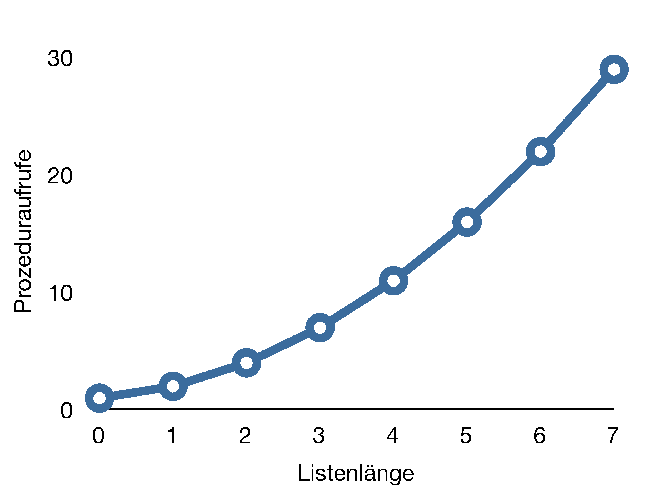
\includegraphics[width=0.5\textwidth]{invert-calls}
  \caption{Funktionaufrufe bei \texttt{invert}}
  \label{fig:invert-calls}
\end{figure}
%
Doch zurück zu \texttt{invert}.  Obwohl die zu erledigende Aufgabe
einfach erscheint, dauert schon das Invertieren von Listen der Länge
1000 eine ganze Weile.\footnote{So war es zumindest zur Zeit der
  Drucklegung dieses Buchs auf handelsüblichen Computern.  Ggf.\
  müssen es auf moderneren Rechnern Listen der Länge 10000 sein, um
  das Problem deutlich zu machen.}  
Tatsächlich ist es so, daß z.B.\
das Invertieren einer Liste der Länge 400 \emph{mehr} als doppelt so
lang wie das Invertieren einer Liste der Länge 200 benötigt.  Das
liegt daran, daß \texttt{invert} bei jedem rekursiven Aufruf
\texttt{append-element} aufruft, und \texttt{append-element} selbst
macht soviele rekursive Aufrufe wie die Liste lang ist.  Das wiederum
heißt aber, daß die Gesamtanzahl der Funktionaufrufe für das
Invertieren einer Liste der Länge $n$ so steigt wie in
der Kurve in Abbildung~\ref{fig:invert-calls} gezeigt, also offenbar
stärker als linear: Das erklärt das überproportionale Ansteigen der
Rechenzeit.  (Dafür ist auch Aufgabe~\ref{ref:o-of-invert} relevant.)
Dies ist für so eine einfache Aufgabe
inakzeptabel: Listen der Länge 10000 sind nichts ungewöhnliches, und
das Invertieren sollte dem Computer leichtfallen.

Tatsächlich gibt es eine bessere Methode, eine Liste umzudrehen: Die
obige \texttt{invert}"=Funktion konstruiert die Ergebnisliste, indem
stets Elemente \emph{hinten} angehängt werden.  Das entspricht 
nicht der "<natürlichen"> Konstruktion von Listen mit
\texttt{cons}, das ein Element \emph{vorn} anhängt.  
Das Ergebnis ließe sich aber durch Anhängen vorn ganz einfach
konstruieren, und zwar, indem in folgender Reihenfolge
Zwischenergebnisse\index{Zwischenergebnis} berechnet werden, wie in folgendem Beispiel für den
Testfall \texttt{(invert (list 1 2 3 4))}:
%
\begin{verbatim}
#<empty-list>
#<list 1>
#<list 2 1>
#<list 3 2 1>
#<list 4 3 2 1>
\end{verbatim}
%
Jedes Zwischenergebnis entsteht aus dem vorhergehenden, indem ein
Element vorn an die Liste darüber angehängt wird.  Dies geschieht in
der Reihenfolge, in der die Elemente in der ursprünglichen Liste
auftreten: scheinbar einfach.  Allerdings erlaubt die normale
Konstruktionsanleitung für Listen nicht, dieses Zwischenergebnis
mitzuführen: Das Ergebnis des rekursiven Aufrufs \texttt{(invert (rest
  lis))} ist unabhängig vom Wert von \texttt{(first lis)}.  Damit aber
ist es der Funktion aus der normalen Konstruktionsanleitung unmöglich,
die obige Folge von Zwischenergebnissen nachzuvollziehen, da von einem
Zwischenergebnis zum nächsten gerade \texttt{(first lis)} vorn
angehängt wird.  Für diesen speziellen Fall~-- wenn eine Berechnung das
Mitführen von Zwischenergebnissen erfordert~-- muß die normale
Konstruktionsanleitung deshalb angepaßt werden.

Dieses Problem läßt sich durch Mitführen des Zwischenergebnisses in
einem separaten Parameter lösen, dem sogenannten
\textit{Akkumulator\index{Akkumulator}}.  Dazu wird eine
Hilfsfunktion \texttt{invert-helper} definiert, die neben der Eingabeliste
diesen Akkumulator akzeptiert:
%
\begin{verbatim}
(: invert-helper ((list-of %a) (list-of %a) -> (list-of %a)))

(define invert-helper
  (lambda (lis acc)
    ...))
\end{verbatim}
%
Die Liste \texttt{lis} ist nach wie vor die bestimmende Eingabe, es
greifen also die entsprechenden Konstruktionsanleitungen für gemischte
und zusammengesetzte Daten:
%
\begin{verbatim}
(define invert-helper
  (lambda (lis acc)
    (cond
      ((empty? lis) ...)
      ((cons? lis)
       ... (first lis) ...
       ... (invert-helper (rest lis) ...) ...))))
\end{verbatim}
%
Wenn \texttt{invert-helper} aufgerufen wird, sind die noch zu
verarbeitenden Elemente der ursprünglichen Liste in \texttt{lis}, und
das Zwischenergebnis, was aus den Elementen davor berechnet wurde, ist
in \texttt{acc}.  Wenn \texttt{lis} leer ist, sind alle Elemente
verarbeitet und das Zwischenergebnis ist das Endergebnis:
%
\begin{verbatim}
(define invert-helper
  (lambda (lis acc)
    (cond
      ((empty? lis) acc)
      ((cons? lis)
       ... (first lis) ...
       ... (invert-helper (rest lis) ...) ...))))
\end{verbatim}
%
Für den rekursiven Aufruf muß noch ein neuer Wert für \texttt{acc}
übergeben werden.  Dieser entsteht, wie im Beispiel zu sehen ist,
dadurch, daß an den Akkumulator das erste Element der Liste vorn
angehängt wird:
%
\begin{verbatim}
(define invert-helper
  (lambda (lis acc)
    (cond
      ((empty? lis) acc)
      ((cons? lis)
       ... (invert-helper (rest lis)
                          (cons (first lis) acc)) ...))))
\end{verbatim}
%
Da der rekursive Aufrufs von \texttt{invert-helper} schließlich direkt das
Endergebnis zurückgegeben wird, ist damit die Funktion auch schon fertig:
%
\begin{verbatim}
(define invert-helper
  (lambda (lis acc)
    (cond
      ((empty? lis) acc)
      ((cons? lis)
       (invert-helper (rest lis)
                      (cons (first lis) acc))))))
\end{verbatim}
%
Die neue Hilfsfunktion \texttt{invert-helper} paßt nicht auf die Signatur
von \texttt{invert}; \texttt{invert} muß also separat definiert werden
und den passenden Anfangswert für \texttt{acc} übergeben:
%
\begin{verbatim}
(define invert
  (lambda (lis)
    (invert-helper lis empty)))
\end{verbatim}
%
% Da \texttt{invert-helper} ausschließlich als Hilfsfunktion zu
% \texttt{invert} benutzt wird und ohne \texttt{invert} keinen Nutzen
% hat, ist es nicht notwendig, eine separate Signatur für
% \texttt{invert-helper} anzugeben. HK: Wir haben aber schon eine Signatur
% dafür angegeben! ;-)

Die neue Version von \texttt{invert} kommt ohne
\texttt{append-element} aus.  Der Beispielaufruf von oben führt zu
folgender Auswertung im Substitutionsmodell, die sich auch im Stepper
gut nachvollziehen läßt:
%
\begin{alltt}\small
(invert \underline{(list 1 2 3 4)})
\(\Longrightarrow\ldots\Longrightarrow\) (\underline{invert-helper} #<list 1 2 3 4> empty)
\(\Longrightarrow\ldots\Longrightarrow\) (cond ((empty? #<list 1 2 3 4>) ...) ((cons? #<list 1 2 3 4>) ...))
\(\Longrightarrow\ldots\Longrightarrow\) (invert-helper (rest #<list 1 2 3 4>) (cons (first #<list 1 2 3 4>) empty))
\(\Longrightarrow\ldots\Longrightarrow\) (invert-helper #<list 2 3 4> (cons 1 empty))
\(\Longrightarrow\ldots\Longrightarrow\) (invert-helper #<list 2 3 4> #<list 1>)
\(\Longrightarrow\ldots\Longrightarrow\) (cond ((empty? #<list 2 3 4>) ...) ((cons? #<list 2 3 4>) ...))
\(\Longrightarrow\ldots\Longrightarrow\) (invert-helper (rest #<list 2 3 4>) (cons (first #<list 2 3 4>) #<list 1>))
\(\Longrightarrow\ldots\Longrightarrow\) (invert-helper #<list 3 4> (cons 2 #<list 1>))
\(\Longrightarrow\ldots\Longrightarrow\) (invert-helper #<list 3 4> #<list 2 1>)
\(\Longrightarrow\ldots\Longrightarrow\) (cond ((empty? #<list 3 4>) ...) ((cons? #<list 3 4>) ...))
\(\Longrightarrow\ldots\Longrightarrow\) (invert-helper (rest #<list 3 4>) (cons (first #<list 3 4>) #<list 2 1>))
\(\Longrightarrow\ldots\Longrightarrow\) (invert-helper #<list 4> (cons 3 #<list 2 1>))
\(\Longrightarrow\ldots\Longrightarrow\) (invert-helper #<list 4> #<list 3 2 1>)
\(\Longrightarrow\ldots\Longrightarrow\) (cond ((empty? #<list 4>) ...) ((cons? #<list 4>) ...))
\(\Longrightarrow\ldots\Longrightarrow\) (invert-helper (rest #<list 4>) (cons (first #<list 4>) empty))
\(\Longrightarrow\ldots\Longrightarrow\) (invert-helper #<empty-list> (cons 4 #<list 3 2 1>))
\(\Longrightarrow\ldots\Longrightarrow\) (invert-helper #<empty-list> #<list 4 3 2 1>)
\(\Longrightarrow\ldots\Longrightarrow\) (cond ((empty? #<empty-list>) #<list 4 3 2 1>) ((cons? #<empty-list>) ...))
\(\Longrightarrow\) #<list 4 3 2 1>
\end{alltt}
%
Tatsächlich arbeitet die neue Funktion auch effizienter: Da
\texttt{invert-helper} nicht bei jedem Aufruf selbst wieder eine Funktion
aufruft, die eine komplette Liste verarbeitet, steigt die Rechenzeit
nur noch proportional zur Länge der Liste.

Da die Funktion \texttt{invert} generell nützlich ist, ist sie unter
dem Namen \texttt{reverse\index{reverse@\texttt{reverse}}} fest eingebaut.

\begin{feature}{\texttt{letrec}}{scheme:letrec}
Die \texttt{letrec}-Form bindet lokale Variablen, ähnlich wie \texttt{let}.
Ihre Syntax ist mit der von \texttt{let} identisch.  Während bei \texttt{let}
die Variablen, die an die Werte der Ausdrücke gebunden werden,
in den Ausdrücken selbst nicht sichtbar sind, sind bei \texttt{letrec}\index{letrec@\texttt{letrec}}
die Bindungen sichtbar.  
\end{feature}

Die Funktion \texttt{invert-helper} wird nur an einer einzigen Stelle
aufgerufen, und zwar innerhalb von \texttt{invert}. Es würde auch kaum einen
Sinn ergeben, \texttt{invert-helper} von einer anderen Stelle aus
aufzurufen. Deshalb bietet es sich an, für \texttt{invert-helper} eine lokale
Definition zu verwenden, die nur innerhalb von \texttt{invert} sichtbar
ist. Dazu gibt es im Prinzip die \texttt{let}-Form, die allerdings für
diesen Zweck nicht verwendbar ist (Abb.~\ref{scheme:letrec}). Die dort
vorgestellte \texttt{letrec}-Form löst das Problem.

Akkumulatoren, die Zwischenergebnisse verwalten, sind bei der Lösung
einer Reihe von Problemen nützlich.  Zum Beispiel könnte eine
Funktion, welche die Fakultät $n!$ einer Zahl $n$ berechnet,
vorgehen, indem sie das Produkt $n \cdot \ldots \cdot 1$ schrittweise von
links her ausrechnet:
%
\begin{displaymath}
  \xymatrix@R=10pt@C=2pt{
      &       &   & & 1\ar@{-->}[dllll]\\
    1 & \cdot & 4 &=& 4\ar@{-->}[dllll]\\
    4 & \cdot & 3 &=& 12\ar@{-->}[dllll]\\
    12 & \cdot & 2 &=& 24\ar@{-->}[dllll]\\
    24 & \cdot & 1 &=& 24\ar@{-->}[dllll]\\
    24
    }
\end{displaymath}
%
Der Anfangswert für das Zwischenergebnis ist 1, also gerade die
Fakultät von 0.

Für die Konstruktion wird die Schablone für Funktionen, die natürliche
Zahlen verarbeiten, um einen Akkumulator erweitert:
\label{page:factorial-tail}
%
\begin{verbatim}
; Fakultät berechnen

(: ! (natural -> natural))

(check-expect (! 0) 1)
(check-expect (! 3) 6)
(check-expect (! 5) 120)

(define !
  (lambda (n)
    (letrec
        ((!-helper
          (lambda (n acc)
             (if (= n 0)
                acc
                ... ))))
      (!-helper n 1))))
\end{verbatim}
%
Wie aus der Beispielrechnung ersichtlich ist, wird aus dem "<alten">
Zwischenergebnis das "<neue"> Zwischenergebnis, indem jeweils
mit \texttt{n} multipliziert wird:
%
\begin{verbatim}
    (letrec
        ((!-helper
          (lambda (n acc)
             (if (= n 0)
                acc
        ... (!-helper (- n 1) (* n acc)) ...))))
\end{verbatim}
%
Wie schon bei \texttt{invert} ist es nicht notwendig, daß für die
noch verbleibenden Ellipsen etwas eingesetzt wird; das Programm ist
bereits fertig:
%
\begin{verbatim}
(: ! (natural -> natural))
(define !
  (lambda (n)
    (letrec
        ((!-helper
          (lambda (n acc)
             (if (= n 0)
                acc
                (!-helper (- n 1) (* n acc)) ...))))
      (!-helper n 1))))
\end{verbatim}
%
Tatsächlich ist es bei Funktionen mit Akkumulator grundsätzlich nicht
notwendig, für die Ellipsen am Schluß etwas einzusetzen. Bei der
normalen Schablone für Funktionen, die Listen bzw.\ natürliche Zahlen
verarbeiten, wird für diese Ellipsen Code eingesetzt, was das erste
Element der Liste mit dem Ergebnis des rekursiven Ausdrucks 
zum Rückgabewert kombiniert.  Dies ist beim Einsatz eines Akkumulators
aber nicht notwendig, da das erste Element der Liste bereits in die
Berechnung des nächsten Zwischenergebnisses eingeht und dieses
Zwischenergebnis beim letzten Aufruf bereits das Endergebnis ist.

\section{Schablonen für Funktionen mit Akkumulator}

Aus den beiden Beispielen des vorgehenden Abschnitts ergeben sich
direkt Schablonen für Funktionen mit Akkumulator.  Zunächst die
Schablone für Funktionen mit Akkumulator, die Listen akzeptieren:
%
\begin{alltt}
(: proc ((list-of elem) -> ...))

(define proc
  (lambda (lis)
    (letrec
       ((proc-helper
         (lambda (lis acc)
            (cond
              ((empty? lis) acc)
              ((cons? lis)
                 (proc-helper (rest lis)
                    (... (first lis) ... acc ...)))))))
    (proc-helper lis z))))
\end{alltt}
%
Hier ist \texttt{proc} der Name der zu definierenden Funktion
und \texttt{proc-helper} der Name der Hilfsfunktion mit
Akkumulator.  Der Anfangswert für den Akkumulator~-- also das initiale
Zwischenergebnis~-- ist der Wert von \texttt{z}.  Der
Ausdruck, der für \texttt{(... (first lis) ... acc ...)} einzusetzen
ist, macht aus dem alten Zwischenergebnis \texttt{acc} das neue
Zwischenergebnis.

Die Schablone für Funktionen mit Akkumulator, die natürliche Zahlen
akzeptieren, ist analog:
%
\begin{alltt}
(: proc (natural -> ...))

(define proc
  (lambda (n)
    (letrec
      ((proc-helper
        (lambda (n acc)
          (if (= n 0)
              acc
              (proc-helper (- n 1) (... acc ...))))))
    (proc-helper n z))))
\end{alltt}
%
Wieder ist \texttt{z} der Ausdruck für das initiale Zwischenergebnis
und für \texttt{(... acc ...)} ist ein Ausdruck einzusetzen, der aus
dem alten Zwischenergebnis \texttt{acc} ein neues macht.

\section{Minimum mit Akkumulator berechnen}
\label{sec:min-akku}

FIXME

\section{Kontext und Endrekursion}
\label{sec:iteration}

Ein Vergleich der beiden Versionen der Fakultätsfunktion von
S.~\pageref{page:factorial} und S.~\pageref{page:factorial-tail} zeigt, daß
Formulierungen mit und ohne Akkumulator
unterschiedliche Berechnungsprozesse erzeugen.  Hier ein Prozeß mit
Akkumulator:
%
\begin{alltt}
(! 4)
\(\Longrightarrow\) (!-helper 4 1)
\(\Longrightarrow\) (if (= 4 0) 1 (!-helper (- 4 1) (* 1 4)))
\(\Longrightarrow\) (if #f 1 (!-helper (- 4 1) (* 1 4)))
\(\Longrightarrow\) (!-helper (- 4 1) (* 1 4))
\(\Longrightarrow\) (!-helper 3 4)
\(\Longrightarrow\) (if (= 3 0) 4 (!-helper (- 3 1) (* 4 3)))
\(\Longrightarrow\) (if #f 4 (!-helper (- 3 1) (* 4 3)))
\(\Longrightarrow\) (!-helper (- 3 1) (* 4 3))
\(\Longrightarrow\) (!-helper 2 12)
\(\Longrightarrow\) (if (= 2 0) 12 (!-helper (- 2 1) (* 12 2)))
\(\Longrightarrow\) (if #f 12 (!-helper (- 2 1) (* 12 2)))
\(\Longrightarrow\) (!-helper (- 2 1) (* 12 2))
\(\Longrightarrow\) (!-helper 1 24)
\(\Longrightarrow\) (if (= 1 0) 24 (!-helper (- 1 1) (* 24 1)))
\(\Longrightarrow\) (if #f 24 (!-helper (- 1 1) (* 24 1)))
\(\Longrightarrow\) (!-helper (- 1 1) (* 1 24))
\(\Longrightarrow\) (!-helper 0 24)
\(\Longrightarrow\) (if (= 0 0) 24 (!-helper (- 0 1) (* 24 0)))
\(\Longrightarrow\) (if #t 24 (!-helper (- 0 1) (* 24 0)))
\(\Longrightarrow\) 24
\end{alltt}
%
Demgegenüber hier der Prozeß ohne Akkumulator:
%
\begin{alltt}
(! 4)
\(\Longrightarrow\) (if (= 4 0) 1 (* 4 (! (- 4 1))))
\(\Longrightarrow\) (if #f 1 (* 4 (! (- 4 1))))
\(\Longrightarrow\) (* 4 (! (- 4 1)))
\(\Longrightarrow\) (* 4 (! 3))
\(\Longrightarrow\) (* 4 (if (= 3 0) 1 (* 3 (! (- 3 1)))))
\(\Longrightarrow\) (* 4 (if #f 1 (* 3 (! (- 3 1)))))
\(\Longrightarrow\) (* 4 (* 3 (! (- 3 1))))
\(\Longrightarrow\) (* 4 (* 3 (! 2)))
\(\ldots\)
\(\Longrightarrow\) (* 4 (* 3 (* 2 (! 1))))
\(\Longrightarrow\) (* 4 (* 3 (* 2 (if (= 1 0) 1 (* 1 (! (- 1 1)))))))
\(\Longrightarrow\) (* 4 (* 3 (* 2 (if #f ... (* 1 (! (- 1 1)))))))
\(\Longrightarrow\) (* 4 (* 3 (* 2 (* 1 (! (- 1 1))))))
\(\Longrightarrow\) (* 4 (* 3 (* 2 (* 1 (! 0)))))
\(\Longrightarrow\) (* 4 (* 3 (* 2 (* 1 (if (= 0 0) 1 (* 0 (! (- 0 1))))))))
\(\Longrightarrow\) (* 4 (* 3 (* 2 (* 1 (if #t 1 (* 0 (! (- 0 1)))))))))
\(\Longrightarrow\) (* 4 (* 3 (* 2 (* 1 1))))
\(\Longrightarrow\) (* 4 (* 3 (* 2 1)))
\(\Longrightarrow\) (* 4 (* 3 2))
\(\Longrightarrow\) (* 4 6)
\(\Longrightarrow\) 24
\end{alltt}
%
Es ist deutlich sichtbar, daß die Version ohne Akkumulator alle
Multiplikationen bis zum Schluß "<aufstaut">.  Das heißt aber auch,
daß im Laufe des Berechnungsprozesses Ausdrücke auftauchen, die desto
größer werden je größer das Argument von \texttt{!} ist: Bei
\texttt{(!  100)} werden zum Beispiel 100 Multiplikationen aufgestaut.

Die Version mit Akkumulator hingegen scheint in der Größe der
zwischenzeitlich auftretenden Ausdrücke begrenzt zu sein.  Tatsächlich
stellt sich das Wachstum der Version ohne Akkumulator bei der Version
mit Akkumulator nicht ein.

Der Grund dafür sind die Schablonen: In der Schablone für Funktionen
ohne Akkumulator steht \texttt{(... (proc (- n 1)) ...)}, das
heißt, um den rekursiven Aufruf von \texttt{proc} wird noch
etwas "<herumgewickelt">, oder, anders gesagt, mit dem Ergebnis des
rekursiven Aufrufs passiert noch etwas.  Das, was mit dem Ergebnis
noch passiert, heißt der \textit{Kontext\index{Kontext}} des Aufrufs.
Bei \texttt{!} ist der vollständige Ausdruck \texttt{(* n (! (- n
  1)))}.  Wenn aus diesem Ausdruck der rekursive Aufruf \texttt{(! (-
  n 1))} herausgenommen wird, bleibt der Kontext \texttt{(* n
  \(\circ\))}, wobei $\circ$ markiert, wo der Aufruf entfernt
wurde.  Tatsächlich wird in der Literatur diese Markierung
\textit{Loch\index{Loch}} genannt und \texttt{[]} geschrieben.  Der
Kontext \texttt{(* n [])} macht deutlich, daß mit Ergebnis eines
Aufrufs, der später für \texttt{[]} eingesetzt wird, noch \texttt{n}
multipliziert wird.  Dementsprechend stauen sich in der
Reduktionsfolge die Multiplikationen mit den verschiedenen Werten von
\texttt{n}.

Bei der Fakultäts-Funktion mit Akkumulator ist der Ausdruck, zu dem
der Rumpf bei $\texttt{n} \neq 0$ reduziert wird, \texttt{(!-helper (- n 1)
  (* n acc))}.  Der Kontext des Aufrufs von \texttt{!-helper} innerhalb
dieses Ausdrucks ist \texttt{[]}, also \emph{leer}~-- \emph{nichts}
passiert mehr mit dem Rückgabewert von \texttt{!-helper}, und damit stauen
sich auch bei der Reduktion keine Kontexte an.  Solche Funktionaufrufe
ohne Kontext heißen \textit{endrekursiv\index{endrekursiv}}~-- eben,
weil nach dem rekursiven Aufruf "<Ende"> ist.\footnote{Das Konzept des
  Aufrufs ohne Kontext ist nicht auf rekursive Aufrufe beschränkt.  Im
  Englischen heißen solche Aufrufe allgemeiner \textit{tail
    calls\index{tail call}} (also ohne "<recursive">).}
Die Berechnungsprozesse, die von endrekursiven Aufrufen generiert
werden, heißen auch \textit{iterative\index{Iteration}} Prozesse.

\section{Das Phänomen der umgedrehten Liste}

Die beiden Varianten der Fakultäts-Funktion berechnen zwar beide 
stets das gleiche Ergebnis.  Die beiden Reduktionsfolgen für
\texttt{(! 4)} aus dem vorigen Abschnitt zeigen allerdings, daß die
beiden Funktionen bei der Berechnung unterschiedlich vorgehen:
Während die Variante ohne Akkumulator "<von rechts"> multipliziert,
also folgendermaßen auswertet:
%
\begin{displaymath}
  4\cdot (3 \cdot (2 \cdot (1 \cdot 1)))
\end{displaymath}
%
multipliziert die Variante mit Akkumulator "<von links">:
%
\begin{displaymath}
  (((1 \cdot 4)\cdot 3)\cdot 2)\cdot 1
\end{displaymath}
%
Die Multiplikationen passieren also in umgekehrter Reihenfolge.
Dies macht bei der Fakultät keinen Unterschied, da die Multiplikation
assoziativ ist.  Diese Assoziativität ist jedoch nicht immer
gegeben~-- insbesondere nicht bei Funktionen, die Listen zurückgeben.
Hier zum Beispiel eine Funktion, die eine Zahl $n$ akzeptiert und eine
absteigende Liste der Zahlen von $n$ bis $1$ zurückliefert:
%
\begin{verbatim}
; Liste der Zahlen von n bis 1 generieren
(: build-list (natural -> (list-of natural)))

(check-expect (build-list 0) empty)
(check-expect (build-list 3) (list 3 2 1))

(define build-list
  (lambda (n)
    (if (= n 0)
        empty
        (cons n (build-list (- n 1))))))
\end{verbatim}
%
Die direkte Übersetzung in eine Variante mit Akkumulator liefert:
%
\begin{verbatim}
(define build-list
  (lambda (n)
    (letrec
      ((build-list-helper
        (lambda (n acc)
          (if (= n 0)
              acc
              (build-list-helper (- n 1) (cons n acc))))))
    (build-list-helper n empty))))
\end{verbatim}
%
Diese Variante ist inkorrekt: Sie liefert z.B.\ für
\texttt{(build-list 3)} das Ergebnis \verb|#<list 1 2 3>|, die
Elemente der Liste sind also in umgekehrter Reihenfolge.  Da schon die
Fakultätsfunktion mit Akkumulator die Multiplikationen gegenüber der
Variante ohne Akkumulator in umgekehrter Reihenfolge durchgeführt hat, war dies allerdings zu
erwarten, und ist ein generelles Phänomen bei der Berechnung von
Listen-Ausgaben mit Akkumulator.  Das Problem kann durch das Umdrehen
der Ergebnisliste gelöst werden:
%
\begin{verbatim}
    (letrec
      ((build-list-helper
        (lambda (n acc)
          (if (= n 0)
              (reverse acc)
              (build-list-helper (- n 1) (cons n acc))))))
\end{verbatim}
%


\section*{Anmerkungen}

Bei der Auswertung von Programmen durch den Computer wird für die
Verwaltung von Kontexten Speicherplatz benötigt: Bei rekursiven
Funktionen ohne Akkumulator wächst dieser Speicherplatz mit der Größe
der Argumente.  Entsprechend wird prinzipiell kein Speicherplatz
benötigt, wenn kein Kontext anfällt.  In den Lehrsprachen  wird auch tatsächlich
kein Speicherplatz für endrekursive Aufrufe verbraucht; dies ist
allerdings bei vielen anderen Programmiersprachen nicht der Fall.
Mehr dazu in Kapitel~\ref{cha:secd}.

\section*{Aufgaben}

\begin{aufgabe}
  \label{ref:o-of-invert}
  Entwicklen Sie eine Formel für die Anzahl der rekursiven Aufrufe in
  der ersten Version von \texttt{invert}!  (Hinweis: Greifen Sie auf
  die Gauß'sche Summenformel zurück.)
\end{aufgabe}

\begin{aufgabe}
  Schreiben Sie eine Funktion \texttt{list-sum+product}, die eine
  Liste von Zahlen akzeptiert und eine zweielementige Liste
  zurückgibt, deren erstes Element die Summe der Listenelemente und
  deren zweites Element ihr Produkt ist.  Schreiben Sie zwei Varianten
  der Funktion: eine ohne Akkumulator und eine mit zwei Akkumulatoren.
\end{aufgabe}

\begin{aufgabe}
  Schreiben Sie eine Funktion, die als Eingabe eine Liste von Kursen
  einer Aktie (als Zahlen) eines Tages akzeptiert (nach Tageszeit
  aufsteigend sortiert), und als Rückgabewert den höchstmöglichen
  Gewinn liefert, die durch den Kauf und folgenden Verkauf der Aktie
  an diesem Tag erreicht werden kann.

  Hinweis: Diese Funktion benötigt zwei Akkumulatoren.
\end{aufgabe}

\begin{aufgabe}
  Schreibe zu der Funktion \texttt{power} aus Aufgabe~\ref{aufg:power} eine
  endrekursive Variante.
\end{aufgabe}

\begin{aufgabe}
  Identifizieren Sie die Kontexte der Aufrufe der Funktionen namens
  \texttt{p} in folgenden Ausdrücken:
  
\begin{verbatim}
(+ (p (- n 1)) 1)
(p (- n 1) acc)
(* (p (rest lis)) b)
(+ (* 2 (p (- n 1))) 1)
(p (- n 1) (* acc n))
(f (p n))
(+ (f (p n)) 5)
(p (f (- n 1)) (* n (h n))) 
(+ (f (p n)) (h n))
\end{verbatim}
  %
  Welche Aufrufe sind endrekursiv bzw.\ \textit{tail calls}?
\end{aufgabe}

\begin{aufgabe}
  Schreibe eine endrekursive Variante von \texttt{list-length}.
\end{aufgabe}

\begin{aufgabe}
  Schreibe eine endrekursive Variante von
  \texttt{concatenate}.  Falls du Hilfsfunktionen auf
  Listen dafür benutzt, gib auch dafür endrekursive Definitionen an.
\end{aufgabe}

\begin{aufgabe}
  Schreibe endrekursive Varianten von \texttt{evens} und \texttt{odds}
  aus Aufgabe~\ref{ex:evensodds} auf Seite~\pageref{ex:evensodds}.
  Falls du Hilfsfunktionen auf Listen dafür benutzt, gib auch dafür
  endrekursive Definitionen an.
\end{aufgabe}

\begin{aufgabe}
  \lstinline{List-fold} sammelt die Elemente von hinten nach vorn bzw.
  von rechts nach links auf, entsprechend der "<natürlichen">
  Rekursionsstruktur über Listen.  Das gleiche Spiel lässt sich auch in
  der anderen Richtung durchführen.  Heraus kommt eine Funktion
  \lstinline{list-fold-left}, die folgende Gleichung (in
  Infix-Schreibweise) erfüllt:
  % 
\begin{lstlisting}
(list-fold-left |\(u\)| |\(\odot\)| (|\(a_1\)| |\(\ldots\)| |\(a_n\)|)) = |\((\ldots((u\odot a_1)\odot a_2)\ldots\odot a_n)\)|
\end{lstlisting}
  % 
  Programmiere \lstinline{list-fold-left}!
\end{aufgabe}

\begin{aufgabe}
  Programmiere eine Version von
  \lstinline{list-fold-left}, nämlich die Funktion
  \lstinline{list-fold-left-bonus}, die \lstinline{list-fold} benutzt aber
  selbst keine Rekursion enthält und auch keine rekursiven
  Hilfsfunktionen aufruft.
\end{aufgabe}


\begin{aufgabe}
  Das Newton-Verfahren dient zur nährungsweisen
  Berechnung von Nullstellen. Für ein gegebenen Startwert nähert sich die
  Iteration 
  \begin{displaymath}
    x_{n+1} = x_n - \frac{f(x_n)}{f'(x_n)}
  \end{displaymath}
  immer näher an eine Nullstelle an.

  Programmiere das Newton-Verfahren!
  
  Hinweis: Die Lösung soll gut genug sein, wenn der Funktionswert nahe
  bei 0 liegt, also kleiner als eine Toleranz ist. 
  Da das
  Newton-Verfahren nicht immer eine Lösung liefert, programmiere
  Deine Funktion so, dass sie nach einer gewissen Anzahl von Schritten
  automatisch abbricht und \lstinline{#f} zurück gibt.
\end{aufgabe}


%%% Local Variables: 
%%% mode: latex
%%% TeX-master: "i1"
%%% End: 



% Diese Datei ist Teil des Buchs "Schreibe Dein Programm!"
% Das Buch ist lizensiert unter der Creative-Commons-Lizenz
% "Namensnennung 4.0 International (CC BY 4.0)"
% http://creativecommons.org/licenses/by/4.0/deed.de

\chapter{Zeitabhängige Modelle}
\label{cha:representation-and-state}

TBD

\section{Das Teachpack \texttt{image2.ss}}

Für die Grafikprogrammierung mit \drscheme{} ist es notwendig, ein
sogenanntes \textit{Teachpack\index{Teachpack}} zu laden~-- ein
kleiner Sprachzusatz, in diesem Fall mit einer Reihe von Funktionen zur Erzeugung von
Bildern.  Dazu muß im Menü \texttt{Sprache} (oder \texttt{Language} in
der englischen Ausgabe) der Punkt \texttt{Teachpack hinzufügen}
(\texttt{Add teachpack}) angewählt werden, und im dann erscheinenden
Auswahl-Dialog im Verzeichnis \texttt{deinprogramm} die Datei
\texttt{image22.ss\index{image2.ss@\texttt{image2.ss}}}.

Im Teachpack \texttt{image2.ss} erzeugen verschiedene Funktionen
einfache Bilder.  So hat z.B.\ die Funktion \texttt{rectangle}
folgende Signatur:\index{rectangle@\texttt{rectangle}}
%
\begin{alltt}
(: rectangle (natural natural mode color -> image))
\end{alltt}
%
Dabei sind die ersten beiden Argumente Breite und Höhe eines Rechtecks
in Pixeln.
Das Argument von der Sorte \texttt{mode}\index{mode@\texttt{mode}} ist eine Zeichenkette, die
entweder \verb|"solid"| oder \verb|"outline"| sein muß. Sie bestimmt,
ob das Rechteck als durchgängiger Klotz oder nur als Umriß gezeichnet
wird.  Das Argument von der Sorte \texttt{color}\index{color@\texttt{color}} ist eine
Zeichenkette, die eine Farbe (auf Englisch) bezeichnet, 
zum Beispiel \verb|"red"|, \verb|"blue"|, \verb|"yellow"|,
\verb|"black"|, \verb|"white"| oder \verb|"gray"|.  Als Ergebnis
liefert \texttt{rectangle} ein Bild, das von der \drscheme{}-REPL
entsprechend angezeigt wird wie andere Werte auch.

\begin{figure}[tb!]
  \centering
  TBD
  \caption{Teachpack \texttt{image2.ss}}
  \label{fig:image-ss}
\end{figure}

Es gibt es noch weitere Funktionen, die 
geometrische Figuren zeichnen:\index{circle@\texttt{circle}}
%
\begin{alltt}
(: circle (natural mode color -> image))
\end{alltt}
%
Die \texttt{circle}-Funktion liefert einen Kreis, wobei das erste
Argument den Radius angibt.  Die \texttt{mode}- und
\texttt{color}-Argumente sind wie bei \texttt{rectangle}.
%
\begin{alltt}
(: ellipse (natural natural mode color -> image))
\end{alltt}
%
\index{ellipse@\texttt{ellipse}}Diese Funktion liefert eine Ellipse,
wobei das erste Argument die Breite und das zweite die Höhe angibt.
%
\begin{alltt}
(: triangle (natural mode color -> image))
\end{alltt}
%
\index{triangle@\texttt{triangle}}Diese Funktion liefert ein nach oben
zeigendes gleichseitiges Dreieck, wobei das erste Argument die
Seitenlänge angibt.
%
\begin{alltt}
(: line (natural natural real real real real color -> image))
\end{alltt}
%
\index{line@\texttt{line}}zeichnet eine Linie.  Der Aufruf
\texttt{(line $w$ $h$ $x_1$ $y_1$ $x_2$ $y_2$ $c$)} liefert ein Bild
mit Breite $w$ und Höhe $h$, in dem eine Linie von $(x_1, y_1)$ nach
$(x_2, y_2)$ läuft.  Der Ursprung $(0,0)$ ist links \emph{oben},
also nicht, wie in der Mathematik üblich, links unten.

Da diese geometrischen Formen für sich genommen langweilig sind, können
mehrere Bilder miteinander kombiniert werden.

Zum Aufeinanderlegen gibt es die Funktion \texttt{overlay\index{overlay@\texttt{overlay}}}:
%
\begin{alltt}
(: overlay (image image h-place v-place -> image))
\end{alltt}
%
Dabei sind die ersten beiden Argumente die Bilder, die
aufeinandergelegt werden~-- das zweite auf das erste.
Die beiden anderen Argumente geben an, wie
die beiden Bilder zueinander positioniert werden.  Die Signatur
von \texttt{h-place}, das die horizontale Positionierung festlegt,
ist:\index{h-place@\texttt{h-place}}
%
\begin{alltt}
(define h-place
   (signature
      (mixed natural
             (one-of "left"
                     "right"
                     "center"))))
\end{alltt}
%
Im ersten Fall, wenn es sich um eine Zahl $x$ handelt, wird das zweite
Bild $x$ Pixel vom linken Rand auf das erste gelegt.  Die drei
Fälle mit Zeichenketten sagen, daß die Bilder am linken Rand bzw.\ am
rechten Rand bündig plaziert werden, bzw.\ das zweite Bild horizontal
in die Mitte des ersten gesetzt wird.
Dementsprechend ist
\texttt{v-place}, das die vertikale Positionierung festlegt,
wie folgt definiert:\index{v-place@\texttt{v-place}}
%
\begin{alltt}
(define h-place
   (signature
      (mixed natural
             (one-of "top"
                     "bottom"
                     "center"))))
\end{alltt}
%
Im ersten Fall, wenn es sich um eine Zahl $y$ handelt, wird das zweite
Bild $y$ Pixel vom oberen Rand auf das erste gelegt.  Die drei
Fälle mit Zeichenketten sagen, daß die Bilder am oberen Rand bzw.\ am
unteren Rand bündig plaziert werden, bzw.\ das zweite Bild vertikal
in die Mitte des ersten gesetzt wird.

Das Bild, das bei \texttt{overlay} herauskommt, ist groß genug, daß
beide Eingabebilder genau hineinpassen.

Die folgenden Hilfsprozeduren sind Spezialfälle von \texttt{overlay}:
%
\begin{alltt}
(: above  (image image h-mode -> image))
(: beside (image image v-mode -> image))
\end{alltt}
%
Die Funktion \texttt{above\index{above@\texttt{above}}} ordnet zwei
Bilder übereinander an, \texttt{beside\index{beside@\texttt{beside}}}
nebeneinenander.  Dabei ist \texttt{h-mode} eine der Zeichenketten
\verb|"left"|, \verb|"right"| und \verb|"center"|, die angibt, ob die
Bilder bei \texttt{above} an der linken oder rechten Kante oder der
Mitte ausgerichtet werden.  Entsprechend ist \texttt{v-mode} eine der
Zeichenketten \verb|"top"|, \verb|"bottom"| und \verb|"center"|, die
angibt, ob die Bilder bei \texttt{beside} oben, unten oder an der
Mitte ausgerichtet werden.

Die Funktionen \texttt{clip} und \texttt{pad} beschneiden bzw.\
erweitern ein Bild:\index{clip@\texttt{clip}}\index{pad@\texttt{pad}}
%
\begin{alltt}
(: clip (image natural natural natural natural -> image))
(: pad  (image natural natural natural natural -> image))
\end{alltt}
%
Ein Aufruf \texttt{(clip $i$ $x$ $y$ $w$ $h$)} liefert 
das Teilrechteck des Bildes $i$ mit Ecke bei $(x, y)$, Breite $w$ und
Höhe $h$.  Der Aufruf \texttt{(pad $i$ $l$ $r$ $t$ $b$)}
fügt an den Seiten von $i$ noch transparenten Leerraum an: $l$ Pixel
links, $r$ Pixel rechts, $t$ Pixel oben und $b$ Pixel unten.

Abbildung~\ref{fig:image-ss} zeigt, wie sich die einige der
\texttt{image.ss}-Funktionen in der \drscheme{}-REPL verhalten.

\begin{figure}
  \centering
  TBD
  \caption{Eingefügte Bilder in der \drscheme{}-REPL}
  \label{fig:image-insert}
\end{figure}
%
Es ist auch möglich, externe Bilder-Dateien in
\texttt{image2.ss}-Bilder zu verwandeln.  Dazu dient der Menüpunkt
\texttt{Bild einfügen} im \texttt{Spezial}-Menü:  \drscheme{} fragt nach dem
Namen einer Bilddatei, die dann in den Programmtext da eingefügt wird,
wo der Cursor steht.  Die eingefügten Bilder dienen dann als
Literale für Bild-Objekte.  Abbildung~\ref{fig:image-insert} zeigt ein
Beispiel.

Die folgenden Funktionen ermitteln Breite und Höhe
eines Bildes:\index{image-width@\texttt{image-width}}\index{image-height@\texttt{image-height}}
%
\begin{alltt}
(: image-width  (image -> natural))
(: image-height (image -> natural))
\end{alltt}

\section{Zwischenergebnisse benennen}
\label{sec:let}

\index{lokale Variable}\index{Variable!lokal} Im nächsten Abschnitt
geht es um ein etwas umfangreicheres Programm mit vielen
\textit{Zwischenergebnissen}\index{Zwischenergebnis}.  Die
\texttt{let}-Form erlaubt, Zwischenergebnisse zu benennen und beliebig
oft zu verwenden.  Abbildung~\ref{scheme:let} erläutert die
Funktionsweise.
%
\begin{feature}{Lokale Variablen mit \texttt{let}}{scheme:let}
\texttt{Let}\index{let@\texttt{let}} ist für das Anlegen \textit{lokaler
  Variablen}\index{lokale Variable}\index{Variable!lokal} zuständig.  Ein \texttt{let}-Ausdruck hat die folgende
allgemeine Form:
%
\begin{alltt}
(let ((\(v\sb{1}\) \(e\sb{1}\)) \(\ldots\) (\(v\sb{n}\) \(e\sb{n}\))) \(b\))
\end{alltt}
%
Dabei müssen die $v_i$ Variablen sein und die $e_i$ und
$b$ (der \textit{Rumpf})\index{Rumpf} beliebige Ausdrücke.  Bei der Auswertung
eines solchen \texttt{let}-Ausdrucks werden zunächst alle $e_i$
ausgewertet.  Dann werden deren Werte für die Variablen $v_i$ im Rumpf
eingesetzt; dessen Wert wird dann zum Wert des \texttt{let}-Ausdrucks.

Ein \texttt{let}-Ausdruck hat die gleiche Bedeutung wie folgende
Kombination aus Lambda-Ausdruck und Applikation:
%
\begin{alltt}
(let ((\(v\sb{1}\) \(e\sb{1}\)) \(\ldots\) (\(v\sb{n}\) \(e\sb{n}\))) \(b\))
\(\mapsto\) ((lambda (\(v\sb{1}\) \(\ldots\) \(v\sb{n}\)) \(b\)) \(e\sb{1}\) \(\ldots\) \(e\sb{n}\))
\end{alltt}
%
\end{feature}
%
\texttt{Let} ist selbst dann nützlich, wenn ein Zwischenergebnis nicht
mehrfach verwendet wird.  Es kann die Lesbarkeit des Programmtextes
erhöhen, besonders wenn ein aussagekräftiger Name verwendet wird.
Zum Beispiel berechnet die folgende Funktion das Materialvolumen eines
Rohrs, von dem Außenradius, Dicke und Höhe angegeben sind:\index{pipe-volume@\texttt{pipe-volume}}
%
\begin{alltt}
; Materialvolumen eines Rohrs berechnen
(: pipe-volume (number number number -> number))
(define pipe-volume
  (lambda (outer-radius thickness height)
    (let ((inner-radius (- outer-radius thickness)))
      (- (cylinder-volume outer-radius height)
         (cylinder-volume inner-radius height)))))
\end{alltt}
%
In diesem Beispiel wird eine einzelne lokale Variable namens
\texttt{inner-radius} eingeführt, die für den Wert von \texttt{(-
  outer-radius thickness)} steht.

Da die Variablen, die durch \texttt{let} und \texttt{lambda} gebunden
werden, nur jeweils im Rumpf des \texttt{let} bzw.\ \texttt{lambda}
gelten, heißen sie auch \textit{lokale Variablen}.  Die durch
\texttt{define} gebundenen Variablen heißen dementsprechend~-- da sie überall
gelten~-- \textit{globale Variablen\index{Variable!global}\index{globale Variable}}.

\texttt{Let} kann auch mehrere lokale Variablen
gleichzeitig einführen, wie im folgenden Beispiel:
%
\begin{alltt}
(let ((a 1)
      (b 2)
      (c 3))
  (list a b c))
\evalsto{} #<list 1 2 3>
\end{alltt}
%
Bei der Benutzung von \texttt{let} ist zu beachten, daß die Ausdrücke,
deren Werte an die Variablen gebunden werden, allesamt
\emph{außerhalb} des Einzugsbereich des \texttt{let} ausgewertet
werden.  Folgender Ausdruck führt also bei der Auswertung zu einer
Fehlermeldung:
%
\begin{alltt}
(let ((a 1)
      (b (+ a 1)))
  b)
\evalsto{} reference to an identifier before its definition: a
\end{alltt}
%

\begin{mantra}[lokale Variablen]\label{mantra:local-variables}
    Benenne Zwischenergebnisse mit lokalen Variablen.

\end{mantra}

\section{Modelle und Ansichten}


TBD

\section{Bewegung und Zustand}

TBD  Dafür ist ein weiteres Teachpack namens
\texttt{universe.ss}\index{universe.ss@\texttt{universe.ss}} zuständig.  Es
kann in \drscheme{} genauso wie bei \texttt{image2.ss}
geladen werden.  

Alle Definitionen von
\texttt{image2.ss} sind auch in \texttt{universe.ss} verfügbar.

In der Terminologie von \texttt{universe.ss} ist ein Modell eine
\textit{world}, auf deutsch eine \textit{Welt}: Die Idee dahinter
ist, daß ein Bild eine Ansicht einer kleinen Welt ist.  Damit das
funktioniert, muß bei \texttt{universe.ss} eine erste Welt angemeldet
werden, zusammen mit Angaben, wie groß die Ansicht wird.  Dazu gibt es
die Funktion \texttt{big-bang}\index{big-bang@\texttt{big-bang}}:
%
\begin{alltt}
(: big-bang (natural natural number world -> #t))
\end{alltt}
%
("`Big Bang"' heißt zu deutsch "`Urknall"'.)
Die ersten beiden Argumente geben Breite und Höhe der Ansicht an.  Das
dritte Argument gibt die Dauer (in Sekunden) zwischen Ticks der Uhr
an, die für die Animation benötigt wird.  Das vierte Argument gibt
schließlich die erste Welt an.  (Der Rückgabewert, immer
\verb|#t|, ist ohne Bedeutung.)  Für den Himmel mit
Sonne sieht der Aufruf von \texttt{big-bang} folgendermaßen aus:
%
\begin{alltt}
(big-bang sky-width sky-height 0.1 0)
\end{alltt}
%
Dieser Aufruf erzeugt ein Fenster mit Breite und Höhe des Himmels,
startet die Uhr, die jede Sekunde zehnmal tickt, und legt als erste
Welt "`0"', also den Anfang der Zeit fest.  (Eine zehntel Sekunde
reicht etwa aus, damit die Animation dem menschlichen Auge als
"`Bewegung"' erscheint.)

Damit das Teachpack die Welt in eine Ansicht umwandeln kann, muß eine
entsprechende Ansicht angemeldet werden.  Dafür ist die Funktion
\texttt{on-redraw\index{on-redraw@\texttt{on-redraw}}} zuständig:
%
\begin{alltt}
(: on-redraw ((world -> image) -> #t))
\end{alltt}
%
Als Argument akzeptiert \texttt{on-redraw} also eine Funktion, die aus
einer Welt ein Bild macht.  TBD

Auch diese Funktion muß noch beim Teachpack angemeldet werden.  Dafür
die Teachpack-Funktion
\texttt{on-tick-event\index{on-tick-event@\texttt{on-tick-event}}}
zuständig:
%
\begin{alltt}
(: on-tick-event ((world -> world) -> #t))
\end{alltt}
%
Die \texttt{on-tick-event}-Funktion akzeptiert eine Funktion, die bei
jedem Uhren-Tick aufgerufen wird, um aus der "`alten"' Welt eine neue
zu machen.  Auf diese Beschreibung und auch auf die Signatur
paßt aber \texttt{next-time}.  Der Aufruf kann also so aussehen:
%
\begin{alltt}
(on-tick-event next-time)
\end{alltt}
%
Wenn das Programm
beendet werden soll, muß \texttt{on-tick-event} die Funktion
\texttt{end-of-time\index{end-of-time@\texttt{end-of-time}}} des
Teachpacks aufrufen, die folgende Signatur hat:
%
\begin{alltt}
(: end-of-time (string -> world))
\end{alltt}
%

\section{Andere Welten}

Eine kleine (wenn auch nicht besonders sinnvolle) Erweiterung zeigt,
wie die Animation auf Benutzereingaben reagieren kann.  Dazu muß sie
noch eine weitere Funktion anmelden, und zwar mittels
\texttt{on-key-event\index{on-key-event@\texttt{on-key-event}}}, das
ähnlich funktioniert wie \texttt{on-tick-event}:
%
\begin{alltt}
(: on-key-event ((world string -> world) -> #t))
\end{alltt}
%
Die Funktion, die mit \texttt{on-key-event} angemeldet wird, wird
immer aufgerufen, wenn der Benutzer eine Taste drückt.  Welche Taste
gedrückt wurde, gibt das zweite Argument 
an.  Wenn der Benutzer eine reguläre Zeichen-Taste drückt (also keine
Cursor-Taste o.ä.), ist dieses Argument eine Zeichenkette bestehend
aus diesem einen Zeichen.

TBD

\section*{Aufgaben}

TBD

\begin{aufgabe}
  Schreiben Sie ein kleines Telespiel Ihrer Wahl.
\end{aufgabe}

%%% Local Variables: 
%%% mode: latex
%%% TeX-master: "i1"
%%% End: 



% Diese Datei ist Teil des Buchs "Schreibe Dein Programm!"
% Das Buch ist lizensiert unter der Creative-Commons-Lizenz
% "Namensnennung 4.0 International (CC BY 4.0)"
% http://creativecommons.org/licenses/by/4.0/deed.de

\chapter{Eigenschaften von Funktionen}
\label{cha:properties}

Daß $1+1$ gleich $2$ ist, ist ein \textit{Beispiel} für die
Arbeitsweise der Addition.  Dieses Beispiel könnte auch als Testfall
für eine programmierte Version der Addition durchgehen.  Unter
Umständen kann ein Beispiel, als Testfall formuliert, einen Fehler in
einem Programm finden.  Allerdings ist das Formulieren von Beispielen
mühsam.  Schlimmer noch, eine Menge von Testfällen reicht nur selten
aus, um die Korrektheit einer Funktion auch zu garantieren: Die
Testfälle decken meist nicht alle möglichen Anwendungen einer Funktion
ab.  Darum ist es oft sinnvoll, statt isolierter Beispiele allgemeine
Eigenschaften zu formulieren und zu überprüfen~-- am besten sogar,
diese zu beweisen.  Dieses Kapitel zeigt, wie das geht.

\section{Eigenschaften von eingebauten Operationen}

In diesem Abschnitt wird die Formulierung und Überprüfung von
Eigenschaften anhand von bekannten eingebauten Operationen wie
\texttt{+}, \texttt{and}, \texttt{=} etc.\ demonstriert.

\subsection{Binäre Operationen}
\label{sec:eigenschaften-binaere-operationen}

Eine allgemein bekannte Eigenschaft der Addition ist die
\index{Kommutativität}\textit{Kommutativität}:
%
\begin{displaymath}
a + b = b + a
\end{displaymath}
%
Auch wenn intuitiv die Bedeutung klar ist, ist  die Eigenschaft genau
genommen so noch nicht präzise schriftlich festgehalten, da nicht
notiert ist, was $a$ und $b$ sind: Die Idee ist natürlich,
daß $a$ und $b$ beliebige \emph{Zahlen} sind.  Im allgemeinen also:
%
\begin{displaymath}
\forall a \in \mathbb{C}, b \in \mathbb{C}:\ a + b = b + a 
\end{displaymath}
%
(Wer sich mit der Vorstellung komplexer Zahlen nicht wohlfühlt, kann
das $\mathbb{C}$ auch durch $\mathbb{R}$ oder $\mathbb{Q}$ ersetzen.)

\begin{feature}{\texttt{for-all}}{scheme:for-all}
  \texttt{For-all}\index{for-all@\texttt{for-all}} ermöglicht das
  Formulieren von \textit{Eigenschaften\index{Eigenschaft}}.  Ein
  \texttt{for-all}-Ausdruck hat die folgende allgemeine Form:
%
\begin{alltt}
(for-all ((\(v\sb{1}\) \(c\sb{1}\)) \(\ldots\) (\(v\sb{n}\) \(c\sb{n}\))) \(b\))
\end{alltt}
%
Dabei müssen die $v_i$ Variablen sein, die $c_i$ Signaturen und $b$ (der
Rumpf) ein Ausdruck, der entweder einen booleschen Wert oder eine
Eigenschaft liefert.  Der \texttt{for-all}-Ausdruck hat als Wert eine
Eigenschaft, die besagt, daß \(b\) gilt für \emph{alle} Werte der
$v_i$, welche die Signaturen $c_i$ erfüllen.
\end{feature}

In Scheme läßt sich diese Eigenschaft für die eingebaute Funktion
\texttt{+} aufschreiben~-- das $\forall$ ist auf
Tastaturen nicht vertreten und wird darum ausgeschrieben (siehe
Abbildung~\ref{scheme:for-all}):
%
\begin{alltt}
(for-all ((a number)
          (b number))
  (= (+ a b) (+ b a)))
\end{alltt}
%
Das Ergebnis dieses Ausdrucks wird in der REPL etwas undurchsichtig
angezeigt:
%
\begin{alltt}
\evalsto{} #<:property>
\end{alltt}
%
\begin{feature}{\texttt{check-property}}{scheme:check-property}

\texttt{Check-property}\index{check-property@\texttt{check-property}}
testet eine Eigenschaft analog zu \texttt{check-expect}.  Eine
\texttt{check"=property}"=Form sieht so aus:
%
\begin{alltt}
(check-property \(e\)) 
\end{alltt}
%
$e$ ist ein Ausdruck, der eine Eigenschaft liefern muß~-- in der Regel
also ein \texttt{for-all}-Ausdruck.

Bei der Auswertung setzt \texttt{check-property} für die Variablen der
\texttt{for-all}-Ausdrücke verschiedene Werte ein und testet, ob die
Eigenschaft jeweils erfüllt ist.

\texttt{Check-property} funktioniert nur für Eigenschaften, bei denen
aus den Signaturen sinnvoll Werte generiert werden können.  Dies ist
für die meisten eingebauten Signaturen der Fall, aber nicht für
Signaturvariablen und Signaturen, die mit \texttt{predicate},
\texttt{property} oder \texttt{define-record-procedures} definiert
wurden.
\end{feature}
%
Bessere Informationen lassen sich erzielen, wenn \texttt{for-all}-Ausdrücke in
eine  \texttt{check-property}-Form
(siehe Abbildung~\ref{scheme:check-property}) eingebettet werden:
%
\begin{alltt}
(check-property
  (for-all ((a number)
            (b number))
    (= (+ a b) (+ b a))))
\end{alltt}
%
\texttt{Check-property} fungiert, wie \texttt{check-expect} oder
\texttt{check-within}, als Testfall und wird auch als solcher
ausgewertet.  Da \texttt{+} tatsächlich kommutativ ist, läuft der
Testfall auch anstandslos durch.

Interessanter wird es erst bei Eigenschaften, die nicht stimmen.  Zum
Beispiel ist die Subtraktion \texttt{-} nicht kommutativ:
%
\begin{alltt}
(check-property
 (for-all ((a number)
           (b number))
   (= (- a b)
      (- b a))))
\end{alltt}
%
Hierfür liefert \drscheme{} folgende Meldung:
%
\begin{alltt}
        Eigenschaft falsifizierbar mit a = \framebox{0.0} b = \framebox{-1.5}
\end{alltt}
%
\textit{Falsifizierbar}\index{falsifizierbar} bedeutet, daß es ein
\textit{Gegenbeispiel\index{Gegenbeispiel}} für die Eigenschaft gibt,
also Werte für die Variablen \texttt{a} und \texttt{b}, welche die
Eigenschaft falsch werden lassen.  \drscheme{} hat in diesem Fall ein
Gegenbeispiel gefunden, bei dem \texttt{a} den Wert $0.0$ und
\texttt{b} den Wert $1.5$ hat:
%
\begin{alltt}
(- 0.0 -1.5)
\evalsto{} 1.5
(- -1.5 0.0)
\evalsto{} -1.5
\end{alltt}
%
Dieses Beispiel widerlegt also tatsächlich die Behauptung der Eigenschaft.

Hinter den Kulissen hat \drscheme{} verschiedene Werte für \texttt{a} und
\texttt{b} durchprobiert und in die Eigenschaft eingesetzt, also effektiv
nach einem Gegenbeispiel gesucht.  Für die Kommutativität von
\texttt{+} gibt es kein Gegenbeispiel~-- \drscheme{} konnte also auch
keins finden.  Daß ausgerechnet das merkwürdige Beispiel $0.0$ und
$-1.5$ herauskam, liegt an der relativ komplexen Suchstrategie von
\drscheme{}.

Auf diese Art und Weise lassen sich eine Reihe von interessanten
Eigenschaften formulieren, so zum Beispiel die Assoziativität\index{Assoziativität} von
\texttt{+}:\label{sec:plus-not-associative}
%
\begin{alltt}
(check-property
 (for-all ((a number)
           (b number)
           (c number))
    (= (+ a (+ b c))
       (+ (+ a b) c))))
\end{alltt}
%
Hierbei gibt es allerdings eine böse Überraschung~-- \drscheme{} produziert
ein Gegenbeispiel:
%
\begin{alltt}
Eigenschaft falsifizierbar mit
  a = \framebox{2.6666666666666665} b = \framebox{6.857142857142857} c = \framebox{-6.857142857142857}
\end{alltt}
%
Es ist kein Zufall, daß es sich um Zahlen mit vielen Nachkommastellen
handelt.  Wenn dieses Gegenbeispiel in die Eigenschaft eingesetzt
wird, liefert die REPL folgende Ergebnisse:
%
\begin{alltt}
(+ 2.6666666666666665 (+ 6.857142857142857 -6.857142857142857))
\evalsto{} 2.6666666666666665
(+ (+ 2.6666666666666665 6.857142857142857) -6.857142857142857)
\evalsto{} 2.666666666666667
\end{alltt}
%
Hier wird sichtbar daß, wie bereits in
Abschnitt~\ref{sec:programming-elements} erwähnt, bei Berechnungen mit
sogenannten \textit{inexakten Zahlen\index{inexakte Zahlen}}, das sind
Zahlen mit einem Dezimalpunkt, die mathematischen Operationen nur mit
einer begrenzten Anzahl von Stellen durchgeführt werden und dann runden~-- da
auch noch binär und nicht dezimal gerundet wird, sieht das Ergebnis
dieser Rundung oft unintuitiv aus.  Dieses Beispiel zeigt nun, daß
Addition plus binäre Rundung nicht assoziativ ist.  Die Assoziativität
gilt nur für das Rechnen mit \textit{exakten Zahlen\index{exakte
    Zahlen}}.  Immerhin sind alle Zahlen mit der Signatur
\texttt{rational} exakt, die
Eigenschaft läßt sich also reformulieren:
%
\begin{alltt}
(check-property
 (for-all ((a rational)
           (b rational)
           (c rational))
    (= (+ a (+ b c))
       (+ (+ a b) c))))
\end{alltt}
%
Und tatsächlich, in dieser Form wird die Eigenschaft nicht
beanstandet.

Kommutativität und Assoziativität sind jeweils Eigenschaften einer
einzelnen Operation, in diesem Fall \texttt{+}.  Manche Eigenschaften
beschreiben auch das Zusammenspiel mehrerer Operationen, wie zum
Beispiel die Distributivität, die für Addition und Multiplikation
gilt:
%
\begin{displaymath}
\forall a \in \mathbb{C}, b \in \mathbb{C}, c \in \mathbb{C}:\
a\cdot(b+c) = a\cdot b + b\cdot c
\end{displaymath}
%
Auch dies läßt sich direkt nach Scheme übersetzen, diesmal gleich mit
\texttt{rational} statt \texttt{number}:
%
\begin{alltt}
(check-property
 (for-all ((a rational)
           (b rational)
           (c rational))
   (= (* a (+ b c))
      (+ (* a b) (* a c)))))
\end{alltt}
%
Auch hier hat \drscheme{} nichts zu meckern.

Neben der Addition ist auch die Multiplikation kommutativ:
%
\begin{alltt}
(check-property
 (for-all ((a rational)
           (b rational))
   (= (* a b)
      (* b a))))
\end{alltt}
%
Wenn Sie diese Eigenschaft neben die Kommutativität für \texttt{+}
legen, sehen Sie, daß diese fast identisch sind und damit natürliche
Kandidaten für Abstraktion: Nur die Operation~-- \texttt{*} im einen
und \texttt{+} im anderen Fall~-- ist unterschiedlich.  Wenn wir über
die Operation abstrahieren, bekommen wir so etwas wie eine allgemeine
Definition der Kommutativität, und das sieht so aus:

\begin{alltt}
(define commutativity
  (lambda (op)
    (for-all ((a rational)
              (b rational))
      (= (op a b)
         (op b a)))))
\end{alltt}
%
Mit Hilfe dieser Definition können wir die Kommutativität von
\texttt{+} und \texttt{*} deutlich kompakter formulieren:
%
\begin{alltt}
(check-property (commutativity *))
(check-property (commutativity +))
\end{alltt}
%
Über dem \texttt{check-property} können wir nicht abstrahieren~-- es
muß ganz außen stehen, damit \drscheme{} Fehlermeldungen den dazu
passenden Programmstellen zuordnen kann.

Der Vollständigkeit halber braucht \texttt{commutativity} noch eine
Signatur: \texttt{+} und \texttt{*} sind jeweils Funktionen, die zwei
Zahlen akzeptieren und wieder eine Zahl zurückliefern.  Der
Rückgabewert von \texttt{commutativity} ist eine Eigenschaft, für die
in \drscheme{} die Signatur \texttt{property} fest eingebaut ist.  Die
fertige Signatur ist also diese hier:
%
\begin{alltt}
(: commutativity ((rational rational -> rational) -> property))
\end{alltt}

Diese drei Eigenschaften~-- Kommutativität, Assoziativität und
Distributivität~-- tauchen immer wieder auf, da sie nicht nur für
arithmetische Operationen gelten (auch die Multiplikation ist
kommutativ und assoziativ) sondern auch anderswo.  

Zum Beispiel gelten
Kommutativität und Assoziativität auch für das logische \texttt{and}:
%
\begin{alltt}
(check-property
 (for-all ((a boolean)
           (b boolean))
    (boolean=? (and a b)
               (and b a))))

(check-property
 (for-all ((a boolean)
           (b boolean)
           (c boolean))
    (boolean=? (and a (and b c))
               (and (and a b) c))))
\end{alltt}
%
Hier muß die eingebaute Funktion \texttt{boolean=?} verwendet werden,
die boolesche Werte vergleicht, analog zu \texttt{=}, die nur Zahlen
vergleichen kann.

Schön wäre natürlich, wenn wir auch für die Kommutativität von
\texttt{and} die obige Funktion \texttt{commutativity} verwenden
könnten: Das Problem ist aber, daß sich die Kommutativität von
\texttt{and} an zwei weiteren Stellen von der Kommutativität für
\texttt{*} und \texttt{+} unterscheidet, nämlich bei der Signatur
(\texttt{boolean} statt \texttt{rational}) und auch bei der
Vergleichsoperation (\texttt{boolean=?} statt \texttt{=}).  Um auch
\texttt{and} in den Einzugsbereich von \texttt{commutativity} zu
holen, müssen wir also auch noch über diese beiden Werte abstrahieren:
%
\begin{alltt}
(define commutativity
  (lambda (op sig =?)
    (for-all ((a sig)
              (b sig))
      (=? (op a b)
          (op b a)))))
\end{alltt}
%
Für \texttt{*} und \texttt{+} müssen wir \texttt{commutativity} nun
wie folgt aufrufen:
%
\begin{alltt}
(check-property (commutativity * (signature rational) =))
(check-property (commutativity + (signature rational) =))
\end{alltt}
%
Denken Sie an das \texttt{signature}, das immer notwendig ist, wenn
eine Signatur außerhalb einer Signaturdeklaration mit \texttt{:} sowie
einem \texttt{for-all} vorkommt.

Um \texttt{commutativity} auch auf \texttt{and} und \texttt{or}
loszulassen, gibt es allerdings noch ein weiteres Hindernis: Das
Argument zu \texttt{op} muß eine Funktion sein~-- \texttt{and} und
\texttt{or} sind aber Spezialformen.  Wir können Sie aber zu
Funktionen machen, indem wir \texttt{lambda}s darumwickeln:
%
\begin{alltt}
(check-property (commutativity (lambda (a b) (and a b))
                               (signature boolean) boolean=?))
(check-property (commutativity (lambda (a b) (or a b))
                               (signature boolean)
                               boolean=?))
\end{alltt}
%
Bei der neuen Version von \texttt{commutativity} fehlt noch die
Signatur.  Wir müssen dazu die ursprüngliche Signatur
%
\begin{alltt}
(: commutativity ((rational rational -> rational) -> property))
\end{alltt}
%
ziemlich radikal renovieren: Das erste Argument ist zwar immer noch
eine zweistellige Funktion, aber nicht mehr notwendigerweise auf
rationalen Zahlen.  Wir skizzieren erstmal, was wir wissen:
%
\begin{alltt}
(: commutativity ((? ? -> ?) signature (? ? -> boolean) -> property))
\end{alltt}
%
Die eingebaute Signatur \texttt{signature} ist für Signaturen
zuständig~-- das zweite Argument ist ja eine Signatur.  Von der
Vergleichsprozedur an dritter Stelle ist klar, daß sie ein
\texttt{boolean} liefert.  Für die restlichen Fragezeichen ist die
genaue Signatur abhängig vom konkreten Operator und dieser (ebenfalls
variablen) Signatur, wir müssen also Signaturvariablen verwenden.

Was ist noch bekannt?  Die beiden Argumente der Funktion \texttt{op}
müssen auf dieselbe Signatur passen, da sie ja vertauschbar sind:
%
\begin{verbatim}
(: commutativity ((%a %a -> ?) signature (? ? -> boolean) -> property))
\end{verbatim}
%
Außerdem wird der Rückgabewert von \texttt{op} in die
Vergleichsprozedur gefüttert, für die restliche drei Fragezeichen
müssen wir also dieselbe Signatur einsetzen.  Ist erforderlich, daß
der Rückgabewert von \texttt{op} auf die gleiche Signatur paßt wie die
Argumente?  Der Rückgabewert wird nicht wieder in \texttt{op}
hineingefüttert, die Antwort ist also nein.  Wir können also eine
von \verb|%a| verschiedene Signaturvariable benutzen:
%
\begin{verbatim}
(: commutativity ((%a %a -> %b) signature (%b %b -> boolean) -> property))
\end{verbatim}
%
Genauso wie bei der Kommutativität können wir auch bei der
Assoziativität abstrahieren.  Hier die Abstraktion, die dabei
herauskommt:
%
\begin{verbatim}
(define associativity
  (lambda (op sig =?)
    (for-all ((a sig)
              (b sig)
              (c sig))
      (=? (op a (op b c))
          (op (op a b) c)))))
\end{verbatim}
%
Benutzen können wir Sie ähnlich wie bei der Kommutativität:
%
\begin{alltt}
(check-property (associativity + (signature rational) =))
(check-property (associativity * (signature rational) =))
(check-property (associativity (lambda (a b) (and a b))
                               (signature boolean)
                               boolean=?))
(check-property (associativity (lambda (a b) (or a b))
                               (signature boolean)
                               boolean=?))
\end{alltt}
%
Auch hier die Formulierung der Signatur nicht so einfach.  Die erste
Skizze könnte so aussehen:
%
\begin{alltt}
(: associativity ((? ? -> ?) signature (? ? -> boolean) -> property))
\end{alltt}
%
Wie bei \texttt{commutativity} wird der Rückgabewert von \texttt{op}
als Argument für die Vergleichsprozedur verwendet: Die letzten drei
Fragezeichen müssen also wieder gleich sein.  Anders als bei der
Kommutativität wird der Rückgabewert von \texttt{op} auch wieder als
Argument in \texttt{op} hereingefüttert.  Damit müssen auch die ersten
beiden Fragezeichen den anderen entsprechen.  Die beste Signatur ist
also wie folgt:
%
\begin{alltt}
(: associativity ((%a %a -> %a) signature (%a %a -> boolean) -> property))
\end{alltt}
%
\texttt{And} und
\texttt{or} erfüllen auch zwei Distributivgesetze.  Damit beschäftigt
sich Aufgabe~\ref{aufgabe:boolean-distrib}.

Auch das \textrm{DeMorgan'sche Gesetz\index{DeMorgan'sches Gesetz}}
(siehe Abschnitt~\ref{sec:aussagenlogik}) läßt sich in Scheme
formulieren:
%
\begin{alltt}
(check-property
 (for-all ((a boolean)
           (b boolean))
   (boolean=? (not (and a b))
              (or (not a) (not b)))))
\end{alltt}
%
Bei vielen Operationen ist außerdem interessant, ob sie ein
\textit{neutrales Element\index{neutrales Element}} besitzen, also ein
Argument, das dafür sorgt, daß die Operation ein anderes Argument
unverändert zurückgibt.  Die Addition hat z.B.\ die $0$ als neutrales
Element:
%
\begin{alltt}
(check-property
  (for-all ((a rational))
    (= (+ a 0) a)))
\end{alltt}
%
Streng genommen ist damit nur gesichert, daß $0$ \textit{rechtsneutrales
  Element} ist, also von rechts addiert das andere Argument
unverändert herauskommt.  Aus der Kommutativität folgt aber, daß jedes
rechtsneutrale Element auch ein linksneutrales Element ist.

Bei manchen Operationen gibt es neben dem neutralen Element zu jedem
Element auch ein \textit{inverses Element\index{inverses Element}}:
Wenn eine binäre Operation auf ein Element und sein Inverses
angewendet wird, so muß das neutrale Element herauskommen.  Bei der
Addition entsteht das Inverse zu einer Zahl durch Umdrehen des
Vorzeichens:
%
\begin{alltt}
(check-property
 (for-all ((a rational))
   (= (+ a (- a)) 0)))

(check-property
 (for-all ((a rational))
   (= (+ (- a) a) 0)))
\end{alltt}
%
Hier noch einmal eine Zusammenfassung der in diesem Abschnitt
behandelten Eigenschaften, mit Kurzfassungen der mathematischen
Formulierungen:

\begin{mantra}[Eigenschaften von binären Operationen]
%
Folgende Eigenschaften sind prinzipiell auf alle \textit{binären}
Operationen denkbar, die zwei Elemente einer Menge $M$ akzeptieren
und wiederum ein Element von $M$ zurückgeben.
\begin{itemize}
\item Kommutativität $a \star b = b \star a$
\item Assoziativität $(a \star b) \star c = a \star (b \star c)$
\item Distributivität $a \otimes (b \star c) = (a \otimes b) \star (a
  \otimes c)$; $(b \star c) \otimes a = (b \otimes a) \star (c
  \otimes a)$
\item neutrales Element ($a\star \nu = a$; $\nu\star a = a$)
\item inverses Element $a\star a^{-1} = \nu$; $a^{-1}\star a = \nu$
\end{itemize}
\end{mantra}

\subsection{Eigenschaften von binären Prädikaten}

Die Funktion \texttt{=} paßt nicht in das Scheme der Eigenschaften
des folgenden Abschnitts.  Sie hat folgende Signatur:
%
\begin{alltt}
(: = (number number -> boolean))
\end{alltt}
%
Damit akzeptiert sie zwar zwei Argumente aus derselben Menge, liefert
aber einen booleschen Wert zurück.  Stattdessen handelt es sich um ein
\textit{binäres Prädikat\index{binäres
    Prädikat}\index{Prädikat!binär}} bzw.\ eine \textit{binäre
  Relation\index{binäre Relation}\index{Relation!binär}}.  Für binäre
Relationen kommt ein anderer Satz von Eigenschaften in Frage.  (Die
mathematische Seite ist in Anhang~\ref{sec:relationen} beschrieben.)
Insbesondere ist \texttt{=} eine
\textit{Äquivalenzrelation\index{Äquivalenzrelation}} und damit
\textit{reflexiv\index{reflexiv}},
\textit{symmetrisch\index{symmetrisch}} und
\textit{transitiv\index{transitiv}}.

Die Reflexivität besagt, daß jedes Element der Grundmenge (in diesem
Fall die Menge der Zahlen) zu sich selbst in Beziehung steht:
%
\begin{alltt}
(check-property
 (for-all ((a number))
   (= a a)))
\end{alltt}
%
Die Symmetrie bedeutet für \texttt{=}, daß aus \texttt{(= a b)
  \evalsto{} \#t} das "`Spiegelbild"' \texttt{(= b a) \evalsto{} \#t}
folgt.  Mathematisch geschrieben sähe das so aus:
%
\begin{displaymath}
  \forall a \in \mathbb{C}, b\in\mathbb{C}:\ a = b \Rightarrow b = a
\end{displaymath}
%
\begin{feature}{\texttt{==>}}{scheme:implies}

Eine \textit{Implikation}\index{Implikation} in einer Eigenschaft wird
folgendermaßen geschrieben:
\begin{alltt}
(==> \(e\) \(e\sb{p}\))
\end{alltt}
%
Dabei muß $e$ ein Ausdruck mit booleschem Wert sein (die
\textit{Voraussetzung}) und \(e\sb{p}\) eine Eigenschaft oder ein
boolescher Ausdruck.  Die Implikation liefert ihrerseits wieder eine
Eigenschaft, die gilt, wenn \(e\sb{p}\) immer dann gilt, wenn die
Voraussetzung erfüllt ist, also \verb|#t| liefert.
\end{feature}

Der Implikationspfeil $\Rightarrow$ wird in Scheme
\texttt{==>}\index{==>@\texttt{==>}} geschrieben.  (Siehe
Abbildung~\ref{scheme:implies}.)  Der Test der
Symmetrie sieht also folgendermaßen aus:
%
\begin{alltt}
(check-property
 (for-all ((a number)
           (b number))
   (==> (= a b)
        (= b a))))
\end{alltt}
%
Ähnlich läuft es mit der Transitivität: Wenn zwei Zahlen $a$ und $b$
gleich sind sowie $b$ und eine dritte Zahl $c$, dann müssen auch $a$
und $c$ gleich sein:
%
\begin{alltt}
(check-property
 (for-all ((a number)
           (b number)
           (c number))
   (==> (and (= a b) (= b c))
        (= a c))))
\end{alltt}
%
Neben den drei Eigenschaften von Äquivalenzrelationen tritt auch
gelegentlich die Eigenschaft
\textit{Antisymmetrie}\index{antisymmetrisch} auf (die mathematische
Definition steht in Anhang~\ref{sec:relationen}).

\begin{mantra}[Eigenschaften von binären Prädikaten]
%
Folgende Eigenschaften sind für binäre Prädikate denkbar:
\begin{itemize}
\item Reflexivität $a \leftrightsquigarrow a$
\item Symmetrie $a \leftrightsquigarrow b \Rightarrow b \leftrightsquigarrow a$
\item Transitivität $a \leftrightsquigarrow b \wedge b
  \leftrightsquigarrow c
  \Rightarrow a \leftrightsquigarrow c$
\item Antisymmetrie $a \leftrightsquigarrow b \wedge  b
  \leftrightsquigarrow a \Rightarrow a = b$
\end{itemize}
\end{mantra}

\section{Eigenschaften von Funktionen auf Listen}

Es wird Zeit, Eigenschaften von selbstgeschriebenen Funktionen zu
überprüfen.  In diesem Abschnitt geht es um einige der Funktionen, die
auf Listen operieren: \texttt{concatenate}, \texttt{invert},
und \texttt{list-sum}.

\subsection{Eigenschaften von \texttt{concatenate}}

Die Funktion
\texttt{concatenate}\index{concatenate@texttt{concatenate}} aus
Abschnitt~\ref{sec:concatenate} hängt zwei Listen aneinander.  Auch
\texttt{concatenate} ist assoziativ: Wenn drei Listen mit Hilfe von
\texttt{concatenate} aneinandergehängt werden, spielt es keine Rolle,
ob zuerst die ersten beiden oder zuerst die letzten beiden Listen
aneinandergehängt werden.  Nach dem Muster der Assoziativität von
\texttt{+} und \texttt{and} sieht der Test dieser Eigenschaft
folgendermaßen aus:
%
\begin{alltt}
(check-property
 (associativity concatenate (signature (list-of number)) \ldots))
\end{alltt}
%
Beim Test ist die Signatur von \texttt{lis-1}, \texttt{lis-2} und
\texttt{lis-3} jeweils \texttt{(list-of number)}.  Die Signatur von \texttt{concatenate}
%
\begin{alltt}
(: concatenate ((list-of %a) (list-of %a) -> (list-of %a)))
\end{alltt}
%
suggeriert allerdings, daß die Signatur von \texttt{lis-1},
\texttt{lis-2} und \texttt{lis-3} jeweils \texttt{(list-of \%a)} lauten
sollte, also allgemeiner als \texttt{(list-of number)}.  Signaturen mit
Signaturvariablen funktionieren allerdings nicht im Zusammenhang mit
Eigenschaften, wie folgendes Beispiel zeigt:
%
\begin{alltt}
(check-property
  (for-all ((x %a))
    ...))
\end{alltt}
%
Dieser Code liefert die Fehlermeldung "`Signatur hat keinen
Generator"': Das liegt daran, daß die Signaturvariable \texttt{\%a}
zuwenig Information über die zugrundeliegenden Werte liefert, als daß
\drscheme{} sinnvoll Werte für die Tests generieren könnte.  Aus diesem
Grund müssen in \texttt{for-all} immer "`konkrete"' Signaturen ohne
Signaturvariablen angegeben werden.  (Aus ähnlichen Gründen
funktionieren auch einige andere Arten von Signaturen nicht bei
\texttt{for-all}, inbesondere Record-Signaturen.  Funktionsignaturen sind
allerdings zulässig und werden in Abschnitt~\ref{sec:ho-props} behandelt.)

Für \texttt{concatenate} wäre es zwar gründlicher, die Tests auch noch
für andere Sorten von Listenelementen als \texttt{number}
durchzuführen~-- da aber \texttt{concatenate} mit den Listenelementen
nichts anfängt, außer sie in weitere Liste zu stecken, reicht die
Formulierung der Eigenschaft mit \texttt{(list-of number)} aus.

Es bleibt noch ein weiteres Problem bei der Formulierung der
Assoziativität für \texttt{concatenate}: Es steht noch keine Funktion
für den Vergleich der beiden Listen zur Verfügung, die muß erst noch
geschrieben werden.  Kurzbeschreibung und Signatur:\index{number-list=?@texttt{number-list=?}}
%
\begin{alltt}
; Zwei Listen aus Zahlen vergleichen
(: number-list=? ((list-of number) (list-of number) -> boolean))
\end{alltt}
%
Die Testfälle sollten insbesondere Listen unterschiedlicher Länge
berücksichtigen:
%
\begin{alltt}
(check-expect (number-list=? empty empty) #t)
(check-expect (number-list=? (list 1.0 2.0 3.0) (list 1.0 2.0 3.0)) #t)
(check-expect (number-list=? (list 1.0 2.0 3.0) (list 1.0 2.0)) #f)
(check-expect (number-list=? (list 1.0 2.0) (list 1.0 2.0 3.0)) #f)
(check-expect (number-list=? (list 1.0 2.0 3.0) (list 1.0 2.1 3.0)) #f)
\end{alltt}
%
Die erste Schablone, ausgewählt nach dem ersten Listenparameter
\texttt{lis-1}, sieht so aus:
% 
\begin{alltt}
(define number-list=?
  (lambda (lis-1 lis-2)
    (cond
      ((empty? lis-1)
       ...)
      ((pair? lis-1)
       ... (first lis-1) ...
       ... (number-list=? (rest lis-1) ...) ...))))
\end{alltt}
%
Die Schablone für den zweiten Listenparameter \texttt{lis-2} wird in
beide Zweige des \texttt{cond} eingesetzt:
%
\begin{alltt}
(define number-list=?
  (lambda (lis-1 lis-2)
    (cond
      ((empty? lis-1)
       (cond
         ((empty? lis-2) ...)
         ((pair? lis-2)
          ... (first lis-2) ...
          ... (number-list=? ... (rest lis-2)))))
      ((pair? lis-1)
       ... (first lis-1) ...
       ... (number-list=? (rest lis-1) ...) ...
       (cond
         ((empty? lis-2) ...)
         ((pair? lis-2)
          ... (first lis-2) ...
          ... (number-list=? ... (rest lis-2))))))))
\end{alltt}
%
Es gibt also insgesamt vier Fälle bei den Verzweigungen:
\begin{itemize}
\item Im ersten
Fall sind beide Listen leer, das Ergebnis ist also \texttt{\#t}.
\item Im zweiten Fall ist die erste Liste leer und die zweite
  nichtleer.  Das Ergebnis ist also \texttt{\#f} und die
  Schablonenelemente sind überflüssig.
\item Im dritten Fall ist die erste Liste nichtleer und die zweite
  leer.  Das Ergebnis ist also wiederum \texttt{\#f}.
\item Im vierten Fall sind beide Listen nichtleer und in der Schablone
  stehen die jeweils ersten Elemente von \texttt{lis-1} und
  \texttt{lis-2}.  Die beiden Listen sind nur gleich, wenn die beiden
  ersten Elemente gleich sind.  Außerdem müssen natürlich die beiden
  Reste der Listen ebenfalls gleich sind~-- die beiden rekursiven
  Aufrufe aus den Schablonen können also kombiniert werden:
\end{itemize}
%
\begin{alltt}
(define number-list=?
  (lambda (lis-1 lis-2)
    (cond
      ((empty? lis-1)
       (cond
         ((empty? lis-2) #t)
         ((pair? lis-2) #f)))
      ((pair? lis-1)
       (cond
         ((empty? lis-2) #f)
         ((pair? lis-2)
          (and (= (first lis-1) (first lis-2))
               (number-list=? (rest lis-1) (rest lis-2)))))))))
\end{alltt}
%
Damit kann jetzt die Assoziativität von \texttt{concatenate} getestet werden:
%
\begin{alltt}
(check-property
 (associativity concatenate (signature (list-of number)) number-list=?))
\end{alltt}
%
\texttt{Concatenate} hat außerdem ein neutrales Element, und zwar
sowohl im linken als auch im rechten Argument:
%
\begin{alltt}
(check-property
 (for-all ((lis (list-of number)))
   (number-list=? lis (concatenate empty lis))))

(check-property
 (for-all ((lis (list-of number)))
   (number-list=? lis (concatenate lis empty))))
\end{alltt}
%
\texttt{Concatenate} ist allerdings demonstrierbar nicht kommutativ.
Der entsprechende Test sieht so aus:
%
\begin{alltt}
(check-property
 (commutativity concatenate (signature (list-of number)) number-list=?))
\end{alltt}
%
\drscheme{} liefert hierfür ein Gegenbeispiel:
%
\begin{alltt}
Eigenschaft falsifizierbar mit
         lis-1 = \framebox{#<list -3.75>} lis-2 = \framebox{#<list 1.5 1.5>}
\end{alltt}

\subsection{Eigenschaften von \texttt{number-list=?}}

Wie der Zufall so will, hat auch die Hilfsprozedur
\texttt{number-list=?} interessante Eigenschaften: Wie \texttt{=} muß
auch \texttt{number-list=?} eine Äquivalenzrelation sein~--
schließlich testet sie wie \texttt{=} auf Gleichheit.  Die
dazugehörigen Eigenschaften~-- Reflexivität, Symmetrie und
Transitivität~-- können ebenso wie bei \texttt{=} formuliert werden:

Reflexivität:
%
\begin{alltt}
(check-property
 (for-all ((lis (list-of number)))
   (number-list=? lis lis)))
\end{alltt}
Symmetrie:
\begin{alltt}
(check-property
  (for-all ((lis-1 (list-of number))
            (lis-2 (list-of number)))
    (==> (number-list=? lis-1 lis-2)
         (number-list=? lis-2 lis-1))))
\end{alltt}
 Transitivität
\begin{alltt}
(check-property
 (for-all ((lis-1 (list-of number))
           (lis-2 (list-of number))
           (lis-3 (list-of number)))
   (==> (and (number-list=? lis-1 lis-2)
             (number-list=? lis-2 lis-3))
        (number-list=? lis-1 lis-3))))
\end{alltt}
%

\subsection{Eigenschaften von \texttt{invert}}

Die Funktion \texttt{invert} aus Abschnitt~\ref{sec:invert} dreht die
Reihenfolge der Elemente einer Liste um.  Eine naheliegende
Eigenschaft von \texttt{invert} ist, daß zweimaliges Umdrehen wieder
die Ursprungsliste liefern sollte:
%
\begin{alltt}
(check-property
 (for-all ((lis (list-of number)))
   (number-list=? lis (invert (invert lis)))))
\end{alltt}
%
Auch bei \texttt{invert} enthält die Signatur eine Signaturvariable:
%
\begin{alltt}
(: invert ((list-of %a) -> (list-of %a)))
\end{alltt}
%
Genau wie bei \texttt{concatenate} macht \texttt{invert} mit den
Listenelementen nichts spezielles, es können also auch zum Beispiel Zeichenketten
benutzt werden.  Diese Änderung allein funktioniert allerdings nicht:
%
\begin{alltt}
(check-property
 (for-all ((lis (list-of string)))
   (\textbf{number-list=?} lis (invert (invert lis)))))
\end{alltt}
%
Die Funktion \texttt{number-list=?} funktioniert nur auf Listen von
Zahlen.  Es wäre möglich, \texttt{number-list=?} über der
Vergleichsprozedur auf den Elementen zu abstrahieren, aber es wäre
trotzdem umständliche Arbeit nur für den Zweck des Testens.  Deshalb 
gibt es eine Vereinfachung analog zu \texttt{check-expect}.  Die eingebaute Form \texttt{expect}
akzeptiert zwei beliebige Werte und ist dann erfüllt, wenn diese Werte
gleich sind.  (Siehe Abbildung~\ref{scheme:expect}.)  Die Eigenschaft
von \texttt{invert} sieht damit so aus:

\begin{feature}{\texttt{expect}}{scheme:expect}
  \texttt{Expect}\index{expect@\texttt{expect}} liefert eine
  Eigenschaft analog zur Funktionsweise von
  \texttt{check-expect}.  Ein \texttt{expect}-Ausdruck hat folgende
  Form:
  %
\begin{alltt}
(expect \(e\sb{1}\)  \(e\sb{2}\))
\end{alltt}
%
$e_1$ und $e_2$ sind Ausdrücke.  Die resultierende Eigenschaft ist
erfüllt, wenn $e_1$ und $e_2$ den gleichen Wert liefern~-- der
Vergleich wird dabei wie bei \texttt{check-expect} angestellt.

\end{feature}

\begin{alltt}
(check-property
 (for-all ((lis (list-of string)))
   (expect lis (invert (invert lis)))))
\end{alltt}
%
Viele Funktionen auf Listen haben Eigenschaften, welche die Funktion
jeweils im Zusammenspiel mit einer oder mehreren anderen Funktionen
zeigen.  Bei Funktionen mit Listen ist es häufig interessant, das
Zusammenspiel mit \texttt{concatenate} zu betrachten.  Damit
\texttt{concatenate} etwas sinnvolles tun kann, sind zwei Listen
notwendig:
%
\begin{alltt}
(check-property
  (for-all ((lis-1 (list-of number))
            (lis-2 (list-of number)))
    ...))
\end{alltt}
%
Auf diese zwei Listen kann \texttt{concatenate} aber auch jeweils
\texttt{invert} angewendet werden:
%
%
\begin{alltt}
(check-property
  (for-all ((lis-1 (list-of number))
            (lis-2 (list-of number)))
    ... (invert lis-1) ...
    ... (invert lis-2) ...
    ... (invert (concatenate lis-1 lis-2)) ...))
\end{alltt}
%
Wie läßt sich die Liste \texttt{(invert (concatenate lis-1 lis-2))}
noch beschreiben?
Angenommen, \texttt{lis-1} ist die Liste \texttt{\#<list 1 2 3>} und
\texttt{lis-2} die Liste \texttt{\#<list 4 5 6>}.  Dann gilt:
%
\begin{alltt}
(invert (concatenate lis-1 lis-2))
\(=\)
(invert (concatenate #<list 1 2 3> #<list 4 5 6>))
\(\Longrightarrow\) \ldots{} \(\Longrightarrow\) (invert #<list \(\underbrace{\texttt{1 2 3}}\sb{\texttt{lis-1}}\) \(\underbrace{\texttt{4 5 6}}\sb{\texttt{lis-2}}\)>))

\(\Longrightarrow\) \ldots{} \(\Longrightarrow\) #<list \(\underbrace{\texttt{6 5 4}}\sb{\texttt{(invert lis-2)}}\) \(\underbrace{\texttt{3 2 1}}\sb{\texttt{(invert lis-1)}}\)>
\end{alltt}
%
Dies läßt vermuten, daß die gesuchte Eigenschaft folgendermaßen aussieht:
%
\begin{alltt}
(check-property
 (for-all ((lis-1 (list-of number))
           (lis-2 (list-of number)))
   (expect (invert (concatenate lis-1 lis-2))
           (concatenate (invert lis-2) (invert lis-1)))))
\end{alltt}
%
\begin{mantra}[Eigenschaften von Funktionen auf Listen]
  Funktionen, die Listen akzeptieren, haben häufig interessante
  Eigenschaften im Zusammenspiel mit \texttt{concatenate}.
\end{mantra}

\subsection{Eigenschaften von \texttt{list-sum}}

\texttt{List-sum}\index{list-sum@\texttt{list-sum}} aus
Abschnitt~\ref{sec:list-sum} ist, wie \texttt{invert}, eine Funktion,
die eine Liste akzeptiert.  Genau wie bei \texttt{invert} ist es eine
gute Idee, die Interaktion zwischen \texttt{list-sum} und
\texttt{concatenate} zu untersuchen.  Es müssen also wieder zwei
Listen her~-- die zu \texttt{invert} analoge Vorgehensweise liefert
folgende Schablone:
%
\begin{alltt}
(check-property
 (for-all ((lis-1 (list-of number))
           (lis-2 (list-of number)))
    ... (list-sum lis-1) ...
    ... (list-sum lis-2) ...
    ... (list-sum (concatenate lis-1 lis-2)) ...
\end{alltt}
%
Da \texttt{list-sum} die Elemente der Liste addiert und die Addition
assoziativ ist, müßte folgendes gelten:
%
\begin{alltt}
(check-property
 (for-all ((lis-1 (list-of number))
           (lis-2 (list-of number)))
    (expect (+ (list-sum lis-1) (list-sum lis-2))
            (list-sum (concatenate lis-1 lis-2)))))
\end{alltt}
%
Hier allerdings schlägt das Rundungsproblem aus
Abschnitt~\ref{sec:plus-not-associative} wieder zu: Die Addition auf
\texttt{number} ist eben \emph{nicht} assoziativ, aber immerhin auf
\texttt{rational}.  Der fertige Test muß also so aussehen:
%
\begin{alltt}
(check-property
 (for-all ((lis-1 (list-of rational))
           (lis-2 (list-of rational)))
    (expect (+ (list-sum lis-1) (list-sum lis-2))
            (list-sum (concatenate lis-1 lis-2)))))
\end{alltt}
%
Eine Alternative ist die Verwendung der Form
\texttt{expect-within}\index{expect-within@\texttt{expect-within}},
die eine Eigenschaft analog zu \texttt{check-within} erzeugt.  (Siehe
Abbildung~\ref{scheme:expect-within}.)

\begin{feature}{\texttt{expect-within}}{scheme:expect-within}
  \texttt{Expect-within}\index{expect-within@\texttt{expect-within}} liefert eine
  Eigenschaft analog zur Funktionsweise von
  \texttt{check-within}.  Ein \texttt{expect-within}-Ausdruck hat folgende
  Form:
  %
\begin{alltt}
(expect-within \(e\sb{1}\)  \(e\sb{2}\) \(e\sb{\delta}\))
\end{alltt}
%
$e_1$, $e_2$ und $e\sb{\delta}$ sind Ausdrücke, wobei $e\sb{\delta}$
eine reelle Zahl liefern muß.  Die resultierende Eigenschaft ist
erfüllt, wenn $e_1$ und $e_2$ den gleichen Wert liefern~-- der
Vergleich wird dabei wie bei \texttt{check-within} angestellt, d.h.\
alle inexakten Zahlen in den Ergebnissen von $e_1$ und $e_2$ müssen
nicht gleich sein, dürfen sich aber höchstens um $e\sb{\delta}$
voneinander unterscheiden.
\end{feature}

Mit \texttt{expect-within} sieht der Testfall folgendermaßen aus:
%
\begin{alltt}
(check-property
 (for-all ((lis-1 (list-of number))
           (lis-2 (list-of number)))
    (expect-within (+ (list-sum lis-1) (list-sum lis-2))
                   (list-sum (concatenate lis-1 lis-2))
                   0.1)))
\end{alltt}
%
Auch dieser Testfall läuft durch.

Auch der Test für die Assoziativität von \texttt{+} aus
Abschnitt~\ref{sec:plus-not-associative} kann mit
\texttt{expect-within} formuliert werden:
%
\begin{alltt}
(check-property
 (for-all ((a number)
           (b number)
           (c number))
    (expect-within (+ a (+ b c))
                   (+ (+ a b) c)
                   0.1)))
\end{alltt}
%
So wie sich die Assoziativität von \texttt{+} in einer Eigenschaft von
\texttt{list-sum} niederschlägt, tut dies auch die Kommutativität: Sie
besagt, daß die Reihenfolge der Elemente der Liste keine Rolle spielt.
Eine einfache Möglichkeit, dies zu testen, ist wiederum mit zwei
Listen zu arbeiten und diese einmal in der einen und dann in der
anderen Richtung aneinanderzuhängen:\label{sec:list-sum-commutative}
%
\begin{alltt}
(check-property
 (for-all ((lis-1 (list-of rational))
           (lis-2 (list-of rational)))
   (expect (list-sum (concatenate lis-1 lis-2))
           (list-sum (concatenate lis-2 lis-1)))))
\end{alltt}

\section{Eigenschaften von Funktionen höherer Ordnung}
\label{sec:ho-props}

In Abschnitt~\ref{sec:currying} wurde bereits eine Eigenschaft von
\texttt{curry}\index{curry@\texttt{curry}} und
\texttt{uncurry}\index{uncurry@\texttt{uncurry}} aufgeführt:
%
\begin{center}
  \texttt{(uncurry (curry \(p\))) \(\equiv\) \(p\)}
\end{center}
%
Mit anderen Worten: \texttt{curry} und \texttt{uncurry} sind jeweils
Inverse voneinander.  Auch diese Eigenschaft läßt sich direkt mit
\texttt{check-property} und \texttt{for-all} formulieren.  Zu beachten
ist wieder, obwohl \texttt{curry} und \texttt{uncurry} polymorphe
Signaturen mit Signaturvariablen haben, daß für den Test mit
\texttt{check-property} eine "`konkrete"' Signatur ohne
Signaturvariablen für das Funktion-Argument benutzt werden muß, also
zum Beispiel \texttt{string}:
%
\begin{alltt}
(check-property
 (for-all ((proc (string string -> string)))
   (expect (curry (uncurry proc))
           proc)))
\end{alltt}
%
Leider schlägt dieser Test fehl, und zwar mit einer mysteriösen
Meldung:
%
\begin{alltt}
Eigenschaft falsifizierbar mit \framebox{#<procedure:?>}
\end{alltt}
%
Offenbar ist \drscheme{} also der Ansicht, es hat eine Funktion gefunden,
welche die Eigenschaft nicht erfüllt, kann aber nicht genau sagen,
welche Funktion: Das liegt daran, daß es prinzipiell unmöglich ist,
zwei Funktionen auf Gleichheit zu überprüfen~-- Gleichheit zweier
Funktionen heißt ja, daß die eine Funktion angewendet auf einen Satz
Argumente \emph{immer} das gleiche Ergebnis wie die andere Funktion
liefert.  Im obigen Beispiel akzeptiert \texttt{proc} zwei
Zeichenketten, von denen es unendlich viele gibt; die Gleichheit zu
überprüfen, würde also unendlich lange dauern.  \texttt{Expect}
versucht es darum gar nicht erst, sondern sieht es als notwendige
(nicht als hinreichende) Bedingung für die Gleichheit zweier
Funktionen an, daß sie Wert desselben \texttt{lambda}-Ausdrucks sind.
\texttt{Expect} testet also bei Funktionen auf sogenannte
\textit{intensionale Gleichheit}\index{intensionale
  Gleichheit}\index{Gleichheit!intensional}, was soviel heißt, daß
\texttt{expect} vergleicht, \emph{auf welche Weise} die beiden
Funktionen entstanden sind, nicht aber, ob sich die beiden Funktionen
\emph{gleich verhalten}.  Die letztere Eigenschaft heißt \textit{extensionale
  Gleichheit}\index{Gleichheit!extensional}\index{extensionale
  Gleichheit}~-- und ist, wie gesagt, nicht effektiv testbar.

Der \texttt{lambda}-Ausdruck der Funktion, die von \texttt{(curry
  (uncurry proc))} geliefert wird, ist aber der Rumpf von
\texttt{curry}, während der \texttt{lambda}-Ausdruck von \texttt{proc}
i.d.R.\ woanders steht; damit sind die beiden Funktionen intensional
ungleich, und der obige Test muß fehlschlagen, auch wenn die beiden
Operanden von \texttt{expect} äquivalent sind.

Damit ein \texttt{check-property}-Test die Äquivalenz testen kann, muß
er selbst \texttt{(curry (uncurry proc))} anwenden:
%
\begin{alltt}
(check-property
 (for-all ((a string)
           (b string)
           (proc (string string -> string)))
    (expect ((uncurry (curry proc)) a b)
            (proc a b))))
\end{alltt}
%
Dieser Test funktioniert.

\section{Programme beweisen}

\texttt{Check-property} ist nützlich, um zu überprüfen, ob eine
Eigenschaft gilt oder nicht.  Da \texttt{check-property} allerdings
nur eine endliche Menge zufälliger Tests durchführt, reicht es nicht
aus, um sicherzugehen, daß eine bestimmte Eigenschaft für alle Werte
der \texttt{for-all}-Variablen gilt: Dazu ist ein mathematischer
Beweis notwendig.

An verschiedenen Stellen im Buch wurden Beweise für mathematische
Funktionen durchgeführt~-- zuletzt in Kapitel~\ref{cha:indu} für
eine rekursive Funktion.  Beweise über mathematische Funktionen
erlauben, bei jedem Schrittan beliebigen Stellen Gleichungen
einzusetzen.  Beweise über Funktionen in Programmen sind schwieriger,
da sie das Substitutionsmodell berücksichtigen müssen: Bei jedem
Reduktionsschritt kommt immer nur eine bestimmte Substitution in
Frage.

\subsection{Arithmetische Gesetze beweisen}
\label{sec:scheme-arithmetik-beweis}

Als erstes Beispiel für den Beweis an einem Programm dient der Beweis
der Kommutativität von \texttt{+}.  Der Beweis ist nicht besonders
tiefgreifend, demonstriert aber die wichtigsten Techniken, die beim
Beweisen von Programmen zum Einsatz kommen.  Zu beweisen ist:
%
\begin{alltt}
(= (+ a b) (+ b a))
\(\Longrightarrow\ldots\Longrightarrow\) \#t
\end{alltt}
%
\ldots{} und zwar für beliebige Bindungen von \texttt{a} und
\texttt{b} an Zahlen.  Seien die Zahlen, die an \texttt{a} bzw.\
\texttt{b} gebunden sind, $x$ und $y$ mit $x,y\in\mathbb{C}$.  (Die
"`mathematischen"' Namen könnten auch $a$ und $b$ sein, aber das birgt
ein Verwirrungsrisiko mit \texttt{a} und \texttt{b}.)  Wenn nun also
der obige Term für bestimmte Werte von $x$ und $y$ im
Substitutionsmodell reduziert wird, wird zuerst $x$ für \texttt{a} und
$y$ für \texttt{b} eingesetzt.  Für $x=5$ und $y=17$ also:
%
\begin{alltt}
(= (+ 5 17) (+ 17 5))
\end{alltt}
%
Der Beweis soll aber für beliebige Werte für $x$ und $y$
funktionieren: $x$ und $y$ müssen also im Beweis auftauchen.
Um den Unterschied zwischen Variablen des Programms \texttt{a} und
\texttt{b} und den Zahlen zu machen, die für $x$ und $y$ eingesetzt
werden, werden diese noch mit \valof{\_} umgeben: \valof{x} in
einem Reduktionsschritt des Substitutionsmodell ist also ein
Platzhalter für "`die Zahl, für die $x$ steht"'~-- entsprechend für $y$.
Es gilt also:

\begin{alltt}
(= (+ a b) (+ b a))
\(=\) (= \redex{(+ \valof{x} \valof{y})} (+ \valof{y} \valof{x}))
\end{alltt}
%
Dort ist der erste Teilausdruck unterstrichen, der beim ersten
Substitutionsschritt ersetzt wird.  Wenn die Scheme-Funktion
\texttt{+} tatsächlich die mathematische Operation $+$
realisiert,\footnote{Die Komplikationen durch inexakte Zahlen und
  Rundungen bleiben hier unberücksichtigt.}
wird der Teilausdruck \texttt{(+ \valof{x} \valof{y})} durch $x+y$
ersetzt~-- beziehungsweise durch die Zahl, für die der mathematische
Ausdruck $x+y$ steht.  Es kommt also wieder \valof{\_} zum Einsatz:
%
\begin{alltt}
(= \redex{(+ \valof{x} \valof{y})} (+ \valof{y} \valof{x}))
\(\Longrightarrow\) (= \valof{x+y} \redex{(+ \valof{y} \valof{x})})
\end{alltt}
%
Entsprechend geht es weiter mit der zweiten Summe und schließlich der
Vergleichsoperation \texttt{=}, die dem mathematischen $=$ entspricht:
%
\begin{alltt}
\(\Longrightarrow\) \redex{(= \valof{x+y} \valof{y+x})}
\(\Longrightarrow\) \valof{x+y = y+x}
\(=\) \#t
\end{alltt}
%
Die Kommutativität der Scheme-Funktion \texttt{+} folgt also aus der
Kommutativität des mathematischen $+$, durch das sie definiert ist.

\section{Rekursive Programme beweisen}
\label{sec:rek-scheme-beweisen}

Beweise über rekursive Programme sind anspruchsvoller als der
Beweis der Kommutativität von \texttt{+}, benutzen aber die gleichen
Techniken sowie~-- genau wie bei Beweisen mathematischer rekursiver
Funktionen~-- Induktion als Beweisprinzip. 

\subsection{Rekursive Programme auf Listen}

Als erstes Beispiel dient
die Reflexivität.  Es gilt für die Bindung von \texttt{lis} an eine
beliebige Liste von Zahlen folgendes zu beweisen:
%
\begin{alltt}
(number-list=? lis lis)
\(\Longrightarrow\ldots\Longrightarrow\) \#t
\end{alltt}
%
Wieder wird für den Wert der Bindung eine mathematische Variable
eingeführt~-- $l$.  Dann läuft der Beweis auf folgendes hinaus:
%
\begin{alltt}
(number-list=? lis lis)
\(=\) (number-list=? \valof{l} \valof{l})
\(\Longrightarrow\ldots\Longrightarrow\) \#t
\end{alltt}
%
\ldots~und dies ist zu beweisen für \emph{alle} Listen von Zahlen $l$.
Für diesen Beweis kommt uns die induktive Struktur der Listen zur
Hilfe, die der Struktur der endlichen Folgen~-- bekannt aus
Abschnitt~\ref{sec:finite-sequences} auf
Seite~\pageref{sec:finite-sequences}~-- entspricht.  Dazu müssen wir
zunächst einmal unterscheiden allen Fällen der gemischten
Datendefinition, also zwischen den leeren und den nichtleeren Listen.

\paragraph{Leere Liste}
Angenommen, $l$ ist die leere Liste.  Dann beginnt die Reduktion
folgendermaßen:
%
\begin{alltt}
(number-list=? \valof{l} \valof{l})
\(\Longrightarrow\) ((lambda (lis-1 lis-2) \ldots{}) \valof{l} \valof{l})
\(\Longrightarrow\) (cond ((empty? \valof{l}) \ldots) ((pair? \valof{l}) \ldots))
\(\Longrightarrow\) (cond ((empty? \valof{l}) \ldots) ((pair? \valof{l}) \ldots))
\(\Longrightarrow\) (cond (#t (cond \ldots)) ((pair? \valof{l}) #f))
\(\Longrightarrow\) (cond ((empty? \valof{l}) #t) ((pair? \valof{l}) #f))
\(\Longrightarrow\) (cond (#t #t) ((pair? \valof{l}) #f))
\(\Longrightarrow\) #t
\end{alltt}
%

\paragraph{Nichtleere Liste}
Für diesen Fall stimmt die Behauptung also.  Angenommen, $l$ ist
\emph{nicht} die leere Liste, hat also erstes Element $f$ und Rest
$r$.  In diesem Fall können wir strukturelle Induktion benutzen.  Die
\emph{Induktionsvoraussetzung} bezieht sich dann auf den Rest $r$:
%
\begin{alltt}
(number-list=? \valof{r} \valof{r})
\(\Longrightarrow\ldots\Longrightarrow\) #t
\end{alltt}
%
Diese können wir benutzen.  Zunächst einmal müssen wir aber soweit
reduzieren wie möglich:
%
\begin{alltt}
(number-list=? \valof{l} \valof{l})
\(\Longrightarrow\) ((lambda (lis-1 lis-2) \ldots{}) \valof{l} \valof{l})
\(\Longrightarrow\) (cond ((empty? \valof{l}) \ldots) ((pair? \valof{l}) \ldots))
\(\Longrightarrow\) (cond (#f \ldots) ((pair? \valof{l}) \ldots))
\(\Longrightarrow\) (cond (#t (cond \ldots)))
\(\Longrightarrow\) (cond ((empty? \valof{l}) \ldots) ((pair? \valof{l}) \ldots))
\(\Longrightarrow\) (cond (#f \ldots) ((pair? \valof{l}) \ldots))
\(\Longrightarrow\) (cond (#t (and \ldots)))
\(\Longrightarrow\) (and (= (first \valof{l}) (first \valof{l})) (number-list=? \ldots))
\end{alltt}
%
Da \texttt{(first \valof{l})} das erste Element $f$ liefert, geht es
so weiter:
\begin{alltt}
\(\Longrightarrow\) (and (= \valof{f} (first \valof{l})) (number-list=? \ldots))
\(\Longrightarrow\) (and (= \valof{f} \valof{f}) (number-list=? \ldots))
\(\Longrightarrow\) (and #t (number-list=? \ldots))
\(\Longrightarrow\) (number-list=? (rest \valof{l}) (rest \valof{l}))
\end{alltt}
%
Da \texttt{(rest \valof{l})} den Rest $r$ liefert, geht es dann so
weiter:
%
\begin{alltt}
\(\Longrightarrow\) (number-list=? \valof{r} (rest \valof{l}))
\(\Longrightarrow\) (number-list=? \valof{r} \valof{r})
\end{alltt}
%
Nach der Induktionsvoraussetzung wissen wir aber, daß der letzte
Ausdruck zu \verb|#t| reduziert wird.  Die Behauptung ist damit
bewisen.


\subsection{Rekursive Programme auf Zahlen}

Die Definition von \texttt{factorial}\index{factorial@\texttt{factorial}} am Anfang von
Abschnitt~\ref{sec:factorial} folgt der induktiven Definition der
zugrundeliegenden Daten, der natürlichen Zahlen.  Dementsprechend ist
der Induktionsbeweis für dessen Korrektheit einfach.  Es ist aber
entscheidend, die zu beweisende Eigenschaft, welche die Korrektheit
von \texttt{factorial} begründet, sorgfältig aufzuschreiben:

Die Funktion \texttt{factorial} soll die Fakultät berechnen, es soll
also für alle natürlichen Zahlen $k$ gelten:
%
\begin{alltt}
(factorial \valof{k})
\(\Longrightarrow\ldots\Longrightarrow\) \valof{k!}
\end{alltt}
%
(Diese Eigenschaft läßt sich nicht sinnvoll mit \texttt{for-all}
hinschreiben, da die mathematische Fakultät nicht fest eingebaut ist.)

Da es um natürliche Zahlen geht, ist vollständige Induktion
anwendbar.  Wir verwenden das Schema aus
Abschnitt~\ref{sec:nat-induction-ka} auf
Seite~\pageref{sec:nat-induction-ka}:
%
\begin{enumerate}
\item Die Behauptung ist bereits in der geforderten Form.
\item $k = 0$:
\begin{alltt}
(factorial 0)
\(Longrightarrow\) \valof{0!}
\end{alltt}
%
\item Beweis für $k=0$:
\begin{alltt}
(factorial 0)
\(\Longrightarrow\) ((lambda (n) \ldots) 0)
\(\Longrightarrow\) (if (= 0 0) \ldots)
\(\Longrightarrow\) (if #t 1 \ldots)
\(\Longrightarrow\) 1
\(=\) \valof{0!}
\end{alltt}
%
\item Induktionsvoraussetzung:

\begin{alltt}
(factorial \valof{k})
\(\Longrightarrow\ldots\Longrightarrow\) \valof{k!}
\end{alltt}

\item Induktionsschluß (zu zeigen):

\begin{alltt}
(factorial \valof{k+1})
\(\Longrightarrow\ldots\Longrightarrow\) \valof{(k+1)!}
\end{alltt}
\item 

Der Beweis sieht so aus:
%
\begin{alltt}
(factorial \valof{k+1})
\(\Longrightarrow\) ((lambda (n) \ldots) \valof{k+1})
\(\Longrightarrow\) (if (= \valof{k+1} 0) \ldots)
\(\Longrightarrow\) (if #f 1 (* \ldots))
\(\Longrightarrow\) (* \valof{k+1} (factorial (- \valof{k+1} 1)))
\(\Longrightarrow\) (* \valof{k+1} (factorial \valof{k}))
\(=\) (* \valof{k+1} (factorial \valof{k}))
\end{alltt}
%
Mit der Induktionsannahme kann \texttt{(factorial \valof{k})} ersetzt werden:
%
\begin{alltt}
(* \valof{k} (factorial \valof{l}))
\(\Longrightarrow\ldots\Longrightarrow\) (* \valof{k+1} \valof{k!})
\(\Longrightarrow\) \valof{(k+1) \cdot k!}
\(=\) \valof{(k+1)!}
\end{alltt}
%
\end{enumerate}

Damit ist der Beweis fertig.

Die Technik funktioniert auch mit Beispielen, bei denen die zu
beweisende Eigenschaft nicht so einfach zu sehen ist wie bei
\texttt{factorial}.

Die folgende Scheme-Funktion verrät nicht auf den ersten Blick, was
sie berechnet:
%
\begin{alltt}
(: f (natural -> rational))

(define f
  (lambda (n)
    (if (= n 0)
        0
        (+ (f (- n 1))
           (/ 1 (* n (+ n 1)))))))
\end{alltt}
%
Tatsächlich berechnet der Funktionaufruf \texttt{(f \valof{k})} für
eine natürliche Zahl $k$ die Zahl
\(\frac{k}{k+1}\).

Die Eigenschaft ist plausibel, wie sich mit \texttt{check-property}
feststellen läßt:
%
\begin{alltt}
(check-property
 (for-all ((k natural))
   (= (f k) (/ k (+ k 1)))))
\end{alltt}
%
Ein Beweis schafft Sicherheit.  Wieder gehen wir nach dem bekannten
Schema vor:
%
\begin{enumerate}
\item Behauptung:

  Für alle $k\in\mathbb{N}$ gilt:

\begin{alltt}
(f \valof{k})
\(\Longrightarrow\ldots\Longrightarrow\) \valof{\frac{k}{k+1}}
\end{alltt}

\item $k=0$:
%
\begin{alltt}
(f \valof{0})
\(\Longrightarrow\)\ldots\(\Longrightarrow\) \valof{\frac{0}{0+1}}
\end{alltt}

\item Beweis:
\begin{alltt}
(f \valof{0})
\(\Longrightarrow\) ((lambda (n) \ldots) 0)
\(\Longrightarrow\) (if (= 0 0) 0 \ldots)
\(\Longrightarrow\) (if #t 0 \ldots)
\(\Longrightarrow\) 0
\(=\) \valof{\frac{0}{0+1}}
\end{alltt}
%
\item Induktionsvoraussetzung:

\begin{alltt}
(f \valof{k})
\(\Longrightarrow\ldots\Longrightarrow\) \valof{\frac{k}{k+1}}
\end{alltt}

\item
Induktionsschluß (zu zeigen):
%
\begin{alltt}
(f \valof{k+1})
\(\Longrightarrow\ldots\Longrightarrow\) \valof{\frac{k+1}{(k+1)+1}}
\end{alltt}
%
\item Beweis:
\begin{alltt}
(f \valof{k+1})
\(\Longrightarrow\) ((lambda (n) (if \ldots)) \valof{k+1})
\(\Longrightarrow\) (if (= \valof{k+1} 0) \ldots)
\(\Longrightarrow\) (if #f \ldots (+ \ldots))
\(\Longrightarrow\) (+ (f (- \valof{k+1} 1)) (/ 1 (* \valof{k+1} (+ \valof{k+1} 1))))
\(\Longrightarrow\) (+ (f \valof{k}) (/ 1 (* \valof{k+1} (+ \valof{k+1} 1))))
\(\Longrightarrow\ldots\Longrightarrow\) (+ \valof{\frac{k}{k+1}} (/ 1 (* \valof{k+1} (+ \valof{k+1} 1))))
\(\Longrightarrow\) (+ \valof{\frac{k}{k+1}} (/ 1 (* \valof{k+1} \valof{(k+1)+1})))
\(\Longrightarrow\) (+ \valof{\frac{k}{k+1}} (/ 1 \valof{(k+1)\cdot((k+1)+1)}))
\(\Longrightarrow\) (+ \valof{\frac{k}{k+1}} \valof{\frac{1}{(k+1)\cdot((k+1)+1)}})
\(\Longrightarrow\) \valof{\frac{k}{k+1} + \frac{1}{(k+1)\cdot((k+1)+1)}}
\(=\) \valof{\frac{k}{k+1} + \frac{1}{(k+1)\cdot(k+2)}}
\(=\) \valof{\frac{k\cdot(k+2) + 1}{(k+1)\cdot(k+2)}}
\(=\) \valof{\frac{k\sp{2} + 2k + 1}{(k+1)\cdot(k+2)}}
\(=\) \valof{\frac{(k+1)\sp{2}}{(k+1)\cdot(k+2)}}
\(=\) \valof{\frac{k+1}{k+2}}
\(=\) \valof{\frac{k+1}{(k+1)+1}}
\end{alltt}
%
\end{enumerate}
Damit die die Behauptung bewiesen.

% Das gleiche Spiel läßt sich auch am Beispiel der Funktion \texttt{f}
% aus Abschnitt~\ref{sec:rek-scheme-beweisen} demonstrieren.  Eine
% iterative Variante von \texttt{f} ist:
% %
% \begin{alltt}
% (define f
%   (lambda (n)
%     (f-helper n 0)))

% (define f-helper
%   (lambda (n result)
%     (if (= n 0)
%         result
%         (f-helper (- n 1)
%                   (+ (/ 1 (* n (+ n 1)))
%                      result)))))
% \end{alltt}
% %
% Zur Erinnerung: \texttt{(f $n$)} liefert \(\frac{n}{n+1}\).

\section{Invarianten}
\label{sec:invarianten}

Die bisher angewendete Technik für den Beweis rekursiver Funktionen
mit Induktion funktioniert bei Funktionen mit Akkumulator nicht mehr
direkt: Angenommen, die Korrektheit der endrekursiven Fakuktät
\texttt{!} aus Abschnitt~\ref{page:factorial-tail} soll ähnlich die
die Korrektheit von \texttt{factorial} bewiesen werden.  Wieder sei
\texttt{n} an eine natürliche Zahl $k$ gebunden:
%
\begin{alltt}
(! n)
\(=\) (! \valof{k})
\(\Longrightarrow\) ((lambda (n) (!-helper n 1)) \valof{k})
\(\Longrightarrow\) (!-helper \valof{k} 1)
\(\Longrightarrow\) ((lambda (n acc) \ldots) \valof{k} 1)
\(\Longrightarrow\) (if (= \valof{k} 0) 1 (!-helper (- \valof{k} 1) (* 1 \valof{k})))
\end{alltt}
%
Wie bei \texttt{factorial} muß zwischen $k=0$ und $k>0$ unterschieden
werden.  Für $k=0$ geht es folgendermaßen weiter:
%
\begin{alltt}
\(\Longrightarrow\) (if (= \valof{k} 0) 1 (!-helper (- \valof{k} 1) (* 1 \valof{k})))
\(\Longrightarrow\) (if #t 1 (!-helper (- \valof{k} 1) (* 1 \valof{k})))
\(\Longrightarrow\) 1
\end{alltt}
%
Für $k=0$ funktioniert also der Beweis.  Für $k>0$ allerdings verläuft
die Reduktion folgendermaßen:
%
\begin{alltt}
\(\Longrightarrow\) (if (= \valof{k} 0) 1 (!-helper (- \valof{k} 1) (* 1 \valof{k})))
\(\Longrightarrow\) (if #f 1 (!-helper (- \valof{k} 1) (* 1 \valof{k})))
\(\Longrightarrow\) (!-helper (- \valof{k} 1) (* 1 \valof{k}))
\end{alltt}
%
Hier gibt es zwar einen rekursiven Aufruf mit Argument \texttt{(-
  \valof{k} 1)}, aber \emph{der Akkumulator hat sich auch verändert.}
Damit ist die naheliegende Induktionsannahme für \texttt{(!-helper (-
  \valof{k} 1) \valof{a})} (falls der Wert des Akkumulators
\texttt{acc} $a$ ist) wertlos.  Funktionen mit Akkumulator sind also
nicht nur schwieriger zu schreiben als "`regulär"' rekursive
Funktionen~-- sie sind auch schwerer zu beweisen.

Stattdessen ist es bei Funktionen mit Akkumulator nützlich, eine
\textit{Invariante\index{Invariante}} aufzustellen, also eine
Eigenschaft, welche Zwischenergebnis und noch zu leistende Arbeit in
Beziehung setzt.  Wie in Abschnitt~\ref{page:factorial-tail}
beschrieben, geht die Fakultätsprozedur mit Akkumulator folgendermaßen
vor, um \texttt{(! 4)} auszurechnen:
%
\begin{displaymath}
  (((1 \cdot 4)\cdot 3)\cdot 2)\cdot 1
\end{displaymath}
%
Bei jedem rekursiven Aufruf läßt sich dieser Aufruf in "`geleistete
Arbeit"' (die durch den Akkumulator repräsentiert ist) und "`noch zu
leistende Arbeit"' unterteilen.  Zum Beispiel entsteht ein rekursiver
Aufruf \texttt{(!-helper 2 12)}, bei der Akkumulator der Wert des
unterstrichenen Teilaufrufs ist:
%
\begin{displaymath}
  (\underline{((1 \cdot 4)\cdot 3)}\cdot 2)\cdot 1
\end{displaymath}
%
Es ist zu sehen, daß die noch zu leistende Arbeit gerade darin
besteht, den Akkumulator noch mit der Fakultät von 2 zu
multiplizieren.  Wenn bei einem rekursiven Aufruf von \texttt{!-helper} der
Wert von \texttt{n} $k$ ist und der Wert des Akkumulators $a$, und am
Ende die Fakultät von $N$ berechnet werden soll, dann gilt bei jedem
rekursiven Aufruf \texttt{(!-helper \valof{n} \valof{a})} immer:
%
\begin{displaymath}
  a \cdot k! = N!
\end{displaymath}
%
Dies ist die Invariante von \texttt{!-helper} und heißt so, weil sie beim
rekursiven Aufruf von \texttt{!-helper} unverändert bleibt.  Dies
ist zunächst nur eine Behauptung, aber wenn sie gelten sollte, dann
folgt daraus automatisch die Korrektheit der Funktion, da bei $k=0$
gilt:
%
\begin{displaymath}
  a \cdot 0! = a \cdot 1 = a = N!
\end{displaymath}
%
Daß $a \cdot k! = N!$ tatsächlich die Invariante ist, läßt sich
folgendermaßen folgern:
%
\begin{itemize}
\item Sie gilt für den ersten Aufruf von \texttt{!-helper} von
  \texttt{!}, da dort $k=N$ und $a=1$ gilt, also:
  \begin{displaymath}
    a \cdot k! = 1 \cdot N! = N!
  \end{displaymath}
\item Jeder rekursive Aufruf erhält die Invariante.  Angenommen, sie
  gilt für $k$ und $a$, dann sind die neuen Werte für $k$ und $a$ im
  rekursiven Aufruf \texttt{(!-helper (- \valof{n} 1) (* \valof{a} \valof{k}))} gerade
  $k\mapsto k-1$ und $a \mapsto a\cdot n$, die Invariante wäre also:
  \begin{eqnarray*}
    (a \cdot k) \cdot (k-1)! &=& a \cdot (k \cdot (k-1)!\\
    &=& a\cdot k!\\
    &=& N!
  \end{eqnarray*}
\end{itemize}
%
Diese Technik funktioniert auch bei weniger offensichtlichen
Funktionen.  Hier eine Funktion, die äquivalent ist zu der Funktion
\texttt{f} aus Abschnitt~\ref{sec:rek-scheme-beweisen}:

\begin{alltt}
; n/(n+1) berechnen
(: f (natural -> natural))

(define f
  (lambda (n)
    (f-helper n 0)))

(define f-helper
  (lambda (n acc)
    (if (= n 0)
        acc
        (f-helper (- n 1)
                  (+ (/ 1 (* n (+ n 1)))
                     acc)))))
\end{alltt}
%
Die Funktion geht folgendermaßen vor, um das Ergebnis für eine Eingabe
$n$ zu berechnen:
%
\begin{displaymath}
  (\ldots ((\frac{1}{n \cdot (n + 1)}
  + \frac{1}{(n - 1) \cdot ((n - 1) + 1)})
  + \frac{1}{(n - 2) \cdot ((n - 2) + 1)})
  + \ldots
  + \frac{1}{1 \cdot (1 + 1)})
\end{displaymath}
%
Diese Summe ist bei jedem rekursiven Aufruf aufgeteilt als Summe von
zwei Teilen, z.B.\ wie folgt:
%
\begin{displaymath}
  (\ldots \underline{((\frac{1}{n \cdot (n + 1)}
  + \frac{1}{(n - 1) \cdot ((n - 1) + 1)})
  + \frac{1}{(n - 2) \cdot ((n - 2) + 1)})}
  + \ldots
  + \frac{1}{1 \cdot (1 + 1)})
\end{displaymath}
%
Der unterstrichene Teil ist gerade der Wert des Akkumulators, die
Summe rechts davon der noch zu berechnende Summand.  
Wenn die Funktion tatsächlich $n/(n+1)$ berechnen sollte, ist dieser
rechte Teil im Beispiel $(n-3)/((n-3)+1)$.  Damit ergibt
sich die Invariante als $a + n/(n+1)$, wobei $a$ der Wert von
\texttt{acc} ist.  Um die Annahme zu beweisen, daß dies die Invariante
ist, muß im wesentlichen folgende Gleichung bewiesen werden:
\[a+ \frac{n}{n+1} = a + \frac{n-1}{n} + \frac{1}{n\cdot (n+1)}\]
Dies ist eine lohnende Fingerübung.


\section*{Aufgaben}

\begin{aufgabe}
Welche interessanten Eigenschaften hat die Division?  Schreiben Sie
diese als Eigenschaften von \texttt{/} in Scheme auf.
\end{aufgabe}

\begin{aufgabe}
  Schreiben Sie eine möglichst vollständige Liste interessanter
  Eigenschaften sowohl der Ihnen bekannten arithmetischen Operationen
  als auch der logischen Operationen auf.  Beziehen Sie dazu auch die
  Vergleichsoperationen $<$, $\leq$ etc.\ ein.  Finden Sie außerdem
  für jede Operation eine interessante Eigenschaft, die \emph{nicht}
  gilt und überprüfen, ob \drscheme{} jeweils ein Gegenbeispiel
  findet.
\end{aufgabe}

\begin{aufgabe}
  \label{aufgabe:boolean-distrib}
  Für \texttt{and} und \texttt{or} gelten zwei Distributivgesetze
  analog dem Distributivgesetz für \texttt{*} und \texttt{+}:
  Formulieren Sie diese als Eigenschaften und lassen Sie \drscheme{}
  sie überprüfen.

  Abstrahieren Sie dann über die nun insgesamt drei Distributivgesetze
  analog zu \texttt{commutativity} und \texttt{associativity} und
  formulieren Sie die drei Distributivgesetze mit Hilfe der
  Abstraktion neu.  Schreiben Sie eine möglichst aussagekräftige
  Signatur für Ihre Abstraktion!
\end{aufgabe}

\begin{aufgabe}  Schreiben Sie Abstraktionen analog zu \texttt{commutativity} und
  \texttt{associativity} für folgende Eigenschaften:
  \begin{enumerate}
  \item DeMorgan
  \item Reflexivität
  \item Symmetrie
  \item Antisymmetrie
  \item Transitivität
  \item linksneutrales Element
  \item rechtsneutrales Element
  \item inverses Element
  \end{enumerate}
\end{aufgabe}


\begin{aufgabe}
  Versuchen Sie, die Eigenschafts-Tests für \texttt{number-list=?}
  auszutricksen, also eine fehlerhafte Version von
  \texttt{number-list=?} zu schreiben, die alle drei
  \texttt{check-property}-Tests besteht.
  Die \texttt{check-expect}-Tests sind für diese Aufgabe nicht relevant.
\end{aufgabe}

\begin{aufgabe}
  Formulieren Sie Eigenschaften von \texttt{filter} und \texttt{map}
  im Zusammenhang mit \texttt{concatenate} und testen Sie diese.
\end{aufgabe}

\begin{aufgabe}
  Finden Sie eine präzisere Formulierung der Kommutativität von
  \texttt{list-sum} als die in
  Abschnitt~\ref{sec:list-sum-commutative}, also eine, an der sich die
  Eigenschaft, daß die "`Reihenfolge der Elemente der Liste keine
  Rolle spielt"' klarer zu sehen ist.

  Schreiben Sie dazu eine Funktion, welche die Reihenfolge der
  Elemente einer Liste abhängig von einer natürlichen Zahl $n$
  verändert, z.B.\ indem die $n$te Permutation der Elemente ausgewählt
  wird.
\end{aufgabe}

\begin{aufgabe}
  Schreiben Sie einen \texttt{check-property}-Test für folgende Eigenschaft:
  \begin{center}
    \texttt{(uncurry (curry $p_2$))} $\equiv$ $p_2$
  \end{center}
\end{aufgabe}

\begin{aufgabe}
  Formulieren Sie sinnvolle Eigenschaften von \texttt{compose} und
  \texttt{repeat} von Seite~\ref{page:repeat} und überprüfen Sie
  diese mit \texttt{check-property}!
\end{aufgabe}

\begin{aufgabe}
  Beweise, daß für Funktionen $p_1$ mit einem Parameter, die
  einparametrige Funktionen zurückgeben, und Funktionen $p_2$ mit zwei
  Parametern gilt:
  %
  \begin{center}
    \texttt{(curry (uncurry $p_1$))} $\equiv$ $p_1$\\
    \texttt{(uncurry (curry $p_2$))} $\equiv$ $p_2$
  \end{center}
\end{aufgabe}

\begin{aufgabe}
  Beweisen Sie die entsprechend dem Beweis der Kommutativität von
  \texttt{+} in Abschnitt~\ref{sec:scheme-arithmetik-beweis} die
  Assoziativität von \texttt{+} sowie die Distributivität von
  \texttt{+} und \texttt{*} aus
  Abschnitt~\ref{sec:eigenschaften-binaere-operationen}.
\end{aufgabe}

\begin{aufgabe}
Beweisen Sie, daß die
folgende Funktion natürliche Zahlen quadriert:
%
\begin{alltt}
; Quadrat einer Zahl berechnen
(: square (natural -> natural))
(define square
  (lambda (n)
    (if (= n 0)
        0
        (+ (square (- n 1))
           (- (+ n n) 1)))))
\end{alltt}
%
Formulieren Sie dazu auch eine Eigenschaft und überprüfen Sie diese
mit \texttt{check-property}.
%
\end{aufgabe}

\begin{aufgabe}
Beweisen Sie, daß auch die folgende Funktion \texttt{square}
natürliche Zahlen quadriert.  Geben Sie die Invariante von
\texttt{square-helper} an!
%
\begin{alltt}
; Quadrat einer Zahl berechnen
(: square (natural -> natural))
(define square
  (lambda (n)
    (square-helper n 0)))

(define square-helper
  (lambda (n acc)
    (if (= n 0)
        acc
        (square-helper (- n 1)
                       (+ acc
                          (- (+ n n) 1))))))
\end{alltt}
Formulieren Sie dazu auch eine Eigenschaft und überprüfen Sie diese
mit \texttt{check-property}.
\end{aufgabe}

\begin{aufgabe}
 Beweise mit Hilfe des Substitutionsmodells, daß
  die \texttt{concatenate}-Funktion aus Abschnitt~\ref{sec:lists}
  assoziativ ist, daß also für Listen $l_1$, $l_2$ und $l_3$ gilt:
\begin{alltt}
(concatenate \(l\sb{1}\) (concatenate \(l\sb{2}\) \(l\sb{3}\))) \(=\) (concatenate (concatenate \(l\sb{1}\) \(l\sb{2}\)) \(l\sb{3}\))
\end{alltt}
\end{aufgabe}


%%% Local Variables: 
%%% mode: latex
%%% TeX-master: "i1"
%%% End: 



% Diese Datei ist Teil des Buchs "Schreibe Dein Programm!"
% Das Buch ist lizensiert unter der Creative-Commons-Lizenz
% "Namensnennung 4.0 International (CC BY 4.0)"
% http://creativecommons.org/licenses/by/4.0/deed.de

\chapter{Fortgeschrittenes Programmieren mit Rekursion}
\label{cha:recursion-advanced}

FIXME: Vielleicht sowas wie Mergesort, parallele Listenverarbeitung

\section{Lastwagen optimal beladen}

FIXME: Backtracking sagen

Hier ist ein weiteres Problem, zu dessen Lösung 
Listen hervorragend taugen:
Die Aufgabe ist, einen Lastwagen optimal auszulasten: Aus einem Lager mit zu
transportierenden Artikeln, jeder mit einem bestimmten Gewicht, sind solche Artikel
auszuwählen, dass die Tragfähigkeit des Lastwagens möglichst gut ausgeschöpft
wird.

Für die Lösung muß erst einmal festgelegt werden, wie Ein- und Ausgabe
des Programms aussehen sollen.  Die elementare Größe im Problem ist
ein \textit{Artikel}, der aus einer Artikelnummer und seinem Gewicht
besteht.  Folgende Daten- und Record-Definition passen dazu:\index{title@\texttt{title}}
%
\begin{alltt}
; Ein Artikel ist ein Wert
;  (make-article n w)
; wobei n die Nummer des Artikels ist
; und w das Gewicht des Artikels in Kilo
(define-record-procedures article
  make-article article?
  (article-number article-weight))
\end{alltt}
%
Ein Beispiel-Lager wird durch die folgende
Liste beschrieben:
%
\begin{alltt}
; Ein Beispiel-Lager
(: stock (list(article))
(define stock
  (list (make-article 1 274)
        (make-article 2 203)
        (make-article 3 268)
        (make-article 4 264)
        (make-article 5 229)
        (make-article 6 406)
        (make-article 7 220)
        (make-article 8 232)
        (make-article 9 356)
        (make-article 10 197)
        (make-article 11 207)
        (make-article 12 373)))
\end{alltt}
%
Die Lösung des Problems soll eine Funktion \texttt{load-list}
sein, welche eine Liste der Artikel zurückliefert, die in den Lastwagen geladen
werden sollen.  Neben der Liste der Artikel braucht
\texttt{load-list} auch noch die Tragfähigkeit eines Lastwagens.  Die
Funktion soll Kurzbeschreibung und Signatur wie folgt haben:\index{load-list@\texttt{load-list}}
%
\begin{alltt}
; Maximale Liste von Artikeln berechnen, 
; die auf einen Lastwagen passen
(: load-list (list(article) number -> list(article))
\end{alltt}
%
Im Fall des Beispiel-Lagers und eines Lastwagens mit 1800 kg Tragfähigkeit
soll folgendes
passieren, wenn das Programm fertig ist:
%
\begin{alltt}
(load-list stock 1800)
\evalsto{} #<list #<record:article 1 274> #<record:article 2 203>
          #<record:article 3 268> #<record:article 6 406>
          #<record:article 7 220> #<record:article 8 232> 
          #<record:article 10 197>>
\end{alltt}
%
Die Funktion arbeitet auf Listen, was folgende Schablone nahelegt:
%
\begin{alltt}
(define load-list
  (lambda (articles capacity)
    (cond
     ((empty? articles) ...)
     ((cons? articles)
      ... (first articles) ...
      ... (load-list (rest articles) capacity) ...))))
\end{alltt}
%
Wenn keine Artikel da sind, kommen
auch keine in den Lastwagen.  Die Liste im ersten Zweig ist also leer.  Der
zweite Fall ist etwas komplizierter.
Das liegt daran, daß es dort
eine weitere Fallunterscheidung gibt, je nach dem ersten Artikel
\texttt{(first articles)}:
die Funktion muß entscheiden, ob dieser erste
Artikel schließlich in den Lastwagen kommen soll oder nicht.
Ein erstes Ausschlußkriterium ist, wenn der Artikel schwerer ist als die
Tragfähigkeit erlaubt:
%
\begin{alltt}
(define load-list
  (lambda (articles capacity)
    (cond
     ((empty? articles) empty)
     ((cons? articles)
        (if (> (article-weight (first articles)) capacity)
            (load-list (rest articles) capacity)
            ... (load-list (rest articles) capacity) ...)))))
\end{alltt}
%
Damit ist die Frage, ob der erste Artikel im Lastwagen landet, aber immer
noch nicht abschließend beantwortet.  Schließlich muß
\texttt{load-list} noch entscheiden, ob unter Verwendung dieses
Artikels der Lastwagen optimal vollgepackt werden
kann.  Dazu muß die Funktion vergleichen, wie ein Lastwagen \emph{mit}
dem ersten Artikel und wie er \emph{ohne} diesen Artikel am besten
vollgepackt werden würde.   Die Variante "`ohne"' wird mit folgendem
Ausdruck ausgerechnet:
%
\begin{alltt}
  (load-list (rest articles) capacity)
\end{alltt}
%
Die Variante "`mit"' ist etwas trickreicher~-- sie entsteht, wenn im
Lastwagen der Platz für den ersten Artikel reserviert wird und
der Rest der Tragfähigkeit mit den restlichen Artikeln optimal gefüllt wird.
Die optimale Füllung für den Rest wird mit folgendem Ausdruck
berechnet, der die Induktionsannahme für \texttt{load-list} benutzt:
%
\begin{alltt}
  (load-list (rest articles) 
                 (- capacity (article-weight (first articles))))
\end{alltt}
%
Die vollständige Artikelliste entsteht dann durch nachträgliches
Wieder-Anhängen des ersten Artikels:
%
\begin{alltt}
  (cons (first articles)
             (load-list (rest articles)
                            (- capacity (article-weight (first articles)))))
\end{alltt}
%
Diese beiden Listen müssen jetzt nach ihrem Gesamtgewicht verglichen
werden.  Die Liste mit dem größeren Gewicht gewinnt.  Als erster
Schritt werden die beiden obigen Ausdrücke in die Schablone eingefügt:
%
\begin{alltt}
(define load-list
  (lambda (articles capacity)
    (cond
     ((empty? articles) empty)
     ((cons? articles)
        (if (> (article-weight (first articles)) capacity)
            (load-list (rest articles) capacity)
            ... (load-list (rest articles) capacity) ...
            ... (cons (first articles)
                           (load-list
                             (rest articles)
                             (- capacity
                                (article-weight (first articles)))))
            ...)))))
\end{alltt}
%
Die Ausdrücke für die beiden Alternativen sind in dieser Form 
unhandlich groß, was die Funktion schon unübersichtlich macht, bevor
sie überhaupt fertig ist.
Es lohnt sich also, ihnen Namen zu geben:
%
\begin{alltt}
(define load-list
  (lambda (articles capacity)
    (cond
     ((empty? articles) empty)
     ((cons? articles)
        (if (> (article-weight (first articles)) capacity)
            (load-list (rest articles) capacity)
            (let ((articles-1 (load-list (rest articles) capacity))
                  (articles-2
                    (cons (first articles)
                               (load-list
                                 (rest articles)
                                 (- capacity 
                                    (article-weight (first articles)))))
              ...))))))))
\end{alltt}
%
Der Ausdruck
\texttt{(article-weight (first articles))} kommt zweimal vor.  Die Einführung einer
weiteren lokalen Variable macht die Funktion noch übersichtlicher:
%
\begin{alltt}
(define load-list
  (lambda (articles capacity)
    (cond
     ((empty? articles) empty)
     ((cons? articles)
      (let ((first-weight (article-weight (first articles))))
        (if (> first-weight capacity)
            (load-list (rest articles) capacity)
            (let ((articles-1 (load-list (rest articles) capacity))
                  (articles-2
                    (cons (first articles)
                               (load-list
                                 (rest articles)
                                 (- capacity first-weight)))
              ...)))))))))
\end{alltt}
%
Zurück zur eigentlichen Aufgabe: \texttt{articles-1} und
\texttt{articles-2} sollen hinsichtlich ihres Gewichts verglichen werden.
Dies muß natürlich berechnet werden.  Da dafür noch eine Funktion
fehlt, kommt Wunschdenken zur Anwendung:\index{articles-weight@\texttt{articles-weight}}
%
\begin{alltt}
; Gesamtgewicht einer Liste von Artikeln berechnen
(: articles-weight (list(article) -> number)
\end{alltt}
% 
Damit kann \texttt{load-list} vervollständigt werden:
%
\begin{alltt}
(define load-list
  (lambda (articles capacity)
    (cond
     ((empty? articles) empty)
     ((cons? articles)
      (let ((first-weight (article-weight (first articles))))
        (if (> first-weight capacity)
            (load-list (rest articles) capacity)
            (let ((articles-1 (load-list (rest articles) capacity))
                  (articles-2
                   (cons (first articles)
                              (load-list
                                (rest articles) 
                                (- capacity first-weight)))))
              (if (> (articles-weight articles-1)
                     (articles-weight articles-2))
                  articles-1
                  articles-2))))))))
\end{alltt}
%
Es fehlt noch \texttt{articles-weight}, die wieder streng nach Anleitung
geht und für welche die Schablone folgendermaßen aussieht:
%
\begin{alltt}
(define articles-weight
  (lambda (articles)
    (cond
     ((empty? articles) ...)
     ((cons? articles)
      ... (first articles) ...
      ... (articles-weight (rest articles)) ...))))
\end{alltt}
%
Das Gesamtgewicht der leeren Liste ist 0~-- der erste Fall ist also
wieder einmal einfach.  Im zweiten Fall interessiert vom ersten
Artikel nur das Gewicht:
%
\begin{alltt}
(define articles-weight
  (lambda (articles)
    (cond
     ((empty? articles) 0)
     ((cons? articles)
      ... (article-weight (first articles)) ...
      ... (articles-weight (rest articles)) ...))))
\end{alltt}
%
Nach Induktionsannahme liefert \texttt{(articles-weight (rest articles))} das
Gewicht der restlichen Artikel.  Das Gewicht des ersten Artikels muß also
nur addiert werden:
%
\begin{alltt}
(define articles-weight
  (lambda (articles)
    (cond
     ((empty? articles) 0)
     ((cons? articles)
      (+ (article-weight (first articles))
         (articles-weight (rest articles)))))))
\end{alltt}
%
Mit \texttt{articles-weight} läßt sich bestimmen, wie voll der
Lastwagen beladen ist.  Im Falle von \texttt{stock} ist das
Ergebnis sehr erfreulich; kein Platz wird verschenkt:
%
\begin{alltt}
(articles-weight (load-list stock 1800))
\evalsto{} 1800
\end{alltt}

\section*{Aufgaben}

\begin{aufgabe}
  Schreiben Sie eine Funktion \texttt{backlog-list}, welche die
  gleichen Eingaben wie \texttt{load-list} akzeptiert, aber die
  nach dem Beladen eines Lastwagens im Lager zurückbleibenden Artikel
  zurückgibt.  Die Funktion soll 
  \texttt{load-list} als Hilfsfunktion verwenden.
\end{aufgabe}

%%% Local Variables: 
%%% mode: latex
%%% TeX-master: "i1"
%%% End: 


% Diese Datei ist Teil des Buchs "Schreibe Dein Programm!"
% Das Buch ist lizensiert unter der Creative-Commons-Lizenz
% "Namensnennung 4.0 International (CC BY 4.0)"
% http://creativecommons.org/licenses/by/4.0/deed.de

\chapter{Bäume}
\label{cha:trees}

\index{Baum}Bäume sind induktive Datenstrukturen,
die viele Anwendungen in der praktischen
Programmierung haben.  Sie sind beispielsweise die Grundlage
für schnelle Suchverfahren in Datenbanken und einige
Datenkompressionsverfahren.  Dieses
Kapitel demonstriert die Programmierung mit Binärbäumen anhand von
Suchbäumen.

\section{Binärbäume}
\label{sec:trees}

Viele Anwendungen von Bäumen bauen auf einem
Spezialfall  auf, den \textit{binären Bäumen\index{binärer
    Baum}\index{Binärbaum}\index{Baum!binär}} oder \textit{Binärbäumen}.  

Die Binärbaume bilden eine induktiv definierte Menge.  Ein Baum ist
eins der folgenden:
%
\begin{itemize}
\item Der \textit{leere Binärbaum\index{leerer Binärbaum}} ist ein Binärbaum.
\item Ein \textit{Knoten\index{Knoten}}, bestehend seinerseits aus zwei Binärbäumen,
  genannt \textit{linker} und \textit{rechter
    Teilbaum}\index{Teilbaum} des Knotens
  und einer beliebigen \textit{Markierung\index{Markierung}} ist ebenfalls ein
  Binärbaum.
\end{itemize}
%
\begin{figure}[h!]
\begin{pspdf}
\begin{center}
  \pstree[levelsep=4ex,treesep=3em,nodesep=2pt]{Axl} { \pstree{\Tr{Slash} {
      \pstree{\Tr{Buckethead}} { \Tdot \pstree{\Tr{Dizzy}} { \Tdot \Tdot } } \Tdot}
    \pstree{\Tr{Duff}} { \pstree{\Tr{Brain}} { \Tdot \Tdot } \Tdot
      } }
\end{center}
\end{pspdf}
  \caption{Binärbaum}
  \label{fig:bintree1}
\end{figure}
Die Markierung an den Knoten kann beliebige Daten aufnehmen, je nach
Verwendungszweck des Baums.

Binärbäume haben eine einleuchtende grafische Darstellung, die in
Abbildung~\ref{fig:bintree1} vorgestellt wird.  Die Punkte unten
am Baum stehen für leere Binärbäume.  Ein Bild der Form:

\begin{pspdf}
\begin{center}
  \pstree[levelsep=4ex,treesep=3em,labelsep=3pt,nodesep=2pt]{\Tr{$L$}}
  {
    \Tr{\raisebox{-1ex}{\ldots}}
    \Tr{\raisebox{-1ex}{\ldots}}
    }
\end{center}
\end{pspdf}

steht für einen Knoten mit Markierung $L$, unter dem sich ein linker und
ein rechter Teilbaum befinden.  Die Teilbäume werden auch
\textit{Zweige}\index{Zweig}  genannt.  Knoten, die als linken und rechten
Teilbaum jeweils den leeren Baum haben, heißen auch
\textit{Blätter\index{Blatt}}.

Die Datendefinition für Bäume zeigt klar, daß es sich um gemischte
Daten handelt.  Für die leeren Bäume kommt ein eigener Record-Typ zum
Einsatz:\index{empty-tree@\texttt{empty-tree}}
%
\begin{alltt}
;  leerer Baum
(define-record-procedures empty-tree
  make-empty-tree empty-tree?
  ())
\end{alltt}
%
Auf den ersten Blick scheint hier ein Mißbrauch vorzuliegen~--
immerhin handelt es sich bei leeren Bäumen eindeutig nicht um
zusammengesetzte Daten: Der Record-Typ
hat kein einziges Feld.  Record-Typen haben aber noch die 
Funktion, neue Datensorten einzuführen, und sind darum auch dann das
Mittel der Wahl für die Realisierung gemischter Daten,
wenn es sich nicht wirklich um zusammengesetzte Daten
handelt.  In diesem Fall reicht es, nur einen leeren
Baum zu haben, genauso wie es nur eine leere Liste gibt:\index{the-empty-tree@\texttt{the-empty-tree}}
%
\begin{alltt}
(define the-empty-tree (make-empty-tree))
\end{alltt}
%
Knoten hingegen sind tatsächlich zusammengesetzte Daten: Ein Knoten
besteht aus seiner Markierung sowie linkem und rechtem
Teilbaum.  Da es Bäume über verschiedenen Sorten von Markierungen
gibt, ist die Signatur für Knoten parametrisch:\index{node@\texttt{node}}\index{node@\texttt{node}}
%
\begin{alltt}
; Ein Knoten besteht aus:
; - Markierung
; - linker Teilbaum
; - rechter Teilbaum
(define-record-procedures-parametric node node-of*
 make-node node?
 (node-label
  node-left-branch node-right-branch))

(define node-of
 (lambda (x)
   (signature
    (node-of* x (tree-of x) (tree-of x)))))
\end{alltt}
%
Hier ist die Datendefinition für Bäume im allgemeinen:
%
\begin{alltt}
; Ein Binärbaum ist eins der folgenden:
; - ein leerer Baum
; - ein Knoten
(define tree-of
 (lambda (x)
   (signature (mixed empty-tree (node-of x)))))
\end{alltt}
%
Damit kann ein Baum wie der in Abbildung~\ref{fig:bintree1} durch
folgenden Scheme-Ausdruck konstruiert werden:
%
\begin{alltt}
(: t (tree-of string))
(define t
  (make-node
   "A"
   (make-node
    "B"
    (make-node
     "C"
     the-empty-tree
     (make-node "D" the-empty-tree the-empty-tree))
    the-empty-tree)
   (make-node
    "E"
    (make-node "F" the-empty-tree the-empty-tree)
    the-empty-tree)))
\end{alltt}
%
Hier sind zwei weitere Beispielbäume über ganzen Zahlen:
% HK: t1 modifiziert, damit node-count ein anderes Ergebnis liefert als depth
\begin{alltt}
(: t1 (tree-of integer))
(define t1
  (make-node 3
    (make-node 4
      the-empty-tree
      (make-node 7 the-empty-tree the-empty-tree))
    (make-node 8 the-empty-tree the-empty-tree)))

(: t2 (tree-of integer))
(define t2 (make-node 17 (make-node 3 the-empty-tree t1) the-empty-tree))
\end{alltt}
Als Beispiel für das Programmieren mit Bäumen dient die
\textit{Tiefe}\index{Tiefe!eines Baumes}
eines Binärbaums, also die maximale Anzahl von "`Ebenen"' im Bild des
Binärbaums.  Hier sind Kurzbeschreibung, Signatur, Testfälle und
Gerüst:\index{depth@\texttt{depth}}
%
\begin{alltt}
; Tiefe eines Baums berechnen
(: depth ((tree-of %a) -> natural))

(check-expect (depth t1) 3)
(check-expect (depth t2) 5)

(define depth
  (lambda (tree)
    ...))
\end{alltt}
%
Es geht weiter strikt nach Anleitung: Es handelt sich um gemischte
Daten, also kommt eine Verzweigung zum Einsatz.  Da es zwei
verschiedene Sorten Bäume gibt, hat die Verzweigung zwei Zweige:
%
\begin{alltt}
(define depth
  (lambda (t)
    (cond
      ((empty-tree? t)
       ...)
      ((node? t)
       ...))))
\end{alltt}
%
Der erste Fall ist einfach: Der leere Baum hat die Tiefe 0.  Im
zweiten Fall geht es um Knoten, die wiederum Bäume enthalten.  Genau
wie bei Listen gibt es also Selbstreferenzen und damit Rekursion:
%
\begin{alltt}
(define depth
  (lambda (t)
    (cond
      ((empty-tree? t)
       0)
      ((node? t)
       ... (node-label t) ...
       ... (depth (node-left-branch t)) ...
       ... (depth (node-right-branch t)) ...))))
\end{alltt}
%
Die Markierung spielt keine Rolle für die Tiefe, kann also wegfallen.
Bei den Teilbäumen spielt für die Tiefe des Knotens nur der tiefere
der beiden eine Rolle.  Der Knoten ist um eins tiefer als das Maximum
der Tiefen der Teilbäume:
%
\begin{alltt}
(define depth
  (lambda (t)
    (cond
      ((empty-tree? t)
       0)
      ((node? t)
       (+ 1
          (max (depth (node-left-branch t))
               (depth (node-right-branch t))))))))
\end{alltt}
%
(\texttt{Max}\index{max@\texttt{max}} ist eine eingebaute Funktion in
Scheme, die das Maximum ihrer Argumente ermittelt.)

Auch \texttt{depth} folgt einer 
Schablone, die für viele Prozeduren auf Bäumen
gilt; Aufgabe~\ref{ex:recipe-trees} beschäftigt sich damit.
Ihr folgt auch die Funktion \texttt{node-count}, welche die Anzahl der
Knoten in einem Binärbaum liefert:\index{node-count@\texttt{node-count}}
%
\begin{alltt}
; Knoten in Baum zählen
(: node-count ((tree-of %a) -> natural))

(check-expect (node-count t1) 4)
(check-expect (node-count t2) 6)

(define node-count
  (lambda (t)
    (cond
      ((empty-tree? t)
       0)
      ((node? t)
       (+ 1
          (node-count (node-left-branch t))
          (node-count (node-right-branch t)))))))
\end{alltt}
%

\section{Suchbäume}
\label{sec:search-trees}

Viele Programme benötigen irgendeine Form von Suchfunktionalität in
einer Menge von Daten: Es könnte sich um die Suche nach einer
Telefonnummer, einer Primzahl oder einer schon geleisteten Aufgabe
handeln.  Eine effiziente Realisierung für eine Suchfunktionalität
sind \textit{Suchbäume\index{Suchbaum}}.  Ein Suchbaum besteht aus
"`Elementen"': Neue Elemente können eingefügt werden, und für ein
gegebenes Element kann festgestellt werden, ob es im Suchbaum
vorhanden ist.

Suchbäume setzen eine Gleichheitsoperation und eine totale Ordnung auf
den Elementen (siehe Definition~\ref{def:total-order}) voraus.

\begin{figure}[tb]
\begin{pspdf}
\begin{center}
  \pstree[levelsep=4ex,treesep=3em,nodesep=2pt]{\Tr{\texttt{N}}} {
    \pstree{\Tr{\texttt{B}}} { \pstree{\Tr{\texttt{A}}}{\Tdot \Tdot} \pstree{\Tr{\texttt{D}}}{\Tdot \Tdot }}
    \pstree{\Tr{\texttt{Q}}} { \pstree{\Tr{\texttt{P}}}{\Tdot \Tdot} \pstree{\Tr{\texttt{R}}}{\Tdot \Tdot} } }
\end{center}
\end{pspdf}
  \caption{Ein Suchbaum über Buchstaben}
  \label{fig:searchtree}
\end{figure}

\index{Suchbaum}\index{Baum!Such-} Sei also $S$ eine total geordnete
Menge.  Dann ist ein \textit{Suchbaum} über $S$ ein Binärbaum, so daß bei
jedem Knoten alle Markierungen in seinem linken Teilbaum kleiner und
alle in seinem rechten Teilbaum größer sind als die Markierung des Knotens
selbst.  Diese Eigenschaft des Baums heißt auch
\textit{Suchbaumeigenschaft} (bezüglich der gewählten totalen
Ordnung).
Abbildung~\ref{fig:searchtree} zeigt einen Suchbaum über Buchstaben,
die alphabetisch geordnet sind.

Die Markierung eines Knotens bestimmt,
in welchem Teilbaum
des Knotens eine gesuchte Markierung stecken muß, wenn diese nicht sowieso schon die gesuchte ist: Ist die gesuchte
Markierung kleiner als die des Knotens, so muß sie (wenn überhaupt) im
linken Teilbaum stecken; wenn sie größer ist, im rechten.
Insbesondere ist es nicht nötig, im jeweils anderen Teilbaum nach der
Markierung zu suchen.

Für Suchbäume wird ein neuer Record-Typ
definiert.\index{search-tree@\texttt{search-tree}} Zu einem Suchbaum
gehören neben dem Baum selbst auch noch Operationen für
Gleichheit und die "`Kleiner-als"'-Relation auf den Markierungen, beide repräsentiert durch
Prädikate (die zum Binärbaum und zueinander passen müssen).  Genau wie
Bäume sind auch Suchbäume parametrisch:
%
\begin{alltt}
; Ein Suchbaum besteht aus
; - einer Funktion, die zwei Markierungen auf Gleichheit testet,
; - einer Funktion, die vergleicht, ob eine Markierung kleiner als die andere ist
; - einem Binärbaum
(: make-search-tree ((%a %a -> boolean) 
                     (%a %a -> boolean) 
                     (tree-of %a) 
                         -> (search-tree-of %a)))
(: search-tree? (any -> boolean))
(: search-tree-label-equal-proc ((search-tree-of %a) -> (%a %a -> boolean)))
(: search-tree-label-less-than-proc ((search-tree-of %a) -> (%a %a -> boolean)))
(: search-tree-tree ((search-tree-of %a) -> (tree-of %a)))

(define-record-procedures-parametric search-tree search-tree-of*
  make-search-tree search-tree?
  (search-tree-label-equal-proc
   search-tree-label-less-than-proc
   search-tree-tree))

(define search-tree-of
  (lambda (x)
    (signature
     (search-tree-of* (x x -> boolean) (x x -> boolean) (tree-of x)))))
\end{alltt}
%
Alle Suchbäume fangen
beim leeren Suchbaum an:\index{make-empty-search-tree@\texttt{make-empty-search-tree}}
%
\begin{alltt}
; leeren Suchbaum konstruieren
(: make-empty-search-tree
   ((%a %a -> boolean) (%a %a -> boolean) -> (search-tree-of %a)))
(define make-empty-search-tree
  (lambda (label-equal-proc label-less-than-proc)
    (make-search-tree label-equal-proc label-less-than-proc
                      the-empty-tree)))
\end{alltt}
%
Ohne weiterführende Prozeduren gibt es hier noch nichts zu testen. Hier kommt
aber schon ein Beispiel zu Testzwecken:

\begin{alltt}
(define s1
  (make-search-tree
   = <
   (make-node 5
              (make-node 3 the-empty-tree the-empty-tree)
              (make-node 17
                         (make-node 10 
                                    the-empty-tree 
                                    (make-node 12 the-empty-tree the-empty-tree))
                         the-empty-tree))))
\end{alltt}
%
Die nachfolgende Funktion \texttt{search"=tree"=member?} 
stellt fest, ob ein Knoten mit Markierung \texttt{l} in einem
Suchbaum \texttt{s} vorhanden ist. Die eigentliche Arbeit
macht die lokale Hilfsprozedur \texttt{member?},\index{search-tree-member?@\texttt{search-tree-member?}}
die auf dem zugrundeliegenden Binärbaum operiert.  Da \texttt{member?} rekursiv
ist, wird sie mit \texttt{letrec} (siehe
Abbildung~\ref{scheme:letrec}) gebunden.
%
\begin{alltt}
; feststellen, ob Element in Suchbaum vorhanden ist
(: search-tree-member? (%a (search-tree-of %a) -> boolean))

(check-expect (search-tree-member? 3 s1) #t)
(check-expect (search-tree-member? 5 s1) #t)
(check-expect (search-tree-member? 9 s1) #f)
(check-expect (search-tree-member? 10 s1) #t)
(check-expect (search-tree-member? 17 s1) #t)

(define search-tree-member?
  (lambda (l s)
    (let ((label-equal? (search-tree-label-equal-proc s))
          (label-less-than? (search-tree-label-less-than-proc s)))
      (letrec
          ;; member? : tree -> bool
          ((member?
            (lambda (t)
              (cond
               ((empty-tree? t) #f)
               ((node? t)
                (cond                 
                  ((label-equal? (node-label t) l)
                   #t)
                  ((label-less-than? l (node-label t))
                   (member? (node-left-branch t)))
                  (else
                   (member? (node-right-branch t)))))))))
        (member? (search-tree-tree s))))))
\end{alltt}
%
\texttt{Search-tree-member?} packt zunächst die beiden
Vergleichsoperationen \texttt{label-equal?} und
\texttt{label-less-than?} aus dem Suchbaum aus.
Dann wird die Hilfsprozedur \texttt{member?} aufgerufen.

Da es zwei Arten Binärbäume gibt, folgt 
\texttt{member?} zunächst der Konstruktionsanleitung für
gemischte Daten.  Im Zweig für den leeren Baum ist die Antwort
klar.  Im Zweig für einen Knoten vergleicht \texttt{member?} die
gesuchte Markierung mit der des Knotens.  Dabei gibt es drei
Möglichkeiten, also auch drei Zweige: Bei Gleichheit ist die Markierung
gefunden.  Ansonsten wird \texttt{member?} entweder auf den linken
oder den rechten Teilbaum angewendet, je nachdem, in welchem Teilbaum
die Markierung stehen muß.

\texttt{Search-tree-member?} kann nur richtig funktionieren, wenn das
Argument \texttt{s} tatsächlich die Suchbaumeigenschaft
erfüllt.  Rein prinzipiell ist es möglich, durch Mißbrauch von
\texttt{make-search-tree} einen Wert vom Typ \texttt{search-tree} zu
erzeugen, der nicht die Suchbaumeigenschaft erfüllt, wie etwa
\texttt{s2} hier:
%
\begin{alltt}
(define s2
  (make-search-tree
   = <
   (make-node 5
              (make-node 17 the-empty-tree the-empty-tree)
              (make-node 3 the-empty-tree the-empty-tree))))
\end{alltt}
%
Zu \texttt{s2} paßt das folgende Bild:
%
\begin{pspdf}
\begin{center}
  \pstree[levelsep=4ex,treesep=3em,nodesep=2pt]{\Tr{5}}
  {
    \pstree{\Tr{17}}{\Tdot\Tdot}
    \pstree{\Tr{3}}{\Tdot\Tdot}
    }
\end{center}
\end{pspdf}
%
In diesem "`Suchbaum"' findet \texttt{search-tree-member?} zwar
die 5, nicht aber die anderen beiden Elemente:\label{label:non-search-tree}
%
\begin{alltt}
(search-tree-member? 5 s2)
\evalsto{} #t
(search-tree-member? 17 s2)
\evalsto{} #f
(search-tree-member? 3 s2)
\evalsto{} #f
\end{alltt}
%
Aus diesem Grund sollte \texttt{make-search-tree} nur "`intern"'
verwendet werden.   Ansonsten sollten nur die Funktionen \texttt{make"=empty"=search"=tree} und eine
neue Funktion \texttt{search"=tree"=insert} verwendet werden, die
ein neues Element in den
Suchbaum einfügt und dabei die Suchbaumeigenschaft
erhält.\index{search-tree-insert@\texttt{search-tree-insert}}
Hier Kurzbeschreibung und Signatur:
%
\begin{alltt}
; neues Element in Suchbaum einfügen
(: search-tree-insert (%a (search-tree-of %a) -> (search-tree-of %a)))
\end{alltt}
%
Für die Testfälle wird ein Suchbaum \texttt{s3} wie folgt definiert:
%
\begin{alltt}
(define s3
  (search-tree-insert
   5
   (search-tree-insert
    17
    (search-tree-insert
     3
     (make-empty-search-tree = <)))))
\end{alltt}
%
Die Testfälle werden dann wie zuvor mit Hilfe von
\texttt{search"=tree"=member?} formuliert:
%
\begin{alltt}
(check-expect (search-tree-member? 5 s3) #t)
(check-expect (search-tree-member? 17 s3) #t)
(check-expect (search-tree-member? 3 s3) #t)
(check-expect (search-tree-member? 13 s3) #f)
(check-expect (search-tree-member? -1 s3) #f)
\end{alltt}
%
Zu beachten ist, daß die Definition von \texttt{s3} im Programm
\emph{hinter} die Definition von \texttt{search-tree-insert} gestellt
wird, da diese Prozedur für die Auswertung der rechten Seite benötigt wird.
%
\begin{alltt}
(define search-tree-insert
  (lambda (l s)
    (let ((label-equal? (search-tree-label-equal-proc s))
          (label-less-than? (search-tree-label-less-than-proc s)))
      (letrec
          ; (: insert (tree-of %a) -> (tree-of %a))
          ((insert
            (lambda (t)
              (cond
               ((empty-tree? t)
                (make-node l the-empty-tree the-empty-tree))
               ((node? t)
                (cond
                  ((label-equal? l (node-label t))
                   t)
                  ((label-less-than? l (node-label t))
                   (make-node (node-label t)
                              (insert (node-left-branch t))
                              (node-right-branch t)))
                  (else
                   (make-node (node-label t)
                              (node-left-branch t)
                              (insert (node-right-branch t))))))))))
        (make-search-tree
         label-equal? label-less-than?
         (insert (search-tree-tree s)))))))
\end{alltt}
%
Im Herzen von \texttt{search-tree-insert} erledigt die rekursive
Hilfsprozedur \texttt{insert} die eigentliche Arbeit: Soll
\texttt{l} in den leeren Baum eingefügt werden, so gibt
\texttt{insert} einen trivialen Baum der Form
%
\begin{pspdf}
\begin{center}
    \pstree[levelsep=4ex,treesep=3em,nodesep=2pt]{\Tr{\texttt{l}}}
    {\Tdot\Tdot}
\end{center}
\end{pspdf}
% 
zurück.  Wenn \texttt{t} ein Knoten ist, gibt es wieder drei Fälle:
Wenn \texttt{l} mit der
Knotenmarkierung übereinstimmt, so ist es bereits im alten Baum
vorhanden~-- \texttt{insert} kann \texttt{t} unverändert
zurückgeben.  Ansonsten muß
\texttt{l} im linken oder rechten Teilbaum eingefügt werden,
und \texttt{insert} bastelt aus dem neuen Teilbaum und dem anderen, alten Teilbaum
einen neuen Baum zusammen.

Das Resultat des Aufrufs von \texttt{insert} am Ende der Funktion wird
schließlich wieder in einen \texttt{search-tree}-Wert eingepackt,
mit denselben \texttt{label-equal}- und \texttt{label"=less"=than}"=Operationen wie vorher.

Die Prozedur \texttt{search-tree-member?} muß für den Suchbaum in
Abbildung~\ref{fig:searchtree} nicht alle Elemente nach dem gesuchten
durchforsten; \texttt{search-tree-member?} sucht auf direktem Weg
von der Wurzel des Suchbaums nach unten zum gesuchten Element.  Da pro
weiterer "`Ebene"' eines Binärbaums jeweils doppelt soviele Elemente
Platz finden als in der vorhergehenden, wächst die Anzahl der Ebenen
des Baums~-- die Tiefe also~-- nur mit dem Zweierlogarithmus der
Anzahl der Elemente, also viel langsamer als zum Beispiel die Länge
einer Liste, die alle Elemente aufnehmen müßte.

\begin{figure}[tb]
  \begin{pspdf}
  \begin{center}
    \pstree[nodesep=2pt,levelsep=4ex,treesep=3em]{\Tr{\texttt{A}}}{\Tdot
      \pstree{\Tr{\texttt{B}}}{\Tdot
        \pstree{\Tr{\texttt{D}}}{\Tdot
          \pstree{\Tr{\texttt{N}}}{\Tdot
            \pstree{\Tr{\texttt{P}}}{\Tdot
              \pstree{\Tr{\texttt{Q}}}{\Tdot
                \pstree{\Tr{\texttt{R}}}{\Tdot \Tdot}}}}}}}
    \caption{Ein entarteter Suchbaum}
    \label{fig:stupid-searchtree}
  \end{center}
\end{pspdf}
\end{figure}

Leider ist nicht jeder Suchbaum so angenehm organisiert wie der in
Abbildung~\ref{fig:searchtree}.  Abbildung~\ref{fig:stupid-searchtree}
zeigt einen Binärbaum, der zwar die Suchbaumeigenschaft erfüllt, aber
\textit{entartet\index{entarteter Suchbaum}\index{Suchbaum!entartet}}
ist:\label{label:entartet}
In diesem Suchbaum dauert die Suche genauso
lang wie in einer Liste.  Welche Form der Suchbaum hat und ob er
entartet wird, hängt von der
Reihenfolge der Aufrufe von \texttt{search"=tree"=insert}
ab, mit denen er konstruiert wird.  Es gibt allerdings Varianten von Suchbäumen, die bei
  \texttt{search-tree-insert} die Entartung vermeiden und den
  Suchbaum \textit{balancieren}.


\section{Eigenschaften der Suchbaum-Operationen}

\texttt{Search-tree-insert} ist eine der komplizierteren Funktionen in
diesem Buch; es ist alles andere als offensichtlich, daß sie korrekt
ist.  Die Testfälle mögen zwar punktuell auf die Korrektheit von
\texttt{search-tree-insert} und \texttt{search-tree-member?}
hindeuten, Sicherheit liefern sie jedoch nicht.  Der erste Schritt, um
mehr Vertrauen in die Korrektheit zu gewinnen, ist die Formulierung
von Eigenschaften und deren Überprüfung mit \texttt{check-expect}.
Der zweite Schritt ist ein Beweis der Suchbaumeigenschaft.

Um interessante Eigenschaften zu formulieren, müssen
\texttt{search-tree-insert} und \texttt{search"=tree"=member} gemeinsam
betrachtet werden: \texttt{search-tree-insert} allein kann nichts
sinnvolles anstellen, wenn nach den eingefügten Elementen nicht auch
gesucht werden kann.  Die wichtigsten Eigenschaften sind folgende:
%
\begin{enumerate}
\item Ein mit \texttt{search-tree-insert} eingefügtes Element wird
  stets von \texttt{search"=tree"=member?} wieder gefunden.
\item Wenn ein Element \emph{nicht} mit in den Suchbaum eingefügt
  wurde, wird es von \texttt{search"=tree"=member?} \emph{nicht}
  gefunden.
\end{enumerate}
%
Die erste Eigenschaft ergibt ohne die zweite wenig Sinn: Sie wäre auch
erfüllt, wenn \texttt{search-tree-member?} immer \verb|#t| liefern
würde.

Für einen Test mit \texttt{for-all} müssen beliebige Suchbäume
betrachtet werden.  Allerdings funktioniert der Ansatz
%
\begin{alltt}
(for-all ((st (search-tree-of %a)))
  ...)
\end{alltt}
%
nicht, schon weil \texttt{search-tree-of} eine  parametrisierte Signatur ist und
damit nicht direkt in \texttt{for-all} verwendet kann.  Außerdem
sollen die Suchbäume, die betrachtet werden, ja gerade mit
\texttt{search-tree-insert} konstruiert werden.  

Im folgenden legen wir uns auf eine bestimmte Parametrisierung der Suchbäume
fest, wohl wissend, dass es für die Suchbaumeigenschaft auf die
Parametrisierung im Grunde nicht ankommt. Der nächste Versuch
könnte deshalb so aussehen:
%
\begin{alltt}
(for-all ((el natural))
  ... (search-tree-insert el (make-empty-search-tree = <) ...)
\end{alltt}
%
Eine solche Eigenschaft würde allerdings nur Suchbäume mit einem
einzigen Element einbeziehen, also eher uninteressante Vertreter ihrer
Spezies.  Für substantielle Tests ist es notwendig, Suchbäume zu
betrachten, die aus unterschiedlichen (insbesondere unterschiedlich
langen) Folgen von \texttt{search-tree-insert}-Operationen entstanden
sind.  Da für die Repräsentation von Folgen in Scheme Listen zuständig
sind, bietet sich eine Eigenschaft folgender Form an:
%
\begin{alltt}
(for-all ((els (list-of natural)))
  ...)
\end{alltt}
%
Damit es funktioniert, muß nur die Liste \texttt{els} noch in einen
Suchbaum umgewandelt werden, der gerade ihre Elemente enthält.  Das
kann eine Hilfsprozedur namens \texttt{list->search"=tree} leisten.
Hier sind Kurzbeschreibung und Signatur:
%
\begin{alltt}
; aus allen Zahlen einer Liste einen Suchbaum machen
(: list->search-tree ((%a %a -> boolean)
                      (%a %a -> boolean) (list-of %a) -> (search-tree-of %a)))
\end{alltt}
%
Da \texttt{list->search-tree} nur sukzessive für alle Elemente der
Liste \texttt{search-tree-insert} aufruft, wird sie am einfachsten mit
\texttt{fold} programmiert:
%
\begin{alltt}
(define list->search-tree
  (lambda (= < els)
    (fold (make-empty-search-tree = <)
          search-tree-insert
          els)))
\end{alltt}
%
Die erste Eigenschaft~-- ob also jedes mit \texttt{search-tree-insert}
in einen Suchbaum eingefügte Element auch von
\texttt{search-tree-member?} gefunden wird, läßt sich jetzt mit Hilfe
der Funktion \texttt{every?} aus Abschnitt~\ref{page:every}
formulieren.  (Zur Erinnerung: \texttt{every?} wendet ein Prädikat auf
alle Elemente einer Liste an und gibt \verb|#t| zurück, wenn das
Prädikat für jedes Element \verb|#t| liefert, sonst \verb|#f|.)
%
\begin{alltt}
(check-property
 (for-all ((els (list-of natural)))
   (let ((st (list->search-tree = < els)))
     (every? (lambda (el)
               (search-tree-member? el st))
             els))))
\end{alltt}
%
Es fehlt noch die zweite Eigenschaft: Für ein Element, das nicht im
Suchbaum vorhanden ist, darf \texttt{search-tree-member?} auch nicht
\verb|#t| liefern.  Zum Test der Eigenschaft gehört also wie schon bei
der ersten Eigenschaft ein beliebiger Suchbaum sowie ein einzelnes Element:
%
\begin{alltt}
(for-all ((els (list-of natural))
          (el natural))
  ... (list->search-tree = < els) ...)
\end{alltt}
%
Der Test ist nur sinnvoll, wenn \texttt{el} \emph{nicht} Element der Liste
\texttt{els} ist: Das muß erst einmal überprüft werden, und zwar durch
eine Funktion, die testet, ob ein Wert Element einer Liste ist.  Hier
sind Kurzbeschreibung und Signatur:
%
\begin{alltt}
; ist Wert Element einer Liste?
(: member? ((%a %a -> boolean) %a (list-of %a) -> boolean))
\end{alltt}
%
Das erste Argument ist ein Gleichheitsprädikat, welches den gesuchten
Wert mit den Listenelementen vergleicht.  Hier sind einige Tests,
Gerüst und Schablone für die Prozedur, die eine Liste akzeptiert:
%
\begin{alltt}
(check-expect (member? = 5 empty) #f)
(check-expect (member? = 5 (list 1 2 3)) #f)
(check-expect (member? = 1 (list 1 2 3)) #t)
(check-expect (member? = 2 (list 1 2 3)) #t)
(check-expect (member? = 3 (list 1 2 3)) #t)

(define member?
  (lambda (= el lis)
    (cond
      ((empty? lis) ...)
      ((pair? lis)
       ... (first lis)
       ... (member? = el (rest lis)) ...))))
\end{alltt}
%
Im \texttt{empty?}-Zweig ist die Liste leer, das Ergebnis also
\verb|#f|.  Im anderen Fall muß die Prozedur feststellen, ob
\texttt{(first lis)} gerade das gesuchte Element \texttt{el} ist.
Vollständig sieht die Prozedur so aus:
%
\begin{alltt}
(define member?
  (lambda (= el lis)
    (cond
      ((empty? lis) #f)
      ((pair? lis)
       (if (= el (first lis))
           #t
           (member? = el (rest lis)))))))
\end{alltt}
%
Zurück zur Eigenschaft von \texttt{search-tree-member?}: Immer dann,
wenn \texttt{el} \emph{nicht} Element von \texttt{els} ist, darf auch
\texttt{search-tree-member?} \texttt{el} nicht finden.  Diese
Implikation wird mit \texttt{==>} formuliert:
%
\begin{alltt}
(check-property
 (for-all ((els (list-of natural))
           (el natural))
   (==> (not (member? = el els))
        (not (search-tree-member? el (list->search-tree = < els)))))) 
\end{alltt}
%
Die beiden \texttt{check-property}-Tests stärken also das Vertrauen in
die korrekte Funktionsweise von \texttt{search-tree-insert} und
\texttt{search-tree-member?}.  Aber auch hier ist Kontrolle über einen
Beweis der Korrektheit noch besser:
Es lohnt sich, etwas formaler über die
Korrektheit von \texttt{search-tree-insert} nachzudenken.  Zunächst
einmal ist es wichtig, zu formulieren, was der Begriff "`Korrektheit"'
im Zusammenhang mit \texttt{search-tree-insert} überhaupt bedeutet:
%
\begin{satz}\label{satz:suchbaum}
  \texttt{Search-tree-insert} \emph{erhält die Suchbaumeigenschaft}.
  Oder mit anderen Worten: Wenn das \texttt{search-tree}-Argument von
  \texttt{search"=tree"=insert} die Suchbaumeigenschaft erfüllt, so
  erfüllt auch der zurückgegebene Baum die Suchbaumeigenschaft\index{Suchbaumeigenschaft}.
\end{satz}
%
\begin{beweis}
  Die Korrektheit ist an der Hilfsprozedur \texttt{insert}
  festgemacht: Wenn das Argument von \texttt{insert} die
  Suchbaumeigenschaft erfüllt, so muß auch der Rückgabewert sie
  erfüllen.  Der Beweis funktioniert über strukturelle Induktion über
  den Wert \texttt{t}, der an den Baum $\tau$ gebunden sei.  Im
  Beweis gibt es vier Fälle, die den Zweigen der \texttt{cond}-Formen
  entsprechen:
%
\begin{itemize}
\item $\tau$ ist der leere Baum.  Der dann zurückgegebene Baum
  der Form
\begin{pspdf}
  \begin{center}
    \pstree[levelsep=4ex,treesep=3em,nodesep=2pt]{\Tr{$l$}}
    {\Tdot\Tdot}
  \end{center}
\end{pspdf}
erfüllt offensichtlich die Suchbaumeigenschaft.
\item $\tau$ ist ein Knoten, dessen Markierung mit
  $l$ übereinstimmt.  Dann gibt \texttt{insert} 
  $\tau$ zurück.  Da $\tau$ nach Voraussetzung die
  Suchbaumeigenschaft erfüllt, ist auch hier die
  Suchbaumeigenschaft erhalten.
\item $\tau$ ist ein Knoten, dessen Markierung \emph{größer}
  ist als $l$, sieht also so aus:
\begin{pspdf}
  \begin{center}
    \pstree[levelsep=4ex,treesep=3em,dotsize=0pt 0.1]{\Tr{$m$}}
    {
      \pstree{\Tdot}{\Ttri{\raisebox{-1ex}[0pt][1.8ex]{$a$}}}
      \pstree{\Tdot}{\Ttri{\raisebox{-1ex}[0pt][1.8ex]{$b$}}}
      }
  \end{center}
\end{pspdf}
  wobei sowohl $a$ als auch $b$ selbst die Suchbaumeigenschaft
  erfüllen. In diesem
  Fall sieht der entstehende Baum folgendermaßen aus:
  %
  \begin{pspdf}
  \begin{center}
    \pstree[levelsep=4ex,treesep=3em,dotsize=0pt 0.1]{\Tr{$m$}} {
      \pstree{\Tdot}{\Ttri{\raisebox{-1ex}[0pt][1.8ex]{
          \texttt{(insert \valof{a})}
          }}}
      \pstree{\Tdot}{\Ttri{\raisebox{-1ex}[0pt][1.8ex]{$b$}}} }
  \end{center}
  \end{pspdf}
% 
  Per Induktionsannahme erfüllt \texttt{(insert \valof{a})} die
  Suchbaumeigenschaft.  Da $b$ auch die Suchbaumeigenschaft
  erfüllt, muß nur noch gezeigt werden, daß alle Markierungen in
  \texttt{(insert \valof{a})} kleiner sind als $m$.
  Es gibt in \texttt{insert} drei Aufrufe von \texttt{make-node},
  die neue Knoten erzeugen können.  Alle fügen höchstens
  \texttt{l} zu der Menge der Markierungen des Baumes hinzu.
  Alle anderen Markierungen sind nach Voraussetzung kleiner als $m$,
  ebenso wie \texttt{l}.  Das Resultat erfüllt also ebenfalls
  die Suchbaumeigenschaft.
\item Im vierten Fall ist $\tau$ ein Knoten, dessen Markierung
  \emph{kleiner} ist als $l$.  Dieser Fall geht analog zum
  dritten Fall.
\end{itemize}
\end{beweis}
%
\section*{Aufgaben}

\begin{aufgabe}
  \label{ex:recipe-trees}
  Formulieren Sie eine spezielle Schablone für Prozeduren, die
  Binärbäume akzeptieren!
\end{aufgabe}

\begin{aufgabe}
  Schreiben Sie eine Prozedur, die einen Binärbaum akzeptiert
  und eine Liste aller Markierungen in dem Baum zurückgibt.
\end{aufgabe}

\begin{aufgabe}
  Wie muß \texttt{search-tree-insert} aufgerufen werden, um den
  Suchbaum in Abbildung~\ref{fig:searchtree} zu erzeugen?  Wie muß
  \texttt{search"=tree"=insert} aufgerufen werden, um den Suchbaum in
  Abbildung~\ref{fig:stupid-searchtree} zu erzeugen?
\end{aufgabe}

\begin{aufgabe}
  Schreiben Sie eine Funktion \texttt{search-tree-delete}, die ein
  Element aus einem Suchbaum entfernt.  Beweisen Sie, daß die Prozedur die
  Suchbaumeigenschaft erhält.
\end{aufgabe}

\begin{aufgabe}
  Die Implementierung von Suchbäumen ist für viele Suchprobleme nicht
  mächtig genug, da \texttt{search-tree-member?} nur überprüft,
  \emph{ob} ein Element in einem Suchbaum vorhanden ist.  Das hilft
  nicht viel z.B.\ beim Suchen von Telefonnummern zu gegebenen Namen.
  Erweitern Sie die Implementierung so, daß sie auch z.B.\ zum Suchen
  von Telefonnummern verwendet werden kann.  Realisieren Sie
  exemplarisch das Suchen nach Telefonnummern!

  Hinweis: Benutzen Sie als Markierungen im Suchbaum sogenannte
  \textit{Einträge}, die aus eine \textit{Schlüssel} (z.B.\ dem Namen)
  und dem \textit{Wert} bestehen.  Schreiben Sie dazu parametrische Daten-,
  Record- und Signaturdefinitionen. Ändern Sie \texttt{search-tree-insert}
  dahingehend, daß es Schlüssel und Element akzeptiert.  Schreiben Sie eine
  Prozedur \texttt{search-tree-find}, die zu einem Schlüssel den
  zugehörigen Wert findet.
\end{aufgabe}

\begin{aufgabe}
  Beweisen Sie die Korrektheit von \texttt{search-tree-member?}.
  Formulieren Sie zunächst eine geeignete Korrektheitseigenschaft und
  beweisen Sie diese mit Hilfe von Induktion!
\end{aufgabe}

%%% Local Variables: 
%%% mode: latex
%%% TeX-master: "i1"
%%% End: 


% Diese Datei ist Teil des Buchs "Schreibe Dein Programm!"
% Das Buch ist lizensiert unter der Creative-Commons-Lizenz
% "Namensnennung - Weitergabe unter gleichen Bedingungen 4.0 International (CC BY-SA 4.0)"
% https://creativecommons.org/licenses/by-sa/4.0/deed.de

\chapter{Schrittweise Verfeinerung}
\label{cha:iterative-refinement}

\index{schrittweise Verfeinerung}\index{Verfeinerung!schrittweise} In
der Praxis gelingt es nur selten, Programme erst vollständig zu planen
und dann umzusetzen: Manchmal ist die Aufgabenstellung bei
Entwicklungsbeginn noch nicht vollständig bekannt.  Manchmal ist die
Aufgabenstellung zwar bekannt aber unübersichtlich. Manchmal ändert
sich die Aufgabenstellung nachträglich.  Deshalb muß die Entwicklung
oft beginnen, bevor die gesamte Planung steht.  Das Programm wird dann
bis zu einem bestimmten Grad entwickelt und dann \textit{schrittweise
  verfeinert}, um die noch vorher unbekannten Aspekte der
Aufgabenstellung abzudecken.  Dabei ist es wichtig, zwischenzeitlich
gemachte Annahmen klar herauszustellen, fehlerhafte Programmteile auch
wieder bereitwillig zu löschen, und Schnittstellen gegen Änderungen zu
isolieren.  In diesem Kapitel werden verschiedene Beispiele und
Techniken für diese schrittweise Verfeinerung vorgestellt.

\section{Löschen in Suchbäumen}
\label{sec:search-tree-delete}

Das Löschen eines Elements in einem Suchbaum ist deutlich schwieriger
als das Einfügen.  Beim Suchbaum \texttt{s3} erscheint die Aufgabe
noch einfach.  Hier das Bild dazu:
%
\begin{pspdf}
\begin{center}
  \pstree[levelsep=4ex,treesep=3em,nodesep=2pt]{\Tr{3}}
  {
    \Tdot
    \pstree{\Tr{17}}{
      \pstree{\Tr{5}}{\Tdot\Tdot}
      \Tdot
    }
  }
\end{center}
\end{pspdf}
% 
Angenommen, die 3 soll gelöscht werden. In diesem Fall kann der
Suchbaum durch dessen rechten Teilbaum ersetzt werden:
%
\begin{pspdf}
\begin{center}
    \pstree[levelsep=4ex,treesep=3em,nodesep=2pt]{\Tr{17}}{
      \pstree{\Tr{5}}{\Tdot\Tdot}
      \Tdot
      }
\end{center}
\end{pspdf}
%
Angenommen, die 17 soll gelöscht werden: Dann kann der Teilbaum mit 17 an
der Spitze durch seinen eigenen linken Teilbaum ersetzt werden:
%
\begin{pspdf}
\begin{center}
  \pstree[levelsep=4ex,treesep=3em,nodesep=2pt]{\Tr{3}}
  {
    \Tdot
    \pstree{\Tr{5}}{\Tdot\Tdot}
  }
\end{center}
\end{pspdf}
%
Ähnlich kann der Teilbaum mit der 5 an der Spitze durch den leeren
Baum ersetzt werden:
%
\begin{pspdf}
\begin{center}
  \pstree[levelsep=4ex,treesep=3em,nodesep=2pt]{\Tr{3}}
  {
    \Tdot
    \pstree{\Tr{17}}{
      \Tdot
      \Tdot
    }
  }
\end{center}
\end{pspdf}
%
Wird der Suchbaum nur minimal erweitert, wird die Sache schon schwieriger:
%
\begin{pspdf}
\begin{center}
  \pstree[levelsep=4ex,treesep=3em,nodesep=2pt]{\Tr{3}}
  {
    \Tdot
    \pstree{\Tr{17}}{
      \pstree{\Tr{5}}{\Tdot\Tdot}
      \pstree{\Tr{20}}{\Tdot\Tdot}
    }
  }
\end{center}
\end{pspdf}
%
Wie könnte hier die 17 gelöscht werden? Es ist nicht möglich, den
Teilbaum mit 17 an der Spitze einfach durch seinen linken oder rechten
Teilbaum zu ersetzen, weil dann der jeweils andere Teilbaum unter den
Tisch fiele.  Es ist also notwendig, die Baumstruktur zu
reorganisieren.  Mit dieser Beoachtung ist klar, daß die Aufgabe nicht
einfach dadurch zu lösen ist, daß die Konstruktionsanleitung einmal
befolgt wird: Stattdessen empfiehlt es sich, etwas nachzudenken und
zumindest eine grobe Lösungsstrategie zu entwickeln, bevor mit dem
Programmieren begonnen wird.

Eine Möglichkeit für eine Lösung wäre, den kompletten Suchbaum neu zu
bilden: Dazu könnte die Lösch-Funktion alle Elemente in einer Liste
aufsammeln, und dann mit \texttt{search-tree-insert} sukzessive aus
allen Elementen bis auf das zu löschende einen neuen Suchbaum
konstruieren.  (Siehe Aufgabe~\ref{ex:naive-delete}.)  Dies wäre
allerdings eine zeitaufwendige Methode, die überproportional länger
dauert, je größer der Suchbaum ist.

Besser wäre also, wenn beim Löschen soviel wie möglich des restlichen
Baums intakt bleibt: das soll für die Überlegungen erst einmal die
Maxime sein.  Hypothetisch wäre es möglich, daß dieser Ansatz nicht
zum Ziel führt und diese Annahme wieder rückgängig gemacht werden
muß.  Darum ist es sinnvoll, die Annahme deutlich sichtbar
zu dokumentieren:

\begin{quote}
  \textit{Annahme:} Es ist möglich, ein Element zu löschen, indem nur
  der Teilbaum verändert wird, an dessen Wurzel das Element sitzt; der
  Rest soll gleichbleiben.
\end{quote}

Etwas Nachdenken ergibt, daß der oben beschriebene
Ansatz, nur den Teilbaum zu ersetzen, an dessen Spitze das zu
löschende Element steht und den restlichen Baum unverändert zu lassen,
auch hier funktioniert.  Es gibt zwei Möglichkeiten, dies zu tun:
%
\begin{pspdf}
\begin{center}
  \pstree[levelsep=4ex,treesep=3em,nodesep=2pt]{\Tr{3}}
  {
    \Tdot
    \pstree{\Tr{5}}{
      \Tdot
      \pstree{\Tr{20}}{\Tdot\Tdot}
    }
  }
  \qquad
  \pstree[levelsep=4ex,treesep=3em,nodesep=2pt]{\Tr{3}}
  {
    \Tdot
    \pstree{\Tr{20}}{
      \pstree{\Tr{5}}{\Tdot\Tdot}
      \Tdot
    }
  }
\end{center}
\end{pspdf}
% 
Mit anderen Worten, es wird ein Element von weiter unten
"<hochgezogen">.  Es bleibt die Frage, wie die Funktion das Element
auswählen könnte, das hochgezogen werden muß.  Offensichtlich kann
entweder ein Element aus dem linken oder aus dem rechten Teilbaum
ausgewählt werden.  Ideal wäre, wenn der jeweils andere Teilbaum
intakt bliebe.  Es muß also ein Element so hochgezogen werden, daß die
Suchbaumeigenschaft nicht verletzt wird.  Angenommen, das Element soll
aus dem linken Teilbaum genommen werden: Dann muß es größer sein als
alle anderen Elemente des linken Teilbaums.  (Es muß auch kleiner als
alle Elemente des rechten Teilbaums sein, aber dies ist automatisch
gegeben, weil die Suchbaumeigenschaft im ursprünglichen Baum bereits
gilt.)  Das hochzuziehende Element des linken Teilbaums wäre  also das
\emph{Maximum} aller Elemente des linken Teilbaums.  (Umgekehrt wäre
es genauso möglich, das Minimum der Elemente des rechten Teilbaums
auszuwählen: reine Geschmacksfrage.)

Zu diesem Zeitpunkt stellen sich möglicherweise bereits Kopfschmerzen
beim Programmierer ein: Wie wird das hochzuziehende Element gefunden?
Wie funktioniert der Hochziehprozeß selbst?  Daß diese Aufgaben lösbar
sind, ist klar, aber zusammen mit den anderen zu lösenden Teilaufgaben
vom Anfang dieses Abschnitts ist es vielleicht etwas viel auf einmal.

Darum ist es sinnvoll, erst einmal die schon klaren Teile der
Aufgabenlösung umzusetzen und die noch unklaren Teile per Wunschdenken
auf später zu verschieben.  Ein Teil der Strategie ist bereits
vollständig erkennbar: Das Löschen funktioniert, indem der Teilbaum,
an dessen Wurzel das zu löschende Element klebt, durch einen anderen
Baum ersetzt wird; der Rest des Baums ist intakt.  Es gibt also
bereits zwei erkennbare Teilaufgaben:
%
\begin{enumerate}
\item Den zu ersetzenden Teilbaum finden.
\item Aus einem Baum mit einem zu löschenden Element an der Spitze
  einen anderen Baum machen, der das Element nicht mehr enthält.
\end{enumerate}
%
Insbesondere müßte es leicht möglich sein, die zweite Teilaufgabe
soweit zu lösen, daß die Lösch-Funktion zu zumindest für \texttt{s3}
funktioniert:
%
\begin{verbatim}
; Element aus Suchbaum löschen
(: search-tree-delete (%a (search-tree %a) -> (search-tree %a)))

(check-expect (search-tree-tree (search-tree-delete 3 s3))
              (make-node 17
                         (make-node 5 the-empty-tree the-empty-tree)
                         the-empty-tree))
(check-expect (search-tree-tree (search-tree-delete 5 s3))
              (make-node 3
                         the-empty-tree
                         (make-node 17 the-empty-tree the-empty-tree)))
(check-expect (search-tree-tree (search-tree-delete 17 s3))
              (make-node 3 the-empty-tree (make-node 5 the-empty-tree the-empty-tree)))

(check-expect (search-tree-tree (search-tree-delete 28 s3))
              (search-tree-tree s3))
\end{verbatim}
%
Das Gerüst ist das gleiche, das schon für \texttt{search-tree-member?}
und \texttt{search-tree-insert} entwickelt wurde.  Die zwei
Hilfsfunktionen werden mit \texttt{letrec} gebunden:
%
\begin{verbatim}
(define search-tree-delete
  (lambda (e s)
    (let ((=proc (search-tree-label-equal-proc s))
          (<proc (search-tree-label-less-than-proc s)))
      (letrec
          ; Element finden und löschen
          ; (: delete ((tree %a) -> (tree %a))
          ((delete
            (lambda (t)
              ...))
           ; Element an Wurzel löschen
           ; (: delete-top ((node %a (tree %a) (tree %a)) -> (tree %a))
           (delete-top
            (lambda (n)
              ...)))
        (make-search-tree
         =proc <proc
         (delete (search-tree-tree s)))))))
\end{verbatim}
%
Die Hilfsfunktion \texttt{delete} folgt dabei dem gleichen Muster wie
die Hilfsfunktionen in \texttt{search-tree-member?} und
\texttt{search-tree-insert}: Die rekursiven Aufrufe folgen der
Struktur des Baums gemäß der Suchbaumeigenschaft.  Wenn des gesuchte
Element gefunden ist, kann die Hilfsfunktion \texttt{delete-top} den
Rest der Arbeit übernehmen.  Bei \texttt{delete-top} sind bereits zwei
Fälle klar: Wenn ein Teilbaum leer ist, so kann der Baum durch den
jeweils anderen Teilbaum ersetzt werden:
%
\begin{verbatim}
(define search-tree-delete
  (lambda (e s)
    (let ((=proc (search-tree-label-equal-proc s))
          (<proc (search-tree-label-less-than-proc s)))
      (letrec
          ; Element finden und löschen
          ; (: delete ((tree %a) -> (tree %a))
          ((delete
            (lambda (t)
              (cond
                ((empty-tree? t) t)
                ((node? t)
                 (cond
                   ((=proc e (node-label t))
                    (delete-top t))
                   ((<proc e (node-label t))
                    (make-node (node-label t)
                               (delete (node-left-branch t))
                               (node-right-branch t)))
                   (else
                    (make-node (node-label t)
                               (node-left-branch t)
                               (delete (node-right-branch t)))))))))
           ; Element an Wurzel löschen
           ; (: delete-top ((node %a (tree %a) (tree %a)) -> (tree %a))
           (delete-top
            (lambda (n)
              (cond
                ((empty-tree? (node-left-branch n))
                 (node-right-branch n))
                ((empty-tree? (node-right-branch n))
                 (node-left-branch n))
                (else ...)))))
        (make-search-tree
         =proc <proc
         (delete (search-tree-tree s)))))))
\end{verbatim}
%
Die Testfälle mit \texttt{s3} funktionieren damit schon einmal.  Es
ist durchaus sinnvoll, bewußt die einfachen Fälle zuerst zu
programmieren und auch zu testen.  Gibt es später Probleme bei den
komplizierteren Fällen, so sind diese einfacher zu lokalisieren.

Der folgende Testfall allerdings beschwert sich noch über den
fehlenden Code im \texttt{else}-Zweig:
%
\begin{verbatim}
(define s4
  (make-search-tree
   = <
   (make-node 17
              (make-node 5 the-empty-tree the-empty-tree)
              (make-node 20 the-empty-tree the-empty-tree))))

(check-expect (search-tree-tree (search-tree-delete 17 s4))
              (make-node 5 the-empty-tree
                         (make-node 20 the-empty-tree the-empty-tree)))
\end{verbatim}
%
Für die Ellipse muß nun also das maximale Element des linken Teilbaums
hochgezogen werden; der rechte Teilbaum bleibt unangetastet.  Das
könnte etwa so aussehen:
%
\begin{verbatim}
(make-node (find-maximum (node-left-branch n))
           ...
           (node-right-branch n))
\end{verbatim}
%
Per Wunschdenken wird hier eine Funktion \texttt{find-maximum}
vorausgesetzt:
%
\begin{verbatim}
; Maximum von Teilbaum finden
(: find-maximum ((tree %a) -> %a))
\end{verbatim}
%
Aber auch im obigen Ausdruck fehlt noch etwas, nämlich der linke
Teilbaum des neu konstruierten Baums.  Der soll alle Elemente des
ursprünglichen Teilbaums finden, \emph{außer dem Maximum}.  Wie kann
\texttt{delete-top} das Maximum loswerden?  Am einfachsten durch die
Verwendung der Lösch-Funktion, die gerade geschrieben wird.  Erster
Anlauf:
%
\begin{verbatim}
(make-node (find-maximum (node-left-branch n))
           (search-tree-delete
             (find-maximum (node-left-branch n))
             (node-left-branch n))
           (node-right-branch n))
\end{verbatim}
%
Hier taucht \texttt{(find-maximum (node-left-branch n))} mehrfach auf,
es sollte also durch ein \texttt{let} gebunden werden:
%
\begin{verbatim}
(let ((el (find-maximum (node-left-branch n))))
  (make-node el
             (search-tree-delete
               el
               (node-left-branch n))
             (node-right-branch n)))
\end{verbatim}
%
Leider ist der Code so nicht richtig, da \texttt{(node-left-branch n)}
kein \texttt{search-tree}-Wert ist, sondern nur ein
\texttt{tree}-Wert: es gibt also eine Vertragsverletzung.  Der Baum
\texttt{(node-left-branch n)} muß also noch in ein
\texttt{search-tree}-Record eingewickelt werden.  Außerdem kommt bei
\texttt{search-tree-delete} wieder ein \texttt{search-tree}-Wert
heraus, während \texttt{make-node} einen \texttt{tree}-Wert erwartet,
der hinterher wieder ausgewickelt werden muß:
%

\begin{verbatim}
(let ((el (find-maximum (node-left-branch n))))
  (make-node el
             (search-tree-tree
               (search-tree-delete
                 el
                 (make-search-tree =proc <proc
                                   (node-left-branch n))))
             (node-right-branch n)))
\end{verbatim}
%
Alternativ zum umständlichen Ein-
und Auswickeln kann auch die \texttt{delete}-Hilfsfunktion um einen
Parameter für das zu löschende Element erweitert werden:
%
\begin{verbatim}
(letrec
    ; Element finden und löschen
    ; (: delete (%a (tree %a) -> (tree %a)))
    ((delete
      (lambda (e t)
        (cond
          ((empty-tree? t) t)
          ((node? t)
           (cond
             ((=proc e (node-label t))
              (delete-top t))
             ((<proc e (node-label t))
              (make-node (node-label t)
                         (delete e (node-left-branch t))
                         (node-right-branch t)))
             (else
              (make-node (node-label t)
                         (node-left-branch t)
                         (delete e (node-right-branch t)))))))))
\end{verbatim}
%
Dann lautet der Code im \texttt{else}-Zweig:
%
\begin{verbatim}
(let ((el (find-maximum (node-left-branch n))))
  (make-node el
             (delete el (node-left-branch n))
             (node-right-branch n)))
\end{verbatim}
%
Fehlt nur noch die Hilfsfunktion \texttt{find-maximum}.  Beim
Ermitteln des Maximums hilft die Suchbaumeigenschaft: Es ist einfach
das Element, das am weitesten rechts im Baum steht.  Die Funktion ist
also ganz einfach zu schreiben.  Komplett sieht
\texttt{search-tree-delete} dann so aus:
%
\begin{verbatim}
(define search-tree-delete
  (lambda (e s)
    (let ((=proc (search-tree-label-equal-proc s))
          (<proc (search-tree-label-less-than-proc s)))
      (letrec
          ; Element finden und löschen
          ; (: delete (%a (tree %a) -> (tree %a))
          ((delete
            (lambda (e t)
              (cond
                ((empty-tree? t) t)
                ((node? t)
                 (cond
                   ((=proc e (node-label t))
                    (delete-top t))
                   ((<proc e (node-label t))
                    (make-node (node-label t)
                               (delete e (node-left-branch t))
                               (node-right-branch t)))
                   (else
                    (make-node (node-label t)
                               (node-left-branch t)
                               (delete e (node-right-branch t)))))))))
           ; Element an der Wurzel löschen
           ; (: delete-top ((node %a (tree %a) (tree %a)) -> (tree %a))
           (delete-top
            (lambda (n)
              (cond
                ((empty-tree? (node-left-branch n))
                 (node-right-branch n))
                ((empty-tree? (node-right-branch n))
                 (node-left-branch n))
                (else
                 (let ((el (find-maximum (node-left-branch n))))
                   (make-node el
                              (delete el (node-left-branch n))
                              (node-right-branch n)))))))
           ; Maximum von Teilbaum finden
           ; (: find-maximum ((tree %a) -> %a))
           (find-maximum
            (lambda (t)
              (cond
                ((empty-tree? t)
                 (violation "unerwarteter leerer Baum"))
                ((node? t)
                 (let ((right (node-right-branch t)))
                   (if (empty-tree? right)
                       (node-label t)
                       (find-maximum (node-right-branch t)))))))))
           
        (make-search-tree
         =proc <proc
         (delete e (search-tree-tree s)))))))
\end{verbatim}
%
Beim Testen fällt auf, daß der rekursive Aufruf von
\texttt{find-maximum} noch nicht abgedeckt ist.  (Daß der Aufruf von
\texttt{violation} nicht abgedeckt ist, ist erwünscht~-- es soll ja
nicht passieren.)  Es muß also noch ein Testfall konstruiert werden:
%
\begin{verbatim}
(define s4
  (make-search-tree
   = <
   (make-node 17
              (make-node 5 the-empty-tree the-empty-tree)
              (make-node 20 the-empty-tree the-empty-tree))))

(check-expect (search-tree-tree (search-tree-delete 17 s4))
              (make-node 5 the-empty-tree
                         (make-node 20 the-empty-tree the-empty-tree)))
\end{verbatim}
%

% \begin{mantra}
%   Kill your darlings.
% \end{mantra}

\section{Datenverfeinerung}

Bei "<realen"> Programmieraufgaben sind selten schon präzise
Datendefinitionen vorgegeben: Stattdessen liegen oft nur ein paar vage
Anforderungen an die Software vor, die sich unter Umständen auch noch
mit der Zeit ändern.  In solchen Fällen ist es nicht möglich, wie bei
den meisten Übungsaufgaben dieses Buches, die Datendefinition direkt
an der Aufgabenstellung abzulesen und alle zu anfallenden Probleme mit
einem Wurf zu lösen.

Das Beispiel dieses Abschnitts ist, die Verwaltungsdaten von Wohnungen
zu modellieren. Über eine Wohnung läßt sich viel sagen, von dem nur
manches je nach Kontext und Aufgabe wichtig ist.  Darum ist es
schwierig, im ersten Anlauf eine vollständige und präzise
Datendefinition zu entwerfen.  In diesem Abschnitt geht es darum, was
passiert, wenn sich die Anforderungen und damit die Datendefinitionen
ändern.  Angenommen, es geht zunächst einmal vage um die Adresse, die
Bewohner, die Zimmer und die Wohnfläche.  Immerhin sind daran schon
eine Daten- und eine Record-Definition ablesbar:
%
\begin{verbatim}
; Eine Wohnung besteht aus:
; - Adresse
; - Bewohner
; - Zimmern
(define-record-procedures apartment
  make-apartment apartment?
  (apartment-address apartment-resident apartment-rooms))

(: make-apartment (string string (list room) -> apartment))
\end{verbatim}
%
Hier ist allerdings bereits eine willkürliche Entscheidung gefallen:
Die Datendefinition enthält nicht direkt die Grundfläche der Wohnung.
Diese soll pro Zimmer angegeben werden.  Der Vertrag \texttt{room} für
Zimmer ist noch offen; da über die Zimmer außer der Grundfläche nichts
weiter bekannt ist, wäre eine Möglichkeit die folgende Definition:
%
\begin{verbatim}
(define-contract room rational)
\end{verbatim}
%
Diese naive Definition hat zwei Nachteile:
%
\begin{itemize}
\item Es gibt unmittelbar kein eindeutiges Prädikat für Zimmer.
\item Es ist klar, daß sich über ein Zimmer noch mehr Dinge sagen
  lassen als die Grundfläche: Früher oder später werden Zimmer zu
  zusammengesetzten Daten.
\end{itemize}
%
Aus diesen Gründen empfiehlt es sich, von vornherein von
zusammengesetzten Daten auszugehen:
%
\begin{verbatim}
; Ein Zimmer besteht aus:
; - Fläche
(define-record-procedures room
  make-room room?
  (room-area))

(: make-room (rational -> room))
\end{verbatim}
%
Hier sind zwei Wohnungen für Tests:
%
\begin{verbatim}
(define a1
  (make-apartment
   "Entenhausener Straße 15"
   "Sperber"
   (list (make-room 30) (make-room 50) (make-room 60))))
\end{verbatim}
%
%
\begin{verbatim}
(define a2
  (make-apartment
   "Froschgasse 17"
   "Crestani"
   (list (make-room 20) (make-room 40))))
\end{verbatim}
%
Die Gesamtfläche einer Wohnung läßt sich einfach durch Addieren der
Flächen der Zimmer berechnen:
%
\begin{verbatim}
; Fläche einer Wohnung berechnen
(: apartment-area (apartment -> number))            
(check-expect (apartment-area a1) 140)
(check-expect (apartment-area a2) 60)

(define apartment-area
  (lambda (a)
    (fold 0 +
          (map room-area (apartment-rooms a)))))
\end{verbatim}
%
An dieser Stelle wird eine positive Eigenschaft der bisherigen Daten-
und Funktiondefinitionen deutlich.  Angenommen, die Record-Definition
hätte die Grundfläche direkt einer Wohnung zugeordnet:
%
\begin{verbatim}
; Eine Wohnung besteht aus:
; - Adresse
; - Bewohner
, - Grundfläche
; - Zimmern
(define-record-procedures apartment
  make-apartment apartment?
  (apartment-address apartment-resident apartment-rooms apartment-area))

(: make-apartment (string string (list room) rational -> apartment))
\end{verbatim}
%
In diesem Fall würde der Selektor \texttt{apartment-area} sich nach
außen genauso verhalten wie die Funktion \texttt{apartment-area}~--
gleicher Vertrag. gleiche Funktion.  Die Tatsache, daß der
Record-Selektor eine reguläre Funktion ist, die sich von
"<selbstgeschriebenen"> Funktionen nach außen nicht unterscheidet,
isoliert Benutzer der Wohnungs-Funktionalität von den Unterschieden
zwischen den zwei Varianten.

Aus Sicht eines Wohnungsbesitzers interessieren möglicherweise noch
weitere Daten, zum Beispiel, ob ein Bewohner noch Untermieter hat.
Es ist sogar möglich, daß Untermieter ihrerseits selbst Untermieter
haben.  Dieser Idee ließe sich Rechnung tragen, indem eine Wohnung
statt aus Zimmern aus "<Abschnitten"> besteht, und jeder Abschnitt
entweder ein Zimmer oder ein untervermieter Wohnungsteil ist.  Die
Definition für Wohnungen müßte also folgendermaßen geändert werden:
%
\begin{verbatim}
; Eine Wohnung besteht aus:
; - Adresse
; - Bewohner
; - Abschnitten
(define-record-procedures apartment
  make-apartment apartment?
  (apartment-address apartment-resident apartment-sections))

(: make-apartment (string string (list section) -> apartment))
\end{verbatim}
%
Bei Abschnitten (\texttt{section}) handelt es sich klar um gemischte
Daten:
%
\begin{verbatim}
; Ein Abschnitt ist eins der folgenden:
; - ein Zimmer
; - ein untervermieter Teil der Wohnung
(define-contract section (mixed room sublet))
\end{verbatim}
%
Zimmer sind wie gehabt.   Untervermietete Wohnungsteile sind wie
Wohnungen, haben aber keine Adresse:
%
\begin{verbatim}
; Ein unvermieteter Teil des Wohnung besteht aus:
; - Bewohner
; - Abschnitten
(define-record-procedures sublet
  make-sublet sublet?
  (sublet-resident sublet-sections))

(: make-sublet (string (list section) -> sublet))
\end{verbatim}
%
Hier ist ein Beispiel für solche einen untervermieteten Teil sowie ein
Apartment, das es enthält:
%
\begin{verbatim}
(define s1
  (make-sublet "Taschenbier"
               (list (make-room 20) 
                     (make-sublet "Sams"
                                  (list (make-room 2)))
                     (make-room 10))))

(define a3
  (make-apartment
   "Flugentenschneise 17"
   "Rotkohl"
   (list (make-room 100)
         s1
         (make-room 30))))
\end{verbatim}
%
Es kann nun sein, daß die "<Wohnungs-Funktionalität"> schon in ein
größeres Programm eingebaut wurde, daß dessen Funktionen benutzt,
insbesondere den Selektor \texttt{apartment-rooms}.  Der ist im Zuge
der Erweiterung um Untermiete unter den Tisch gefallen.  Das Konzept
der Zimmer einer Wohnungs ist aber immer noch sinnvoll; entsprechend
ist es möglich, \texttt{apartment-rooms} wieder zur Verfügung zur
stellen, diesmal als "<normale"> Funktion mit einer Hilfsfunktion, um
die Zimmer eines Abschnitts aufzuzählen:
%
\begin{verbatim}
; Zimmer einer Wohnung aufzählen
(: apartment-rooms (apartment -> (list room)))

(check-expect (apartment-rooms a1)
              (list (make-room 30) (make-room 50) (make-room 60)))
(check-expect (apartment-rooms a3)
              (list (make-room 100)
                    (make-room 20)
                    (make-room 2)
                    (make-room 10)
                    (make-room 30)))

(define apartment-rooms
  (lambda (a)
    (fold empty append
          (map section-rooms (apartment-sections a)))))

; Zimmer eines Wohnungsabschnitts aufzählen
(: section-rooms (section -> (list room)))

(check-expect (section-rooms (make-room 30))
              (list (make-room 30)))
(check-expect (section-rooms s1)
              (list (make-room 20)
                    (make-room 2)
                    (make-room 10)))
              
(define section-rooms
  (lambda (s)
    (cond
      ((room? s) (list s))
      ((sublet? s)
       (fold empty append
             (map section-rooms (sublet-sections s)))))))
\end{verbatim}
%
Bei der Abspaltung von Hilfsfunktionen gibt es Ermessensspielraum:
Die Hilfsfunktion \texttt{section-rooms} ist notwendig, weil sie
rekursiv ist.

"<Von außen"> ist kein Unterschied zwischen dem alten Selektor
\texttt{apartment-rooms} und der neuen Funktion zur erkennen~-- die
Schnittstelle ist gleich geblieben: Dies ist ein wichtiger Beitrag zur
\textit{Modularität}\index{Modularität}, die es erlaubt, Änderungen an
der Wohnungs-Funktionalität vorzunehmen, ohne daß andere
Programmteile, welche die Funktionalität benutzen, verändert werden
müssen.

Zu den Programmteilen, die \texttt{apartment-rooms} verwenden,
gehört auch \texttt{apartment-area}, und tatsächlich funktioniert
\texttt{apartment-area} ohne Anpassungen wie vorher.  Außerdem
funktioniert es auch bei Wohnungen mit Untermietern, wie ein
zusätzlicher Testfall ermittelt:
%
\begin{verbatim}
(check-expect (apartment-area a3) 162)
\end{verbatim}
%
Mit den Erweiterungen an den Datendefinitionen sind allerdings auch
neue Funktionalitäten möglich.  Zum Beispiel könnte eine Funktion für
die Bewohner einer Wohnung präzise Adressen ausrechnen, etwa so:
%
\begin{verbatim}
; Adresse eines Bewohners berechnen
(: resident-address (string apartment -> string))

(check-expect (resident-address "Sperber" a1) "Sperber")

(check-expect (resident-address "Taschenbier" a3)
              "Taschenbier bei Rotkohl") 
(check-expect (resident-address "Sams" a3)
              "Sams bei Taschenbier bei Rotkohl")
\end{verbatim}
%
Die Funktion muß also gleichzeitig nach dem Bewohner suchen und die
Adreßangabe konstruieren.  Wenn der gesuchte Bewohner gerade der
"<Hauptbewohner"> der Wohnung ist, ist die Aufgabe einfach:
%
\begin{verbatim}
(define resident-address
  (lambda (r a)
    (if (string=? r (apartment-resident a))
        r
        ...)))
\end{verbatim}
%
Damit funktioniert bereits der erste Testfall. 

Die anderen Adreßangaben haben jetzt alle die Form \texttt{$x$ bei
$y$} wobei $y$ der Bewohner der Wohnung ist:
%
\begin{verbatim}
(define resident-address
  (lambda (r a)
    (if (string=? r (apartment-resident a))
        r
        (string-append ... " bei " (apartment-resident a)))))
\end{verbatim}
%
Der Präfix $x$ hängt vom Wohnabschnitt ab, in dem der gesuchte
Bewohner wohnt.  Per Wunschdenken sei eine Funktion vorausgesetzt, die
in den Abschnitten einer Wohnung nach dem Bewohner sucht und den
entsprechenden Präfix berechnet:
%
\begin{verbatim}
; Adreß-Präfix eines Abschnitts-Bewohners berechnen
(: sections-prefix (string (list section) -> string))
\end{verbatim}
%
Mit Hilfe dieser Funktion kann \texttt{resident-address} erweitert
werden:
%
\begin{verbatim}
(define resident-address
  (lambda (r a)
    (if (string=? r (apartment-resident a))
        r
        (string-append (sections-prefix r (apartment-sections a))
                       " bei "
                       (apartment-resident a)))))
\end{verbatim}
%
Nun zur Funktion \texttt{sections-prefix}.  Hier ein geeigneter
Testfall:
%
\begin{verbatim}
(check-expect (sections-prefix "Taschenbier" (apartment-sections a3))
              "Taschenbier")
\end{verbatim}
%
Gerüst und Schablone:
%
\begin{verbatim}
(define sections-prefix
  (lambda (r lis)
    (cond
      ((empty? lis) ...)
      ((cons? lis)
       ... (first lis) ...
       ... (sections-prefix r (rest lis)) ...))))
\end{verbatim}
%
Beim Ausfüllen der Schablone wird sofort klar, daß ein geeigneter
Rückgabewert für den \texttt{empty?}-Zweig noch fehlt: In diesem Fall
ist der Bewohner gar nicht gefunden worden.  Für diesen Umstand (der
in den Überlegungen bisher noch gar nicht auftauchte) muß
ein Extra-Wert eingeführt werden:
%
\begin{verbatim}
; Wert für nicht gefundenen Bewohner
(define-record-procedures not-found
  make-not-found not-found?
  ())

(define the-not-found (make-not-found))
\end{verbatim}
%
Entsprechend muß der Vertrag von \texttt{sections-prefix} erweitert
werden:
%
\begin{verbatim}
(: sections-prefix (string (list section) -> (mixed string not-found)))
\end{verbatim}
%
Da es sich bei \texttt{(first lis)} um gemischte Daten handelt, wird
eine Verzweigung fällig.  Wieder wird per Wunschdenken eine
Hilfsfunktion angenommen, diesmal \texttt{sublet-prefix}, die den
Adreß-Präfix für eine Untermiete ausrechnet, möglich:
%
\begin{verbatim}
(define sections-prefix
  (lambda (r lis)
    (cond
      ((empty? lis) the-not-found)
      ((cons? lis)
       (let ((f (first lis)))
         (cond
           ((room? f) (sections-prefix r (rest lis)))
           ((sublet? f)
            (let ((prefix (sublet-prefix r f)))
              (cond
                ((not-found? prefix)
                 (sections-prefix r (rest lis)))
                ((string? prefix)
                 prefix))))))))))
\end{verbatim}
%
Die Hilfsfunktion \texttt{sublet-prefix} soll sich folgendermaßen verhalten:
%
\begin{verbatim}
; Adreß-Präfix eines Untermieters bewohnen
(: sublet-prefix (string sublet -> (mixed string not-found)))

(check-expect (sublet-prefix "Taschenbier" s1) "Taschenbier")
(check-expect (sublet-prefix "Sams" s1) "Sams bei Taschenbier")
(check-expect (sublet-prefix "Merz" s1) the-not-found)
\end{verbatim}
%
Bei Untervermietungen ist die Arbeit dann erledigt, wenn der Bewohner
gerade der gesuchte ist:
%
\begin{verbatim}
(define sublet-prefix
  (lambda (r s)
    (if (string=? r (sublet-resident s))
        r
        ...)))
\end{verbatim}
%
Dies sieht ähnlich aus wie bei \texttt{apartment-prefix}; auch hier
funktioniert schon der erste Testfall.  Für die Alternative kann
\texttt{sections-prefix} benutzt werden:
%
\begin{verbatim}
(define sublet-prefix
  (lambda (r s)
    (if (string=? r (sublet-resident s))
        r
        (let ((prefix (sections-prefix r (sublet-sections s))))
          (cond
            ((not-found? prefix) the-not-found)
            ((string? prefix)
             (string-append prefix " bei " (sublet-resident s))))))))
\end{verbatim}
%
Damit sieht das Programm fast fertig aus. Allerdings ist der Änderung
im Vertrag von \texttt{sections-prefix} noch nicht überall Rechnung
getragen worden, namentlich nicht in \texttt{resident-address}:
Einerseits muß \texttt{resident-address} eine Fallunterscheidung für
den Rückgabewert von \texttt{sections-prefix} einführen; dies heißt
andererseits aber auch, daß \texttt{resident-address} selbst in die
Lage kommen kann, daß der gesuchte Bewohner nicht gefunden wird.
Damit werden neben der Erweiterung des Rumpfes der Funktion auch eine
Änderung des Vertrags und ein neuer Testfall fällig:
%
\begin{verbatim}
(: resident-address (string apartment -> (mixed string not-found)))
(check-expect (resident-address "Müller" a1) the-not-found)

(define resident-address
  (lambda (r a)
    (if (string=? r (apartment-resident a))
        r
        (let ((prefix (sections-prefix r (apartment-sections a))))
          (cond
            ((not-found? prefix)
             the-not-found)
            ((string? prefix)
             (string-append prefix
                            " bei "
                            (apartment-resident a))))))))
\end{verbatim}
%
Solche Änderungen an Verträgen, die im Rahmen der schrittweisen
Verfeinerung auftreten, sind wie Wellen im Teppichboden:  Sie müssen
durch die gesamte Ausdehnung des Programms weitergegeben werden, bis
sie schließlich am Rand angekommen sind.

Am Beispiel der Wohnungsverwaltung werden einige typische Einsichten
über die Software-Entwicklung deutlich:
%
\begin{itemize}
\item Einmal begonnene Software wird fast immer später erweitert und
  für Aufgaben eingesetzt, für die sie ursprünglich nicht gedacht war.
  Darum ist es sinnvoll, von vornherein die Möglichkeit späterer
  Erweiterungen zu berücksichtigen
\item Auch wenn scheinbar das gesamte Problem vor dem Beginn der
  Programm-Entwicklung bekannt ist, treten häufig noch beim
  Programmieren neue Einsichten zutage, die Anpassungen erfordern.
\item Änderungen an Verträgen~-- also Schnittstellen~-- ziehen häufig
  andere Änderungen in Funktionen nach sich, die diese benutzen.   Es
  ist wichtig, diese gewissenhaft durchzuführen.
\end{itemize}

In Mantra-Form sehen diese Einsichten so aus:
%
\begin{mantra}
  Programme wachsen.
\end{mantra}

\begin{mantra}
  Es ist nicht möglich, für alle Eventualitäten im voraus zu planen.
\end{mantra}

\begin{mantra}
  Änderungen an Schnittstellen müssen vollständig durch ein Programm
  propagiert werden.
\end{mantra}


\section*{Aufgaben}

\begin{aufgabe}\label{ex:naive-delete}
  Eine alternative Implementierung von \texttt{search-tree-delete}
  funktioniert folgendermaßen:
  %
  \begin{enumerate}
  \item Alle Elemente des Baums werden in einer Liste aufgezählt.
  \item Das zu löschende Element wird aus der Liste entfernt.
  \item Ein völlig neuer Suchbaum aus wird aus der bereinigten Liste
    konstruiert.
  \end{enumerate}
  %
  Realisieren Sie diese Alternative!  Wie unterscheidet sie sich in
  der Laufzeit von der im Text präsentierten Implementierung?
\end{aufgabe}

\begin{aufgabe}
  Zwischen den Record-Definitionen von \texttt{apartment} und
  \texttt{sublet} gibt es Gemeinsamkeiten.  Ist es möglich, von diesen
  Gemeinsamkeiten zu profitieren und den Code zu vereinfachen?
  Ändern Sie den Code entsprechend und beurteilen Sie, ob es sich
  gelohnt hat.
\end{aufgabe}

%%% Local Variables: 
%%% mode: latex
%%% TeX-master: "i1"
%%% End: 



% Diese Datei ist Teil des Buchs "Schreibe Dein Programm!"
% Das Buch ist lizensiert unter der Creative-Commons-Lizenz
% "Namensnennung - Weitergabe unter gleichen Bedingungen 4.0 International (CC BY-SA 4.0)"
% https://creativecommons.org/licenses/by-sa/4.0/deed.de

\chapter{Zuweisungen und Zustand}
\label{cha:assignment}

TBD

%%% Local Variables: 
%%% mode: latex
%%% TeX-master: "i1"
%%% End: 


% Diese Datei ist Teil des Buchs "Schreibe Dein Programm!"
% Das Buch ist lizensiert unter der Creative-Commons-Lizenz
% "Namensnennung 4.0 International (CC BY 4.0)"
% http://creativecommons.org/licenses/by/4.0/deed.de

\chapter{Der $\lambda$-Kalkül}
\label{chap:lambda}

\index{Lambda-Kalkül@$\lambda$-Kalkül}

Nachdem die bisherigen Kapitel den Bogen von der praktischen Konstruktion
einfacher Programme bis zur
objektorientierten Programmierung geschlagen haben, beleuchtet dieses Kapitel
eine wichtige theoretische Grundlage der
Programmierung.

Für die Informatik ist der Begriff des \emph{logischen Kalküls\index{Kalkül}\index{logischer Kalkül}} von zentraler Bedeutung.
Ein Kalkül dient dazu, auf formale Art und Weise wahre Aussagen abzuleiten, ohne daß
es dabei nötig wird, über den Sinn der Aussagen nachzudenken.   
Der $\lambda$-Kalkül ist ein logischer Kalkül, der als die Basis für
eine formale Beschreibung des Verhaltens von Computerprogrammen dient.
Die Lehrsprachen baut direkt auf dem $\lambda$-Kalkül auf: es ist kein
Zufall, daß das Schlüsselwort für die Abstraktion \texttt{lambda}
heißt.  Es gibt noch viele weitere Einsatzgebiete für den $\lambda$-Kalkül,
insbesondere bei der Konstruktion von besonders effizienten
Übersetzern für Programmiersprachen, in der Logik und der Linguistik,
und bei der Entwicklung und Sicherheitsüberprüfung von mobilem Code im
Internet.

\section{Sprache und Reduktionssemantik}
\label{sec:sprache}

\begin{definition}[Sprache des $\lambda$-Kalküls
  $\mathcal{L}_{\lambda}$]
  
  Sei $V$ eine abzählbare Menge von Variablen. 
  Die Sprache des $\lambda$"=Kalküls, die Menge der
  \textit{$\lambda$-Terme\index{Lambda-Term@$\lambda$-Term}},
  $\mathcal{L}_{\lambda}$\index{L@$\mathcal{L}_{\lambda}$}, ist
  durch folgende Grammatik definiert:
  \begin{grammar}
    \meta{$\mathcal{L}_{\lambda}$} \: \meta{$V$}
    \> \| ($\mathcal{L}_{\lambda}$ $\mathcal{L}_{\lambda}$)
    \> \| ($\lambda$\meta{$V$}.$\mathcal{L}_{\lambda}$)
  \end{grammar}
%
Ein $\lambda$-Term der Form $(e_0~e_1)$ heißt 
\textit{Applikation\index{Applikation}} mit \textit{Operator\index{Operator}} $e_0$ und \textit{Operand\index{Operand}}
$e_1$.  Ein Term der Form $(\lambda x.e)$ heißt \textit{Abstraktion\index{Abstraktion}},
wobei $x$ \textit{Parameter\index{Parameter}} der Abstraktion heißt und $e$
\textit{Rumpf\index{Rumpf}}.  In diesem Kapitel steht $e$ immer für
einen $\lambda$-Term, $v$ und $x$ stehen für Variablen.
\end{definition}
%
Es ist kein Zufall, daß die Lehrsprachen genau die gleichen Begriffe verwendet
wie der $\lambda$-Kalkül.  Ein Lambda-Ausdruck mit einem
Parameter entspricht einer Abstraktion im $\lambda$-Kalkül,
und die Applikationen in den Lehrsprachen entsprechen den Applikationen im
$\lambda$-Kalkül.  Die Lehrsprachen wurde bewußt auf dem
$\lambda$-Kalkül aufgebaut.

Die Intuition für die Bedeutung der $\lambda$-Terme ist ähnlich wie in
Scheme: Eine Abstraktion steht für eine mathematische Funktion,
speziell für eine solche Funktion, die sich durch ein Computerprogramm
berechnen läßt.\footnote{Die Wahl des Buchstabens $\lambda$ für die
  Notation von Abstraktionen war eher ein Unfall: Zur Zeit der
  Entstehung des Kalküls war der Ausdruck $2\hat{x}+1$ eine historische Notation für eine
  Funktion $f$ mit $f(x)\deq{}2x+1$.  \textsc{Alonzo Church},
  der Erfinder des $\lambda$-Kalküls, hatte ursprünglich
  die Notation $\hat{x}.2x+1$ in der ersten Publikation über den
  Kalkül vorgesehen.  Der Schriftsetzer konnte allerdings aus
  technischen Gründen
  das Hütchen nicht über dem $x$ positionieren und setzte es deshalb
  davor, womit aus dem Ausdruck $\hat{~}\thinspace{}x.2x+1$ wurde.  Ein weiterer
  Setzer machte aus dem einsamen Hütchen ein $\lambda$ und der
  $\lambda$-Kalkül war geboren.}  Eine Applikation steht gerade für
die Applikation einer Funktion, und eine Variable bezieht sich auf den
Parameter einer umschließenden Abstraktion und steht für den Operanden
der Applikation.

Der einfachste $\lambda$-Term ist die Identität\index{Identität}:
%
\begin{displaymath}
  (\lambda x.x)
\end{displaymath}
%
Der folgende $\lambda$-Term wendet eine Funktion $f$ auf ein Argument
$x$ an:
%
\begin{displaymath}
  (\lambda f.(\lambda x.(f~x)))
\end{displaymath}
%
An diesem Beispiel wird deutlich, daß sich im $\lambda$-Kalkül, wie
in den Lehrsprachen  auch, die Klammern schnell häufen, wenn die Terme größer
werden.  Darum werden redundante Klammern beim Aufschreiben von
$\lambda$-Termen oft weggelassen.  Damit wird aus dem obigen Term der
folgende:
%
\begin{displaymath}
  \lambda f.\lambda x.f~x
\end{displaymath}
%
Dieser Ausdruck läßt sich unterschiedlich
klammern: $(\lambda f.((\lambda x.f)~x))$, $(\lambda
f.(\lambda x.(f~x)))$ oder $((\lambda f.\lambda x.f)~x)$.  Bei
solchen Mehrdeutigkeiten 
erstreckt sich der Rumpf einer Abstraktion so weit wie möglich nach rechts.
Die richtige Variante ist also  $(\lambda
f.(\lambda x.(f~x)))$.

Die Funktionen im
$\lambda$-Kalkül sind auf einen Parameter
beschränkt.  Dies ist keine wirkliche
Einschränkung: Funktionen mit mehreren Parametern werden 
geschönfinkelt\index{schönfinkeln}, um aus ihnen mehrstufige Funktionen mit jeweils einem
Parameter zu machen, vgl.\ Abschnitt~\ref{sec:currying}.

Wegen der Verwandtschaft zwischen Funktionen mit mehreren Parametern
und ihren geschönfinkelten Pendants gibt es zwei weitere Abkürzungen
in der Notation von $\lambda$-Termen:
%
\begin{itemize}
\item $\lambda x_1 \ldots x_n.e$ steht für $\lambda x_1.(\lambda
  x_2.(\ldots\lambda x_n.e)\ldots)$.
\item $e_0 \ldots e_n$ steht für $(\ldots(e_0~e_1)~e_2) \ldots e_n)$.
\end{itemize}
%
Dementsprechend ist $\lambda fxy.f~x~y$ eine andere Schreibweise für
den Term \[(\lambda f.(\lambda x.(\lambda y.((f~x)~y))))\ .\]

Bemerkenswert am $\lambda$-Kalkül ist, daß es dort \emph{nur}
Funktionen gibt, noch nicht einmal Zahlen, boolesche Werte oder
Datenstrukturen.  Darum erscheint die Sprache des Kalküls auf den
ersten Blick noch spartanisch und unintuitiv: So unmittelbar läßt sich
noch nicht einmal eine Funktion hinschreiben, die zwei Zahlen addiert~--
schließlich gibt es keine Zahlen.  Wie sich jedoch weiter unten in
Abschnitt~\ref{sec:lambdaprog} herausstellen wird, lassen sich all diese
Dinge durch Funktionen nachbilden.

Der $\lambda$-Kalkül selbst legt das Verhalten von $\lambda$-Termen
fest; er ist ein Reduktionskalkül, der beschreibt, wie ein
$\lambda$-Term in einen anderen, gleichbedeutenden, überführt werden
kann.  Die Konstruktion dieses Kalküls erfordert sehr sorgfältigen
Umgang mit Variablen, was eine Hilfsdefinition notwendig macht:
%
\begin{definition}[Freie und gebundene Variablen]
  Die Funktionen \[\free, \bound : \mathcal{L}_{\lambda}\rightarrow\mathcal{P}(V)\] liefern
  die Mengen der \emph{freien} bzw.\ der  \emph{gebundenen} Variablen
  eines $\lambda$-Terms.%
  \index{Variable!frei}\index{freie Variable}\index{Variable!gebunden}\index{gebundene Variable}%
  \index{free@$\free$}\index{bound@$\bound$}

  \begin{align*}
    \free(e) & \deq
    \begin{cases}
      \{ v \}  & \text{falls } e  = v\\
      \free(e_0) \cup \free(e_1) & \text{falls } e = e_0~e_1\\
      \free(e_0) \setminus \{v\} & \text{falls } e = \lambda v.e_0
    \end{cases}\\
    \bound(e) & \deq
    \begin{cases}
      \varnothing & \text{falls } e = v\\
      \bound(e_0) \cup \bound(e_1) & \text{falls } e = e_0~e_1\\
      \bound(e_0) \cup \{v\} & \text{falls } e = \lambda v.e_0
    \end{cases}
  \end{align*}
  %
  Außerdem ist \index{var@$\var$}$\var(e) \deq{} \free(e)\cup\bound(e)$ die \emph{Menge der
    Variablen} von $e$.  (Es läßt sich leicht zeigen, daß diese Menge
  alle vorkommenden Variablen eines $\lambda$-Terms enthält.)  Ein
  $\lambda$-Term $e$ heißt \emph{abgeschlossen\index{abgeschlossen}} bzw.\ 
  \textit{Kombinator\index{Kombinator}}, falls $\free(e)=\varnothing$.
\end{definition}
%
Einige Beispiele:
%
\begin{eqnarray*}
  \free(\lambda x.y) &=& \{y\}\\
  \bound(\lambda x.y) &=& \{x\}\\
  \free(\lambda y.y) &=& \varnothing\\
  \bound(\lambda y.y) &=& \{y\}\\
  \free(\lambda x.\lambda y.\lambda x.x~(\lambda z.a~y)) &=& \{ a\}\\
  \bound(\lambda x.\lambda y.\lambda x.x~(\lambda z.a~y)) &=& \{ x,y,z\}
\end{eqnarray*}
%
In einem Term kann die gleiche Variable sowohl frei als auch
gebunden vorkommen:
%
\begin{eqnarray*}
  \free(\lambda x.y~(\lambda y.y)) &=& \{ y\} \\
  \bound(\lambda x.y~(\lambda y.y)) &=& \{ x, y\}
\end{eqnarray*}
%
Entscheidend ist dabei, daß das $y$ einmal innerhalb und einmal
außerhalb einer bindenden Abstraktion auftaucht. Das Frei- und
Gebundensein bezieht sich also immer auf bestimmte \emph{Vorkommen\index{Vorkommen}}
einer Variablen in einem $\lambda$-Term.

Im $\lambda$-Kalkül gilt, genau wie in den Lehrsprachen, das Prinzip der
lexikalischen Bindung\index{lexikalische Bindung} (siehe Abschnitt~\ref{sec:lexical-binding}): das
Vorkommen einer Variable $v$ als $\lambda$-Term gehört immer zur
innersten umschließenden Abstraktion $\lambda v.e$, deren Parameter
ebenfalls $v$ ist.  Bei $\lambda x.y~(\lambda y.y))$ aus dem Beispiel
oben ist also das erste $y$ das freie, während das zweite $y$ durch
die zweite Abstraktion gebunden wird.

Der $\lambda$-Reduktionskalkül ist darauf
angewiesen, Variablen durch andere zu ersetzen, ohne dabei die
Zugehörigkeit von Variablenvorkommen und den dazu passenden
Abstraktionen zu verändern.  Der Mechanismus dafür heißt auch hier
\textit{Substitution}:
%
\begin{definition}[Substitution]\index{Substitution}
  Für $e,f\in \mathcal{L}_{\lambda}$ ist $e[v\mapsto f]$~-- in $e$ wird $v$ durch $f$
  \textit{substituiert}~-- induktiv definiert:\index{*@$\mapsto$}

  \begin{displaymath}
    e[v\mapsto f] \deq
    \begin{cases}
      f & \text{falls } e = v\\
      x & \text{falls } e = x \text{ und } x \neq v\\
      \lambda v.e_0 & \text{falls } e = \lambda v.e_0\\
      \lambda x.(e_0[v\mapsto f]) & \text{falls } e = \lambda x.e_0 \text{
        und } x\neq v, x\not\in\free(f)\\
      \lambda x'.(e_0[x\mapsto x'][v\mapsto f]) & \text{falls }
      e = \lambda x.e_0 \\ & \text{und }
      x \neq v,x\in\free(f), x'\not\in\free(e_0)\cup\free(f)\\
      (e_0[v\mapsto f])~(e_1[v\mapsto f]) &
      \text{falls } e = e_0~e_1
    \end{cases}
  \end{displaymath}
  \end{definition}
%
Die Definition der Substitution erscheint auf den ersten Blick
kompliziert, folgt aber letztlich nur direkt dem Prinzip der
lexikalischen Bindung.  Die erste Regel besagt, daß das Vorkommen
einer Variable durch eine Substitution genau dieser Variablen ersetzt
wird:
%
\begin{displaymath}
      v[v\mapsto f] = f
\end{displaymath}
%
Die zweite Regel besagt, daß das Vorkommen einer \emph{anderen}
Variable durch die Substitution nicht betroffen wird:
%
\begin{displaymath}
    x[v\mapsto f] = x \qquad x\neq v
\end{displaymath}
%
Die dritte Regel ist auf den ersten Blick etwas überraschend:
%
\begin{displaymath}
    (\lambda v.e_0)[v\mapsto f] = \lambda v.e_0
\end{displaymath}
%
Ein $\lambda$-Ausdruck, dessen Parameter gerade die Variable ist, die
substitutiert werden soll, bleibt unverändert.  Das liegt daran, daß
mit dem $\lambda$-Ausdruck die Zugehörigkeit aller Vorkommen von $v$
in $e_0$ bereits festgelegt ist: ein Vorkommen von $v$ in $e_0$ gehört
entweder zu dieser Abstraktion oder einer anderen Abstraktion mit $v$
als Parameter, die in $e_0$ weiter innen steht~-- $v$ ist in $(\lambda
v.e_0)$ gebunden und $v\in\bound(\lambda v.e_0)$.
Da die Substitution diese Zugehörigkeiten nicht verändern darf, läßt
sie das $v$ in Ruhe.

Anders sieht es aus, wenn die Variable der Abstraktion eine andere
ist~-- die vierte Regel:
%
\begin{displaymath}
  (\lambda x.e_0)[v\mapsto f]  = \lambda x.(e_0[v\mapsto f])
  \qquad x\neq v, x\not\in\free(f)
\end{displaymath}
%
In diesem Fall wird die Substitution auf den Rumpf der Abstraktion
angewendet.  Wichtig ist dabei, daß $x$ nicht frei in $f$ vorkommt~-- sonst
könnte es vorkommen, daß beim Einsetzen von $f$ ein freies Vorkommen
von $x$ plötzlich durch die umschließende Abstraktion gebunden wird.
Damit würde auch wieder die durch die lexikalische Bindung\index{lexikalische Bindung} definierte
Zugehörigkeitsregel verletzt.

Was passiert, wenn $x$ eben doch frei in $f$ vorkommt, beschreibt die
fünfte Regel:
%
\begin{displaymath}
  \begin{array}{lr}
      (\lambda x.e_0)[v\mapsto f] = \lambda x'.(e_0[x\mapsto x'][v\rightarrow f])
    & x\neq v, x\in\free(f)\\& x'\not\in\free(e_0)\cup\free(f)
  \end{array}
\end{displaymath}
%
Hier kann es passieren, daß die freien $x$ in $f$ durch die
Abstraktion "<eingefangen"> werden.  Aus diesem Grund wird einfach das
$x$ in der Abstraktion aus dem Weg geschafft und durch ein
"<frisches"> $x'$ ersetzt, das noch nirgendwo frei vorkommt.

Die letzte Regel beschreibt schließlich, wie die Substitution auf
Applikationen wirkt: sie taucht einfach in Operator und Operanden
rekursiv ab:
%
\begin{displaymath}
      (e_0~e_1)[v\mapsto f] = (e_0[v\mapsto f])(e_1[v\mapsto f])
\end{displaymath}
%
Hier ist ein etwas umfangreicheres Beispiel für die Substitution:
%
\begin{eqnarray*}
  (\lambda x.\lambda y.x~(\lambda z.z)~z)[z \mapsto x~y]
  &=&
  \lambda x'.((\lambda y.x~(\lambda z.z)~z)[x\mapsto x'][z \mapsto x~y])
  \\ &=&
  \lambda x'.((\lambda y.((x~(\lambda z.z)~z)[x\mapsto x']))[z \mapsto x~y])
  \\ &=&
  \lambda x'.((\lambda y.(x[x\mapsto x']~((\lambda z.z)[x\mapsto x'])~z[x\mapsto x']))[z \mapsto x~y])
  \\ &=&
  \lambda x'.((\lambda y.(x'~(\lambda z.z)~z))[z \mapsto x~y])
  \\ &=&
  \lambda x'.\lambda y'.((x'~(\lambda z.z)~z)[y \mapsto y'][z \mapsto x~y])
  \\ &=&
  \lambda x'.\lambda y'.((x'[y \mapsto y']~((\lambda z.z)[y \mapsto y'])~z[y \mapsto y'])[z \mapsto x~y])
  \\ &=&
  \lambda x'.\lambda y'.((x'~(\lambda z.z)~z)[z \mapsto x~y])
  \\ &=&
  \lambda x'.\lambda y'.x'[z \mapsto x~y]~((\lambda z.z)[z \mapsto x~y])~z[z \mapsto x~y]
  \\ &=&
  \lambda x'.\lambda y'.x'~(\lambda z.z)~(x~y)
\end{eqnarray*}
%
Deutlich zu sehen ist, wie die freien Variablen $x$ und $y$ aus der
Substitution $z\mapsto x~y$ auch im Ergebnis frei bleiben, während die
gebundenen Variablen $x$ und $y$ aus dem ursprünglichen Term umbenannt
werden, um eine irrtümliche Bindung ihrer hereinsubstitutierten
Namensvettern zu vermeiden.

Mit Hilfe der Definition der Substitution ist es möglich,
die Reduktionsregeln des $\lambda$-Kalküls zu formulieren. 
%\footnote{Warum die Reduktionen ausgerechnet $\alpha$,
%  $\beta$ und $\eta$ heißen, ist leider nicht mehr bekannt.}:
%
\begin{definition}[Reduktionsregeln]\index{beta-Reduktion@$\beta$-Reduktion}\index{alpha-Reduktion@$\alpha$-Reduktion}\index{*@$\rightarrow_{\alpha}$}\index{*@$\rightarrow_{\beta}$}
  Die Reduktionsregeln im $\lambda$"=Kalkül sind
  die $\alpha$"=Reduktion $\rightarrow_{\alpha}$ und die
  $\beta$-Reduktion $\rightarrow_{\beta}$:% und $\eta$:
  %
  \begin{alignat*}{2}
    \lambda x.e & \rightarrow_{\alpha} \lambda y.(e[x\mapsto y]) \quad 
    & y\not\in\free(e)
    \\
    (\lambda v.e)~f & \rightarrow_{\beta} e[v\mapsto f]
%    \\
%    (\lambda x.e~x) & \rightarrow_{\eta} e \quad & x\not\in\free(e)
  \end{alignat*}
  %
  Für $x\in\{\alpha,\beta\}$ ist $\overset{\ast}{\rightarrow_x}$
  jeweils der reflexiv-transitive Abschluß der Relation.  (Siehe dazu
  Definition~\ref{def:relation-closure}). %too verbose % in
  % Abschnitt~\ref{sec:relationen} in Anhang~\ref{cha:math}.)  
  Außerdem ist
  $\leftrightarrow_x$ jeweils der symmetrische Abschluß, und
  $\overset{\ast}{\leftrightarrow_x}$ der
  reflexiv-transitiv-symmetrische Abschluß.
\end{definition}
%
Die $\alpha$-Reduktion (oft auch \textit{$\alpha$-Konversion} genannt)
benennt eine gebundene Variable in eine andere um.

Die $\beta$-Reduktion, die zentrale Regel des $\lambda$-Kalküls, steht für
Funktionsapplikation: eine Abstraktion
wird angewendet, indem die Vorkommen ihres Parameters durch den
Operanden einer Applikation ersetzt werden.

%\begin{comment}
%Die $\eta$-Regel ist eine Art vorweggenommene $\beta$-Reduktion:  Ein
%Term $\lambda x.e~x$ hat die gleiche Wirkung als Operator einer
%Applikation wie $e$:
%%
%\begin{displaymath}
%  (\lambda x.e~x)~f \rightarrow_\beta e
%\end{displaymath}
%%
%Wichtig ist dabei die Voraussetzung der $\eta$-Regel: $x$ darf nicht
%frei in $e$ vorkommen, was dafür sorgt, daß die Substitution von $x$
%durch $f$ in $e$ keinerlei Wirkung hat.
%\end{comment}

Wie in anderen Reduktionskalkülen auch, also zum Beispiel wie in
RC$_1$, werden die Regeln auf Subterme fortgesetzt.  So gilt zum
Beispiel:
%
\begin{displaymath}
  \lambda x.(\lambda y.y)~x \rightarrow_{\beta} \lambda x.x
\end{displaymath}
%
Auch der Begriff des Redex ist im $\lambda$-Kalkül analog zu RC$_1$
und bezeichnet einen reduzierbaren Subterm.  Im obigen Beispiel ist
der Redex gerade $(\lambda y.y)~x$.

Als Reduktionskalkül ist die Hauptaufgabe des $\lambda$-Kalküls der
Beweis von Gleichungen: Zwei Terme gelten als äquivalent wenn
sie durch Reduktionen ineinander überführt werden können.\index{Äquivalenz!im $\lambda$-Kalkül}
%
\begin{definition}[Äquivalenz im $\lambda$-Kalkül]
  Zwei Terme $e_1, e_2\in\mathcal{L}_{\lambda}$ heißen
  \textit{$\alpha\beta$-äquivalent} oder einfach nur
  \textit{äquivalent}, wenn
  %
  \(e_1 \overset{\ast}{\leftrightarrow_{\alpha,\beta}} e_2\)
  %
  gilt, wobei \(\leftrightarrow_{\alpha,\beta} \deq{}
  \leftrightarrow_{\alpha} \cup \leftrightarrow_{\beta}\).

  Die Schreibweise dafür ist \(e_1\equiv e_2\).
\end{definition}

\section{Normalformen}
\label{sec:normalformen}

\index{Normalform}
Im $\lambda$-Kalkül ist es erlaubt,
jederzeit beliebige Teilausdrücke zu reduzieren, solange sie nur
$\alpha$- oder $\beta$-Redexe sind.  Zum Beispiel gibt es für den
folgenden $\lambda$-Term zwei verschiedene Möglichkeiten zur
$\beta$-Reduktion.  Der gewählte Redex ist jeweils unterstrichen:
%
\begin{eqnarray*}
  ((\lambda x.\underline{(\lambda y.y)~z)}~a) &\rightarrow_{\beta}& (\lambda x.z)~a\\
  \underline{((\lambda x.(\lambda y.y)~z)~a)} &\rightarrow_{\beta}& (\lambda y.y)~z
\end{eqnarray*}
%
In diesem Beispiel kommt eine weitere
$\beta$-Reduktion sowohl von $(\lambda x.z)~a$ als auch von $(\lambda
y.y)~z$ zum gleichen Ergebnis $z$~-- ein Indiz
dafür, daß schließlich alle Abfolgen von $\beta$-Reduktionen zum
gleichen Ergebnis kommen.  Eine solche Eigenschaft eines Kalküls heißt
\textit{Normalformeigenschaft}.  Hier ist die Definition des
Normalformbegriffs für den $\lambda$-Kalkül:
%
\begin{definition}[Normalform]
  Sei $e$ ein $\lambda$-Term.  Ein $\lambda$-Term $e'$ ist eine
  \textit{Normalform} von $e$, wenn
  $e\overset{\ast}{\rightarrow_\beta}e'$ gilt und kein $\lambda$-Term
  $e''$ existiert mit
  $e'\rightarrow_\beta e''$.
\end{definition}
%
Nun wäre es schön, wenn Normalformen dazu benutzt werden könnten, um
den Beweis von Gleichungen im Kalkül zu erleichtern: Der Beweis von
$e_1 \equiv e_2$ erfordert dann lediglich den Vergleich der
Normalformen von $e_1$ und $e_2$ ~-- wenn diese
$\alpha$-äquivalent sind, dann gilt $e_1\equiv e_2$, sonst nicht.

Leider haben manche
$\lambda$-Terme überhaupt keine Normalform.  Hier ein
Beispiel:
%
\begin{displaymath}
  (\lambda x.x~x)(\lambda x.x~x) \rightarrow_\beta (\lambda x.x~x)~(\lambda x.x~x)
\end{displaymath}
%
Solche Terme ohne Normalformen lassen sich endlos weiterreduzieren,
ohne daß der Prozeß jemals zum Schluß kommt.  Sie entsprechen damit
Programmen, die endlos weiterrechnen.
Dies ist kein spezieller Defekt des
$\lambda$-Kalküls: Jeder Kalkül, der mächtig genug ist, um beliebige
Computerprogramme zu modellieren, hat diese Eigenschaft.

\begin{figure}[tb]
  \begin{center}
    {
      \psfrag{*b}{$\overset{\ast}{\rightarrow_\beta}$}
      \psfrag{e1}{$e_1$}
      \psfrag{e2}{$e_2$}
      \psfrag{e'}{$e'$}
      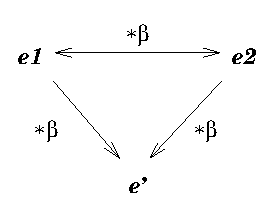
\includegraphics[scale=0.7]{church-rosser.eps}
      }
    \caption{Die Church/Rosser-Eigenschaft}
    \label{fig:church-rosser}
  \end{center}
\end{figure}

Eine wichtige Eigenschaft auf dem Weg zur Eindeutigkeit von
Normalformen ist der Satz von Church/Rosser:
%
\begin{satz}[Church/Rosser-Eigenschaft]\index{Church/Rosser-Eigenschaft}
  \label{satz:church-rosser}
  Die $\beta$-Reduktionsregel hat die 
  \textit{Church/Rosser"=Eigenschaft}:  Für
  beliebige $\lambda$-Terme $e_1$ und  $e_2$ mit
  $e_1 \overset{\ast}{\leftrightarrow_\beta} e_2$,
  gibt es immer einen $\lambda$-Term $e'$ mit
  $e_1\overset{\ast}{\rightarrow_\beta} e'$ und
  $e_2\overset{\ast}{\rightarrow_\beta} e'$.
\end{satz}
%
Abbildung~\ref{fig:church-rosser} stellt die Aussage des Satzes von
Church/Rosser grafisch dar.
Der Beweis des Satzes ist leider recht umfangreich und technisch.
Die einschlägige Literatur über den $\lambda$-Kalkül hat ihn
vorrätig~\cite{HindleySeldin1986}.

Die Church/Rosser-Eigenschaft ebnet den Weg für Benutzung von
Normalformen zum Finden von Beweisen im $\lambda$-Kalkül:
%
\begin{satz}[Eindeutigkeit der Normalform]
  \label{satz:normalform}
  Ein $\lambda$-Term $e$ hat höchstens eine Normalform modulo
  $\alpha$-Reduktion.
\end{satz}
%
  \begin{beweis}
    Angenommen, es gebe zwei unterschiedliche Normalformen $e_1$ und
    $e_2$ von $e$.  Nach Satz~\ref{satz:church-rosser} muß es dann
    aber einen weiteren $\lambda$-Term $e'$ geben mit   $e_1\overset{\ast}{\rightarrow_\beta} e'$ und
  $e_2\overset{\ast}{\rightarrow_\beta} e'$.  Entweder sind $e_1$ und
    $e_2$ also nicht unterschiedlich, oder zumindest einer von
    beiden ist keine Normalform im Widerspruch zur Annahme.
  \end{beweis}
%
  Satz~\ref{satz:normalform} bestätigt, daß
  der $\lambda$-Kalkül ein sinnvoller Mechanismus für die Beschreibung
  des Verhaltens von Computerprogrammen ist: Bei einem $\lambda$-Term
  ist es gleichgültig, in welcher Reihenfolge die Reduktionen
  angewendet werden: Jede Reduktionsfolge, die zu einer Normalform
  führt, führt immer zur gleichen Normalform.

\section{Der $\lambda$-Kalkül als Programmiersprache}
\label{sec:lambdaprog}

Mit dem Normalformsatz ist geklärt, daß Terme im
$\lambda$-Kalkül, die eine Normalform besitzen, so etwas wie einen
"<Sinn"> haben, der unabhängig von der Reihenfolge der
Reduktionsschritte ist.  Bleibt die Frage, ob der $\lambda$-Kalkül
"<groß genug"> ist, um Computerprogramme abzubilden.

Auf den ersten Blick erscheint das etwas unwahrscheinlich: In der Welt
des $\lambda$-Kalküls gibt es direkt
keine eingebauten booleschen Werte oder Zahlen.
Diese lassen sich jedoch durch Funktionen nachbilden.  Das heißt,
daß der $\lambda$-Kalkül ebenso mächtig wie eine ausgewachsene
Programmiersprache ist.  Dadurch, daß er aber nur eine zentrale
Reduktionsregel besitzt, eignet er sich aber viel besser als eine
komplizierte Programmiersprache für die formale Manipulation.

Dieser Abschnitt zeigt, wie sich die wichtigsten Elemente einer
Programmiersprache im Kalkül nachbilden lassen:
%
\begin{itemize}
\item Verzweigungen und boolesche Werte
\item Zahlen
\item Rekursion
\end{itemize}
%
\subsection{Verzweigungen}
\label{sec:booleans}
%
Verzweigungen haben ihre primäre Daseinsberechtigung in Verbindung mit
booleschen Werten\index{boolescher Wert} und umgekehrt.
Die binäre Verzweigung\index{Verzweigung} in den Lehrsprachen
\texttt{(if \(t\) \(k\) \(a\))}
wählt, abhängig vom Wert von $t$,
entweder die Konsequente $k$ oder die Alternative $a$ aus.  Die Nachbildung im
$\lambda$-Kalkül stellt dieses Prinzip auf den Kopf: die Maschinerie
für die Auswahl zwischen Konsequente und Alternative wird in die
booleschen Werte selbst gesteckt.  $\mathit{true}$\index{true@$\mathit{true}$} ist ein
$\lambda$-Term, der das erste von zwei Argumenten auswählt und das
zweite verwirft; $\mathit{false}$\index{false@$\mathit{false}$} selektiert das zweite und verwirft
das erste:
%
\begin{align*}
  \mathit{true} & \deq{} \lambda x y.x \\
  \mathit{false} & \deq{} \lambda x y.y
\end{align*}
%
Damit hat die Verzweigung selbst nicht mehr viel zu tun; sie wendet
einfach den Test, der einen booleschen Wert ergeben muß, auf
Konsequente und Alternative an:
%
\begin{displaymath}
  \mathit{if} \deq{} \lambda t x y.t~x~y
\end{displaymath}
%
Daß $\mathit{if}$\index{if@$\mathit{if}$} tatsächlich so funktioniert wie angenommen, läßt
sich an einem Beispiel leicht sehen:
%
\begin{displaymath}
  \begin{split}
    \mathit{if}~\mathit{true}~e_1~e_2 & =
    (\lambda t x y.t~x~y)~\mathit{true}~e_1~e_2
    \\
    & \rightarrow_\beta (\lambda x y.\mathit{true}~x~y)~e_1~e_2\\
    & \rightarrow_\beta^2 \mathit{true}~e_1~e_2\\
    & = (\lambda x y.x)~e_1~e_2\\
    & \rightarrow_\beta (\lambda y.e_1)~e_2\\
    & \rightarrow_\beta e_1  \end{split}
\end{displaymath}
%
Für $\mathit{false}$ geht der Beweis analog.

\subsection{Natürliche Zahlen}

Die Nachbildung von Zahlen ist etwas komplizierter als die der
booleschen Werte.  Eine Methode dafür ist
die Verwendung von \textit{Church-Numeralen\index{Church-Numeral}}.  Das
Church-Numeral $\lceil n\rceil$ einer natürlichen Zahl\index{natürliche Zahl}
$n$ ist eine Funktion, die eine $n$-fache Applikation vornimmt.
%
\begin{displaymath}
  \lceil n\rceil \deq{} \lambda f\lambda x.f^n(x)
\end{displaymath}
Für einen $\lambda$-Term $f$ ist $f^n : \mathcal{L}_{\lambda}\rightarrow\mathcal{L}_{\lambda}$ folgendermaßen induktiv definiert:
%
\begin{displaymath}
  f^n(e) \deq
  \begin{cases}
    e & \text{falls } n = 0\\
    f(f^{n-1}(e)) & \text{sonst}
  \end{cases}
\end{displaymath}
%
$\lceil 0\rceil$\index{*@$\lceil \:\rceil$} ist nach dieser Definition
$\lambda f.\lambda x.x$, $\lceil 1\rceil$ ist $\lambda f.\lambda x.f~x$,
$\lceil 2\rceil$ ist $\lambda f.\lambda x.f(f~x)$, usw.

Die Nachfolgeroperation\index{Nachfolger} hängt eine zusätzliche Applikation an:\index{succ@$\mathit{succ}$}
%
\begin{displaymath}
  \mathit{succ} \deq{} \lambda n.\lambda f.\lambda x.n~f~(f~x)
\end{displaymath}
%
Der folgende Term bildet die Vorgängerfunktion ab\index{Vorgänger}\index{pred@$\mathit{pred}$}:
%
\begin{displaymath}
  \mathit{pred} \deq{} \lambda x.\lambda y.\lambda z.x~(\lambda p.\lambda
  q.q~(p~y))~((\lambda x.\lambda y.x)~z)~(\lambda x.x)
\end{displaymath}
%
Der Beweis dafür, daß sich $\mathit{pred}$ in bezug auf $\mathit{succ}$ wie die
Vorgängerfunktion verhält, ist Übungsaufgabe~\ref{ex:pred}.

In Verbindung mit den booleschen Werten läßt sich eine Zahl daraufhin
testen, ob sie $0$ ist:\index{zerop@$\mathit{zerop}$}
%
\begin{displaymath}
  \mathit{zerop} \deq{} \lambda n.n~(\lambda x.\mathit{false})~\mathit{true}
\end{displaymath}
%
Die Funktionsweise von $\mathit{zerop}$ läßt sich am einfachsten an
einem Beispiel erkennen:
%
\begin{displaymath}
  \begin{split}
    \mathit{zerop}~\lceil 0\rceil & =
    (\lambda n.n~(\lambda x.\mathit{false})~\mathit{true})~\lceil 0\rceil\\
    & \rightarrow_\beta \lceil 0\rceil~(\lambda x.\mathit{false})~\mathit{true}\\
    & = (\lambda f.\lambda x.x)~(\lambda x.\mathit{false})~\mathit{true}\\
    & \rightarrow_\beta (\lambda x.x)~\mathit{true}\\
    & \rightarrow_\beta \mathit{true}
  \end{split}
\end{displaymath}
%

\subsection{Rekursion und Fixpunktsatz}
%
Schließlich fehlt noch die Rekursion\index{Rekursion}.  Das Hauptproblem dabei ist, daß
es im $\lambda$-Kalkül kein Pendant zu \texttt{define} oder
\texttt{letrec} gibt: Es gibt keine direkte Möglichkeit, eine
rekursive Bindung herzustellen.  Zur Realisierung von Rekursion ist
deshalb ein Kunstgriff notwendig, der sich an der rekursiven
Definition der Fakultät zeigen läßt.
Schön wäre eine Definition wie folgt, wobei Zahlen ohne $\lceil\:\rceil$ für
ihre Church-Numerale stehen:\index{fac@$\mathit{fac}$}
%
\begin{displaymath}
  \mathit{fac} \deq{} \lambda x.\mathit{if}~(\mathit{zerop}~x)~1~(\ast~x~(\mathit{fac}~(\mathit{pred}~x)))
\end{displaymath}
%
$=$ und $\ast$ stehen dabei für $\lambda$-Terme, die Church-Numerale
vergleichen bzw.\ multiplizieren.  (Ihre Formulierung ist Teil der
Übungsaufgabe~\ref{ex:church}.)

Leider ist diese Formulierung von $\mathit{fac}$ keine richtige
Definition: $\mathit{fac}$ taucht sowohl auf der linken
als auch auf der rechten Seite auf.  Wenn $\mathit{fac}$ aus der
rechten Seite entfernt wird, bleibt folgender Term übrig:
%
\begin{displaymath}
  \lambda x.\mathit{if}~(\mathit{zerop}~x~1)~1~(\ast~x~(?~(\mathit{pred}~x)))
\end{displaymath}
%
Immerhin ist zu sehen, daß dieser Term korrekt die Fakultät von $0$
ausrechnet, nämlich $1$.  Für alle Zahlen größer als $0$ ist es allerdings
schlecht bestellt, da der Term "<$?$"> noch unbekannt ist.
Weil der obige Term nur für $0$ taugt, sei er mit $\mathit{fac}_0$
benannt:
%
\begin{displaymath}
  \mathit{fac}_0 \deq \lambda x.\mathit{if}~(\mathit{zerop}~x)~1~(\ast~x~(?~(\mathit{pred}~x)))
\end{displaymath}
%
Nun wäre es schön, einen Term zu haben, der zumindest auch die
Fakultät von $1$ ausrechnen kann.  Dazu wird $\mathit{fac}_0$ in
seine eigene Definition anstelle des $?$ eingesetzt.  Das Ergebnis
sieht so aus:
%
\begin{displaymath}
  \lambda x.\mathit{if}~(\mathit{zerop}~x)~1~(\ast~x~(\mathit{fac}_0~(\mathit{pred}~x)))
\end{displaymath}
%
Da $\mathit{fac}_0$ keinen Selbstbezug enthält, läßt sich seine
Definition einsetzen; das Ergebnis soll der Funktion entsprechend
$\mathit{fac}_1$ heißen:
%
\begin{displaymath}
  \mathit{fac}_1 \deq{} \lambda x.\mathit{if}~(\mathit{zerop}~x)~1~(\ast~x~((\lambda x.\mathit{if}~(\mathit{zerop}~x)~1~(\ast~x~(?~(\mathit{pred}~x))))~(\mathit{pred}~x)))
\end{displaymath}
%
Auf die gleiche Art und Weise läßt sich ein Term konstruieren, der
alle Fakultäten bis 2 ausrechnen kann:
%
\begin{displaymath}
  \mathit{fac}_2 \deq{} \lambda x.\mathit{if}~(\mathit{zerop}~x)~1~(\ast~x~(\mathit{fac}_1~(\mathit{pred}~x)))
\end{displaymath}
%
Dieses Muster läßt sich immer so weiter fortsetzen.  Leider entsteht
dabei trotzdem nie ein Term, der die Fakultäten \emph{aller}
natürlichen Zahlen berechnen kann, da die Terme immer endlich groß
bleiben.

Immerhin aber enthalten alle $\mathit{fac}_n$-Terme das
gleiche Muster und unterscheiden sich nur durch Aufruf von
$\mathit{fac}_{n-1}$.  Also ist es sinnvoll, Abstraktion
das Problem anzuwenden:
%
\begin{displaymath}
  \lambda\mathit{fac}.\lambda x.\mathit{if}~(\mathit{zerop}~x)~1~(\ast~x~(\mathit{fac}~(\mathit{pred}~x)))
\end{displaymath}
%
Dieser Term soll $\mathit{FAC}$\index{FAC@$\mathit{FAC}$} heißen.  Nun lassen sich die
$\mathit{fac}_n$-Funktionen mit Hilfe von $\mathit{FAC}$ einfacher beschreiben:
%
\begin{eqnarray*}
   \mathit{fac}_0 &\deq{}& \lambda x.\mathit{if}~(\mathit{zerop}~x)~1~(\ast~x~(?~(\mathit{pred}~x)))\\
   \mathit{fac}_1 &\deq{}& \mathit{FAC}~\mathit{fac}_0\\
   \mathit{fac}_2 &\deq{}& \mathit{FAC}~\mathit{fac}_1\\
   \mathit{fac}_3 &\deq{}& \mathit{FAC}~\mathit{fac}_2\\
   &\ldots&
\end{eqnarray*}
%
$\mathit{FAC}$ ist also eine Fabrik für Fakultätsfunktionen und
teilt mit allen $\mathit{fac}_i$ die Eigenschaft, daß ihre
Definition nicht rekursiv ist.

Damit ist zwar die Notation weniger schreibintensiv geworden,
aber das fundamentale Problem ist noch nicht gelöst: Eine korrekte
Definition von $\mathit{fac}$ müßte eine unendliche
Kette von Applikationen von $\mathit{FAC}$ enthalten.
Da sich ein Term mit einer unendlichen Kette von Applikationen nicht aufschreiben läßt, hilft im Moment nur Wunschdenken weiter.
Dafür sei angenommen, $\mathit{fac}$ wäre bereits gefunden.  Dann gilt folgende
Gleichung:
%
\begin{displaymath}
  \mathit{fac} \equiv \mathit{FAC}~\mathit{fac}
\end{displaymath}

\begin{figure}[!tb]
  \begin{center}
    \scriptsize
    \begin{eqnarray*}
    \mathit{fac}~3 &=& Y~\mathit{FAC}~3\\
    \text{(Satz~\ref{satz:fixpunkt})} &\overset{\ast}{\rightarrow_{\beta}}&
    \mathit{FAC}~(Y~\mathit{FAC})~3\\
    &\rightarrow_{\beta}&
    (\lambda x.\mathit{if}~(\mathit{zerop}~x)~1~(\ast~x~((Y~\mathit{FAC})~(\mathit{pred}~x))))~3\\
    &\rightarrow_{\beta}&
    \mathit{if}~(\mathit{zerop}~ 3)~1~(\ast~3~((Y~\mathit{FAC})~(\mathit{pred}~3)))
    \\
    &\overset{\ast}{\rightarrow_{\beta}}&
    \mathit{if}~\mathit{false}~1~(\ast~3~((Y~\mathit{FAC})~2))\\
    &\overset{\ast}{\rightarrow_{\beta}}&
    \ast~3~((Y~\mathit{FAC})~2)\\
    \text{(Satz~\ref{satz:fixpunkt})} &\overset{\ast}{\rightarrow_{\beta}}&
    \ast~3~(\mathit{FAC}~(Y~\mathit{FAC})~2)\\
    &\rightarrow_{\beta}&
    \ast~3~((\lambda
    x.\mathit{if}~(\mathit{zerop}~x)~1~(\ast~x~((Y~\mathit{FAC})~(\mathit{pred}~x))))~2)\\
    &\rightarrow_{\beta}&
    \ast~3~(\mathit{if}~(\mathit{zerop}~ 2)~1~(\ast~2~((Y~\mathit{FAC})~(\mathit{pred}~2))))\\
    &\overset{\ast}{\rightarrow_{\beta}}&
    \ast~3~(\mathit{if}~\mathit{false}~1~(\ast~2~((Y~\mathit{FAC})~1)))\\
    &\overset{\ast}{\rightarrow_{\beta}}&
    \ast~3~(\ast~2~((Y~\mathit{FAC})~1))\\
    \text{(Satz~\ref{satz:fixpunkt})} &\overset{\ast}{\rightarrow_{\beta}}&
    \ast~3~(\ast~2~(\mathit{FAC}~(Y~\mathit{FAC})~1))\\
    &\rightarrow_{\beta}&
    \ast~3~(\ast~2~((\lambda
    x.\mathit{if}~(\mathit{zerop}~x)~1~(\ast~x~((Y~\mathit{FAC})~(\mathit{pred}~x))))~1))\\
%
%
    &\rightarrow_{\beta}&
    \ast~3~(\ast~2~(\mathit{if}~(\mathit{zerop}~1)~1~(\ast~1~((Y~\mathit{FAC})~(\mathit{pred}~1)))))\\
    &\overset{\ast}{\rightarrow_{\beta}}&
    \ast~3~(\ast~2~(\mathit{if}~\mathit{false}~1~(\ast~1~((Y~\mathit{FAC})~0))))\\
    &\overset{\ast}{\rightarrow_{\beta}}&
    \ast~3~(\ast~2~(\ast~1~((Y~\mathit{FAC})~0)))\\
    \text{(Satz~\ref{satz:fixpunkt})} &\overset{\ast}{\rightarrow_{\beta}}&
    \ast~3~(\ast~2~(\ast~1~(\mathit{FAC}~(Y~\mathit{FAC})~0)))\\
    &\rightarrow_{\beta}&
    \ast~3~(\ast~2~(\ast~1~((\lambda
    x.\mathit{if}~(\mathit{zerop}~x)~1~(\ast~x~((Y~\mathit{FAC})~(\mathit{pred}~x))))~0)))\\
%
%
    &\rightarrow_{\beta}&
    \ast~3~(\ast~2~(\ast~1~(\mathit{if}~(\mathit{zerop}~0)~1~(\ast~1~((Y~\mathit{FAC})~(\mathit{pred}~0))))))\\
    &\overset{\ast}{\rightarrow_{\beta}}&
    \ast~3~(\ast~2~(\ast~1~(\mathit{if}~\mathit{true}~1~(\ast~1~((Y~\mathit{FAC})~(\mathit{pred}~0))))))\\
    &\overset{\ast}{\rightarrow_{\beta}}&
    \ast~3~(\ast~2~(\ast~1~1))\\
    &\overset{\ast}{\rightarrow_{\beta}}&
    6
    \end{eqnarray*}
    \caption{Berechnung der Fakultät von 3 im $\lambda$-Kalkül}
    \label{fig:fac3}
  \end{center}
\end{figure}

Die eine zusätzliche Applikation, die $\mathit{FAC}$ vornimmt, landet
auf einem ohnehin schon unendlichen Stapel,
macht diesen also auch nicht größer.  Damit ist aber $\mathit{fac}$ ein sogenannter
\textit{Fixpunkt\index{Fixpunkt}} von $\mathit{FAC}$:  Wenn $\mathit{fac}$
hineingeht, kommt es auch genauso wieder heraus.  Wenn es nun eine
Möglichkeit gäbe, für einen $\lambda$-Term einen Fixpunkt zu finden,
wäre das Problem gelöst.  Der folgende Satz zeigt, daß dies tatsächlich
möglich ist:
%
\begin{satz}[Fixpunktsatz]\index{Fixpunktsatz}
  \label{satz:fixpunkt}
  Für jeden $\lambda$-Term $F$ gibt es einen $\lambda$-Term $X$ mit
  $F~X\equiv X$.
\end{satz}
\begin{beweis}
  Wähle $X \deq{} Y~F$, wobei
  %
  \begin{displaymath}
    Y \deq{} \lambda f.(\lambda x.f~(x~x))~(\lambda x.f~(x~x)).
  \end{displaymath}
  %
  Dann gilt:
  %
  \begin{displaymath}
    \begin{split}
      Y~F & = (\lambda f.(\lambda x.f~(x~x))~(\lambda x.f~(x~x)))~F
      \\ & \rightarrow_\beta
      (\lambda x.F~(x~x))~(\lambda x.F~(x~x))
      \\ & \rightarrow_\beta
      F~((\lambda x.F~(x~x))~(\lambda x.F~(x~x)))
      \\ & \leftarrow_\beta
      F~((\lambda f.(\lambda x.f~(x~x))~(\lambda x.f~(x~x)))~F)
      \\ & =
      F~(Y~F)
    \end{split}
  \end{displaymath}
\end{beweis}
%
Der $\lambda$-Term $Y$\index{Y@$Y$}, der Fixpunkte
berechnet, heißt
\textit{Fixpunktkombinator\index{Fixpunktkombinator}}.  Mit seiner Hilfe läßt sich
die Fakultät definieren:
%
\begin{displaymath}
  \mathit{fac} \deq{} Y~\mathit{FAC}
\end{displaymath}
%

Abbildung~\ref{fig:fac3} zeigt, wie die Berechnung der Fakultät von
$3$ mit dieser Definition funktioniert.

\section{Auswertungsstrategien}
\label{sec:lambda-evaluation-strategies}

\index{Auswertungsstrategie}Die Definitionen des vorangegangenen Abschnitts zusammen mit dem Satz
von Church/\linebreak[0]Rosser sind wichtige Meilensteine auf dem Weg zur
Verwendung des $\lambda$-Kalküls als Basis für reale
Programmiersprachen.  Leider hat die Anwendung des Satzes von
Church/Rosser noch einen Haken in der Praxis: Er besagt zwar, daß sich
die Äquivalenz von zwei Termen dadurch beweisen läßt, daß ihre
Normalformen verglichen werden.  Leider sagt er nichts darüber,
wie diese Normalformen gefunden werden.

Zum systematischen Finden von Normalformen gehört
eine \textit{Auswertungsstrategie}.  Eine
solche Strategie ist dafür zuständig, von den $\beta$-Redexen
innerhalb eines $\lambda$-Terms denjenigen auszusuchen, der
tatsächlich reduziert wird.  Für den $\lambda$-Kalkül gibt es mehrere
populäre Auswertungsstrategien, die jeweils ihre eigenen Vor- und
Nachteile haben, was das effektive Finden von Normalformen betrifft.

Eine populäre Auswertungsstrategie ist die Linksaußen-Reduktion\index{Linksaußen-Reduktion}, auch
\textit{normal-order reduction\index{normal-order reduction}} oder
\textit{leftmost-outermost reduction\index{leftmost-outermost reduction}} genannt:
%
\begin{definition}[Linksaußen-Reduktion]
  Die Relation $\rightarrow_{\beta o}$, die
  \textit{Linksaußen-Reduktion}, ist durch die gleiche Regel wie
  die $\beta$-Reduktion definiert:
  %
  \begin{displaymath}
    (\lambda v.e)~f \rightarrow_{\beta o} e[v\mapsto f]
  \end{displaymath}
  %
  Diese Regel darf nur auf bestimmte Subterme angewendet werden,
  nämlich solche $\beta$-Redexe, die möglichst weit
  links außen stehen.
\end{definition}
%
Die Linksaußen-Reduktion hat folgende äußerst angenehme Eigenschaft:
%
\begin{satz}
  Wenn $e'$ eine Normalform von $e$ ist, so gilt
  $e\overset{\ast}{\rightarrow_{\beta o}} e'$.
\end{satz}
%
Falls es also eine Normalform gibt, so findet die Linksaußen-Reduktion
sie auch.

Es gibt allerdings noch weitere Auswertungsstrategien.  Die sogenannte
Call-by-Name-Auswertung basiert auf dem Konzept der \textit{schwachen
  Kopfnormalform\index{schwache Kopfnormalform}\index{Kopfnormalform!schwach}}:

\begin{definition}[Schwache Kopfnormalform]\label{def:wert}
  Unter den $\lambda$"=Termen heißen die Abstraktionen auch
  \textit{Werte} oder \textit{schwache Kopfnormalformen}.  Ein
  $\lambda$-Term, der kein Wert\index{Wert} ist, heißt \textit{Nichtwert\index{Nichtwert}}.  %In
%  Grammatiken werden Werte durch das Nichtterminal \meta{value}
%  bezeichnet:
%  \begin{grammar}
%      \meta{value} \: $($ $\lambda$ \meta{var}.\meta{exp} $)$
%  \end{grammar}
\end{definition}

\begin{definition}[Call-by-Name-Auswertung]
  Die Relation $\rightarrow_{\beta n}$, die
  \textit{Call"=by"=Name"=Reduktion}, ist durch folgende Regel
  definiert,
  die wiederum identisch zur normalen Regel für $\beta$-Reduktion ist:
  %
  \begin{displaymath}
    (\lambda v.e)~f \rightarrow_{\beta n} e[v\mapsto f]
  \end{displaymath}
  %
  Diese Regel darf nur in einem Gesamtterm angewendet werden,
  wenn dieser noch nicht in schwacher Kopfnormalform ist, und auch dann
  nur auf Subterme, die $\beta$-Redexe sind, die möglichst weit
  links außen stehen.
\end{definition}
%
Die Call-by-Name-Auswertung ist damit ähnlich zur
Linksaußen"=Auswertung, aber nicht ganz so aggressiv: sie gibt sich
schon mit einer schwachen Kopfnormalform zufrieden anstatt einer
"<richtigen"> Normalform.  Dies ist bei der Verwendung als
Auswertungsstrategie in Programmiersprachen allerdings schon
genug: die weitere Auswertung des Rumpfes einer schwachen
Kopfnormalform wird einfach verschoben auf die Zeit der Applikation.

Linksaußen- und Call-by-Name-Auswertung finden zwar immer eine
Normalform bzw.\ eine schwache Kopfnormalform, wenn es eine solche
gibt; gelegentlich aber geschieht dies nicht auf die effektivste Art
und Weise.  Im folgendem Term wird bei Linksaußen- und
Call-by-Name-Reduktion zuerst der äußere Redex reduziert:
%
\begin{displaymath}
  \begin{array}{rl}
  (\lambda x.x~x)~((\lambda y.y)~z)
  \rightarrow_{\beta o} & 
  ((\lambda y.y)~z)~((\lambda y.y)~z)
  \\
  \rightarrow_{\beta o} & 
  z~((\lambda y.y)~z)
  \\
  \rightarrow_{\beta o} & 
  z~z
\end{array}
\end{displaymath}
%
Bei dieser Reduktionsfolge wurde der Subterm $((\lambda y.y)~z)$
zunächst "<verdoppelt"> und mußte demnach auch zweimal reduziert
werden.  Eine andere Auswertungsstrategie verspricht die Vermeidung
solcher doppelter Arbeit:  Die meisten Programmiersprachen verwenden
eine Strategie, die von der sogenannten \textit{Linksinnen-Reduktion},
auch genannt \emph{applicative-order reduction\index{applicative-order reduction}} oder
\emph{leftmost-innermost reduction\index{leftmost-innermost reduction}} abgeleitet ist:
%
\begin{definition}[Linksinnen-Reduktion]\index{Linksinnen-Reduktion}
  In dieser Definition steht $w$ immmer für einen Wert.
  Die Relation $\rightarrow_{\beta i}$, die
  \textit{Linksinnen"=Reduktion}, ist definiert durch die
  folgende Regel:
  %
  \begin{displaymath}
    (\lambda v.e)~w \rightarrow_{\beta i} e[v \mapsto w].
  \end{displaymath}
  %
  $\rightarrow_{\beta i}$ ist dabei nur anwendbar auf Subterme, die
  möglichst weit links innen stehen.
\end{definition}
%
Die Linksinnen-Reduktion ist beim obigen Beispiel effektiver, da
zunächst das Argument der äußeren Applikation ausgewertet wird:
%
\begin{displaymath}
  \begin{array}{rl}
  (\lambda x.x~x)~((\lambda y.y)~(\lambda z.z))
  \rightarrow_{\beta i} & 
  (\lambda x.x~x)~(\lambda z.z)
  \\
  \rightarrow_{\beta i} & 
  (\lambda z.z)~(\lambda z.z)
  \\
  \rightarrow_{\beta i} & 
  (\lambda z.z)
\end{array}
\end{displaymath}
%
Leider führt die Linksinnen-Reduktion nicht immer zu einer Normalform,
selbst wenn es die Linksaußen-Reduktion tut.  Der Term
\[ (\lambda x.\lambda y.y)~((\lambda z.z~z)~(\lambda z.z~z)) \]
zum Beispiel hat zwei Redexe, einmal den ganzen Term und dann noch
\[(\lambda z.z~z)~(\lambda z.z~z).\]  Die Linksinnen-Strategie wählt
den inneren Subterm als ersten Redex aus:
%
\begin{displaymath}
  (\lambda z.z~z)~(\lambda z.z~z)
\rightarrow_{\beta i}
  (\lambda z.z~z)~(\lambda z.z~z).
\end{displaymath}
%
Damit läuft die Linksinnen-Reduktion unendlich im Kreis, während
die Linksaußen"=Reduktion sofort den gesamten Term reduziert und die
Normalform $\lambda y.y$ liefert.

Eine Ableitung der Linksinnen-Reduktion, die in den meisten
Programmiersprachen Anwendung findet, ist die
\textit{Call-by-Value-Reduktion\index{Call-by-Value-Reduktion}}:
%
\begin{definition}[Call-by-Value-Reduktion]\label{def:call-by-value}
  In dieser Definition steht $w$ immmer für einen Wert und $e$ für
  einen Nichtwert.  Die Relation $\rightarrow_{\beta v}$, die
  \textit{Call"=by"=Value"=Reduktion}, ist definiert durch die
  folgende Regel:
  %
  \begin{displaymath}
    (\lambda v.e)~w \rightarrow_{\beta v} e[v \mapsto w].
  \end{displaymath}
  %
  $\rightarrow_{\beta v}$ darf nur in einem Gesamtterm angewendet
  werden, wenn dieser keine schwache Kopfnormalform ist,
  und dann nur auf einen Subterm, der möglichst weit links innen steht.
\end{definition}

\section{Die Auswertungsstrategie der Lehrsprachen}
\label{sec:scheme-auswertung}

Mit der Call-by-Value-Reduktion ist die Grundlage für die
Auswertungsstrategie der Lehrsprachen gelegt.  Tatsächlich definiert das
Substitutionsmodell eine Variante der
Call-by-Value-Auswertung.  Zur Erinnerung ist hier noch einmal die
Definition der wichtigsten Regel des Substitutionsmodells, nämlich der für
Funktionanwendungen der Form \texttt{(\(p\) \(o\sb{1}\) \(\ldots\) \(o\sb{n}\))}:
%
\begin{quote}
  [\ldots] Zunächst werden Operator $p$ und Operanden $o_1, \ldots, o_n$
  ausgewertet.  Der Wert von $p$ muß eine Funktion sein. [\ldots]
\end{quote}
%
Der entscheidende Satz ist dabei der letzte:
Er bedeutet, daß innen zuerst ausgewertet wird;
treten bei der Auswertung von Operator und Operanden weitere
Funktionanwendungen auf, wird das gleiche Prinzip rekursiv angewendet.
Damit ist das Substitutionsmodell eng verwandt mit der
Call-by-Value-Auswertung im Lambda-Kalkül.

Programmiersprachen, die von innen nach außen auswerten, heißen
\textit{Call-by-Value-Sprachen\index{Call-by-Value-Sprache}} oder
\textit{strikten\index{strikte Sprache} Sprachen} zu sprechen.  Neben
den Lehrsprachen gehören auch OCaml, Clojure, Scala, Erlang, Elixir,
C, Java, Pascal und ML und viele andere zu den strikten Sprachen.

Es gibt auch \textit{nicht-strikte\index{nicht-strikte Sprache}}
Sprachen wie z.B.\ Haskell,
die auf der sogenannten \textit{lazy evaluation\index{lazy evaluation}} beruhen.  Ihre
Auswertungsstrategie ist eng mit der Call-by-Name-Auswertung im
$\lambda$-Kalkül verwandt.  Allerdings vermeiden diese Sprachen die
mehrfache überflüssige Auswertung von Ausdrücken dadurch, daß sie den
Wert beim ersten Mal abspeichern und danach wiederverwenden.

\section*{Übungsaufgaben}
\begin{aufgabe}\label{ex:pred}
  Beweise, daß $\mathit{pred}$ den Vorgänger eines
  positiven Church-Numerals berechnet!
\end{aufgabe}

\begin{aufgabe}\label{ex:church}
  Beweise, daß es Lambda-Terme für die folgenden arithmetischen
  Operationen auf Church-Numeralen gibt:
  %
  \begin{eqnarray*}
    \mathit{add} \lceil m\rceil \lceil n\rceil &=& \lceil m+n\rceil
    \\
    \mathit{mult} \lceil m\rceil \lceil n\rceil &=& \lceil mn\rceil
    \\
    \mathit{exp} \lceil m\rceil \lceil n\rceil &=& \lceil m^n\rceil
    \textrm{ für } m>0\\
    \mathit{=}\lceil m\rceil \lceil n\rceil &=&
    \begin{cases}
      \mathit{true} & \text{falls } m = n\\
      \mathit{false} & \text{sonst}
    \end{cases}
  \end{eqnarray*}
  %
  Benutze dazu die folgenden Definitionen:
  \begin{eqnarray*}
    \mathit{add} &\deq{}& \lambda x.\lambda y.\lambda p.\lambda q.xp(ypq)\\
    \mathit{mult} &\deq{}& \lambda x.\lambda y.\lambda z.x(yz)\\
    \mathit{exp} &\deq{}& \lambda x.\lambda y.y x
  \end{eqnarray*}
  und gibt eine eigene Definition für $=$ an.
  %
  Dabei läßt sich die Korrektheit von $\mathit{add}$ direkt beweisen.
  Für $\mathit{mult}$ und $\mathit{exp}$ beweise und benutze dazu
  folgende Hilfslemmata:
  %
  \begin{displaymath}
    (\lceil n\rceil x)^m y \leftrightarrow_{\beta} x^{nm} y
  \end{displaymath}
  \begin{displaymath}
    \label{eq:lem-2}
    \lceil n\rceil^m x \leftrightarrow_{\beta} \lceil n^m\rceil
    \textrm{ für } m>0
  \end{displaymath}
\end{aufgabe}
\begin{aufgabe}
  Der Y-Kombinator ließe sich auch programmieren
  als:
 %
\begin{verbatim}
(define y 
  (lambda (f)
    ((lambda (x) (f (x x)))
     (lambda (x) (f (x x))))))
\end{verbatim}
  %
  Zeige durch Ausprobieren, daß \texttt{y} mit dieser Definition 
  nicht funktioniert.  Warum ist das so?  Benutze für die
  Erklärung das Substitutionsmodell!
  Zeige, daß die folgende Variante von \texttt{y} ein
  Fixpunktkombinator ist, der funktioniert:
  %
\begin{verbatim}
(define y
  (lambda (f)
    ((lambda (x)
       (f (lambda (y) ((x x) y))))
     (lambda (x)
       (f (lambda (y) ((x x) y)))))))
\end{verbatim}

\end{aufgabe}
\begin{aufgabe} (Quelle: Ralf Hinze, Bonn)
  Zeige, daß $F$ mit der folgenden Definition ebenfalls ein
  Fixpunktkombinator ist:
  \begin{eqnarray*}
    F &\deq{}& G^{[26]}
    \\
    G &\deq{}& \lambda abcdefghijklmnopqstuvwxyzr.r(dasisteinfixpunktkombinator)
  \end{eqnarray*}
  %
  Dabei steht $G^{[26]}$ für den Lambda-Term, der durch 26faches
  Hintereinanderschreiben von $G$ entsteht, also $GG\ldots G = (\ldots
  ((G G) G)\ldots G)$.
  

\end{aufgabe}

%%% Local Variables: 
%%% mode: latex
%%% TeX-master: "i1"
%%% End: 


% Diese Datei ist Teil des Buchs "Schreibe Dein Programm!"
% Das Buch ist lizensiert unter der Creative-Commons-Lizenz
% "Namensnennung 4.0 International (CC BY 4.0)"
% http://creativecommons.org/licenses/by/4.0/deed.de

\chapter{Die SECD-Maschine}\label{cha:secd}

Der $\lambda$-Kalkül ist als theoretisches Modell für berechenbare
Funktionen lange vor der Erfindung des Computers entwickelt worden.
Die Reduktionsregeln dienen dabei der Entwicklung von Beweisen über
die Äquivalenz von $\lambda$-Termen.  Damit der $\lambda$-Kalkül auch
als Modell für die tatsächliche Ausführung von Programmen, auf dem
Computer geeignet ist, fehlen noch zwei Zutaten: die direkte
Definition von "`eingebauten"' Werten und Operationen wie Zahlen und
booleschen Werten sowie ein formales Auswertungsmodell.  Dieses
Kapitel stellt zunächst den \textit{angewandten $\lambda$-Kalkül} vor,
der den normalen $\lambda$-Kalkül um primitive Werte und Operationen
erweitert, und dann die \textit{SECD-Maschine}, ein klassisches
Auswertungsmodell für die Call-by-Value-Reduktion.  Angenehmerweise
läßt sich die SECD-Maschine auch als Programm implementieren,
was ebenfalls in diesem Kapitel geschieht.  Die SECD-Maschine
kennt keine Zuweisungen; es folgt darum noch die Darstellung der
\textit{SECDH-Maschine}, die auch einen \textit{Speicher} kennt und
damit Zuweisungen korrekt modelliert.

Ab diesem Kapitel wird die Sprachebene \texttt{Schreibe
  Dein Programm! - fortgeschritten} benötigt. 

\section{Der angewandte $\lambda$-Kalkül}

Abschnitt~\ref{sec:lambdaprog} zeigte bereits, daß sich auch boolesche
Werte und Zahlen im $\lambda$-Kalkül durch $\lambda$-Terme darstellen
lassen.  Das ist zwar aus theoretischer Sicht gut zu wissen, auf Dauer
aber etwas mühsam: Darum ist es sinnvoll, mit einer erweiterten
Version des $\lambda$-Kalküls zu arbeiten, die solche "`primitiven"'
Werte direkt kennt.  Abschnitt~\ref{sec:lambdaprog} hat gezeigt,
daß eine solche Erweiterung nur syntaktischer Zucker ist,
also die Ausdruckskraft des Kalküls nicht wirklich erhöht.  Alle
Erkenntnisse aus dem normalen $\lambda$-Kalkül bleiben also erhalten.

Ein solcher erweiterter $\lambda$-Kalkül heißt auch
\textit{angewandter $\lambda$-Kalkül}:

\begin{definition}[Sprache des angewandten $\lambda$-Kalküls
  $\mathcal{L}_{\lambda{}A}$]\index{angewandter $\lambda$-Kalkül}\label{def:lambda-angewandt}
  
  Sei $V$ eine abzählbare Menge von Variablen.  Sei $B$ eine Menge von
  \textit{Basiswerten\index{Basiswert}}.  Sei für eine natürliche
  Zahl $n$ und $i \in \{1, \ldots, n\}$ jeweils $\Sigma^i$ eine Menge
  von \textit{$i$-stelligen Primitiva\index{Primitivum}}~-- die Namen
  von "`eingebauten Operationen"'.  Jedem $F^i\in\Sigma^i$ ist eine
  $i$-stellige Funktion $F_B^i: B\times\ldots\times B \rightarrow
  B$~-- ihre \textit{Operation}~--
  zugordnet.  Die Sprache des angewandten $\lambda$"=Kalküls, die
  Menge der \textit{angewandten $\lambda$-Terme},
  $\mathcal{L}_{\lambda{}A}$\index{L@$\mathcal{L}_{\lambda{}A}$}, ist
  durch folgende Grammatik definiert:
  \begin{grammar}
    \meta{$\mathcal{L}_{\lambda{}A}$} \: \meta{$V$}
    \> \| (\meta{$\mathcal{L}_{\lambda{}A}$} \meta{$\mathcal{L}_{\lambda{}A}$})
    \> \| ($\lambda$\meta{$V$}.\meta{$\mathcal{L}_{\lambda{}A}$})
    \> \| \meta{$B$}
    \> \| (\meta{$\Sigma^1$}~\meta{$\mathcal{L}_{\lambda{}A}$})
    \> \| (\meta{$\Sigma^2$}~\meta{$\mathcal{L}_{\lambda{}A}$}~\meta{$\mathcal{L}_{\lambda{}A}$})
    \> \ldots
    \> \| (\meta{$\Sigma^n$}~\meta{$\mathcal{L}_{\lambda{}A}$}~\ldots~\meta{$\mathcal{L}_{\lambda{}A}$}) \quad \textrm{($n$-mal)}
  \end{grammar}
  Die Grammatik ist abgekürzt notiert: Die letzen Klauseln besagen,
  daß es für jede Stelligkeit $i$ eine Klausel mit \meta{$\Sigma^i$} gibt,
  bei der jeweils $i$ Wiederholungen von
  \meta{$\mathcal{L}_{\lambda{}A}$}~-- entsprechend der Stelligkeit
  der Primitiva in $\Sigma^i$.
  %
Dabei heißen Terme der Form $(F^k~e_1~\ldots~e_k)$ auch
\textit{primitive Applikationen\index{primitive Applikation}}.
\end{definition}
%
In diesem Kapitel dienen normalerweise die Zahlen als Basiswerte mit
den üblichen Operationen wie $+$, $-$, $\ast$, $/$ etc.  Damit sind
Terme wie zum Beispiel $(+~(-~5~3)~17)$ möglich.

Im angewandten $\lambda$-Kalkül kommen zu den Werten aus
Definition~\ref{def:wert} die Basiswerte dazu:
%
\begin{definition}[Werte im angewandten $\lambda$-Kalkül]\label{def:wert-angewandt}
  Im angewandten $\lambda$-Kalkül heißen die Abstraktionen und
  Basiswerte kollektiv \textit{Werte}.  Ein $\lambda$-Term, der kein
  Wert\index{Wert} ist, heißt \textit{Nichtwert\index{Nichtwert}}.
\end{definition}

Damit die primitiven Operationen auch tatsächlich eine Bedeutung
bekommen, muß eine spezielle Reduktionsregel für sie eingeführt
werden:
%
\begin{definition}[$\delta$-Reduktion]\index{delta-Reduktion@$\delta$-Reduktion}
\begin{displaymath}
  (F^k~e_1~\ldots~e_k) \rightarrow_{\delta} F_B^k(e_1, \ldots, e_k)
  \quad e_1, \ldots, e_k \in B
\end{displaymath}
\end{definition}
%
Diese Regel besagt, daß eine primitive Applikation, wenn alle
Operanden Werte sind, durch Anwendung der entsprechenden Operation 
reduziert werden kann.  Damit wird z.B.\ der
obige Beispielterm folgendermaßen reduziert:
%
\begin{displaymath}
  (+~(-~5~3)~17) \rightarrow_{\delta} (+~2~17) \rightarrow_{\delta} 19
\end{displaymath}

\section{Die einfache SECD-Maschine}

Wie schon in Abschnitt~\ref{sec:scheme-auswertung} erwähnt, ist 
der Call-by-Value-$\lambda$-Kalkül\index{Call-by-Value-Reduktion}
ein Modell für die Auswertung der Lehrsprachen und viele andere
Programmiersprachen .
Allerdings ist Definition~\ref{def:call-by-value} strenggenommen etwas
vage: Es wird immer nur der Subterm reduziert, der
"`möglichst weit links innen steht"', aber was das heißt, ist nicht
genau definiert.  Außerdem ist Reduktion zwar ein
mächtiges formales Modell, entspricht aber nicht der
Ausführungsmethode tatsächlicher Programmiersprachen auf echten
Prozessoren.  Ein präzises und echten Maschinen deutlich näheres
Modell ist die \textit{SECD-Maschine\index{SECD-Maschine}}, erfunden
schon in den 60er Jahren von Peter Landin~\cite{Landin1964}, und
seitdem die Grundlage für zahllose Implementierungen von
Call-by-Value-Sprachen.  (Die Darstellung hier ist gegenüber Landins
ursprünglicher Formulierung etwas modernisiert.)

Damit ein Programm aus dem angewandten $\lambda$-Kalkül mit der
SECD-Maschine ausgewertet werden kann, muß es erst einmal in einen
speziellen \textit{Maschinencode\index{Maschinencode}} übersetzt oder
"`compiliert"' werden.  Der Maschinencode besteht, anders als der
$\lambda$-Kalkül, nicht aus geschachtelten Termen, sondern aus einer
Folge von \textit{Instruktionen\index{Instruktion}}.  

\begin{definition}[Maschinencode]\label{def:secd-code}
  In der folgenden Definition ist $I$ die Menge der Instruktionen:
  \begin{grammar}
    \meta{I} \: \meta{B}
    \> \| \meta{V}
    \> \| ap
    \> \| prim$_{F^i}$ \textrm{für alle $F^i \in \Sigma^i$}
    \> \| (\meta{V}, \meta{C})
  \end{grammar}
  %
  Ein Maschinencode-Programm ist eine Folge von Instruktionen:
  %
  \begin{displaymath}
    C = I^\ast
  \end{displaymath}
\end{definition}

Ein Term aus dem angewandten $\lambda$-Kalkül wird mit Hilfe folgender
Funktion in Maschinencode übersetzt:
%
\begin{eqnarray*}
  \llbracket \underline{~} \rrbracket &:& \mathcal{L}_{\lambda{}A}
  \rightarrow C\\
  \llbracket e \rrbracket &\deq&
  \begin{cases}
    b & \textrm{falls $e = b \in B$}\\
    v & \textrm{falls $e = v \in V$}\\
    \llbracket e_0\rrbracket~\llbracket e_1\rrbracket~\mathtt{ap}
    & \textrm{falls $e = (e_0~e_1)$}\\
    \llbracket e_1\rrbracket~\ldots~\llbracket e_k\rrbracket~\mathtt{prim}_{F^k}
    & \textrm{falls $e = (F~e_1~\ldots~e_k)$}\\
    (v, \llbracket e_0\rrbracket) & \textrm{falls $e = \lambda v.e_0$}
  \end{cases}
\end{eqnarray*}
%
Die Übersetzungsfunktion "`linearisiert"' einen $\lambda$-Term.  Zum
Beispiel bedeutet die Übersetzung $\llbracket e_0\rrbracket~\llbracket
e_1\rrbracket~\mathtt{ap}$ für einen Term $(e_0~e_1)$, daß zuerst
$e_0$ ausgewertet wird, danach wird $e_1$ ausgewertet, und schließlich wird die
eigentliche Applikation ausgeführt:  Entsprechend steht $\mathtt{ap}$
für "`Applikation ausführen"' und $\mathtt{prim}_{F^k}$ für "`Primitiv
$F$ ausführen"'.  Basiswerte und Variablen werden im Maschinencode
belassen.  Ein $\lambda$-Term wird übersetzt in ein Tupel aus seiner
Variable und dem Maschinencode für seinen Rumpf.

Durch die Linearisierung sind die Instruktionen schon in einer Liste in der
Reihenfolge ihrer Ausführung aufgereiht.  Insbesondere hat die
Linearisierung den Begriff "`links innen"' formalisiert: der jeweils
am weitesten links innen stehende Redex steht in der Liste der
Instruktionen vorn.

Beispiel:
%
\begin{eqnarray*}
  \llbracket \lambda f.\lambda x.\lambda y.f~(+~x~(*~y~2))\rrbracket
  &=&
  (f, \llbracket \lambda x.\lambda y.f~(+~x~(*~y~2))\rrbracket)\\
  &=&
  (f, (x, \llbracket \lambda y.f~(+~x~(*~y 2))\rrbracket))\\
  &=&
  (f, (x, (y, \llbracket f~(+~x~(*~y 2))\rrbracket)))\\
  &=&
  (f, (x, (y, \llbracket f\rrbracket \llbracket (+~x~(*~y
  2))\rrbracket \mathtt{ap})))\\
  &=&
  (f, (x, (y, f \llbracket (+~x~(*~y 2))\rrbracket\mathtt{ap})))\\
  &=&
  (f, (x, (y, f \llbracket x\rrbracket \llbracket (*~y~2)\rrbracket \mathtt{prim}_+~\mathtt{ap})))\\
  &=&
  (f, (x, (y, f~x \llbracket (*~y~2)\rrbracket \mathtt{prim}_+~\mathtt{ap})))\\
  &=&
  (f, (x, (y, f~x \llbracket y\rrbracket \llbracket 2\rrbracket \mathtt{prim}_*~\mathtt{prim}_+~\mathtt{ap})))\\
  &=&
  (f, (x, (y, f~x~y \llbracket 2\rrbracket \mathtt{prim}_*~\mathtt{prim}_+~\mathtt{ap})))\\
  &=&
  (f, (x, (y, f~x~y~2~\mathtt{prim}_*~\mathtt{prim}_+~\mathtt{ap})))\\
\end{eqnarray*}
%
Das Beispiel zeigt deutlich, wie der Rumpf der innersten Abstraktion
in eine lineare Folge von Instruktionen übersetzt wird, die genau der
Call-by-Value-Reduktionsstrategie entspricht: erst $f$ auswerten, dann
$x$, dann $y$, dann das Primitiv $*$ anwenden, dann $+$, und
schließlich die Applikation durchführen.

Nun zur eigentlichen SECD-Maschine~-- sie funktioniert ähnlich wie ein
Reduktionskalkül, operiert aber auf sogenannten
\textit{Maschinenzuständen}: die Maschine überführt also einen
Maschinenzustand durch einen Auswertungsschritt in einen neuen
Maschinenzustand.  Ein Maschinenzustand ist dabei ein 4-Tupel aus der
Menge $S\times E\times C\times D$ (daher der Name der Maschine).  Die
Buchstaben sind deshalb so gewählt, weil $S$ der sogenannte
\textit{Stack\index{Stack}}, $E$ die sogenannte
\textit{Umgebung\index{Umgebung}} bzw.\ auf englisch das
\textit{Environment\index{Environment}}, $C$ der schon bekannte
Maschinencode bzw.\ \textit{Code\index{Code}} und $D$ der
sogenannte \textit{Dump\index{Dump}} ist.  Die formalen Definitionen
dieser Mengen sind wie folgt; dabei ist $W$ die Menge der Werte:
%
\begin{eqnarray*}
  S &=& W^\ast\\
  E &=& \mathcal{P}(V\times W)\\
  D &=& (S\times E \times C)^\ast\\
  W &=& B \cup (V\times C\times E)
\end{eqnarray*}
%
Der Stack ist dabei eine Folge von Werten.  In der Maschine sind dies
die Werte der zuletzt ausgewerteten Terme, wobei der zuletzt
ausgewertete Term vorn bzw.\ "`oben"' steht.  Die Umgebung ist eine
partielle Abbildung von Variablen auf Werte: sie ersetzt die
Substitution in der Reduktionsrelation des $\lambda$-Kalküls.  Anstatt
daß Werte für Variablen eingesetzt werden, merkt sich die Umgebung
einfach, an welche Werte die Variablen gebunden sind.  Erst wenn der
Wert einer Variablen benötigt wird, holt ihn die Maschine aus der
Umgebung.  Der Dump schließlich ist eine Liste früherer Zustände der
Maschine: er entspricht dem Kontext\index{Kontext} im
Substitutionsmodell.

Die Menge $W$ schließlich entspricht dem Wertebegriff aus
Definition~\ref{def:wert-angewandt}: Die Basiswerte gehören dazu,
außerdem Tripel aus $(V\times C\times E)$.  Ein solches Tripel,
genannt \textit{Closure\index{Closure}}~-- repräsentiert den Wert
einer Abstraktion~-- es besteht aus der Variable einer Abstraktion,
dem Maschinencode ihres Rumpfs und der Umgebung, die notwendig ist, um
die Abstraktion anzuwenden: Die Umgebung wird benötigt, damit die
freien Variablen der Abstraktion entsprechend der lexikalischen
Bindung\index{lexikalische Bindung} ausgewertet werden können.  Dies
ist anders als im Substitutionsmodell, wo Variablen bei der
Applikation direkt ersetzt werden und damit verschwinden.  Eine
Closure ist also einfach die Repräsentation einer Funktion.

Im Verlauf der Auswertung werden Umgebungen häufig um neue Bindungen
von einer Variable an einen Wert erweitert.  Dazu ist die Notation
$e[v\mapsto w]$ nützlich.  $e[v\mapsto w]$ konstruiert aus einer
Umgebung $e$ eine neue Umgebung, in der die Variable $v$ an den Wert
$w$ gebunden ist.  Hier ist die Definition:
%
\begin{displaymath}
  e[v\mapsto w] \deq (e \setminus \{ (v, w') | (v, w') \in e \}) \cup \{
    (v, w) \}
\end{displaymath}
%
Es wird also zunächst eine eventuell vorhandene alte Bindung entfernt
und dann eine neue hinzugefügt.

Um einen $\lambda$-Term $e$ in die SECD-Maschine zu "`injizieren"',
wird er in einen Anfangszustand $(\epsilon, \varnothing, \llbracket
e\rrbracket, \epsilon)$ übersetzt.  Dann wird dieser Zustand
wiederholt in die Zustandsübergangsrelation $\hookrightarrow$
gefüttert.  In der folgenden Definition von $\hookrightarrow$ sind
Bezeichner mit einem Unterstrich versehen, wenn es sich um Folgen
handelt, also z.B.\ \underline{s} für einen Stack:
%
\begin{eqnarray}
  \hookrightarrow &\in& \mathcal{P}((S\times E\times C\times D) \times (S\times E\times C\times D))\notag\\
  (\underline{s}, e, b\underline{c}, \underline{d})
  &\hookrightarrow& 
  (b\underline{s}, e, \underline{c}, \underline{d})
  \label{secd:base}
  \\
  (\underline{s}, e, v\underline{c}, \underline{d})
  &\hookrightarrow&
  (e(v)\underline{s}, e, \underline{c}, \underline{d})
  \label{secd:variable}
  \\
  (b_k\ldots b_1 \underline{s}, e, \mathtt{prim}_{F^k}\underline{c}, \underline{d})
  &\hookrightarrow&
  (b\underline{s}, e, \underline{c}, \underline{d})
  \label{secd:prim}
  \\ && \textrm{wobei $F^k\in\Sigma^k$ und $F^k_B(b_1,\ldots,b_k) = b$}\notag
  \\
  (\underline{s}, e, (v, \underline{c'}) \underline{c}, \underline{d})
  &\hookrightarrow&
  ((v, \underline{c'}, e) \underline{s}, e, \underline{c}, \underline{d})
  \label{secd:abstraction}
  \\
  (w (v,\underline{c'}, e') \underline{s}, e, \mathtt{ap}~\underline{c}, \underline{d})
  &\hookrightarrow&
  (\epsilon, e'[v\mapsto w], \underline{c'}, (\underline{s}, e, \underline{c}) \underline{d})
  \label{secd:app}
  \\
  (w, e, \epsilon, (\underline{s'}, e', \underline{c'}) \underline{d})
  &\hookrightarrow&
  (w\underline{s'}, e', \underline{c'}, \underline{d})
  \label{secd:return}
\end{eqnarray}
%
Die Regeln definieren eine Fallunterscheidung nach der ersten
Instruktion der Code"=Komponente des Zustands, bzw.\ greift die letzte
Regel, wenn der Code leer ist.  Der Reihe nach arbeiten die Regeln wie
folgt:
%
\begin{itemize}
\item Regel~\ref{secd:base} (die
  \textit{Literalregel\index{Literalregel}}) schiebt einen Basiswert
  direkt auf den Stack.
\item Regel~\ref{secd:variable} (die
  \textit{Variablenregel\index{Variablenregel}}) ermittelt den Wert
  einer Variable aus der Umgebung und schiebt diesen auf den Stack.
\item Regel~\ref{secd:prim} ist die
  \textit{Primitivregel\index{Primitivregel}}.  Bei einer primitiven
  Applikation müssen soviele Basiswerte oben auf dem Stack liegen wie
  die Stelligkeit des Primitivs.  Dann ermittelt die Primitivregel das Ergebnis der
  primitiven Applikation und schiebt es oben auf den Stack.
\item Regel~\ref{secd:abstraction} ist die
  \textit{Abstraktionsregel\index{Abstraktionsregel}}: Das Tupel
  $(v,\underline{c'})$ ist bei der Übersetzung aus einer Abstraktion
  entstanden.  Die Regel ergänzt $v$ und $\underline{c'}$ mit
  $e$ zu einer Closure, die auf den Stack geschoben wird.
\item Regel~\ref{secd:app} ist die
  \textit{Applikationsregel\index{Applikationsregel}}: Bei einer
  Applikation müssen oben auf dem Stack ein Wert sowie eine Closure
  liegen.  (Zur Erinnerung: Eine Applikation kann nur ausgewertet
  werden, wenn eine Abstraktion vorliegt.  Abstraktionen werden zu
  Closures ausgewertet.)  In einem solchen Fall "`sichert"' die
  Applikation den aktuellen Zustand auf den Dump, und die Auswertung fährt mit
  einem leeren Stack, der Umgebung aus der Closure~-- erweitert um
  eine Bindung für die Variable~-- und dem Code aus der Closure fort.
\item Regel~\ref{secd:return} ist die
  \textit{Rückkehrregel\index{Rückkehrregel}}: Sie ist anwendbar,
  wenn das Ende des Codes erreicht ist.  Das heißt, daß gerade
  die Auswertung einer Applikation fertig ist.  Auf dem Dump liegt
  aber noch ein gesicherter Zustand, der jetzt "`zurückgeholt"' wird.
\end{itemize}
%
Hier ein Beispiel für den Ablauf der SECD-Maschine für den Term
$(((\lambda x.\lambda y.(+~x~y))~1)~2)$:
% (secd-step*/tex (inject-secd '(((lambda (x) (lambda (y) (+ x y))) 1) 2)))
%
\begin{displaymath}
  \begin{array}{l@{}llll}
&(\epsilon, &\varnothing, &(x, (y, x~y~\mathtt{prim}_+))~1~\mathtt{ap}~2~\mathtt{ap}, &\epsilon)\\
\hookrightarrow{}&((x, (y, x~y~\mathtt{prim}_+), \varnothing), &\varnothing, &1~\mathtt{ap}~2~\mathtt{ap}, &\epsilon)\\
\hookrightarrow{}&(1~(x, (y, x~y~\mathtt{prim}_+), \varnothing), &\varnothing, &\mathtt{ap}~2~\mathtt{ap}, &\epsilon)\\
\hookrightarrow{}&(\epsilon, &\{(x, 1)\}, &(y, x~y~\mathtt{prim}_+), &(\epsilon, \varnothing, 2~\mathtt{ap}))\\
\hookrightarrow{}&((y, x~y~\mathtt{prim}_+, \{(x, 1)\}), &\{(x, 1)\}, &\epsilon, &(\epsilon, \varnothing, 2~\mathtt{ap}))\\
\hookrightarrow{}&((y, x~y~\mathtt{prim}_+, \{(x, 1)\}), &\varnothing, &2~\mathtt{ap}, &\epsilon)\\
\hookrightarrow{}&(2~(y, x~y~\mathtt{prim}_+, \{(x, 1)\}), &\varnothing, &\mathtt{ap}, &\epsilon)\\
\hookrightarrow{}&(\epsilon, &\{(x, 1), (y, 2)\}, &x~y~\mathtt{prim}_+, &(\epsilon, \varnothing, \epsilon))\\
\hookrightarrow{}&(1, &\{(x, 1), (y, 2)\}, &y~\mathtt{prim}_+, &(\epsilon, \varnothing, \epsilon))\\
\hookrightarrow{}&(2~1, &\{(x, 1), (y, 2)\}, &\mathtt{prim}_+, &(\epsilon, \varnothing, \epsilon))\\
\hookrightarrow{}&(3, &\{(x, 1), (y, 2)\}, &\epsilon, &(\epsilon, \varnothing, \epsilon))\\
\hookrightarrow{}&(3, &\varnothing, &\epsilon, &\epsilon)
  \end{array}
\end{displaymath}
%
Die Zustandsübergangsrelation $\hookrightarrow$ ist nun die Grundlage
für die \textit{Auswertungsfunktion\index{Auswertungsfunktion}} der
SECD-Maschine, die für einen $\lambda$-Term dessen Bedeutung
ausrechnet.  Dies ist scheinbar ganz einfach:
%
\begin{eqnarray*}
  \mathit{eval}_\mathit{SECD} & : & \mathcal{L}_{\lambda{}A} \rightarrow B\\
  \mathit{eval}_\mathit{SECD}(e) &= & x \textrm{ wenn } (\epsilon, \varnothing, \llbracket e\rrbracket, \epsilon)
    \hookrightarrow^* (x, e, \epsilon, \epsilon)
\end{eqnarray*}
%
Diese Definition hat jedoch zwei Haken:
%
\begin{itemize}
\item Die Auswertung von $\lambda$-Termen terminiert nicht immer (wie
  zum Beispiel für den "`Endlos"=Term"' $(\lambda x.(x~x))~(\lambda x.(x~x))$), es kommt
  also nicht immer dazu, daß die Zustandsübergangsrelation bei einem
  Zustand der Form $(\epsilon, \varnothing, \llbracket e\rrbracket,
  \epsilon)$ terminiert.
\item Das $x$ aus dieser Definition ist nicht immer ein Basiswert~--
  es kann auch eine Closure sein.
\end{itemize}
%
Der erste Haken sorgt dafür, daß die Auswertungsfunktion nur eine
Relation im Sinne einer "`partiellen Funktion"' ist.  Meist wird
trotzdem von einer Auswertungsfunktion gesprochen.  Beim zweiten
Haken, wenn $x$ eine Closure ist, läßt sich mit dem Resultat nicht
viel anfangen: Um die genaue Bedeutung der Closure herauszubekommen,
müßte sie angewendet werden~-- das Programm ist aber schon fertig
gelaufen.  Es ist also gar nicht sinnvoll, zwischen verschiedenen
Closures zu unterscheiden.  Darum wird für die Zwecke der
Auswertungsfunktion eine Menge $Z$ der \textit{Antworten\index{Antwort}}
definiert, die einen designierten Spezialwert für Closures enthält:
%
\begin{displaymath}
  Z = B \cup \{ \texttt{function} \}
\end{displaymath}
%
Damit läßt sich die Evaluationsfunktion wie folgt definieren:
%
\begin{eqnarray*}
  \mathit{eval}_\mathit{SECD} & \in & \mathcal{L}_{\lambda{}A} \times Z\\
  \mathit{eval}_\mathit{SECD}(e) & = &
  \begin{cases}
    b & \textrm{falls } (\epsilon, \varnothing, \llbracket e\rrbracket, \epsilon)
    \hookrightarrow^* (b, e, \epsilon, \epsilon)\\
    \texttt{function} & \textrm{falls } (\epsilon, \varnothing, \llbracket e\rrbracket, \epsilon)
    \hookrightarrow^* ((v, \underline{c}, e'), e, \epsilon, \epsilon)\\
  \end{cases}
\end{eqnarray*}

\section{\texttt{Quote} und Symbole}
\label{sec:quote}

Dieses Kapitel wird ab hier Gebrauch von einer weiteren
Sprachebene\index{Sprachebene!fortgeschritten} in
\drscheme{} machen, nämlich \texttt{Die Macht der Abstraktion -
  fortgeschritten}.  Diese Ebene muß mit dem \drscheme{}-Menü \texttt{Sprache}
unter \texttt{Sprache auswählen} aktiviert sein, damit die
Programme dieses Kapitels funktionieren.

Die entscheidende Änderung gegenüber den früheren Sprachebenen ist
die Art, mit der die REPL Werte ausdruckt.  (Diese neue Schreibweise,
ermöglicht, die Programme des Interpreters, die als Werte
repräsentiert sind, korrekt auszudrucken.)  Bei Zahlen, Zeichenketten
und booleschen Werten bleibt alles beim alten:
%
\begin{alltt}
5
\evalsto{} 5
"Mike ist doof"
\evalsto{} "Mike ist doof"
#t
\evalsto{} #t
\end{alltt}
%
Bei Listen sieht es allerdings anders aus:
%
\begin{alltt}
(list 1 2 3 4 5 6)
\evalsto{} (1 2 3 4 5 6)
\end{alltt}
%
Die REPL druckt also eine Liste aus, indem sie zuerst eine öffnende
Klammer ausdruckt, dann die Listenelemente (durch Leerzeichen
getrennt) und dann eine schließende Klammer.

Das funktioniert auch für die leere Liste:
%
\begin{alltt}
empty
\evalsto{} ()
\end{alltt}
%
Mit der neuen Sprachebene bekommt außerdem der Apostroph, der dem
Literal\index{Literal} für die leere Liste voransteht, eine erweiterte Bedeutung.
Unter anderem kann der Apostroph benutzt werden, um Literale für
Listen zu formulieren:
%
\begin{alltt}
'(1 2 3 4 5 6)
\evalsto{} (1 2 3 4 5 6)
'(1 #t "Mike" (2 3) "doof" 4 #f 17)
\evalsto{} (1 #t "Mike" (2 3) "doof" 4 #f 17)
'()
\evalsto{} ()
\end{alltt}
%
In der neuen Sprachebene benutzen die Literale und die ausgedruckten
externen Repräsentationen für Listen also die gleiche
Notation\index{Repräsentation}.  Sie unterscheiden sich nur dadurch,
daß beim Literal der Apostroph voransteht.  Der Apostroph funktioniert
auch bei Zahlen, Zeichenketten und booleschen Werten:
%
\begin{alltt}
'5
\evalsto{} 5
'"Mike ist doof"
\evalsto{} "Mike ist doof"
'#t
\evalsto{} #t
\end{alltt}
%
Der Apostroph am Anfang eines Ausdrucks
kennzeichnet diesen also als Literal.  Der Wert des Literals wird 
genauso ausgedruckt, wie es im Programm steht.  (Abgesehen von
Leerzeichen und Zeilenumbrüchen.)  Der Apostroph heißt auf englisch
"`quote"'\index{quote@\texttt{quote}}, und deshalb ist diese
Literalschreibweise auch unter diesem Namen bekannt.  Bei Zahlen,
Zeichenketten und booleschen Literalen ist auch ohne Quote klar, daß
es sich um Literale handelt.  Das Quote ist darum bei ihnen rein
optional; sie heißen 
\textit{selbstquotierend}\index{selbstquotierend}.
Bei Listen hingegen sind Mißverständnisse mit anderen
zusammengesetzten Formen möglich, die ja auch mit einer öffnenden Klammer
beginnen: \footnote{Tatsächlich ist die neue Schreibweise für externe
  Repräsentationen die Standard-Repräsentation in Scheme.  Die
  früheren Sprachebenen benutzten die alternative Schreibweise, um die
  Verwirrung zwischen Listenliteralen und zusammengesetzten Formen zu
  vermeiden.}
\begin{alltt}
(1 2 3 4 5 6)
\evalsto{} procedure application: expected procedure, given: 1;
     arguments were: 2 3 4 5 6
\end{alltt}
%
Mit der Einführung von Quote kommt noch eine völlig neue Sorte Werte
hinzu: die \textit{Symbole\index{Symbol}}.  Symbole sind Werte ähnlich wie Zeichenketten und
bestehen aus Text.  Sie unterscheiden sich allerdings dadurch, daß sie
als Literal mit Quote geschrieben und in der REPL ohne
Anführungszeichen ausgedruckt werden:
%
\begin{alltt}
'mike
\evalsto{} mike
'doof
\evalsto{} doof
\end{alltt}
%
Symbole lassen sich mit dem Prädikat
\texttt{symbol?\index{symbol@\texttt{symbol?}}} von anderen Werten
unterscheiden:
%
\begin{alltt}
(symbol? 'mike)
\evalsto{} #t
(symbol? 5)
\evalsto{} #f
(symbol? "Mike")
\evalsto{} #f
\end{alltt}
%
Vergleichen lassen sich Symbole mit \texttt{equal?} (siehe
Abbildung~\ref{scheme:equalp}):

\begin{alltt}
(equal? 'mike 'herb)
\evalsto{} #f
(equal? 'mike 'mike)
\evalsto{} #t
\end{alltt}

Symbole können nicht aus beliebigem Text bestehen.  
Leerzeichen sind zum Beispiel verboten.  Tatsächlich entsprechen die
Namen der zulässigen Symbole genau den Namen von Variablen:
%
\begin{alltt}
'karl-otto
\evalsto{} karl-otto
'mehrwertsteuer
\evalsto{} mehrwertsteuer
'duftmarke
\evalsto{} duftmarke
'lambda
\evalsto{} lambda
'+
\evalsto{} +
'*
\evalsto{} *
\end{alltt}
%
Diese Entsprechung wird in diesem Kapitel noch eine entscheidene Rolle
spielen.  Symbole können natürlich auch in Listen und damit auch in
Listenliteralen vorkommen:
%
\begin{alltt}
'(karl-otto mehrwertsteuer duftmarke)
\evalsto{} (karl-otto mehrwertsteuer duftmarke)
\end{alltt}
%
Mit Hilfe von Symbolen können Werte konstruiert werden, die in der REPL
ausgedruckt wie Ausdrücke aussehen:
%
\begin{alltt}
'(+ 1 2)
\evalsto{} (+ 1 2)
'(lambda (n) (+ n 1))
\evalsto{} (lambda (n) (+ n 1))
\end{alltt}
%
Auch wenn diese Werte wie Ausdrücke so aussehen, sind sie doch ganz
normale Listen: der Wert von \verb|'(+ 1 2)| ist eine Liste mit drei
Elementen: das Symbol \verb|+|, die Zahl \texttt{1} und die Zahl
\texttt{2}.  Der Wert von \verb|'(lambda (n) (+ n 1))| ist ebenfalls
eine Liste mit drei Elementen: das Symbol \verb|lambda|, eine Liste
mit einem einzelnen Element, nämlich dem Symbol \texttt{n}, und einer
weiteren Liste mit drei Elementen: dem Symbol \verb|+|, dem Symbol
\texttt{n} und der Zahl \texttt{1}.

Quote hat noch eine weitere verwirrende Eigenheit:
%
\begin{alltt}
''()
\evalsto{} '()
\end{alltt}
%
Dieses Literal bezeichnet nicht die leere Liste (dann würde nur
\texttt{()} ausgedruckt, ohne Quote), sondern etwas anderes:
%
\begin{alltt}
(pair? ''())
\evalsto{} #t
(first ''())
\evalsto{} quote
(rest ''())
\evalsto{} (())
\end{alltt}
%
Der Wert des Ausdrucks \verb|''()| ist also eine Liste mit zwei
Elementen: das erste Element ist das Symbol \texttt{quote} und das
zweite Element ist die leere Liste.  \texttt{'$t$}
ist selbst also nur syntaktischer Zucker, und zwar für \texttt{(quote
  $t$)}:
%
\begin{alltt}
(equal? (quote ()) '())
\evalsto{} #t
(equal? (quote (quote ())) ''())
\evalsto{} #t
\end{alltt}
%
Quote erlaubt die Konstruktion von Literalen für viele Werte, aber
nicht für alle.  Ein Wert, für den Quote ein Literal konstruieren kann,
heißt \textit{repräsentierbarer
  Wert\index{repräsentierbarer Wert}}.  Die folgende induktive
Definition spezifiziert, was ein repräsentierbarer Wert ist:
%
\begin{itemize}
\item Zahlen, boolesche Werte, Zeichenketten und Symbole sind
  repräsentierbare Werte.
\item Eine Liste aus repräsentierbaren Werten ist ihrerseits ein
  repräsentierbarer Wert. 
\item Nichts sonst ist ein repräsentierbarer Wert.
\end{itemize}

\section{Implementierung der SECD-Maschine}

Die SECD-Maschine ist ein Modell für die Implementierung des
$\lambda$-Kalküls.  Eine solche Implementierung läßt sich in
einfach bauen~-- dieser Abschnitt zeigt, wie.  Der grobe
Fahrplan ergibt sich dabei aus der Struktur der SECD-Maschine selbst:
Nach den obligatorischen Datendefinitionen müssen zunächst Terme in
Maschinencode übersetzt werden.  Dann kommt die
Zustandsübergangsfunktion und schließlich die Auswertungsfunktion an
die Reihe.

\subsection{Datenanalyse}
\label{sec:secd-datenanalyse}

Die erste Aufgabe ist dabei zunächst, wie immer, die Datenanalyse: Am
Anfang stehen die Terme des angewandten $\lambda$-Kalküls.  Eine
geeignete Repräsentation mit Listen und Symbolen läßt dabei die Terme
in der "`fortgeschrittenen"' Sprachebene genau wie entsprechenden
Programm-Terme aussehen:

\noindent\begin{tabular}{lll}
  \texttt{(+ 1 2)} & steht für & $(+~1~2)$\\
  \texttt{(lambda (x) x)} & steht für & $\lambda x.x$\\
  \texttt{((lambda (x) (x x)) (lambda (x) (x x)))} & steht für &
  $(\lambda x.(x~x))~(\lambda x.(x~x))$\\
  etc.
\end{tabular}

Die Datendefinition dafür orientiert sich direkt an
Definition~\ref{def:lambda-angewandt}:
%
\begin{verbatim}
 Ein Lambda-Term ist eins der folgenden:
; - ein Symbol (für eine Variable)
; - eine zweielementige Liste (für eine reguläre Applikation)
; - eine Liste der Form (lambda (x) e) (für eine Abstraktion)
; - ein Basiswert
; - eine Liste mit einem Primitiv als erstem Element
;      (für eine primitive Applikation)
\end{verbatim}
%
Hier die dazu passende Signaturdefinition:
%
\begin{verbatim}
(define term
  (signature
    (mixed symbol
           application
           abstraction
           base
           primitive-application)))
\end{verbatim}
%
Die Signaturen für \texttt{application} etc.\ müssen noch definiert
werden.

Um Verzweigungen über die Sorte \texttt{term} zu ermöglichen, müssen
Prädikate für die einzelnen Teilsorten geschrieben werden.  Diese
können dann für die Definition der entsprechenden Signaturen benutzt
werden.
%
\begin{verbatim}
(: application? (%a -> boolean))
(define application?
  (lambda (t)
    (and (pair? t)
         (not (equal? 'lambda (first t)))
         (not (primitive? (first t))))))

(define application (signature (predicate application?)))

; Prädikat für Abstraktionen
(: abstraction? (%a -> boolean))
(define abstraction?
  (lambda (t)
    (and (pair? t)
         (equal? 'lambda (first t)))))

(define abstraction (signature (predicate abstraction?)))

; Prädikat für primitive Applikationen
(: primitive-application? (%a -> boolean))
(define primitive-application?
  (lambda (t)
    (and (pair? t)
         (primitive? (first t)))))

(define primitive-application (signature (predicate primitive-application?)))
\end{verbatim}
%
Die Definition läßt noch offen, was genau ein "`Basiswert"' und was ein
"`Primitiv"' ist.  Auch hierfür werden noch Datendefinitionen
benötigt, zuerst für Basiswerte.  Der Einfachheit halber beschränkt
sich die Implementierung erst einmal auf boolesche Werte und Zahlen:
%
\begin{verbatim}
; Ein Basiswert ist ein boolescher Wert oder eine Zahl
\end{verbatim}
%
Damit Basiswerte in Fallunterscheidungen von den anderen Arten von
Termen unterschieden werden können, wird ein Prädikat benötigt:
%
\begin{verbatim}
; Prädikat für Basiswerte
(: base? (%a -> boolean))
(define base?
  (lambda (v)
    (or (boolean? v) (number? v))))

(define base (signature (predicate base?)))
\end{verbatim}
%
Als nächstes sind Primitive gefragt: Am obigen Beispiel ist zu
erkennen, daß z.B.\ \texttt{+} ein Primitiv sein sollte.  Die
Datendefinition für eine kleine beispielhafte Menge von Primitiven ist
wie folgt:
%
\begin{verbatim}
; Ein Primitiv ist eins der Symbole +, -, *, /, =
\end{verbatim}
%
Da die Primitive genau wie die Variablen Symbole sind, stehen die
Primitive als Variablen nicht mehr zur Verfügung:  Alle Symbole, die
keine Primitive sind, sind also Variablen.  Das dazugehörige Prädikat
ist das folgende:
%
\begin{verbatim}
; Prädikat für Primitive
(: primitive? (%a -> boolean))
(define primitive?
  (lambda (s)
    (or (equal? '+ s)
        (equal? '- s)
        (equal? '* s)
        (equal? '/ s)
        (equal? '= s))))

(define primitive (signature (predicate primitive?)))
\end{verbatim}
%
Bevor nun ein die SECD-Maschine einen Term verarbeiten kann, muß
dieser erst in Maschinencode übersetzt werden.  Dabei entsteht aus
Definition~\ref{def:secd-code} direkt Daten- und Signaturdefinitionen
für Instruktionen und Maschinencode:
%
\begin{verbatim}
; Eine Instruktion ist eins der folgenden:
; - ein Basiswert
; - eine Variable
; - eine Applikations-Instruktion
; - eine Instruktion für eine primitive Applikation
; - eine Abstraktion
(define instruction
  (signature
    (mixed base
           symbol
           ap
           tailap
           prim
           abs))

; Eine Maschinencode-Programm ist eine Liste von Instruktionen.
(define machine-code (signature (list-of instruction)))
\end{verbatim}
%
Bei der Definition von Instruktionen ist wieder einiges Wunschdenken
im Spiel.  Basiswerte und Variablen sind wie bei den Termen.  Die
restlichen Fälle werden durch eigene Datendefinitionen abgebildet.
Wie schon bei den leeren Bäumen sind Record-Definitionen ohne Felder
im Spiel, die Fallunterscheidungen möglich machen:
%
\begin{verbatim}
; Eine Applikations-Instruktion ist ein Wert
;   (make-ap)
(define-record-procedures ap
  make-ap ap?
  ())
(: make-ap (-> ap))

; Die Instruktion für eine primitive Applikation
; ist ein Wert
;   (real-make-prim op arity)
; wobei op ein Symbol und arity die Stelligkeit
; ist
(define-record-procedures prim
  real-make-prim prim?
  (prim-operator prim-arity))
(: make-prim (symbol natural -> prim))

; Eine Abstraktions-Instruktion ist ein Wert
;  (make-abs v c)
; wobei v ein Symbol (für eine Variable) und c
; Maschinencode ist
(define-record-procedures abs
  make-abs abs?
  (abs-variable abs-code))
(: make-abs (symbol machine-code -> abs))
\end{verbatim}
%
Da die Stelligkeit eines Primitivs dem Primitiv fest zugeordnet
ist, ist eine Hilfsfunktion nützlich, die bei der Erzeugung eines
Werts der Sorte \texttt{prim} die Stelligkeit ergänzt.
Glücklicherweise haben alle oben eingeführten Primitive die gleiche
Stelligkeit:
%
\begin{verbatim}
; Primitiv erzeugen
(: make-prim (symbol -> prim))
(define make-prim
  (lambda (s)
    (real-make-prim s 2)))
\end{verbatim}
%
Die Einführung von Primitive mit anderen Stelligkeiten ist Gegenstand
von Aufgabe~\ref{aufgabe:prim-arity}.

\subsection{Übersetzung in Maschinencode}

Nun, da sowohl Terme als auch der Maschinencode Datendefinitionen
haben, ist es möglich, die Übersetzung zu programmieren.  Hier sind
Kurzbeschreibung, Signatur und Gerüst:
%
\begin{verbatim}
; Term in Maschinencode übersetzen
(: term->machine-code (term -> machine-code))
(define term->machine-code
  (lambda (e)
    ...))
\end{verbatim}
%
Da es sich bei \texttt{term} um gemischte Daten handelt, muß~-- wie
immer~-- eine Verzweigung den Rumpf der Funktion bilden:
%
\begin{verbatim}
(define term->machine-code
  (lambda (e)
    (cond
      ((symbol? e) ...)
      ((application? e) ...)
      ((abstraction? e) ...)
      ((base? e) ...)
      ((primitive-application? e) ...))))
\end{verbatim}
%
Die Implementierung entspricht in den einzelnen Fällen genau der
Übersetzungsfunktion $\llbracket\underline{~}\rrbracket$. Die Fälle
für Variablen und Basiswerte sind, genau wie dort, trivial:
%
\begin{verbatim}
(define term->machine-code
  (lambda (e)
    (cond
      ((symbol? e) (list e))
      ((base? e) (list e))
      ...)))
\end{verbatim}
%
Bei regulären Applikationen werden
Operator und Operand übersetzt, und das ganze zusammen mit einer
\texttt{ap}-Instruktion zu einer Liste zusammengesetzt:
%
\begin{verbatim}
(define term->machine-code
  (lambda (e)
    (cond
      ...
      ((application? e)
       (append (term->machine-code (first e))
               (append (term->machine-code (first (rest e)))
                       (list (make-ap)))))
      ...)))
\end{verbatim}
%
Bei den primitiven Applikationen werden erst einmal die Operanden in
Maschinencode übersetzt, die Resultate aneinandergehängt, und
schließlich kommt noch eine \texttt{prim}-Instruktion ans Ende:
%
\begin{verbatim}
(define term->machine-code
  (lambda (e)
    (cond
      ...
      ((primitive-application? e)
       (append
        (append-lists
         (map term->machine-code (rest e)))
        (list (make-prim (first e)))))
      ...)))
\end{verbatim}
%
Dieses Stück Code benutzt die Hilfsfunktion \texttt{append-lists}, die
aus einer Liste von Listen eine einzelne Liste macht, indem die
Elemente aneinandergehängt werden:
%
\begin{verbatim}
; die Elemente einer Liste von Listen aneinanderhängen
(: append-lists ((list-of (list-of %a)) -> (list-of %a)))
(define append-lists
  (lambda (l)
    (fold '() append l)))
\end{verbatim}
%
Zurück zur Übersetzung: Eine Abstraktionen wird direkt in eine
\texttt{abs}-Instruktion übersetzt, wobei der Rumpf selbst
noch in Maschinencode übersetzt wird:
%
\begin{verbatim}
(define term->machine-code
  (lambda (e)
    (cond
      ...
      ((abstraction? e)
       (list
        (make-abs (first (first (rest e)))
                  (term->machine-code
                   (first (rest (rest e))))))))))
\end{verbatim}
%

\subsection{Zustandsübergang und Auswertung}
\label{sec:secd-transition}

Da nun alle $\lambda$-Terme in Maschinencode-Programme übersetzt
werden können, ist jetzt die eigentliche SECD-Maschine an der Reihe.
Hier sind erst einmal einige neue Datendefinitionen fällig.  Zunächst
einmal die Menge $S$ der Stacks:
%
\begin{verbatim}
; Ein Stack ist eine Liste von Werten
(define stack (signature (list-of value)))
\end{verbatim}
%
Die Definition von Werten $W$ kommt etwas später an die Reihe.

Umgebungen aus der Menge $E$ sind mathematisch gesehen Mengen aus
Tupeln.  In der Implementierung werden sie dargestellt aus Listen von
\textit{Bindungen\index{Bindung}}, wobei jede Bindung einem Tupel aus
der mathematischen Definition entspricht:

\begin{verbatim}
; Eine Umgebung ist eine Liste von Bindungen.
; Dabei gibt es für jede Variable nur eine Bindung.
(define environment (signature (list-of binding)))

; Eine Bindung (Name: binding) ist ein Wert
;  (make-binding v x)
; wobei v der Name einer Variablen und x der dazugehörige Wert ist.

(define-record-procedures binding
  make-binding binding?
  (binding-variable binding-value))
(: make-binding (symbol value -> binding))
\end{verbatim}
% 
Die leere Umgebung wird öfter benötigt und wird darum schon
vordefiniert:
%
\begin{verbatim}
; die leere Umgebung
(define the-empty-environment empty)
\end{verbatim}
%
Zwei Operationen gibt es für eine Umgebung $e$: die Erweiterung um
eine Bindung $e[v\mapsto w]$ und das Nachschauen einer Bindung
$e(v)$.  Zunächst die Erweiterung: die Implementierung entspricht
genau der mathematischen Definition: zunächst wird eine eventuell
vorhandene Bindung für $v$ entfernt, dann eine neue Bindung
hinzugefügt:
% 
\begin{verbatim}
; eine Umgebung um eine Bindung erweitern
(: extend-environment (environment symbol value -> environment))
(define extend-environment
  (lambda (e v w)
    (make-pair (make-binding v w)
               (remove-environment-binding e v))))
\end{verbatim}
%
Für das Entfernen der alten Bindung ist die Hilfsfunktion
\texttt{remove-environment-binding} zuständig.  Sie folgt einmal mehr
strikt der Konstruktionsanleitung für Funktionen, die Listen akzeptieren:
% FIXME: Konstruktionsanleitung
\begin{verbatim}
; die Bindung für eine Variable aus einer Umgebung entfernen
(: remove-environment-binding (environment symbol -> environment))
(define remove-environment-binding
  (lambda (e v)
    (cond
      ((empty? e) empty)
      ((pair? e)
       (if (equal? v (binding-variable (first e)))
           (rest e)
           (make-pair (first e)
                      (remove-environment-binding (rest e) v)))))))
\end{verbatim} 
%
Auch die zweite Operation, das Nachschauen einer Bindung in der
Umgebung, folgt der Konstruktionsanleitung:
%
% FIXME: Konstruktionsanleitung
%
\begin{verbatim}
; die Bindung für eine Variable in einer Umgebung finden
(: lookup-environment (environment symbol -> value))
(define lookup-environment
  (lambda (e v)
    (cond
      ((empty? e) (violation "unbound variable"))
      ((pair? e)
       (if (equal? v (binding-variable (first e)))
           (binding-value (first e))
           (lookup-environment (rest e) v))))))
\end{verbatim}
%
Damit sind die Operationen auf Umgebungen abgeschlossen.  Als nächstes
sind Dumps an der Reihe: $D$ ist als Folge von Tupeln $S\times E\times
C$ definiert, auch genannt \textit{Frames\index{Frame}}.  Hier sind
Daten- und Record-Definition:
%
\begin{verbatim}
; Ein Dump ist eine Liste von Frames

; Ein Frame ist ein Wert
;  (make-frame s e c)
; wobei s ein Stack, e eine Umgebung und c Maschinencode ist.
(define-record-procedures frame
  make-frame frame?
  (frame-stack frame-environment frame-code))
(: make-frame (stack environment machine-code -> frame))
\end{verbatim}
%
Schließlich fehlt noch eine Repräsentation für die Menge $W$ der
Werte:  Ein Wert ist entweder ein Basiswert oder eine Closure.
Basiswerte wurden bereits in Abschnitt~\ref{sec:secd-datenanalyse}
definiert; es fehlen noch Closures, die Tupel aus $V\times C\times E$
sind.  Hier sind die entsprechenden Definitionen:
%
\begin{verbatim}
; Ein SECD-Wert ist ein Basiswert oder eine Closure
(define value (signature (mixed base closure)))

; Eine Closure ist ein Wert
;  (make-closure v c e)
; wobei v die Variable der Lambda-Abstraktion,
; c der Code der Lambda-Abstraktion
; und e ein Environment ist.
(define-record-procedures closure
  make-closure closure?
  (closure-variable closure-code closure-environment))
(: make-closure (symbol machine-code environment -> closure))
\end{verbatim}
%
Mit Hilfe dieser Definitionen ist es möglich, eine Daten- und eine
Record-Definition für die Zustände der SECD-Maschine anzugeben, also
die Tupel aus $S\times E\times C\times D$:
%
\begin{verbatim}
; Ein SECD-Zustand ist ein Wert
;  (make-secd s e c d)
; wobei s ein Stack, e eine Umgebung, c Maschinencode
; und d ein Dump ist
(define-record-procedures secd
  make-secd secd?
  (secd-stack secd-environment secd-code secd-dump))
(: make-secd (stack environment machine-code dump -> secd))
\end{verbatim}
%
Damit kann es an die Zustandsübergangsfunktion gehen.   Sie wird als
Funktion realisiert, die einen SECD-Zustand akzeptiert und einen neuen
liefert.  Hier sind Kurzbeschreibung, Signatur und Gerüst:
%
\begin{verbatim}
; Zustandsübergang berechnen
(: secd-step (secd -> secd))
(define secd-step
  (lambda (state)
    ...))
\end{verbatim}
%
Entsprechend den Regeln der SECD-Maschine muß der Rumpf der Funktion
eine Verzeigung zwischen den verschiedenen Fällen bei der
Code-Komponente von \texttt{state} sein.  Diese folgen den
Konstruktionsanleitungen für Listen und für gemischte Daten.  Es ist
bereits an den Regeln abzulesen, daß alle Regeln Zugriff auf die
Komponenten von \texttt{state} benötigen.  Für diese werden gleich am
Anfang lokale Variablen angelegt:
%
\begin{verbatim}
(define secd-step
  (lambda (state)
    (let ((stack (secd-stack state))
          (environment (secd-environment state))
          (code (secd-code state))
          (dump (secd-dump state)))
      (cond
        ((pair? code)
         (cond
           ((base? (first code)) ...)
           ((symbol? (first code)) ...)
           ((prim? (first code)) ...)
           ((abs? (first code)) ...)
           ((ap? (first code)) ...)))
        ((empty? code) ...)))))
\end{verbatim}
%
In diesem Gerüst werden nun die Regeln direkt abgebildet.  Hier zur
Erinnerung noch einmal die erste Regel für Basiswerte:
%
\begin{displaymath}
  (\underline{s}, e, b\underline{c}, \underline{d})
  \hookrightarrow
  (b\underline{s}, e, \underline{c}, \underline{d})
\end{displaymath}
%
Hier der passende Code dafür:
%
\begin{verbatim}
(define secd-step
  (lambda (state)
      ...
        (cond
          ((base? (first code))
           (make-secd (make-pair (first code) stack)
                      environment
                      (rest code)
                      dump))
           ...)
      ...))
\end{verbatim}
%
Hier die Regel für Variablen:
\begin{displaymath}
  (\underline{s}, e, v\underline{c}, \underline{d})
  \hookrightarrow
  (e(v)\underline{s}, e, \underline{c}, \underline{d})
\end{displaymath}
%
Hier der entsprechende Code:
%
\begin{verbatim}
(define secd-step
  (lambda (state)
      ...
        (cond
          ((symbol? (first code))
           (make-secd (make-pair
                        (lookup-environment environment (first code))
                        stack)
                      environment
                      (rest code)
                      dump))
          ...)
      ...))
\end{verbatim}
%
Die Regel für primitive Applikationen ist etwas aufwendiger:
%
\begin{eqnarray*}
  (b_k\ldots b_1 \underline{s}, e, \mathtt{prim}_{F^k}\underline{c}, \underline{d})
  &\hookrightarrow&
  (b\underline{s}, e, \underline{c}, \underline{d})
  \\ && \textrm{wobei $F^k\in\Sigma^k$ und $F_B(b_1,\ldots,b_k) = b$}
\end{eqnarray*}
%
Für die Implementierung werden Hilfsfunktionen gebraucht, welche die
Argumente vom Stack holen und in der Reihenfolge umdrehen, die
Argumente vom Stack entfernen und schließlich die eigentliche
$\delta$-Transition berechnen:
%
\begin{verbatim}
(define secd-step
  (lambda (state)
      ...
        (cond
          ...
          ((prim? (first code))
           (make-secd (make-pair
                       (apply-primitive
                         (prim-operator (first code))
                         (take-reverse (prim-arity (first code)) stack))
                       (drop (prim-arity (first code)) stack))
                      environment
                      (rest code)
                      dump))
           ...)
       ...))
\end{verbatim}
%
Die Funktion \texttt{drop} ist gerade die in
Aufgabe~\ref{ex:kartenspiel} geforderte Funktion:
%
\begin{verbatim}
; die ersten Elemente einer Liste weglassen
(: drop (natural (list-of %a) -> (list-of %a)))
\end{verbatim}
%
Die \texttt{take-reverse}-Funktion ist das Pendant zu \texttt{drop},
das die ersten $n$ Elemente einer Liste in umgekehrter Reihenfolge
liefert.  Dies ist am einfachsten über eine endrekursive Hilfsfunktion
zu erledigen~-- aus Kapitel~\ref{cha:accu} ist ja bekannt, daß bei
endrekursiver Konstruktion von Listen gerade immer die Reihenfolge
umgedreht wird:
%
\begin{verbatim}
; die ersten Elemente einer Liste in umgekehrter Reihenfolge berechnen
(: take-reverse (natural (list-of %a) -> (list-of %a)))
(define take-reverse
  (lambda (n l)
    ;; (: loop (natural (list-of %a) (list-of %a) -> (list-of %a)))
    (letrec ((loop (lambda (n l r)
                     (if (= n 0)
                         r
                         (loop (- n 1) (rest l) (make-pair (first l) r))))))
      (loop n l '()))))
\end{verbatim}
%
Aus einem Primitiv und einer Liste von Argumenten berechnet
\texttt{apply-primitive} das Resultat der primitiven Applikation.
Dabei handelt es sich bei \texttt{primitive} um eine
Fallunterscheidung, der Rumpf der Funktion ist also eine entsprechende
Verzweigung:
%
\begin{verbatim}
; Delta-Transition berechnen
(: apply-primitive (primitive (list-of value) -> value))
(define apply-primitive
  (lambda (p args)
    (cond
      ((equal? p '+)
       (+ (first args) (first (rest args))))
      ((equal? p '-)
       (- (first args) (first (rest args))))
      ((equal? p '=)
       (= (first args) (first (rest args))))
      ((equal? p '*)
       (* (first args) (first (rest args))))
      ((equal? p '/)
       (/ (first args) (first (rest args)))))))
\end{verbatim}
%
Die Regel für Abstraktionen macht aus einer Abstraktion eine Closure:
\begin{displaymath}
  (\underline{s}, e, (v, \underline{c'}) \underline{c}, \underline{d})
  \hookrightarrow
  ((v, \underline{c'}, e) \underline{s}, e, \underline{c}, \underline{d})
\end{displaymath}
%
Der Code macht dies genauso:
%
\begin{verbatim}
(define secd-step
  (lambda (state)
      ...
        (cond
          ...
          ((abs? (first code))
           (make-secd (make-pair
                        (make-closure (abs-variable (first code))
                                      (abs-code (first code))
                                      environment)
                        stack)
                      environment
                      (rest code)
                      dump)))
       ...)))
\end{verbatim}
%
Hier die Regel für die Applikation:
%
\begin{displaymath}
  (w (v,\underline{c'}, e') \underline{s}, e, \mathtt{ap}~\underline{c}, \underline{d})
  \hookrightarrow
  (\epsilon, e'[v\mapsto w], \underline{c'}, (\underline{s}, e, \underline{c}) \underline{d})
\end{displaymath}
%
Hier der Code dazu:
%
\begin{verbatim}
(define secd-step
  (lambda (state)
      ...
        (cond
          ...
          ((ap? (first code))
           (let ((closure (first (rest stack))))
             (make-secd empty  
                        (extend-environment
                         (closure-environment closure)
                         (closure-variable closure)
                         (first stack))
                        (closure-code closure)
                        (make-pair
                         (make-frame (rest (rest stack))
                                     environment (rest code))
                         dump))))
          ...)
      ...))
\end{verbatim}
%
Schließlich bleibt noch der Code für die Rückgabe eines Wertes von
einer Funktion.  Hier ist die Regel:
%
\begin{displaymath}
  (w, e, \epsilon, (\underline{s'}, e', \underline{c'}) \underline{d})
  \hookrightarrow
  (w\underline{s'}, e', \underline{c'}, \underline{d})
\end{displaymath}
%
Hier ist der Code dazu:
%
\begin{verbatim}
(define secd-step
  (lambda (state)
      ...
      (cond
        ...
        ((empty? code)
         (let ((f (first dump)))
           (make-secd
            (make-pair (first stack)
                       (frame-stack f))
            (frame-environment f)
            (frame-code f)
            (rest dump)))))
       ...))
\end{verbatim}
%
Damit die SECD-Maschine in Betrieb genommen werden kann, muß ein Term
$e$ noch in einen Anfangszustand $(\epsilon, \varnothing, \llbracket
e\rrbracket, \epsilon)$ übersetzt werden.  Das erledigt folgende
Hilfsfunktion:
%
\begin{verbatim}
; Aus Term SECD-Anfangszustand machen
(: inject-secd (term -> secd))
(define inject-secd
  (lambda (e)
    (make-secd empty
               the-empty-environment
               (term->machine-code e)
               empty)))
\end{verbatim}
%
Damit läßt sich die Maschine schon ausprobieren:
%
\begin{alltt}
(secd-step (inject-secd '(+ 1 2)))
\evalsto{}#<record:secd (1) () (2 #<record:prim + 2>) ()>
(secd-step (secd-step (inject-secd '(+ 1 2))))
\evalsto{}#<record:secd (2 1) () (#<record:prim + 2>) ()>
(secd-step (secd-step (secd-step (inject-secd '(+ 1 2)))))
\evalsto{}#<record:secd (3) () () ()>
\end{alltt}
%
Es fehlt noch die Auswertungsfunktion $\mathrm{eval}_\mathrm{SECD}$,
die eine Hilfsfunktion benötigt, um die reflexiv-transitive Hülle des
Zustandsübergangs $\hookrightarrow^*$ benötigt:
%
\begin{verbatim}
; bis zum Ende Zustandsübergänge berechnen
(: secd-step* (secd -> secd))
(define secd-step*
  (lambda (state)
    (if (and (empty? (secd-code state))
             (empty? (secd-dump state)))
        state
        (secd-step* (secd-step state)))))
\end{verbatim}
%
Die Auswertungsfunktion orientiert sich direkt an der mathematischen
Definition:
%
\begin{verbatim}
; Evaluationsfunktion zur SECD-Maschine berechnen
(: eval-secd (term -> (mixed value (one-of 'function))))
(define eval-secd
  (lambda (e)
    (let ((val (first
                (secd-stack
                 (secd-step* 
                  (inject-secd e))))))
      (if (base? val)
          val
          'proc))))
\end{verbatim}
%
Damit läuft die SECD-Maschine:
%
\begin{alltt}
(eval-secd '(((lambda (x) (lambda (y) (+ x y))) 1) 2))
\evalsto{}3
\end{alltt}

\section{Die endrekursive SECD-Maschine}

Die SECD-Maschine hat einen Schönheitsfehler: Bei endkursiven
Applikationen sollte sie eigentlich, wie in Lehrsprachen-Programmen, keinerlei
zusätzlichen Platz verbrauchen, da kein Kontext anfällt.  Folgende
Beispielauswertung für den Term $(\lambda x.x~x)~(\lambda x.x~x)$
zeigt aber, daß der Zustand mit fortschreitender Auswertung immer
größer wird:
%
% (secd-step*/tex (inject-secd '((lambda (x) (x x)) (lambda (x) (x x)))))
\begin{displaymath}\tiny
  \begin{array}{l@{}llll}
&(\epsilon, &\varnothing, &(x, x~x~\mathtt{ap})~(x, x~x~\mathtt{ap})~\mathtt{ap}, &\epsilon)\\
\hookrightarrow{}&((x, x~x~\mathtt{ap}, \varnothing), &\varnothing, &(x, x~x~\mathtt{ap})~\mathtt{ap}, &\epsilon)\\
\hookrightarrow{}&((x, x~x~\mathtt{ap}, \varnothing)~(x, x~x~\mathtt{ap}, \varnothing), &\varnothing, &\mathtt{ap}, &\epsilon)\\
\hookrightarrow{}&(\epsilon, &\{(x, (x, x~x~\mathtt{ap}, \varnothing))\}, &x~x~\mathtt{ap}, &(\epsilon, \varnothing, \epsilon))\\
\hookrightarrow{}&((x, x~x~\mathtt{ap}, \varnothing), &\{(x, (x, x~x~\mathtt{ap}, \varnothing))\}, &x~\mathtt{ap}, &(\epsilon, \varnothing, \epsilon))\\
\hookrightarrow{}&((x, x~x~\mathtt{ap}, \varnothing)~(x, x~x~\mathtt{ap}, \varnothing), &\{(x, (x, x~x~\mathtt{ap}, \varnothing))\}, &\mathtt{ap}, &(\epsilon, \varnothing, \epsilon))\\
\hookrightarrow{}&(\epsilon, &\{(x, (x, x~x~\mathtt{ap}, \varnothing))\}, &x~x~\mathtt{ap}, &(\epsilon, \{(x, (x, x~x~\mathtt{ap}, \varnothing))\}, \epsilon)~(\epsilon, \varnothing, \epsilon))\\
\hookrightarrow{}&((x, x~x~\mathtt{ap}, \varnothing), &\{(x, (x, x~x~\mathtt{ap}, \varnothing))\}, &x~\mathtt{ap}, &(\epsilon, \{(x, (x, x~x~\mathtt{ap}, \varnothing))\}, \epsilon)~(\epsilon, \varnothing, \epsilon))\\
\hookrightarrow{}&((x, x~x~\mathtt{ap}, \varnothing)~(x, x~x~\mathtt{ap}, \varnothing), &\{(x, (x, x~x~\mathtt{ap}, \varnothing))\}, &\mathtt{ap}, &(\epsilon, \{(x, (x, x~x~\mathtt{ap}, \varnothing))\}, \epsilon)~(\epsilon, \varnothing, \epsilon))\\
\hookrightarrow{}&(\epsilon, &\{(x, (x, x~x~\mathtt{ap}, \varnothing))\}, &x~x~\mathtt{ap}, &(\epsilon, \{(x, (x, x~x~\mathtt{ap}, \varnothing))\}, \epsilon)~(\epsilon, \{(x, (x, x~x~\mathtt{ap}, \varnothing))\}, \epsilon)~(\epsilon, \varnothing, \epsilon))\\
\hookrightarrow{}&((x, x~x~\mathtt{ap}, \varnothing), &\{(x, (x, x~x~\mathtt{ap}, \varnothing))\}, &x~\mathtt{ap}, &(\epsilon, \{(x, (x, x~x~\mathtt{ap}, \varnothing))\}, \epsilon)~(\epsilon, \{(x, (x, x~x~\mathtt{ap}, \varnothing))\}, \epsilon)~(\epsilon, \varnothing, \epsilon))
\\
& \ldots
  \end{array}
\end{displaymath}
%
Damit ist die SECD-Maschine, so wie ist, als Ausführungsmodell für
die Lehrsprachen ungeeignet.  Dieses Manko läßt sich zum Glück reparieren: Die
SECD-Maschine muß endrekursive und "`normale"' Applikationen
unterschiedlich behandeln.  Dazu wird eine neue Instruktion namens
$\mathtt{tailap}$ eingeführt, die wie $\mathtt{ap}$ eine Applikation
durchführt, aber eine endrekursive Applikation signalisiert:
%
\begin{eqnarray*}
  I &=& \ldots\\
  &&\cup \{ \mathtt{tailap} \}
\end{eqnarray*}
%
Als nächstes muß die Übersetzungsfunktion von Termen in Maschinencode
geändert werden:  Applikationen, die Kontext um sich herum haben,
sollen mit $\mathtt{ap}$ übersetzt werden, solche ohne Kontext mit
$\mathtt{tailap}$.  Da der Applikation allein der Kontext nicht
anzusehen ist, sondern nur dem Term "`drumherum"', wird die
Übersetzungsfunktion $\llbracket \underline{~} \rrbracket$ in zwei
Teile aufgespalten: für einen Term $e$ wird die Auswertungsfunktion $\llbracket\underline{~}\rrbracket$ immer dann benutzt, wenn um $e$ Kontext steht.  Eine
weitere Funktion $\llbracket \underline{~} \rrbracket'$ wird immer
dann aufgerufen, wenn \emph{kein} Kontext drumherum steht.

Kontext entsteht seinerseits immer durch Funktionsapplikationen.  Bei
der Auswertung eines Terms $(e_0~e_1)$ muß \emph{nach} $e_0$ noch
$e_1$ ausgewertet werden, und nach Auswertung von $e_1$ muß noch die
Applikation durchgeführt werden.  Sowohl $e_0$ als auch $e_1$ stehen
in Kontext.  Ähnlich ist es bei den Argumenten von primitiven
Applikationen.

Auf der anderen Seite schneiden Abstraktionen für ihren Rumpf den
Kontext erst einmal ab: Der Rumpf einer Abstraktion kommt schließlich bei der
Auswertung der Abstraktion noch gar nicht zum Zug.  Ob er Kontext hat
oder nicht, entscheidet sich erst bei der Applikation.
Dementsprechend schalten Applikationen und Abstraktionen zwischen den
beiden Funktionen $\llbracket \underline{~} \rrbracket$ und
$\llbracket \underline{~} \rrbracket'$ hin und her:
%
\begin{eqnarray*}
  \llbracket \underline{~} \rrbracket &:& \mathcal{L}_{\lambda{}A} \rightarrow C\\
  \llbracket e \rrbracket &\deq&
  \begin{cases}
    b & \textrm{falls $e = b \in B$}\\
    v & \textrm{falls $e = v \in V$}\\
    \llbracket e_0\rrbracket~\llbracket e_1\rrbracket~\mathtt{ap}
    & \textrm{falls $e = (e_0~e_1)$}\\
    \llbracket e_1\rrbracket~\ldots~\llbracket e_k\rrbracket~\mathtt{prim}_{F^k}
    & \textrm{falls $e = (F~e_1~\ldots~e_k)$}\\
    (v, \llbracket e_0\rrbracket') & \textrm{falls $e = \lambda v.e_0$}
  \end{cases}\\[1ex]
  \llbracket \underline{~} \rrbracket' &:& \mathcal{L}_{\lambda{}A} \rightarrow C\\
  \llbracket e \rrbracket' &\deq&
  \begin{cases}
    b & \textrm{falls $e = b \in B$}\\
    v & \textrm{falls $e = v \in V$}\\
    \llbracket e_0\rrbracket~\llbracket e_1\rrbracket~\mathtt{tailap}
    & \textrm{falls $e = (e_0~e_1)$}\\
    \llbracket e_1\rrbracket~\ldots~\llbracket e_k\rrbracket~\mathtt{prim}_{F^k}
    & \textrm{falls $e = (F~e_1~\ldots~e_k)$}\\
    (v, \llbracket e_0\rrbracket') & \textrm{falls $e = \lambda v.e_0$}
  \end{cases}
\end{eqnarray*}
%
Die Übersetzungsfunktion hat die eigentliche Arbeit geleistet: Jetzt
muß nur noch eine Zustandsübergangsregel her, die $\mathtt{tailap}$
verarbeitet.  Diese ergibt sich direkt aus den Regeln für
$\mathtt{ap}$ und die Rückgabe eines Wertes:  $\mathtt{tailap}$
funktioniert so, wie $\mathtt{ap}$ direkt gefolgt von der
Rückgaberegel.  Hier sind die beiden Regeln noch einmal zur Erinnerung:
%
\begin{eqnarray*}
   (w (v,\underline{c'}, e') \underline{s}, e, \mathtt{ap}~\underline{c}, \underline{d})
  &\hookrightarrow&
  (\epsilon, e'[v\mapsto w], \underline{c'}, (\underline{s}, e, \underline{c}) \underline{d})
  \\
  (w, e, \epsilon, (\underline{s'}, e', \underline{c'}) \underline{d})
  &\hookrightarrow&
  (w\underline{s'}, e', \underline{c'}, \underline{d})
\end{eqnarray*}
%
Da die erste Regel ein neues Dump-Frame erzeugt und die zweite ein
Dump-Frame "`vernichtet"', entfällt diese Arbeit in der Regel für
$\mathtt{tailap}$:
%
\begin{eqnarray*}
  (w (v,\underline{c'}, e') \underline{s}, e, \mathtt{tailap}~\underline{c}, \underline{d})
  &\hookrightarrow&
  (\underline{s}, e'[v \mapsto w], \underline{c'}, \underline{d})
\end{eqnarray*}
%
Damit läuft das Beispiel zwar immer noch endlos, aber immerhin, ohne
immer mehr Platz zu verbrauchen:
%
\begin{displaymath}\scriptsize
  \begin{array}{l@{}llll}
 \hookrightarrow{}&(\epsilon, &\varnothing, &(x, x~x~\mathtt{tailap})~(x, x~x~\mathtt{tailap})~\mathtt{ap}, &\epsilon)\\
\hookrightarrow{}&((x, x~x~\mathtt{tailap}, \varnothing), &\varnothing, &(x, x~x~\mathtt{tailap})~\mathtt{ap}, &\epsilon)\\
\hookrightarrow{}&((x, x~x~\mathtt{tailap}, \varnothing)~(x, x~x~\mathtt{tailap}, \varnothing), &\varnothing, &\mathtt{ap}, &\epsilon)\\
\hookrightarrow{}&(\epsilon, &\{(x, (x, x~x~\mathtt{tailap}, \varnothing))\}, &x~x~\mathtt{tailap}, &(\epsilon, \varnothing, \epsilon))\\
\hookrightarrow{}&((x, x~x~\mathtt{tailap}, \varnothing), &\{(x, (x, x~x~\mathtt{tailap}, \varnothing))\}, &x~\mathtt{tailap}, &(\epsilon, \varnothing, \epsilon))\\
\hookrightarrow{}&((x, x~x~\mathtt{tailap}, \varnothing)~(x, x~x~\mathtt{tailap}, \varnothing), &\{(x, (x, x~x~\mathtt{tailap}, \varnothing))\}, &\mathtt{tailap}, &(\epsilon, \varnothing, \epsilon))\\
\hookrightarrow{}&(\epsilon, &\{(x, (x, x~x~\mathtt{tailap}, \varnothing))\}, &x~x~\mathtt{tailap}, &(\epsilon, \varnothing, \epsilon))\\
\hookrightarrow{}&((x, x~x~\mathtt{tailap}, \varnothing), &\{(x, (x, x~x~\mathtt{tailap}, \varnothing))\}, &x~\mathtt{tailap}, &(\epsilon, \varnothing, \epsilon))\\
\hookrightarrow{}&((x, x~x~\mathtt{tailap}, \varnothing)~(x, x~x~\mathtt{tailap}, \varnothing), &\{(x, (x, x~x~\mathtt{tailap}, \varnothing))\}, &\mathtt{tailap}, &(\epsilon, \varnothing, \epsilon))\\
\hookrightarrow{}&(\epsilon, &\{(x, (x, x~x~\mathtt{tailap}, \varnothing))\}, &x~x~\mathtt{tailap}, &(\epsilon, \varnothing, \epsilon))\\
\hookrightarrow{}&((x, x~x~\mathtt{tailap}, \varnothing), &\{(x, (x, x~x~\mathtt{tailap}, \varnothing))\}, &x~\mathtt{tailap}, &(\epsilon, \varnothing, \epsilon))\\
\hookrightarrow{}&((x, x~x~\mathtt{tailap}, \varnothing)~(x, x~x~\mathtt{tailap}, \varnothing), &\{(x, (x, x~x~\mathtt{tailap}, \varnothing))\}, &\mathtt{tailap}, &(\epsilon, \varnothing, \epsilon))\\
\hookrightarrow{}&(\epsilon, &\{(x, (x, x~x~\mathtt{tailap}, \varnothing))\}, &x~x~\mathtt{tailap}, &(\epsilon, \varnothing, \epsilon))\\
\hookrightarrow{}&((x, x~x~\mathtt{tailap}, \varnothing), &\{(x, (x, x~x~\mathtt{tailap}, \varnothing))\}, &x~\mathtt{tailap}, &(\epsilon, \varnothing, \epsilon))
 \end{array}
\end{displaymath}
Die Implementierung der endrekursiven SECD-Maschine ist Gegenstand von
Übungsaufgabe~\ref{aufgabe:secd-endekursiv-implementieren}.


\section{Der $\lambda$-Kalkül mit Zustand}

Der bisher vorgestellte $\lambda$-Kalkül liefert keinerlei Erklärung
für das Verhalten von Zuweisungen.  Tatsächlich hat sich schon in
Abschnitt~\ref{sec:assignment-problems} angedeutet, daß Zuweisungen
die Formalisierung deutlich erschweren.  Möglich ist es trotzdem, und
dieser Abschnitt zeigt, wie es geht.

Als erstes muß wieder einmal die Sprache des $\lambda$-Kalküls
erweitert werden, diesmal um \texttt{set!}-Ausdrücke:
%
\begin{definition}[Sprache des angewandten $\lambda$-Kalküls mit Zustand
  $\mathcal{L}_{\lambda{}S}$]\index{angewandter $\lambda$-Kalkül}\index{Zustand}
  Sei $V$ eine abzählbare Menge von Variablen.  Sei $B$ eine Menge von
  \textit{Basiswerten\index{Basiswert}} mit $\mathtt{void} \in B$.
  Sei für eine natürliche Zahl $n$ und $i \in \{1, \ldots, n\}$
  jeweils $\Sigma^i$ eine Menge von \textit{$i$-stelligen
    Primitiva\index{Primitivum}}.  Jedem $F^i\in\Sigma^i$ ist eine
  $i$-stellige Funktion $F_B^i: B\times\ldots\times B \rightarrow
  B$~-- ihre \textit{Operation}~-- zugordnet.
  Seit $A$ eine abzählbare Menge von Adressen mit $V\cap A =
  \varnothing$.\index{Adresse}. 

  Die Sprache des angewandten $\lambda$"=Kalküls mit Zustand, die
  Menge der \textit{angewandten $\lambda$-Terme mit Zustand},
  $\mathcal{L}_{\lambda{}S}$\index{L@$\mathcal{L}_{\lambda{}S}$}, ist
  durch folgende Grammatik definiert:
  \begin{grammar}
    \meta{$\mathcal{L}_{\lambda{}S}$} \: \meta{$V$}
    \> \| (\meta{$\mathcal{L}_{\lambda{}S}$} \meta{$\mathcal{L}_{\lambda{}S}$})
    \> \| ($\lambda$\meta{$V$}.\meta{$\mathcal{L}_{\lambda{}S}$})
    \> \| \meta{$B$}
    \> \| (\meta{$\Sigma^1$}~\meta{$\mathcal{L}_{\lambda{}S}$})
    \> \| (\meta{$\Sigma^2$}~\meta{$\mathcal{L}_{\lambda{}S}$}~\meta{$\mathcal{L}_{\lambda{}S}$})
    \> \ldots
    \> \| (\meta{$\Sigma^n$}~\meta{$\mathcal{L}_{\lambda{}S}$}~\ldots~\meta{$\mathcal{L}_{\lambda{}S}$})  \quad \textrm{($n$-mal)}
    \> \| (set! \meta{V} \meta{$\mathcal{L}_{\lambda{}S}$})
  \end{grammar}
  %
\end{definition}
%
Der \texttt{void}-Wert wird als Rückgabewert von
\texttt{set!}-Ausdrücken dienen.

Um Reduktionsregeln für Zuweisungen zu bilden, ist es notwendig, den
Begriff des \textit{Speichers\index{Speicher}} in den $\lambda$-Kalkül
einzuführen: Im $\lambda$-Kalkül mit Zustand stehen Variablen nicht
mehr für Werte, die für sie eingesetzt werden können, sondern für
\textit{Speicherzellen\index{Speicherzelle}}.  Eine Speicherzelle ist
ein Ort im Speicher, der einen Wert aufnimmt, der auch wieder
verändert werden kann.  Dabei wird jede Speicherzelle durch eine
\textit{Adresse\index{Adresse}} identifiziert.  Eine Adresse ist eine
abstrakte Größe, es kommt also gar nicht darauf an, um was für
eine Art Wert es sich handelt~-- im realen Computer ist eine Adresse
in der Regel einfach eine Zahl.  In diesem Abschnitt steht $A$ für die
Menge der Adressen, die abzählbar sein sollte.

Ein Speicher aus der Menge $M$ ist eine Zuordnung zwischen Adressen aus $A$
und Werten\index{Wert}.  Die Werte sind wie schon im normalen
$\lambda$-Kalkül die Basiswerte und die Abstraktionen~-- hier bekommen
sie, weil sie eine Rolle in den Reduktionsregeln spielen, den Namen
$X$:
%
\begin{eqnarray*}
  M &=& \mathcal{P}(A\times X)\\
  X &=& B \cup \{ \lambda v.e | \lambda v.e \in \mathcal{L}_{\lambda{}S} \}
\end{eqnarray*}

Um Reduktionsregeln für den $\lambda$-Kalkül mit Zustand zu
formulieren, muß $\mathcal{L}_{\lambda{}S}$ noch erweitert werden,
damit die Adressen ins Spiel kommen: Adressen werden Terme und sind
auf der linken Seite von Zuweisungen zulässig:
%
\begin{grammar}
  \meta{$\mathcal{L}_{\lambda{}S}$} \: \ldots
  \> \| \meta{A}
  \> \| (set! \meta{A} \meta{$\mathcal{L}_{\lambda{}S}$})
\end{grammar}
%
Adressen tauchen dabei nur als Zwischenschritte bei der Reduktion auf;
sie sind nicht dafür gedacht, daß sie der Programmierer in ein
Programm schreibt.

Da das bisherige Substitutionsprinzip bei Zuweisungen nicht mehr funktioniert, reicht es
nicht, die Reduktionsregeln für den $\lambda$-Kalkül mit Zustand
einfach nur auf Termen auszudrücken: Ein Term, der ja Adressen
enthalten kann, ergibt nur Sinn, wenn er mit einem Speicher kombiniert
wird.  Die Reduktionsregeln überführen somit immer ein Paar, bestehend aus
einem Term und einem Speicher in ein ebensolches Paar.  Hierbei wird der
Einfachheit halber kein Unterschied mehr zwischen den verschiedenen
Arten der Reduktion gemacht:
%
\begin{eqnarray*}
  b, m &\rightarrow& a, m[a\mapsto b] \textrm{ wobei $a$ frisch}
  \\
  \lambda v.e, m &\rightarrow&
  a, m[a\mapsto \lambda v.e]  \textrm{ wobei $a$ frisch}
  \\
  (a_0~a_1), m &\rightarrow& e[v\mapsto a], m[a\mapsto m(a_1)]
  \textrm{ wobei $m(a_0) = \lambda v.e$ und $a$ frisch} 
  \\
  (\mathtt{set!}~a_0~a_1), m &\rightarrow& \mathtt{void}, m[a_0\mapsto m(a_1)]
  \\
  (F^k a_1 \ldots a_k), m &\rightarrow& a, m[a\mapsto F_B(b_1, \ldots, b_k)] \textrm{
    wobei $b_i = m(a_i) \in B$, $a$ frisch}
\end{eqnarray*}
%
Die Formulierung "`$a$ frisch"' bedeutet dabei, daß $a$ eine Adresse
sein sollte, die in $m$ bisher noch nicht benutzt wurde.  Die Operation
$m[a\mapsto x]$ ist ähnlich wie bei Umgebungen definiert: der alte
Speicherinhalt bei $a$ wird zunächst entfernt, und dann eine neue
Zuordnung für $a$ nach $x$ hinzugefügt:
%
\begin{displaymath}
  m[a\mapsto x] \deq (e \setminus \{ (a, x') | (a, x') \in m) \cup \{
    (a, x) \}
\end{displaymath}
%
Die Regeln sind immer noch über Substitution definiert, allerdings
werden für Variablen jetzt nicht mehr Werte sondern Adressen
eingesetzt.  Sie werden, wie beim normalen Call-by-Value-Kalkül auch,
auf Subterme fortgesetzt, die möglichst weit links innen stehen.

Im folgenden Beispiel stehen fettgedruckte Zahlen ${\bf
0}$, ${\bf 1}$ für Adressen. Die Redexe sind jeweils
unterstrichen:
%
{\small
\begin{displaymath}
  \begin{array}{l}
    ((\lambda x.((\lambda y.x) (\mathtt{set!}~x~(+~x~1))))~12), \varnothing
    \\
    \rightarrow({\bf 0}~\underline{12}), \{ ({\bf 0}, \lambda x.((\lambda
    y.x) (\mathtt{set!}~x~(+~x~1)))) \}
    \\
    \rightarrow\underline{({\bf 0}~{\bf 1})}, \{ ({\bf 0}, \lambda x.((\lambda
    y.x) (\mathtt{set!}~x~(+~x~1)))), ({\bf 1}, 12) \}
    \\
    \rightarrow 
    (\underline{(\lambda y.{\bf 2})} (\mathtt{set!}~{\bf
    2}~(+~{\bf 2}~1))),
    \{ ({\bf 0}, \lambda x.((\lambda
    y.x) (\mathtt{set!}~x~(+~x~1)))), ({\bf 1}, 12), ({\bf
    2}, 12)\}\\
    \rightarrow 
    ({\bf 3}~(\mathtt{set!}~{\bf
    2}~(+~{\bf 2}~\underline{1}))),
    \\
    \quad
    \{ ({\bf 0}, \lambda x.((\lambda
    y.x) (\mathtt{set!}~x~(+~x~1)))), ({\bf 1}, 12), ({\bf
    2}, 12), ({\bf 3}, (\lambda y.{\bf 2}) \}
    \\
    \rightarrow 
    ({\bf 3}~(\mathtt{set!}~{\bf
    2}~\underline{(+~{\bf 2}~{\bf 4})})),
    \\
    \quad
    \{ ({\bf 0}, \lambda x.((\lambda
    y.x) (\mathtt{set!}~x~(+~x~1)))), ({\bf 1}, 12), ({\bf
    2}, 12), ({\bf 3}, (\lambda y.{\bf 2}),
    ({\bf 4}, 1) \}\\
    \rightarrow 
    ({\bf 3} \underline{(\mathtt{set!}~{\bf
      2}~{\bf 5})}),
    \\
    \quad
    \{ ({\bf 0}, \lambda x.((\lambda
    y.x) (\mathtt{set!}~x~(+~x~1)))), ({\bf 1}, 12), ({\bf
    2}, 12), ({\bf 3}, (\lambda y.{\bf 2}),
    ({\bf 4}, 1), ({\bf 5}, 13) \}
    \\
    \rightarrow 
    ({\bf 3}~\mathtt{void}),
    \\
    \quad
    \{ ({\bf 0}, \lambda x.((\lambda
    y.x) (\mathtt{set!}~x~(+~x~1)))), ({\bf 1}, 12), ({\bf
    2}, 13), ({\bf 3}, (\lambda y.{\bf 2}),
    ({\bf 4}, 1), ({\bf 5}, 13) \}
    \\
    \rightarrow 
    \underline{({\bf 3}~{\bf 6})},
    \\
    \quad
    \{ ({\bf 0}, \lambda x.((\lambda
    y.x) (\mathtt{set!}~x~(+~x~1)))), ({\bf 1}, 12), ({\bf
    2}, 13), ({\bf 3}, (\lambda y.{\bf 2}),
    ({\bf 4}, 1), ({\bf 5}, 13), ({\bf 6}, \mathtt{void}) \}
    \\
    \rightarrow 
    {\bf 2},
    \\
    \quad    \{ ({\bf 0}, \lambda x.((\lambda
    y.x) (\mathtt{set!}~x~(+~x~1)))), ({\bf 1}, 12), ({\bf
    2}, 13), ({\bf 3}, (\lambda y.{\bf 2}),
    ({\bf 4}, 1), ({\bf 5}, 13), ({\bf 6}, \mathtt{void}) \}
  \end{array}
\end{displaymath}
}
%
Der Endausdruck steht für die Speicherzelle an Adresse ${\bf
2}$, wo der Wert $13$ steht.  Es ist sichtbar, daß die
Auswertungsmaschinerie durch die Einführung von Zustand deutlich
komplizierter wird.

\section{Die SECDH-Maschine}
\index{sec:SECDH-Maschine}

Die SECD-Maschine ist nicht mächtig genug, um den $\lambda$-Kalkül mit
Zustand zu modellieren: Es fehlt ein Speicher.  Darum muß das
Maschinen-Pendant zum $\lambda$-Kalkül mit Zustand um eine
Speicher-Komponente erweitert werden: Heraus kommt die
\textit{SECDH-Maschine}, um die es in diesem Abschnitt geht.

Der Maschinencode für die SECDH-Maschine ist dabei genau wie bei der
SECD-Maschine, nur daß eine spezielle Zuweisungsoperation hinzukommt:
%
\begin{grammar}
  \meta{I} \: \ldots
  \> \| :=
\end{grammar}
%
Die Übersetzungsfunktion produziert diese neue Instruktion bei
\texttt{set!}-Ausdrücken:
%
\begin{eqnarray*}
  \llbracket e \rrbracket &\deq&
  \begin{cases}
    \ldots\\
    v~\llbracket e'\rrbracket~\mathtt{:=}
    & \textrm{falls $e = (\mathtt{set!}~v~e')$}
  \end{cases}
\end{eqnarray*}  
%
Der Begriff der Adresse aus der Menge $A$ wird direkt aus dem Kalkül
übernommen.  Ähnlich wie im Kalkül landen Zwischenergebnisse nicht
mehr direkt auf dem Stack, sondern stattdessen landen ihre Adressen im
Speicher.  Dementsprechend bilden nun Umgebungen Variablen auf
Adressen ab.  Die neue Komponente $H$ ist gerade der Speicher, auch
genannt \textit{Heap\index{Heap}}, der die Adressen auf Werte
abbildet:
%
\begin{eqnarray*}
  S &=& A^{\ast}\\
  E &=& \mathcal{P}(V\times A)\\
  D &=& (S\times E\times C)^{\ast}\\
  H &=& \mathcal{P}(A\times W)\\
  W &=& B \cup (V\times C\times E)
\end{eqnarray*}
%
Die Regeln für die SECDH-Maschine sind analog zu den Regeln für die
SECD-Maschine.  Zwei Hauptunterschiede gibt es dabei:
%
\begin{itemize}
\item Der Heap aus $H$ gehört nun zum Zustand dazu.  Anders als die
  Umgebung wird er nicht bei der Bildung von Closures "`eingepackt"':
  Stattdessen wird der Heap stets linear von links nach rechts durch
  Regeln durchgefädelt.
\item Zwischenergebnisse nehmen stets den Umweg über den Heap: Immer,
  wenn ein neues Zwischenergebnis entsteht, wird es bei einer neuen
  Adresse im Heap abgelegt. Auf dem Stack landen die
  Adressen der Zwischenergebnisse.
\end{itemize}

\begin{eqnarray*}
  \hookrightarrow &\in& \mathcal{P}((S\times E\times C\times D\times H) \times (S\times E\times C\times D\times H))\\
  (\underline{s}, e, b\underline{c}, \underline{d}, h)
  &\hookrightarrow& 
  (a\underline{s}, e, \underline{c}, \underline{d}, h[a \mapsto b] )
  \\ && \textrm{wobei $a$ frisch}
  \\
  (\underline{s}, e, v\underline{c}, \underline{d}, h)
  &\hookrightarrow&
  (e(v)\underline{s}, e, \underline{c}, \underline{d}, h)
  \\
  (a_k\ldots a_1\underline{s}, e, \mathtt{prim}_{F^k}\underline{c},
  \underline{d}, h)
  &\hookrightarrow&
  (a\underline{s}, e, \underline{c}, \underline{d}, h[a\mapsto b] )
  \\ && \textrm{wobei $a$ frisch, $b_i = h(a_i)$ und $F^k\in\Sigma^k$ und $F^k_B(b_1,\ldots,b_k) = b$}
  \\
  (a_1a_0\underline{s}, e, \mathtt{:=} \underline{c}, \underline{d}, h)
  &\hookrightarrow&
  (a\underline{s}, e, \underline{c}, \underline{d}, h[a_0 \mapsto
  h(a_1)][a\mapsto \mathtt{void}] )
  \\ && \textrm{wobei $a$ frisch}
  \\
  (\underline{s}, e, (v, \underline{c'})\underline{c}, \underline{d},
  h)
  &\hookrightarrow&
  (a\underline{s}, e, \underline{c}, \underline{d}, h[a \mapsto (v,
  \underline{c'}, e)] )
  \\ && \textrm{wobei $a$ frisch}
  \\
  (a_1a_0\underline{s}, e, \mathtt{ap}\underline{c}, \underline{d}, h)
  &\hookrightarrow&
  (\epsilon, e'[v\mapsto a], \underline{c'}, (\underline{s}, e,
  \underline{c}) \underline{d}, h[a\mapsto h(a_1)])
  \\ && \textrm{wobei $a$ frisch und $h(a_0) = (v, \underline{c'}, e')$}
  \\
  (a, e, \epsilon, (\underline{s'}, e', \underline{c'}) \underline{d}, h)
  &\hookrightarrow&
  (a\underline{s'}, e', \underline{c'}, \underline{d}, h)
\end{eqnarray*}

Entsprechend muß die Auswertungsfunktion das Endergebnis im Heap nachschauen:

\begin{eqnarray*}
  \mathit{eval}_\mathit{SECD} & \in & \mathcal{L}_{\lambda{}S} \times Z\\
  \mathit{eval}_\mathit{SECD}(e) & = &
  \begin{cases}
    h(a) & \textrm{falls } (\epsilon, \varnothing, \llbracket
    e\rrbracket, \epsilon, \varnothing)
    \hookrightarrow^* (a, e, \epsilon, \epsilon, h), h(a) \in B\\
    \texttt{proc} & \textrm{falls } (\epsilon, \varnothing, \llbracket e\rrbracket, \epsilon,\varnothing)
    \hookrightarrow^* (a, e, \epsilon, \epsilon, h), h(a) = (v, \underline{c}, e')\\
  \end{cases}
\end{eqnarray*}


\section{Implementierung der SECDH-Maschine}


Für die Implementierung der SECDH-Maschine werden einige der
Funktionen wiederverwendet, die für die SECD-Maschine programmiert
wurden.  Zunächst einmal muß~-- genau wie bei der SECD-Maschine~--
erst einmal die Übersetzung von Termen in Maschinencode realisiert
werden.  Zuweisungsterme haben wie in den Lehrsprachen die folgende Form:
%
\begin{alltt}
(set! \(v\) \(e\))
\end{alltt}
%
Das dazu passende Prädikat ist das folgende:
%
\begin{verbatim}
; Prädikat für Zuweisungen
(: assignment? (%a -> boolean))
(define assignment?
  (lambda (t)
    (and (pair? t)
         (equal? 'set! (first t)))))

(define assignment (signature (predicate assignment?)))
\end{verbatim}
%
Mit Hilfe dieser Definition kann die Signaturdefinition von
\texttt{term} erweitert werden:
%
\begin{verbatim}
(define term
  (signature
    (mixed symbol
           application
           abstraction
           base
           primitive-application
           assignment)))
\end{verbatim}
%
Um zu vermeiden, daß Zuweisungen mit regulären Applikationen
verwechselt werden, muß das Prädikat \texttt{application?} erweitert
werden:
%
\begin{verbatim}
(define application?
  (lambda (t)
    (and (pair? t)
         (not (equal? 'set! (first t)))
         (not (equal? 'lambda (first t)))
         (not (primitive? (first t))))))
\end{verbatim}
%
Als nächstes wird die zusätzliche $\mathtt{:=}$-Instruktion
repräsentiert.  Hier sind Daten- und Record-Definition:
%
\begin{verbatim}
; Eine Zuweisungs-Instruktion ist ein Wert
;  (make-:=)
(define-record-procedures :=
  make-:= :=?
  ())
(: make-:= (-> :=))
\end{verbatim}
%
Die Signaturdefinition für Maschinen-Instruktionen kann um \texttt{:=}
erweitert werden:
%
\begin{verbatim}
(define instruction
  (signature
    (mixed base
           symbol
           ap
           tailap
           prim
           abs
           :=)))
\end{verbatim}

Bei der Übersetzung in Maschinencode kommt in
\texttt{term->machine-code} ein weiterer Zweig hinzu:
%
\begin{verbatim}
; Term in Maschinencode übersetzen
(: term->machine-code (term -> machine-code))
(define term->machine-code
  (lambda (e)
    (cond
      ...
      ((assignment? e)
       (make-pair (first (rest e))
                  (append (term->machine-code (first (rest (rest e))))
                          (list (make-:=))))))))
\end{verbatim}
%
Wie bei der SECD-Maschine werden die verschiedenen Mengendefinitionen
erst einmal in Daten- und Record-Definitionen übersetzt.  Das ist für
Stacks, Umgebungen und Speicheradressen ganz einfach:
%
\begin{verbatim}
; Ein Stack ist eine Liste aus Adressen.
(define stackh (signature (list-of address)))

; Eine Umgebung bildet Variablen auf Adressen ab.

; Eine Adresse ist eine ganze Zahl.
(define address (signature natural))
\end{verbatim}
%
Die Änderung in der Definition von Umgebungen bedingt eine Änderung
der Signatur von \texttt{make-binding}:
%
\begin{verbatim}
(: make-binding (symbol address -> binding))
\end{verbatim}

%
Bei der Repräsentation des Heaps ist wichtig, daß eine Operation zur
Beschaffung frischer Adressen eingebaut wird.  Aus diesem Grund
enthält der Heap zusätzlich zu den Zellen auch noch einen Zähler mit
der nächsten frischen Adresse:
%
\begin{verbatim}
; Ein Heap ist ein Wert
;   (make-heap s n)
; wobei n die nächste freie Adresse ist und s eine Liste
; von Zellen.
(define-record-procedures heap
  make-heap heap?
  (heap-cells heap-next))
(: make-heap ((list-of cell) natural -> heap))
\end{verbatim}
%
Der leere Heap wird schon einmal vorfabriziert:
%
\begin{verbatim}
(define the-empty-heap (make-heap empty 0))
\end{verbatim}
%
Jede Zelle ordnet einer Adresse einen Wert zu:
%
\begin{verbatim}
; Eine Zelle ist ein Wert
;   (make-cell a w)
; wobei a eine Adresse und w ein Wert ist
(define-record-procedures cell
  make-cell cell?
  (cell-address cell-value))
(: make-cell (address value -> cell))
\end{verbatim}
%
Die Funktion \texttt{heap-store}, erweitert den Heap um eine Zelle
entsprechend der mathematischen Definition:
%
\begin{verbatim}
; Wert im Speicher ablegen
(: heap-store (heap address value -> heap))
(define heap-store
  (lambda (h a w)
    (make-heap (make-pair (make-cell a w)
                          (remove-cell a (heap-cells h)))
               ...)))
\end{verbatim}
%
Die Ellipse steht für die nächste frische Adresse: Wenn die bisherige
frische Adresse in \texttt{heap-store} belegt wird, so muß eine neue
frische Adresse gewählt werden:
%
\begin{verbatim}
(define heap-store
  (lambda (h a w)
    (make-heap (make-pair (make-cell a w)
                          (remove-cell a (heap-cells h)))
               (let ((next (heap-next h)))
                 (if (= a next)
                     (+ next 1)
                     next)))))
\end{verbatim}
%
Es fehlt noch die Hilfsfunktion \texttt{remove-cell}:
%
\begin{verbatim}
; Zelle zu einer Adresse entfernen
(: remove-cell (address (list-of cell) -> (list-of cell)))
(define remove-cell
  (lambda (a c)
    (cond
      ((empty? c) empty)
      ((pair? c)
       (if (= a (cell-address (first c)))
           (rest c)
           (make-pair (first c)
                      (remove-cell a (rest c))))))))
\end{verbatim}
%
Als nächstes ist die Operation an der Reihe, die den Wert, der an einer
Adresse im Heap gespeichert ist.  Die Funktion \texttt{heap-lookup} benutzt
eine Hilfsfunktion \texttt{cells-lookup}, um in der Liste von Zellen
nach der richtigen zu suchen:
%
\begin{verbatim}
; den Wert an einer Adresse im Heap nachschauen
(: heap-lookup (heap address -> value))
(define heap-lookup
  (lambda (h a)
    (cells-lookup (heap-cells h) a)))

; den Wert an einer Adresse in einer Liste von Zellen nachschauen
(: cells-lookup ((list-of cell) address -> value))
(define cells-lookup
  (lambda (c a)
    (cond
      ((empty? c) (violation "unassigned address"))
      ((pair? c)
       (if (= a (cell-address (first c)))
           (cell-value (first c))
           (cells-lookup (rest c) a))))))
\end{verbatim}
%
Schließlich fehlt noch eine Repräsentation für den $\mathtt{void}$-Wert:
%
\begin{verbatim}
; Ein void-Wert ist ein Wert
;  (make-void)
(define-record-procedures void
  make-void void?
  ())
(: make-void (-> void))
\end{verbatim}
%
Auch hier wird nur ein $\mathtt{void}$-Wert benötigt, der 
vorfabriziert wird:
%
\begin{verbatim}
(define the-void (make-void))
\end{verbatim}
%
Der Zustand für die SECDH-Maschine wird genau wie bei der
SECD-Maschine repräsentiert, ergänzt um die Komponente für den Heap:
%
\begin{verbatim}
; Ein SECDH-Zustand ist ein Wert
;   (make-secd s e c d h)
; wobei s ein Stack, e eine Umgebung, c Maschinencode,
; d ein Dump und h ein Speicher ist.
(define-record-procedures secdh
  make-secdh secdh?
  (secdh-stack secdh-environment secdh-code secdh-dump secdh-heap))
(: make-secdh (stackh environment machine-code dump heap -> secdh))
\end{verbatim}
%
Die Implementierung der Zustandsübergangsfunktion hat exakt die
gleiche Struktur wie die Implementierung der SECD-Maschine und hält
sich eng an die mathematische Definition der Regeln:
%
\begin{verbatim}
; eine Zustandstransition berechnen
(: secdh-step (secdh -> secdh))
(define secdh-step
  (lambda (state)
    (let ((stack (secdh-stack state))
          (environment (secdh-environment state))
          (code (secdh-code state))
          (dump (secdh-dump state))
          (heap (secdh-heap state)))
      (cond
        ((pair? code)
         (cond
           ((base? (first code))
            (let ((a (heap-next heap)))
              (make-secdh
               (make-pair a stack)
               environment
               (rest code)
               dump
               (heap-store heap a (first code)))))
           ((symbol? (first code))
            (make-secdh
             (make-pair (lookup-environment environment (first code))
                        stack)
             environment
             (rest code)
             dump
             heap))
           ((prim? (first code))
            (let ((a (heap-next heap)))
              (make-secdh
               (make-pair a
                          (drop (prim-arity (first code)) stack))
               environment
               (rest code)
               dump
               (heap-store heap a
                           (apply-primitive
                            (prim-operator (first code))
                            (map (lambda (address)
                                   (heap-lookup heap address))
                                 (take-reverse (prim-arity (first code)) stack)))))))
           ((:=? (first code))
            (let ((a (heap-next heap)))
              (make-secdh
               (make-pair a (rest (rest stack)))
               environment
               (rest code)
               dump
               (heap-store
                (heap-store heap
                            (first (rest stack)) 
                            (heap-lookup heap (first stack)))
                a the-void))))
           ((abs? (first code))
            (let ((a (heap-next heap)))
              (make-secdh
               (make-pair a stack)
               environment
               (rest code)
               dump
               (heap-store heap a
                           (make-closure (abs-variable (first code))
                                         (abs-code (first code))
                                         environment)))))
           ((ap? (first code))
            (let ((closure (heap-lookup heap (first (rest stack))))
                  (a (heap-next heap)))
              (make-secdh empty
                          (extend-environment
                           (closure-environment closure)
                           (closure-variable closure)
                           a)
                          (closure-code closure)
                          (make-pair
                           (make-frame (rest (rest stack)) environment (rest code))
                           dump)
                          (heap-store heap a (heap-lookup heap (first stack))))))
           ((tailap? (first code))
            (let ((closure (heap-lookup heap (first (rest stack))))
                  (a (heap-next heap)))
              (make-secdh (rest (rest stack))
                          (extend-environment
                           (closure-environment closure)
                           (closure-variable closure)
                           a)
                          (closure-code closure)
                          dump
                          (heap-store heap a
                                      (heap-lookup heap (first stack))))))))
        ((empty? code)
         (let ((f (first dump)))
           (make-secdh
            (make-pair (first stack)
                       (frame-stack f))
            (frame-environment f)
            (frame-code f)
            (rest dump)
            heap)))))))
\end{verbatim}    
%
Es bleibt die Auswertungsfunktion, die ebenfalls genau wie bei der
SECD-Maschine realisiert wird:
%
\begin{verbatim}
; aus Term SECDH-Anfangszustand machen
(: inject-secdh (term -> secdh))
(define inject-secdh
  (lambda (e)
    (make-secdh empty
                the-empty-environment
                (term->machine-code e)
                empty
               the-empty-heap)))

; bis zum Ende Zustandsübergänge berechnen
(: secdh-step* (secdh -> secdh))
(define secdh-step*
  (lambda (state)
    (if (and (empty? (secdh-code state))
             (empty? (secdh-dump state)))
        state
        (secdh-step* (secdh-step state)))))


; Evaluationsfunktion zur SECD-Maschine berechnen
(: eval-secdh (term -> (mixed value (one-of 'function))))
(define eval-secdh
  (lambda (e)
    (let ((final (secdh-step* (inject-secdh e))))
      (let ((val (heap-lookup (secdh-heap final)
                              (first (secdh-stack final)))))
        (if (base? val)
            val
            'proc)))))
\end{verbatim}


\section*{Übungsaufgaben}

\begin{aufgabe}
  Übersetzen Sie folgende Lambda-Terme in die Zwischenrepräsentation
  der SECD-Maschine:
  
  \begin{enumerate}
  \item \((\lambda xy.(+\:x\:y))\:(*\:5\:6)\:23\)

  \item \((\lambda x.(!\:x))\:(\lambda xy.(\&\&\:x\:y))\:((\lambda xy.(>\:x\:y))\:23~42)\:true\)

   
  \item \((\lambda xy.\:y\:x\:x)\:(\lambda z.\:z)\:(\lambda yz.\:(y\:y)\:(y\:z))\)

  \end{enumerate}

  Dabei steht $!$ für das boolesche \texttt{not} und $\&\&$ für das
  boolesche \texttt{and}.
\end{aufgabe}

\begin{aufgabe}
 Betrachten Sie folgendes SECD-Programm:
 
 \newcommand{\tuple}[2]{\ensuremath{(#1,#2)}}

 \begin{center}
   \tuple{f}{\tuple{x}{\tuple{y}{f\:x\:\texttt{ap}\:y\:\texttt{ap}}}}\:\tuple{a}{\tuple{b}{a\:b\:\texttt{prim}_+}}\:\texttt{ap}\:23\:\texttt{ap}\:42\:\texttt{ap}
 \end{center}
 
 \begin{enumerate}
   \item Übersetzen Sie das SECD-Programm in den entsprechenden
   $\mathcal{L}_{\lambda{}A}$-Term.
   \item Werten Sie das SECD-Programm aus und geben Sie die einzelnen
     Auswertungsschritte an!
 \end{enumerate}
  
\end{aufgabe}

\begin{aufgabe}\label{aufgabe:secd-endekursiv-implementieren}
  Erweitern Sie die Implementierung der SECD-Maschine um korrekte
  Behandlung der Endrekursion!  Erweitern Sie dazu zunächst die
  Datendefinition für Maschinencode. Implementieren Sie dann die
  Übersetzung von $\lambda$-Termen für die endrekursive SECD-Maschine.
  Erweitern Sie schließlich die Zustandsübergangsfunktion um einen
  Fall für die $\mathtt{tailap}$-Instruktion.
\end{aufgabe}

\begin{aufgabe}
  Die um Endrekursion erweiterte SECD-Maschine führt eine neue
  Maschinencode"=Instruktion \texttt{tailap} ein.  Dies ist aber nicht
  unbedingt nötig.  Formulieren Sie die Zustandsübergangsregeln der
  SECD-Maschine mit Endrekursion so um, daß die Funktionalität, also
  insbesondere die richtige Behandlung endrekursiver Applikationen,
  auch ohne das das zusätzliche Schlüsselwort \texttt{tailap}
  erhalten bleibt.
\end{aufgabe}

\begin{aufgabe}
  Zeigen Sie in der um Endrekursion erweiterten
  SECD-Maschine, daß \texttt{tailap} immer am Ende steht, also
  tatsächlich keinen Kontext besitzt.
\end{aufgabe}

\begin{aufgabe}\label{aufgabe:prim-arity}
  Erweitern Sie die SECD-Maschine um Primitive anderer Stelligkeiten,
  z.B.\ \texttt{abs} oder \texttt{odd?}.
\end{aufgabe}

\begin{aufgabe}
  Ändern Sie die Implementierung der SECDH-Maschine dahingehend, daß
  sie Endrekursion korrekt behandelt.
\end{aufgabe}

\begin{aufgabe}
  Abstrahieren Sie über \texttt{remove-environment-binding} und
  \texttt{remove-cell}.
\end{aufgabe}

\begin{aufgabe}
  Erweitern Sie den angewandten $\lambda$-Kalkül um Abstraktionen und
  Applikationen mit mehr als einem Parameter.  Erweitern Sie die
  SECD-Maschine und ihre Implementierung entsprechend.
\end{aufgabe}


\begin{aufgabe}
  Erweitern Sie den angewandten $\lambda$-Kalkül um binäre
  Verzweigungen analog zu \texttt{if}.  Erweitern Sie entsprechend die
  SECD-Maschine und ihre Implementierung.
\end{aufgabe}

\begin{aufgabe}
  \texttt{Begin} läßt sich im angewandten $\lambda$-Kalkül als
  syntaktischer Zucker auffassen: Wie müßten \texttt{begin}-Ausdrücke
  in die Sprache des Kalküls übersetzt werden?
\end{aufgabe}

\begin{aufgabe}
  Anstatt Umgebungen durch Listen von Bindungen zu repräsentieren, ist
  es auch möglich, Funktionen zu verwenden, so daß
  \texttt{lookup-environment} folgendermaßen aussieht:
\begin{verbatim}
(define lookup-environment
  (lambda (e v)
    (e v)))
\end{verbatim}
  Ergänzen Sie eine passende Definition für
  \texttt{extend-environment}.
\end{aufgabe}

\begin{aufgabe}
  Auf den ersten Blick erscheint es etwas aufwendig, jedesmal bei der
  Auswertung einer Abstraktion die gesamte Umgebung in die Closure
  einzupacken.  Was würde sich ändern, wenn dieser Schritt weggelassen
  würde, Closures also nur Variable und Maschinencode für den Rumpf
  enthalten würden?  Formulieren Sie die entsprechenden Regeln für die
  SECD-Maschine und ändern Sie die Implementierung entsprechend.
  Funktioniert die SECD-Maschine nach der Änderung noch korrekt?
\end{aufgabe}

%%% Local Variables: 
%%% mode: latex
%%% TeX-master: "i1"
%%% End: 



\appendix

% Diese Datei ist Teil des Buchs "Schreibe Dein Programm!"
% Das Buch ist lizensiert unter der Creative-Commons-Lizenz
% "Namensnennung 4.0 International (CC BY 4.0)"
% http://creativecommons.org/licenses/by/4.0/deed.de

\chapter{Mathematische Grundlagen}
\label{cha:math}

Dieser Anhang erläutert
die in diesem Buch verwendeten Begriffe und Notationen
aus der Mathematik.

\section{Aussagenlogik}
\label{sec:aussagenlogik}

\index{Aussagenlogik}Eine \emph{Aussage\index{Aussage}} ist ein Satz, der prinzipiell einen \emph{Wahrheitswert\index{Wahrheitswert}}
W\index{W} (für "<wahr\index{wahr}">) oder F\index{F} (für "<falsch\index{falsch}">)
besitzt.
%kann. Wir verwenden eine \emph{zweiwertige Logik} mit den Wahrheitswerten

%Beispiele für Aussagen und ihre Wahrheitswerte:
%brauchen wir nicht mehr, da i1calc das jetzt tut...
%\begin{enumerate}
%\item 6 ist eine Primzahl (F).
%\item 1024 ist eine Zweierpotenz (W).
%\item Es gab früher Leben auf der Venus (unbekannt, aber jedenfalls W oder F).
%\end{enumerate}

%Keine Aussage in diesem Sinne ist der Satz: "<Der Wahrheitswert dieses Satzes
%ist F">, denn es ist offensichtlich unmöglich, diesem Satz einen Wahr\-heits\-wert
%W oder F zuzuordnen.

Aus \emph{primitiven (elementaren) Aussagen}
\index{primitive Aussage}
\index{Aussage!primitiv}
\index{Aussage!elementar}
\index{elementare Aussage}
werden mit Hilfe sogenannter 
aussagenlogischer \emph{Junktoren\index{Junktor}} zusammengesetzte Aussagen
aufgebaut.  Es gibt zwei vordefinierte primitive Aussagen $\top$\index{*@$\top$} und
$\bot$\index{*@$\bot$} mit den Wahrheitswerten W bzw.\ F.  Die
wichtigsten Junktoren sind:
\begin{description}
\item["<und"> ($\wedge$):] $a \wedge b$ \index{*@$\wedge$}
        hat den Wahrheitswert W genau dann, wenn
     $a$ und $b$ beide den Wert W haben.
\item["<oder"> ($\vee$):] $a \vee b$ \index{*@$\vee$}
        hat den Wahrheitswert W genau dann, wenn von
     $a$ und $b$ mindestens eins den Wert W hat.
\item["<nicht"> ($\neg$):] $\neg a$ \index{*@$\neg$}
        hat den Wahrheitswert W genau dann, wenn $a$   
     den Wert F hat.
\end{description}

In der Aussagenlogik gilt %demnach HK: "demnach" hier sinnlos
das Prinzip, daß der Wahr\-heits\-wert 
einer
zusammengesetzten Aussage durch die Wahrheitswerte seiner Bestandteile
bestimmt ist.

Statt $\neg a$ wird gelegentlich auch $\overline{a}$ geschrieben.

Meistens werden logische Junktoren durch sogenannte \emph{Wahrheitstafeln}
\index{Wahrheitstafel} definiert:
%
\begin{center}
\begin{tabular}{c||c|c}
$\wedge$   &  W   &  F \\ \hline \hline
    W      &  W   &  F \\ \hline
    F      &  F   &  F
\end{tabular}
\hspace{3em}
\begin{tabular}{c||c|c}
$\vee$     &  W   &  F \\ \hline \hline
    W      &  W   &  W \\ \hline
    F      &  W   &  F 
\end{tabular}
\hspace{3em}
\begin{tabular}{c||c}
$\neg$     \\ \hline \hline
    W      &  F \\ \hline
    F      &  W
\end{tabular}
\end{center}
%
Andere Junktoren, die ebenfalls häufig verwendet werden, sind:
\begin{description}
\item["<impliziert"> ($ \Rightarrow $):]\index{*@$\Rightarrow$}
\index{Implikation}%
\hspace{2em}\begin{tabular}{c||c|c}
$ \Rightarrow $     &  W   &  F \\ \hline \hline
    W      &  W   &  F \\ \hline
    F      &  W   &  W 
\end{tabular}
\end{description}

$a \Rightarrow b$ spricht sich als "<wenn $a$, dann $b$"> oder "<aus $a$
folgt $b$">.  F $\Rightarrow$ W besitzt ebenso wie F $\Rightarrow$ F
den Wahrheitswert W! In der formalen Aussagenlogik folgt
aus einer falschen Voraussetzung jede Folgerung.  %Zum Ableiten
%wahrer Aussagen aus anderen wahren Aussagen verwendet man deshalb den \emph{Modus ponens:} Wenn $a$ und $a\Rightarrow b$ beide den Wahrheitswert W
%haben, dann kann man den Wahrheitswert W für $b$ folgern.

\begin{description}
\item["<genau-dann-wenn"> ($\Leftrightarrow$):]
\hspace{2em}\begin{tabular}{c||c|c}
$\Leftrightarrow$     &  W   &  F \\ \hline \hline
    W      &  W   &  F \\ \hline
    F      &  F   &  W 
\end{tabular}\index{*@$\Leftrightarrow$}
\end{description}

Häufig werden Wahrheitstafeln auch in einer etwas
ausführlicheren Form notiert, wie im folgenden gezeigt.  Dabei sind die
Wahrheitstafeln für alle vorgestellten Junktoren in einer Tabelle
zusammengefaßt:

\begin{center}
\begin{tabular}{c|c||c|c|c|c|c}
$a$ & $b$ & $a\wedge b$ & $a\vee b$ & $\neg a$ & $a\Rightarrow b$ & $a\Leftrightarrow b$\\ \hline\hline
W   &  W  &     W       &     W     &    F     &         W        & W\\ \hline
W   &  F  &     F       &     W     &    F     &         F        & F\\ \hline
F   &  W  &     F       &     W     &    W     &         W        & F\\ \hline
F   &  F  &     F       &     F     &    W     &         W        & W
\end{tabular}
\end{center}
%
Zur Einsparung von Klammern wird vereinbart, daß $\neg$ am stärksten 
\label{prio}
bindet, gefolgt von $\wedge$, dann $\vee$, dann $\Rightarrow$ und zum Schluß 
$\Leftrightarrow$.

Eine zusammengesetzte Aussage heißt \emph{allgemeingültig} oder eine
\emph{Tautologie}, \index{Tautologie}\index{allgemeingültig}
wenn sie stets den Wahrheitswert W besitzt, unabhängig vom
Wahr\-heits\-wert ihrer elementaren  Aussagen. Beispiele für Tautologien sind
etwa $a \vee \overline{a}$ ("<Satz vom ausgeschlossenen Dritten">)
und $\overline{a \wedge \overline{a}}$ ("<Satz vom \index{Widerspruch}Widerspruch">). Zwei 
Aussagen
$a$ und $b$ heißen \emph{äquivalent}, wenn $a \Leftrightarrow b$ eine
Tautologie ist.

Es ist möglich, jede aussagenlogische Aussage durch
Wahrheitstafeln auf ihre Allgemeingültigkeit hin zu überprüfen.  Auch
die Äquivalenz von Ausdrücken läßt sich durch Wahrheitstafeln
überprüfen.  In der Regel ist es jedoch einfacher, mit diesen
Aussagen formal zu rechnen.
Die folgenden Tautologien stellen Rechenregeln für die Aussagenlogik
dar:

\begin{lemma}\label{rechenregeln}Für Aussagen $a,b,c$ gilt:
%
\[\begin{array}{llll}
a \wedge a \Leftrightarrow a & \hspace{2.5em} & a \vee a \Leftrightarrow a &\textrm{Idempotenzgesetze}\index{Idempotenzgesetz}\\
(a \wedge b) \wedge c \Leftrightarrow a \wedge (b \wedge c) & & (a \vee b) \vee
c \Leftrightarrow a \vee (b \vee c) &\textrm{Assoziativgesetze}\index{Assoziativgesetz}\\
a \wedge b \Leftrightarrow b \wedge a & & a \vee b \Leftrightarrow b \vee a &\textrm{Kommutativgesetze}\index{Kommutativgesetz}\\
a \wedge (a \vee b) \Leftrightarrow a & & a \vee (a \wedge b) \Leftrightarrow a &\textrm{Absorptivgesetze}\index{Absorptivgesetz}\\
a \wedge (b \vee c) \Leftrightarrow (a \wedge b) \vee (a \wedge c)
     & & a \vee (b \wedge c) \Leftrightarrow (a \vee b) \wedge (a \vee c) &\textrm{Distributivgesetze}\index{Distributivgesetz}\\
\overline{a \wedge b} \Leftrightarrow \overline{a} \vee \overline{b} & 
       & \overline{a \vee b} \Leftrightarrow \overline{a} \wedge \overline{b}
       &\textrm{DeMorgan'sche Gesetze\index{DeMorgan'sches Gesetz}}\\
       \overline{\overline a} \Leftrightarrow a
\end{array}\]
\end{lemma}

\section{Mengen}
%% Güntzer: besser direkt Multimengen.  Eine interessante Literaturstelle
%% dazu:
%% Banatre, Metayer: Programming by Multiset Transformation, CACM 36(1), 
%% 98-111

Die ursprüngliche Definition des Begriffs "<Menge\index{Menge}">
lautet: 

%Eine ausführliche Behandlung der Mengenlehre 
%auf naiver, also nicht axiomatischer Basis findet sich in \cite{Halmos1969}.

\begin{quote}
"<Unter einer Menge verstehen wir eine Zusammenfassung von bestimmten
wohlunterschiedenen Objekten unserer Anschauung oder unseres Denkens zu
einem Ganzen."> \textsc{(G. Cantor)}
\end{quote}

Die Objekte einer Menge $M$ heißen \emph{Elemente\index{Element}} von $M$. Die Notation
$ x \in M$ \index{*@$\in$}\index{*@$\not\in$}
bedeutet, daß $x$ ein Element von $M$ ist, $x \not \in M$, daß $x$ kein
Element von $M$ ist.

In der Informatik wie in der Mathematik werden häufig Mengen von \emph{Zahlen} gebraucht.  Für die wichtigsten
Zahlenmengen gibt es feste Bezeichnungen.  So bezeichnet $\enn$
die Menge der \emph{natürlichen Zahlen\index{natürliche Zahl}}; \index{N@$\enn$} in diesem Buch gilt
$0\in\enn$. 
$\zet$\index{Z@$\zet$} bezeichnet die Menge der \emph{ganzen Zahlen\index{ganze Zahlen}} und $\err$\index{R@$\err$} die Menge der
\emph{reellen Zahlen\index{reelle Zahlen}}.

Endliche Mengen\index{Menge!endlich}\index{endliche Menge}, also Mengen mit endlich vielen Elementen
können als Aufreihung ihrer Elemente aufgeschrieben werden:
\[M = \{ 11, 13, 17, 19\}.\]
Häufig werden Mengen jedoch auch durch eine bestimmte Eigenschaft de\-fi\-niert,
die ihre Elementen haben:
\[M = \{x\ |\ x\ \mbox{ist Primzahl}, 10 \le x \le 20\}.\]
Die \emph{leere Menge\index{leere Menge}} %\index{$\varnothing$}
ist die Menge, die keine Elemente besitzt und wird
durch $\varnothing$\index{*@$\varnothing$} bezeichnet.

\emph{$A$ heißt Teilmenge\index{Teilmenge} von $B$}, in Zeichen $A \subseteq B$, \index{*@$\subseteq$}
wenn jedes Element von $A$ auch Element von $B$ ist:
\[A \subseteq B\ \ \diff\ \ 
a \in A \Rightarrow a \in B.\]
Zwei Mengen sind gleich, wenn sie die gleichen Elemente besitzen; 
dies läßt sich mit Hilfe der Teilmengenbeziehung auch so ausdrücken:
\[A = B\ \ \diff\ \ A \subseteq B\ \mbox{und}\ B \subseteq A.\]
Hieraus ergibt sich für die oben erwähnte Darstellung endlicher Mengen
z.B.
\[\{11,13,17,19\} =\{17,13,19,11\},\]
d.h.\ die \emph{Reihenfolge\index{Reihenfolge}} der Elemente ist unerheblich (bzw.\ es gibt
gar keine ausgezeichnete Reihenfolge) und
\[\{11,13,17,19\} = \{11,13,11,17,17,11,13,19\},\]
d.h.\ es spielt keine Rolle, wie oft ein bestimmtes Element erwähnt wird; es
ist trotzdem nur einmal in der Menge enthalten.

Die Notation $A \not \subseteq B$ bedeutet, daß $A \subseteq B$ nicht gilt, $A
\not = B$, daß $A = B$ nicht gilt. $A$ heißt \emph{echte Teilmenge\index{Teilmenge!echt}\index{echte Teilmenge}} von $B$,
wenn $A \subseteq B$, aber $A \not = B$. Die Notation dafür ist $A \subset B$.
\index{*@$\subset$}\index{*@$\supseteq$}\index{*@$\supset$}
Es bedeutet $B \supseteq A$, daß $A \subseteq B$ gilt, ebenso für
$B \supset A$. 

Die \emph{Vereinigung\index{Vereinigung}} $A \cup B$ \index{*@$\cup$}
zweier Mengen $A$ und $B$ ist definiert durch
\[A \cup B\ \ \deq\ \ \{a\ |\ a \in A \vee a \in B\}.\]

Der \emph{Durchschnitt\index{Durchschnitt}} $A \cap B$ \index{*@$\cap$}
zweier Mengen $A$ und $B$ ist definiert durch
\[A \cap B\ \ \deq\ \ \{a\ |\ a \in A \wedge a \in B\}.\]

Die \emph{Differenz\index{Differenz}} $A \setminus B$ \index{*@$\setminus$}
zweier Mengen $A$ und $B$ ist definiert durch
\[A \setminus B\ \ \deq\ \ \{a\ |\ a \in A \wedge a \not \in B\}.\]

\begin{definition}
\label{cart}
   Das \emph{kartesische Produkt} 
   \index{kartesisches Produkt} \index{*@$\times$} $A \times B$ zweier Mengen 
   $A$ und $B$ ist definiert durch
   \[ A \times B\ \ \deq \ \ \{(a,b)\ |\ a \in A,\ b \in B\}.\]
   Für $n \geq 2$ Mengen
   $A_1$, \ldots, $A_n$ ist definiert:
   \[A_1 \times \cdots \times A_n\ \ 
        \deq \ \ \{(a_1,\ldots,a_n)\ |\ a_i \in A_i\}.\]
   Für eine Menge $A$ und eine natürliche Zahl $n \geq 2$ ist
   \[A^n \ \ \deq  \ \ A \times 
           \stackrel{\stackrel{n}{\frown}}{\cdots} \times A.\]
   Um die Fälle $n=0$ und $n=1$
   nicht immer ausschließen zu müssen,
   wird außerdem definiert:
   \begin{eqnarray*}
   A^1 & \deq & A\\
   A^0 & \deq & \{()\} \ .
   \end{eqnarray*}
   $A^0$ ist also eine einelementige Menge, deren einziges Element in
   Über\-ein\-stim\-mung mit der Tupelschreibweise $(a_1,\ldots,a_n)$ mit $()$
   bezeichnet wird.\index{*@$()$}
\end{definition}

Für eine Menge $A$ wird die Anzahl ihrer Elemente, 
ihre \textit{Mäch\-tig\-keit}, \index{Mächtigkeit}\index{*@$\mid\:\mid$}
als $|A|$ geschrieben. Für unendliche Mengen wird
$|A| = \infty$ definiert.

Für eine Menge $A$ heißt 
\[ \mathcal{P}(A) \deq \{ T\ |\ T \subseteq A\}\]
die \emph{Potenzmenge} \index{Potenzmenge}\index{P(A)@$\mathcal{P}(A)$}
von $A$. Für endliche Mengen gilt $|\mathcal{P}(A)| = 2^{|A|}$.

\begin{definition}
    Für $T \in \mathcal{P}(A)$ ist das \emph{Komplement} von $T$ in $A$
    definiert durch\index{Komplement}\index{*@$\setminus$}
    \[ \overline{T} \deq A \setminus T\ .\]
\end{definition}

\begin{lemma}
   Für $A,B \in \mathcal{P}(M)$ gelten die sogenannten \textit{DeMorgan'schen Gesetze}:
   \index{DeMorgan'sches Gesetz}
   \[ \overline{A \cup B} = \overline{A} \cap \overline{B}\]
   \[ \overline{A \cap B} = \overline{A} \cup \overline{B}\]
\end{lemma}

Es ist üblich,
Teilmengen $T \subseteq \mathcal{P}(A)$ durch sog.\ \emph{charakteristische
Funktionen} dar\-zu\-stel\-len:\index{charakteristische Funktion}

\begin{definition}\label{def:charfunction}
 Sei $A$ eine Menge, $T \in \mathcal{P}(A)$. Die \emph{charakteristische
    Funk\-tion von T} ist definiert durch\index{chiT@$\chi_T$}\index{*@$\chi_T$}
    \[ \chi_T:\ A \longrightarrow \{0,1\}\]

    \[\chi_T(x) \deq \left \{ \begin{array}{ll}
                                1 & \textrm{falls\ } x \in T\\
                                0 & \textrm{falls\ } x \not \in T
                              \end{array}
                     \right . \]
    Ist umgekehrt $f:\ A \rightarrow \{0,1\}$ eine (totale) Abbildung, so läßt
    sich hieraus eine Menge $T_f \in \mathcal{P}(A)$ ableiten durch
    \[ T_f \deq \{x \in A \mid f(x) = 1\} .\]
\end{definition}

\noindent Die Zuordnung $T \mapsto \chi_T$ ist bijektiv. 


\section{Prädikatenlogik}
\label{sec:praedikate}

\index{Prädikatenlogik}Viele Aussagen haben die Form "<es gibt (mindestens) ein Objekt
(\emph{Individuum\index{Individuum}}) mit der Eigenschaft\index{Eigenschaft}\ldots"> oder "<für alle
Objekte aus einem bestimmten Be\-reich gilt\ldots">.  Solche Aussagen heißen
\emph{Prädikate} 
\index{Prädikat} und für ihre mathematische Behandlung
werden sogenannte \emph{Quantoren} eingeführt, und zwar der \emph{All\-quan\-tor}\index{Quantor}\index{Allquantor}\index{Existenzquantor}
(Universalquantor\index{Universalquantor}) $\forall$ \index{*@$\forall$} und der \emph{Existenzquantor}
$\exists$. \index{*@$\exists$} Im folgenden werden Großbuchstaben zur Bezeichnung
von Prädikaten und Kleinbuchstaben für Individuen verwendet. Die \emph{Stelligkeit\index{Stelligkeit}} eines Prädikats ist die Anzahl der Individuen, über die hier
eine Aussage gemacht wird.

Ist $Q$ ein $n$--stelliges Prädikat und sind $x_1,\ldots,x_n$ Individuen
eines Individuenbereichs, so ist die Behauptung, daß $Q$ auf $x_1,\ldots,x_n$
zutrifft (ab\-ge\-kürzt $Qx_1\ldots x_n$) eine prädikatenlogische Aussage. 
Mathematische
Ausdrücke wie $x \in M$ oder $n < m$ oder aussagenlogische Aussagen sind
ebenfalls  
prädikatenlogische Aussagen, nur in anderer Schreibweise.  
%Dies ist nur eine Vereinfachung der
%Notation, da in Wirklichkeit $x\in M$, $n<m$ und ähnliche Ausdrücke
%auch zweistellige Prädikate sind.  

Statt der Individuen selbst kommen in den
Quantorenausdrücken \emph{Individuenvariablen\index{Individuenvariable}\index{Variable!Individuen-}} vor; diese sind
Platzhalter für die Individuen selbst.  Die prädikatenlogische Aussage
$\forall x:~Qx$\index{*@$\forall$}
bedeutet: Für alle Individuen $a$ gilt die Aussage (das Prädikat)
$Q$, wobei für die Variable $x$ das Individuum $a$ eingesetzt wird. 
Dementsprechend heißt
$\exists x:~Qx$:\index{*@$\exists$}
Es gibt mindestens ein Individuum $a$, so daß die Aussage $Qa$ wahr ist.
Die Variable $x$ heißt in beiden Fällen eine \emph{gebundene 
Variable}\index{Variable!gebunden}\index{gebundene Variable}
des Prädikatsausdrucks.  Variablen, die nicht gebunden sind, heißen
\emph{freie Variablen}.\index{Variable!frei}\index{freie Variable}

Eine wichtige Eigenschaft der Quantoren beschreibt der folgende Satz:

\begin{satz}
Ist $Q$ ein einstelliges Prädikat, so ist die Aussage $\neg \forall x:~Qx$
genau dann wahr, wenn $\exists x:~\neg Qx$ wahr ist.  Umgekehrt ist
die Aussage $\neg(\exists x:~Qx)$ genau dann wahr, wenn $\forall x:~\neg
Qx$ wahr ist.
\end{satz}

Im Prinzip wäre es also möglich, mit nur einem der beiden Quantoren
auszukommen.

Häufig werden Einschränkungen an den Individuenbereich gemacht,  z.B.\ 
in der Form
\[ \forall x \in M:~\exists y \in N:\ Pxy\ . \]
Dies dient als Abkürzung für die kompliziertere Aussage
\[ \forall x:~(x \in M\ \Rightarrow \exists y \in N:\ Pxy)\]
oder die noch kompliziertere Aussage
\[ \forall x:~(x \in M\ \Rightarrow \exists y:~(y \in N \wedge Pxy))\ .\]




\section{Multimengen}
\label{sec:multisets}

Mengen sind so definiert, daß sie jedes Element "<nur einmal enthalten">. 
In einer \emph{Multimenge},
\index{Multimenge} kann jedes Element mit einer bestimmten
\emph{Multiplizität\index{Multiplizität}} (Vielfachheit) vorkommen.  Technisch werden
Multimengen als Kreuzprodukte $M \subseteq G \times (\mathbb{N}\setminus\{0\})$ beschrieben, wobei $G$
die \emph{Grundmenge\index{Grundmenge}} heißt und die natürliche Zahl die Multiplizität jedes Elements
der Grundmenge angibt.

Die Schreibweise $x\in M$\index{*@$\in$} ist eine Abkürzung für
die Tatsache $(x,n)\in M$.  Die Multiplizität $\mathcal{M}(M, x)$ eines Elements bzw.\
Nicht-Elements $x$  ist so definiert:
%
\begin{displaymath}
  \mathcal{M}(M, x)\deq{}
  \begin{cases}
    0 & x\not\in M\\
    n & (x, n)\in M
  \end{cases}
\end{displaymath}

Die mengentheoretischen Operationen sind wie folgt definiert:

\begin{eqnarray*}
  P\cup Q &\deq& \{(x,m)\mid x\in P \vee x \in Q,
  m=\max(\mathcal{M}(P, x), \mathcal{M}(Q, x))\}\\
  P\cap Q &\deq& \{(x,m)\mid(x,p)\in P, (x,q)\in Q, m=\min(p,q), m > 0\}\\
  P\setminus Q &\deq& \{(x,m)\mid (x, p)\in P, m = p\ominus \mathcal{M}(Q, x), m > 0\}
\end{eqnarray*}
Dabei ist $\ominus$ die positive Differenz mit dem Wert $0$ für
$q>p$.

\section{Relationen und Abbildungen}
\label{sec:relationen}

\begin{definition} Eine \emph{(binäre) Relation\index{binäre Relation}\index{Relation}}
ist eine Teilmenge $\rho \subseteq A \times B$.
%$\rho$ heißt 
%   \begin{itemize}
%   \item \emph{rechtseindeutig} \index{rechtseindeutig}
%   $\diff$ für alle $a \in A$ gibt es höchstens ein
%         $b \in B$ mit $(a,b) \in \rho$,
%   \item \emph{linkseindeutig} \index{linkseindeutig}
%   $\diff$ für alle $b \in B$ gibt es höchstens
%         ein $a \in A$ mit $(a,b) \in \rho$.
%   \end{itemize}
Eine alternative Notation für $(a,b)\in\rho$ ist
$a\rho b$.
Für eine Relation $\rho$ heißt
\[ \rho^{-1}\ \ \deq\ \ \{(b,a)\mid (a,b) \in \rho\}\]
die \emph{Umkehrrelation} \index{Umkehrrelation}
von $\rho$. 
\end{definition}

\begin{definition}\label{def:relations}
 Eine Relation $\rho \subseteq A\times A$ heißt
  \begin{itemize}
  \item \emph{reflexiv} \index{reflexiv}\index{Relation!reflexiv} $\diff$ für alle $a\in A$ gilt $a\rho
    a$, 
%  \item \emph{irreflexiv} \index{irreflexiv} $\diff$ für kein $a\in A$ gilt $a\rho
%    a$, 
  \item \emph{symmetrisch} \index{symmetrisch}\index{Relation!symmetrisch} $\diff$ aus $a\rho b$ folgt
    $b\rho a$,
  \item \emph{antisymmetrisch} \index{antisymmetrisch}\index{Relation!antisymmetrisch} $\diff$ aus $a\rho b$ und
    $b\rho a$ folgt $a=b$,
  \item \emph{transitiv} \index{transitiv}\index{Relation!transitiv} $\diff$ aus $a\rho b$ und
    $b\rho c$ folgt $a\rho c$,
  \item \emph{Äquivalenzrelation} \index{Relation!Äquivalenz-}\index{Äquivalenzrelation} $\diff$ $\rho$ ist 
    reflexiv, symmetrisch und transitiv.
  \end{itemize}
\end{definition}
%
Äquivalenzrelationen werden oft dazu verwendet, Elemente einer Menge
in \emph{Äquivalenzklassen\index{Äquivalenzklasse}} einzuteilen.  Die Äquivalenzklasse $[a]$ eines
Elements $a\in A$ bezüglich einer Äquivalenzrelation $\cong$ ist die
Menge aller Elemente $b\in A$ mit der Eigenschaft $b\cong a$.

Für eine Relation $\rho \subseteq A\times A$ wird häufig eine
verwandte Relation $\rho' \supseteq \rho$ betrachtet, die eine oder
mehrere der oberen Eigenschaften zusätzlich zu $\rho$ besitzt.  Eine
solche Relation heißt jeweils \textit{Abschluß\index{Abschluß}}:
%
\begin{definition}[Abschlüsse über Mengen]
  \label{def:relation-closure}
  Gegeben sei eine Relation $\rho \subseteq A\times A$.  Eine Relation
  $\rho' \subseteq A\times A$ heißt
  \begin{itemize}
  \item \textit{reflexiver Abschluß} von $\rho$ $\diff$ $\rho'$ ist
    die kleinste reflexive Relation mit $\rho\subseteq\rho'$,
  \item \textit{symmetrischer Abschluß} von $\rho$ $\diff$ $\rho'$ ist
    die kleinste symmetrische Relation mit $\rho\subseteq\rho'$,
  \item \textit{transitive Abschluß} von $\rho$ $\diff$ $\rho'$ ist
    die kleinste transitive Relation mit $\rho\subseteq\rho'$,
  \item \textit{reflexiv-transitiver Abschluß} von $\rho$ $\diff$
    $\rho'$ ist die kleinste reflexive und transitive Relation mit
    $\rho\subseteq\rho'$.
  \end{itemize}
  %
  Dabei heißt "<kleinste Relation"> jeweils, daß für jede andere
  Relation $\rho''$, welche die jeweilige Eigenschaft erfüllt, gilt
  $\rho' \subseteq \rho''$.
  
  Die transitive Abschluß von $\rho$ wird $\overset{+}{\rho}$\index{*@$\overset{+}{\rho}$}
  geschrieben, der reflexiv-transitive Abschluß
  $\overset{\ast}{\rho}$\index{*@$\overset{\ast}{\rho}$}.
\end{definition}


\begin{definition}\label{abbildung} Eine \emph{Abbildung} \index{Abbildung}
ist ein Tripel $f = (A,\rho_f,B)$, wobei
   $A$ und $B$ Mengen sind und $\rho_f\subseteq A \times B$ eine Relation, so
   daß für jedes $a\in A$ genau ein $b\in B$ existiert mit $a\rho_f b$. 
   $A$ heißt \emph{Vorbereich\index{Vorbereich}} von $f$, $B$ heißt \emph{Nachbereich\index{Nachbereich}} und
   $\rho_f$ der \emph{Graph\index{Graph}} von $f$.
   Für
   $f=(A,\rho_f,B)$ steht auch $f:A\rightarrow B$ oder 
   $A\stackrel{f}{\longrightarrow}B$. Für $(a,b) \in \rho_f$ steht
   normalerweise $f(a) = b$. %Die Teilmenge
%   \[\textrm{Def}(f) \ \ \deq \ \ \{a\in A\mid \textrm{es\ gibt }\ b \in B\ \textrm{mit}
%           \ f(a) = b\}\]
%   \index{Definitionsbereich}\index{Def$(f)$}
%   von $A$ heißt \emph{Definitionsbereich} von $f$, die Teilmenge
%   \[\textrm{Im}(f) \ \ \deq \ \ \{b\in B\mid \textrm{es\ gibt }\ a \in A\ \textrm{mit}
%           \ f(a) = b\}\]
%   \index{Bildbereich}\index{Im$(f)$}
%   von $B$ heißt \emph{Bildbereich} von $f$.
\end{definition}

Nach dieser Definition sind
zwei Abbildungen $f=(A,\rho_f,B)$ und $g=(C,\rho_g,D)$ \emph{gleich} genau
dann, wenn $A=C$, $B=D$ und $\rho_f=\rho_g$.
%    Beachte, daß die Gleichheit der Graphen auch die Gleichheit von
%    De\-fi\-ni\-ti\-ons- und Bildbereich mit sich bringt.

\begin{definition} 
 Für eine Menge $A$ ist die \emph{Identitätsabbildung} 
\index{Identitätsabbildung} 
   durch $\textrm{id}_A \deq (A,\rho_{\textrm{id}_A},A)$ mit $\rho_{\textrm{id}_A}
   \deq \{(a,a)\mid a \in A\}$ definiert.
\end{definition}

\begin{definition}
Eine Abbildung (auch: Funktion) $A \stackrel{f}{\longrightarrow} B$ heißt
    \begin{itemize}
    \item \emph{surjektiv} $\diff$ für alle $b\in B$ gibt es ein $a\in A$, so daß $f(a)=b$,\index{surjektiv}
    \item \emph{injektiv} $\diff$ aus $f(a_1) = f(a_2)$ folgt
          $a_1 = a_2$ für beliebige $a_1,a_2 \in A$,\index{injektiv}
    \item \emph{bijektiv} $\diff A \stackrel{f}{\longrightarrow} B$
      ist injektiv und surjektiv.\index{bijektiv}
    \end{itemize}
    Ist $A \stackrel{f}{\longrightarrow} B$ bijektiv, so heißen $A$ und $B$
    \emph{isomorph}, in Zeichen $A \cong B$.\index{isomorph}

\end{definition}

\begin{definition}
    Für zwei Abbildungen $A \stackrel{f}{\longrightarrow} B$ und
    $B \stackrel{g}{\longrightarrow} C$ definiere durch
    \[ g \circ f\ \ \deq\ \ (A,\rho_{g \circ f},C)\]
     die \emph{Komposition}
    von $g$ und $f$ \index{Komposition}\index{*@$\circ$} mit
    \[ \rho_{g \circ f}\ \ \deq\ \ \{(a,c)\mid \exists b \in B:\
         (a,b) \in \rho_f\ \wedge (b,c) \in \rho_g\} .\]
\end{definition}

\begin{lemma} Die Komposition von Abbildungen ist assoziativ, das heißt
   für $A \stackrel{f}{\longrightarrow} B$, $B \stackrel{g}{\longrightarrow} C$
   und $C \stackrel{h}{\longrightarrow} D$ gilt
   \[ (h \circ g) \circ f = h \circ (g \circ f)\ .\]
\end{lemma}
Es ist deshalb möglich, die Klammern ganz wegzulassen und $h \circ g \circ f$
zu  schreiben.

\begin{lemma} Für eine bijektive Abbildung $A \stackrel{f}{\longrightarrow} B$
   mit $f =(A, \rho_f,B)$ existiert eine \emph{Umkehrabbildung\index{Umkehrabbildung}}
   $B \stackrel{f^{-1}}{\longrightarrow} A$ mit $f^{-1} \deq (B,\rho_{f^{-1}},A)$,
   wobei $\rho_{f^{-1}} \deq {\rho_f}^{-1}$. Es gilt $f^{-1} \circ f = \textrm{id}_A$
   und $f \circ f^{-1} = \textrm{id}_B$.
\end{lemma}

\begin{definition}
  \label{def:power_fun}
  Sei $A$ eine Menge, 
  $f:A\rightarrow A$ eine Abbildung.  Dann ist definiert:
  \begin{eqnarray*}
    f^0 &\deq& \textrm{id}_A\\
    f^{n+1} &\deq& f\circ f^n
  \end{eqnarray*}
\end{definition}

\section{Ordnungen}
\label{sec:halbordnungen}

\begin{definition}
   Sei $M$ eine Menge. Eine Relation $\rho \subseteq M \times M$ ist eine
   \textit{partielle Ordnung}\index{partielle
     Ordnung}\index{Ordnung!partiell}
   (auch
   \textit{Halb\-ord\-nung}\index{Halbordnung}\index{Ordnung!Halb-} genannt)
 auf $M$ \ $\diff \ \rho$ ist
   reflexiv, transitiv und antisymmetrisch (vgl.\ Definition~\ref{def:relations}).
\end{definition}

Ein Beispiel für eine partielle Ordnung ist etwa die Relation "<$\subseteq$"> zwischen 
Mengen. Eine \emph{partiell geordnete Menge} $(M;\rho)$ 
ist eine Menge $M$ mit einer
partiellen Ordnung $\rho$. In einer 
partiell ge\-ord\-ne\-ten Menge kann es
\emph{unvergleichbare Elemente\index{unvergleichbare Elemente}} geben, d.h.\ Elemente $x,y \in M$, für die weder
$x \rho y$ noch $y \rho x$ gilt. In der halbgeordneten Menge $(M;\subseteq)$ mit
\[ M = \{\{1,2\},\{2,3\},\{1,2,3\}\} \]
sind z.B.\ die Elemente $\{1,2\}$ und $\{2,3\}$ unvergleichbar. 

\begin{definition}
  \label{def:total-order}
    Eine \emph{totale Ordnung} \index{totale Ordnung}\index{Ordnung!total}
    auf einer Menge $M$ ist eine partielle Ordnung
    $\rho$, bei der zusätzlich gilt
    \[ \forall x,y \in M:\ x \rho y \vee y \rho x\ .\]
\end{definition}
\begin{definition}
    Sei $(M;\rho)$ eine halbgeordnete Menge. Ein Element $x \in M$ heißt
    \begin{description}
    \item[\it minimales Element:] $\diff \forall y \in M:\  y \rho x 
                                         \Rightarrow y=x$
                                         \index{minimales Element}
    \item[\it kleinstes Element:] $\diff \forall y \in M:\  x \rho y$
                \index{kleinstes Element}
    \item[\it maximales Element:] $\diff \forall y \in M:\  x \rho y 
                                         \Rightarrow y=x$
                                         \index{maximales Element}
    \item[\it größtes Element:] $\diff \forall y \in M:\  y \rho x$
                \index{größtes Element}
    \end{description}
\end{definition}

Die Begriffe "<minimales"> und 
"<kleinstes Element"> werden gern
verwechselt. Das liegt vielleicht daran, daß die Relation "<$\leq$"> auf
Zahlen, die oft als "<Modell"> für eine partielle Ordnung herhalten muß, in
Wirklichkeit eine totale Ordnung ist. Bei totalen Ordnungen fallen die Begriffe
"<minimales"> und "<kleinstes Element"> jedoch zusammen.
Deshalb hier noch einmal eine verbale Definition:
\begin{description}
\item[\it minimales Element] heißt, daß es kein Element gibt, das kleiner
             ist. Es kann aber Elemente geben, die unvergleichbar mit einem
             minimalen Element sind. (In der oben angegebenen Menge $M$ sind
             $\{1,2\}$ und $\{2,3\}$ beide minimal.)
\item[\it kleinstes Element] heißt, daß alle anderen Elemente größer
             sind. Damit ist auch die Vergleichbarkeit gegeben. Es gibt in einer
             Menge höchstens ein kleinstes Element. (In der oben
             angegebenen Menge $M$ gibt es kein kleinstes Element.)
\end{description}

\begin{definition}
  Eine totale Ordnung heißt \textit{wohlfundierte
    Ordnung}\index{wohlfundierte Ordnung}\index{Ordnung!wohlfundiert}, wenn es keine unendlich langen
  absteigenden Ketten\index{Kette} gibt, d. h. keine unendliche Folge $(a_i\mid i\in\enn)$
  mit der Eigenschaft
  \[\forall i\in\enn:\ a_i\rho^{-1}a_{i+1}\ .\]
\end{definition}
In einer wohlgeordneten Menge besitzt jede
  nichtleere Teilmenge ein kleinstes Element.

\section*{Aufgaben}
\begin{aufgabe}
 $A \stackrel{f}{\rightarrow}B\stackrel{g}{\rightarrow}C$ sei injektiv
   (surjektiv). Welche Aussagen über $A\stackrel{f}{\rightarrow}B$ bzw.\ 
   $B\stackrel{g}{\rightarrow}C$ gelten dann mit Bestimmtheit?
\end{aufgabe}

\begin{aufgabe} 
   Zeige, daß die Umkehrfunktion $B \stackrel{f^{-1}}{\longrightarrow}
   A$ einer bijektiven Funktion $A \stackrel{f}{\rightarrow} B$ stets
   injektiv ist.
\end{aufgabe}

\begin{aufgabe}
        Für eine endliche Menge $A$ beweise
        \[|\mathcal{P}(A)| = 2^{|A|}\]
\end{aufgabe}

\begin{aufgabe}
        Sei $A$ eine endliche Menge. Beweise, daß für $T\in\mathcal{P}(A)$
        gilt
\[|T| + |\overline T| = |A|\]
\end{aufgabe}

\begin{aufgabe}
  Beweise anhand der Wahrheitstafeln für die Aussagenlogik:
  \begin{itemize}
  \item Die DeMorgan'schen Gesetze:
    \begin{eqnarray*}
      \neg(A\wedge B) = \neg A \vee \neg B\\
      \neg(A\vee B) = \neg A \wedge \neg B
    \end{eqnarray*}
  \item Das erste Distributivgesetz:
    \begin{displaymath}
      A\vee(B\wedge C) = (A\vee B)\wedge (A\vee C)
    \end{displaymath}
  \item Die Kontraposition:
    \begin{displaymath}
      (A\Rightarrow B) \Leftrightarrow (\neg B\Rightarrow \neg A)
    \end{displaymath}
  \item Folgenden Satz über die Implikation:
    \begin{displaymath}
    (A\Rightarrow (B\Rightarrow C))\Rightarrow((A\Rightarrow
      B)\Rightarrow (A\Rightarrow C))
    \end{displaymath}
  \end{itemize}
\end{aufgabe}

%\begin{exe}\rm
%        Stellen Sie den folgenden aussagenlogischen Ausdruck durch
%        ausschließliche Verwendung von ${\sf nor}$ dar:

%        \[(a\wedge b) \wedge (c\vee \bar d)\]
%\end{exe}

\begin{aufgabe}
  In
  einem an Schulen populären Lehrbuch der Mathematik wird folgende
  Aussage gemacht:
  %
  \begin{quote}
    Für eine partielle Ordnung $\sqsubseteq$ auf einer Menge $D$ und
    $d_1,d_2\in D$ mit $d_1 \not\sqsubseteq d_2$ gilt $d_2\sqsubseteq
    d_1$.
  \end{quote}
  %
  Gib eine partielle Ordnung an, für welche die
  Aussage nicht gilt!
\end{aufgabe}

%%% Local Variables: 
%%% mode: latex
%%% TeX-master: "i1"
%%% End: 


\nocite{Klaeren1983,HailperinKaiserKnight1999,FelleisenFindlerFlattKrishnamurthi2001,AbelsonSussmanSussman1996,Barendregt1990,KelseyClingerRees1998,Goos1996,Thiemann1994-gfp,Brooks1995,Meyer1997,HuthRyan2004,Hofstadter1979,Raymond1996,FriedmanWandHaynes2001,BauerWoessner1984,Hinze1991}
\bibliography{abbrevs,i1}
\bibliographystyle{gerapali}


\printindex

\end{document}
 